\documentclass[11pt]{article}

% --- Packages ---
\usepackage[margin=1in]{geometry}
\usepackage{setspace}
\onehalfspacing
\usepackage{booktabs}
\usepackage{graphicx}
\usepackage{amsmath}
\usepackage{amssymb}
\usepackage{natbib}
\usepackage{hyperref}
\usepackage{microtype}
\usepackage{caption}
\usepackage{subcaption}
\usepackage{float}
\usepackage{xcolor}
\IfFileExists{soul.sty}{\usepackage{soul}}{}        % \hl{} for draft highlights (skipped where soul is not installed)
\usepackage{makecell}
\usepackage{longtable}
\usepackage[title]{appendix}
\usepackage{rotating}
\usepackage{placeins}

% Global float placement: top of page or own float page only
\floatplacement{table}{tp}
\floatplacement{figure}{tp}

\hypersetup{
  colorlinks=true,
  linkcolor=blue!60!black,
  citecolor=blue!60!black,
  urlcolor=blue!60!black,
}

% generated by baseline/07b_report_extensions.py: do not edit
\expandafter\gdef\csname bl:dc:nom:corrAC\endcsname{0.49}
\expandafter\gdef\csname bl:dc:real:corrAC\endcsname{0.49}
\expandafter\gdef\csname bl:dc:rstar:corrAC\endcsname{0.55}
\expandafter\gdef\csname bl:dc:nom:AC:u:12\endcsname{0.50}
\expandafter\gdef\csname bl:dc:nom:AC:u:12:abs\endcsname{0.50}
\expandafter\gdef\csname bl:dc:nom:AC:u:12:lo\endcsname{0.32}
\expandafter\gdef\csname bl:dc:nom:AC:u:12:hi\endcsname{0.70}
\expandafter\gdef\csname bl:dc:nom:AC:u:12:sig\endcsname{significant}
\expandafter\gdef\csname bl:dc:nom:AB:u:12\endcsname{0.34}
\expandafter\gdef\csname bl:dc:nom:AB:u:12:abs\endcsname{0.34}
\expandafter\gdef\csname bl:dc:nom:AB:u:12:lo\endcsname{0.23}
\expandafter\gdef\csname bl:dc:nom:AB:u:12:hi\endcsname{0.50}
\expandafter\gdef\csname bl:dc:nom:AB:u:12:sig\endcsname{significant}
\expandafter\gdef\csname bl:dc:nom:BC:u:12\endcsname{0.16}
\expandafter\gdef\csname bl:dc:nom:BC:u:12:abs\endcsname{0.16}
\expandafter\gdef\csname bl:dc:nom:BC:u:12:lo\endcsname{0.00}
\expandafter\gdef\csname bl:dc:nom:BC:u:12:hi\endcsname{0.32}
\expandafter\gdef\csname bl:dc:nom:BC:u:12:sig\endcsname{significant}
\expandafter\gdef\csname bl:dc:nom:A:u:12\endcsname{0.13}
\expandafter\gdef\csname bl:dc:nom:B:u:12\endcsname{$-$0.21}
\expandafter\gdef\csname bl:dc:nom:C:u:12\endcsname{$-$0.37}
\expandafter\gdef\csname bl:dc:nom:AC:u:24\endcsname{0.62}
\expandafter\gdef\csname bl:dc:nom:AC:u:24:abs\endcsname{0.62}
\expandafter\gdef\csname bl:dc:nom:AC:u:24:lo\endcsname{0.34}
\expandafter\gdef\csname bl:dc:nom:AC:u:24:hi\endcsname{0.90}
\expandafter\gdef\csname bl:dc:nom:AC:u:24:sig\endcsname{significant}
\expandafter\gdef\csname bl:dc:nom:AB:u:24\endcsname{0.34}
\expandafter\gdef\csname bl:dc:nom:AB:u:24:abs\endcsname{0.34}
\expandafter\gdef\csname bl:dc:nom:AB:u:24:lo\endcsname{0.17}
\expandafter\gdef\csname bl:dc:nom:AB:u:24:hi\endcsname{0.60}
\expandafter\gdef\csname bl:dc:nom:AB:u:24:sig\endcsname{significant}
\expandafter\gdef\csname bl:dc:nom:BC:u:24\endcsname{0.28}
\expandafter\gdef\csname bl:dc:nom:BC:u:24:abs\endcsname{0.28}
\expandafter\gdef\csname bl:dc:nom:BC:u:24:lo\endcsname{0.05}
\expandafter\gdef\csname bl:dc:nom:BC:u:24:hi\endcsname{0.49}
\expandafter\gdef\csname bl:dc:nom:BC:u:24:sig\endcsname{significant}
\expandafter\gdef\csname bl:dc:nom:A:u:24\endcsname{0.16}
\expandafter\gdef\csname bl:dc:nom:B:u:24\endcsname{$-$0.17}
\expandafter\gdef\csname bl:dc:nom:C:u:24\endcsname{$-$0.45}
\expandafter\gdef\csname bl:dc:nom:AC:u:36\endcsname{0.53}
\expandafter\gdef\csname bl:dc:nom:AC:u:36:abs\endcsname{0.53}
\expandafter\gdef\csname bl:dc:nom:AC:u:36:lo\endcsname{0.20}
\expandafter\gdef\csname bl:dc:nom:AC:u:36:hi\endcsname{0.89}
\expandafter\gdef\csname bl:dc:nom:AC:u:36:sig\endcsname{significant}
\expandafter\gdef\csname bl:dc:nom:AB:u:36\endcsname{0.25}
\expandafter\gdef\csname bl:dc:nom:AB:u:36:abs\endcsname{0.25}
\expandafter\gdef\csname bl:dc:nom:AB:u:36:lo\endcsname{0.07}
\expandafter\gdef\csname bl:dc:nom:AB:u:36:hi\endcsname{0.56}
\expandafter\gdef\csname bl:dc:nom:AB:u:36:sig\endcsname{significant}
\expandafter\gdef\csname bl:dc:nom:BC:u:36\endcsname{0.28}
\expandafter\gdef\csname bl:dc:nom:BC:u:36:abs\endcsname{0.28}
\expandafter\gdef\csname bl:dc:nom:BC:u:36:lo\endcsname{0.01}
\expandafter\gdef\csname bl:dc:nom:BC:u:36:hi\endcsname{0.51}
\expandafter\gdef\csname bl:dc:nom:BC:u:36:sig\endcsname{significant}
\expandafter\gdef\csname bl:dc:nom:A:u:36\endcsname{0.16}
\expandafter\gdef\csname bl:dc:nom:B:u:36\endcsname{$-$0.09}
\expandafter\gdef\csname bl:dc:nom:C:u:36\endcsname{$-$0.37}
\expandafter\gdef\csname bl:dc:nom:AC:P:12\endcsname{$-$0.15}
\expandafter\gdef\csname bl:dc:nom:AC:P:12:abs\endcsname{0.15}
\expandafter\gdef\csname bl:dc:nom:AC:P:12:lo\endcsname{$-$0.32}
\expandafter\gdef\csname bl:dc:nom:AC:P:12:hi\endcsname{0.01}
\expandafter\gdef\csname bl:dc:nom:AC:P:12:sig\endcsname{not significant}
\expandafter\gdef\csname bl:dc:nom:AB:P:12\endcsname{$-$0.11}
\expandafter\gdef\csname bl:dc:nom:AB:P:12:abs\endcsname{0.11}
\expandafter\gdef\csname bl:dc:nom:AB:P:12:lo\endcsname{$-$0.24}
\expandafter\gdef\csname bl:dc:nom:AB:P:12:hi\endcsname{$-$0.01}
\expandafter\gdef\csname bl:dc:nom:AB:P:12:sig\endcsname{significant}
\expandafter\gdef\csname bl:dc:nom:BC:P:12\endcsname{$-$0.04}
\expandafter\gdef\csname bl:dc:nom:BC:P:12:abs\endcsname{0.04}
\expandafter\gdef\csname bl:dc:nom:BC:P:12:lo\endcsname{$-$0.14}
\expandafter\gdef\csname bl:dc:nom:BC:P:12:hi\endcsname{0.04}
\expandafter\gdef\csname bl:dc:nom:BC:P:12:sig\endcsname{not significant}
\expandafter\gdef\csname bl:dc:nom:A:P:12\endcsname{$-$0.14}
\expandafter\gdef\csname bl:dc:nom:B:P:12\endcsname{$-$0.03}
\expandafter\gdef\csname bl:dc:nom:C:P:12\endcsname{0.01}
\expandafter\gdef\csname bl:dc:nom:AC:P:24\endcsname{$-$0.35}
\expandafter\gdef\csname bl:dc:nom:AC:P:24:abs\endcsname{0.35}
\expandafter\gdef\csname bl:dc:nom:AC:P:24:lo\endcsname{$-$0.75}
\expandafter\gdef\csname bl:dc:nom:AC:P:24:hi\endcsname{$-$0.05}
\expandafter\gdef\csname bl:dc:nom:AC:P:24:sig\endcsname{significant}
\expandafter\gdef\csname bl:dc:nom:AB:P:24\endcsname{$-$0.23}
\expandafter\gdef\csname bl:dc:nom:AB:P:24:abs\endcsname{0.23}
\expandafter\gdef\csname bl:dc:nom:AB:P:24:lo\endcsname{$-$0.53}
\expandafter\gdef\csname bl:dc:nom:AB:P:24:hi\endcsname{$-$0.04}
\expandafter\gdef\csname bl:dc:nom:AB:P:24:sig\endcsname{significant}
\expandafter\gdef\csname bl:dc:nom:BC:P:24\endcsname{$-$0.12}
\expandafter\gdef\csname bl:dc:nom:BC:P:24:abs\endcsname{0.12}
\expandafter\gdef\csname bl:dc:nom:BC:P:24:lo\endcsname{$-$0.34}
\expandafter\gdef\csname bl:dc:nom:BC:P:24:hi\endcsname{0.07}
\expandafter\gdef\csname bl:dc:nom:BC:P:24:sig\endcsname{not significant}
\expandafter\gdef\csname bl:dc:nom:A:P:24\endcsname{$-$0.29}
\expandafter\gdef\csname bl:dc:nom:B:P:24\endcsname{$-$0.06}
\expandafter\gdef\csname bl:dc:nom:C:P:24\endcsname{0.06}
\expandafter\gdef\csname bl:dc:nom:AC:P:36\endcsname{$-$0.47}
\expandafter\gdef\csname bl:dc:nom:AC:P:36:abs\endcsname{0.47}
\expandafter\gdef\csname bl:dc:nom:AC:P:36:lo\endcsname{$-$1.09}
\expandafter\gdef\csname bl:dc:nom:AC:P:36:hi\endcsname{$-$0.03}
\expandafter\gdef\csname bl:dc:nom:AC:P:36:sig\endcsname{significant}
\expandafter\gdef\csname bl:dc:nom:AB:P:36\endcsname{$-$0.31}
\expandafter\gdef\csname bl:dc:nom:AB:P:36:abs\endcsname{0.31}
\expandafter\gdef\csname bl:dc:nom:AB:P:36:lo\endcsname{$-$0.80}
\expandafter\gdef\csname bl:dc:nom:AB:P:36:hi\endcsname{$-$0.04}
\expandafter\gdef\csname bl:dc:nom:AB:P:36:sig\endcsname{significant}
\expandafter\gdef\csname bl:dc:nom:BC:P:36\endcsname{$-$0.17}
\expandafter\gdef\csname bl:dc:nom:BC:P:36:abs\endcsname{0.17}
\expandafter\gdef\csname bl:dc:nom:BC:P:36:lo\endcsname{$-$0.47}
\expandafter\gdef\csname bl:dc:nom:BC:P:36:hi\endcsname{0.09}
\expandafter\gdef\csname bl:dc:nom:BC:P:36:sig\endcsname{not significant}
\expandafter\gdef\csname bl:dc:nom:A:P:36\endcsname{$-$0.42}
\expandafter\gdef\csname bl:dc:nom:B:P:36\endcsname{$-$0.11}
\expandafter\gdef\csname bl:dc:nom:C:P:36\endcsname{0.06}
\expandafter\gdef\csname bl:dc:nom:bF\endcsname{1.00}
\expandafter\gdef\csname bl:dc:nom:ord\endcsname{0.28}
\expandafter\gdef\csname bl:dc:nom:ord:lo\endcsname{0.14}
\expandafter\gdef\csname bl:dc:nom:ord:hi\endcsname{0.39}
\expandafter\gdef\csname bl:dc:nom:diff\endcsname{0.72}
\expandafter\gdef\csname bl:dc:nom:ratio:u\endcsname{0.55}
\expandafter\gdef\csname bl:dc:real:AC:u:12\endcsname{0.45}
\expandafter\gdef\csname bl:dc:real:AC:u:12:abs\endcsname{0.45}
\expandafter\gdef\csname bl:dc:real:AC:u:12:lo\endcsname{0.30}
\expandafter\gdef\csname bl:dc:real:AC:u:12:hi\endcsname{0.64}
\expandafter\gdef\csname bl:dc:real:AC:u:12:sig\endcsname{significant}
\expandafter\gdef\csname bl:dc:real:AB:u:12\endcsname{0.35}
\expandafter\gdef\csname bl:dc:real:AB:u:12:abs\endcsname{0.35}
\expandafter\gdef\csname bl:dc:real:AB:u:12:lo\endcsname{0.24}
\expandafter\gdef\csname bl:dc:real:AB:u:12:hi\endcsname{0.52}
\expandafter\gdef\csname bl:dc:real:AB:u:12:sig\endcsname{significant}
\expandafter\gdef\csname bl:dc:real:BC:u:12\endcsname{0.10}
\expandafter\gdef\csname bl:dc:real:BC:u:12:abs\endcsname{0.10}
\expandafter\gdef\csname bl:dc:real:BC:u:12:lo\endcsname{$-$0.04}
\expandafter\gdef\csname bl:dc:real:BC:u:12:hi\endcsname{0.22}
\expandafter\gdef\csname bl:dc:real:BC:u:12:sig\endcsname{not significant}
\expandafter\gdef\csname bl:dc:real:A:u:12\endcsname{0.17}
\expandafter\gdef\csname bl:dc:real:B:u:12\endcsname{$-$0.18}
\expandafter\gdef\csname bl:dc:real:C:u:12\endcsname{$-$0.28}
\expandafter\gdef\csname bl:dc:real:AC:u:24\endcsname{0.57}
\expandafter\gdef\csname bl:dc:real:AC:u:24:abs\endcsname{0.57}
\expandafter\gdef\csname bl:dc:real:AC:u:24:lo\endcsname{0.33}
\expandafter\gdef\csname bl:dc:real:AC:u:24:hi\endcsname{0.86}
\expandafter\gdef\csname bl:dc:real:AC:u:24:sig\endcsname{significant}
\expandafter\gdef\csname bl:dc:real:AB:u:24\endcsname{0.36}
\expandafter\gdef\csname bl:dc:real:AB:u:24:abs\endcsname{0.36}
\expandafter\gdef\csname bl:dc:real:AB:u:24:lo\endcsname{0.19}
\expandafter\gdef\csname bl:dc:real:AB:u:24:hi\endcsname{0.61}
\expandafter\gdef\csname bl:dc:real:AB:u:24:sig\endcsname{significant}
\expandafter\gdef\csname bl:dc:real:BC:u:24\endcsname{0.22}
\expandafter\gdef\csname bl:dc:real:BC:u:24:abs\endcsname{0.22}
\expandafter\gdef\csname bl:dc:real:BC:u:24:lo\endcsname{$-$0.01}
\expandafter\gdef\csname bl:dc:real:BC:u:24:hi\endcsname{0.42}
\expandafter\gdef\csname bl:dc:real:BC:u:24:sig\endcsname{not significant}
\expandafter\gdef\csname bl:dc:real:A:u:24\endcsname{0.23}
\expandafter\gdef\csname bl:dc:real:B:u:24\endcsname{$-$0.13}
\expandafter\gdef\csname bl:dc:real:C:u:24\endcsname{$-$0.35}
\expandafter\gdef\csname bl:dc:real:AC:u:36\endcsname{0.52}
\expandafter\gdef\csname bl:dc:real:AC:u:36:abs\endcsname{0.52}
\expandafter\gdef\csname bl:dc:real:AC:u:36:lo\endcsname{0.19}
\expandafter\gdef\csname bl:dc:real:AC:u:36:hi\endcsname{0.89}
\expandafter\gdef\csname bl:dc:real:AC:u:36:sig\endcsname{significant}
\expandafter\gdef\csname bl:dc:real:AB:u:36\endcsname{0.28}
\expandafter\gdef\csname bl:dc:real:AB:u:36:abs\endcsname{0.28}
\expandafter\gdef\csname bl:dc:real:AB:u:36:lo\endcsname{0.09}
\expandafter\gdef\csname bl:dc:real:AB:u:36:hi\endcsname{0.59}
\expandafter\gdef\csname bl:dc:real:AB:u:36:sig\endcsname{significant}
\expandafter\gdef\csname bl:dc:real:BC:u:36\endcsname{0.24}
\expandafter\gdef\csname bl:dc:real:BC:u:36:abs\endcsname{0.24}
\expandafter\gdef\csname bl:dc:real:BC:u:36:lo\endcsname{$-$0.04}
\expandafter\gdef\csname bl:dc:real:BC:u:36:hi\endcsname{0.46}
\expandafter\gdef\csname bl:dc:real:BC:u:36:sig\endcsname{not significant}
\expandafter\gdef\csname bl:dc:real:A:u:36\endcsname{0.22}
\expandafter\gdef\csname bl:dc:real:B:u:36\endcsname{$-$0.06}
\expandafter\gdef\csname bl:dc:real:C:u:36\endcsname{$-$0.30}
\expandafter\gdef\csname bl:dc:real:AC:P:12\endcsname{$-$0.14}
\expandafter\gdef\csname bl:dc:real:AC:P:12:abs\endcsname{0.14}
\expandafter\gdef\csname bl:dc:real:AC:P:12:lo\endcsname{$-$0.30}
\expandafter\gdef\csname bl:dc:real:AC:P:12:hi\endcsname{$-$0.02}
\expandafter\gdef\csname bl:dc:real:AC:P:12:sig\endcsname{significant}
\expandafter\gdef\csname bl:dc:real:AB:P:12\endcsname{$-$0.11}
\expandafter\gdef\csname bl:dc:real:AB:P:12:abs\endcsname{0.11}
\expandafter\gdef\csname bl:dc:real:AB:P:12:lo\endcsname{$-$0.24}
\expandafter\gdef\csname bl:dc:real:AB:P:12:hi\endcsname{$-$0.01}
\expandafter\gdef\csname bl:dc:real:AB:P:12:sig\endcsname{significant}
\expandafter\gdef\csname bl:dc:real:BC:P:12\endcsname{$-$0.03}
\expandafter\gdef\csname bl:dc:real:BC:P:12:abs\endcsname{0.03}
\expandafter\gdef\csname bl:dc:real:BC:P:12:lo\endcsname{$-$0.11}
\expandafter\gdef\csname bl:dc:real:BC:P:12:hi\endcsname{0.04}
\expandafter\gdef\csname bl:dc:real:BC:P:12:sig\endcsname{not significant}
\expandafter\gdef\csname bl:dc:real:A:P:12\endcsname{$-$0.22}
\expandafter\gdef\csname bl:dc:real:B:P:12\endcsname{$-$0.11}
\expandafter\gdef\csname bl:dc:real:C:P:12\endcsname{$-$0.08}
\expandafter\gdef\csname bl:dc:real:AC:P:24\endcsname{$-$0.32}
\expandafter\gdef\csname bl:dc:real:AC:P:24:abs\endcsname{0.32}
\expandafter\gdef\csname bl:dc:real:AC:P:24:lo\endcsname{$-$0.66}
\expandafter\gdef\csname bl:dc:real:AC:P:24:hi\endcsname{$-$0.05}
\expandafter\gdef\csname bl:dc:real:AC:P:24:sig\endcsname{significant}
\expandafter\gdef\csname bl:dc:real:AB:P:24\endcsname{$-$0.23}
\expandafter\gdef\csname bl:dc:real:AB:P:24:abs\endcsname{0.23}
\expandafter\gdef\csname bl:dc:real:AB:P:24:lo\endcsname{$-$0.52}
\expandafter\gdef\csname bl:dc:real:AB:P:24:hi\endcsname{$-$0.02}
\expandafter\gdef\csname bl:dc:real:AB:P:24:sig\endcsname{significant}
\expandafter\gdef\csname bl:dc:real:BC:P:24\endcsname{$-$0.09}
\expandafter\gdef\csname bl:dc:real:BC:P:24:abs\endcsname{0.09}
\expandafter\gdef\csname bl:dc:real:BC:P:24:lo\endcsname{$-$0.25}
\expandafter\gdef\csname bl:dc:real:BC:P:24:hi\endcsname{0.05}
\expandafter\gdef\csname bl:dc:real:BC:P:24:sig\endcsname{not significant}
\expandafter\gdef\csname bl:dc:real:A:P:24\endcsname{$-$0.38}
\expandafter\gdef\csname bl:dc:real:B:P:24\endcsname{$-$0.15}
\expandafter\gdef\csname bl:dc:real:C:P:24\endcsname{$-$0.06}
\expandafter\gdef\csname bl:dc:real:AC:P:36\endcsname{$-$0.43}
\expandafter\gdef\csname bl:dc:real:AC:P:36:abs\endcsname{0.43}
\expandafter\gdef\csname bl:dc:real:AC:P:36:lo\endcsname{$-$0.96}
\expandafter\gdef\csname bl:dc:real:AC:P:36:hi\endcsname{$-$0.03}
\expandafter\gdef\csname bl:dc:real:AC:P:36:sig\endcsname{significant}
\expandafter\gdef\csname bl:dc:real:AB:P:36\endcsname{$-$0.31}
\expandafter\gdef\csname bl:dc:real:AB:P:36:abs\endcsname{0.31}
\expandafter\gdef\csname bl:dc:real:AB:P:36:lo\endcsname{$-$0.77}
\expandafter\gdef\csname bl:dc:real:AB:P:36:hi\endcsname{0.01}
\expandafter\gdef\csname bl:dc:real:AB:P:36:sig\endcsname{not significant}
\expandafter\gdef\csname bl:dc:real:BC:P:36\endcsname{$-$0.13}
\expandafter\gdef\csname bl:dc:real:BC:P:36:abs\endcsname{0.13}
\expandafter\gdef\csname bl:dc:real:BC:P:36:lo\endcsname{$-$0.38}
\expandafter\gdef\csname bl:dc:real:BC:P:36:hi\endcsname{0.09}
\expandafter\gdef\csname bl:dc:real:BC:P:36:sig\endcsname{not significant}
\expandafter\gdef\csname bl:dc:real:A:P:36\endcsname{$-$0.50}
\expandafter\gdef\csname bl:dc:real:B:P:36\endcsname{$-$0.19}
\expandafter\gdef\csname bl:dc:real:C:P:36\endcsname{$-$0.06}
\expandafter\gdef\csname bl:dc:real:bF\endcsname{1.00}
\expandafter\gdef\csname bl:dc:real:ord\endcsname{0.28}
\expandafter\gdef\csname bl:dc:real:ord:lo\endcsname{0.14}
\expandafter\gdef\csname bl:dc:real:ord:hi\endcsname{0.38}
\expandafter\gdef\csname bl:dc:real:diff\endcsname{0.72}
\expandafter\gdef\csname bl:dc:real:ratio:u\endcsname{0.62}
\expandafter\gdef\csname bl:dc:rstar:AC:u:12\endcsname{0.51}
\expandafter\gdef\csname bl:dc:rstar:AC:u:12:abs\endcsname{0.51}
\expandafter\gdef\csname bl:dc:rstar:AC:u:12:lo\endcsname{0.27}
\expandafter\gdef\csname bl:dc:rstar:AC:u:12:hi\endcsname{0.71}
\expandafter\gdef\csname bl:dc:rstar:AC:u:12:sig\endcsname{significant}
\expandafter\gdef\csname bl:dc:rstar:AB:u:12\endcsname{0.41}
\expandafter\gdef\csname bl:dc:rstar:AB:u:12:abs\endcsname{0.41}
\expandafter\gdef\csname bl:dc:rstar:AB:u:12:lo\endcsname{0.27}
\expandafter\gdef\csname bl:dc:rstar:AB:u:12:hi\endcsname{0.60}
\expandafter\gdef\csname bl:dc:rstar:AB:u:12:sig\endcsname{significant}
\expandafter\gdef\csname bl:dc:rstar:BC:u:12\endcsname{0.10}
\expandafter\gdef\csname bl:dc:rstar:BC:u:12:abs\endcsname{0.10}
\expandafter\gdef\csname bl:dc:rstar:BC:u:12:lo\endcsname{$-$0.11}
\expandafter\gdef\csname bl:dc:rstar:BC:u:12:hi\endcsname{0.21}
\expandafter\gdef\csname bl:dc:rstar:BC:u:12:sig\endcsname{not significant}
\expandafter\gdef\csname bl:dc:rstar:A:u:12\endcsname{0.41}
\expandafter\gdef\csname bl:dc:rstar:B:u:12\endcsname{0.00}
\expandafter\gdef\csname bl:dc:rstar:C:u:12\endcsname{$-$0.10}
\expandafter\gdef\csname bl:dc:rstar:AC:u:24\endcsname{0.66}
\expandafter\gdef\csname bl:dc:rstar:AC:u:24:abs\endcsname{0.66}
\expandafter\gdef\csname bl:dc:rstar:AC:u:24:lo\endcsname{0.27}
\expandafter\gdef\csname bl:dc:rstar:AC:u:24:hi\endcsname{1.00}
\expandafter\gdef\csname bl:dc:rstar:AC:u:24:sig\endcsname{significant}
\expandafter\gdef\csname bl:dc:rstar:AB:u:24\endcsname{0.40}
\expandafter\gdef\csname bl:dc:rstar:AB:u:24:abs\endcsname{0.40}
\expandafter\gdef\csname bl:dc:rstar:AB:u:24:lo\endcsname{0.19}
\expandafter\gdef\csname bl:dc:rstar:AB:u:24:hi\endcsname{0.68}
\expandafter\gdef\csname bl:dc:rstar:AB:u:24:sig\endcsname{significant}
\expandafter\gdef\csname bl:dc:rstar:BC:u:24\endcsname{0.27}
\expandafter\gdef\csname bl:dc:rstar:BC:u:24:abs\endcsname{0.27}
\expandafter\gdef\csname bl:dc:rstar:BC:u:24:lo\endcsname{$-$0.06}
\expandafter\gdef\csname bl:dc:rstar:BC:u:24:hi\endcsname{0.49}
\expandafter\gdef\csname bl:dc:rstar:BC:u:24:sig\endcsname{not significant}
\expandafter\gdef\csname bl:dc:rstar:A:u:24\endcsname{0.45}
\expandafter\gdef\csname bl:dc:rstar:B:u:24\endcsname{0.06}
\expandafter\gdef\csname bl:dc:rstar:C:u:24\endcsname{$-$0.21}
\expandafter\gdef\csname bl:dc:rstar:AC:u:36\endcsname{0.65}
\expandafter\gdef\csname bl:dc:rstar:AC:u:36:abs\endcsname{0.65}
\expandafter\gdef\csname bl:dc:rstar:AC:u:36:lo\endcsname{0.19}
\expandafter\gdef\csname bl:dc:rstar:AC:u:36:hi\endcsname{1.11}
\expandafter\gdef\csname bl:dc:rstar:AC:u:36:sig\endcsname{significant}
\expandafter\gdef\csname bl:dc:rstar:AB:u:36\endcsname{0.28}
\expandafter\gdef\csname bl:dc:rstar:AB:u:36:abs\endcsname{0.28}
\expandafter\gdef\csname bl:dc:rstar:AB:u:36:lo\endcsname{0.07}
\expandafter\gdef\csname bl:dc:rstar:AB:u:36:hi\endcsname{0.63}
\expandafter\gdef\csname bl:dc:rstar:AB:u:36:sig\endcsname{significant}
\expandafter\gdef\csname bl:dc:rstar:BC:u:36\endcsname{0.37}
\expandafter\gdef\csname bl:dc:rstar:BC:u:36:abs\endcsname{0.37}
\expandafter\gdef\csname bl:dc:rstar:BC:u:36:lo\endcsname{$-$0.04}
\expandafter\gdef\csname bl:dc:rstar:BC:u:36:hi\endcsname{0.67}
\expandafter\gdef\csname bl:dc:rstar:BC:u:36:sig\endcsname{not significant}
\expandafter\gdef\csname bl:dc:rstar:A:u:36\endcsname{0.40}
\expandafter\gdef\csname bl:dc:rstar:B:u:36\endcsname{0.11}
\expandafter\gdef\csname bl:dc:rstar:C:u:36\endcsname{$-$0.25}
\expandafter\gdef\csname bl:dc:rstar:AC:P:12\endcsname{$-$0.17}
\expandafter\gdef\csname bl:dc:rstar:AC:P:12:abs\endcsname{0.17}
\expandafter\gdef\csname bl:dc:rstar:AC:P:12:lo\endcsname{$-$0.31}
\expandafter\gdef\csname bl:dc:rstar:AC:P:12:hi\endcsname{$-$0.01}
\expandafter\gdef\csname bl:dc:rstar:AC:P:12:sig\endcsname{significant}
\expandafter\gdef\csname bl:dc:rstar:AB:P:12\endcsname{$-$0.15}
\expandafter\gdef\csname bl:dc:rstar:AB:P:12:abs\endcsname{0.15}
\expandafter\gdef\csname bl:dc:rstar:AB:P:12:lo\endcsname{$-$0.28}
\expandafter\gdef\csname bl:dc:rstar:AB:P:12:hi\endcsname{$-$0.04}
\expandafter\gdef\csname bl:dc:rstar:AB:P:12:sig\endcsname{significant}
\expandafter\gdef\csname bl:dc:rstar:BC:P:12\endcsname{$-$0.02}
\expandafter\gdef\csname bl:dc:rstar:BC:P:12:abs\endcsname{0.02}
\expandafter\gdef\csname bl:dc:rstar:BC:P:12:lo\endcsname{$-$0.08}
\expandafter\gdef\csname bl:dc:rstar:BC:P:12:hi\endcsname{0.10}
\expandafter\gdef\csname bl:dc:rstar:BC:P:12:sig\endcsname{not significant}
\expandafter\gdef\csname bl:dc:rstar:A:P:12\endcsname{$-$0.38}
\expandafter\gdef\csname bl:dc:rstar:B:P:12\endcsname{$-$0.23}
\expandafter\gdef\csname bl:dc:rstar:C:P:12\endcsname{$-$0.20}
\expandafter\gdef\csname bl:dc:rstar:AC:P:24\endcsname{$-$0.37}
\expandafter\gdef\csname bl:dc:rstar:AC:P:24:abs\endcsname{0.37}
\expandafter\gdef\csname bl:dc:rstar:AC:P:24:lo\endcsname{$-$0.72}
\expandafter\gdef\csname bl:dc:rstar:AC:P:24:hi\endcsname{0.03}
\expandafter\gdef\csname bl:dc:rstar:AC:P:24:sig\endcsname{not significant}
\expandafter\gdef\csname bl:dc:rstar:AB:P:24\endcsname{$-$0.30}
\expandafter\gdef\csname bl:dc:rstar:AB:P:24:abs\endcsname{0.30}
\expandafter\gdef\csname bl:dc:rstar:AB:P:24:lo\endcsname{$-$0.60}
\expandafter\gdef\csname bl:dc:rstar:AB:P:24:hi\endcsname{$-$0.06}
\expandafter\gdef\csname bl:dc:rstar:AB:P:24:sig\endcsname{significant}
\expandafter\gdef\csname bl:dc:rstar:BC:P:24\endcsname{$-$0.07}
\expandafter\gdef\csname bl:dc:rstar:BC:P:24:abs\endcsname{0.07}
\expandafter\gdef\csname bl:dc:rstar:BC:P:24:lo\endcsname{$-$0.24}
\expandafter\gdef\csname bl:dc:rstar:BC:P:24:hi\endcsname{0.17}
\expandafter\gdef\csname bl:dc:rstar:BC:P:24:sig\endcsname{not significant}
\expandafter\gdef\csname bl:dc:rstar:A:P:24\endcsname{$-$0.69}
\expandafter\gdef\csname bl:dc:rstar:B:P:24\endcsname{$-$0.40}
\expandafter\gdef\csname bl:dc:rstar:C:P:24\endcsname{$-$0.32}
\expandafter\gdef\csname bl:dc:rstar:AC:P:36\endcsname{$-$0.50}
\expandafter\gdef\csname bl:dc:rstar:AC:P:36:abs\endcsname{0.50}
\expandafter\gdef\csname bl:dc:rstar:AC:P:36:lo\endcsname{$-$1.11}
\expandafter\gdef\csname bl:dc:rstar:AC:P:36:hi\endcsname{0.14}
\expandafter\gdef\csname bl:dc:rstar:AC:P:36:sig\endcsname{not significant}
\expandafter\gdef\csname bl:dc:rstar:AB:P:36\endcsname{$-$0.39}
\expandafter\gdef\csname bl:dc:rstar:AB:P:36:abs\endcsname{0.39}
\expandafter\gdef\csname bl:dc:rstar:AB:P:36:lo\endcsname{$-$0.89}
\expandafter\gdef\csname bl:dc:rstar:AB:P:36:hi\endcsname{0.00}
\expandafter\gdef\csname bl:dc:rstar:AB:P:36:sig\endcsname{not significant}
\expandafter\gdef\csname bl:dc:rstar:BC:P:36\endcsname{$-$0.11}
\expandafter\gdef\csname bl:dc:rstar:BC:P:36:abs\endcsname{0.11}
\expandafter\gdef\csname bl:dc:rstar:BC:P:36:lo\endcsname{$-$0.40}
\expandafter\gdef\csname bl:dc:rstar:BC:P:36:hi\endcsname{0.28}
\expandafter\gdef\csname bl:dc:rstar:BC:P:36:sig\endcsname{not significant}
\expandafter\gdef\csname bl:dc:rstar:A:P:36\endcsname{$-$0.94}
\expandafter\gdef\csname bl:dc:rstar:B:P:36\endcsname{$-$0.55}
\expandafter\gdef\csname bl:dc:rstar:C:P:36\endcsname{$-$0.44}
\expandafter\gdef\csname bl:dc:rstar:bF\endcsname{1.00}
\expandafter\gdef\csname bl:dc:rstar:ord\endcsname{0.29}
\expandafter\gdef\csname bl:dc:rstar:ord:lo\endcsname{0.14}
\expandafter\gdef\csname bl:dc:rstar:ord:hi\endcsname{0.38}
\expandafter\gdef\csname bl:dc:rstar:diff\endcsname{0.71}
\expandafter\gdef\csname bl:dc:rstar:ratio:u\endcsname{0.60}
\expandafter\gdef\csname bl:dc:peak:AC:u\endcsname{27}
\expandafter\gdef\csname bl:dc:peak:AB:u\endcsname{18}
\expandafter\gdef\csname bl:dc:peak:BC:u\endcsname{36}
\expandafter\gdef\csname bl:dc:chk:AB\endcsname{0.397}
\expandafter\gdef\csname bl:dc:ordm\endcsname{0.39}
\expandafter\gdef\csname bl:dc:sens:u:phi0\endcsname{0.56}
\expandafter\gdef\csname bl:dc:sens:u:phim\endcsname{0.34}
\expandafter\gdef\csname bl:dc:sens:P:phi0\endcsname{$-$0.42}
\expandafter\gdef\csname bl:dc:sens:P:phim\endcsname{$-$0.25}
\expandafter\gdef\csname bl:dc:sens:u:BCm\endcsname{0.33}
\expandafter\gdef\csname bl:dc:sens:P:BCm\endcsname{$-$0.11}
\expandafter\gdef\csname bl:dc:shareAB:u:min\endcsname{55}
\expandafter\gdef\csname bl:dc:shareAB:u:max\endcsname{62}
\expandafter\gdef\csname bl:dc:shareAB:P:min\endcsname{67}
\expandafter\gdef\csname bl:dc:shareAB:P:max\endcsname{80}
\expandafter\gdef\csname bl:dc:nom:shareAB:u\endcsname{55}
\expandafter\gdef\csname bl:dc:nom:shareAB:P\endcsname{67}
\expandafter\gdef\csname bl:dc:real:shareAB:u\endcsname{62}
\expandafter\gdef\csname bl:dc:real:shareAB:P\endcsname{72}
\expandafter\gdef\csname bl:dc:rstar:shareAB:u\endcsname{60}
\expandafter\gdef\csname bl:dc:rstar:shareAB:P\endcsname{80}
\expandafter\gdef\csname bl:m73:nom:AC:u:12\endcsname{0.18}
\expandafter\gdef\csname bl:m73:nom:AC:u:12:lo\endcsname{0.05}
\expandafter\gdef\csname bl:m73:nom:AC:u:12:hi\endcsname{0.30}
\expandafter\gdef\csname bl:m73:nom:AC:u:12:abs\endcsname{0.18}
\expandafter\gdef\csname bl:m73:nom:AC:u:24\endcsname{0.02}
\expandafter\gdef\csname bl:m73:nom:AC:u:24:lo\endcsname{$-$0.15}
\expandafter\gdef\csname bl:m73:nom:AC:u:24:hi\endcsname{0.19}
\expandafter\gdef\csname bl:m73:nom:AC:u:24:abs\endcsname{0.02}
\expandafter\gdef\csname bl:m73:nom:AC:u:36\endcsname{$-$0.07}
\expandafter\gdef\csname bl:m73:nom:AC:u:36:lo\endcsname{$-$0.23}
\expandafter\gdef\csname bl:m73:nom:AC:u:36:hi\endcsname{0.13}
\expandafter\gdef\csname bl:m73:nom:AC:u:36:abs\endcsname{0.07}
\expandafter\gdef\csname bl:m73:nom:AC:P:12\endcsname{$-$0.01}
\expandafter\gdef\csname bl:m73:nom:AC:P:12:lo\endcsname{$-$0.08}
\expandafter\gdef\csname bl:m73:nom:AC:P:12:hi\endcsname{0.08}
\expandafter\gdef\csname bl:m73:nom:AC:P:12:abs\endcsname{0.01}
\expandafter\gdef\csname bl:m73:nom:AC:P:24\endcsname{$-$0.09}
\expandafter\gdef\csname bl:m73:nom:AC:P:24:lo\endcsname{$-$0.24}
\expandafter\gdef\csname bl:m73:nom:AC:P:24:hi\endcsname{0.05}
\expandafter\gdef\csname bl:m73:nom:AC:P:24:abs\endcsname{0.09}
\expandafter\gdef\csname bl:m73:nom:AC:P:36\endcsname{$-$0.18}
\expandafter\gdef\csname bl:m73:nom:AC:P:36:lo\endcsname{$-$0.42}
\expandafter\gdef\csname bl:m73:nom:AC:P:36:hi\endcsname{0.02}
\expandafter\gdef\csname bl:m73:nom:AC:P:36:abs\endcsname{0.18}
\expandafter\gdef\csname bl:m73:real:AC:u:12\endcsname{0.16}
\expandafter\gdef\csname bl:m73:real:AC:u:12:lo\endcsname{0.05}
\expandafter\gdef\csname bl:m73:real:AC:u:12:hi\endcsname{0.26}
\expandafter\gdef\csname bl:m73:real:AC:u:12:abs\endcsname{0.16}
\expandafter\gdef\csname bl:m73:real:AC:u:24\endcsname{0.05}
\expandafter\gdef\csname bl:m73:real:AC:u:24:lo\endcsname{$-$0.09}
\expandafter\gdef\csname bl:m73:real:AC:u:24:hi\endcsname{0.19}
\expandafter\gdef\csname bl:m73:real:AC:u:24:abs\endcsname{0.05}
\expandafter\gdef\csname bl:m73:real:AC:u:36\endcsname{0.00}
\expandafter\gdef\csname bl:m73:real:AC:u:36:lo\endcsname{$-$0.13}
\expandafter\gdef\csname bl:m73:real:AC:u:36:hi\endcsname{0.15}
\expandafter\gdef\csname bl:m73:real:AC:u:36:abs\endcsname{0.00}
\expandafter\gdef\csname bl:m73:real:AC:P:12\endcsname{$-$0.01}
\expandafter\gdef\csname bl:m73:real:AC:P:12:lo\endcsname{$-$0.08}
\expandafter\gdef\csname bl:m73:real:AC:P:12:hi\endcsname{0.06}
\expandafter\gdef\csname bl:m73:real:AC:P:12:abs\endcsname{0.01}
\expandafter\gdef\csname bl:m73:real:AC:P:24\endcsname{$-$0.06}
\expandafter\gdef\csname bl:m73:real:AC:P:24:lo\endcsname{$-$0.17}
\expandafter\gdef\csname bl:m73:real:AC:P:24:hi\endcsname{0.09}
\expandafter\gdef\csname bl:m73:real:AC:P:24:abs\endcsname{0.06}
\expandafter\gdef\csname bl:m73:real:AC:P:36\endcsname{$-$0.07}
\expandafter\gdef\csname bl:m73:real:AC:P:36:lo\endcsname{$-$0.28}
\expandafter\gdef\csname bl:m73:real:AC:P:36:hi\endcsname{0.15}
\expandafter\gdef\csname bl:m73:real:AC:P:36:abs\endcsname{0.07}
\expandafter\gdef\csname bl:m73:rstar:AC:u:12\endcsname{0.15}
\expandafter\gdef\csname bl:m73:rstar:AC:u:12:lo\endcsname{$-$0.01}
\expandafter\gdef\csname bl:m73:rstar:AC:u:12:hi\endcsname{0.30}
\expandafter\gdef\csname bl:m73:rstar:AC:u:12:abs\endcsname{0.15}
\expandafter\gdef\csname bl:m73:rstar:AC:u:24\endcsname{0.09}
\expandafter\gdef\csname bl:m73:rstar:AC:u:24:lo\endcsname{$-$0.13}
\expandafter\gdef\csname bl:m73:rstar:AC:u:24:hi\endcsname{0.29}
\expandafter\gdef\csname bl:m73:rstar:AC:u:24:abs\endcsname{0.09}
\expandafter\gdef\csname bl:m73:rstar:AC:u:36\endcsname{0.11}
\expandafter\gdef\csname bl:m73:rstar:AC:u:36:lo\endcsname{$-$0.14}
\expandafter\gdef\csname bl:m73:rstar:AC:u:36:hi\endcsname{0.30}
\expandafter\gdef\csname bl:m73:rstar:AC:u:36:abs\endcsname{0.11}
\expandafter\gdef\csname bl:m73:rstar:AC:P:12\endcsname{$-$0.04}
\expandafter\gdef\csname bl:m73:rstar:AC:P:12:lo\endcsname{$-$0.11}
\expandafter\gdef\csname bl:m73:rstar:AC:P:12:hi\endcsname{0.05}
\expandafter\gdef\csname bl:m73:rstar:AC:P:12:abs\endcsname{0.04}
\expandafter\gdef\csname bl:m73:rstar:AC:P:24\endcsname{$-$0.12}
\expandafter\gdef\csname bl:m73:rstar:AC:P:24:lo\endcsname{$-$0.25}
\expandafter\gdef\csname bl:m73:rstar:AC:P:24:hi\endcsname{0.09}
\expandafter\gdef\csname bl:m73:rstar:AC:P:24:abs\endcsname{0.12}
\expandafter\gdef\csname bl:m73:rstar:AC:P:36\endcsname{$-$0.17}
\expandafter\gdef\csname bl:m73:rstar:AC:P:36:lo\endcsname{$-$0.37}
\expandafter\gdef\csname bl:m73:rstar:AC:P:36:hi\endcsname{0.14}
\expandafter\gdef\csname bl:m73:rstar:AC:P:36:abs\endcsname{0.17}
\expandafter\gdef\csname bl:cp:1996:A:u\endcsname{0.45}
\expandafter\gdef\csname bl:cp:1996:A:u:abs\endcsname{0.45}
\expandafter\gdef\csname bl:cp:1996:A:u:lo\endcsname{0.09}
\expandafter\gdef\csname bl:cp:1996:A:u:hi\endcsname{0.78}
\expandafter\gdef\csname bl:cp:1996:A:u:sig\endcsname{significant}
\expandafter\gdef\csname bl:cp:1996:A:u:sig5\endcsname{significant}
\expandafter\gdef\csname bl:cp:1996:A:P\endcsname{$-$0.69}
\expandafter\gdef\csname bl:cp:1996:A:P:abs\endcsname{0.69}
\expandafter\gdef\csname bl:cp:1996:A:P:lo\endcsname{$-$1.08}
\expandafter\gdef\csname bl:cp:1996:A:P:hi\endcsname{$-$0.21}
\expandafter\gdef\csname bl:cp:1996:A:P:sig\endcsname{significant}
\expandafter\gdef\csname bl:cp:1996:A:P:sig5\endcsname{significant}
\expandafter\gdef\csname bl:cp:1996:R:u\endcsname{0.45}
\expandafter\gdef\csname bl:cp:1996:R:u:abs\endcsname{0.45}
\expandafter\gdef\csname bl:cp:1996:R:u:lo\endcsname{0.11}
\expandafter\gdef\csname bl:cp:1996:R:u:hi\endcsname{0.71}
\expandafter\gdef\csname bl:cp:1996:R:u:sig\endcsname{significant}
\expandafter\gdef\csname bl:cp:1996:R:u:sig5\endcsname{significant}
\expandafter\gdef\csname bl:cp:1996:R:P\endcsname{$-$0.66}
\expandafter\gdef\csname bl:cp:1996:R:P:abs\endcsname{0.66}
\expandafter\gdef\csname bl:cp:1996:R:P:lo\endcsname{$-$1.04}
\expandafter\gdef\csname bl:cp:1996:R:P:hi\endcsname{$-$0.21}
\expandafter\gdef\csname bl:cp:1996:R:P:sig\endcsname{significant}
\expandafter\gdef\csname bl:cp:1996:R:P:sig5\endcsname{significant}
\expandafter\gdef\csname bl:cp:1996:E:u\endcsname{0.40}
\expandafter\gdef\csname bl:cp:1996:E:u:abs\endcsname{0.40}
\expandafter\gdef\csname bl:cp:1996:E:u:lo\endcsname{0.06}
\expandafter\gdef\csname bl:cp:1996:E:u:hi\endcsname{0.69}
\expandafter\gdef\csname bl:cp:1996:E:u:sig\endcsname{significant}
\expandafter\gdef\csname bl:cp:1996:E:u:sig5\endcsname{not significant}
\expandafter\gdef\csname bl:cp:1996:E:P\endcsname{$-$0.40}
\expandafter\gdef\csname bl:cp:1996:E:P:abs\endcsname{0.40}
\expandafter\gdef\csname bl:cp:1996:E:P:lo\endcsname{$-$0.78}
\expandafter\gdef\csname bl:cp:1996:E:P:hi\endcsname{0.03}
\expandafter\gdef\csname bl:cp:1996:E:P:sig\endcsname{not significant}
\expandafter\gdef\csname bl:cp:1996:E:P:sig5\endcsname{not significant}
\expandafter\gdef\csname bl:cp:1996:F:u\endcsname{0.33}
\expandafter\gdef\csname bl:cp:1996:F:u:abs\endcsname{0.33}
\expandafter\gdef\csname bl:cp:1996:F:u:lo\endcsname{$-$0.04}
\expandafter\gdef\csname bl:cp:1996:F:u:hi\endcsname{0.59}
\expandafter\gdef\csname bl:cp:1996:F:u:sig\endcsname{not significant}
\expandafter\gdef\csname bl:cp:1996:F:u:sig5\endcsname{not significant}
\expandafter\gdef\csname bl:cp:1996:F:P\endcsname{$-$0.07}
\expandafter\gdef\csname bl:cp:1996:F:P:abs\endcsname{0.07}
\expandafter\gdef\csname bl:cp:1996:F:P:lo\endcsname{$-$0.40}
\expandafter\gdef\csname bl:cp:1996:F:P:hi\endcsname{0.40}
\expandafter\gdef\csname bl:cp:1996:F:P:sig\endcsname{not significant}
\expandafter\gdef\csname bl:cp:1996:F:P:sig5\endcsname{not significant}
\expandafter\gdef\csname bl:cp:1996:ER:u\endcsname{$-$0.06}
\expandafter\gdef\csname bl:cp:1996:ER:u:lo\endcsname{$-$0.28}
\expandafter\gdef\csname bl:cp:1996:ER:u:hi\endcsname{0.18}
\expandafter\gdef\csname bl:cp:1996:ER:u:sig\endcsname{not significant}
\expandafter\gdef\csname bl:cp:1996:ER:P\endcsname{0.26}
\expandafter\gdef\csname bl:cp:1996:ER:P:lo\endcsname{$-$0.06}
\expandafter\gdef\csname bl:cp:1996:ER:P:hi\endcsname{0.50}
\expandafter\gdef\csname bl:cp:1996:ER:P:sig\endcsname{not significant}
\expandafter\gdef\csname bl:cp:1996:FR:u\endcsname{$-$0.12}
\expandafter\gdef\csname bl:cp:1996:FR:u:lo\endcsname{$-$0.43}
\expandafter\gdef\csname bl:cp:1996:FR:u:hi\endcsname{0.14}
\expandafter\gdef\csname bl:cp:1996:FR:u:sig\endcsname{not significant}
\expandafter\gdef\csname bl:cp:1996:FR:P\endcsname{0.58}
\expandafter\gdef\csname bl:cp:1996:FR:P:lo\endcsname{0.24}
\expandafter\gdef\csname bl:cp:1996:FR:P:hi\endcsname{0.98}
\expandafter\gdef\csname bl:cp:1996:FR:P:sig\endcsname{significant}
\expandafter\gdef\csname bl:cp:1996:FE:u\endcsname{$-$0.07}
\expandafter\gdef\csname bl:cp:1996:FE:u:lo\endcsname{$-$0.30}
\expandafter\gdef\csname bl:cp:1996:FE:u:hi\endcsname{0.07}
\expandafter\gdef\csname bl:cp:1996:FE:u:sig\endcsname{not significant}
\expandafter\gdef\csname bl:cp:1996:FE:P\endcsname{0.33}
\expandafter\gdef\csname bl:cp:1996:FE:P:lo\endcsname{0.10}
\expandafter\gdef\csname bl:cp:1996:FE:P:hi\endcsname{0.69}
\expandafter\gdef\csname bl:cp:1996:FE:P:sig\endcsname{significant}
\expandafter\gdef\csname bl:cp:1973:A:u\endcsname{0.24}
\expandafter\gdef\csname bl:cp:1973:A:u:abs\endcsname{0.24}
\expandafter\gdef\csname bl:cp:1973:A:u:lo\endcsname{$-$0.02}
\expandafter\gdef\csname bl:cp:1973:A:u:hi\endcsname{0.40}
\expandafter\gdef\csname bl:cp:1973:A:u:sig\endcsname{not significant}
\expandafter\gdef\csname bl:cp:1973:A:u:sig5\endcsname{not significant}
\expandafter\gdef\csname bl:cp:1973:A:P\endcsname{$-$0.76}
\expandafter\gdef\csname bl:cp:1973:A:P:abs\endcsname{0.76}
\expandafter\gdef\csname bl:cp:1973:A:P:lo\endcsname{$-$0.93}
\expandafter\gdef\csname bl:cp:1973:A:P:hi\endcsname{$-$0.36}
\expandafter\gdef\csname bl:cp:1973:A:P:sig\endcsname{significant}
\expandafter\gdef\csname bl:cp:1973:A:P:sig5\endcsname{significant}
\expandafter\gdef\csname bl:cp:1973:R:u\endcsname{0.44}
\expandafter\gdef\csname bl:cp:1973:R:u:abs\endcsname{0.44}
\expandafter\gdef\csname bl:cp:1973:R:u:lo\endcsname{0.11}
\expandafter\gdef\csname bl:cp:1973:R:u:hi\endcsname{0.64}
\expandafter\gdef\csname bl:cp:1973:R:u:sig\endcsname{significant}
\expandafter\gdef\csname bl:cp:1973:R:u:sig5\endcsname{significant}
\expandafter\gdef\csname bl:cp:1973:R:P\endcsname{$-$0.69}
\expandafter\gdef\csname bl:cp:1973:R:P:abs\endcsname{0.69}
\expandafter\gdef\csname bl:cp:1973:R:P:lo\endcsname{$-$0.93}
\expandafter\gdef\csname bl:cp:1973:R:P:hi\endcsname{$-$0.21}
\expandafter\gdef\csname bl:cp:1973:R:P:sig\endcsname{significant}
\expandafter\gdef\csname bl:cp:1973:R:P:sig5\endcsname{significant}
\expandafter\gdef\csname bl:cp:1973:E:u\endcsname{0.11}
\expandafter\gdef\csname bl:cp:1973:E:u:abs\endcsname{0.11}
\expandafter\gdef\csname bl:cp:1973:E:u:lo\endcsname{$-$0.28}
\expandafter\gdef\csname bl:cp:1973:E:u:hi\endcsname{0.39}
\expandafter\gdef\csname bl:cp:1973:E:u:sig\endcsname{not significant}
\expandafter\gdef\csname bl:cp:1973:E:u:sig5\endcsname{not significant}
\expandafter\gdef\csname bl:cp:1973:E:P\endcsname{$-$0.54}
\expandafter\gdef\csname bl:cp:1973:E:P:abs\endcsname{0.54}
\expandafter\gdef\csname bl:cp:1973:E:P:lo\endcsname{$-$0.85}
\expandafter\gdef\csname bl:cp:1973:E:P:hi\endcsname{0.00}
\expandafter\gdef\csname bl:cp:1973:E:P:sig\endcsname{not significant}
\expandafter\gdef\csname bl:cp:1973:E:P:sig5\endcsname{not significant}
\expandafter\gdef\csname bl:cp:1973:F:u\endcsname{0.08}
\expandafter\gdef\csname bl:cp:1973:F:u:abs\endcsname{0.08}
\expandafter\gdef\csname bl:cp:1973:F:u:lo\endcsname{$-$0.31}
\expandafter\gdef\csname bl:cp:1973:F:u:hi\endcsname{0.39}
\expandafter\gdef\csname bl:cp:1973:F:u:sig\endcsname{not significant}
\expandafter\gdef\csname bl:cp:1973:F:u:sig5\endcsname{not significant}
\expandafter\gdef\csname bl:cp:1973:F:P\endcsname{$-$0.57}
\expandafter\gdef\csname bl:cp:1973:F:P:abs\endcsname{0.57}
\expandafter\gdef\csname bl:cp:1973:F:P:lo\endcsname{$-$0.90}
\expandafter\gdef\csname bl:cp:1973:F:P:hi\endcsname{0.04}
\expandafter\gdef\csname bl:cp:1973:F:P:sig\endcsname{not significant}
\expandafter\gdef\csname bl:cp:1973:F:P:sig5\endcsname{not significant}
\expandafter\gdef\csname bl:cp:1973:ER:u\endcsname{$-$0.34}
\expandafter\gdef\csname bl:cp:1973:ER:u:lo\endcsname{$-$0.66}
\expandafter\gdef\csname bl:cp:1973:ER:u:hi\endcsname{$-$0.06}
\expandafter\gdef\csname bl:cp:1973:ER:u:sig\endcsname{significant}
\expandafter\gdef\csname bl:cp:1973:ER:P\endcsname{0.15}
\expandafter\gdef\csname bl:cp:1973:ER:P:lo\endcsname{$-$0.14}
\expandafter\gdef\csname bl:cp:1973:ER:P:hi\endcsname{0.46}
\expandafter\gdef\csname bl:cp:1973:ER:P:sig\endcsname{not significant}
\expandafter\gdef\csname bl:cp:1973:FR:u\endcsname{$-$0.37}
\expandafter\gdef\csname bl:cp:1973:FR:u:lo\endcsname{$-$0.70}
\expandafter\gdef\csname bl:cp:1973:FR:u:hi\endcsname{$-$0.06}
\expandafter\gdef\csname bl:cp:1973:FR:u:sig\endcsname{significant}
\expandafter\gdef\csname bl:cp:1973:FR:P\endcsname{0.11}
\expandafter\gdef\csname bl:cp:1973:FR:P:lo\endcsname{$-$0.21}
\expandafter\gdef\csname bl:cp:1973:FR:P:hi\endcsname{0.54}
\expandafter\gdef\csname bl:cp:1973:FR:P:sig\endcsname{not significant}
\expandafter\gdef\csname bl:cp:1973:FE:u\endcsname{$-$0.03}
\expandafter\gdef\csname bl:cp:1973:FE:u:lo\endcsname{$-$0.16}
\expandafter\gdef\csname bl:cp:1973:FE:u:hi\endcsname{0.12}
\expandafter\gdef\csname bl:cp:1973:FE:u:sig\endcsname{not significant}
\expandafter\gdef\csname bl:cp:1973:FE:P\endcsname{$-$0.03}
\expandafter\gdef\csname bl:cp:1973:FE:P:lo\endcsname{$-$0.22}
\expandafter\gdef\csname bl:cp:1973:FE:P:hi\endcsname{0.23}
\expandafter\gdef\csname bl:cp:1973:FE:P:sig\endcsname{not significant}
\expandafter\gdef\csname bl:wt2:96:all:nom:u\endcsname{0.248}
\expandafter\gdef\csname bl:wt2:96:all:nom:pi\endcsname{0.073}
\expandafter\gdef\csname bl:wt2:96:all:real:u\endcsname{0.231}
\expandafter\gdef\csname bl:wt2:96:all:real:pi\endcsname{0.058}
\expandafter\gdef\csname bl:wt2:96:all:rstar:u\endcsname{0.108}
\expandafter\gdef\csname bl:wt2:96:all:rstar:pi\endcsname{0.030}
\expandafter\gdef\csname bl:wt2:96:yd:nom:u\endcsname{0.458}
\expandafter\gdef\csname bl:wt2:96:yd:nom:pi\endcsname{0.046}
\expandafter\gdef\csname bl:wt2:96:yd:real:u\endcsname{0.537}
\expandafter\gdef\csname bl:wt2:96:yd:real:pi\endcsname{0.073}
\expandafter\gdef\csname bl:wt2:96:yd:rstar:u\endcsname{0.493}
\expandafter\gdef\csname bl:wt2:96:yd:rstar:pi\endcsname{0.122}
\expandafter\gdef\csname bl:wt2:96:eq:nom:u\endcsname{0.262}
\expandafter\gdef\csname bl:wt2:96:eq:nom:pi\endcsname{0.200}
\expandafter\gdef\csname bl:wt2:96:eq:real:u\endcsname{0.176}
\expandafter\gdef\csname bl:wt2:96:eq:real:pi\endcsname{0.147}
\expandafter\gdef\csname bl:wt2:96:eq:rstar:u\endcsname{0.037}
\expandafter\gdef\csname bl:wt2:96:eq:rstar:pi\endcsname{0.075}
\expandafter\gdef\csname bl:wt2:73:all:nom:u\endcsname{0.406}
\expandafter\gdef\csname bl:wt2:73:all:nom:pi\endcsname{0.544}
\expandafter\gdef\csname bl:wt2:73:all:real:u\endcsname{0.373}
\expandafter\gdef\csname bl:wt2:73:all:real:pi\endcsname{0.266}
\expandafter\gdef\csname bl:wt2:73:all:rstar:u\endcsname{0.262}
\expandafter\gdef\csname bl:wt2:73:all:rstar:pi\endcsname{0.472}
\expandafter\gdef\csname bl:wt2:73:yd:nom:u\endcsname{0.893}
\expandafter\gdef\csname bl:wt2:73:yd:nom:pi\endcsname{0.441}
\expandafter\gdef\csname bl:wt2:73:yd:real:u\endcsname{0.742}
\expandafter\gdef\csname bl:wt2:73:yd:real:pi\endcsname{0.281}
\expandafter\gdef\csname bl:wt2:73:yd:rstar:u\endcsname{0.783}
\expandafter\gdef\csname bl:wt2:73:yd:rstar:pi\endcsname{0.704}
\expandafter\gdef\csname bl:wt2:73:eq:nom:u\endcsname{0.074}
\expandafter\gdef\csname bl:wt2:73:eq:nom:pi\endcsname{0.512}
\expandafter\gdef\csname bl:wt2:73:eq:real:u\endcsname{0.079}
\expandafter\gdef\csname bl:wt2:73:eq:real:pi\endcsname{0.347}
\expandafter\gdef\csname bl:wt2:73:eq:rstar:u\endcsname{0.042}
\expandafter\gdef\csname bl:wt2:73:eq:rstar:pi\endcsname{0.294}
\expandafter\gdef\csname bl:pe:y:h5\endcsname{0.82}
\expandafter\gdef\csname bl:pe:y:h5:lo\endcsname{0.56}
\expandafter\gdef\csname bl:pe:y:h5:hi\endcsname{1.04}
\expandafter\gdef\csname bl:pe:y:h5:model\endcsname{0.99}
\expandafter\gdef\csname bl:pe:y:h5:mlo\endcsname{0.93}
\expandafter\gdef\csname bl:pe:y:h5:mhi\endcsname{1.02}
\expandafter\gdef\csname bl:pe:y:h5:inside\endcsname{yes}
\expandafter\gdef\csname bl:pe:y:h22\endcsname{0.81}
\expandafter\gdef\csname bl:pe:y:h22:lo\endcsname{0.20}
\expandafter\gdef\csname bl:pe:y:h22:hi\endcsname{1.23}
\expandafter\gdef\csname bl:pe:y:h22:model\endcsname{1.00}
\expandafter\gdef\csname bl:pe:y:h22:mlo\endcsname{0.87}
\expandafter\gdef\csname bl:pe:y:h22:mhi\endcsname{1.08}
\expandafter\gdef\csname bl:pe:y:h22:inside\endcsname{yes}
\expandafter\gdef\csname bl:pe:y:h66\endcsname{0.60}
\expandafter\gdef\csname bl:pe:y:h66:lo\endcsname{$-$0.33}
\expandafter\gdef\csname bl:pe:y:h66:hi\endcsname{1.24}
\expandafter\gdef\csname bl:pe:y:h66:model\endcsname{0.79}
\expandafter\gdef\csname bl:pe:y:h66:mlo\endcsname{0.62}
\expandafter\gdef\csname bl:pe:y:h66:mhi\endcsname{0.88}
\expandafter\gdef\csname bl:pe:y:h66:inside\endcsname{yes}
\expandafter\gdef\csname bl:pe:y:avg22\endcsname{0.89}
\expandafter\gdef\csname bl:pe:y:avg22:lo\endcsname{0.52}
\expandafter\gdef\csname bl:pe:y:avg22:hi\endcsname{1.16}
\expandafter\gdef\csname bl:pe:y:avg22:model\endcsname{1.01}
\expandafter\gdef\csname bl:pe:y:avg22:mlo\endcsname{0.93}
\expandafter\gdef\csname bl:pe:y:avg22:mhi\endcsname{1.06}
\expandafter\gdef\csname bl:pe:y:avg22:inside\endcsname{yes}
\expandafter\gdef\csname bl:pe:f:h5\endcsname{1.31}
\expandafter\gdef\csname bl:pe:f:h5:lo\endcsname{1.05}
\expandafter\gdef\csname bl:pe:f:h5:hi\endcsname{1.67}
\expandafter\gdef\csname bl:pe:f:h5:model\endcsname{1.08}
\expandafter\gdef\csname bl:pe:f:h5:mlo\endcsname{0.94}
\expandafter\gdef\csname bl:pe:f:h5:mhi\endcsname{1.23}
\expandafter\gdef\csname bl:pe:f:h5:inside\endcsname{yes}
\expandafter\gdef\csname bl:pe:f:h22\endcsname{1.02}
\expandafter\gdef\csname bl:pe:f:h22:lo\endcsname{0.52}
\expandafter\gdef\csname bl:pe:f:h22:hi\endcsname{1.59}
\expandafter\gdef\csname bl:pe:f:h22:model\endcsname{1.07}
\expandafter\gdef\csname bl:pe:f:h22:mlo\endcsname{0.83}
\expandafter\gdef\csname bl:pe:f:h22:mhi\endcsname{1.26}
\expandafter\gdef\csname bl:pe:f:h22:inside\endcsname{yes}
\expandafter\gdef\csname bl:pe:f:h66\endcsname{0.31}
\expandafter\gdef\csname bl:pe:f:h66:lo\endcsname{$-$0.58}
\expandafter\gdef\csname bl:pe:f:h66:hi\endcsname{1.36}
\expandafter\gdef\csname bl:pe:f:h66:model\endcsname{1.00}
\expandafter\gdef\csname bl:pe:f:h66:mlo\endcsname{0.70}
\expandafter\gdef\csname bl:pe:f:h66:mhi\endcsname{1.22}
\expandafter\gdef\csname bl:pe:f:h66:inside\endcsname{yes}
\expandafter\gdef\csname bl:pe:f:avg22\endcsname{1.41}
\expandafter\gdef\csname bl:pe:f:avg22:lo\endcsname{1.12}
\expandafter\gdef\csname bl:pe:f:avg22:hi\endcsname{1.81}
\expandafter\gdef\csname bl:pe:f:avg22:model\endcsname{1.07}
\expandafter\gdef\csname bl:pe:f:avg22:mlo\endcsname{0.89}
\expandafter\gdef\csname bl:pe:f:avg22:mhi\endcsname{1.24}
\expandafter\gdef\csname bl:pe:f:avg22:inside\endcsname{no}
\expandafter\gdef\csname bl:pe:y:h5:base\endcsname{0.70}
\expandafter\gdef\csname bl:pe:y:h5:base:lo\endcsname{0.41}
\expandafter\gdef\csname bl:pe:y:h5:base:hi\endcsname{1.01}
\expandafter\gdef\csname bl:pe:y:h22:base\endcsname{0.69}
\expandafter\gdef\csname bl:pe:y:h22:base:lo\endcsname{0.07}
\expandafter\gdef\csname bl:pe:y:h22:base:hi\endcsname{1.23}
\expandafter\gdef\csname bl:pe:y:h66:base\endcsname{0.48}
\expandafter\gdef\csname bl:pe:y:h66:base:lo\endcsname{$-$0.45}
\expandafter\gdef\csname bl:pe:y:h66:base:hi\endcsname{1.15}
\expandafter\gdef\csname bl:pe:y:avg22:base\endcsname{0.77}
\expandafter\gdef\csname bl:pe:y:avg22:base:lo\endcsname{0.39}
\expandafter\gdef\csname bl:pe:y:avg22:base:hi\endcsname{1.11}
\expandafter\gdef\csname bl:pe:f:h5:base\endcsname{1.03}
\expandafter\gdef\csname bl:pe:f:h5:base:lo\endcsname{0.77}
\expandafter\gdef\csname bl:pe:f:h5:base:hi\endcsname{1.37}
\expandafter\gdef\csname bl:pe:f:h22:base\endcsname{0.74}
\expandafter\gdef\csname bl:pe:f:h22:base:lo\endcsname{0.25}
\expandafter\gdef\csname bl:pe:f:h22:base:hi\endcsname{1.26}
\expandafter\gdef\csname bl:pe:f:h66:base\endcsname{0.03}
\expandafter\gdef\csname bl:pe:f:h66:base:lo\endcsname{$-$0.83}
\expandafter\gdef\csname bl:pe:f:h66:base:hi\endcsname{1.00}
\expandafter\gdef\csname bl:pe:f:avg22:base\endcsname{1.13}
\expandafter\gdef\csname bl:pe:f:avg22:base:lo\endcsname{0.83}
\expandafter\gdef\csname bl:pe:f:avg22:base:hi\endcsname{1.50}
\expandafter\gdef\csname bl:pe:y:h5:c\endcsname{0.80}
\expandafter\gdef\csname bl:pe:y:h5:clo\endcsname{0.55}
\expandafter\gdef\csname bl:pe:y:h5:chi\endcsname{1.04}
\expandafter\gdef\csname bl:pe:y:h22:c\endcsname{0.76}
\expandafter\gdef\csname bl:pe:y:h22:clo\endcsname{0.18}
\expandafter\gdef\csname bl:pe:y:h22:chi\endcsname{1.21}
\expandafter\gdef\csname bl:pe:y:h66:c\endcsname{0.66}
\expandafter\gdef\csname bl:pe:y:h66:clo\endcsname{$-$0.21}
\expandafter\gdef\csname bl:pe:y:h66:chi\endcsname{1.41}
\expandafter\gdef\csname bl:pe:y:avg22:c\endcsname{0.85}
\expandafter\gdef\csname bl:pe:y:avg22:clo\endcsname{0.49}
\expandafter\gdef\csname bl:pe:y:avg22:chi\endcsname{1.14}
\expandafter\gdef\csname bl:pe:f:h5:c\endcsname{1.34}
\expandafter\gdef\csname bl:pe:f:h5:clo\endcsname{1.08}
\expandafter\gdef\csname bl:pe:f:h5:chi\endcsname{1.70}
\expandafter\gdef\csname bl:pe:f:h22:c\endcsname{1.06}
\expandafter\gdef\csname bl:pe:f:h22:clo\endcsname{0.54}
\expandafter\gdef\csname bl:pe:f:h22:chi\endcsname{1.67}
\expandafter\gdef\csname bl:pe:f:h66:c\endcsname{0.30}
\expandafter\gdef\csname bl:pe:f:h66:clo\endcsname{$-$0.61}
\expandafter\gdef\csname bl:pe:f:h66:chi\endcsname{1.44}
\expandafter\gdef\csname bl:pe:f:avg22:c\endcsname{1.49}
\expandafter\gdef\csname bl:pe:f:avg22:clo\endcsname{1.23}
\expandafter\gdef\csname bl:pe:f:avg22:chi\endcsname{1.86}
\expandafter\gdef\csname bl:pe:y:gap\endcsname{$-$0.12}
\expandafter\gdef\csname bl:pe:y:gap:lo\endcsname{$-$0.32}
\expandafter\gdef\csname bl:pe:y:gap:hi\endcsname{0.12}
\expandafter\gdef\csname bl:pe:f:gap\endcsname{$-$0.28}
\expandafter\gdef\csname bl:pe:f:gap:lo\endcsname{$-$0.44}
\expandafter\gdef\csname bl:pe:f:gap:hi\endcsname{$-$0.15}
\expandafter\gdef\csname bl:pe:n\endcsname{251}
\expandafter\gdef\csname bl:dp:m:u:12\endcsname{$-$4.05}
\expandafter\gdef\csname bl:dp:m:u:12:lo\endcsname{$-$5.68}
\expandafter\gdef\csname bl:dp:m:u:12:hi\endcsname{$-$0.95}
\expandafter\gdef\csname bl:dp:m:u:12:nwlo\endcsname{$-$5.58}
\expandafter\gdef\csname bl:dp:m:u:12:nwhi\endcsname{$-$2.52}
\expandafter\gdef\csname bl:dp:m:u:12:sig\endcsname{significant}
\expandafter\gdef\csname bl:dp:m:u:12:nwsig\endcsname{significant}
\expandafter\gdef\csname bl:dp:m:u:24\endcsname{$-$4.01}
\expandafter\gdef\csname bl:dp:m:u:24:lo\endcsname{$-$6.85}
\expandafter\gdef\csname bl:dp:m:u:24:hi\endcsname{$-$0.21}
\expandafter\gdef\csname bl:dp:m:u:24:nwlo\endcsname{$-$6.35}
\expandafter\gdef\csname bl:dp:m:u:24:nwhi\endcsname{$-$1.67}
\expandafter\gdef\csname bl:dp:m:u:24:sig\endcsname{significant}
\expandafter\gdef\csname bl:dp:m:u:24:nwsig\endcsname{significant}
\expandafter\gdef\csname bl:dp:m:P:12\endcsname{0.75}
\expandafter\gdef\csname bl:dp:m:P:12:lo\endcsname{$-$0.78}
\expandafter\gdef\csname bl:dp:m:P:12:hi\endcsname{1.64}
\expandafter\gdef\csname bl:dp:m:P:12:nwlo\endcsname{$-$0.15}
\expandafter\gdef\csname bl:dp:m:P:12:nwhi\endcsname{1.64}
\expandafter\gdef\csname bl:dp:m:P:12:sig\endcsname{not significant}
\expandafter\gdef\csname bl:dp:m:P:12:nwsig\endcsname{not significant}
\expandafter\gdef\csname bl:dp:m:P:24\endcsname{2.32}
\expandafter\gdef\csname bl:dp:m:P:24:lo\endcsname{$-$0.57}
\expandafter\gdef\csname bl:dp:m:P:24:hi\endcsname{4.43}
\expandafter\gdef\csname bl:dp:m:P:24:nwlo\endcsname{0.46}
\expandafter\gdef\csname bl:dp:m:P:24:nwhi\endcsname{4.19}
\expandafter\gdef\csname bl:dp:m:P:24:sig\endcsname{not significant}
\expandafter\gdef\csname bl:dp:m:P:24:nwsig\endcsname{significant}
\expandafter\gdef\csname bl:dp:f:u:12\endcsname{$-$0.55}
\expandafter\gdef\csname bl:dp:f:u:12:lo\endcsname{$-$1.94}
\expandafter\gdef\csname bl:dp:f:u:12:hi\endcsname{1.54}
\expandafter\gdef\csname bl:dp:f:u:12:nwlo\endcsname{$-$2.02}
\expandafter\gdef\csname bl:dp:f:u:12:nwhi\endcsname{0.92}
\expandafter\gdef\csname bl:dp:f:u:12:sig\endcsname{not significant}
\expandafter\gdef\csname bl:dp:f:u:12:nwsig\endcsname{not significant}
\expandafter\gdef\csname bl:dp:f:u:24\endcsname{$-$0.20}
\expandafter\gdef\csname bl:dp:f:u:24:lo\endcsname{$-$3.40}
\expandafter\gdef\csname bl:dp:f:u:24:hi\endcsname{2.19}
\expandafter\gdef\csname bl:dp:f:u:24:nwlo\endcsname{$-$2.34}
\expandafter\gdef\csname bl:dp:f:u:24:nwhi\endcsname{1.94}
\expandafter\gdef\csname bl:dp:f:u:24:sig\endcsname{not significant}
\expandafter\gdef\csname bl:dp:f:u:24:nwsig\endcsname{not significant}
\expandafter\gdef\csname bl:dp:f:P:12\endcsname{0.34}
\expandafter\gdef\csname bl:dp:f:P:12:lo\endcsname{$-$1.41}
\expandafter\gdef\csname bl:dp:f:P:12:hi\endcsname{1.09}
\expandafter\gdef\csname bl:dp:f:P:12:nwlo\endcsname{$-$0.72}
\expandafter\gdef\csname bl:dp:f:P:12:nwhi\endcsname{1.40}
\expandafter\gdef\csname bl:dp:f:P:12:sig\endcsname{not significant}
\expandafter\gdef\csname bl:dp:f:P:12:nwsig\endcsname{not significant}
\expandafter\gdef\csname bl:dp:f:P:24\endcsname{0.77}
\expandafter\gdef\csname bl:dp:f:P:24:lo\endcsname{$-$1.50}
\expandafter\gdef\csname bl:dp:f:P:24:hi\endcsname{3.06}
\expandafter\gdef\csname bl:dp:f:P:24:nwlo\endcsname{$-$0.92}
\expandafter\gdef\csname bl:dp:f:P:24:nwhi\endcsname{2.46}
\expandafter\gdef\csname bl:dp:f:P:24:sig\endcsname{not significant}
\expandafter\gdef\csname bl:dp:f:P:24:nwsig\endcsname{not significant}
\expandafter\gdef\csname bl:dp:slope\endcsname{1.00}
\expandafter\gdef\csname bl:dp:nobs\endcsname{347}
\expandafter\gdef\csname bl:fci:sd:nominal\endcsname{4.18}
\expandafter\gdef\csname bl:fci:sd:real\endcsname{3.22}
\expandafter\gdef\csname bl:fci:sd:rstar\endcsname{2.91}
\expandafter\gdef\csname bl:fci:sd:d1\endcsname{1.19}
\expandafter\gdef\csname bl:fci:sd:d2\endcsname{1.36}
\expandafter\gdef\csname bl:fci:max:d1\endcsname{4.12}
\expandafter\gdef\csname bl:fci:max:d2\endcsname{3.16}
\expandafter\gdef\csname bl:fci:slow:d1\endcsname{88}
\expandafter\gdef\csname bl:fci:slow:d2\endcsname{81}
\expandafter\gdef\csname bl:fci:c12:nr\endcsname{0.93}
\expandafter\gdef\csname bl:fci:c12:rr\endcsname{0.93}
\expandafter\gdef\csname bl:fci:c12:nrs\endcsname{0.86}
\expandafter\gdef\csname bl:fci:cl:nr\endcsname{0.98}
\expandafter\gdef\csname bl:fci:cl:rr\endcsname{0.91}
\expandafter\gdef\csname bl:fci:cl:nrs\endcsname{0.87}
\expandafter\gdef\csname bl:fci:rng:d2\endcsname{5.6}
\expandafter\gdef\csname bl:fci:d2:2020\endcsname{0.8}
\expandafter\gdef\csname bl:fci:d2:2010\endcsname{2.0}
\expandafter\gdef\csname bl:fci:d1:end\endcsname{0.7}
\expandafter\gdef\csname bl:fci:d1:start\endcsname{-1.3}
\expandafter\gdef\csname bl:sm:pi:sd:9619\endcsname{1.1}
\expandafter\gdef\csname bl:sm:pi:max:9619\endcsname{8.4}
\expandafter\gdef\csname bl:sm:pi:min:9619\endcsname{-6.8}
\expandafter\gdef\csname bl:sm:pi:sd:7319\endcsname{2.5}
\expandafter\gdef\csname bl:sm:pi:max:7319\endcsname{12.2}
\expandafter\gdef\csname bl:sm:pi:min:7319\endcsname{-6.8}
\expandafter\gdef\csname bl:sm:pi:sd:2026\endcsname{1.8}
\expandafter\gdef\csname bl:sm:pi:max:2026\endcsname{7.4}
\expandafter\gdef\csname bl:sm:pi:min:2026\endcsname{-3.9}
\expandafter\gdef\csname bl:sm:pi:sd:9626\endcsname{1.5}
\expandafter\gdef\csname bl:sm:pi:max:9626\endcsname{8.4}
\expandafter\gdef\csname bl:sm:pi:min:9626\endcsname{-6.8}
\expandafter\gdef\csname bl:sm:base96:u:24\endcsname{0.45}
\expandafter\gdef\csname bl:sm:base96:u:24:lo\endcsname{0.09}
\expandafter\gdef\csname bl:sm:base96:u:24:hi\endcsname{0.78}
\expandafter\gdef\csname bl:sm:base96:u:24:sig5\endcsname{significant}
\expandafter\gdef\csname bl:sm:base96:u:24:AC\endcsname{0.66}
\expandafter\gdef\csname bl:sm:base96:u:24:AClo\endcsname{0.27}
\expandafter\gdef\csname bl:sm:base96:u:24:AChi\endcsname{1.00}
\expandafter\gdef\csname bl:sm:base96:P:24\endcsname{$-$0.69}
\expandafter\gdef\csname bl:sm:base96:P:24:lo\endcsname{$-$1.08}
\expandafter\gdef\csname bl:sm:base96:P:24:hi\endcsname{$-$0.21}
\expandafter\gdef\csname bl:sm:base96:P:24:sig5\endcsname{significant}
\expandafter\gdef\csname bl:sm:base96:P:24:AC\endcsname{$-$0.37}
\expandafter\gdef\csname bl:sm:base96:P:24:AClo\endcsname{$-$0.72}
\expandafter\gdef\csname bl:sm:base96:P:24:AChi\endcsname{0.03}
\expandafter\gdef\csname bl:sm:end96:u:24\endcsname{0.14}
\expandafter\gdef\csname bl:sm:end96:u:24:lo\endcsname{$-$0.30}
\expandafter\gdef\csname bl:sm:end96:u:24:hi\endcsname{0.49}
\expandafter\gdef\csname bl:sm:end96:u:24:sig5\endcsname{not significant}
\expandafter\gdef\csname bl:sm:end96:u:24:AC\endcsname{0.38}
\expandafter\gdef\csname bl:sm:end96:u:24:AClo\endcsname{$-$0.16}
\expandafter\gdef\csname bl:sm:end96:u:24:AChi\endcsname{0.73}
\expandafter\gdef\csname bl:sm:end96:P:24\endcsname{$-$0.14}
\expandafter\gdef\csname bl:sm:end96:P:24:lo\endcsname{$-$0.38}
\expandafter\gdef\csname bl:sm:end96:P:24:hi\endcsname{0.09}
\expandafter\gdef\csname bl:sm:end96:P:24:sig5\endcsname{not significant}
\expandafter\gdef\csname bl:sm:end96:P:24:AC\endcsname{$-$0.20}
\expandafter\gdef\csname bl:sm:end96:P:24:AClo\endcsname{$-$0.40}
\expandafter\gdef\csname bl:sm:end96:P:24:AChi\endcsname{0.03}
\expandafter\gdef\csname bl:sm:in96:u:24\endcsname{0.49}
\expandafter\gdef\csname bl:sm:in96:u:24:lo\endcsname{0.01}
\expandafter\gdef\csname bl:sm:in96:u:24:hi\endcsname{0.95}
\expandafter\gdef\csname bl:sm:in96:u:24:sig5\endcsname{not significant}
\expandafter\gdef\csname bl:sm:in96:u:24:AC\endcsname{0.56}
\expandafter\gdef\csname bl:sm:in96:u:24:AClo\endcsname{0.10}
\expandafter\gdef\csname bl:sm:in96:u:24:AChi\endcsname{1.05}
\expandafter\gdef\csname bl:sm:in96:P:24\endcsname{$-$0.80}
\expandafter\gdef\csname bl:sm:in96:P:24:lo\endcsname{$-$1.22}
\expandafter\gdef\csname bl:sm:in96:P:24:hi\endcsname{$-$0.33}
\expandafter\gdef\csname bl:sm:in96:P:24:sig5\endcsname{significant}
\expandafter\gdef\csname bl:sm:in96:P:24:AC\endcsname{$-$0.37}
\expandafter\gdef\csname bl:sm:in96:P:24:AClo\endcsname{$-$0.77}
\expandafter\gdef\csname bl:sm:in96:P:24:AChi\endcsname{$-$0.07}
\expandafter\gdef\csname bl:sm:base73:u:24\endcsname{0.24}
\expandafter\gdef\csname bl:sm:base73:u:24:lo\endcsname{$-$0.02}
\expandafter\gdef\csname bl:sm:base73:u:24:hi\endcsname{0.40}
\expandafter\gdef\csname bl:sm:base73:u:24:sig5\endcsname{not significant}
\expandafter\gdef\csname bl:sm:base73:u:24:AC\endcsname{0.09}
\expandafter\gdef\csname bl:sm:base73:u:24:AClo\endcsname{$-$0.13}
\expandafter\gdef\csname bl:sm:base73:u:24:AChi\endcsname{0.29}
\expandafter\gdef\csname bl:sm:base73:P:24\endcsname{$-$0.76}
\expandafter\gdef\csname bl:sm:base73:P:24:lo\endcsname{$-$0.93}
\expandafter\gdef\csname bl:sm:base73:P:24:hi\endcsname{$-$0.36}
\expandafter\gdef\csname bl:sm:base73:P:24:sig5\endcsname{significant}
\expandafter\gdef\csname bl:sm:base73:P:24:AC\endcsname{$-$0.12}
\expandafter\gdef\csname bl:sm:base73:P:24:AClo\endcsname{$-$0.25}
\expandafter\gdef\csname bl:sm:base73:P:24:AChi\endcsname{0.09}
\expandafter\gdef\csname bl:sm:end73:u:24\endcsname{0.16}
\expandafter\gdef\csname bl:sm:end73:u:24:lo\endcsname{$-$0.16}
\expandafter\gdef\csname bl:sm:end73:u:24:hi\endcsname{0.35}
\expandafter\gdef\csname bl:sm:end73:u:24:sig5\endcsname{not significant}
\expandafter\gdef\csname bl:sm:end73:u:24:AC\endcsname{$-$0.02}
\expandafter\gdef\csname bl:sm:end73:u:24:AClo\endcsname{$-$0.30}
\expandafter\gdef\csname bl:sm:end73:u:24:AChi\endcsname{0.22}
\expandafter\gdef\csname bl:sm:end73:P:24\endcsname{$-$0.50}
\expandafter\gdef\csname bl:sm:end73:P:24:lo\endcsname{$-$0.70}
\expandafter\gdef\csname bl:sm:end73:P:24:hi\endcsname{$-$0.16}
\expandafter\gdef\csname bl:sm:end73:P:24:sig5\endcsname{significant}
\expandafter\gdef\csname bl:sm:end73:P:24:AC\endcsname{$-$0.01}
\expandafter\gdef\csname bl:sm:end73:P:24:AClo\endcsname{$-$0.20}
\expandafter\gdef\csname bl:sm:end73:P:24:AChi\endcsname{0.19}
\expandafter\gdef\csname bl:sm:in73:u:24\endcsname{0.14}
\expandafter\gdef\csname bl:sm:in73:u:24:lo\endcsname{$-$0.17}
\expandafter\gdef\csname bl:sm:in73:u:24:hi\endcsname{0.36}
\expandafter\gdef\csname bl:sm:in73:u:24:sig5\endcsname{not significant}
\expandafter\gdef\csname bl:sm:in73:u:24:AC\endcsname{0.14}
\expandafter\gdef\csname bl:sm:in73:u:24:AClo\endcsname{$-$0.13}
\expandafter\gdef\csname bl:sm:in73:u:24:AChi\endcsname{0.37}
\expandafter\gdef\csname bl:sm:in73:P:24\endcsname{$-$0.63}
\expandafter\gdef\csname bl:sm:in73:P:24:lo\endcsname{$-$0.89}
\expandafter\gdef\csname bl:sm:in73:P:24:hi\endcsname{$-$0.22}
\expandafter\gdef\csname bl:sm:in73:P:24:sig5\endcsname{significant}
\expandafter\gdef\csname bl:sm:in73:P:24:AC\endcsname{$-$0.13}
\expandafter\gdef\csname bl:sm:in73:P:24:AClo\endcsname{$-$0.27}
\expandafter\gdef\csname bl:sm:in73:P:24:AChi\endcsname{0.04}
\expandafter\gdef\csname bl:sm:nev:19\endcsname{201}
\expandafter\gdef\csname bl:sm:nev:all\endcsname{252}
\expandafter\gdef\csname bl:sm:nev:post\endcsname{51}
\expandafter\gdef\csname bl:cp:coef:96:u:y10\endcsname{$-$0.01}
\expandafter\gdef\csname bl:cp:coef:96:u:y10:se\endcsname{0.04}
\expandafter\gdef\csname bl:cp:coef:96:u:eq\endcsname{0.01}
\expandafter\gdef\csname bl:cp:coef:96:u:eq:se\endcsname{0.01}
\expandafter\gdef\csname bl:cp:coef:96:u:usd\endcsname{0.00}
\expandafter\gdef\csname bl:cp:coef:96:u:usd:se\endcsname{0.02}
\expandafter\gdef\csname bl:cp:coef:96:pi:y10\endcsname{$-$0.44}
\expandafter\gdef\csname bl:cp:coef:96:pi:y10:se\endcsname{0.32}
\expandafter\gdef\csname bl:cp:coef:96:pi:eq\endcsname{$-$0.07}
\expandafter\gdef\csname bl:cp:coef:96:pi:eq:se\endcsname{0.09}
\expandafter\gdef\csname bl:cp:coef:96:pi:usd\endcsname{0.27}
\expandafter\gdef\csname bl:cp:coef:96:pi:usd:se\endcsname{0.14}
\expandafter\gdef\csname bl:cp:coef:73:u:y10\endcsname{0.00}
\expandafter\gdef\csname bl:cp:coef:73:u:y10:se\endcsname{0.02}
\expandafter\gdef\csname bl:cp:coef:73:u:eq\endcsname{0.01}
\expandafter\gdef\csname bl:cp:coef:73:u:eq:se\endcsname{0.01}
\expandafter\gdef\csname bl:cp:coef:73:u:usd\endcsname{$-$0.02}
\expandafter\gdef\csname bl:cp:coef:73:u:usd:se\endcsname{0.02}
\expandafter\gdef\csname bl:cp:coef:73:pi:y10\endcsname{$-$0.07}
\expandafter\gdef\csname bl:cp:coef:73:pi:y10:se\endcsname{0.17}
\expandafter\gdef\csname bl:cp:coef:73:pi:eq\endcsname{0.14}
\expandafter\gdef\csname bl:cp:coef:73:pi:eq:se\endcsname{0.08}
\expandafter\gdef\csname bl:cp:coef:73:pi:usd\endcsname{0.08}
\expandafter\gdef\csname bl:cp:coef:73:pi:usd:se\endcsname{0.14}
\expandafter\gdef\csname bl:pe:sens:w:dy\endcsname{$-$0.12}
\expandafter\gdef\csname bl:pe:sens:w:df\endcsname{0.34}
\expandafter\gdef\csname bl:pe:sens:w:u24\endcsname{0.00}
\expandafter\gdef\csname bl:pe:sens:w:P24\endcsname{0.00}
\expandafter\gdef\csname bl:pe:sens:w:u12\endcsname{$-$0.01}
\expandafter\gdef\csname bl:pe:sens:w:u24x3\endcsname{0.00}
\expandafter\gdef\csname bl:pe:sens:w:P24x3\endcsname{$-$0.01}
\expandafter\gdef\csname bl:pe:sens:w:fu24x3\endcsname{0.01}
\expandafter\gdef\csname bl:pe:sens:w:fP24x3\endcsname{$-$0.02}
\expandafter\gdef\csname bl:pe:sens:p:dy\endcsname{$-$0.24}
\expandafter\gdef\csname bl:pe:sens:p:df\endcsname{0.06}
\expandafter\gdef\csname bl:pe:sens:p:u24\endcsname{0.00}
\expandafter\gdef\csname bl:pe:sens:p:P24\endcsname{0.01}
\expandafter\gdef\csname bl:pe:sens:p:u12\endcsname{$-$0.01}
\expandafter\gdef\csname bl:pe:sens:p:u24x3\endcsname{$-$0.01}
\expandafter\gdef\csname bl:pe:sens:p:P24x3\endcsname{0.02}
\expandafter\gdef\csname bl:pe:sens:p:fu24x3\endcsname{0.00}
\expandafter\gdef\csname bl:pe:sens:p:fP24x3\endcsname{0.00}
\expandafter\gdef\csname bl:pe:sens:unit:u24\endcsname{0.02}
\expandafter\gdef\csname bl:pe:sens:unit:P24\endcsname{$-$0.07}
\expandafter\gdef\csname bl:pe:rho:pt\endcsname{0.31}
\expandafter\gdef\csname bl:pe:rho:pt:u24\endcsname{0.16}
\expandafter\gdef\csname bl:pe:rho:pt:P24\endcsname{$-$0.48}
\expandafter\gdef\csname bl:pe:rho:pt:du\endcsname{$-$0.29}
\expandafter\gdef\csname bl:pe:rho:pt:dP\endcsname{0.21}
\expandafter\gdef\csname bl:pe:rho:lo\endcsname{-0.58}
\expandafter\gdef\csname bl:pe:rho:lo:u24\endcsname{$-$0.21}
\expandafter\gdef\csname bl:pe:rho:lo:P24\endcsname{$-$0.20}
\expandafter\gdef\csname bl:pe:rho:lo:du\endcsname{$-$0.66}
\expandafter\gdef\csname bl:pe:rho:lo:dP\endcsname{0.49}
\expandafter\gdef\csname bl:pe:rho:hi\endcsname{1.36}
\expandafter\gdef\csname bl:pe:rho:hi:u24\endcsname{0.60}
\expandafter\gdef\csname bl:pe:rho:hi:P24\endcsname{$-$0.80}
\expandafter\gdef\csname bl:pe:rho:hi:du\endcsname{0.15}
\expandafter\gdef\csname bl:pe:rho:hi:dP\endcsname{$-$0.11}
\expandafter\gdef\csname bl:pe:rho:base:u24\endcsname{0.45}
\expandafter\gdef\csname bl:pe:rho:base:P24\endcsname{$-$0.69}
\expandafter\gdef\csname bl:pe:sens:gap:u24\endcsname{$-$0.16}
\expandafter\gdef\csname bl:pe:sens:gap:P24\endcsname{0.12}
\expandafter\gdef\csname bl:pe:sens:gap:u24abs\endcsname{0.16}
\expandafter\gdef\csname bl:pe:sens:gap:P24abs\endcsname{0.12}
\expandafter\gdef\csname bl:tr:sac:24\endcsname{1.1}
\expandafter\gdef\csname bl:tr:sac:24:lo\endcsname{0.5}
\expandafter\gdef\csname bl:tr:sac:24:hi\endcsname{3.1}
\expandafter\gdef\csname bl:tr:sac:36\endcsname{1.2}
\expandafter\gdef\csname bl:tr:sac:36:lo\endcsname{0.5}
\expandafter\gdef\csname bl:tr:sac:36:hi\endcsname{5.7}
\expandafter\gdef\csname bl:tr73:sac:24\endcsname{0.7}
\expandafter\gdef\csname bl:tr73:sac:24:lo\endcsname{0.3}
\expandafter\gdef\csname bl:tr73:sac:24:hi\endcsname{1.4}
\expandafter\gdef\csname bl:tr73:sac:36\endcsname{0.6}
\expandafter\gdef\csname bl:tr73:sac:36:lo\endcsname{0.2}
\expandafter\gdef\csname bl:tr73:sac:36:hi\endcsname{1.4}
\expandafter\gdef\csname bl:lag:k3:u24\endcsname{$-$0.01}
\expandafter\gdef\csname bl:lag:k3:u24:lo\endcsname{$-$0.14}
\expandafter\gdef\csname bl:lag:k3:u24:hi\endcsname{0.08}
\expandafter\gdef\csname bl:sd:ns\endcsname{5.4}
\expandafter\gdef\csname bl:sd:ns:bp\endcsname{5}
\expandafter\gdef\csname bl:sd:ns:p90\endcsname{9}
\expandafter\gdef\csname bl:gs:n:l:lev\endcsname{0.76}
\expandafter\gdef\csname bl:gs:n:l:chg\endcsname{0.95}
\expandafter\gdef\csname bl:gs:n:p:lev\endcsname{0.91}
\expandafter\gdef\csname bl:gs:n:p:chg\endcsname{0.95}
\expandafter\gdef\csname bl:gs:n:e:lev\endcsname{0.71}
\expandafter\gdef\csname bl:gs:n:e:chg\endcsname{0.98}
\expandafter\gdef\csname bl:gs:r:l:lev\endcsname{0.99}
\expandafter\gdef\csname bl:gs:r:l:chg\endcsname{0.96}
\expandafter\gdef\csname bl:gs:r:p:lev\endcsname{0.96}
\expandafter\gdef\csname bl:gs:r:p:chg\endcsname{0.97}
\expandafter\gdef\csname bl:gs:r:e:lev\endcsname{0.99}
\expandafter\gdef\csname bl:gs:r:e:chg\endcsname{0.98}
\expandafter\gdef\csname bl:gs:s:l:lev\endcsname{0.99}
\expandafter\gdef\csname bl:gs:s:l:chg\endcsname{0.98}
\expandafter\gdef\csname bl:gs:s:p:lev\endcsname{0.98}
\expandafter\gdef\csname bl:gs:s:p:chg\endcsname{0.97}
\expandafter\gdef\csname bl:gs:s:e:lev\endcsname{1.00}
\expandafter\gdef\csname bl:gs:s:e:chg\endcsname{0.99}
\expandafter\gdef\csname bl:tr:n:r2\endcsname{69}
\expandafter\gdef\csname bl:tr:r:r2\endcsname{60}
\expandafter\gdef\csname bl:tr:s:r2\endcsname{27}

\expandafter\gdef\csname bl:rv:tm:nom:u:m0\endcsname{$-$0.33}
\expandafter\gdef\csname blabs:rv:tm:nom:u:m0\endcsname{0.33}
\expandafter\gdef\csname bl:rv:tm:nom:u:d0\endcsname{$-$0.45}
\expandafter\gdef\csname blabs:rv:tm:nom:u:d0\endcsname{0.45}
\expandafter\gdef\csname bl:rv:tm:nom:u:m1\endcsname{0.01}
\expandafter\gdef\csname blabs:rv:tm:nom:u:m1\endcsname{0.01}
\expandafter\gdef\csname bl:rv:tm:nom:u:d1\endcsname{0.16}
\expandafter\gdef\csname blabs:rv:tm:nom:u:d1\endcsname{0.16}
\expandafter\gdef\csname bl:rv:tm:nom:u:fci\endcsname{0.48}
\expandafter\gdef\csname blabs:rv:tm:nom:u:fci\endcsname{0.48}
\expandafter\gdef\csname bl:rv:tm:nom:u:time\endcsname{0.01}
\expandafter\gdef\csname blabs:rv:tm:nom:u:time\endcsname{0.01}
\expandafter\gdef\csname bl:rv:tm:nom:u:timefci\endcsname{0.15}
\expandafter\gdef\csname blabs:rv:tm:nom:u:timefci\endcsname{0.15}
\expandafter\gdef\csname bl:rv:tm:nom:u:timeno\endcsname{$-$0.13}
\expandafter\gdef\csname blabs:rv:tm:nom:u:timeno\endcsname{0.13}
\expandafter\gdef\csname bl:rv:tm:nom:P:m0\endcsname{0.04}
\expandafter\gdef\csname blabs:rv:tm:nom:P:m0\endcsname{0.04}
\expandafter\gdef\csname bl:rv:tm:nom:P:d0\endcsname{0.06}
\expandafter\gdef\csname blabs:rv:tm:nom:P:d0\endcsname{0.06}
\expandafter\gdef\csname bl:rv:tm:nom:P:m1\endcsname{$-$0.14}
\expandafter\gdef\csname blabs:rv:tm:nom:P:m1\endcsname{0.14}
\expandafter\gdef\csname bl:rv:tm:nom:P:d1\endcsname{$-$0.29}
\expandafter\gdef\csname blabs:rv:tm:nom:P:d1\endcsname{0.29}
\expandafter\gdef\csname bl:rv:tm:nom:P:fci\endcsname{$-$0.26}
\expandafter\gdef\csname blabs:rv:tm:nom:P:fci\endcsname{0.26}
\expandafter\gdef\csname bl:rv:tm:nom:P:time\endcsname{$-$0.06}
\expandafter\gdef\csname blabs:rv:tm:nom:P:time\endcsname{0.06}
\expandafter\gdef\csname bl:rv:tm:nom:P:timefci\endcsname{$-$0.15}
\expandafter\gdef\csname blabs:rv:tm:nom:P:timefci\endcsname{0.15}
\expandafter\gdef\csname bl:rv:tm:nom:P:timeno\endcsname{0.02}
\expandafter\gdef\csname blabs:rv:tm:nom:P:timeno\endcsname{0.02}
\expandafter\gdef\csname bl:rv:tm:real:u:m0\endcsname{$-$0.26}
\expandafter\gdef\csname blabs:rv:tm:real:u:m0\endcsname{0.26}
\expandafter\gdef\csname bl:rv:tm:real:u:d0\endcsname{$-$0.35}
\expandafter\gdef\csname blabs:rv:tm:real:u:d0\endcsname{0.35}
\expandafter\gdef\csname bl:rv:tm:real:u:m1\endcsname{0.04}
\expandafter\gdef\csname blabs:rv:tm:real:u:m1\endcsname{0.04}
\expandafter\gdef\csname bl:rv:tm:real:u:d1\endcsname{0.23}
\expandafter\gdef\csname blabs:rv:tm:real:u:d1\endcsname{0.23}
\expandafter\gdef\csname bl:rv:tm:real:u:fci\endcsname{0.43}
\expandafter\gdef\csname blabs:rv:tm:real:u:fci\endcsname{0.43}
\expandafter\gdef\csname bl:rv:tm:real:u:time\endcsname{0.05}
\expandafter\gdef\csname blabs:rv:tm:real:u:time\endcsname{0.05}
\expandafter\gdef\csname bl:rv:tm:real:u:timefci\endcsname{0.19}
\expandafter\gdef\csname blabs:rv:tm:real:u:timefci\endcsname{0.19}
\expandafter\gdef\csname bl:rv:tm:real:u:timeno\endcsname{$-$0.09}
\expandafter\gdef\csname blabs:rv:tm:real:u:timeno\endcsname{0.09}
\expandafter\gdef\csname bl:rv:tm:real:P:m0\endcsname{$-$0.04}
\expandafter\gdef\csname blabs:rv:tm:real:P:m0\endcsname{0.04}
\expandafter\gdef\csname bl:rv:tm:real:P:d0\endcsname{$-$0.06}
\expandafter\gdef\csname blabs:rv:tm:real:P:d0\endcsname{0.06}
\expandafter\gdef\csname bl:rv:tm:real:P:m1\endcsname{$-$0.20}
\expandafter\gdef\csname blabs:rv:tm:real:P:m1\endcsname{0.20}
\expandafter\gdef\csname bl:rv:tm:real:P:d1\endcsname{$-$0.38}
\expandafter\gdef\csname blabs:rv:tm:real:P:d1\endcsname{0.38}
\expandafter\gdef\csname bl:rv:tm:real:P:fci\endcsname{$-$0.24}
\expandafter\gdef\csname blabs:rv:tm:real:P:fci\endcsname{0.24}
\expandafter\gdef\csname bl:rv:tm:real:P:time\endcsname{$-$0.10}
\expandafter\gdef\csname blabs:rv:tm:real:P:time\endcsname{0.10}
\expandafter\gdef\csname bl:rv:tm:real:P:timefci\endcsname{$-$0.18}
\expandafter\gdef\csname blabs:rv:tm:real:P:timefci\endcsname{0.18}
\expandafter\gdef\csname bl:rv:tm:real:P:timeno\endcsname{$-$0.02}
\expandafter\gdef\csname blabs:rv:tm:real:P:timeno\endcsname{0.02}
\expandafter\gdef\csname bl:rv:tm:rstar:u:m0\endcsname{$-$0.13}
\expandafter\gdef\csname blabs:rv:tm:rstar:u:m0\endcsname{0.13}
\expandafter\gdef\csname bl:rv:tm:rstar:u:d0\endcsname{$-$0.21}
\expandafter\gdef\csname blabs:rv:tm:rstar:u:d0\endcsname{0.21}
\expandafter\gdef\csname bl:rv:tm:rstar:u:m1\endcsname{0.13}
\expandafter\gdef\csname blabs:rv:tm:rstar:u:m1\endcsname{0.13}
\expandafter\gdef\csname bl:rv:tm:rstar:u:d1\endcsname{0.45}
\expandafter\gdef\csname blabs:rv:tm:rstar:u:d1\endcsname{0.45}
\expandafter\gdef\csname bl:rv:tm:rstar:u:fci\endcsname{0.46}
\expandafter\gdef\csname blabs:rv:tm:rstar:u:fci\endcsname{0.46}
\expandafter\gdef\csname bl:rv:tm:rstar:u:time\endcsname{0.12}
\expandafter\gdef\csname blabs:rv:tm:rstar:u:time\endcsname{0.12}
\expandafter\gdef\csname bl:rv:tm:rstar:u:timefci\endcsname{0.32}
\expandafter\gdef\csname blabs:rv:tm:rstar:u:timefci\endcsname{0.32}
\expandafter\gdef\csname bl:rv:tm:rstar:u:timeno\endcsname{$-$0.08}
\expandafter\gdef\csname blabs:rv:tm:rstar:u:timeno\endcsname{0.08}
\expandafter\gdef\csname bl:rv:tm:rstar:P:m0\endcsname{$-$0.17}
\expandafter\gdef\csname blabs:rv:tm:rstar:P:m0\endcsname{0.17}
\expandafter\gdef\csname bl:rv:tm:rstar:P:d0\endcsname{$-$0.32}
\expandafter\gdef\csname blabs:rv:tm:rstar:P:d0\endcsname{0.32}
\expandafter\gdef\csname bl:rv:tm:rstar:P:m1\endcsname{$-$0.30}
\expandafter\gdef\csname blabs:rv:tm:rstar:P:m1\endcsname{0.30}
\expandafter\gdef\csname bl:rv:tm:rstar:P:d1\endcsname{$-$0.69}
\expandafter\gdef\csname blabs:rv:tm:rstar:P:d1\endcsname{0.69}
\expandafter\gdef\csname bl:rv:tm:rstar:P:fci\endcsname{$-$0.25}
\expandafter\gdef\csname blabs:rv:tm:rstar:P:fci\endcsname{0.25}
\expandafter\gdef\csname bl:rv:tm:rstar:P:time\endcsname{$-$0.27}
\expandafter\gdef\csname blabs:rv:tm:rstar:P:time\endcsname{0.27}
\expandafter\gdef\csname bl:rv:tm:rstar:P:timefci\endcsname{$-$0.39}
\expandafter\gdef\csname blabs:rv:tm:rstar:P:timefci\endcsname{0.39}
\expandafter\gdef\csname bl:rv:tm:rstar:P:timeno\endcsname{$-$0.15}
\expandafter\gdef\csname blabs:rv:tm:rstar:P:timeno\endcsname{0.15}
\expandafter\gdef\csname bl:rv:cr:E:u\endcsname{0.44}
\expandafter\gdef\csname blabs:rv:cr:E:u\endcsname{0.44}
\expandafter\gdef\csname bl:rv:cr:E:u:sig\endcsname{significant}
\expandafter\gdef\csname blabs:rv:cr:E:u:sig\endcsname{significant}
\expandafter\gdef\csname bl:rv:cr:E:P\endcsname{$-$0.59}
\expandafter\gdef\csname blabs:rv:cr:E:P\endcsname{0.59}
\expandafter\gdef\csname bl:rv:cr:E:P:sig\endcsname{significant}
\expandafter\gdef\csname blabs:rv:cr:E:P:sig\endcsname{significant}
\expandafter\gdef\csname bl:rv:cr:A:u\endcsname{0.34}
\expandafter\gdef\csname blabs:rv:cr:A:u\endcsname{0.34}
\expandafter\gdef\csname bl:rv:cr:A:u:sig\endcsname{not significant}
\expandafter\gdef\csname blabs:rv:cr:A:u:sig\endcsname{not significant}
\expandafter\gdef\csname bl:rv:cr:A:P\endcsname{$-$0.60}
\expandafter\gdef\csname blabs:rv:cr:A:P\endcsname{0.60}
\expandafter\gdef\csname bl:rv:cr:A:P:sig\endcsname{significant}
\expandafter\gdef\csname blabs:rv:cr:A:P:sig\endcsname{significant}
\expandafter\gdef\csname bl:rv:cr:B:u\endcsname{0.45}
\expandafter\gdef\csname blabs:rv:cr:B:u\endcsname{0.45}
\expandafter\gdef\csname bl:rv:cr:B:u:sig\endcsname{significant}
\expandafter\gdef\csname blabs:rv:cr:B:u:sig\endcsname{significant}
\expandafter\gdef\csname bl:rv:cr:B:P\endcsname{$-$0.69}
\expandafter\gdef\csname blabs:rv:cr:B:P\endcsname{0.69}
\expandafter\gdef\csname bl:rv:cr:B:P:sig\endcsname{significant}
\expandafter\gdef\csname blabs:rv:cr:B:P:sig\endcsname{significant}
\expandafter\gdef\csname bl:rv:cr:E0:u\endcsname{0.06}
\expandafter\gdef\csname blabs:rv:cr:E0:u\endcsname{0.06}
\expandafter\gdef\csname bl:rv:cr:B0:u\endcsname{$-$0.21}
\expandafter\gdef\csname blabs:rv:cr:B0:u\endcsname{0.21}
\expandafter\gdef\csname bl:rv:cr:ebp12\endcsname{$-$0.01}
\expandafter\gdef\csname blabs:rv:cr:ebp12\endcsname{0.01}
\expandafter\gdef\csname bl:rv:cr:baa12\endcsname{$-$0.09}
\expandafter\gdef\csname blabs:rv:cr:baa12\endcsname{0.09}
\expandafter\gdef\csname bl:rv:cr:baaimp\endcsname{$-$0.25}
\expandafter\gdef\csname blabs:rv:cr:baaimp\endcsname{0.25}
\expandafter\gdef\csname bl:rv:cr:r2lev\endcsname{10}
\expandafter\gdef\csname blabs:rv:cr:r2lev\endcsname{10}
\expandafter\gdef\csname bl:rv:cr:r2d\endcsname{43}
\expandafter\gdef\csname blabs:rv:cr:r2d\endcsname{43}
\expandafter\gdef\csname bl:rv:cr:r2eq\endcsname{37}
\expandafter\gdef\csname blabs:rv:cr:r2eq\endcsname{37}
\expandafter\gdef\csname bl:rv:jk:n\endcsname{157}
\expandafter\gdef\csname blabs:rv:jk:n\endcsname{157}
\expandafter\gdef\csname bl:rv:jk:bF\endcsname{0.85}
\expandafter\gdef\csname blabs:rv:jk:bF\endcsname{0.85}
\expandafter\gdef\csname bl:rv:jk:corr\endcsname{0.95}
\expandafter\gdef\csname blabs:rv:jk:corr\endcsname{0.95}
\expandafter\gdef\csname bl:rv:jk:w:y10\endcsname{0.21}
\expandafter\gdef\csname blabs:rv:jk:w:y10\endcsname{0.21}
\expandafter\gdef\csname bl:rv:jk:w:sh:y10\endcsname{0.12}
\expandafter\gdef\csname blabs:rv:jk:w:sh:y10\endcsname{0.12}
\expandafter\gdef\csname bl:rv:jk:w:equities\endcsname{-0.07}
\expandafter\gdef\csname blabs:rv:jk:w:equities\endcsname{0.07}
\expandafter\gdef\csname bl:rv:jk:w:sh:equities\endcsname{0.72}
\expandafter\gdef\csname blabs:rv:jk:w:sh:equities\endcsname{0.72}
\expandafter\gdef\csname bl:rv:jk:w:dollar\endcsname{0.04}
\expandafter\gdef\csname blabs:rv:jk:w:dollar\endcsname{0.04}
\expandafter\gdef\csname bl:rv:jk:w:sh:dollar\endcsname{0.16}
\expandafter\gdef\csname blabs:rv:jk:w:sh:dollar\endcsname{0.16}
\expandafter\gdef\csname bl:rv:jk:wb:y10\endcsname{0.62}
\expandafter\gdef\csname blabs:rv:jk:wb:y10\endcsname{0.62}
\expandafter\gdef\csname bl:rv:jk:wb:sh:y10\endcsname{0.33}
\expandafter\gdef\csname blabs:rv:jk:wb:sh:y10\endcsname{0.33}
\expandafter\gdef\csname bl:rv:jk:wb:equities\endcsname{-0.05}
\expandafter\gdef\csname blabs:rv:jk:wb:equities\endcsname{0.05}
\expandafter\gdef\csname bl:rv:jk:wb:sh:equities\endcsname{0.40}
\expandafter\gdef\csname blabs:rv:jk:wb:sh:equities\endcsname{0.40}
\expandafter\gdef\csname bl:rv:jk:wb:dollar\endcsname{0.07}
\expandafter\gdef\csname blabs:rv:jk:wb:dollar\endcsname{0.07}
\expandafter\gdef\csname bl:rv:jk:wb:sh:dollar\endcsname{0.27}
\expandafter\gdef\csname blabs:rv:jk:wb:sh:dollar\endcsname{0.27}
\expandafter\gdef\csname bl:rv:jk:J:u\endcsname{0.51}
\expandafter\gdef\csname blabs:rv:jk:J:u\endcsname{0.51}
\expandafter\gdef\csname bl:rv:jk:J:u:sig\endcsname{significant}
\expandafter\gdef\csname blabs:rv:jk:J:u:sig\endcsname{significant}
\expandafter\gdef\csname bl:rv:jk:J:P\endcsname{$-$0.74}
\expandafter\gdef\csname blabs:rv:jk:J:P\endcsname{0.74}
\expandafter\gdef\csname bl:rv:jk:J:P:sig\endcsname{significant}
\expandafter\gdef\csname blabs:rv:jk:J:P:sig\endcsname{significant}
\expandafter\gdef\csname bl:rv:jk:JJ:u\endcsname{0.58}
\expandafter\gdef\csname blabs:rv:jk:JJ:u\endcsname{0.58}
\expandafter\gdef\csname bl:rv:jk:JJ:u:sig\endcsname{significant}
\expandafter\gdef\csname blabs:rv:jk:JJ:u:sig\endcsname{significant}
\expandafter\gdef\csname bl:rv:jk:JJ:P\endcsname{$-$0.80}
\expandafter\gdef\csname blabs:rv:jk:JJ:P\endcsname{0.80}
\expandafter\gdef\csname bl:rv:jk:JJ:P:sig\endcsname{significant}
\expandafter\gdef\csname blabs:rv:jk:JJ:P:sig\endcsname{significant}
\expandafter\gdef\csname bl:rv:jk:S:u\endcsname{0.51}
\expandafter\gdef\csname blabs:rv:jk:S:u\endcsname{0.51}
\expandafter\gdef\csname bl:rv:jk:S:u:sig\endcsname{significant}
\expandafter\gdef\csname blabs:rv:jk:S:u:sig\endcsname{significant}
\expandafter\gdef\csname bl:rv:jk:S:P\endcsname{$-$0.73}
\expandafter\gdef\csname blabs:rv:jk:S:P\endcsname{0.73}
\expandafter\gdef\csname bl:rv:jk:S:P:sig\endcsname{significant}
\expandafter\gdef\csname blabs:rv:jk:S:P:sig\endcsname{significant}
\expandafter\gdef\csname bl:rv:kap\endcsname{1.5}
\expandafter\gdef\csname blabs:rv:kap\endcsname{1.5}
\expandafter\gdef\csname bl:rv:epbar\endcsname{5.6}
\expandafter\gdef\csname blabs:rv:epbar\endcsname{5.6}
\expandafter\gdef\csname bl:rv:psi:y10\endcsname{0.53}
\expandafter\gdef\csname blabs:rv:psi:y10\endcsname{0.53}
\expandafter\gdef\csname bl:rv:psi:equities\endcsname{7.7}
\expandafter\gdef\csname blabs:rv:psi:equities\endcsname{7.7}
\expandafter\gdef\csname bl:rv:psi:dollar\endcsname{4.2}
\expandafter\gdef\csname blabs:rv:psi:dollar\endcsname{4.2}
\expandafter\gdef\csname bl:rv:ord:lo\endcsname{0.14}
\expandafter\gdef\csname blabs:rv:ord:lo\endcsname{0.14}
\expandafter\gdef\csname bl:rv:ord:hi\endcsname{0.38}
\expandafter\gdef\csname blabs:rv:ord:hi\endcsname{0.38}
\expandafter\gdef\csname bl:rv:win:lo\endcsname{0.90}
\expandafter\gdef\csname blabs:rv:win:lo\endcsname{0.90}
\expandafter\gdef\csname bl:rv:win:hi\endcsname{1.13}
\expandafter\gdef\csname blabs:rv:win:hi\endcsname{1.13}
\expandafter\gdef\csname bl:rv:ord:ratio\endcsname{3.5}
\expandafter\gdef\csname blabs:rv:ord:ratio\endcsname{3.5}
\expandafter\gdef\csname bl:rv:w4:F:u\endcsname{0.45}
\expandafter\gdef\csname blabs:rv:w4:F:u\endcsname{0.45}
\expandafter\gdef\csname bl:rv:w4:F:P\endcsname{$-$0.69}
\expandafter\gdef\csname blabs:rv:w4:F:P\endcsname{0.69}
\expandafter\gdef\csname bl:rv:w4:F:ord\endcsname{0.29}
\expandafter\gdef\csname blabs:rv:w4:F:ord\endcsname{0.29}
\expandafter\gdef\csname bl:rv:w4:F:sh\endcsname{0.66}
\expandafter\gdef\csname blabs:rv:w4:F:sh\endcsname{0.66}
\expandafter\gdef\csname bl:rv:w4:F:shlo\endcsname{0.27}
\expandafter\gdef\csname blabs:rv:w4:F:shlo\endcsname{0.27}
\expandafter\gdef\csname bl:rv:w4:F:shhi\endcsname{1.00}
\expandafter\gdef\csname blabs:rv:w4:F:shhi\endcsname{1.00}
\expandafter\gdef\csname bl:rv:w4:F:bF\endcsname{1.00}
\expandafter\gdef\csname blabs:rv:w4:F:bF\endcsname{1.00}
\expandafter\gdef\csname bl:rv:w4:F:ratio\endcsname{1.0}
\expandafter\gdef\csname blabs:rv:w4:F:ratio\endcsname{1.0}
\expandafter\gdef\csname bl:rv:w4:Y:u\endcsname{0.18}
\expandafter\gdef\csname blabs:rv:w4:Y:u\endcsname{0.18}
\expandafter\gdef\csname bl:rv:w4:Y:P\endcsname{$-$0.44}
\expandafter\gdef\csname blabs:rv:w4:Y:P\endcsname{0.44}
\expandafter\gdef\csname bl:rv:w4:Y:ord\endcsname{0.66}
\expandafter\gdef\csname blabs:rv:w4:Y:ord\endcsname{0.66}
\expandafter\gdef\csname bl:rv:w4:Y:sh\endcsname{0.40}
\expandafter\gdef\csname blabs:rv:w4:Y:sh\endcsname{0.40}
\expandafter\gdef\csname bl:rv:w4:Y:shlo\endcsname{0.10}
\expandafter\gdef\csname blabs:rv:w4:Y:shlo\endcsname{0.10}
\expandafter\gdef\csname bl:rv:w4:Y:shhi\endcsname{0.66}
\expandafter\gdef\csname blabs:rv:w4:Y:shhi\endcsname{0.66}
\expandafter\gdef\csname bl:rv:w4:Y:bF\endcsname{1.00}
\expandafter\gdef\csname blabs:rv:w4:Y:bF\endcsname{1.00}
\expandafter\gdef\csname bl:rv:w4:Y:ratio\endcsname{2.1}
\expandafter\gdef\csname blabs:rv:w4:Y:ratio\endcsname{2.1}
\expandafter\gdef\csname bl:rv:w4:B:u\endcsname{0.09}
\expandafter\gdef\csname blabs:rv:w4:B:u\endcsname{0.09}
\expandafter\gdef\csname bl:rv:w4:B:P\endcsname{$-$0.39}
\expandafter\gdef\csname blabs:rv:w4:B:P\endcsname{0.39}
\expandafter\gdef\csname bl:rv:w4:B:ord\endcsname{0.38}
\expandafter\gdef\csname blabs:rv:w4:B:ord\endcsname{0.38}
\expandafter\gdef\csname bl:rv:w4:B:sh\endcsname{0.30}
\expandafter\gdef\csname blabs:rv:w4:B:sh\endcsname{0.30}
\expandafter\gdef\csname bl:rv:w4:B:shlo\endcsname{$-$0.02}
\expandafter\gdef\csname blabs:rv:w4:B:shlo\endcsname{0.02}
\expandafter\gdef\csname bl:rv:w4:B:shhi\endcsname{0.58}
\expandafter\gdef\csname blabs:rv:w4:B:shhi\endcsname{0.58}
\expandafter\gdef\csname bl:rv:w4:B:bF\endcsname{1.00}
\expandafter\gdef\csname blabs:rv:w4:B:bF\endcsname{1.00}
\expandafter\gdef\csname bl:rv:w4:B:ratio\endcsname{2.5}
\expandafter\gdef\csname blabs:rv:w4:B:ratio\endcsname{2.5}
\expandafter\gdef\csname bl:rv:w4:G:u\endcsname{0.46}
\expandafter\gdef\csname blabs:rv:w4:G:u\endcsname{0.46}
\expandafter\gdef\csname bl:rv:w4:G:P\endcsname{$-$0.72}
\expandafter\gdef\csname blabs:rv:w4:G:P\endcsname{0.72}
\expandafter\gdef\csname bl:rv:w4:G:ord\endcsname{0.19}
\expandafter\gdef\csname blabs:rv:w4:G:ord\endcsname{0.19}
\expandafter\gdef\csname bl:rv:w4:G:sh\endcsname{0.67}
\expandafter\gdef\csname blabs:rv:w4:G:sh\endcsname{0.67}
\expandafter\gdef\csname bl:rv:w4:G:shlo\endcsname{0.27}
\expandafter\gdef\csname blabs:rv:w4:G:shlo\endcsname{0.27}
\expandafter\gdef\csname bl:rv:w4:G:shhi\endcsname{1.03}
\expandafter\gdef\csname blabs:rv:w4:G:shhi\endcsname{1.03}
\expandafter\gdef\csname bl:rv:w4:G:bF\endcsname{1.00}
\expandafter\gdef\csname blabs:rv:w4:G:bF\endcsname{1.00}
\expandafter\gdef\csname bl:rv:w4:G:ratio\endcsname{1.0}
\expandafter\gdef\csname blabs:rv:w4:G:ratio\endcsname{1.0}
\expandafter\gdef\csname bl:rv:w4:shmin\endcsname{0.30}
\expandafter\gdef\csname blabs:rv:w4:shmin\endcsname{0.30}
\expandafter\gdef\csname bl:rv:w4:shmax\endcsname{0.67}
\expandafter\gdef\csname blabs:rv:w4:shmax\endcsname{0.67}
\expandafter\gdef\csname bl:rv:w4:umin\endcsname{0.09}
\expandafter\gdef\csname blabs:rv:w4:umin\endcsname{0.09}
\expandafter\gdef\csname bl:rv:w4:umax\endcsname{0.46}
\expandafter\gdef\csname blabs:rv:w4:umax\endcsname{0.46}
\expandafter\gdef\csname bl:rv:w4:Pmin\endcsname{$-$0.72}
\expandafter\gdef\csname blabs:rv:w4:Pmin\endcsname{0.72}
\expandafter\gdef\csname bl:rv:w4:Pmax\endcsname{$-$0.39}
\expandafter\gdef\csname blabs:rv:w4:Pmax\endcsname{0.39}
\expandafter\gdef\csname bl:rv:w4:ordmin\endcsname{0.19}
\expandafter\gdef\csname blabs:rv:w4:ordmin\endcsname{0.19}
\expandafter\gdef\csname bl:rv:w4:ordmax\endcsname{0.66}
\expandafter\gdef\csname blabs:rv:w4:ordmax\endcsname{0.66}
\expandafter\gdef\csname bl:rv:w4m:96:F:u12\endcsname{0.41}
\expandafter\gdef\csname blabs:rv:w4m:96:F:u12\endcsname{0.41}
\expandafter\gdef\csname bl:rv:w4m:96:F:u24\endcsname{0.45}
\expandafter\gdef\csname blabs:rv:w4m:96:F:u24\endcsname{0.45}
\expandafter\gdef\csname bl:rv:w4m:96:F:u36\endcsname{0.40}
\expandafter\gdef\csname blabs:rv:w4m:96:F:u36\endcsname{0.40}
\expandafter\gdef\csname bl:rv:w4m:96:F:P12\endcsname{$-$0.38}
\expandafter\gdef\csname blabs:rv:w4m:96:F:P12\endcsname{0.38}
\expandafter\gdef\csname bl:rv:w4m:96:F:P24\endcsname{$-$0.69}
\expandafter\gdef\csname blabs:rv:w4m:96:F:P24\endcsname{0.69}
\expandafter\gdef\csname bl:rv:w4m:96:F:P36\endcsname{$-$0.94}
\expandafter\gdef\csname blabs:rv:w4m:96:F:P36\endcsname{0.94}
\expandafter\gdef\csname bl:rv:w4m:96:Y:u12\endcsname{0.23}
\expandafter\gdef\csname blabs:rv:w4m:96:Y:u12\endcsname{0.23}
\expandafter\gdef\csname bl:rv:w4m:96:Y:u24\endcsname{0.18}
\expandafter\gdef\csname blabs:rv:w4m:96:Y:u24\endcsname{0.18}
\expandafter\gdef\csname bl:rv:w4m:96:Y:u36\endcsname{0.10}
\expandafter\gdef\csname blabs:rv:w4m:96:Y:u36\endcsname{0.10}
\expandafter\gdef\csname bl:rv:w4m:96:Y:P12\endcsname{$-$0.26}
\expandafter\gdef\csname blabs:rv:w4m:96:Y:P12\endcsname{0.26}
\expandafter\gdef\csname bl:rv:w4m:96:Y:P24\endcsname{$-$0.44}
\expandafter\gdef\csname blabs:rv:w4m:96:Y:P24\endcsname{0.44}
\expandafter\gdef\csname bl:rv:w4m:96:Y:P36\endcsname{$-$0.58}
\expandafter\gdef\csname blabs:rv:w4m:96:Y:P36\endcsname{0.58}
\expandafter\gdef\csname bl:rv:w4m:96:B:u12\endcsname{0.23}
\expandafter\gdef\csname blabs:rv:w4m:96:B:u12\endcsname{0.23}
\expandafter\gdef\csname bl:rv:w4m:96:B:u24\endcsname{0.09}
\expandafter\gdef\csname blabs:rv:w4m:96:B:u24\endcsname{0.09}
\expandafter\gdef\csname bl:rv:w4m:96:B:u36\endcsname{$-$0.09}
\expandafter\gdef\csname blabs:rv:w4m:96:B:u36\endcsname{0.09}
\expandafter\gdef\csname bl:rv:w4m:96:B:P12\endcsname{$-$0.28}
\expandafter\gdef\csname blabs:rv:w4m:96:B:P12\endcsname{0.28}
\expandafter\gdef\csname bl:rv:w4m:96:B:P24\endcsname{$-$0.39}
\expandafter\gdef\csname blabs:rv:w4m:96:B:P24\endcsname{0.39}
\expandafter\gdef\csname bl:rv:w4m:96:B:P36\endcsname{$-$0.42}
\expandafter\gdef\csname blabs:rv:w4m:96:B:P36\endcsname{0.42}
\expandafter\gdef\csname bl:rv:w4m:96:G:u12\endcsname{0.42}
\expandafter\gdef\csname blabs:rv:w4m:96:G:u12\endcsname{0.42}
\expandafter\gdef\csname bl:rv:w4m:96:G:u24\endcsname{0.46}
\expandafter\gdef\csname blabs:rv:w4m:96:G:u24\endcsname{0.46}
\expandafter\gdef\csname bl:rv:w4m:96:G:u36\endcsname{0.40}
\expandafter\gdef\csname blabs:rv:w4m:96:G:u36\endcsname{0.40}
\expandafter\gdef\csname bl:rv:w4m:96:G:P12\endcsname{$-$0.40}
\expandafter\gdef\csname blabs:rv:w4m:96:G:P12\endcsname{0.40}
\expandafter\gdef\csname bl:rv:w4m:96:G:P24\endcsname{$-$0.72}
\expandafter\gdef\csname blabs:rv:w4m:96:G:P24\endcsname{0.72}
\expandafter\gdef\csname bl:rv:w4m:96:G:P36\endcsname{$-$0.98}
\expandafter\gdef\csname blabs:rv:w4m:96:G:P36\endcsname{0.98}
\expandafter\gdef\csname bl:rv:w4m:96:u12:min\endcsname{0.23}
\expandafter\gdef\csname blabs:rv:w4m:96:u12:min\endcsname{0.23}
\expandafter\gdef\csname bl:rv:w4m:96:u12:max\endcsname{0.42}
\expandafter\gdef\csname blabs:rv:w4m:96:u12:max\endcsname{0.42}
\expandafter\gdef\csname bl:rv:w4m:96:u24:min\endcsname{0.09}
\expandafter\gdef\csname blabs:rv:w4m:96:u24:min\endcsname{0.09}
\expandafter\gdef\csname bl:rv:w4m:96:u24:max\endcsname{0.46}
\expandafter\gdef\csname blabs:rv:w4m:96:u24:max\endcsname{0.46}
\expandafter\gdef\csname bl:rv:w4m:96:P24:min\endcsname{$-$0.39}
\expandafter\gdef\csname blabs:rv:w4m:96:P24:min\endcsname{0.39}
\expandafter\gdef\csname bl:rv:w4m:96:P24:max\endcsname{$-$0.72}
\expandafter\gdef\csname blabs:rv:w4m:96:P24:max\endcsname{0.72}
\expandafter\gdef\csname bl:rv:w4m:73:F:u12\endcsname{0.33}
\expandafter\gdef\csname blabs:rv:w4m:73:F:u12\endcsname{0.33}
\expandafter\gdef\csname bl:rv:w4m:73:F:u24\endcsname{0.24}
\expandafter\gdef\csname blabs:rv:w4m:73:F:u24\endcsname{0.24}
\expandafter\gdef\csname bl:rv:w4m:73:F:u36\endcsname{0.15}
\expandafter\gdef\csname blabs:rv:w4m:73:F:u36\endcsname{0.15}
\expandafter\gdef\csname bl:rv:w4m:73:F:P12\endcsname{$-$0.32}
\expandafter\gdef\csname blabs:rv:w4m:73:F:P12\endcsname{0.32}
\expandafter\gdef\csname bl:rv:w4m:73:F:P24\endcsname{$-$0.76}
\expandafter\gdef\csname blabs:rv:w4m:73:F:P24\endcsname{0.76}
\expandafter\gdef\csname bl:rv:w4m:73:F:P36\endcsname{$-$1.14}
\expandafter\gdef\csname blabs:rv:w4m:73:F:P36\endcsname{1.14}
\expandafter\gdef\csname bl:rv:w4m:73:Y:u12\endcsname{0.21}
\expandafter\gdef\csname blabs:rv:w4m:73:Y:u12\endcsname{0.21}
\expandafter\gdef\csname bl:rv:w4m:73:Y:u24\endcsname{0.11}
\expandafter\gdef\csname blabs:rv:w4m:73:Y:u24\endcsname{0.11}
\expandafter\gdef\csname bl:rv:w4m:73:Y:u36\endcsname{0.05}
\expandafter\gdef\csname blabs:rv:w4m:73:Y:u36\endcsname{0.05}
\expandafter\gdef\csname bl:rv:w4m:73:Y:P12\endcsname{$-$0.32}
\expandafter\gdef\csname blabs:rv:w4m:73:Y:P12\endcsname{0.32}
\expandafter\gdef\csname bl:rv:w4m:73:Y:P24\endcsname{$-$0.69}
\expandafter\gdef\csname blabs:rv:w4m:73:Y:P24\endcsname{0.69}
\expandafter\gdef\csname bl:rv:w4m:73:Y:P36\endcsname{$-$1.03}
\expandafter\gdef\csname blabs:rv:w4m:73:Y:P36\endcsname{1.03}
\expandafter\gdef\csname bl:rv:w4m:73:B:u12\endcsname{0.34}
\expandafter\gdef\csname blabs:rv:w4m:73:B:u12\endcsname{0.34}
\expandafter\gdef\csname bl:rv:w4m:73:B:u24\endcsname{0.16}
\expandafter\gdef\csname blabs:rv:w4m:73:B:u24\endcsname{0.16}
\expandafter\gdef\csname bl:rv:w4m:73:B:u36\endcsname{0.02}
\expandafter\gdef\csname blabs:rv:w4m:73:B:u36\endcsname{0.02}
\expandafter\gdef\csname bl:rv:w4m:73:B:P12\endcsname{$-$0.34}
\expandafter\gdef\csname blabs:rv:w4m:73:B:P12\endcsname{0.34}
\expandafter\gdef\csname bl:rv:w4m:73:B:P24\endcsname{$-$0.75}
\expandafter\gdef\csname blabs:rv:w4m:73:B:P24\endcsname{0.75}
\expandafter\gdef\csname bl:rv:w4m:73:B:P36\endcsname{$-$1.09}
\expandafter\gdef\csname blabs:rv:w4m:73:B:P36\endcsname{1.09}
\expandafter\gdef\csname bl:rv:w4m:73:G:u12\endcsname{0.35}
\expandafter\gdef\csname blabs:rv:w4m:73:G:u12\endcsname{0.35}
\expandafter\gdef\csname bl:rv:w4m:73:G:u24\endcsname{0.26}
\expandafter\gdef\csname blabs:rv:w4m:73:G:u24\endcsname{0.26}
\expandafter\gdef\csname bl:rv:w4m:73:G:u36\endcsname{0.16}
\expandafter\gdef\csname blabs:rv:w4m:73:G:u36\endcsname{0.16}
\expandafter\gdef\csname bl:rv:w4m:73:G:P12\endcsname{$-$0.32}
\expandafter\gdef\csname blabs:rv:w4m:73:G:P12\endcsname{0.32}
\expandafter\gdef\csname bl:rv:w4m:73:G:P24\endcsname{$-$0.76}
\expandafter\gdef\csname blabs:rv:w4m:73:G:P24\endcsname{0.76}
\expandafter\gdef\csname bl:rv:w4m:73:G:P36\endcsname{$-$1.15}
\expandafter\gdef\csname blabs:rv:w4m:73:G:P36\endcsname{1.15}
\expandafter\gdef\csname bl:rv:w4m:73:u12:min\endcsname{0.21}
\expandafter\gdef\csname blabs:rv:w4m:73:u12:min\endcsname{0.21}
\expandafter\gdef\csname bl:rv:w4m:73:u12:max\endcsname{0.35}
\expandafter\gdef\csname blabs:rv:w4m:73:u12:max\endcsname{0.35}
\expandafter\gdef\csname bl:rv:w4m:73:u24:min\endcsname{0.11}
\expandafter\gdef\csname blabs:rv:w4m:73:u24:min\endcsname{0.11}
\expandafter\gdef\csname bl:rv:w4m:73:u24:max\endcsname{0.26}
\expandafter\gdef\csname blabs:rv:w4m:73:u24:max\endcsname{0.26}
\expandafter\gdef\csname bl:rv:w4m:73:P24:min\endcsname{$-$0.69}
\expandafter\gdef\csname blabs:rv:w4m:73:P24:min\endcsname{0.69}
\expandafter\gdef\csname bl:rv:w4m:73:P24:max\endcsname{$-$0.76}
\expandafter\gdef\csname blabs:rv:w4m:73:P24:max\endcsname{0.76}
 % numbers of the 13 Nov 2026 revision (baseline/07c\_report\_review.py)
% generated by baseline/07_report.py: do not edit
\newcommand{\bl}[1]{\csname bl:#1\endcsname}
\newcommand{\blabs}[1]{\csname blabs:#1\endcsname}
\newcommand{\blsig}[1]{\csname blsig:#1\endcsname}
\newcommand{\bllo}[1]{\csname bllo:#1\endcsname}
\newcommand{\blhi}[1]{\csname blhi:#1\endcsname}
\expandafter\gdef\csname bl:nom:no:u:12\endcsname{$-$0.37}
\expandafter\gdef\csname blabs:nom:no:u:12\endcsname{0.37}
\expandafter\gdef\csname blsig:nom:no:u:12\endcsname{significant}
\expandafter\gdef\csname bllo:nom:no:u:12\endcsname{$-$0.55}
\expandafter\gdef\csname blhi:nom:no:u:12\endcsname{$-$0.18}
\expandafter\gdef\csname bl:nom:no:u:24\endcsname{$-$0.45}
\expandafter\gdef\csname blabs:nom:no:u:24\endcsname{0.45}
\expandafter\gdef\csname blsig:nom:no:u:24\endcsname{significant}
\expandafter\gdef\csname bllo:nom:no:u:24\endcsname{$-$0.69}
\expandafter\gdef\csname blhi:nom:no:u:24\endcsname{$-$0.17}
\expandafter\gdef\csname bl:nom:no:u:36\endcsname{$-$0.37}
\expandafter\gdef\csname blabs:nom:no:u:36\endcsname{0.37}
\expandafter\gdef\csname blsig:nom:no:u:36\endcsname{significant}
\expandafter\gdef\csname bllo:nom:no:u:36\endcsname{$-$0.64}
\expandafter\gdef\csname blhi:nom:no:u:36\endcsname{$-$0.02}
\expandafter\gdef\csname bl:nom:no:P:12\endcsname{0.01}
\expandafter\gdef\csname blabs:nom:no:P:12\endcsname{0.01}
\expandafter\gdef\csname blsig:nom:no:P:12\endcsname{not significant}
\expandafter\gdef\csname bllo:nom:no:P:12\endcsname{$-$0.13}
\expandafter\gdef\csname blhi:nom:no:P:12\endcsname{0.19}
\expandafter\gdef\csname bl:nom:no:P:24\endcsname{0.06}
\expandafter\gdef\csname blabs:nom:no:P:24\endcsname{0.06}
\expandafter\gdef\csname blsig:nom:no:P:24\endcsname{not significant}
\expandafter\gdef\csname bllo:nom:no:P:24\endcsname{$-$0.21}
\expandafter\gdef\csname blhi:nom:no:P:24\endcsname{0.40}
\expandafter\gdef\csname bl:nom:no:P:36\endcsname{0.06}
\expandafter\gdef\csname blabs:nom:no:P:36\endcsname{0.06}
\expandafter\gdef\csname blsig:nom:no:P:36\endcsname{not significant}
\expandafter\gdef\csname bllo:nom:no:P:36\endcsname{$-$0.33}
\expandafter\gdef\csname blhi:nom:no:P:36\endcsname{0.55}
\expandafter\gdef\csname bl:nom:yes:u:12\endcsname{0.13}
\expandafter\gdef\csname blabs:nom:yes:u:12\endcsname{0.13}
\expandafter\gdef\csname blsig:nom:yes:u:12\endcsname{not significant}
\expandafter\gdef\csname bllo:nom:yes:u:12\endcsname{$-$0.04}
\expandafter\gdef\csname blhi:nom:yes:u:12\endcsname{0.36}
\expandafter\gdef\csname bl:nom:yes:u:24\endcsname{0.16}
\expandafter\gdef\csname blabs:nom:yes:u:24\endcsname{0.16}
\expandafter\gdef\csname blsig:nom:yes:u:24\endcsname{not significant}
\expandafter\gdef\csname bllo:nom:yes:u:24\endcsname{$-$0.08}
\expandafter\gdef\csname blhi:nom:yes:u:24\endcsname{0.49}
\expandafter\gdef\csname bl:nom:yes:u:36\endcsname{0.16}
\expandafter\gdef\csname blabs:nom:yes:u:36\endcsname{0.16}
\expandafter\gdef\csname blsig:nom:yes:u:36\endcsname{not significant}
\expandafter\gdef\csname bllo:nom:yes:u:36\endcsname{$-$0.12}
\expandafter\gdef\csname blhi:nom:yes:u:36\endcsname{0.52}
\expandafter\gdef\csname bl:nom:yes:P:12\endcsname{$-$0.14}
\expandafter\gdef\csname blabs:nom:yes:P:12\endcsname{0.14}
\expandafter\gdef\csname blsig:nom:yes:P:12\endcsname{not significant}
\expandafter\gdef\csname bllo:nom:yes:P:12\endcsname{$-$0.33}
\expandafter\gdef\csname blhi:nom:yes:P:12\endcsname{0.07}
\expandafter\gdef\csname bl:nom:yes:P:24\endcsname{$-$0.29}
\expandafter\gdef\csname blabs:nom:yes:P:24\endcsname{0.29}
\expandafter\gdef\csname blsig:nom:yes:P:24\endcsname{not significant}
\expandafter\gdef\csname bllo:nom:yes:P:24\endcsname{$-$0.69}
\expandafter\gdef\csname blhi:nom:yes:P:24\endcsname{0.10}
\expandafter\gdef\csname bl:nom:yes:P:36\endcsname{$-$0.42}
\expandafter\gdef\csname blabs:nom:yes:P:36\endcsname{0.42}
\expandafter\gdef\csname blsig:nom:yes:P:36\endcsname{not significant}
\expandafter\gdef\csname bllo:nom:yes:P:36\endcsname{$-$1.02}
\expandafter\gdef\csname blhi:nom:yes:P:36\endcsname{0.17}
\expandafter\gdef\csname bl:real:no:u:12\endcsname{$-$0.28}
\expandafter\gdef\csname blabs:real:no:u:12\endcsname{0.28}
\expandafter\gdef\csname blsig:real:no:u:12\endcsname{significant}
\expandafter\gdef\csname bllo:real:no:u:12\endcsname{$-$0.45}
\expandafter\gdef\csname blhi:real:no:u:12\endcsname{$-$0.11}
\expandafter\gdef\csname bl:real:no:u:24\endcsname{$-$0.35}
\expandafter\gdef\csname blabs:real:no:u:24\endcsname{0.35}
\expandafter\gdef\csname blsig:real:no:u:24\endcsname{significant}
\expandafter\gdef\csname bllo:real:no:u:24\endcsname{$-$0.57}
\expandafter\gdef\csname blhi:real:no:u:24\endcsname{$-$0.11}
\expandafter\gdef\csname bl:real:no:u:36\endcsname{$-$0.30}
\expandafter\gdef\csname blabs:real:no:u:36\endcsname{0.30}
\expandafter\gdef\csname blsig:real:no:u:36\endcsname{significant}
\expandafter\gdef\csname bllo:real:no:u:36\endcsname{$-$0.56}
\expandafter\gdef\csname blhi:real:no:u:36\endcsname{$-$0.03}
\expandafter\gdef\csname bl:real:no:P:12\endcsname{$-$0.08}
\expandafter\gdef\csname blabs:real:no:P:12\endcsname{0.08}
\expandafter\gdef\csname blsig:real:no:P:12\endcsname{not significant}
\expandafter\gdef\csname bllo:real:no:P:12\endcsname{$-$0.19}
\expandafter\gdef\csname blhi:real:no:P:12\endcsname{0.08}
\expandafter\gdef\csname bl:real:no:P:24\endcsname{$-$0.06}
\expandafter\gdef\csname blabs:real:no:P:24\endcsname{0.06}
\expandafter\gdef\csname blsig:real:no:P:24\endcsname{not significant}
\expandafter\gdef\csname bllo:real:no:P:24\endcsname{$-$0.28}
\expandafter\gdef\csname blhi:real:no:P:24\endcsname{0.21}
\expandafter\gdef\csname bl:real:no:P:36\endcsname{$-$0.06}
\expandafter\gdef\csname blabs:real:no:P:36\endcsname{0.06}
\expandafter\gdef\csname blsig:real:no:P:36\endcsname{not significant}
\expandafter\gdef\csname bllo:real:no:P:36\endcsname{$-$0.37}
\expandafter\gdef\csname blhi:real:no:P:36\endcsname{0.33}
\expandafter\gdef\csname bl:real:yes:u:12\endcsname{0.17}
\expandafter\gdef\csname blabs:real:yes:u:12\endcsname{0.17}
\expandafter\gdef\csname blsig:real:yes:u:12\endcsname{significant}
\expandafter\gdef\csname bllo:real:yes:u:12\endcsname{0.01}
\expandafter\gdef\csname blhi:real:yes:u:12\endcsname{0.35}
\expandafter\gdef\csname bl:real:yes:u:24\endcsname{0.23}
\expandafter\gdef\csname blabs:real:yes:u:24\endcsname{0.23}
\expandafter\gdef\csname blsig:real:yes:u:24\endcsname{significant}
\expandafter\gdef\csname bllo:real:yes:u:24\endcsname{0.00}
\expandafter\gdef\csname blhi:real:yes:u:24\endcsname{0.50}
\expandafter\gdef\csname bl:real:yes:u:36\endcsname{0.22}
\expandafter\gdef\csname blabs:real:yes:u:36\endcsname{0.22}
\expandafter\gdef\csname blsig:real:yes:u:36\endcsname{not significant}
\expandafter\gdef\csname bllo:real:yes:u:36\endcsname{$-$0.04}
\expandafter\gdef\csname blhi:real:yes:u:36\endcsname{0.57}
\expandafter\gdef\csname bl:real:yes:P:12\endcsname{$-$0.22}
\expandafter\gdef\csname blabs:real:yes:P:12\endcsname{0.22}
\expandafter\gdef\csname blsig:real:yes:P:12\endcsname{significant}
\expandafter\gdef\csname bllo:real:yes:P:12\endcsname{$-$0.38}
\expandafter\gdef\csname blhi:real:yes:P:12\endcsname{$-$0.05}
\expandafter\gdef\csname bl:real:yes:P:24\endcsname{$-$0.38}
\expandafter\gdef\csname blabs:real:yes:P:24\endcsname{0.38}
\expandafter\gdef\csname blsig:real:yes:P:24\endcsname{significant}
\expandafter\gdef\csname bllo:real:yes:P:24\endcsname{$-$0.75}
\expandafter\gdef\csname blhi:real:yes:P:24\endcsname{$-$0.07}
\expandafter\gdef\csname bl:real:yes:P:36\endcsname{$-$0.50}
\expandafter\gdef\csname blabs:real:yes:P:36\endcsname{0.50}
\expandafter\gdef\csname blsig:real:yes:P:36\endcsname{significant}
\expandafter\gdef\csname bllo:real:yes:P:36\endcsname{$-$1.03}
\expandafter\gdef\csname blhi:real:yes:P:36\endcsname{$-$0.05}
\expandafter\gdef\csname bl:rstar:no:u:12\endcsname{$-$0.10}
\expandafter\gdef\csname blabs:rstar:no:u:12\endcsname{0.10}
\expandafter\gdef\csname blsig:rstar:no:u:12\endcsname{not significant}
\expandafter\gdef\csname bllo:rstar:no:u:12\endcsname{$-$0.28}
\expandafter\gdef\csname blhi:rstar:no:u:12\endcsname{0.10}
\expandafter\gdef\csname bl:rstar:no:u:24\endcsname{$-$0.21}
\expandafter\gdef\csname blabs:rstar:no:u:24\endcsname{0.21}
\expandafter\gdef\csname blsig:rstar:no:u:24\endcsname{not significant}
\expandafter\gdef\csname bllo:rstar:no:u:24\endcsname{$-$0.47}
\expandafter\gdef\csname blhi:rstar:no:u:24\endcsname{0.08}
\expandafter\gdef\csname bl:rstar:no:u:36\endcsname{$-$0.25}
\expandafter\gdef\csname blabs:rstar:no:u:36\endcsname{0.25}
\expandafter\gdef\csname blsig:rstar:no:u:36\endcsname{not significant}
\expandafter\gdef\csname bllo:rstar:no:u:36\endcsname{$-$0.54}
\expandafter\gdef\csname blhi:rstar:no:u:36\endcsname{0.11}
\expandafter\gdef\csname bl:rstar:no:P:12\endcsname{$-$0.20}
\expandafter\gdef\csname blabs:rstar:no:P:12\endcsname{0.20}
\expandafter\gdef\csname blsig:rstar:no:P:12\endcsname{significant}
\expandafter\gdef\csname bllo:rstar:no:P:12\endcsname{$-$0.35}
\expandafter\gdef\csname blhi:rstar:no:P:12\endcsname{$-$0.03}
\expandafter\gdef\csname bl:rstar:no:P:24\endcsname{$-$0.32}
\expandafter\gdef\csname blabs:rstar:no:P:24\endcsname{0.32}
\expandafter\gdef\csname blsig:rstar:no:P:24\endcsname{not significant}
\expandafter\gdef\csname bllo:rstar:no:P:24\endcsname{$-$0.63}
\expandafter\gdef\csname blhi:rstar:no:P:24\endcsname{0.03}
\expandafter\gdef\csname bl:rstar:no:P:36\endcsname{$-$0.44}
\expandafter\gdef\csname blabs:rstar:no:P:36\endcsname{0.44}
\expandafter\gdef\csname blsig:rstar:no:P:36\endcsname{not significant}
\expandafter\gdef\csname bllo:rstar:no:P:36\endcsname{$-$0.91}
\expandafter\gdef\csname blhi:rstar:no:P:36\endcsname{0.06}
\expandafter\gdef\csname bl:rstar:yes:u:12\endcsname{0.41}
\expandafter\gdef\csname blabs:rstar:yes:u:12\endcsname{0.41}
\expandafter\gdef\csname blsig:rstar:yes:u:12\endcsname{significant}
\expandafter\gdef\csname bllo:rstar:yes:u:12\endcsname{0.16}
\expandafter\gdef\csname blhi:rstar:yes:u:12\endcsname{0.60}
\expandafter\gdef\csname bl:rstar:yes:u:24\endcsname{0.45}
\expandafter\gdef\csname blabs:rstar:yes:u:24\endcsname{0.45}
\expandafter\gdef\csname blsig:rstar:yes:u:24\endcsname{significant}
\expandafter\gdef\csname bllo:rstar:yes:u:24\endcsname{0.09}
\expandafter\gdef\csname blhi:rstar:yes:u:24\endcsname{0.78}
\expandafter\gdef\csname bl:rstar:yes:u:36\endcsname{0.40}
\expandafter\gdef\csname blabs:rstar:yes:u:36\endcsname{0.40}
\expandafter\gdef\csname blsig:rstar:yes:u:36\endcsname{not significant}
\expandafter\gdef\csname bllo:rstar:yes:u:36\endcsname{$-$0.04}
\expandafter\gdef\csname blhi:rstar:yes:u:36\endcsname{0.87}
\expandafter\gdef\csname bl:rstar:yes:P:12\endcsname{$-$0.38}
\expandafter\gdef\csname blabs:rstar:yes:P:12\endcsname{0.38}
\expandafter\gdef\csname blsig:rstar:yes:P:12\endcsname{significant}
\expandafter\gdef\csname bllo:rstar:yes:P:12\endcsname{$-$0.55}
\expandafter\gdef\csname blhi:rstar:yes:P:12\endcsname{$-$0.16}
\expandafter\gdef\csname bl:rstar:yes:P:24\endcsname{$-$0.69}
\expandafter\gdef\csname blabs:rstar:yes:P:24\endcsname{0.69}
\expandafter\gdef\csname blsig:rstar:yes:P:24\endcsname{significant}
\expandafter\gdef\csname bllo:rstar:yes:P:24\endcsname{$-$1.08}
\expandafter\gdef\csname blhi:rstar:yes:P:24\endcsname{$-$0.21}
\expandafter\gdef\csname bl:rstar:yes:P:36\endcsname{$-$0.94}
\expandafter\gdef\csname blabs:rstar:yes:P:36\endcsname{0.94}
\expandafter\gdef\csname blsig:rstar:yes:P:36\endcsname{significant}
\expandafter\gdef\csname bllo:rstar:yes:P:36\endcsname{$-$1.60}
\expandafter\gdef\csname blhi:rstar:yes:P:36\endcsname{$-$0.16}
\expandafter\gdef\csname bl:b73:nom:no:u:12\endcsname{0.11}
\expandafter\gdef\csname blabs:b73:nom:no:u:12\endcsname{0.11}
\expandafter\gdef\csname blsig:b73:nom:no:u:12\endcsname{not significant}
\expandafter\gdef\csname bllo:b73:nom:no:u:12\endcsname{$-$0.03}
\expandafter\gdef\csname blhi:b73:nom:no:u:12\endcsname{0.23}
\expandafter\gdef\csname bl:b73:nom:no:u:24\endcsname{0.17}
\expandafter\gdef\csname blabs:b73:nom:no:u:24\endcsname{0.17}
\expandafter\gdef\csname blsig:b73:nom:no:u:24\endcsname{not significant}
\expandafter\gdef\csname bllo:b73:nom:no:u:24\endcsname{$-$0.01}
\expandafter\gdef\csname blhi:b73:nom:no:u:24\endcsname{0.27}
\expandafter\gdef\csname bl:b73:nom:no:u:36\endcsname{0.13}
\expandafter\gdef\csname blabs:b73:nom:no:u:36\endcsname{0.13}
\expandafter\gdef\csname blsig:b73:nom:no:u:36\endcsname{not significant}
\expandafter\gdef\csname bllo:b73:nom:no:u:36\endcsname{$-$0.04}
\expandafter\gdef\csname blhi:b73:nom:no:u:36\endcsname{0.21}
\expandafter\gdef\csname bl:b73:nom:no:P:12\endcsname{$-$0.01}
\expandafter\gdef\csname blabs:b73:nom:no:P:12\endcsname{0.01}
\expandafter\gdef\csname blsig:b73:nom:no:P:12\endcsname{not significant}
\expandafter\gdef\csname bllo:b73:nom:no:P:12\endcsname{$-$0.12}
\expandafter\gdef\csname blhi:b73:nom:no:P:12\endcsname{0.13}
\expandafter\gdef\csname bl:b73:nom:no:P:24\endcsname{$-$0.08}
\expandafter\gdef\csname blabs:b73:nom:no:P:24\endcsname{0.08}
\expandafter\gdef\csname blsig:b73:nom:no:P:24\endcsname{not significant}
\expandafter\gdef\csname bllo:b73:nom:no:P:24\endcsname{$-$0.27}
\expandafter\gdef\csname blhi:b73:nom:no:P:24\endcsname{0.24}
\expandafter\gdef\csname bl:b73:nom:no:P:36\endcsname{$-$0.15}
\expandafter\gdef\csname blabs:b73:nom:no:P:36\endcsname{0.15}
\expandafter\gdef\csname blsig:b73:nom:no:P:36\endcsname{not significant}
\expandafter\gdef\csname bllo:b73:nom:no:P:36\endcsname{$-$0.42}
\expandafter\gdef\csname blhi:b73:nom:no:P:36\endcsname{0.35}
\expandafter\gdef\csname bl:b73:nom:yes:u:12\endcsname{0.29}
\expandafter\gdef\csname blabs:b73:nom:yes:u:12\endcsname{0.29}
\expandafter\gdef\csname blsig:b73:nom:yes:u:12\endcsname{significant}
\expandafter\gdef\csname bllo:b73:nom:yes:u:12\endcsname{0.13}
\expandafter\gdef\csname blhi:b73:nom:yes:u:12\endcsname{0.41}
\expandafter\gdef\csname bl:b73:nom:yes:u:24\endcsname{0.19}
\expandafter\gdef\csname blabs:b73:nom:yes:u:24\endcsname{0.19}
\expandafter\gdef\csname blsig:b73:nom:yes:u:24\endcsname{not significant}
\expandafter\gdef\csname bllo:b73:nom:yes:u:24\endcsname{$-$0.01}
\expandafter\gdef\csname blhi:b73:nom:yes:u:24\endcsname{0.30}
\expandafter\gdef\csname bl:b73:nom:yes:u:36\endcsname{0.06}
\expandafter\gdef\csname blabs:b73:nom:yes:u:36\endcsname{0.06}
\expandafter\gdef\csname blsig:b73:nom:yes:u:36\endcsname{not significant}
\expandafter\gdef\csname bllo:b73:nom:yes:u:36\endcsname{$-$0.14}
\expandafter\gdef\csname blhi:b73:nom:yes:u:36\endcsname{0.20}
\expandafter\gdef\csname bl:b73:nom:yes:P:12\endcsname{$-$0.01}
\expandafter\gdef\csname blabs:b73:nom:yes:P:12\endcsname{0.01}
\expandafter\gdef\csname blsig:b73:nom:yes:P:12\endcsname{not significant}
\expandafter\gdef\csname bllo:b73:nom:yes:P:12\endcsname{$-$0.13}
\expandafter\gdef\csname blhi:b73:nom:yes:P:12\endcsname{0.12}
\expandafter\gdef\csname bl:b73:nom:yes:P:24\endcsname{$-$0.17}
\expandafter\gdef\csname blabs:b73:nom:yes:P:24\endcsname{0.17}
\expandafter\gdef\csname blsig:b73:nom:yes:P:24\endcsname{not significant}
\expandafter\gdef\csname bllo:b73:nom:yes:P:24\endcsname{$-$0.33}
\expandafter\gdef\csname blhi:b73:nom:yes:P:24\endcsname{0.10}
\expandafter\gdef\csname bl:b73:nom:yes:P:36\endcsname{$-$0.33}
\expandafter\gdef\csname blabs:b73:nom:yes:P:36\endcsname{0.33}
\expandafter\gdef\csname blsig:b73:nom:yes:P:36\endcsname{not significant}
\expandafter\gdef\csname bllo:b73:nom:yes:P:36\endcsname{$-$0.56}
\expandafter\gdef\csname blhi:b73:nom:yes:P:36\endcsname{0.08}
\expandafter\gdef\csname bl:b73:real:no:u:12\endcsname{0.09}
\expandafter\gdef\csname blabs:b73:real:no:u:12\endcsname{0.09}
\expandafter\gdef\csname blsig:b73:real:no:u:12\endcsname{not significant}
\expandafter\gdef\csname bllo:b73:real:no:u:12\endcsname{$-$0.02}
\expandafter\gdef\csname blhi:b73:real:no:u:12\endcsname{0.20}
\expandafter\gdef\csname bl:b73:real:no:u:24\endcsname{0.08}
\expandafter\gdef\csname blabs:b73:real:no:u:24\endcsname{0.08}
\expandafter\gdef\csname blsig:b73:real:no:u:24\endcsname{not significant}
\expandafter\gdef\csname bllo:b73:real:no:u:24\endcsname{$-$0.07}
\expandafter\gdef\csname blhi:b73:real:no:u:24\endcsname{0.19}
\expandafter\gdef\csname bl:b73:real:no:u:36\endcsname{0.02}
\expandafter\gdef\csname blabs:b73:real:no:u:36\endcsname{0.02}
\expandafter\gdef\csname blsig:b73:real:no:u:36\endcsname{not significant}
\expandafter\gdef\csname bllo:b73:real:no:u:36\endcsname{$-$0.13}
\expandafter\gdef\csname blhi:b73:real:no:u:36\endcsname{0.13}
\expandafter\gdef\csname bl:b73:real:no:P:12\endcsname{$-$0.23}
\expandafter\gdef\csname blabs:b73:real:no:P:12\endcsname{0.23}
\expandafter\gdef\csname blsig:b73:real:no:P:12\endcsname{significant}
\expandafter\gdef\csname bllo:b73:real:no:P:12\endcsname{$-$0.31}
\expandafter\gdef\csname blhi:b73:real:no:P:12\endcsname{$-$0.10}
\expandafter\gdef\csname bl:b73:real:no:P:24\endcsname{$-$0.49}
\expandafter\gdef\csname blabs:b73:real:no:P:24\endcsname{0.49}
\expandafter\gdef\csname blsig:b73:real:no:P:24\endcsname{significant}
\expandafter\gdef\csname bllo:b73:real:no:P:24\endcsname{$-$0.64}
\expandafter\gdef\csname blhi:b73:real:no:P:24\endcsname{$-$0.18}
\expandafter\gdef\csname bl:b73:real:no:P:36\endcsname{$-$0.72}
\expandafter\gdef\csname blabs:b73:real:no:P:36\endcsname{0.72}
\expandafter\gdef\csname blsig:b73:real:no:P:36\endcsname{significant}
\expandafter\gdef\csname bllo:b73:real:no:P:36\endcsname{$-$0.97}
\expandafter\gdef\csname blhi:b73:real:no:P:36\endcsname{$-$0.20}
\expandafter\gdef\csname bl:b73:real:yes:u:12\endcsname{0.25}
\expandafter\gdef\csname blabs:b73:real:yes:u:12\endcsname{0.25}
\expandafter\gdef\csname blsig:b73:real:yes:u:12\endcsname{significant}
\expandafter\gdef\csname bllo:b73:real:yes:u:12\endcsname{0.11}
\expandafter\gdef\csname blhi:b73:real:yes:u:12\endcsname{0.35}
\expandafter\gdef\csname bl:b73:real:yes:u:24\endcsname{0.13}
\expandafter\gdef\csname blabs:b73:real:yes:u:24\endcsname{0.13}
\expandafter\gdef\csname blsig:b73:real:yes:u:24\endcsname{not significant}
\expandafter\gdef\csname bllo:b73:real:yes:u:24\endcsname{$-$0.07}
\expandafter\gdef\csname blhi:b73:real:yes:u:24\endcsname{0.26}
\expandafter\gdef\csname bl:b73:real:yes:u:36\endcsname{0.02}
\expandafter\gdef\csname blabs:b73:real:yes:u:36\endcsname{0.02}
\expandafter\gdef\csname blsig:b73:real:yes:u:36\endcsname{not significant}
\expandafter\gdef\csname bllo:b73:real:yes:u:36\endcsname{$-$0.15}
\expandafter\gdef\csname blhi:b73:real:yes:u:36\endcsname{0.17}
\expandafter\gdef\csname bl:b73:real:yes:P:12\endcsname{$-$0.24}
\expandafter\gdef\csname blabs:b73:real:yes:P:12\endcsname{0.24}
\expandafter\gdef\csname blsig:b73:real:yes:P:12\endcsname{significant}
\expandafter\gdef\csname bllo:b73:real:yes:P:12\endcsname{$-$0.33}
\expandafter\gdef\csname blhi:b73:real:yes:P:12\endcsname{$-$0.11}
\expandafter\gdef\csname bl:b73:real:yes:P:24\endcsname{$-$0.55}
\expandafter\gdef\csname blabs:b73:real:yes:P:24\endcsname{0.55}
\expandafter\gdef\csname blsig:b73:real:yes:P:24\endcsname{significant}
\expandafter\gdef\csname bllo:b73:real:yes:P:24\endcsname{$-$0.69}
\expandafter\gdef\csname blhi:b73:real:yes:P:24\endcsname{$-$0.25}
\expandafter\gdef\csname bl:b73:real:yes:P:36\endcsname{$-$0.79}
\expandafter\gdef\csname blabs:b73:real:yes:P:36\endcsname{0.79}
\expandafter\gdef\csname blsig:b73:real:yes:P:36\endcsname{significant}
\expandafter\gdef\csname bllo:b73:real:yes:P:36\endcsname{$-$1.01}
\expandafter\gdef\csname blhi:b73:real:yes:P:36\endcsname{$-$0.31}
\expandafter\gdef\csname bl:b73:rstar:no:u:12\endcsname{0.17}
\expandafter\gdef\csname blabs:b73:rstar:no:u:12\endcsname{0.17}
\expandafter\gdef\csname blsig:b73:rstar:no:u:12\endcsname{significant}
\expandafter\gdef\csname bllo:b73:rstar:no:u:12\endcsname{0.04}
\expandafter\gdef\csname blhi:b73:rstar:no:u:12\endcsname{0.29}
\expandafter\gdef\csname bl:b73:rstar:no:u:24\endcsname{0.15}
\expandafter\gdef\csname blabs:b73:rstar:no:u:24\endcsname{0.15}
\expandafter\gdef\csname blsig:b73:rstar:no:u:24\endcsname{not significant}
\expandafter\gdef\csname bllo:b73:rstar:no:u:24\endcsname{$-$0.03}
\expandafter\gdef\csname blhi:b73:rstar:no:u:24\endcsname{0.31}
\expandafter\gdef\csname bl:b73:rstar:no:u:36\endcsname{0.05}
\expandafter\gdef\csname blabs:b73:rstar:no:u:36\endcsname{0.05}
\expandafter\gdef\csname blsig:b73:rstar:no:u:36\endcsname{not significant}
\expandafter\gdef\csname bllo:b73:rstar:no:u:36\endcsname{$-$0.14}
\expandafter\gdef\csname blhi:b73:rstar:no:u:36\endcsname{0.22}
\expandafter\gdef\csname bl:b73:rstar:no:P:12\endcsname{$-$0.28}
\expandafter\gdef\csname blabs:b73:rstar:no:P:12\endcsname{0.28}
\expandafter\gdef\csname blsig:b73:rstar:no:P:12\endcsname{significant}
\expandafter\gdef\csname bllo:b73:rstar:no:P:12\endcsname{$-$0.37}
\expandafter\gdef\csname blhi:b73:rstar:no:P:12\endcsname{$-$0.16}
\expandafter\gdef\csname bl:b73:rstar:no:P:24\endcsname{$-$0.64}
\expandafter\gdef\csname blabs:b73:rstar:no:P:24\endcsname{0.64}
\expandafter\gdef\csname blsig:b73:rstar:no:P:24\endcsname{significant}
\expandafter\gdef\csname bllo:b73:rstar:no:P:24\endcsname{$-$0.83}
\expandafter\gdef\csname blhi:b73:rstar:no:P:24\endcsname{$-$0.32}
\expandafter\gdef\csname bl:b73:rstar:no:P:36\endcsname{$-$0.97}
\expandafter\gdef\csname blabs:b73:rstar:no:P:36\endcsname{0.97}
\expandafter\gdef\csname blsig:b73:rstar:no:P:36\endcsname{significant}
\expandafter\gdef\csname bllo:b73:rstar:no:P:36\endcsname{$-$1.27}
\expandafter\gdef\csname blhi:b73:rstar:no:P:36\endcsname{$-$0.45}
\expandafter\gdef\csname bl:b73:rstar:yes:u:12\endcsname{0.33}
\expandafter\gdef\csname blabs:b73:rstar:yes:u:12\endcsname{0.33}
\expandafter\gdef\csname blsig:b73:rstar:yes:u:12\endcsname{significant}
\expandafter\gdef\csname bllo:b73:rstar:yes:u:12\endcsname{0.14}
\expandafter\gdef\csname blhi:b73:rstar:yes:u:12\endcsname{0.46}
\expandafter\gdef\csname bl:b73:rstar:yes:u:24\endcsname{0.24}
\expandafter\gdef\csname blabs:b73:rstar:yes:u:24\endcsname{0.24}
\expandafter\gdef\csname blsig:b73:rstar:yes:u:24\endcsname{not significant}
\expandafter\gdef\csname bllo:b73:rstar:yes:u:24\endcsname{$-$0.02}
\expandafter\gdef\csname blhi:b73:rstar:yes:u:24\endcsname{0.40}
\expandafter\gdef\csname bl:b73:rstar:yes:u:36\endcsname{0.15}
\expandafter\gdef\csname blabs:b73:rstar:yes:u:36\endcsname{0.15}
\expandafter\gdef\csname blsig:b73:rstar:yes:u:36\endcsname{not significant}
\expandafter\gdef\csname bllo:b73:rstar:yes:u:36\endcsname{$-$0.09}
\expandafter\gdef\csname blhi:b73:rstar:yes:u:36\endcsname{0.35}
\expandafter\gdef\csname bl:b73:rstar:yes:P:12\endcsname{$-$0.32}
\expandafter\gdef\csname blabs:b73:rstar:yes:P:12\endcsname{0.32}
\expandafter\gdef\csname blsig:b73:rstar:yes:P:12\endcsname{significant}
\expandafter\gdef\csname bllo:b73:rstar:yes:P:12\endcsname{$-$0.42}
\expandafter\gdef\csname blhi:b73:rstar:yes:P:12\endcsname{$-$0.16}
\expandafter\gdef\csname bl:b73:rstar:yes:P:24\endcsname{$-$0.76}
\expandafter\gdef\csname blabs:b73:rstar:yes:P:24\endcsname{0.76}
\expandafter\gdef\csname blsig:b73:rstar:yes:P:24\endcsname{significant}
\expandafter\gdef\csname bllo:b73:rstar:yes:P:24\endcsname{$-$0.93}
\expandafter\gdef\csname blhi:b73:rstar:yes:P:24\endcsname{$-$0.36}
\expandafter\gdef\csname bl:b73:rstar:yes:P:36\endcsname{$-$1.14}
\expandafter\gdef\csname blabs:b73:rstar:yes:P:36\endcsname{1.14}
\expandafter\gdef\csname blsig:b73:rstar:yes:P:36\endcsname{significant}
\expandafter\gdef\csname bllo:b73:rstar:yes:P:36\endcsname{$-$1.45}
\expandafter\gdef\csname blhi:b73:rstar:yes:P:36\endcsname{$-$0.50}
\expandafter\gdef\csname bl:nobs\endcsname{359}
\expandafter\gdef\csname bl:b73:nobs\endcsname{623}
\expandafter\gdef\csname bl:path:nom:no:u:min\endcsname{$-$0.46}
\expandafter\gdef\csname bl:path:nom:no:u:minh\endcsname{22}
\expandafter\gdef\csname bl:path:rstar:yes:u:max\endcsname{0.47}
\expandafter\gdef\csname bl:path:rstar:yes:u:maxh\endcsname{18}
\expandafter\gdef\csname bl:st:c2y96:u:0\endcsname{0.00}
\expandafter\gdef\csname blabs:st:c2y96:u:0\endcsname{0.00}
\expandafter\gdef\csname bllo:st:c2y96:u:0\endcsname{0.00}
\expandafter\gdef\csname blhi:st:c2y96:u:0\endcsname{0.00}
\expandafter\gdef\csname blsig:st:c2y96:u:0\endcsname{not significant}
\expandafter\gdef\csname bl:st:c2y96:u:12\endcsname{$-$0.53}
\expandafter\gdef\csname blabs:st:c2y96:u:12\endcsname{0.53}
\expandafter\gdef\csname bllo:st:c2y96:u:12\endcsname{$-$0.82}
\expandafter\gdef\csname blhi:st:c2y96:u:12\endcsname{$-$0.14}
\expandafter\gdef\csname blsig:st:c2y96:u:12\endcsname{significant}
\expandafter\gdef\csname bl:st:c2y96:u:24\endcsname{$-$0.75}
\expandafter\gdef\csname blabs:st:c2y96:u:24\endcsname{0.75}
\expandafter\gdef\csname bllo:st:c2y96:u:24\endcsname{$-$1.11}
\expandafter\gdef\csname blhi:st:c2y96:u:24\endcsname{$-$0.03}
\expandafter\gdef\csname blsig:st:c2y96:u:24\endcsname{significant}
\expandafter\gdef\csname bl:st:c2y96:u:36\endcsname{$-$0.61}
\expandafter\gdef\csname blabs:st:c2y96:u:36\endcsname{0.61}
\expandafter\gdef\csname bllo:st:c2y96:u:36\endcsname{$-$0.96}
\expandafter\gdef\csname blhi:st:c2y96:u:36\endcsname{0.19}
\expandafter\gdef\csname blsig:st:c2y96:u:36\endcsname{not significant}
\expandafter\gdef\csname bl:st:c2y96:P:0\endcsname{0.00}
\expandafter\gdef\csname blabs:st:c2y96:P:0\endcsname{0.00}
\expandafter\gdef\csname bllo:st:c2y96:P:0\endcsname{0.00}
\expandafter\gdef\csname blhi:st:c2y96:P:0\endcsname{0.00}
\expandafter\gdef\csname blsig:st:c2y96:P:0\endcsname{not significant}
\expandafter\gdef\csname bl:st:c2y96:P:12\endcsname{0.03}
\expandafter\gdef\csname blabs:st:c2y96:P:12\endcsname{0.03}
\expandafter\gdef\csname bllo:st:c2y96:P:12\endcsname{$-$0.22}
\expandafter\gdef\csname blhi:st:c2y96:P:12\endcsname{0.35}
\expandafter\gdef\csname blsig:st:c2y96:P:12\endcsname{not significant}
\expandafter\gdef\csname bl:st:c2y96:P:24\endcsname{0.08}
\expandafter\gdef\csname blabs:st:c2y96:P:24\endcsname{0.08}
\expandafter\gdef\csname bllo:st:c2y96:P:24\endcsname{$-$0.52}
\expandafter\gdef\csname blhi:st:c2y96:P:24\endcsname{0.65}
\expandafter\gdef\csname blsig:st:c2y96:P:24\endcsname{not significant}
\expandafter\gdef\csname bl:st:c2y96:P:36\endcsname{0.10}
\expandafter\gdef\csname blabs:st:c2y96:P:36\endcsname{0.10}
\expandafter\gdef\csname bllo:st:c2y96:P:36\endcsname{$-$0.82}
\expandafter\gdef\csname blhi:st:c2y96:P:36\endcsname{0.85}
\expandafter\gdef\csname blsig:st:c2y96:P:36\endcsname{not significant}
\expandafter\gdef\csname bl:st:c2y96:nobs\endcsname{359}
\expandafter\gdef\csname bl:st:c2y84:u:0\endcsname{0.00}
\expandafter\gdef\csname blabs:st:c2y84:u:0\endcsname{0.00}
\expandafter\gdef\csname bllo:st:c2y84:u:0\endcsname{0.00}
\expandafter\gdef\csname blhi:st:c2y84:u:0\endcsname{0.00}
\expandafter\gdef\csname blsig:st:c2y84:u:0\endcsname{not significant}
\expandafter\gdef\csname bl:st:c2y84:u:12\endcsname{$-$0.21}
\expandafter\gdef\csname blabs:st:c2y84:u:12\endcsname{0.21}
\expandafter\gdef\csname bllo:st:c2y84:u:12\endcsname{$-$0.44}
\expandafter\gdef\csname blhi:st:c2y84:u:12\endcsname{0.00}
\expandafter\gdef\csname blsig:st:c2y84:u:12\endcsname{not significant}
\expandafter\gdef\csname bl:st:c2y84:u:24\endcsname{$-$0.26}
\expandafter\gdef\csname blabs:st:c2y84:u:24\endcsname{0.26}
\expandafter\gdef\csname bllo:st:c2y84:u:24\endcsname{$-$0.56}
\expandafter\gdef\csname blhi:st:c2y84:u:24\endcsname{0.07}
\expandafter\gdef\csname blsig:st:c2y84:u:24\endcsname{not significant}
\expandafter\gdef\csname bl:st:c2y84:u:36\endcsname{$-$0.18}
\expandafter\gdef\csname blabs:st:c2y84:u:36\endcsname{0.18}
\expandafter\gdef\csname bllo:st:c2y84:u:36\endcsname{$-$0.47}
\expandafter\gdef\csname blhi:st:c2y84:u:36\endcsname{0.16}
\expandafter\gdef\csname blsig:st:c2y84:u:36\endcsname{not significant}
\expandafter\gdef\csname bl:st:c2y84:P:0\endcsname{0.00}
\expandafter\gdef\csname blabs:st:c2y84:P:0\endcsname{0.00}
\expandafter\gdef\csname bllo:st:c2y84:P:0\endcsname{0.00}
\expandafter\gdef\csname blhi:st:c2y84:P:0\endcsname{0.00}
\expandafter\gdef\csname blsig:st:c2y84:P:0\endcsname{not significant}
\expandafter\gdef\csname bl:st:c2y84:P:12\endcsname{$-$0.01}
\expandafter\gdef\csname blabs:st:c2y84:P:12\endcsname{0.01}
\expandafter\gdef\csname bllo:st:c2y84:P:12\endcsname{$-$0.16}
\expandafter\gdef\csname blhi:st:c2y84:P:12\endcsname{0.24}
\expandafter\gdef\csname blsig:st:c2y84:P:12\endcsname{not significant}
\expandafter\gdef\csname bl:st:c2y84:P:24\endcsname{0.07}
\expandafter\gdef\csname blabs:st:c2y84:P:24\endcsname{0.07}
\expandafter\gdef\csname bllo:st:c2y84:P:24\endcsname{$-$0.25}
\expandafter\gdef\csname blhi:st:c2y84:P:24\endcsname{0.53}
\expandafter\gdef\csname blsig:st:c2y84:P:24\endcsname{not significant}
\expandafter\gdef\csname bl:st:c2y84:P:36\endcsname{0.16}
\expandafter\gdef\csname blabs:st:c2y84:P:36\endcsname{0.16}
\expandafter\gdef\csname bllo:st:c2y84:P:36\endcsname{$-$0.30}
\expandafter\gdef\csname blhi:st:c2y84:P:36\endcsname{0.77}
\expandafter\gdef\csname blsig:st:c2y84:P:36\endcsname{not significant}
\expandafter\gdef\csname bl:st:c2y84:nobs\endcsname{503}
\expandafter\gdef\csname bl:st:cffr:u:0\endcsname{0.00}
\expandafter\gdef\csname blabs:st:cffr:u:0\endcsname{0.00}
\expandafter\gdef\csname bllo:st:cffr:u:0\endcsname{0.00}
\expandafter\gdef\csname blhi:st:cffr:u:0\endcsname{0.00}
\expandafter\gdef\csname blsig:st:cffr:u:0\endcsname{not significant}
\expandafter\gdef\csname bl:st:cffr:u:12\endcsname{$-$0.25}
\expandafter\gdef\csname blabs:st:cffr:u:12\endcsname{0.25}
\expandafter\gdef\csname bllo:st:cffr:u:12\endcsname{$-$0.48}
\expandafter\gdef\csname blhi:st:cffr:u:12\endcsname{$-$0.03}
\expandafter\gdef\csname blsig:st:cffr:u:12\endcsname{significant}
\expandafter\gdef\csname bl:st:cffr:u:24\endcsname{$-$0.12}
\expandafter\gdef\csname blabs:st:cffr:u:24\endcsname{0.12}
\expandafter\gdef\csname bllo:st:cffr:u:24\endcsname{$-$0.30}
\expandafter\gdef\csname blhi:st:cffr:u:24\endcsname{0.10}
\expandafter\gdef\csname blsig:st:cffr:u:24\endcsname{not significant}
\expandafter\gdef\csname bl:st:cffr:u:36\endcsname{0.00}
\expandafter\gdef\csname blabs:st:cffr:u:36\endcsname{0.00}
\expandafter\gdef\csname bllo:st:cffr:u:36\endcsname{$-$0.12}
\expandafter\gdef\csname blhi:st:cffr:u:36\endcsname{0.18}
\expandafter\gdef\csname blsig:st:cffr:u:36\endcsname{not significant}
\expandafter\gdef\csname bl:st:cffr:P:0\endcsname{0.00}
\expandafter\gdef\csname blabs:st:cffr:P:0\endcsname{0.00}
\expandafter\gdef\csname bllo:st:cffr:P:0\endcsname{0.00}
\expandafter\gdef\csname blhi:st:cffr:P:0\endcsname{0.00}
\expandafter\gdef\csname blsig:st:cffr:P:0\endcsname{not significant}
\expandafter\gdef\csname bl:st:cffr:P:12\endcsname{$-$0.02}
\expandafter\gdef\csname blabs:st:cffr:P:12\endcsname{0.02}
\expandafter\gdef\csname bllo:st:cffr:P:12\endcsname{$-$0.26}
\expandafter\gdef\csname blhi:st:cffr:P:12\endcsname{0.18}
\expandafter\gdef\csname blsig:st:cffr:P:12\endcsname{not significant}
\expandafter\gdef\csname bl:st:cffr:P:24\endcsname{0.03}
\expandafter\gdef\csname blabs:st:cffr:P:24\endcsname{0.03}
\expandafter\gdef\csname bllo:st:cffr:P:24\endcsname{$-$0.32}
\expandafter\gdef\csname blhi:st:cffr:P:24\endcsname{0.37}
\expandafter\gdef\csname blsig:st:cffr:P:24\endcsname{not significant}
\expandafter\gdef\csname bl:st:cffr:P:36\endcsname{0.08}
\expandafter\gdef\csname blabs:st:cffr:P:36\endcsname{0.08}
\expandafter\gdef\csname bllo:st:cffr:P:36\endcsname{$-$0.38}
\expandafter\gdef\csname blhi:st:cffr:P:36\endcsname{0.56}
\expandafter\gdef\csname blsig:st:cffr:P:36\endcsname{not significant}
\expandafter\gdef\csname bl:st:cffr:nobs\endcsname{288}
\expandafter\gdef\csname bl:st:c2ycom:u:0\endcsname{0.00}
\expandafter\gdef\csname blabs:st:c2ycom:u:0\endcsname{0.00}
\expandafter\gdef\csname bllo:st:c2ycom:u:0\endcsname{0.00}
\expandafter\gdef\csname blhi:st:c2ycom:u:0\endcsname{0.00}
\expandafter\gdef\csname blsig:st:c2ycom:u:0\endcsname{not significant}
\expandafter\gdef\csname bl:st:c2ycom:u:12\endcsname{$-$0.45}
\expandafter\gdef\csname blabs:st:c2ycom:u:12\endcsname{0.45}
\expandafter\gdef\csname bllo:st:c2ycom:u:12\endcsname{$-$0.72}
\expandafter\gdef\csname blhi:st:c2ycom:u:12\endcsname{$-$0.11}
\expandafter\gdef\csname blsig:st:c2ycom:u:12\endcsname{significant}
\expandafter\gdef\csname bl:st:c2ycom:u:24\endcsname{$-$0.60}
\expandafter\gdef\csname blabs:st:c2ycom:u:24\endcsname{0.60}
\expandafter\gdef\csname bllo:st:c2ycom:u:24\endcsname{$-$0.97}
\expandafter\gdef\csname blhi:st:c2ycom:u:24\endcsname{0.03}
\expandafter\gdef\csname blsig:st:c2ycom:u:24\endcsname{not significant}
\expandafter\gdef\csname bl:st:c2ycom:u:36\endcsname{$-$0.33}
\expandafter\gdef\csname blabs:st:c2ycom:u:36\endcsname{0.33}
\expandafter\gdef\csname bllo:st:c2ycom:u:36\endcsname{$-$0.66}
\expandafter\gdef\csname blhi:st:c2ycom:u:36\endcsname{0.37}
\expandafter\gdef\csname blsig:st:c2ycom:u:36\endcsname{not significant}
\expandafter\gdef\csname bl:st:c2ycom:P:0\endcsname{0.00}
\expandafter\gdef\csname blabs:st:c2ycom:P:0\endcsname{0.00}
\expandafter\gdef\csname bllo:st:c2ycom:P:0\endcsname{0.00}
\expandafter\gdef\csname blhi:st:c2ycom:P:0\endcsname{0.00}
\expandafter\gdef\csname blsig:st:c2ycom:P:0\endcsname{not significant}
\expandafter\gdef\csname bl:st:c2ycom:P:12\endcsname{0.01}
\expandafter\gdef\csname blabs:st:c2ycom:P:12\endcsname{0.01}
\expandafter\gdef\csname bllo:st:c2ycom:P:12\endcsname{$-$0.22}
\expandafter\gdef\csname blhi:st:c2ycom:P:12\endcsname{0.32}
\expandafter\gdef\csname blsig:st:c2ycom:P:12\endcsname{not significant}
\expandafter\gdef\csname bl:st:c2ycom:P:24\endcsname{0.09}
\expandafter\gdef\csname blabs:st:c2ycom:P:24\endcsname{0.09}
\expandafter\gdef\csname bllo:st:c2ycom:P:24\endcsname{$-$0.44}
\expandafter\gdef\csname blhi:st:c2ycom:P:24\endcsname{0.68}
\expandafter\gdef\csname blsig:st:c2ycom:P:24\endcsname{not significant}
\expandafter\gdef\csname bl:st:c2ycom:P:36\endcsname{0.13}
\expandafter\gdef\csname blabs:st:c2ycom:P:36\endcsname{0.13}
\expandafter\gdef\csname bllo:st:c2ycom:P:36\endcsname{$-$0.67}
\expandafter\gdef\csname blhi:st:c2ycom:P:36\endcsname{0.82}
\expandafter\gdef\csname blsig:st:c2ycom:P:36\endcsname{not significant}
\expandafter\gdef\csname bl:st:c2ycom:nobs\endcsname{359}
\expandafter\gdef\csname bl:st:cffrcom:u:0\endcsname{0.00}
\expandafter\gdef\csname blabs:st:cffrcom:u:0\endcsname{0.00}
\expandafter\gdef\csname bllo:st:cffrcom:u:0\endcsname{0.00}
\expandafter\gdef\csname blhi:st:cffrcom:u:0\endcsname{0.00}
\expandafter\gdef\csname blsig:st:cffrcom:u:0\endcsname{not significant}
\expandafter\gdef\csname bl:st:cffrcom:u:12\endcsname{$-$0.23}
\expandafter\gdef\csname blabs:st:cffrcom:u:12\endcsname{0.23}
\expandafter\gdef\csname bllo:st:cffrcom:u:12\endcsname{$-$0.46}
\expandafter\gdef\csname blhi:st:cffrcom:u:12\endcsname{0.00}
\expandafter\gdef\csname blsig:st:cffrcom:u:12\endcsname{significant}
\expandafter\gdef\csname bl:st:cffrcom:u:24\endcsname{$-$0.06}
\expandafter\gdef\csname blabs:st:cffrcom:u:24\endcsname{0.06}
\expandafter\gdef\csname bllo:st:cffrcom:u:24\endcsname{$-$0.21}
\expandafter\gdef\csname blhi:st:cffrcom:u:24\endcsname{0.16}
\expandafter\gdef\csname blsig:st:cffrcom:u:24\endcsname{not significant}
\expandafter\gdef\csname bl:st:cffrcom:u:36\endcsname{0.06}
\expandafter\gdef\csname blabs:st:cffrcom:u:36\endcsname{0.06}
\expandafter\gdef\csname bllo:st:cffrcom:u:36\endcsname{$-$0.11}
\expandafter\gdef\csname blhi:st:cffrcom:u:36\endcsname{0.27}
\expandafter\gdef\csname blsig:st:cffrcom:u:36\endcsname{not significant}
\expandafter\gdef\csname bl:st:cffrcom:P:0\endcsname{0.00}
\expandafter\gdef\csname blabs:st:cffrcom:P:0\endcsname{0.00}
\expandafter\gdef\csname bllo:st:cffrcom:P:0\endcsname{0.00}
\expandafter\gdef\csname blhi:st:cffrcom:P:0\endcsname{0.00}
\expandafter\gdef\csname blsig:st:cffrcom:P:0\endcsname{not significant}
\expandafter\gdef\csname bl:st:cffrcom:P:12\endcsname{$-$0.03}
\expandafter\gdef\csname blabs:st:cffrcom:P:12\endcsname{0.03}
\expandafter\gdef\csname bllo:st:cffrcom:P:12\endcsname{$-$0.31}
\expandafter\gdef\csname blhi:st:cffrcom:P:12\endcsname{0.17}
\expandafter\gdef\csname blsig:st:cffrcom:P:12\endcsname{not significant}
\expandafter\gdef\csname bl:st:cffrcom:P:24\endcsname{$-$0.01}
\expandafter\gdef\csname blabs:st:cffrcom:P:24\endcsname{0.01}
\expandafter\gdef\csname bllo:st:cffrcom:P:24\endcsname{$-$0.41}
\expandafter\gdef\csname blhi:st:cffrcom:P:24\endcsname{0.36}
\expandafter\gdef\csname blsig:st:cffrcom:P:24\endcsname{not significant}
\expandafter\gdef\csname bl:st:cffrcom:P:36\endcsname{$-$0.02}
\expandafter\gdef\csname blabs:st:cffrcom:P:36\endcsname{0.02}
\expandafter\gdef\csname bllo:st:cffrcom:P:36\endcsname{$-$0.50}
\expandafter\gdef\csname blhi:st:cffrcom:P:36\endcsname{0.47}
\expandafter\gdef\csname blsig:st:cffrcom:P:36\endcsname{not significant}
\expandafter\gdef\csname bl:st:cffrcom:nobs\endcsname{288}
\expandafter\gdef\csname bl:st:prox:u:0\endcsname{$-$0.10}
\expandafter\gdef\csname blabs:st:prox:u:0\endcsname{0.10}
\expandafter\gdef\csname bllo:st:prox:u:0\endcsname{$-$0.47}
\expandafter\gdef\csname blhi:st:prox:u:0\endcsname{0.07}
\expandafter\gdef\csname blsig:st:prox:u:0\endcsname{not significant}
\expandafter\gdef\csname bl:st:prox:u:12\endcsname{$-$0.41}
\expandafter\gdef\csname blabs:st:prox:u:12\endcsname{0.41}
\expandafter\gdef\csname bllo:st:prox:u:12\endcsname{$-$1.10}
\expandafter\gdef\csname blhi:st:prox:u:12\endcsname{$-$0.09}
\expandafter\gdef\csname blsig:st:prox:u:12\endcsname{significant}
\expandafter\gdef\csname bl:st:prox:u:24\endcsname{$-$0.50}
\expandafter\gdef\csname blabs:st:prox:u:24\endcsname{0.50}
\expandafter\gdef\csname bllo:st:prox:u:24\endcsname{$-$1.17}
\expandafter\gdef\csname blhi:st:prox:u:24\endcsname{$-$0.20}
\expandafter\gdef\csname blsig:st:prox:u:24\endcsname{significant}
\expandafter\gdef\csname bl:st:prox:u:36\endcsname{$-$0.39}
\expandafter\gdef\csname blabs:st:prox:u:36\endcsname{0.39}
\expandafter\gdef\csname bllo:st:prox:u:36\endcsname{$-$0.88}
\expandafter\gdef\csname blhi:st:prox:u:36\endcsname{$-$0.18}
\expandafter\gdef\csname blsig:st:prox:u:36\endcsname{significant}
\expandafter\gdef\csname bl:st:prox:P:0\endcsname{0.00}
\expandafter\gdef\csname blabs:st:prox:P:0\endcsname{0.00}
\expandafter\gdef\csname bllo:st:prox:P:0\endcsname{$-$0.20}
\expandafter\gdef\csname blhi:st:prox:P:0\endcsname{0.21}
\expandafter\gdef\csname blsig:st:prox:P:0\endcsname{not significant}
\expandafter\gdef\csname bl:st:prox:P:12\endcsname{0.05}
\expandafter\gdef\csname blabs:st:prox:P:12\endcsname{0.05}
\expandafter\gdef\csname bllo:st:prox:P:12\endcsname{$-$0.46}
\expandafter\gdef\csname blhi:st:prox:P:12\endcsname{0.63}
\expandafter\gdef\csname blsig:st:prox:P:12\endcsname{not significant}
\expandafter\gdef\csname bl:st:prox:P:24\endcsname{0.11}
\expandafter\gdef\csname blabs:st:prox:P:24\endcsname{0.11}
\expandafter\gdef\csname bllo:st:prox:P:24\endcsname{$-$0.61}
\expandafter\gdef\csname blhi:st:prox:P:24\endcsname{0.97}
\expandafter\gdef\csname blsig:st:prox:P:24\endcsname{not significant}
\expandafter\gdef\csname bl:st:prox:P:36\endcsname{0.13}
\expandafter\gdef\csname blabs:st:prox:P:36\endcsname{0.13}
\expandafter\gdef\csname bllo:st:prox:P:36\endcsname{$-$0.68}
\expandafter\gdef\csname blhi:st:prox:P:36\endcsname{1.09}
\expandafter\gdef\csname blsig:st:prox:P:36\endcsname{not significant}
\expandafter\gdef\csname bl:st:prox:nobs\endcsname{359}
\expandafter\gdef\csname bl:st:c2y73:u:0\endcsname{0.00}
\expandafter\gdef\csname blabs:st:c2y73:u:0\endcsname{0.00}
\expandafter\gdef\csname bllo:st:c2y73:u:0\endcsname{0.00}
\expandafter\gdef\csname blhi:st:c2y73:u:0\endcsname{0.00}
\expandafter\gdef\csname blsig:st:c2y73:u:0\endcsname{not significant}
\expandafter\gdef\csname bl:st:c2y73:u:12\endcsname{0.12}
\expandafter\gdef\csname blabs:st:c2y73:u:12\endcsname{0.12}
\expandafter\gdef\csname bllo:st:c2y73:u:12\endcsname{$-$0.12}
\expandafter\gdef\csname blhi:st:c2y73:u:12\endcsname{0.29}
\expandafter\gdef\csname blsig:st:c2y73:u:12\endcsname{not significant}
\expandafter\gdef\csname bl:st:c2y73:u:24\endcsname{0.17}
\expandafter\gdef\csname blabs:st:c2y73:u:24\endcsname{0.17}
\expandafter\gdef\csname bllo:st:c2y73:u:24\endcsname{$-$0.07}
\expandafter\gdef\csname blhi:st:c2y73:u:24\endcsname{0.38}
\expandafter\gdef\csname blsig:st:c2y73:u:24\endcsname{not significant}
\expandafter\gdef\csname bl:st:c2y73:u:36\endcsname{0.12}
\expandafter\gdef\csname blabs:st:c2y73:u:36\endcsname{0.12}
\expandafter\gdef\csname bllo:st:c2y73:u:36\endcsname{$-$0.11}
\expandafter\gdef\csname blhi:st:c2y73:u:36\endcsname{0.33}
\expandafter\gdef\csname blsig:st:c2y73:u:36\endcsname{not significant}
\expandafter\gdef\csname bl:st:c2y73:P:0\endcsname{0.00}
\expandafter\gdef\csname blabs:st:c2y73:P:0\endcsname{0.00}
\expandafter\gdef\csname bllo:st:c2y73:P:0\endcsname{0.00}
\expandafter\gdef\csname blhi:st:c2y73:P:0\endcsname{0.00}
\expandafter\gdef\csname blsig:st:c2y73:P:0\endcsname{not significant}
\expandafter\gdef\csname bl:st:c2y73:P:12\endcsname{$-$0.01}
\expandafter\gdef\csname blabs:st:c2y73:P:12\endcsname{0.01}
\expandafter\gdef\csname bllo:st:c2y73:P:12\endcsname{$-$0.18}
\expandafter\gdef\csname blhi:st:c2y73:P:12\endcsname{0.19}
\expandafter\gdef\csname blsig:st:c2y73:P:12\endcsname{not significant}
\expandafter\gdef\csname bl:st:c2y73:P:24\endcsname{$-$0.08}
\expandafter\gdef\csname blabs:st:c2y73:P:24\endcsname{0.08}
\expandafter\gdef\csname bllo:st:c2y73:P:24\endcsname{$-$0.42}
\expandafter\gdef\csname blhi:st:c2y73:P:24\endcsname{0.35}
\expandafter\gdef\csname blsig:st:c2y73:P:24\endcsname{not significant}
\expandafter\gdef\csname bl:st:c2y73:P:36\endcsname{$-$0.16}
\expandafter\gdef\csname blabs:st:c2y73:P:36\endcsname{0.16}
\expandafter\gdef\csname bllo:st:c2y73:P:36\endcsname{$-$0.70}
\expandafter\gdef\csname blhi:st:c2y73:P:36\endcsname{0.53}
\expandafter\gdef\csname blsig:st:c2y73:P:36\endcsname{not significant}
\expandafter\gdef\csname bl:st:c2y73:nobs\endcsname{623}
\expandafter\gdef\csname bl:st:prox73:u:0\endcsname{$-$0.18}
\expandafter\gdef\csname blabs:st:prox73:u:0\endcsname{0.18}
\expandafter\gdef\csname bllo:st:prox73:u:0\endcsname{$-$1.09}
\expandafter\gdef\csname blhi:st:prox73:u:0\endcsname{0.04}
\expandafter\gdef\csname blsig:st:prox73:u:0\endcsname{not significant}
\expandafter\gdef\csname bl:st:prox73:u:12\endcsname{$-$0.30}
\expandafter\gdef\csname blabs:st:prox73:u:12\endcsname{0.30}
\expandafter\gdef\csname bllo:st:prox73:u:12\endcsname{$-$2.01}
\expandafter\gdef\csname blhi:st:prox73:u:12\endcsname{0.13}
\expandafter\gdef\csname blsig:st:prox73:u:12\endcsname{not significant}
\expandafter\gdef\csname bl:st:prox73:u:24\endcsname{$-$0.19}
\expandafter\gdef\csname blabs:st:prox73:u:24\endcsname{0.19}
\expandafter\gdef\csname bllo:st:prox73:u:24\endcsname{$-$1.48}
\expandafter\gdef\csname blhi:st:prox73:u:24\endcsname{0.14}
\expandafter\gdef\csname blsig:st:prox73:u:24\endcsname{not significant}
\expandafter\gdef\csname bl:st:prox73:u:36\endcsname{$-$0.07}
\expandafter\gdef\csname blabs:st:prox73:u:36\endcsname{0.07}
\expandafter\gdef\csname bllo:st:prox73:u:36\endcsname{$-$0.70}
\expandafter\gdef\csname blhi:st:prox73:u:36\endcsname{0.11}
\expandafter\gdef\csname blsig:st:prox73:u:36\endcsname{not significant}
\expandafter\gdef\csname bl:st:prox73:P:0\endcsname{$-$0.01}
\expandafter\gdef\csname blabs:st:prox73:P:0\endcsname{0.01}
\expandafter\gdef\csname bllo:st:prox73:P:0\endcsname{$-$0.32}
\expandafter\gdef\csname blhi:st:prox73:P:0\endcsname{0.28}
\expandafter\gdef\csname blsig:st:prox73:P:0\endcsname{not significant}
\expandafter\gdef\csname bl:st:prox73:P:12\endcsname{0.06}
\expandafter\gdef\csname blabs:st:prox73:P:12\endcsname{0.06}
\expandafter\gdef\csname bllo:st:prox73:P:12\endcsname{$-$0.95}
\expandafter\gdef\csname blhi:st:prox73:P:12\endcsname{1.27}
\expandafter\gdef\csname blsig:st:prox73:P:12\endcsname{not significant}
\expandafter\gdef\csname bl:st:prox73:P:24\endcsname{0.14}
\expandafter\gdef\csname blabs:st:prox73:P:24\endcsname{0.14}
\expandafter\gdef\csname bllo:st:prox73:P:24\endcsname{$-$1.41}
\expandafter\gdef\csname blhi:st:prox73:P:24\endcsname{2.32}
\expandafter\gdef\csname blsig:st:prox73:P:24\endcsname{not significant}
\expandafter\gdef\csname bl:st:prox73:P:36\endcsname{0.21}
\expandafter\gdef\csname blabs:st:prox73:P:36\endcsname{0.21}
\expandafter\gdef\csname bllo:st:prox73:P:36\endcsname{$-$1.81}
\expandafter\gdef\csname blhi:st:prox73:P:36\endcsname{3.17}
\expandafter\gdef\csname blsig:st:prox73:P:36\endcsname{not significant}
\expandafter\gdef\csname bl:st:prox73:nobs\endcsname{623}
\expandafter\gdef\csname bl:st:prox:F\endcsname{5.6}
\expandafter\gdef\csname bl:st:prox73:F\endcsname{3.8}
\expandafter\gdef\csname bl:mo:nom:no:F\endcsname{5.6}
\expandafter\gdef\csname bl:mo:win\endcsname{0.44}
\expandafter\gdef\csname bl:mo:nom:no:P1:u:12\endcsname{$-$0.41}
\expandafter\gdef\csname blabs:mo:nom:no:P1:u:12\endcsname{0.41}
\expandafter\gdef\csname bllo:mo:nom:no:P1:u:12\endcsname{$-$1.10}
\expandafter\gdef\csname blhi:mo:nom:no:P1:u:12\endcsname{$-$0.09}
\expandafter\gdef\csname blsig:mo:nom:no:P1:u:12\endcsname{significant}
\expandafter\gdef\csname bl:mo:nom:no:P1:u:24\endcsname{$-$0.50}
\expandafter\gdef\csname blabs:mo:nom:no:P1:u:24\endcsname{0.50}
\expandafter\gdef\csname bllo:mo:nom:no:P1:u:24\endcsname{$-$1.17}
\expandafter\gdef\csname blhi:mo:nom:no:P1:u:24\endcsname{$-$0.20}
\expandafter\gdef\csname blsig:mo:nom:no:P1:u:24\endcsname{significant}
\expandafter\gdef\csname bl:mo:nom:no:P1:u:36\endcsname{$-$0.39}
\expandafter\gdef\csname blabs:mo:nom:no:P1:u:36\endcsname{0.39}
\expandafter\gdef\csname bllo:mo:nom:no:P1:u:36\endcsname{$-$0.88}
\expandafter\gdef\csname blhi:mo:nom:no:P1:u:36\endcsname{$-$0.18}
\expandafter\gdef\csname blsig:mo:nom:no:P1:u:36\endcsname{significant}
\expandafter\gdef\csname bl:mo:nom:no:P1:P:12\endcsname{0.05}
\expandafter\gdef\csname blabs:mo:nom:no:P1:P:12\endcsname{0.05}
\expandafter\gdef\csname bllo:mo:nom:no:P1:P:12\endcsname{$-$0.46}
\expandafter\gdef\csname blhi:mo:nom:no:P1:P:12\endcsname{0.63}
\expandafter\gdef\csname blsig:mo:nom:no:P1:P:12\endcsname{not significant}
\expandafter\gdef\csname bl:mo:nom:no:P1:P:24\endcsname{0.11}
\expandafter\gdef\csname blabs:mo:nom:no:P1:P:24\endcsname{0.11}
\expandafter\gdef\csname bllo:mo:nom:no:P1:P:24\endcsname{$-$0.61}
\expandafter\gdef\csname blhi:mo:nom:no:P1:P:24\endcsname{0.97}
\expandafter\gdef\csname blsig:mo:nom:no:P1:P:24\endcsname{not significant}
\expandafter\gdef\csname bl:mo:nom:no:P1:P:36\endcsname{0.13}
\expandafter\gdef\csname blabs:mo:nom:no:P1:P:36\endcsname{0.13}
\expandafter\gdef\csname bllo:mo:nom:no:P1:P:36\endcsname{$-$0.68}
\expandafter\gdef\csname blhi:mo:nom:no:P1:P:36\endcsname{1.09}
\expandafter\gdef\csname blsig:mo:nom:no:P1:P:36\endcsname{not significant}
\expandafter\gdef\csname bl:mo:nom:no:WE:u:12\endcsname{$-$0.23}
\expandafter\gdef\csname blabs:mo:nom:no:WE:u:12\endcsname{0.23}
\expandafter\gdef\csname bllo:mo:nom:no:WE:u:12\endcsname{$-$0.38}
\expandafter\gdef\csname blhi:mo:nom:no:WE:u:12\endcsname{$-$0.06}
\expandafter\gdef\csname blsig:mo:nom:no:WE:u:12\endcsname{significant}
\expandafter\gdef\csname bl:mo:nom:no:WE:u:24\endcsname{$-$0.33}
\expandafter\gdef\csname blabs:mo:nom:no:WE:u:24\endcsname{0.33}
\expandafter\gdef\csname bllo:mo:nom:no:WE:u:24\endcsname{$-$0.52}
\expandafter\gdef\csname blhi:mo:nom:no:WE:u:24\endcsname{0.00}
\expandafter\gdef\csname blsig:mo:nom:no:WE:u:24\endcsname{significant}
\expandafter\gdef\csname bl:mo:nom:no:WE:u:36\endcsname{$-$0.26}
\expandafter\gdef\csname blabs:mo:nom:no:WE:u:36\endcsname{0.26}
\expandafter\gdef\csname bllo:mo:nom:no:WE:u:36\endcsname{$-$0.49}
\expandafter\gdef\csname blhi:mo:nom:no:WE:u:36\endcsname{0.10}
\expandafter\gdef\csname blsig:mo:nom:no:WE:u:36\endcsname{not significant}
\expandafter\gdef\csname bl:mo:nom:no:WE:P:12\endcsname{0.01}
\expandafter\gdef\csname blabs:mo:nom:no:WE:P:12\endcsname{0.01}
\expandafter\gdef\csname bllo:mo:nom:no:WE:P:12\endcsname{$-$0.09}
\expandafter\gdef\csname blhi:mo:nom:no:WE:P:12\endcsname{0.15}
\expandafter\gdef\csname blsig:mo:nom:no:WE:P:12\endcsname{not significant}
\expandafter\gdef\csname bl:mo:nom:no:WE:P:24\endcsname{0.04}
\expandafter\gdef\csname blabs:mo:nom:no:WE:P:24\endcsname{0.04}
\expandafter\gdef\csname bllo:mo:nom:no:WE:P:24\endcsname{$-$0.21}
\expandafter\gdef\csname blhi:mo:nom:no:WE:P:24\endcsname{0.32}
\expandafter\gdef\csname blsig:mo:nom:no:WE:P:24\endcsname{not significant}
\expandafter\gdef\csname bl:mo:nom:no:WE:P:36\endcsname{0.04}
\expandafter\gdef\csname blabs:mo:nom:no:WE:P:36\endcsname{0.04}
\expandafter\gdef\csname bllo:mo:nom:no:WE:P:36\endcsname{$-$0.31}
\expandafter\gdef\csname blhi:mo:nom:no:WE:P:36\endcsname{0.43}
\expandafter\gdef\csname blsig:mo:nom:no:WE:P:36\endcsname{not significant}
\expandafter\gdef\csname bl:mo:nom:yes:F\endcsname{1.8}
\expandafter\gdef\csname bl:mo:nom:yes:impf\endcsname{0.24}
\expandafter\gdef\csname bl:mo:nom:yes:modf\endcsname{1.16}
\expandafter\gdef\csname bl:mo:win\endcsname{0.43}
\expandafter\gdef\csname bl:mo:nom:yes:P1:u:12\endcsname{$-$0.21}
\expandafter\gdef\csname blabs:mo:nom:yes:P1:u:12\endcsname{0.21}
\expandafter\gdef\csname bllo:mo:nom:yes:P1:u:12\endcsname{$-\infty$}
\expandafter\gdef\csname blhi:mo:nom:yes:P1:u:12\endcsname{$+\infty$}
\expandafter\gdef\csname blsig:mo:nom:yes:P1:u:12\endcsname{unbounded}
\expandafter\gdef\csname bl:mo:nom:yes:P1:u:24\endcsname{$-$0.29}
\expandafter\gdef\csname blabs:mo:nom:yes:P1:u:24\endcsname{0.29}
\expandafter\gdef\csname bllo:mo:nom:yes:P1:u:24\endcsname{$-\infty$}
\expandafter\gdef\csname blhi:mo:nom:yes:P1:u:24\endcsname{$+\infty$}
\expandafter\gdef\csname blsig:mo:nom:yes:P1:u:24\endcsname{unbounded}
\expandafter\gdef\csname bl:mo:nom:yes:P1:u:36\endcsname{$-$0.20}
\expandafter\gdef\csname blabs:mo:nom:yes:P1:u:36\endcsname{0.20}
\expandafter\gdef\csname bllo:mo:nom:yes:P1:u:36\endcsname{$-\infty$}
\expandafter\gdef\csname blhi:mo:nom:yes:P1:u:36\endcsname{$+\infty$}
\expandafter\gdef\csname blsig:mo:nom:yes:P1:u:36\endcsname{unbounded}
\expandafter\gdef\csname bl:mo:nom:yes:P1:P:12\endcsname{$-$0.14}
\expandafter\gdef\csname blabs:mo:nom:yes:P1:P:12\endcsname{0.14}
\expandafter\gdef\csname bllo:mo:nom:yes:P1:P:12\endcsname{$-\infty$}
\expandafter\gdef\csname blhi:mo:nom:yes:P1:P:12\endcsname{$+\infty$}
\expandafter\gdef\csname blsig:mo:nom:yes:P1:P:12\endcsname{unbounded}
\expandafter\gdef\csname bl:mo:nom:yes:P1:P:24\endcsname{$-$0.17}
\expandafter\gdef\csname blabs:mo:nom:yes:P1:P:24\endcsname{0.17}
\expandafter\gdef\csname bllo:mo:nom:yes:P1:P:24\endcsname{$-\infty$}
\expandafter\gdef\csname blhi:mo:nom:yes:P1:P:24\endcsname{$+\infty$}
\expandafter\gdef\csname blsig:mo:nom:yes:P1:P:24\endcsname{unbounded}
\expandafter\gdef\csname bl:mo:nom:yes:P1:P:36\endcsname{$-$0.19}
\expandafter\gdef\csname blabs:mo:nom:yes:P1:P:36\endcsname{0.19}
\expandafter\gdef\csname bllo:mo:nom:yes:P1:P:36\endcsname{$-\infty$}
\expandafter\gdef\csname blhi:mo:nom:yes:P1:P:36\endcsname{$+\infty$}
\expandafter\gdef\csname blsig:mo:nom:yes:P1:P:36\endcsname{unbounded}
\expandafter\gdef\csname bl:mo:nom:yes:WE:u:12\endcsname{0.08}
\expandafter\gdef\csname blabs:mo:nom:yes:WE:u:12\endcsname{0.08}
\expandafter\gdef\csname bllo:mo:nom:yes:WE:u:12\endcsname{$-$0.10}
\expandafter\gdef\csname blhi:mo:nom:yes:WE:u:12\endcsname{0.21}
\expandafter\gdef\csname blsig:mo:nom:yes:WE:u:12\endcsname{not significant}
\expandafter\gdef\csname bl:mo:nom:yes:WE:u:24\endcsname{0.01}
\expandafter\gdef\csname blabs:mo:nom:yes:WE:u:24\endcsname{0.01}
\expandafter\gdef\csname bllo:mo:nom:yes:WE:u:24\endcsname{$-$0.23}
\expandafter\gdef\csname blhi:mo:nom:yes:WE:u:24\endcsname{0.25}
\expandafter\gdef\csname blsig:mo:nom:yes:WE:u:24\endcsname{not significant}
\expandafter\gdef\csname bl:mo:nom:yes:WE:u:36\endcsname{$-$0.01}
\expandafter\gdef\csname blabs:mo:nom:yes:WE:u:36\endcsname{0.01}
\expandafter\gdef\csname bllo:mo:nom:yes:WE:u:36\endcsname{$-$0.27}
\expandafter\gdef\csname blhi:mo:nom:yes:WE:u:36\endcsname{0.23}
\expandafter\gdef\csname blsig:mo:nom:yes:WE:u:36\endcsname{not significant}
\expandafter\gdef\csname bl:mo:nom:yes:WE:P:12\endcsname{$-$0.07}
\expandafter\gdef\csname blabs:mo:nom:yes:WE:P:12\endcsname{0.07}
\expandafter\gdef\csname bllo:mo:nom:yes:WE:P:12\endcsname{$-$0.20}
\expandafter\gdef\csname blhi:mo:nom:yes:WE:P:12\endcsname{0.07}
\expandafter\gdef\csname blsig:mo:nom:yes:WE:P:12\endcsname{not significant}
\expandafter\gdef\csname bl:mo:nom:yes:WE:P:24\endcsname{$-$0.14}
\expandafter\gdef\csname blabs:mo:nom:yes:WE:P:24\endcsname{0.14}
\expandafter\gdef\csname bllo:mo:nom:yes:WE:P:24\endcsname{$-$0.39}
\expandafter\gdef\csname blhi:mo:nom:yes:WE:P:24\endcsname{0.07}
\expandafter\gdef\csname blsig:mo:nom:yes:WE:P:24\endcsname{not significant}
\expandafter\gdef\csname bl:mo:nom:yes:WE:P:36\endcsname{$-$0.18}
\expandafter\gdef\csname blabs:mo:nom:yes:WE:P:36\endcsname{0.18}
\expandafter\gdef\csname bllo:mo:nom:yes:WE:P:36\endcsname{$-$0.53}
\expandafter\gdef\csname blhi:mo:nom:yes:WE:P:36\endcsname{0.10}
\expandafter\gdef\csname blsig:mo:nom:yes:WE:P:36\endcsname{not significant}
\expandafter\gdef\csname bl:mo:real:no:F\endcsname{4.7}
\expandafter\gdef\csname bl:mo:win\endcsname{0.45}
\expandafter\gdef\csname bl:mo:real:no:P1:u:12\endcsname{$-$0.43}
\expandafter\gdef\csname blabs:mo:real:no:P1:u:12\endcsname{0.43}
\expandafter\gdef\csname bllo:mo:real:no:P1:u:12\endcsname{$-$1.69}
\expandafter\gdef\csname blhi:mo:real:no:P1:u:12\endcsname{$-$0.05}
\expandafter\gdef\csname blsig:mo:real:no:P1:u:12\endcsname{significant}
\expandafter\gdef\csname bl:mo:real:no:P1:u:24\endcsname{$-$0.53}
\expandafter\gdef\csname blabs:mo:real:no:P1:u:24\endcsname{0.53}
\expandafter\gdef\csname bllo:mo:real:no:P1:u:24\endcsname{$-$1.80}
\expandafter\gdef\csname blhi:mo:real:no:P1:u:24\endcsname{$-$0.16}
\expandafter\gdef\csname blsig:mo:real:no:P1:u:24\endcsname{significant}
\expandafter\gdef\csname bl:mo:real:no:P1:u:36\endcsname{$-$0.41}
\expandafter\gdef\csname blabs:mo:real:no:P1:u:36\endcsname{0.41}
\expandafter\gdef\csname bllo:mo:real:no:P1:u:36\endcsname{$-$1.39}
\expandafter\gdef\csname blhi:mo:real:no:P1:u:36\endcsname{$-$0.14}
\expandafter\gdef\csname blsig:mo:real:no:P1:u:36\endcsname{significant}
\expandafter\gdef\csname bl:mo:real:no:P1:P:12\endcsname{$-$0.10}
\expandafter\gdef\csname blabs:mo:real:no:P1:P:12\endcsname{0.10}
\expandafter\gdef\csname bllo:mo:real:no:P1:P:12\endcsname{$-$0.82}
\expandafter\gdef\csname blhi:mo:real:no:P1:P:12\endcsname{0.58}
\expandafter\gdef\csname blsig:mo:real:no:P1:P:12\endcsname{not significant}
\expandafter\gdef\csname bl:mo:real:no:P1:P:24\endcsname{$-$0.09}
\expandafter\gdef\csname blabs:mo:real:no:P1:P:24\endcsname{0.09}
\expandafter\gdef\csname bllo:mo:real:no:P1:P:24\endcsname{$-$1.07}
\expandafter\gdef\csname blhi:mo:real:no:P1:P:24\endcsname{0.93}
\expandafter\gdef\csname blsig:mo:real:no:P1:P:24\endcsname{not significant}
\expandafter\gdef\csname bl:mo:real:no:P1:P:36\endcsname{$-$0.09}
\expandafter\gdef\csname blabs:mo:real:no:P1:P:36\endcsname{0.09}
\expandafter\gdef\csname bllo:mo:real:no:P1:P:36\endcsname{$-$1.21}
\expandafter\gdef\csname blhi:mo:real:no:P1:P:36\endcsname{1.04}
\expandafter\gdef\csname blsig:mo:real:no:P1:P:36\endcsname{not significant}
\expandafter\gdef\csname bl:mo:real:no:WE:u:12\endcsname{$-$0.17}
\expandafter\gdef\csname blabs:mo:real:no:WE:u:12\endcsname{0.17}
\expandafter\gdef\csname bllo:mo:real:no:WE:u:12\endcsname{$-$0.27}
\expandafter\gdef\csname blhi:mo:real:no:WE:u:12\endcsname{$-$0.03}
\expandafter\gdef\csname blsig:mo:real:no:WE:u:12\endcsname{significant}
\expandafter\gdef\csname bl:mo:real:no:WE:u:24\endcsname{$-$0.26}
\expandafter\gdef\csname blabs:mo:real:no:WE:u:24\endcsname{0.26}
\expandafter\gdef\csname bllo:mo:real:no:WE:u:24\endcsname{$-$0.40}
\expandafter\gdef\csname blhi:mo:real:no:WE:u:24\endcsname{$-$0.01}
\expandafter\gdef\csname blsig:mo:real:no:WE:u:24\endcsname{significant}
\expandafter\gdef\csname bl:mo:real:no:WE:u:36\endcsname{$-$0.20}
\expandafter\gdef\csname blabs:mo:real:no:WE:u:36\endcsname{0.20}
\expandafter\gdef\csname bllo:mo:real:no:WE:u:36\endcsname{$-$0.33}
\expandafter\gdef\csname blhi:mo:real:no:WE:u:36\endcsname{0.08}
\expandafter\gdef\csname blsig:mo:real:no:WE:u:36\endcsname{not significant}
\expandafter\gdef\csname bl:mo:real:no:WE:P:12\endcsname{$-$0.05}
\expandafter\gdef\csname blabs:mo:real:no:WE:P:12\endcsname{0.05}
\expandafter\gdef\csname bllo:mo:real:no:WE:P:12\endcsname{$-$0.16}
\expandafter\gdef\csname blhi:mo:real:no:WE:P:12\endcsname{0.07}
\expandafter\gdef\csname blsig:mo:real:no:WE:P:12\endcsname{not significant}
\expandafter\gdef\csname bl:mo:real:no:WE:P:24\endcsname{$-$0.04}
\expandafter\gdef\csname blabs:mo:real:no:WE:P:24\endcsname{0.04}
\expandafter\gdef\csname bllo:mo:real:no:WE:P:24\endcsname{$-$0.28}
\expandafter\gdef\csname blhi:mo:real:no:WE:P:24\endcsname{0.21}
\expandafter\gdef\csname blsig:mo:real:no:WE:P:24\endcsname{not significant}
\expandafter\gdef\csname bl:mo:real:no:WE:P:36\endcsname{$-$0.04}
\expandafter\gdef\csname blabs:mo:real:no:WE:P:36\endcsname{0.04}
\expandafter\gdef\csname bllo:mo:real:no:WE:P:36\endcsname{$-$0.38}
\expandafter\gdef\csname blhi:mo:real:no:WE:P:36\endcsname{0.28}
\expandafter\gdef\csname blsig:mo:real:no:WE:P:36\endcsname{not significant}
\expandafter\gdef\csname bl:mo:real:yes:F\endcsname{1.7}
\expandafter\gdef\csname bl:mo:real:yes:impf\endcsname{0.35}
\expandafter\gdef\csname bl:mo:real:yes:modf\endcsname{1.06}
\expandafter\gdef\csname bl:mo:win\endcsname{0.45}
\expandafter\gdef\csname bl:mo:real:yes:P1:u:12\endcsname{$-$0.16}
\expandafter\gdef\csname blabs:mo:real:yes:P1:u:12\endcsname{0.16}
\expandafter\gdef\csname bllo:mo:real:yes:P1:u:12\endcsname{$-\infty$}
\expandafter\gdef\csname blhi:mo:real:yes:P1:u:12\endcsname{$+\infty$}
\expandafter\gdef\csname blsig:mo:real:yes:P1:u:12\endcsname{unbounded}
\expandafter\gdef\csname bl:mo:real:yes:P1:u:24\endcsname{$-$0.27}
\expandafter\gdef\csname blabs:mo:real:yes:P1:u:24\endcsname{0.27}
\expandafter\gdef\csname bllo:mo:real:yes:P1:u:24\endcsname{$-\infty$}
\expandafter\gdef\csname blhi:mo:real:yes:P1:u:24\endcsname{$+\infty$}
\expandafter\gdef\csname blsig:mo:real:yes:P1:u:24\endcsname{unbounded}
\expandafter\gdef\csname bl:mo:real:yes:P1:u:36\endcsname{$-$0.19}
\expandafter\gdef\csname blabs:mo:real:yes:P1:u:36\endcsname{0.19}
\expandafter\gdef\csname bllo:mo:real:yes:P1:u:36\endcsname{$-\infty$}
\expandafter\gdef\csname blhi:mo:real:yes:P1:u:36\endcsname{$+\infty$}
\expandafter\gdef\csname blsig:mo:real:yes:P1:u:36\endcsname{unbounded}
\expandafter\gdef\csname bl:mo:real:yes:P1:P:12\endcsname{$-$0.33}
\expandafter\gdef\csname blabs:mo:real:yes:P1:P:12\endcsname{0.33}
\expandafter\gdef\csname bllo:mo:real:yes:P1:P:12\endcsname{$-\infty$}
\expandafter\gdef\csname blhi:mo:real:yes:P1:P:12\endcsname{$+\infty$}
\expandafter\gdef\csname blsig:mo:real:yes:P1:P:12\endcsname{unbounded}
\expandafter\gdef\csname bl:mo:real:yes:P1:P:24\endcsname{$-$0.44}
\expandafter\gdef\csname blabs:mo:real:yes:P1:P:24\endcsname{0.44}
\expandafter\gdef\csname bllo:mo:real:yes:P1:P:24\endcsname{$-\infty$}
\expandafter\gdef\csname blhi:mo:real:yes:P1:P:24\endcsname{$+\infty$}
\expandafter\gdef\csname blsig:mo:real:yes:P1:P:24\endcsname{unbounded}
\expandafter\gdef\csname bl:mo:real:yes:P1:P:36\endcsname{$-$0.48}
\expandafter\gdef\csname blabs:mo:real:yes:P1:P:36\endcsname{0.48}
\expandafter\gdef\csname bllo:mo:real:yes:P1:P:36\endcsname{$-\infty$}
\expandafter\gdef\csname blhi:mo:real:yes:P1:P:36\endcsname{$+\infty$}
\expandafter\gdef\csname blsig:mo:real:yes:P1:P:36\endcsname{unbounded}
\expandafter\gdef\csname bl:mo:real:yes:WE:u:12\endcsname{0.11}
\expandafter\gdef\csname blabs:mo:real:yes:WE:u:12\endcsname{0.11}
\expandafter\gdef\csname bllo:mo:real:yes:WE:u:12\endcsname{$-$0.07}
\expandafter\gdef\csname blhi:mo:real:yes:WE:u:12\endcsname{0.24}
\expandafter\gdef\csname blsig:mo:real:yes:WE:u:12\endcsname{not significant}
\expandafter\gdef\csname bl:mo:real:yes:WE:u:24\endcsname{0.04}
\expandafter\gdef\csname blabs:mo:real:yes:WE:u:24\endcsname{0.04}
\expandafter\gdef\csname bllo:mo:real:yes:WE:u:24\endcsname{$-$0.18}
\expandafter\gdef\csname blhi:mo:real:yes:WE:u:24\endcsname{0.23}
\expandafter\gdef\csname blsig:mo:real:yes:WE:u:24\endcsname{not significant}
\expandafter\gdef\csname bl:mo:real:yes:WE:u:36\endcsname{0.04}
\expandafter\gdef\csname blabs:mo:real:yes:WE:u:36\endcsname{0.04}
\expandafter\gdef\csname bllo:mo:real:yes:WE:u:36\endcsname{$-$0.18}
\expandafter\gdef\csname blhi:mo:real:yes:WE:u:36\endcsname{0.24}
\expandafter\gdef\csname blsig:mo:real:yes:WE:u:36\endcsname{not significant}
\expandafter\gdef\csname bl:mo:real:yes:WE:P:12\endcsname{$-$0.12}
\expandafter\gdef\csname blabs:mo:real:yes:WE:P:12\endcsname{0.12}
\expandafter\gdef\csname bllo:mo:real:yes:WE:P:12\endcsname{$-$0.25}
\expandafter\gdef\csname blhi:mo:real:yes:WE:P:12\endcsname{0.01}
\expandafter\gdef\csname blsig:mo:real:yes:WE:P:12\endcsname{not significant}
\expandafter\gdef\csname bl:mo:real:yes:WE:P:24\endcsname{$-$0.20}
\expandafter\gdef\csname blabs:mo:real:yes:WE:P:24\endcsname{0.20}
\expandafter\gdef\csname bllo:mo:real:yes:WE:P:24\endcsname{$-$0.44}
\expandafter\gdef\csname blhi:mo:real:yes:WE:P:24\endcsname{0.03}
\expandafter\gdef\csname blsig:mo:real:yes:WE:P:24\endcsname{not significant}
\expandafter\gdef\csname bl:mo:real:yes:WE:P:36\endcsname{$-$0.23}
\expandafter\gdef\csname blabs:mo:real:yes:WE:P:36\endcsname{0.23}
\expandafter\gdef\csname bllo:mo:real:yes:WE:P:36\endcsname{$-$0.53}
\expandafter\gdef\csname blhi:mo:real:yes:WE:P:36\endcsname{0.08}
\expandafter\gdef\csname blsig:mo:real:yes:WE:P:36\endcsname{not significant}
\expandafter\gdef\csname bl:mo:rstar:no:F\endcsname{5.2}
\expandafter\gdef\csname bl:mo:win\endcsname{0.46}
\expandafter\gdef\csname bl:mo:rstar:no:P1:u:12\endcsname{$-$0.36}
\expandafter\gdef\csname blabs:mo:rstar:no:P1:u:12\endcsname{0.36}
\expandafter\gdef\csname bllo:mo:rstar:no:P1:u:12\endcsname{$-$1.55}
\expandafter\gdef\csname blhi:mo:rstar:no:P1:u:12\endcsname{0.02}
\expandafter\gdef\csname blsig:mo:rstar:no:P1:u:12\endcsname{not significant}
\expandafter\gdef\csname bl:mo:rstar:no:P1:u:24\endcsname{$-$0.46}
\expandafter\gdef\csname blabs:mo:rstar:no:P1:u:24\endcsname{0.46}
\expandafter\gdef\csname bllo:mo:rstar:no:P1:u:24\endcsname{$-$1.68}
\expandafter\gdef\csname blhi:mo:rstar:no:P1:u:24\endcsname{$-$0.07}
\expandafter\gdef\csname blsig:mo:rstar:no:P1:u:24\endcsname{significant}
\expandafter\gdef\csname bl:mo:rstar:no:P1:u:36\endcsname{$-$0.38}
\expandafter\gdef\csname blabs:mo:rstar:no:P1:u:36\endcsname{0.38}
\expandafter\gdef\csname bllo:mo:rstar:no:P1:u:36\endcsname{$-$1.29}
\expandafter\gdef\csname blhi:mo:rstar:no:P1:u:36\endcsname{$-$0.09}
\expandafter\gdef\csname blsig:mo:rstar:no:P1:u:36\endcsname{significant}
\expandafter\gdef\csname bl:mo:rstar:no:P1:P:12\endcsname{$-$0.16}
\expandafter\gdef\csname blabs:mo:rstar:no:P1:P:12\endcsname{0.16}
\expandafter\gdef\csname bllo:mo:rstar:no:P1:P:12\endcsname{$-$0.74}
\expandafter\gdef\csname blhi:mo:rstar:no:P1:P:12\endcsname{0.42}
\expandafter\gdef\csname blsig:mo:rstar:no:P1:P:12\endcsname{not significant}
\expandafter\gdef\csname bl:mo:rstar:no:P1:P:24\endcsname{$-$0.18}
\expandafter\gdef\csname blabs:mo:rstar:no:P1:P:24\endcsname{0.18}
\expandafter\gdef\csname bllo:mo:rstar:no:P1:P:24\endcsname{$-$0.96}
\expandafter\gdef\csname blhi:mo:rstar:no:P1:P:24\endcsname{0.69}
\expandafter\gdef\csname blsig:mo:rstar:no:P1:P:24\endcsname{not significant}
\expandafter\gdef\csname bl:mo:rstar:no:P1:P:36\endcsname{$-$0.22}
\expandafter\gdef\csname blabs:mo:rstar:no:P1:P:36\endcsname{0.22}
\expandafter\gdef\csname bllo:mo:rstar:no:P1:P:36\endcsname{$-$1.09}
\expandafter\gdef\csname blhi:mo:rstar:no:P1:P:36\endcsname{0.76}
\expandafter\gdef\csname blsig:mo:rstar:no:P1:P:36\endcsname{not significant}
\expandafter\gdef\csname bl:mo:rstar:no:WE:u:12\endcsname{$-$0.04}
\expandafter\gdef\csname blabs:mo:rstar:no:WE:u:12\endcsname{0.04}
\expandafter\gdef\csname bllo:mo:rstar:no:WE:u:12\endcsname{$-$0.19}
\expandafter\gdef\csname blhi:mo:rstar:no:WE:u:12\endcsname{0.11}
\expandafter\gdef\csname blsig:mo:rstar:no:WE:u:12\endcsname{not significant}
\expandafter\gdef\csname bl:mo:rstar:no:WE:u:24\endcsname{$-$0.13}
\expandafter\gdef\csname blabs:mo:rstar:no:WE:u:24\endcsname{0.13}
\expandafter\gdef\csname bllo:mo:rstar:no:WE:u:24\endcsname{$-$0.30}
\expandafter\gdef\csname blhi:mo:rstar:no:WE:u:24\endcsname{0.10}
\expandafter\gdef\csname blsig:mo:rstar:no:WE:u:24\endcsname{not significant}
\expandafter\gdef\csname bl:mo:rstar:no:WE:u:36\endcsname{$-$0.12}
\expandafter\gdef\csname blabs:mo:rstar:no:WE:u:36\endcsname{0.12}
\expandafter\gdef\csname bllo:mo:rstar:no:WE:u:36\endcsname{$-$0.31}
\expandafter\gdef\csname blhi:mo:rstar:no:WE:u:36\endcsname{0.11}
\expandafter\gdef\csname blsig:mo:rstar:no:WE:u:36\endcsname{not significant}
\expandafter\gdef\csname bl:mo:rstar:no:WE:P:12\endcsname{$-$0.12}
\expandafter\gdef\csname blabs:mo:rstar:no:WE:P:12\endcsname{0.12}
\expandafter\gdef\csname bllo:mo:rstar:no:WE:P:12\endcsname{$-$0.22}
\expandafter\gdef\csname blhi:mo:rstar:no:WE:P:12\endcsname{0.02}
\expandafter\gdef\csname blsig:mo:rstar:no:WE:P:12\endcsname{not significant}
\expandafter\gdef\csname bl:mo:rstar:no:WE:P:24\endcsname{$-$0.17}
\expandafter\gdef\csname blabs:mo:rstar:no:WE:P:24\endcsname{0.17}
\expandafter\gdef\csname bllo:mo:rstar:no:WE:P:24\endcsname{$-$0.36}
\expandafter\gdef\csname blhi:mo:rstar:no:WE:P:24\endcsname{0.08}
\expandafter\gdef\csname blsig:mo:rstar:no:WE:P:24\endcsname{not significant}
\expandafter\gdef\csname bl:mo:rstar:no:WE:P:36\endcsname{$-$0.20}
\expandafter\gdef\csname blabs:mo:rstar:no:WE:P:36\endcsname{0.20}
\expandafter\gdef\csname bllo:mo:rstar:no:WE:P:36\endcsname{$-$0.45}
\expandafter\gdef\csname blhi:mo:rstar:no:WE:P:36\endcsname{0.11}
\expandafter\gdef\csname blsig:mo:rstar:no:WE:P:36\endcsname{not significant}
\expandafter\gdef\csname bl:mo:rstar:yes:F\endcsname{3.0}
\expandafter\gdef\csname bl:mo:rstar:yes:impf\endcsname{0.65}
\expandafter\gdef\csname bl:mo:rstar:yes:modf\endcsname{1.06}
\expandafter\gdef\csname bl:mo:win\endcsname{0.46}
\expandafter\gdef\csname bl:mo:rstar:yes:P1:u:12\endcsname{$-$0.03}
\expandafter\gdef\csname blabs:mo:rstar:yes:P1:u:12\endcsname{0.03}
\expandafter\gdef\csname bllo:mo:rstar:yes:P1:u:12\endcsname{$-$1.32}
\expandafter\gdef\csname blhi:mo:rstar:yes:P1:u:12\endcsname{2.46}
\expandafter\gdef\csname blsig:mo:rstar:yes:P1:u:12\endcsname{not significant}
\expandafter\gdef\csname bl:mo:rstar:yes:P1:u:24\endcsname{$-$0.15}
\expandafter\gdef\csname blabs:mo:rstar:yes:P1:u:24\endcsname{0.15}
\expandafter\gdef\csname bllo:mo:rstar:yes:P1:u:24\endcsname{$-$1.74}
\expandafter\gdef\csname blhi:mo:rstar:yes:P1:u:24\endcsname{1.75}
\expandafter\gdef\csname blsig:mo:rstar:yes:P1:u:24\endcsname{not significant}
\expandafter\gdef\csname bl:mo:rstar:yes:P1:u:36\endcsname{$-$0.12}
\expandafter\gdef\csname blabs:mo:rstar:yes:P1:u:36\endcsname{0.12}
\expandafter\gdef\csname bllo:mo:rstar:yes:P1:u:36\endcsname{$-$1.83}
\expandafter\gdef\csname blhi:mo:rstar:yes:P1:u:36\endcsname{0.76}
\expandafter\gdef\csname blsig:mo:rstar:yes:P1:u:36\endcsname{not significant}
\expandafter\gdef\csname bl:mo:rstar:yes:P1:P:12\endcsname{$-$0.36}
\expandafter\gdef\csname blabs:mo:rstar:yes:P1:P:12\endcsname{0.36}
\expandafter\gdef\csname bllo:mo:rstar:yes:P1:P:12\endcsname{$-$5.90}
\expandafter\gdef\csname blhi:mo:rstar:yes:P1:P:12\endcsname{0.18}
\expandafter\gdef\csname blsig:mo:rstar:yes:P1:P:12\endcsname{not significant}
\expandafter\gdef\csname bl:mo:rstar:yes:P1:P:24\endcsname{$-$0.51}
\expandafter\gdef\csname blabs:mo:rstar:yes:P1:P:24\endcsname{0.51}
\expandafter\gdef\csname bllo:mo:rstar:yes:P1:P:24\endcsname{$-$8.47}
\expandafter\gdef\csname blhi:mo:rstar:yes:P1:P:24\endcsname{0.27}
\expandafter\gdef\csname blsig:mo:rstar:yes:P1:P:24\endcsname{not significant}
\expandafter\gdef\csname bl:mo:rstar:yes:P1:P:36\endcsname{$-$0.58}
\expandafter\gdef\csname blabs:mo:rstar:yes:P1:P:36\endcsname{0.58}
\expandafter\gdef\csname bllo:mo:rstar:yes:P1:P:36\endcsname{$-$9.58}
\expandafter\gdef\csname blhi:mo:rstar:yes:P1:P:36\endcsname{0.31}
\expandafter\gdef\csname blsig:mo:rstar:yes:P1:P:36\endcsname{not significant}
\expandafter\gdef\csname bl:mo:rstar:yes:WE:u:12\endcsname{0.22}
\expandafter\gdef\csname blabs:mo:rstar:yes:WE:u:12\endcsname{0.22}
\expandafter\gdef\csname bllo:mo:rstar:yes:WE:u:12\endcsname{0.01}
\expandafter\gdef\csname blhi:mo:rstar:yes:WE:u:12\endcsname{0.35}
\expandafter\gdef\csname blsig:mo:rstar:yes:WE:u:12\endcsname{significant}
\expandafter\gdef\csname bl:mo:rstar:yes:WE:u:24\endcsname{0.13}
\expandafter\gdef\csname blabs:mo:rstar:yes:WE:u:24\endcsname{0.13}
\expandafter\gdef\csname bllo:mo:rstar:yes:WE:u:24\endcsname{$-$0.09}
\expandafter\gdef\csname blhi:mo:rstar:yes:WE:u:24\endcsname{0.30}
\expandafter\gdef\csname blsig:mo:rstar:yes:WE:u:24\endcsname{not significant}
\expandafter\gdef\csname bl:mo:rstar:yes:WE:u:36\endcsname{0.09}
\expandafter\gdef\csname blabs:mo:rstar:yes:WE:u:36\endcsname{0.09}
\expandafter\gdef\csname bllo:mo:rstar:yes:WE:u:36\endcsname{$-$0.13}
\expandafter\gdef\csname blhi:mo:rstar:yes:WE:u:36\endcsname{0.27}
\expandafter\gdef\csname blsig:mo:rstar:yes:WE:u:36\endcsname{not significant}
\expandafter\gdef\csname bl:mo:rstar:yes:WE:P:12\endcsname{$-$0.17}
\expandafter\gdef\csname blabs:mo:rstar:yes:WE:P:12\endcsname{0.17}
\expandafter\gdef\csname bllo:mo:rstar:yes:WE:P:12\endcsname{$-$0.26}
\expandafter\gdef\csname blhi:mo:rstar:yes:WE:P:12\endcsname{$-$0.04}
\expandafter\gdef\csname blsig:mo:rstar:yes:WE:P:12\endcsname{significant}
\expandafter\gdef\csname bl:mo:rstar:yes:WE:P:24\endcsname{$-$0.30}
\expandafter\gdef\csname blabs:mo:rstar:yes:WE:P:24\endcsname{0.30}
\expandafter\gdef\csname bllo:mo:rstar:yes:WE:P:24\endcsname{$-$0.46}
\expandafter\gdef\csname blhi:mo:rstar:yes:WE:P:24\endcsname{$-$0.06}
\expandafter\gdef\csname blsig:mo:rstar:yes:WE:P:24\endcsname{significant}
\expandafter\gdef\csname bl:mo:rstar:yes:WE:P:36\endcsname{$-$0.34}
\expandafter\gdef\csname blabs:mo:rstar:yes:WE:P:36\endcsname{0.34}
\expandafter\gdef\csname bllo:mo:rstar:yes:WE:P:36\endcsname{$-$0.56}
\expandafter\gdef\csname blhi:mo:rstar:yes:WE:P:36\endcsname{$-$0.04}
\expandafter\gdef\csname blsig:mo:rstar:yes:WE:P:36\endcsname{significant}
\expandafter\gdef\csname bl:mo73:nom:no:F\endcsname{3.8}
\expandafter\gdef\csname bl:mo73:win\endcsname{0.44}
\expandafter\gdef\csname bl:mo73:nom:no:P1:u:12\endcsname{$-$0.30}
\expandafter\gdef\csname blabs:mo73:nom:no:P1:u:12\endcsname{0.30}
\expandafter\gdef\csname bllo:mo73:nom:no:P1:u:12\endcsname{$-$2.01}
\expandafter\gdef\csname blhi:mo73:nom:no:P1:u:12\endcsname{0.13}
\expandafter\gdef\csname blsig:mo73:nom:no:P1:u:12\endcsname{not significant}
\expandafter\gdef\csname bl:mo73:nom:no:P1:u:24\endcsname{$-$0.19}
\expandafter\gdef\csname blabs:mo73:nom:no:P1:u:24\endcsname{0.19}
\expandafter\gdef\csname bllo:mo73:nom:no:P1:u:24\endcsname{$-$1.48}
\expandafter\gdef\csname blhi:mo73:nom:no:P1:u:24\endcsname{0.14}
\expandafter\gdef\csname blsig:mo73:nom:no:P1:u:24\endcsname{not significant}
\expandafter\gdef\csname bl:mo73:nom:no:P1:u:36\endcsname{$-$0.07}
\expandafter\gdef\csname blabs:mo73:nom:no:P1:u:36\endcsname{0.07}
\expandafter\gdef\csname bllo:mo73:nom:no:P1:u:36\endcsname{$-$0.70}
\expandafter\gdef\csname blhi:mo73:nom:no:P1:u:36\endcsname{0.11}
\expandafter\gdef\csname blsig:mo73:nom:no:P1:u:36\endcsname{not significant}
\expandafter\gdef\csname bl:mo73:nom:no:P1:P:12\endcsname{0.06}
\expandafter\gdef\csname blabs:mo73:nom:no:P1:P:12\endcsname{0.06}
\expandafter\gdef\csname bllo:mo73:nom:no:P1:P:12\endcsname{$-$0.95}
\expandafter\gdef\csname blhi:mo73:nom:no:P1:P:12\endcsname{1.27}
\expandafter\gdef\csname blsig:mo73:nom:no:P1:P:12\endcsname{not significant}
\expandafter\gdef\csname bl:mo73:nom:no:P1:P:24\endcsname{0.14}
\expandafter\gdef\csname blabs:mo73:nom:no:P1:P:24\endcsname{0.14}
\expandafter\gdef\csname bllo:mo73:nom:no:P1:P:24\endcsname{$-$1.41}
\expandafter\gdef\csname blhi:mo73:nom:no:P1:P:24\endcsname{2.32}
\expandafter\gdef\csname blsig:mo73:nom:no:P1:P:24\endcsname{not significant}
\expandafter\gdef\csname bl:mo73:nom:no:P1:P:36\endcsname{0.21}
\expandafter\gdef\csname blabs:mo73:nom:no:P1:P:36\endcsname{0.21}
\expandafter\gdef\csname bllo:mo73:nom:no:P1:P:36\endcsname{$-$1.81}
\expandafter\gdef\csname blhi:mo73:nom:no:P1:P:36\endcsname{3.17}
\expandafter\gdef\csname blsig:mo73:nom:no:P1:P:36\endcsname{not significant}
\expandafter\gdef\csname bl:mo73:nom:no:WE:u:12\endcsname{0.05}
\expandafter\gdef\csname blabs:mo73:nom:no:WE:u:12\endcsname{0.05}
\expandafter\gdef\csname bllo:mo73:nom:no:WE:u:12\endcsname{$-$0.04}
\expandafter\gdef\csname blhi:mo73:nom:no:WE:u:12\endcsname{0.13}
\expandafter\gdef\csname blsig:mo73:nom:no:WE:u:12\endcsname{not significant}
\expandafter\gdef\csname bl:mo73:nom:no:WE:u:24\endcsname{0.07}
\expandafter\gdef\csname blabs:mo73:nom:no:WE:u:24\endcsname{0.07}
\expandafter\gdef\csname bllo:mo73:nom:no:WE:u:24\endcsname{$-$0.03}
\expandafter\gdef\csname blhi:mo73:nom:no:WE:u:24\endcsname{0.17}
\expandafter\gdef\csname blsig:mo73:nom:no:WE:u:24\endcsname{not significant}
\expandafter\gdef\csname bl:mo73:nom:no:WE:u:36\endcsname{0.05}
\expandafter\gdef\csname blabs:mo73:nom:no:WE:u:36\endcsname{0.05}
\expandafter\gdef\csname bllo:mo73:nom:no:WE:u:36\endcsname{$-$0.04}
\expandafter\gdef\csname blhi:mo73:nom:no:WE:u:36\endcsname{0.14}
\expandafter\gdef\csname blsig:mo73:nom:no:WE:u:36\endcsname{not significant}
\expandafter\gdef\csname bl:mo73:nom:no:WE:P:12\endcsname{$-$0.01}
\expandafter\gdef\csname blabs:mo73:nom:no:WE:P:12\endcsname{0.01}
\expandafter\gdef\csname bllo:mo73:nom:no:WE:P:12\endcsname{$-$0.08}
\expandafter\gdef\csname blhi:mo73:nom:no:WE:P:12\endcsname{0.09}
\expandafter\gdef\csname blsig:mo73:nom:no:WE:P:12\endcsname{not significant}
\expandafter\gdef\csname bl:mo73:nom:no:WE:P:24\endcsname{$-$0.04}
\expandafter\gdef\csname blabs:mo73:nom:no:WE:P:24\endcsname{0.04}
\expandafter\gdef\csname bllo:mo73:nom:no:WE:P:24\endcsname{$-$0.19}
\expandafter\gdef\csname blhi:mo73:nom:no:WE:P:24\endcsname{0.17}
\expandafter\gdef\csname blsig:mo73:nom:no:WE:P:24\endcsname{not significant}
\expandafter\gdef\csname bl:mo73:nom:no:WE:P:36\endcsname{$-$0.07}
\expandafter\gdef\csname blabs:mo73:nom:no:WE:P:36\endcsname{0.07}
\expandafter\gdef\csname bllo:mo73:nom:no:WE:P:36\endcsname{$-$0.30}
\expandafter\gdef\csname blhi:mo73:nom:no:WE:P:36\endcsname{0.25}
\expandafter\gdef\csname blsig:mo73:nom:no:WE:P:36\endcsname{not significant}
\expandafter\gdef\csname bl:mo73:nom:yes:F\endcsname{0.5}
\expandafter\gdef\csname bl:mo73:nom:yes:impf\endcsname{0.29}
\expandafter\gdef\csname bl:mo73:nom:yes:modf\endcsname{1.16}
\expandafter\gdef\csname bl:mo73:win\endcsname{0.43}
\expandafter\gdef\csname bl:mo73:nom:yes:P1:u:12\endcsname{$-$0.26}
\expandafter\gdef\csname blabs:mo73:nom:yes:P1:u:12\endcsname{0.26}
\expandafter\gdef\csname bllo:mo73:nom:yes:P1:u:12\endcsname{$-\infty$}
\expandafter\gdef\csname blhi:mo73:nom:yes:P1:u:12\endcsname{$+\infty$}
\expandafter\gdef\csname blsig:mo73:nom:yes:P1:u:12\endcsname{unbounded}
\expandafter\gdef\csname bl:mo73:nom:yes:P1:u:24\endcsname{$-$0.16}
\expandafter\gdef\csname blabs:mo73:nom:yes:P1:u:24\endcsname{0.16}
\expandafter\gdef\csname bllo:mo73:nom:yes:P1:u:24\endcsname{$-\infty$}
\expandafter\gdef\csname blhi:mo73:nom:yes:P1:u:24\endcsname{$+\infty$}
\expandafter\gdef\csname blsig:mo73:nom:yes:P1:u:24\endcsname{unbounded}
\expandafter\gdef\csname bl:mo73:nom:yes:P1:u:36\endcsname{$-$0.06}
\expandafter\gdef\csname blabs:mo73:nom:yes:P1:u:36\endcsname{0.06}
\expandafter\gdef\csname bllo:mo73:nom:yes:P1:u:36\endcsname{$-\infty$}
\expandafter\gdef\csname blhi:mo73:nom:yes:P1:u:36\endcsname{$+\infty$}
\expandafter\gdef\csname blsig:mo73:nom:yes:P1:u:36\endcsname{unbounded}
\expandafter\gdef\csname bl:mo73:nom:yes:P1:P:12\endcsname{0.00}
\expandafter\gdef\csname blabs:mo73:nom:yes:P1:P:12\endcsname{0.00}
\expandafter\gdef\csname bllo:mo73:nom:yes:P1:P:12\endcsname{$-\infty$}
\expandafter\gdef\csname blhi:mo73:nom:yes:P1:P:12\endcsname{$+\infty$}
\expandafter\gdef\csname blsig:mo73:nom:yes:P1:P:12\endcsname{unbounded}
\expandafter\gdef\csname bl:mo73:nom:yes:P1:P:24\endcsname{0.03}
\expandafter\gdef\csname blabs:mo73:nom:yes:P1:P:24\endcsname{0.03}
\expandafter\gdef\csname bllo:mo73:nom:yes:P1:P:24\endcsname{$-\infty$}
\expandafter\gdef\csname blhi:mo73:nom:yes:P1:P:24\endcsname{$+\infty$}
\expandafter\gdef\csname blsig:mo73:nom:yes:P1:P:24\endcsname{unbounded}
\expandafter\gdef\csname bl:mo73:nom:yes:P1:P:36\endcsname{0.03}
\expandafter\gdef\csname blabs:mo73:nom:yes:P1:P:36\endcsname{0.03}
\expandafter\gdef\csname bllo:mo73:nom:yes:P1:P:36\endcsname{$-\infty$}
\expandafter\gdef\csname blhi:mo73:nom:yes:P1:P:36\endcsname{$+\infty$}
\expandafter\gdef\csname blsig:mo73:nom:yes:P1:P:36\endcsname{unbounded}
\expandafter\gdef\csname bl:mo73:nom:yes:WE:u:12\endcsname{0.28}
\expandafter\gdef\csname blabs:mo73:nom:yes:WE:u:12\endcsname{0.28}
\expandafter\gdef\csname bllo:mo73:nom:yes:WE:u:12\endcsname{0.14}
\expandafter\gdef\csname blhi:mo73:nom:yes:WE:u:12\endcsname{0.39}
\expandafter\gdef\csname blsig:mo73:nom:yes:WE:u:12\endcsname{significant}
\expandafter\gdef\csname bl:mo73:nom:yes:WE:u:24\endcsname{0.27}
\expandafter\gdef\csname blabs:mo73:nom:yes:WE:u:24\endcsname{0.27}
\expandafter\gdef\csname bllo:mo73:nom:yes:WE:u:24\endcsname{0.10}
\expandafter\gdef\csname blhi:mo73:nom:yes:WE:u:24\endcsname{0.37}
\expandafter\gdef\csname blsig:mo73:nom:yes:WE:u:24\endcsname{significant}
\expandafter\gdef\csname bl:mo73:nom:yes:WE:u:36\endcsname{0.15}
\expandafter\gdef\csname blabs:mo73:nom:yes:WE:u:36\endcsname{0.15}
\expandafter\gdef\csname bllo:mo73:nom:yes:WE:u:36\endcsname{$-$0.01}
\expandafter\gdef\csname blhi:mo73:nom:yes:WE:u:36\endcsname{0.23}
\expandafter\gdef\csname blsig:mo73:nom:yes:WE:u:36\endcsname{not significant}
\expandafter\gdef\csname bl:mo73:nom:yes:WE:P:12\endcsname{0.00}
\expandafter\gdef\csname blabs:mo73:nom:yes:WE:P:12\endcsname{0.00}
\expandafter\gdef\csname bllo:mo73:nom:yes:WE:P:12\endcsname{$-$0.13}
\expandafter\gdef\csname blhi:mo73:nom:yes:WE:P:12\endcsname{0.11}
\expandafter\gdef\csname blsig:mo73:nom:yes:WE:P:12\endcsname{not significant}
\expandafter\gdef\csname bl:mo73:nom:yes:WE:P:24\endcsname{$-$0.07}
\expandafter\gdef\csname blabs:mo73:nom:yes:WE:P:24\endcsname{0.07}
\expandafter\gdef\csname bllo:mo73:nom:yes:WE:P:24\endcsname{$-$0.31}
\expandafter\gdef\csname blhi:mo73:nom:yes:WE:P:24\endcsname{0.15}
\expandafter\gdef\csname blsig:mo73:nom:yes:WE:P:24\endcsname{not significant}
\expandafter\gdef\csname bl:mo73:nom:yes:WE:P:36\endcsname{$-$0.12}
\expandafter\gdef\csname blabs:mo73:nom:yes:WE:P:36\endcsname{0.12}
\expandafter\gdef\csname bllo:mo73:nom:yes:WE:P:36\endcsname{$-$0.45}
\expandafter\gdef\csname blhi:mo73:nom:yes:WE:P:36\endcsname{0.21}
\expandafter\gdef\csname blsig:mo73:nom:yes:WE:P:36\endcsname{not significant}
\expandafter\gdef\csname bl:mo73:real:no:F\endcsname{3.2}
\expandafter\gdef\csname bl:mo73:win\endcsname{0.45}
\expandafter\gdef\csname bl:mo73:real:no:P1:u:12\endcsname{$-$0.37}
\expandafter\gdef\csname blabs:mo73:real:no:P1:u:12\endcsname{0.37}
\expandafter\gdef\csname bllo:mo73:real:no:P1:u:12\endcsname{$-$5.52}
\expandafter\gdef\csname blhi:mo73:real:no:P1:u:12\endcsname{0.13}
\expandafter\gdef\csname blsig:mo73:real:no:P1:u:12\endcsname{not significant}
\expandafter\gdef\csname bl:mo73:real:no:P1:u:24\endcsname{$-$0.27}
\expandafter\gdef\csname blabs:mo73:real:no:P1:u:24\endcsname{0.27}
\expandafter\gdef\csname bllo:mo73:real:no:P1:u:24\endcsname{$-$4.09}
\expandafter\gdef\csname blhi:mo73:real:no:P1:u:24\endcsname{0.11}
\expandafter\gdef\csname blsig:mo73:real:no:P1:u:24\endcsname{not significant}
\expandafter\gdef\csname bl:mo73:real:no:P1:u:36\endcsname{$-$0.13}
\expandafter\gdef\csname blabs:mo73:real:no:P1:u:36\endcsname{0.13}
\expandafter\gdef\csname bllo:mo73:real:no:P1:u:36\endcsname{$-$1.92}
\expandafter\gdef\csname blhi:mo73:real:no:P1:u:36\endcsname{0.08}
\expandafter\gdef\csname blsig:mo73:real:no:P1:u:36\endcsname{not significant}
\expandafter\gdef\csname bl:mo73:real:no:P1:P:12\endcsname{$-$0.07}
\expandafter\gdef\csname blabs:mo73:real:no:P1:P:12\endcsname{0.07}
\expandafter\gdef\csname bllo:mo73:real:no:P1:P:12\endcsname{$-$1.64}
\expandafter\gdef\csname blhi:mo73:real:no:P1:P:12\endcsname{1.99}
\expandafter\gdef\csname blsig:mo73:real:no:P1:P:12\endcsname{not significant}
\expandafter\gdef\csname bl:mo73:real:no:P1:P:24\endcsname{$-$0.10}
\expandafter\gdef\csname blabs:mo73:real:no:P1:P:24\endcsname{0.10}
\expandafter\gdef\csname bllo:mo73:real:no:P1:P:24\endcsname{$-$2.33}
\expandafter\gdef\csname blhi:mo73:real:no:P1:P:24\endcsname{3.96}
\expandafter\gdef\csname blsig:mo73:real:no:P1:P:24\endcsname{not significant}
\expandafter\gdef\csname bl:mo73:real:no:P1:P:36\endcsname{$-$0.13}
\expandafter\gdef\csname blabs:mo73:real:no:P1:P:36\endcsname{0.13}
\expandafter\gdef\csname bllo:mo73:real:no:P1:P:36\endcsname{$-$2.95}
\expandafter\gdef\csname blhi:mo73:real:no:P1:P:36\endcsname{5.54}
\expandafter\gdef\csname blsig:mo73:real:no:P1:P:36\endcsname{not significant}
\expandafter\gdef\csname bl:mo73:real:no:WE:u:12\endcsname{0.05}
\expandafter\gdef\csname blabs:mo73:real:no:WE:u:12\endcsname{0.05}
\expandafter\gdef\csname bllo:mo73:real:no:WE:u:12\endcsname{$-$0.04}
\expandafter\gdef\csname blhi:mo73:real:no:WE:u:12\endcsname{0.14}
\expandafter\gdef\csname blsig:mo73:real:no:WE:u:12\endcsname{not significant}
\expandafter\gdef\csname bl:mo73:real:no:WE:u:24\endcsname{0.05}
\expandafter\gdef\csname blabs:mo73:real:no:WE:u:24\endcsname{0.05}
\expandafter\gdef\csname bllo:mo73:real:no:WE:u:24\endcsname{$-$0.07}
\expandafter\gdef\csname blhi:mo73:real:no:WE:u:24\endcsname{0.15}
\expandafter\gdef\csname blsig:mo73:real:no:WE:u:24\endcsname{not significant}
\expandafter\gdef\csname bl:mo73:real:no:WE:u:36\endcsname{0.01}
\expandafter\gdef\csname blabs:mo73:real:no:WE:u:36\endcsname{0.01}
\expandafter\gdef\csname bllo:mo73:real:no:WE:u:36\endcsname{$-$0.09}
\expandafter\gdef\csname blhi:mo73:real:no:WE:u:36\endcsname{0.12}
\expandafter\gdef\csname blsig:mo73:real:no:WE:u:36\endcsname{not significant}
\expandafter\gdef\csname bl:mo73:real:no:WE:P:12\endcsname{$-$0.15}
\expandafter\gdef\csname blabs:mo73:real:no:WE:P:12\endcsname{0.15}
\expandafter\gdef\csname bllo:mo73:real:no:WE:P:12\endcsname{$-$0.20}
\expandafter\gdef\csname blhi:mo73:real:no:WE:P:12\endcsname{$-$0.04}
\expandafter\gdef\csname blsig:mo73:real:no:WE:P:12\endcsname{significant}
\expandafter\gdef\csname bl:mo73:real:no:WE:P:24\endcsname{$-$0.31}
\expandafter\gdef\csname blabs:mo73:real:no:WE:P:24\endcsname{0.31}
\expandafter\gdef\csname bllo:mo73:real:no:WE:P:24\endcsname{$-$0.42}
\expandafter\gdef\csname blhi:mo73:real:no:WE:P:24\endcsname{$-$0.07}
\expandafter\gdef\csname blsig:mo73:real:no:WE:P:24\endcsname{significant}
\expandafter\gdef\csname bl:mo73:real:no:WE:P:36\endcsname{$-$0.45}
\expandafter\gdef\csname blabs:mo73:real:no:WE:P:36\endcsname{0.45}
\expandafter\gdef\csname bllo:mo73:real:no:WE:P:36\endcsname{$-$0.61}
\expandafter\gdef\csname blhi:mo73:real:no:WE:P:36\endcsname{$-$0.07}
\expandafter\gdef\csname blsig:mo73:real:no:WE:P:36\endcsname{significant}
\expandafter\gdef\csname bl:mo73:real:yes:F\endcsname{0.3}
\expandafter\gdef\csname bl:mo73:real:yes:impf\endcsname{0.10}
\expandafter\gdef\csname bl:mo73:real:yes:modf\endcsname{1.06}
\expandafter\gdef\csname bl:mo73:win\endcsname{0.45}
\expandafter\gdef\csname bl:mo73:real:yes:P1:u:12\endcsname{$-$0.43}
\expandafter\gdef\csname blabs:mo73:real:yes:P1:u:12\endcsname{0.43}
\expandafter\gdef\csname bllo:mo73:real:yes:P1:u:12\endcsname{$-\infty$}
\expandafter\gdef\csname blhi:mo73:real:yes:P1:u:12\endcsname{$+\infty$}
\expandafter\gdef\csname blsig:mo73:real:yes:P1:u:12\endcsname{unbounded}
\expandafter\gdef\csname bl:mo73:real:yes:P1:u:24\endcsname{$-$0.32}
\expandafter\gdef\csname blabs:mo73:real:yes:P1:u:24\endcsname{0.32}
\expandafter\gdef\csname bllo:mo73:real:yes:P1:u:24\endcsname{$-\infty$}
\expandafter\gdef\csname blhi:mo73:real:yes:P1:u:24\endcsname{$+\infty$}
\expandafter\gdef\csname blsig:mo73:real:yes:P1:u:24\endcsname{unbounded}
\expandafter\gdef\csname bl:mo73:real:yes:P1:u:36\endcsname{$-$0.17}
\expandafter\gdef\csname blabs:mo73:real:yes:P1:u:36\endcsname{0.17}
\expandafter\gdef\csname bllo:mo73:real:yes:P1:u:36\endcsname{$-\infty$}
\expandafter\gdef\csname blhi:mo73:real:yes:P1:u:36\endcsname{$+\infty$}
\expandafter\gdef\csname blsig:mo73:real:yes:P1:u:36\endcsname{unbounded}
\expandafter\gdef\csname bl:mo73:real:yes:P1:P:12\endcsname{$-$0.14}
\expandafter\gdef\csname blabs:mo73:real:yes:P1:P:12\endcsname{0.14}
\expandafter\gdef\csname bllo:mo73:real:yes:P1:P:12\endcsname{$-\infty$}
\expandafter\gdef\csname blhi:mo73:real:yes:P1:P:12\endcsname{$+\infty$}
\expandafter\gdef\csname blsig:mo73:real:yes:P1:P:12\endcsname{unbounded}
\expandafter\gdef\csname bl:mo73:real:yes:P1:P:24\endcsname{$-$0.20}
\expandafter\gdef\csname blabs:mo73:real:yes:P1:P:24\endcsname{0.20}
\expandafter\gdef\csname bllo:mo73:real:yes:P1:P:24\endcsname{$-\infty$}
\expandafter\gdef\csname blhi:mo73:real:yes:P1:P:24\endcsname{$+\infty$}
\expandafter\gdef\csname blsig:mo73:real:yes:P1:P:24\endcsname{unbounded}
\expandafter\gdef\csname bl:mo73:real:yes:P1:P:36\endcsname{$-$0.26}
\expandafter\gdef\csname blabs:mo73:real:yes:P1:P:36\endcsname{0.26}
\expandafter\gdef\csname bllo:mo73:real:yes:P1:P:36\endcsname{$-\infty$}
\expandafter\gdef\csname blhi:mo73:real:yes:P1:P:36\endcsname{$+\infty$}
\expandafter\gdef\csname blsig:mo73:real:yes:P1:P:36\endcsname{unbounded}
\expandafter\gdef\csname bl:mo73:real:yes:WE:u:12\endcsname{0.28}
\expandafter\gdef\csname blabs:mo73:real:yes:WE:u:12\endcsname{0.28}
\expandafter\gdef\csname bllo:mo73:real:yes:WE:u:12\endcsname{0.13}
\expandafter\gdef\csname blhi:mo73:real:yes:WE:u:12\endcsname{0.39}
\expandafter\gdef\csname blsig:mo73:real:yes:WE:u:12\endcsname{significant}
\expandafter\gdef\csname bl:mo73:real:yes:WE:u:24\endcsname{0.26}
\expandafter\gdef\csname blabs:mo73:real:yes:WE:u:24\endcsname{0.26}
\expandafter\gdef\csname bllo:mo73:real:yes:WE:u:24\endcsname{0.07}
\expandafter\gdef\csname blhi:mo73:real:yes:WE:u:24\endcsname{0.35}
\expandafter\gdef\csname blsig:mo73:real:yes:WE:u:24\endcsname{significant}
\expandafter\gdef\csname bl:mo73:real:yes:WE:u:36\endcsname{0.12}
\expandafter\gdef\csname blabs:mo73:real:yes:WE:u:36\endcsname{0.12}
\expandafter\gdef\csname bllo:mo73:real:yes:WE:u:36\endcsname{$-$0.05}
\expandafter\gdef\csname blhi:mo73:real:yes:WE:u:36\endcsname{0.21}
\expandafter\gdef\csname blsig:mo73:real:yes:WE:u:36\endcsname{not significant}
\expandafter\gdef\csname bl:mo73:real:yes:WE:P:12\endcsname{$-$0.13}
\expandafter\gdef\csname blabs:mo73:real:yes:WE:P:12\endcsname{0.13}
\expandafter\gdef\csname bllo:mo73:real:yes:WE:P:12\endcsname{$-$0.23}
\expandafter\gdef\csname blhi:mo73:real:yes:WE:P:12\endcsname{$-$0.02}
\expandafter\gdef\csname blsig:mo73:real:yes:WE:P:12\endcsname{significant}
\expandafter\gdef\csname bl:mo73:real:yes:WE:P:24\endcsname{$-$0.32}
\expandafter\gdef\csname blabs:mo73:real:yes:WE:P:24\endcsname{0.32}
\expandafter\gdef\csname bllo:mo73:real:yes:WE:P:24\endcsname{$-$0.51}
\expandafter\gdef\csname blhi:mo73:real:yes:WE:P:24\endcsname{$-$0.05}
\expandafter\gdef\csname blsig:mo73:real:yes:WE:P:24\endcsname{significant}
\expandafter\gdef\csname bl:mo73:real:yes:WE:P:36\endcsname{$-$0.44}
\expandafter\gdef\csname blabs:mo73:real:yes:WE:P:36\endcsname{0.44}
\expandafter\gdef\csname bllo:mo73:real:yes:WE:P:36\endcsname{$-$0.70}
\expandafter\gdef\csname blhi:mo73:real:yes:WE:P:36\endcsname{$-$0.05}
\expandafter\gdef\csname blsig:mo73:real:yes:WE:P:36\endcsname{significant}
\expandafter\gdef\csname bl:mo73:rstar:no:F\endcsname{3.9}
\expandafter\gdef\csname bl:mo73:win\endcsname{0.46}
\expandafter\gdef\csname bl:mo73:rstar:no:P1:u:12\endcsname{$-$0.30}
\expandafter\gdef\csname blabs:mo73:rstar:no:P1:u:12\endcsname{0.30}
\expandafter\gdef\csname bllo:mo73:rstar:no:P1:u:12\endcsname{$-$2.64}
\expandafter\gdef\csname blhi:mo73:rstar:no:P1:u:12\endcsname{0.16}
\expandafter\gdef\csname blsig:mo73:rstar:no:P1:u:12\endcsname{not significant}
\expandafter\gdef\csname bl:mo73:rstar:no:P1:u:24\endcsname{$-$0.21}
\expandafter\gdef\csname blabs:mo73:rstar:no:P1:u:24\endcsname{0.21}
\expandafter\gdef\csname bllo:mo73:rstar:no:P1:u:24\endcsname{$-$1.91}
\expandafter\gdef\csname blhi:mo73:rstar:no:P1:u:24\endcsname{0.14}
\expandafter\gdef\csname blsig:mo73:rstar:no:P1:u:24\endcsname{not significant}
\expandafter\gdef\csname bl:mo73:rstar:no:P1:u:36\endcsname{$-$0.12}
\expandafter\gdef\csname blabs:mo73:rstar:no:P1:u:36\endcsname{0.12}
\expandafter\gdef\csname bllo:mo73:rstar:no:P1:u:36\endcsname{$-$0.92}
\expandafter\gdef\csname blhi:mo73:rstar:no:P1:u:36\endcsname{0.08}
\expandafter\gdef\csname blsig:mo73:rstar:no:P1:u:36\endcsname{not significant}
\expandafter\gdef\csname bl:mo73:rstar:no:P1:P:12\endcsname{$-$0.12}
\expandafter\gdef\csname blabs:mo73:rstar:no:P1:P:12\endcsname{0.12}
\expandafter\gdef\csname bllo:mo73:rstar:no:P1:P:12\endcsname{$-$1.06}
\expandafter\gdef\csname blhi:mo73:rstar:no:P1:P:12\endcsname{1.23}
\expandafter\gdef\csname blsig:mo73:rstar:no:P1:P:12\endcsname{not significant}
\expandafter\gdef\csname bl:mo73:rstar:no:P1:P:24\endcsname{$-$0.22}
\expandafter\gdef\csname blabs:mo73:rstar:no:P1:P:24\endcsname{0.22}
\expandafter\gdef\csname bllo:mo73:rstar:no:P1:P:24\endcsname{$-$1.66}
\expandafter\gdef\csname blhi:mo73:rstar:no:P1:P:24\endcsname{2.25}
\expandafter\gdef\csname blsig:mo73:rstar:no:P1:P:24\endcsname{not significant}
\expandafter\gdef\csname bl:mo73:rstar:no:P1:P:36\endcsname{$-$0.33}
\expandafter\gdef\csname blabs:mo73:rstar:no:P1:P:36\endcsname{0.33}
\expandafter\gdef\csname bllo:mo73:rstar:no:P1:P:36\endcsname{$-$2.20}
\expandafter\gdef\csname blhi:mo73:rstar:no:P1:P:36\endcsname{3.01}
\expandafter\gdef\csname blsig:mo73:rstar:no:P1:P:36\endcsname{not significant}
\expandafter\gdef\csname bl:mo73:rstar:no:WE:u:12\endcsname{0.10}
\expandafter\gdef\csname blabs:mo73:rstar:no:WE:u:12\endcsname{0.10}
\expandafter\gdef\csname bllo:mo73:rstar:no:WE:u:12\endcsname{$-$0.01}
\expandafter\gdef\csname blhi:mo73:rstar:no:WE:u:12\endcsname{0.18}
\expandafter\gdef\csname blsig:mo73:rstar:no:WE:u:12\endcsname{not significant}
\expandafter\gdef\csname bl:mo73:rstar:no:WE:u:24\endcsname{0.08}
\expandafter\gdef\csname blabs:mo73:rstar:no:WE:u:24\endcsname{0.08}
\expandafter\gdef\csname bllo:mo73:rstar:no:WE:u:24\endcsname{$-$0.04}
\expandafter\gdef\csname blhi:mo73:rstar:no:WE:u:24\endcsname{0.19}
\expandafter\gdef\csname blsig:mo73:rstar:no:WE:u:24\endcsname{not significant}
\expandafter\gdef\csname bl:mo73:rstar:no:WE:u:36\endcsname{0.02}
\expandafter\gdef\csname blabs:mo73:rstar:no:WE:u:36\endcsname{0.02}
\expandafter\gdef\csname bllo:mo73:rstar:no:WE:u:36\endcsname{$-$0.10}
\expandafter\gdef\csname blhi:mo73:rstar:no:WE:u:36\endcsname{0.13}
\expandafter\gdef\csname blsig:mo73:rstar:no:WE:u:36\endcsname{not significant}
\expandafter\gdef\csname bl:mo73:rstar:no:WE:P:12\endcsname{$-$0.17}
\expandafter\gdef\csname blabs:mo73:rstar:no:WE:P:12\endcsname{0.17}
\expandafter\gdef\csname bllo:mo73:rstar:no:WE:P:12\endcsname{$-$0.24}
\expandafter\gdef\csname blhi:mo73:rstar:no:WE:P:12\endcsname{$-$0.07}
\expandafter\gdef\csname blsig:mo73:rstar:no:WE:P:12\endcsname{significant}
\expandafter\gdef\csname bl:mo73:rstar:no:WE:P:24\endcsname{$-$0.38}
\expandafter\gdef\csname blabs:mo73:rstar:no:WE:P:24\endcsname{0.38}
\expandafter\gdef\csname bllo:mo73:rstar:no:WE:P:24\endcsname{$-$0.50}
\expandafter\gdef\csname blhi:mo73:rstar:no:WE:P:24\endcsname{$-$0.15}
\expandafter\gdef\csname blsig:mo73:rstar:no:WE:P:24\endcsname{significant}
\expandafter\gdef\csname bl:mo73:rstar:no:WE:P:36\endcsname{$-$0.56}
\expandafter\gdef\csname blabs:mo73:rstar:no:WE:P:36\endcsname{0.56}
\expandafter\gdef\csname bllo:mo73:rstar:no:WE:P:36\endcsname{$-$0.73}
\expandafter\gdef\csname blhi:mo73:rstar:no:WE:P:36\endcsname{$-$0.20}
\expandafter\gdef\csname blsig:mo73:rstar:no:WE:P:36\endcsname{significant}
\expandafter\gdef\csname bl:mo73:rstar:yes:F\endcsname{0.6}
\expandafter\gdef\csname bl:mo73:rstar:yes:impf\endcsname{0.57}
\expandafter\gdef\csname bl:mo73:rstar:yes:modf\endcsname{1.06}
\expandafter\gdef\csname bl:mo73:win\endcsname{0.46}
\expandafter\gdef\csname bl:mo73:rstar:yes:P1:u:12\endcsname{$-$0.16}
\expandafter\gdef\csname blabs:mo73:rstar:yes:P1:u:12\endcsname{0.16}
\expandafter\gdef\csname bllo:mo73:rstar:yes:P1:u:12\endcsname{$-\infty$}
\expandafter\gdef\csname blhi:mo73:rstar:yes:P1:u:12\endcsname{$+\infty$}
\expandafter\gdef\csname blsig:mo73:rstar:yes:P1:u:12\endcsname{unbounded}
\expandafter\gdef\csname bl:mo73:rstar:yes:P1:u:24\endcsname{$-$0.13}
\expandafter\gdef\csname blabs:mo73:rstar:yes:P1:u:24\endcsname{0.13}
\expandafter\gdef\csname bllo:mo73:rstar:yes:P1:u:24\endcsname{$-\infty$}
\expandafter\gdef\csname blhi:mo73:rstar:yes:P1:u:24\endcsname{$+\infty$}
\expandafter\gdef\csname blsig:mo73:rstar:yes:P1:u:24\endcsname{unbounded}
\expandafter\gdef\csname bl:mo73:rstar:yes:P1:u:36\endcsname{$-$0.12}
\expandafter\gdef\csname blabs:mo73:rstar:yes:P1:u:36\endcsname{0.12}
\expandafter\gdef\csname bllo:mo73:rstar:yes:P1:u:36\endcsname{$-\infty$}
\expandafter\gdef\csname blhi:mo73:rstar:yes:P1:u:36\endcsname{$+\infty$}
\expandafter\gdef\csname blsig:mo73:rstar:yes:P1:u:36\endcsname{unbounded}
\expandafter\gdef\csname bl:mo73:rstar:yes:P1:P:12\endcsname{$-$0.19}
\expandafter\gdef\csname blabs:mo73:rstar:yes:P1:P:12\endcsname{0.19}
\expandafter\gdef\csname bllo:mo73:rstar:yes:P1:P:12\endcsname{$-\infty$}
\expandafter\gdef\csname blhi:mo73:rstar:yes:P1:P:12\endcsname{$+\infty$}
\expandafter\gdef\csname blsig:mo73:rstar:yes:P1:P:12\endcsname{unbounded}
\expandafter\gdef\csname bl:mo73:rstar:yes:P1:P:24\endcsname{$-$0.33}
\expandafter\gdef\csname blabs:mo73:rstar:yes:P1:P:24\endcsname{0.33}
\expandafter\gdef\csname bllo:mo73:rstar:yes:P1:P:24\endcsname{$-\infty$}
\expandafter\gdef\csname blhi:mo73:rstar:yes:P1:P:24\endcsname{$+\infty$}
\expandafter\gdef\csname blsig:mo73:rstar:yes:P1:P:24\endcsname{unbounded}
\expandafter\gdef\csname bl:mo73:rstar:yes:P1:P:36\endcsname{$-$0.43}
\expandafter\gdef\csname blabs:mo73:rstar:yes:P1:P:36\endcsname{0.43}
\expandafter\gdef\csname bllo:mo73:rstar:yes:P1:P:36\endcsname{$-\infty$}
\expandafter\gdef\csname blhi:mo73:rstar:yes:P1:P:36\endcsname{$+\infty$}
\expandafter\gdef\csname blsig:mo73:rstar:yes:P1:P:36\endcsname{unbounded}
\expandafter\gdef\csname bl:mo73:rstar:yes:WE:u:12\endcsname{0.31}
\expandafter\gdef\csname blabs:mo73:rstar:yes:WE:u:12\endcsname{0.31}
\expandafter\gdef\csname bllo:mo73:rstar:yes:WE:u:12\endcsname{0.16}
\expandafter\gdef\csname blhi:mo73:rstar:yes:WE:u:12\endcsname{0.42}
\expandafter\gdef\csname blsig:mo73:rstar:yes:WE:u:12\endcsname{significant}
\expandafter\gdef\csname bl:mo73:rstar:yes:WE:u:24\endcsname{0.24}
\expandafter\gdef\csname blabs:mo73:rstar:yes:WE:u:24\endcsname{0.24}
\expandafter\gdef\csname bllo:mo73:rstar:yes:WE:u:24\endcsname{0.05}
\expandafter\gdef\csname blhi:mo73:rstar:yes:WE:u:24\endcsname{0.34}
\expandafter\gdef\csname blsig:mo73:rstar:yes:WE:u:24\endcsname{significant}
\expandafter\gdef\csname bl:mo73:rstar:yes:WE:u:36\endcsname{0.08}
\expandafter\gdef\csname blabs:mo73:rstar:yes:WE:u:36\endcsname{0.08}
\expandafter\gdef\csname bllo:mo73:rstar:yes:WE:u:36\endcsname{$-$0.09}
\expandafter\gdef\csname blhi:mo73:rstar:yes:WE:u:36\endcsname{0.17}
\expandafter\gdef\csname blsig:mo73:rstar:yes:WE:u:36\endcsname{not significant}
\expandafter\gdef\csname bl:mo73:rstar:yes:WE:P:12\endcsname{$-$0.15}
\expandafter\gdef\csname blabs:mo73:rstar:yes:WE:P:12\endcsname{0.15}
\expandafter\gdef\csname bllo:mo73:rstar:yes:WE:P:12\endcsname{$-$0.26}
\expandafter\gdef\csname blhi:mo73:rstar:yes:WE:P:12\endcsname{$-$0.04}
\expandafter\gdef\csname blsig:mo73:rstar:yes:WE:P:12\endcsname{significant}
\expandafter\gdef\csname bl:mo73:rstar:yes:WE:P:24\endcsname{$-$0.36}
\expandafter\gdef\csname blabs:mo73:rstar:yes:WE:P:24\endcsname{0.36}
\expandafter\gdef\csname bllo:mo73:rstar:yes:WE:P:24\endcsname{$-$0.55}
\expandafter\gdef\csname blhi:mo73:rstar:yes:WE:P:24\endcsname{$-$0.08}
\expandafter\gdef\csname blsig:mo73:rstar:yes:WE:P:24\endcsname{significant}
\expandafter\gdef\csname bl:mo73:rstar:yes:WE:P:36\endcsname{$-$0.49}
\expandafter\gdef\csname blabs:mo73:rstar:yes:WE:P:36\endcsname{0.49}
\expandafter\gdef\csname bllo:mo73:rstar:yes:WE:P:36\endcsname{$-$0.78}
\expandafter\gdef\csname blhi:mo73:rstar:yes:WE:P:36\endcsname{$-$0.07}
\expandafter\gdef\csname blsig:mo73:rstar:yes:WE:P:36\endcsname{significant}
\expandafter\gdef\csname bl:sim:proxy_fci:F:data\endcsname{3.0}
\expandafter\gdef\csname bl:sim:proxy_fci:F:med\endcsname{3.2}
\expandafter\gdef\csname bl:sim:proxy_fci:F:lo\endcsname{0.1}
\expandafter\gdef\csname bl:sim:proxy_fci:F:hi\endcsname{13.5}
\expandafter\gdef\csname bl:sim:proxy_fci:F:share\endcsname{47}
\expandafter\gdef\csname bl:sim:proxy_fci:u12:data\endcsname{$-$0.03}
\expandafter\gdef\csname bl:sim:proxy_fci:u12:med\endcsname{0.18}
\expandafter\gdef\csname bl:sim:proxy_fci:u12:lo\endcsname{$-$0.58}
\expandafter\gdef\csname bl:sim:proxy_fci:u12:hi\endcsname{1.28}
\expandafter\gdef\csname bl:sim:proxy_fci:u12:share\endcsname{23}
\expandafter\gdef\csname bl:sim:proxy_fci:u12:truth\endcsname{0.41}
\expandafter\gdef\csname bl:sim:proxy_fci:P24:data\endcsname{$-$0.51}
\expandafter\gdef\csname bl:sim:proxy_fci:P24:med\endcsname{$-$0.32}
\expandafter\gdef\csname bl:sim:proxy_fci:P24:lo\endcsname{$-$1.70}
\expandafter\gdef\csname bl:sim:proxy_fci:P24:hi\endcsname{0.82}
\expandafter\gdef\csname bl:sim:proxy_fci:P24:share\endcsname{34}
\expandafter\gdef\csname bl:sim:proxy_fci:P24:truth\endcsname{$-$0.69}
\expandafter\gdef\csname bl:sim:proxy_nofci:u12:data\endcsname{$-$0.36}
\expandafter\gdef\csname bl:sim:proxy_nofci:u12:med\endcsname{0.02}
\expandafter\gdef\csname bl:sim:proxy_nofci:u12:lo\endcsname{$-$0.81}
\expandafter\gdef\csname bl:sim:proxy_nofci:u12:hi\endcsname{0.77}
\expandafter\gdef\csname bl:sim:proxy_nofci:u12:share\endcsname{14}
\expandafter\gdef\csname bl:sim:proxy_nofci:u12:truth\endcsname{0.41}
\expandafter\gdef\csname bl:sim:window:u12:data\endcsname{0.22}
\expandafter\gdef\csname bl:sim:window:u12:med\endcsname{0.21}
\expandafter\gdef\csname bl:sim:window:u12:lo\endcsname{0.07}
\expandafter\gdef\csname bl:sim:window:u12:hi\endcsname{0.34}
\expandafter\gdef\csname bl:sim:window:u12:share\endcsname{54}
\expandafter\gdef\csname bl:sim:window:u12:truth\endcsname{0.41}
\expandafter\gdef\csname bl:tr:nom:no:12\endcsname{$-$0.06}
\expandafter\gdef\csname blabs:tr:nom:no:12\endcsname{0.06}
\expandafter\gdef\csname bl:tr:nom:no:12:sac\endcsname{16.3}
\expandafter\gdef\csname bllo:tr:nom:no:12\endcsname{$-$1.11}
\expandafter\gdef\csname blhi:tr:nom:no:12\endcsname{1.29}
\expandafter\gdef\csname blsig:tr:nom:no:12\endcsname{includes zero}
\expandafter\gdef\csname bl:tr:nom:no:24\endcsname{$-$0.09}
\expandafter\gdef\csname blabs:tr:nom:no:24\endcsname{0.09}
\expandafter\gdef\csname bl:tr:nom:no:24:sac\endcsname{11.2}
\expandafter\gdef\csname bllo:tr:nom:no:24\endcsname{$-$0.62}
\expandafter\gdef\csname blhi:tr:nom:no:24\endcsname{0.55}
\expandafter\gdef\csname blsig:tr:nom:no:24\endcsname{includes zero}
\expandafter\gdef\csname bl:tr:nom:no:36\endcsname{$-$0.06}
\expandafter\gdef\csname blabs:tr:nom:no:36\endcsname{0.06}
\expandafter\gdef\csname bl:tr:nom:no:36:sac\endcsname{17.7}
\expandafter\gdef\csname bllo:tr:nom:no:36\endcsname{$-$0.53}
\expandafter\gdef\csname blhi:tr:nom:no:36\endcsname{0.55}
\expandafter\gdef\csname blsig:tr:nom:no:36\endcsname{includes zero}
\expandafter\gdef\csname bl:tr:nom:yes:12\endcsname{$-$1.58}
\expandafter\gdef\csname blabs:tr:nom:yes:12\endcsname{1.58}
\expandafter\gdef\csname bl:tr:nom:yes:12:sac\endcsname{0.6}
\expandafter\gdef\csname bllo:tr:nom:yes:12\endcsname{$-\infty$}
\expandafter\gdef\csname blhi:tr:nom:yes:12\endcsname{$+\infty$}
\expandafter\gdef\csname blsig:tr:nom:yes:12\endcsname{includes zero}
\expandafter\gdef\csname bl:tr:nom:yes:24\endcsname{$-$1.21}
\expandafter\gdef\csname blabs:tr:nom:yes:24\endcsname{1.21}
\expandafter\gdef\csname bl:tr:nom:yes:24:sac\endcsname{0.8}
\expandafter\gdef\csname bllo:tr:nom:yes:24\endcsname{$-\infty$}
\expandafter\gdef\csname blhi:tr:nom:yes:24\endcsname{$+\infty$}
\expandafter\gdef\csname blsig:tr:nom:yes:24\endcsname{includes zero}
\expandafter\gdef\csname bl:tr:nom:yes:36\endcsname{$-$1.03}
\expandafter\gdef\csname blabs:tr:nom:yes:36\endcsname{1.03}
\expandafter\gdef\csname bl:tr:nom:yes:36:sac\endcsname{1.0}
\expandafter\gdef\csname bllo:tr:nom:yes:36\endcsname{$-\infty$}
\expandafter\gdef\csname blhi:tr:nom:yes:36\endcsname{$+\infty$}
\expandafter\gdef\csname blsig:tr:nom:yes:36\endcsname{includes zero}
\expandafter\gdef\csname bl:tr:real:no:12\endcsname{0.61}
\expandafter\gdef\csname blabs:tr:real:no:12\endcsname{0.61}
\expandafter\gdef\csname bl:tr:real:no:12:sac\endcsname{1.6}
\expandafter\gdef\csname bllo:tr:real:no:12\endcsname{$-$0.56}
\expandafter\gdef\csname blhi:tr:real:no:12\endcsname{4.33}
\expandafter\gdef\csname blsig:tr:real:no:12\endcsname{includes zero}
\expandafter\gdef\csname bl:tr:real:no:24\endcsname{0.14}
\expandafter\gdef\csname blabs:tr:real:no:24\endcsname{0.14}
\expandafter\gdef\csname bl:tr:real:no:24:sac\endcsname{7.3}
\expandafter\gdef\csname bllo:tr:real:no:24\endcsname{$-$0.44}
\expandafter\gdef\csname blhi:tr:real:no:24\endcsname{1.10}
\expandafter\gdef\csname blsig:tr:real:no:24\endcsname{includes zero}
\expandafter\gdef\csname bl:tr:real:no:36\endcsname{0.08}
\expandafter\gdef\csname blabs:tr:real:no:36\endcsname{0.08}
\expandafter\gdef\csname bl:tr:real:no:36:sac\endcsname{12.5}
\expandafter\gdef\csname bllo:tr:real:no:36\endcsname{$-$0.41}
\expandafter\gdef\csname blhi:tr:real:no:36\endcsname{1.00}
\expandafter\gdef\csname blsig:tr:real:no:36\endcsname{includes zero}
\expandafter\gdef\csname bl:tr:real:yes:12\endcsname{$-$1.90}
\expandafter\gdef\csname blabs:tr:real:yes:12\endcsname{1.90}
\expandafter\gdef\csname bl:tr:real:yes:12:sac\endcsname{0.5}
\expandafter\gdef\csname bllo:tr:real:yes:12\endcsname{$-$8.65}
\expandafter\gdef\csname blhi:tr:real:yes:12\endcsname{$-$0.54}
\expandafter\gdef\csname blsig:tr:real:yes:12\endcsname{bounded away from zero}
\expandafter\gdef\csname bl:tr:real:yes:24\endcsname{$-$1.16}
\expandafter\gdef\csname blabs:tr:real:yes:24\endcsname{1.16}
\expandafter\gdef\csname bl:tr:real:yes:24:sac\endcsname{0.9}
\expandafter\gdef\csname bllo:tr:real:yes:24\endcsname{$-$5.51}
\expandafter\gdef\csname blhi:tr:real:yes:24\endcsname{$-$0.25}
\expandafter\gdef\csname blsig:tr:real:yes:24\endcsname{bounded away from zero}
\expandafter\gdef\csname bl:tr:real:yes:36\endcsname{$-$0.90}
\expandafter\gdef\csname blabs:tr:real:yes:36\endcsname{0.90}
\expandafter\gdef\csname bl:tr:real:yes:36:sac\endcsname{1.1}
\expandafter\gdef\csname bllo:tr:real:yes:36\endcsname{$-$7.04}
\expandafter\gdef\csname blhi:tr:real:yes:36\endcsname{$-$0.07}
\expandafter\gdef\csname blsig:tr:real:yes:36\endcsname{bounded away from zero}
\expandafter\gdef\csname bl:tr:rstar:no:12\endcsname{28.60}
\expandafter\gdef\csname blabs:tr:rstar:no:12\endcsname{28.60}
\expandafter\gdef\csname bl:tr:rstar:no:12:sac\endcsname{0.0}
\expandafter\gdef\csname bllo:tr:rstar:no:12\endcsname{$-\infty$}
\expandafter\gdef\csname blhi:tr:rstar:no:12\endcsname{$+\infty$}
\expandafter\gdef\csname blsig:tr:rstar:no:12\endcsname{includes zero}
\expandafter\gdef\csname bl:tr:rstar:no:24\endcsname{1.94}
\expandafter\gdef\csname blabs:tr:rstar:no:24\endcsname{1.94}
\expandafter\gdef\csname bl:tr:rstar:no:24:sac\endcsname{0.5}
\expandafter\gdef\csname bllo:tr:rstar:no:24\endcsname{$-\infty$}
\expandafter\gdef\csname blhi:tr:rstar:no:24\endcsname{$+\infty$}
\expandafter\gdef\csname blsig:tr:rstar:no:24\endcsname{includes zero}
\expandafter\gdef\csname bl:tr:rstar:no:36\endcsname{1.07}
\expandafter\gdef\csname blabs:tr:rstar:no:36\endcsname{1.07}
\expandafter\gdef\csname bl:tr:rstar:no:36:sac\endcsname{0.9}
\expandafter\gdef\csname bllo:tr:rstar:no:36\endcsname{$-\infty$}
\expandafter\gdef\csname blhi:tr:rstar:no:36\endcsname{$+\infty$}
\expandafter\gdef\csname blsig:tr:rstar:no:36\endcsname{includes zero}
\expandafter\gdef\csname bl:tr:rstar:yes:12\endcsname{$-$1.39}
\expandafter\gdef\csname blabs:tr:rstar:yes:12\endcsname{1.39}
\expandafter\gdef\csname bl:tr:rstar:yes:12:sac\endcsname{0.7}
\expandafter\gdef\csname bllo:tr:rstar:yes:12\endcsname{$-$2.48}
\expandafter\gdef\csname blhi:tr:rstar:yes:12\endcsname{$-$0.66}
\expandafter\gdef\csname blsig:tr:rstar:yes:12\endcsname{bounded away from zero}
\expandafter\gdef\csname bl:tr:rstar:yes:24\endcsname{$-$0.95}
\expandafter\gdef\csname blabs:tr:rstar:yes:24\endcsname{0.95}
\expandafter\gdef\csname bl:tr:rstar:yes:24:sac\endcsname{1.1}
\expandafter\gdef\csname bllo:tr:rstar:yes:24\endcsname{$-$1.99}
\expandafter\gdef\csname blhi:tr:rstar:yes:24\endcsname{$-$0.32}
\expandafter\gdef\csname blsig:tr:rstar:yes:24\endcsname{bounded away from zero}
\expandafter\gdef\csname bl:tr:rstar:yes:36\endcsname{$-$0.81}
\expandafter\gdef\csname blabs:tr:rstar:yes:36\endcsname{0.81}
\expandafter\gdef\csname bl:tr:rstar:yes:36:sac\endcsname{1.2}
\expandafter\gdef\csname bllo:tr:rstar:yes:36\endcsname{$-$2.12}
\expandafter\gdef\csname blhi:tr:rstar:yes:36\endcsname{$-$0.18}
\expandafter\gdef\csname blsig:tr:rstar:yes:36\endcsname{bounded away from zero}
\expandafter\gdef\csname bl:tr73:nom:no:12\endcsname{$-$0.29}
\expandafter\gdef\csname blabs:tr73:nom:no:12\endcsname{0.29}
\expandafter\gdef\csname bl:tr73:nom:no:12:sac\endcsname{3.4}
\expandafter\gdef\csname bllo:tr73:nom:no:12\endcsname{$-\infty$}
\expandafter\gdef\csname blhi:tr73:nom:no:12\endcsname{$+\infty$}
\expandafter\gdef\csname blsig:tr73:nom:no:12\endcsname{includes zero}
\expandafter\gdef\csname bl:tr73:nom:no:24\endcsname{$-$0.44}
\expandafter\gdef\csname blabs:tr73:nom:no:24\endcsname{0.44}
\expandafter\gdef\csname bl:tr73:nom:no:24:sac\endcsname{2.3}
\expandafter\gdef\csname bllo:tr73:nom:no:24\endcsname{$-\infty$}
\expandafter\gdef\csname blhi:tr73:nom:no:24\endcsname{$+\infty$}
\expandafter\gdef\csname blsig:tr73:nom:no:24\endcsname{includes zero}
\expandafter\gdef\csname bl:tr73:nom:no:36\endcsname{$-$0.46}
\expandafter\gdef\csname blabs:tr73:nom:no:36\endcsname{0.46}
\expandafter\gdef\csname bl:tr73:nom:no:36:sac\endcsname{2.2}
\expandafter\gdef\csname bllo:tr73:nom:no:36\endcsname{$-\infty$}
\expandafter\gdef\csname blhi:tr73:nom:no:36\endcsname{$+\infty$}
\expandafter\gdef\csname blsig:tr73:nom:no:36\endcsname{includes zero}
\expandafter\gdef\csname bl:tr73:nom:yes:12\endcsname{$-$0.09}
\expandafter\gdef\csname blabs:tr73:nom:yes:12\endcsname{0.09}
\expandafter\gdef\csname bl:tr73:nom:yes:12:sac\endcsname{11.5}
\expandafter\gdef\csname bllo:tr73:nom:yes:12\endcsname{$-$0.95}
\expandafter\gdef\csname blhi:tr73:nom:yes:12\endcsname{1.08}
\expandafter\gdef\csname blsig:tr73:nom:yes:12\endcsname{includes zero}
\expandafter\gdef\csname bl:tr73:nom:yes:24\endcsname{$-$0.41}
\expandafter\gdef\csname blabs:tr73:nom:yes:24\endcsname{0.41}
\expandafter\gdef\csname bl:tr73:nom:yes:24:sac\endcsname{2.4}
\expandafter\gdef\csname bllo:tr73:nom:yes:24\endcsname{$-$0.96}
\expandafter\gdef\csname blhi:tr73:nom:yes:24\endcsname{0.38}
\expandafter\gdef\csname blsig:tr73:nom:yes:24\endcsname{includes zero}
\expandafter\gdef\csname bl:tr73:nom:yes:36\endcsname{$-$0.62}
\expandafter\gdef\csname blabs:tr73:nom:yes:36\endcsname{0.62}
\expandafter\gdef\csname bl:tr73:nom:yes:36:sac\endcsname{1.6}
\expandafter\gdef\csname bllo:tr73:nom:yes:36\endcsname{$-$1.67}
\expandafter\gdef\csname blhi:tr73:nom:yes:36\endcsname{0.36}
\expandafter\gdef\csname blsig:tr73:nom:yes:36\endcsname{includes zero}
\expandafter\gdef\csname bl:tr73:real:no:12\endcsname{$-$5.68}
\expandafter\gdef\csname blabs:tr73:real:no:12\endcsname{5.68}
\expandafter\gdef\csname bl:tr73:real:no:12:sac\endcsname{0.2}
\expandafter\gdef\csname bllo:tr73:real:no:12\endcsname{$-\infty$}
\expandafter\gdef\csname blhi:tr73:real:no:12\endcsname{$+\infty$}
\expandafter\gdef\csname blsig:tr73:real:no:12\endcsname{includes zero}
\expandafter\gdef\csname bl:tr73:real:no:24\endcsname{$-$3.78}
\expandafter\gdef\csname blabs:tr73:real:no:24\endcsname{3.78}
\expandafter\gdef\csname bl:tr73:real:no:24:sac\endcsname{0.3}
\expandafter\gdef\csname bllo:tr73:real:no:24\endcsname{$-\infty$}
\expandafter\gdef\csname blhi:tr73:real:no:24\endcsname{$+\infty$}
\expandafter\gdef\csname blsig:tr73:real:no:24\endcsname{includes zero}
\expandafter\gdef\csname bl:tr73:real:no:36\endcsname{$-$4.02}
\expandafter\gdef\csname blabs:tr73:real:no:36\endcsname{4.02}
\expandafter\gdef\csname bl:tr73:real:no:36:sac\endcsname{0.2}
\expandafter\gdef\csname bllo:tr73:real:no:36\endcsname{$-\infty$}
\expandafter\gdef\csname blhi:tr73:real:no:36\endcsname{$+\infty$}
\expandafter\gdef\csname blsig:tr73:real:no:36\endcsname{includes zero}
\expandafter\gdef\csname bl:tr73:real:yes:12\endcsname{$-$1.50}
\expandafter\gdef\csname blabs:tr73:real:yes:12\endcsname{1.50}
\expandafter\gdef\csname bl:tr73:real:yes:12:sac\endcsname{0.7}
\expandafter\gdef\csname bllo:tr73:real:yes:12\endcsname{$-$2.76}
\expandafter\gdef\csname blhi:tr73:real:yes:12\endcsname{$-$0.66}
\expandafter\gdef\csname blsig:tr73:real:yes:12\endcsname{bounded away from zero}
\expandafter\gdef\csname bl:tr73:real:yes:24\endcsname{$-$1.56}
\expandafter\gdef\csname blabs:tr73:real:yes:24\endcsname{1.56}
\expandafter\gdef\csname bl:tr73:real:yes:24:sac\endcsname{0.6}
\expandafter\gdef\csname bllo:tr73:real:yes:24\endcsname{$-$3.72}
\expandafter\gdef\csname blhi:tr73:real:yes:24\endcsname{$-$0.75}
\expandafter\gdef\csname blsig:tr73:real:yes:24\endcsname{bounded away from zero}
\expandafter\gdef\csname bl:tr73:real:yes:36\endcsname{$-$1.89}
\expandafter\gdef\csname blabs:tr73:real:yes:36\endcsname{1.89}
\expandafter\gdef\csname bl:tr73:real:yes:36:sac\endcsname{0.5}
\expandafter\gdef\csname bllo:tr73:real:yes:36\endcsname{$-$18.61}
\expandafter\gdef\csname blhi:tr73:real:yes:36\endcsname{$-$0.79}
\expandafter\gdef\csname blsig:tr73:real:yes:36\endcsname{bounded away from zero}
\expandafter\gdef\csname bl:tr73:rstar:no:12\endcsname{$-$2.95}
\expandafter\gdef\csname blabs:tr73:rstar:no:12\endcsname{2.95}
\expandafter\gdef\csname bl:tr73:rstar:no:12:sac\endcsname{0.3}
\expandafter\gdef\csname bllo:tr73:rstar:no:12\endcsname{$-$11.29}
\expandafter\gdef\csname blhi:tr73:rstar:no:12\endcsname{$-$1.38}
\expandafter\gdef\csname blsig:tr73:rstar:no:12\endcsname{bounded away from zero}
\expandafter\gdef\csname bl:tr73:rstar:no:24\endcsname{$-$2.37}
\expandafter\gdef\csname blabs:tr73:rstar:no:24\endcsname{2.37}
\expandafter\gdef\csname bl:tr73:rstar:no:24:sac\endcsname{0.4}
\expandafter\gdef\csname bllo:tr73:rstar:no:24\endcsname{$-$12.49}
\expandafter\gdef\csname blhi:tr73:rstar:no:24\endcsname{$-$1.08}
\expandafter\gdef\csname blsig:tr73:rstar:no:24\endcsname{bounded away from zero}
\expandafter\gdef\csname bl:tr73:rstar:no:36\endcsname{$-$2.68}
\expandafter\gdef\csname blabs:tr73:rstar:no:36\endcsname{2.68}
\expandafter\gdef\csname bl:tr73:rstar:no:36:sac\endcsname{0.4}
\expandafter\gdef\csname bllo:tr73:rstar:no:36\endcsname{$-\infty$}
\expandafter\gdef\csname blhi:tr73:rstar:no:36\endcsname{$+\infty$}
\expandafter\gdef\csname blsig:tr73:rstar:no:36\endcsname{includes zero}
\expandafter\gdef\csname bl:tr73:rstar:yes:12\endcsname{$-$1.47}
\expandafter\gdef\csname blabs:tr73:rstar:yes:12\endcsname{1.47}
\expandafter\gdef\csname bl:tr73:rstar:yes:12:sac\endcsname{0.7}
\expandafter\gdef\csname bllo:tr73:rstar:yes:12\endcsname{$-$2.44}
\expandafter\gdef\csname blhi:tr73:rstar:yes:12\endcsname{$-$0.73}
\expandafter\gdef\csname blsig:tr73:rstar:yes:12\endcsname{bounded away from zero}
\expandafter\gdef\csname bl:tr73:rstar:yes:24\endcsname{$-$1.49}
\expandafter\gdef\csname blabs:tr73:rstar:yes:24\endcsname{1.49}
\expandafter\gdef\csname bl:tr73:rstar:yes:24:sac\endcsname{0.7}
\expandafter\gdef\csname bllo:tr73:rstar:yes:24\endcsname{$-$2.92}
\expandafter\gdef\csname blhi:tr73:rstar:yes:24\endcsname{$-$0.72}
\expandafter\gdef\csname blsig:tr73:rstar:yes:24\endcsname{bounded away from zero}
\expandafter\gdef\csname bl:tr73:rstar:yes:36\endcsname{$-$1.64}
\expandafter\gdef\csname blabs:tr73:rstar:yes:36\endcsname{1.64}
\expandafter\gdef\csname bl:tr73:rstar:yes:36:sac\endcsname{0.6}
\expandafter\gdef\csname bllo:tr73:rstar:yes:36\endcsname{$-$5.39}
\expandafter\gdef\csname blhi:tr73:rstar:yes:36\endcsname{$-$0.72}
\expandafter\gdef\csname blsig:tr73:rstar:yes:36\endcsname{bounded away from zero}
\expandafter\gdef\csname bl:rb:R1a:nom:no:u:12\endcsname{$-$0.81}
\expandafter\gdef\csname blabs:rb:R1a:nom:no:u:12\endcsname{0.81}
\expandafter\gdef\csname blsig:rb:R1a:nom:no:u:12\endcsname{significant}
\expandafter\gdef\csname bllo:rb:R1a:nom:no:u:12\endcsname{$-$1.20}
\expandafter\gdef\csname blhi:rb:R1a:nom:no:u:12\endcsname{$-$0.38}
\expandafter\gdef\csname bl:rb:R1a:nom:no:u:24\endcsname{$-$0.49}
\expandafter\gdef\csname blabs:rb:R1a:nom:no:u:24\endcsname{0.49}
\expandafter\gdef\csname blsig:rb:R1a:nom:no:u:24\endcsname{significant}
\expandafter\gdef\csname bllo:rb:R1a:nom:no:u:24\endcsname{$-$0.82}
\expandafter\gdef\csname blhi:rb:R1a:nom:no:u:24\endcsname{$-$0.13}
\expandafter\gdef\csname bl:rb:R1a:nom:no:u:36\endcsname{$-$0.31}
\expandafter\gdef\csname blabs:rb:R1a:nom:no:u:36\endcsname{0.31}
\expandafter\gdef\csname blsig:rb:R1a:nom:no:u:36\endcsname{not significant}
\expandafter\gdef\csname bllo:rb:R1a:nom:no:u:36\endcsname{$-$0.69}
\expandafter\gdef\csname blhi:rb:R1a:nom:no:u:36\endcsname{0.06}
\expandafter\gdef\csname bl:rb:R1a:nom:no:P:12\endcsname{0.09}
\expandafter\gdef\csname blabs:rb:R1a:nom:no:P:12\endcsname{0.09}
\expandafter\gdef\csname blsig:rb:R1a:nom:no:P:12\endcsname{not significant}
\expandafter\gdef\csname bllo:rb:R1a:nom:no:P:12\endcsname{$-$0.11}
\expandafter\gdef\csname blhi:rb:R1a:nom:no:P:12\endcsname{0.28}
\expandafter\gdef\csname bl:rb:R1a:nom:no:P:24\endcsname{0.02}
\expandafter\gdef\csname blabs:rb:R1a:nom:no:P:24\endcsname{0.02}
\expandafter\gdef\csname blsig:rb:R1a:nom:no:P:24\endcsname{not significant}
\expandafter\gdef\csname bllo:rb:R1a:nom:no:P:24\endcsname{$-$0.33}
\expandafter\gdef\csname blhi:rb:R1a:nom:no:P:24\endcsname{0.42}
\expandafter\gdef\csname bl:rb:R1a:nom:no:P:36\endcsname{$-$0.12}
\expandafter\gdef\csname blabs:rb:R1a:nom:no:P:36\endcsname{0.12}
\expandafter\gdef\csname blsig:rb:R1a:nom:no:P:36\endcsname{not significant}
\expandafter\gdef\csname bllo:rb:R1a:nom:no:P:36\endcsname{$-$0.61}
\expandafter\gdef\csname blhi:rb:R1a:nom:no:P:36\endcsname{0.46}
\expandafter\gdef\csname bl:rb:R1a:nom:yes:u:12\endcsname{$-$0.05}
\expandafter\gdef\csname blabs:rb:R1a:nom:yes:u:12\endcsname{0.05}
\expandafter\gdef\csname blsig:rb:R1a:nom:yes:u:12\endcsname{not significant}
\expandafter\gdef\csname bllo:rb:R1a:nom:yes:u:12\endcsname{$-$0.50}
\expandafter\gdef\csname blhi:rb:R1a:nom:yes:u:12\endcsname{0.35}
\expandafter\gdef\csname bl:rb:R1a:nom:yes:u:24\endcsname{0.16}
\expandafter\gdef\csname blabs:rb:R1a:nom:yes:u:24\endcsname{0.16}
\expandafter\gdef\csname blsig:rb:R1a:nom:yes:u:24\endcsname{not significant}
\expandafter\gdef\csname bllo:rb:R1a:nom:yes:u:24\endcsname{$-$0.24}
\expandafter\gdef\csname blhi:rb:R1a:nom:yes:u:24\endcsname{0.55}
\expandafter\gdef\csname bl:rb:R1a:nom:yes:u:36\endcsname{0.22}
\expandafter\gdef\csname blabs:rb:R1a:nom:yes:u:36\endcsname{0.22}
\expandafter\gdef\csname blsig:rb:R1a:nom:yes:u:36\endcsname{not significant}
\expandafter\gdef\csname bllo:rb:R1a:nom:yes:u:36\endcsname{$-$0.20}
\expandafter\gdef\csname blhi:rb:R1a:nom:yes:u:36\endcsname{0.67}
\expandafter\gdef\csname bl:rb:R1a:nom:yes:P:12\endcsname{$-$0.13}
\expandafter\gdef\csname blabs:rb:R1a:nom:yes:P:12\endcsname{0.13}
\expandafter\gdef\csname blsig:rb:R1a:nom:yes:P:12\endcsname{not significant}
\expandafter\gdef\csname bllo:rb:R1a:nom:yes:P:12\endcsname{$-$0.33}
\expandafter\gdef\csname blhi:rb:R1a:nom:yes:P:12\endcsname{0.09}
\expandafter\gdef\csname bl:rb:R1a:nom:yes:P:24\endcsname{$-$0.42}
\expandafter\gdef\csname blabs:rb:R1a:nom:yes:P:24\endcsname{0.42}
\expandafter\gdef\csname blsig:rb:R1a:nom:yes:P:24\endcsname{not significant}
\expandafter\gdef\csname bllo:rb:R1a:nom:yes:P:24\endcsname{$-$0.80}
\expandafter\gdef\csname blhi:rb:R1a:nom:yes:P:24\endcsname{0.02}
\expandafter\gdef\csname bl:rb:R1a:nom:yes:P:36\endcsname{$-$0.71}
\expandafter\gdef\csname blabs:rb:R1a:nom:yes:P:36\endcsname{0.71}
\expandafter\gdef\csname blsig:rb:R1a:nom:yes:P:36\endcsname{not significant}
\expandafter\gdef\csname bllo:rb:R1a:nom:yes:P:36\endcsname{$-$1.22}
\expandafter\gdef\csname blhi:rb:R1a:nom:yes:P:36\endcsname{0.00}
\expandafter\gdef\csname bl:rb:R1a:real:no:u:12\endcsname{$-$0.60}
\expandafter\gdef\csname blabs:rb:R1a:real:no:u:12\endcsname{0.60}
\expandafter\gdef\csname blsig:rb:R1a:real:no:u:12\endcsname{significant}
\expandafter\gdef\csname bllo:rb:R1a:real:no:u:12\endcsname{$-$0.96}
\expandafter\gdef\csname blhi:rb:R1a:real:no:u:12\endcsname{$-$0.27}
\expandafter\gdef\csname bl:rb:R1a:real:no:u:24\endcsname{$-$0.33}
\expandafter\gdef\csname blabs:rb:R1a:real:no:u:24\endcsname{0.33}
\expandafter\gdef\csname blsig:rb:R1a:real:no:u:24\endcsname{significant}
\expandafter\gdef\csname bllo:rb:R1a:real:no:u:24\endcsname{$-$0.64}
\expandafter\gdef\csname blhi:rb:R1a:real:no:u:24\endcsname{$-$0.07}
\expandafter\gdef\csname bl:rb:R1a:real:no:u:36\endcsname{$-$0.22}
\expandafter\gdef\csname blabs:rb:R1a:real:no:u:36\endcsname{0.22}
\expandafter\gdef\csname blsig:rb:R1a:real:no:u:36\endcsname{not significant}
\expandafter\gdef\csname bllo:rb:R1a:real:no:u:36\endcsname{$-$0.55}
\expandafter\gdef\csname blhi:rb:R1a:real:no:u:36\endcsname{0.05}
\expandafter\gdef\csname bl:rb:R1a:real:no:P:12\endcsname{$-$0.03}
\expandafter\gdef\csname blabs:rb:R1a:real:no:P:12\endcsname{0.03}
\expandafter\gdef\csname blsig:rb:R1a:real:no:P:12\endcsname{not significant}
\expandafter\gdef\csname bllo:rb:R1a:real:no:P:12\endcsname{$-$0.18}
\expandafter\gdef\csname blhi:rb:R1a:real:no:P:12\endcsname{0.14}
\expandafter\gdef\csname bl:rb:R1a:real:no:P:24\endcsname{$-$0.11}
\expandafter\gdef\csname blabs:rb:R1a:real:no:P:24\endcsname{0.11}
\expandafter\gdef\csname blsig:rb:R1a:real:no:P:24\endcsname{not significant}
\expandafter\gdef\csname bllo:rb:R1a:real:no:P:24\endcsname{$-$0.37}
\expandafter\gdef\csname blhi:rb:R1a:real:no:P:24\endcsname{0.21}
\expandafter\gdef\csname bl:rb:R1a:real:no:P:36\endcsname{$-$0.21}
\expandafter\gdef\csname blabs:rb:R1a:real:no:P:36\endcsname{0.21}
\expandafter\gdef\csname blsig:rb:R1a:real:no:P:36\endcsname{not significant}
\expandafter\gdef\csname bllo:rb:R1a:real:no:P:36\endcsname{$-$0.61}
\expandafter\gdef\csname blhi:rb:R1a:real:no:P:36\endcsname{0.28}
\expandafter\gdef\csname bl:rb:R1a:real:yes:u:12\endcsname{0.09}
\expandafter\gdef\csname blabs:rb:R1a:real:yes:u:12\endcsname{0.09}
\expandafter\gdef\csname blsig:rb:R1a:real:yes:u:12\endcsname{not significant}
\expandafter\gdef\csname bllo:rb:R1a:real:yes:u:12\endcsname{$-$0.37}
\expandafter\gdef\csname blhi:rb:R1a:real:yes:u:12\endcsname{0.43}
\expandafter\gdef\csname bl:rb:R1a:real:yes:u:24\endcsname{0.23}
\expandafter\gdef\csname blabs:rb:R1a:real:yes:u:24\endcsname{0.23}
\expandafter\gdef\csname blsig:rb:R1a:real:yes:u:24\endcsname{not significant}
\expandafter\gdef\csname bllo:rb:R1a:real:yes:u:24\endcsname{$-$0.11}
\expandafter\gdef\csname blhi:rb:R1a:real:yes:u:24\endcsname{0.60}
\expandafter\gdef\csname bl:rb:R1a:real:yes:u:36\endcsname{0.21}
\expandafter\gdef\csname blabs:rb:R1a:real:yes:u:36\endcsname{0.21}
\expandafter\gdef\csname blsig:rb:R1a:real:yes:u:36\endcsname{not significant}
\expandafter\gdef\csname bllo:rb:R1a:real:yes:u:36\endcsname{$-$0.14}
\expandafter\gdef\csname blhi:rb:R1a:real:yes:u:36\endcsname{0.62}
\expandafter\gdef\csname bl:rb:R1a:real:yes:P:12\endcsname{$-$0.23}
\expandafter\gdef\csname blabs:rb:R1a:real:yes:P:12\endcsname{0.23}
\expandafter\gdef\csname blsig:rb:R1a:real:yes:P:12\endcsname{significant}
\expandafter\gdef\csname bllo:rb:R1a:real:yes:P:12\endcsname{$-$0.41}
\expandafter\gdef\csname blhi:rb:R1a:real:yes:P:12\endcsname{$-$0.06}
\expandafter\gdef\csname bl:rb:R1a:real:yes:P:24\endcsname{$-$0.48}
\expandafter\gdef\csname blabs:rb:R1a:real:yes:P:24\endcsname{0.48}
\expandafter\gdef\csname blsig:rb:R1a:real:yes:P:24\endcsname{significant}
\expandafter\gdef\csname bllo:rb:R1a:real:yes:P:24\endcsname{$-$0.84}
\expandafter\gdef\csname blhi:rb:R1a:real:yes:P:24\endcsname{$-$0.12}
\expandafter\gdef\csname bl:rb:R1a:real:yes:P:36\endcsname{$-$0.66}
\expandafter\gdef\csname blabs:rb:R1a:real:yes:P:36\endcsname{0.66}
\expandafter\gdef\csname blsig:rb:R1a:real:yes:P:36\endcsname{significant}
\expandafter\gdef\csname bllo:rb:R1a:real:yes:P:36\endcsname{$-$1.24}
\expandafter\gdef\csname blhi:rb:R1a:real:yes:P:36\endcsname{$-$0.10}
\expandafter\gdef\csname bl:rb:R1a:rstar:no:u:12\endcsname{$-$0.29}
\expandafter\gdef\csname blabs:rb:R1a:rstar:no:u:12\endcsname{0.29}
\expandafter\gdef\csname blsig:rb:R1a:rstar:no:u:12\endcsname{not significant}
\expandafter\gdef\csname bllo:rb:R1a:rstar:no:u:12\endcsname{$-$0.60}
\expandafter\gdef\csname blhi:rb:R1a:rstar:no:u:12\endcsname{0.11}
\expandafter\gdef\csname bl:rb:R1a:rstar:no:u:24\endcsname{$-$0.07}
\expandafter\gdef\csname blabs:rb:R1a:rstar:no:u:24\endcsname{0.07}
\expandafter\gdef\csname blsig:rb:R1a:rstar:no:u:24\endcsname{not significant}
\expandafter\gdef\csname bllo:rb:R1a:rstar:no:u:24\endcsname{$-$0.42}
\expandafter\gdef\csname blhi:rb:R1a:rstar:no:u:24\endcsname{0.24}
\expandafter\gdef\csname bl:rb:R1a:rstar:no:u:36\endcsname{0.03}
\expandafter\gdef\csname blabs:rb:R1a:rstar:no:u:36\endcsname{0.03}
\expandafter\gdef\csname blsig:rb:R1a:rstar:no:u:36\endcsname{not significant}
\expandafter\gdef\csname bllo:rb:R1a:rstar:no:u:36\endcsname{$-$0.35}
\expandafter\gdef\csname blhi:rb:R1a:rstar:no:u:36\endcsname{0.36}
\expandafter\gdef\csname bl:rb:R1a:rstar:no:P:12\endcsname{$-$0.21}
\expandafter\gdef\csname blabs:rb:R1a:rstar:no:P:12\endcsname{0.21}
\expandafter\gdef\csname blsig:rb:R1a:rstar:no:P:12\endcsname{significant}
\expandafter\gdef\csname bllo:rb:R1a:rstar:no:P:12\endcsname{$-$0.35}
\expandafter\gdef\csname blhi:rb:R1a:rstar:no:P:12\endcsname{$-$0.05}
\expandafter\gdef\csname bl:rb:R1a:rstar:no:P:24\endcsname{$-$0.44}
\expandafter\gdef\csname blabs:rb:R1a:rstar:no:P:24\endcsname{0.44}
\expandafter\gdef\csname blsig:rb:R1a:rstar:no:P:24\endcsname{significant}
\expandafter\gdef\csname bllo:rb:R1a:rstar:no:P:24\endcsname{$-$0.73}
\expandafter\gdef\csname blhi:rb:R1a:rstar:no:P:24\endcsname{$-$0.05}
\expandafter\gdef\csname bl:rb:R1a:rstar:no:P:36\endcsname{$-$0.69}
\expandafter\gdef\csname blabs:rb:R1a:rstar:no:P:36\endcsname{0.69}
\expandafter\gdef\csname blsig:rb:R1a:rstar:no:P:36\endcsname{significant}
\expandafter\gdef\csname bllo:rb:R1a:rstar:no:P:36\endcsname{$-$1.13}
\expandafter\gdef\csname blhi:rb:R1a:rstar:no:P:36\endcsname{$-$0.10}
\expandafter\gdef\csname bl:rb:R1a:rstar:yes:u:12\endcsname{0.33}
\expandafter\gdef\csname blabs:rb:R1a:rstar:yes:u:12\endcsname{0.33}
\expandafter\gdef\csname blsig:rb:R1a:rstar:yes:u:12\endcsname{not significant}
\expandafter\gdef\csname bllo:rb:R1a:rstar:yes:u:12\endcsname{$-$0.06}
\expandafter\gdef\csname blhi:rb:R1a:rstar:yes:u:12\endcsname{0.76}
\expandafter\gdef\csname bl:rb:R1a:rstar:yes:u:24\endcsname{0.49}
\expandafter\gdef\csname blabs:rb:R1a:rstar:yes:u:24\endcsname{0.49}
\expandafter\gdef\csname blsig:rb:R1a:rstar:yes:u:24\endcsname{significant}
\expandafter\gdef\csname bllo:rb:R1a:rstar:yes:u:24\endcsname{0.01}
\expandafter\gdef\csname blhi:rb:R1a:rstar:yes:u:24\endcsname{0.94}
\expandafter\gdef\csname bl:rb:R1a:rstar:yes:u:36\endcsname{0.43}
\expandafter\gdef\csname blabs:rb:R1a:rstar:yes:u:36\endcsname{0.43}
\expandafter\gdef\csname blsig:rb:R1a:rstar:yes:u:36\endcsname{not significant}
\expandafter\gdef\csname bllo:rb:R1a:rstar:yes:u:36\endcsname{$-$0.07}
\expandafter\gdef\csname blhi:rb:R1a:rstar:yes:u:36\endcsname{0.98}
\expandafter\gdef\csname bl:rb:R1a:rstar:yes:P:12\endcsname{$-$0.42}
\expandafter\gdef\csname blabs:rb:R1a:rstar:yes:P:12\endcsname{0.42}
\expandafter\gdef\csname blsig:rb:R1a:rstar:yes:P:12\endcsname{significant}
\expandafter\gdef\csname bllo:rb:R1a:rstar:yes:P:12\endcsname{$-$0.60}
\expandafter\gdef\csname blhi:rb:R1a:rstar:yes:P:12\endcsname{$-$0.20}
\expandafter\gdef\csname bl:rb:R1a:rstar:yes:P:24\endcsname{$-$0.80}
\expandafter\gdef\csname blabs:rb:R1a:rstar:yes:P:24\endcsname{0.80}
\expandafter\gdef\csname blsig:rb:R1a:rstar:yes:P:24\endcsname{significant}
\expandafter\gdef\csname bllo:rb:R1a:rstar:yes:P:24\endcsname{$-$1.22}
\expandafter\gdef\csname blhi:rb:R1a:rstar:yes:P:24\endcsname{$-$0.33}
\expandafter\gdef\csname bl:rb:R1a:rstar:yes:P:36\endcsname{$-$1.11}
\expandafter\gdef\csname blabs:rb:R1a:rstar:yes:P:36\endcsname{1.11}
\expandafter\gdef\csname blsig:rb:R1a:rstar:yes:P:36\endcsname{significant}
\expandafter\gdef\csname bllo:rb:R1a:rstar:yes:P:36\endcsname{$-$1.90}
\expandafter\gdef\csname blhi:rb:R1a:rstar:yes:P:36\endcsname{$-$0.35}
\expandafter\gdef\csname bl:rb:R1a73:nom:no:u:12\endcsname{$-$0.33}
\expandafter\gdef\csname blabs:rb:R1a73:nom:no:u:12\endcsname{0.33}
\expandafter\gdef\csname blsig:rb:R1a73:nom:no:u:12\endcsname{significant}
\expandafter\gdef\csname bllo:rb:R1a73:nom:no:u:12\endcsname{$-$0.50}
\expandafter\gdef\csname blhi:rb:R1a73:nom:no:u:12\endcsname{$-$0.17}
\expandafter\gdef\csname bl:rb:R1a73:nom:no:u:24\endcsname{$-$0.17}
\expandafter\gdef\csname blabs:rb:R1a73:nom:no:u:24\endcsname{0.17}
\expandafter\gdef\csname blsig:rb:R1a73:nom:no:u:24\endcsname{significant}
\expandafter\gdef\csname bllo:rb:R1a73:nom:no:u:24\endcsname{$-$0.34}
\expandafter\gdef\csname blhi:rb:R1a73:nom:no:u:24\endcsname{$-$0.01}
\expandafter\gdef\csname bl:rb:R1a73:nom:no:u:36\endcsname{$-$0.09}
\expandafter\gdef\csname blabs:rb:R1a73:nom:no:u:36\endcsname{0.09}
\expandafter\gdef\csname blsig:rb:R1a73:nom:no:u:36\endcsname{not significant}
\expandafter\gdef\csname bllo:rb:R1a73:nom:no:u:36\endcsname{$-$0.27}
\expandafter\gdef\csname blhi:rb:R1a73:nom:no:u:36\endcsname{0.08}
\expandafter\gdef\csname bl:rb:R1a73:nom:no:P:12\endcsname{0.10}
\expandafter\gdef\csname blabs:rb:R1a73:nom:no:P:12\endcsname{0.10}
\expandafter\gdef\csname blsig:rb:R1a73:nom:no:P:12\endcsname{not significant}
\expandafter\gdef\csname bllo:rb:R1a73:nom:no:P:12\endcsname{$-$0.02}
\expandafter\gdef\csname blhi:rb:R1a73:nom:no:P:12\endcsname{0.28}
\expandafter\gdef\csname bl:rb:R1a73:nom:no:P:24\endcsname{0.19}
\expandafter\gdef\csname blabs:rb:R1a73:nom:no:P:24\endcsname{0.19}
\expandafter\gdef\csname blsig:rb:R1a73:nom:no:P:24\endcsname{not significant}
\expandafter\gdef\csname bllo:rb:R1a73:nom:no:P:24\endcsname{$-$0.03}
\expandafter\gdef\csname blhi:rb:R1a73:nom:no:P:24\endcsname{0.59}
\expandafter\gdef\csname bl:rb:R1a73:nom:no:P:36\endcsname{0.25}
\expandafter\gdef\csname blabs:rb:R1a73:nom:no:P:36\endcsname{0.25}
\expandafter\gdef\csname blsig:rb:R1a73:nom:no:P:36\endcsname{not significant}
\expandafter\gdef\csname bllo:rb:R1a73:nom:no:P:36\endcsname{$-$0.07}
\expandafter\gdef\csname blhi:rb:R1a73:nom:no:P:36\endcsname{0.91}
\expandafter\gdef\csname bl:rb:R1a73:nom:yes:u:12\endcsname{$-$0.02}
\expandafter\gdef\csname blabs:rb:R1a73:nom:yes:u:12\endcsname{0.02}
\expandafter\gdef\csname blsig:rb:R1a73:nom:yes:u:12\endcsname{not significant}
\expandafter\gdef\csname bllo:rb:R1a73:nom:yes:u:12\endcsname{$-$0.31}
\expandafter\gdef\csname blhi:rb:R1a73:nom:yes:u:12\endcsname{0.21}
\expandafter\gdef\csname bl:rb:R1a73:nom:yes:u:24\endcsname{$-$0.12}
\expandafter\gdef\csname blabs:rb:R1a73:nom:yes:u:24\endcsname{0.12}
\expandafter\gdef\csname blsig:rb:R1a73:nom:yes:u:24\endcsname{not significant}
\expandafter\gdef\csname bllo:rb:R1a73:nom:yes:u:24\endcsname{$-$0.42}
\expandafter\gdef\csname blhi:rb:R1a73:nom:yes:u:24\endcsname{0.12}
\expandafter\gdef\csname bl:rb:R1a73:nom:yes:u:36\endcsname{$-$0.13}
\expandafter\gdef\csname blabs:rb:R1a73:nom:yes:u:36\endcsname{0.13}
\expandafter\gdef\csname blsig:rb:R1a73:nom:yes:u:36\endcsname{not significant}
\expandafter\gdef\csname bllo:rb:R1a73:nom:yes:u:36\endcsname{$-$0.45}
\expandafter\gdef\csname blhi:rb:R1a73:nom:yes:u:36\endcsname{0.10}
\expandafter\gdef\csname bl:rb:R1a73:nom:yes:P:12\endcsname{0.08}
\expandafter\gdef\csname blabs:rb:R1a73:nom:yes:P:12\endcsname{0.08}
\expandafter\gdef\csname blsig:rb:R1a73:nom:yes:P:12\endcsname{not significant}
\expandafter\gdef\csname bllo:rb:R1a73:nom:yes:P:12\endcsname{$-$0.05}
\expandafter\gdef\csname blhi:rb:R1a73:nom:yes:P:12\endcsname{0.24}
\expandafter\gdef\csname bl:rb:R1a73:nom:yes:P:24\endcsname{0.11}
\expandafter\gdef\csname blabs:rb:R1a73:nom:yes:P:24\endcsname{0.11}
\expandafter\gdef\csname blsig:rb:R1a73:nom:yes:P:24\endcsname{not significant}
\expandafter\gdef\csname bllo:rb:R1a73:nom:yes:P:24\endcsname{$-$0.10}
\expandafter\gdef\csname blhi:rb:R1a73:nom:yes:P:24\endcsname{0.46}
\expandafter\gdef\csname bl:rb:R1a73:nom:yes:P:36\endcsname{0.12}
\expandafter\gdef\csname blabs:rb:R1a73:nom:yes:P:36\endcsname{0.12}
\expandafter\gdef\csname blsig:rb:R1a73:nom:yes:P:36\endcsname{not significant}
\expandafter\gdef\csname bllo:rb:R1a73:nom:yes:P:36\endcsname{$-$0.15}
\expandafter\gdef\csname blhi:rb:R1a73:nom:yes:P:36\endcsname{0.65}
\expandafter\gdef\csname bl:rb:R1a73:real:no:u:12\endcsname{$-$0.15}
\expandafter\gdef\csname blabs:rb:R1a73:real:no:u:12\endcsname{0.15}
\expandafter\gdef\csname blsig:rb:R1a73:real:no:u:12\endcsname{significant}
\expandafter\gdef\csname bllo:rb:R1a73:real:no:u:12\endcsname{$-$0.27}
\expandafter\gdef\csname blhi:rb:R1a73:real:no:u:12\endcsname{$-$0.01}
\expandafter\gdef\csname bl:rb:R1a73:real:no:u:24\endcsname{$-$0.08}
\expandafter\gdef\csname blabs:rb:R1a73:real:no:u:24\endcsname{0.08}
\expandafter\gdef\csname blsig:rb:R1a73:real:no:u:24\endcsname{not significant}
\expandafter\gdef\csname bllo:rb:R1a73:real:no:u:24\endcsname{$-$0.22}
\expandafter\gdef\csname blhi:rb:R1a73:real:no:u:24\endcsname{0.04}
\expandafter\gdef\csname bl:rb:R1a73:real:no:u:36\endcsname{$-$0.05}
\expandafter\gdef\csname blabs:rb:R1a73:real:no:u:36\endcsname{0.05}
\expandafter\gdef\csname blsig:rb:R1a73:real:no:u:36\endcsname{not significant}
\expandafter\gdef\csname bllo:rb:R1a73:real:no:u:36\endcsname{$-$0.20}
\expandafter\gdef\csname blhi:rb:R1a73:real:no:u:36\endcsname{0.07}
\expandafter\gdef\csname bl:rb:R1a73:real:no:P:12\endcsname{$-$0.15}
\expandafter\gdef\csname blabs:rb:R1a73:real:no:P:12\endcsname{0.15}
\expandafter\gdef\csname blsig:rb:R1a73:real:no:P:12\endcsname{significant}
\expandafter\gdef\csname bllo:rb:R1a73:real:no:P:12\endcsname{$-$0.25}
\expandafter\gdef\csname blhi:rb:R1a73:real:no:P:12\endcsname{$-$0.02}
\expandafter\gdef\csname bl:rb:R1a73:real:no:P:24\endcsname{$-$0.31}
\expandafter\gdef\csname blabs:rb:R1a73:real:no:P:24\endcsname{0.31}
\expandafter\gdef\csname blsig:rb:R1a73:real:no:P:24\endcsname{significant}
\expandafter\gdef\csname bllo:rb:R1a73:real:no:P:24\endcsname{$-$0.52}
\expandafter\gdef\csname blhi:rb:R1a73:real:no:P:24\endcsname{$-$0.02}
\expandafter\gdef\csname bl:rb:R1a73:real:no:P:36\endcsname{$-$0.47}
\expandafter\gdef\csname blabs:rb:R1a73:real:no:P:36\endcsname{0.47}
\expandafter\gdef\csname blsig:rb:R1a73:real:no:P:36\endcsname{not significant}
\expandafter\gdef\csname bllo:rb:R1a73:real:no:P:36\endcsname{$-$0.79}
\expandafter\gdef\csname blhi:rb:R1a73:real:no:P:36\endcsname{0.01}
\expandafter\gdef\csname bl:rb:R1a73:real:yes:u:12\endcsname{0.10}
\expandafter\gdef\csname blabs:rb:R1a73:real:yes:u:12\endcsname{0.10}
\expandafter\gdef\csname blsig:rb:R1a73:real:yes:u:12\endcsname{not significant}
\expandafter\gdef\csname bllo:rb:R1a73:real:yes:u:12\endcsname{$-$0.08}
\expandafter\gdef\csname blhi:rb:R1a73:real:yes:u:12\endcsname{0.27}
\expandafter\gdef\csname bl:rb:R1a73:real:yes:u:24\endcsname{0.00}
\expandafter\gdef\csname blabs:rb:R1a73:real:yes:u:24\endcsname{0.00}
\expandafter\gdef\csname blsig:rb:R1a73:real:yes:u:24\endcsname{not significant}
\expandafter\gdef\csname bllo:rb:R1a73:real:yes:u:24\endcsname{$-$0.24}
\expandafter\gdef\csname blhi:rb:R1a73:real:yes:u:24\endcsname{0.17}
\expandafter\gdef\csname bl:rb:R1a73:real:yes:u:36\endcsname{$-$0.02}
\expandafter\gdef\csname blabs:rb:R1a73:real:yes:u:36\endcsname{0.02}
\expandafter\gdef\csname blsig:rb:R1a73:real:yes:u:36\endcsname{not significant}
\expandafter\gdef\csname bllo:rb:R1a73:real:yes:u:36\endcsname{$-$0.25}
\expandafter\gdef\csname blhi:rb:R1a73:real:yes:u:36\endcsname{0.13}
\expandafter\gdef\csname bl:rb:R1a73:real:yes:P:12\endcsname{$-$0.18}
\expandafter\gdef\csname blabs:rb:R1a73:real:yes:P:12\endcsname{0.18}
\expandafter\gdef\csname blsig:rb:R1a73:real:yes:P:12\endcsname{significant}
\expandafter\gdef\csname bllo:rb:R1a73:real:yes:P:12\endcsname{$-$0.29}
\expandafter\gdef\csname blhi:rb:R1a73:real:yes:P:12\endcsname{$-$0.05}
\expandafter\gdef\csname bl:rb:R1a73:real:yes:P:24\endcsname{$-$0.39}
\expandafter\gdef\csname blabs:rb:R1a73:real:yes:P:24\endcsname{0.39}
\expandafter\gdef\csname blsig:rb:R1a73:real:yes:P:24\endcsname{significant}
\expandafter\gdef\csname bllo:rb:R1a73:real:yes:P:24\endcsname{$-$0.57}
\expandafter\gdef\csname blhi:rb:R1a73:real:yes:P:24\endcsname{$-$0.12}
\expandafter\gdef\csname bl:rb:R1a73:real:yes:P:36\endcsname{$-$0.55}
\expandafter\gdef\csname blabs:rb:R1a73:real:yes:P:36\endcsname{0.55}
\expandafter\gdef\csname blsig:rb:R1a73:real:yes:P:36\endcsname{significant}
\expandafter\gdef\csname bllo:rb:R1a73:real:yes:P:36\endcsname{$-$0.85}
\expandafter\gdef\csname blhi:rb:R1a73:real:yes:P:36\endcsname{$-$0.13}
\expandafter\gdef\csname bl:rb:R1a73:rstar:no:u:12\endcsname{$-$0.05}
\expandafter\gdef\csname blabs:rb:R1a73:rstar:no:u:12\endcsname{0.05}
\expandafter\gdef\csname blsig:rb:R1a73:rstar:no:u:12\endcsname{not significant}
\expandafter\gdef\csname bllo:rb:R1a73:rstar:no:u:12\endcsname{$-$0.20}
\expandafter\gdef\csname blhi:rb:R1a73:rstar:no:u:12\endcsname{0.08}
\expandafter\gdef\csname bl:rb:R1a73:rstar:no:u:24\endcsname{$-$0.01}
\expandafter\gdef\csname blabs:rb:R1a73:rstar:no:u:24\endcsname{0.01}
\expandafter\gdef\csname blsig:rb:R1a73:rstar:no:u:24\endcsname{not significant}
\expandafter\gdef\csname bllo:rb:R1a73:rstar:no:u:24\endcsname{$-$0.17}
\expandafter\gdef\csname blhi:rb:R1a73:rstar:no:u:24\endcsname{0.16}
\expandafter\gdef\csname bl:rb:R1a73:rstar:no:u:36\endcsname{0.00}
\expandafter\gdef\csname blabs:rb:R1a73:rstar:no:u:36\endcsname{0.00}
\expandafter\gdef\csname blsig:rb:R1a73:rstar:no:u:36\endcsname{not significant}
\expandafter\gdef\csname bllo:rb:R1a73:rstar:no:u:36\endcsname{$-$0.16}
\expandafter\gdef\csname blhi:rb:R1a73:rstar:no:u:36\endcsname{0.17}
\expandafter\gdef\csname bl:rb:R1a73:rstar:no:P:12\endcsname{$-$0.22}
\expandafter\gdef\csname blabs:rb:R1a73:rstar:no:P:12\endcsname{0.22}
\expandafter\gdef\csname blsig:rb:R1a73:rstar:no:P:12\endcsname{significant}
\expandafter\gdef\csname bllo:rb:R1a73:rstar:no:P:12\endcsname{$-$0.33}
\expandafter\gdef\csname blhi:rb:R1a73:rstar:no:P:12\endcsname{$-$0.08}
\expandafter\gdef\csname bl:rb:R1a73:rstar:no:P:24\endcsname{$-$0.50}
\expandafter\gdef\csname blabs:rb:R1a73:rstar:no:P:24\endcsname{0.50}
\expandafter\gdef\csname blsig:rb:R1a73:rstar:no:P:24\endcsname{significant}
\expandafter\gdef\csname bllo:rb:R1a73:rstar:no:P:24\endcsname{$-$0.73}
\expandafter\gdef\csname blhi:rb:R1a73:rstar:no:P:24\endcsname{$-$0.17}
\expandafter\gdef\csname bl:rb:R1a73:rstar:no:P:36\endcsname{$-$0.79}
\expandafter\gdef\csname blabs:rb:R1a73:rstar:no:P:36\endcsname{0.79}
\expandafter\gdef\csname blsig:rb:R1a73:rstar:no:P:36\endcsname{significant}
\expandafter\gdef\csname bllo:rb:R1a73:rstar:no:P:36\endcsname{$-$1.17}
\expandafter\gdef\csname blhi:rb:R1a73:rstar:no:P:36\endcsname{$-$0.21}
\expandafter\gdef\csname bl:rb:R1a73:rstar:yes:u:12\endcsname{0.18}
\expandafter\gdef\csname blabs:rb:R1a73:rstar:yes:u:12\endcsname{0.18}
\expandafter\gdef\csname blsig:rb:R1a73:rstar:yes:u:12\endcsname{not significant}
\expandafter\gdef\csname bllo:rb:R1a73:rstar:yes:u:12\endcsname{$-$0.07}
\expandafter\gdef\csname blhi:rb:R1a73:rstar:yes:u:12\endcsname{0.38}
\expandafter\gdef\csname bl:rb:R1a73:rstar:yes:u:24\endcsname{0.14}
\expandafter\gdef\csname blabs:rb:R1a73:rstar:yes:u:24\endcsname{0.14}
\expandafter\gdef\csname blsig:rb:R1a73:rstar:yes:u:24\endcsname{not significant}
\expandafter\gdef\csname bllo:rb:R1a73:rstar:yes:u:24\endcsname{$-$0.17}
\expandafter\gdef\csname blhi:rb:R1a73:rstar:yes:u:24\endcsname{0.36}
\expandafter\gdef\csname bl:rb:R1a73:rstar:yes:u:36\endcsname{0.13}
\expandafter\gdef\csname blabs:rb:R1a73:rstar:yes:u:36\endcsname{0.13}
\expandafter\gdef\csname blsig:rb:R1a73:rstar:yes:u:36\endcsname{not significant}
\expandafter\gdef\csname bllo:rb:R1a73:rstar:yes:u:36\endcsname{$-$0.19}
\expandafter\gdef\csname blhi:rb:R1a73:rstar:yes:u:36\endcsname{0.35}
\expandafter\gdef\csname bl:rb:R1a73:rstar:yes:P:12\endcsname{$-$0.27}
\expandafter\gdef\csname blabs:rb:R1a73:rstar:yes:P:12\endcsname{0.27}
\expandafter\gdef\csname blsig:rb:R1a73:rstar:yes:P:12\endcsname{significant}
\expandafter\gdef\csname bllo:rb:R1a73:rstar:yes:P:12\endcsname{$-$0.41}
\expandafter\gdef\csname blhi:rb:R1a73:rstar:yes:P:12\endcsname{$-$0.10}
\expandafter\gdef\csname bl:rb:R1a73:rstar:yes:P:24\endcsname{$-$0.63}
\expandafter\gdef\csname blabs:rb:R1a73:rstar:yes:P:24\endcsname{0.63}
\expandafter\gdef\csname blsig:rb:R1a73:rstar:yes:P:24\endcsname{significant}
\expandafter\gdef\csname bllo:rb:R1a73:rstar:yes:P:24\endcsname{$-$0.89}
\expandafter\gdef\csname blhi:rb:R1a73:rstar:yes:P:24\endcsname{$-$0.22}
\expandafter\gdef\csname bl:rb:R1a73:rstar:yes:P:36\endcsname{$-$0.98}
\expandafter\gdef\csname blabs:rb:R1a73:rstar:yes:P:36\endcsname{0.98}
\expandafter\gdef\csname blsig:rb:R1a73:rstar:yes:P:36\endcsname{significant}
\expandafter\gdef\csname bllo:rb:R1a73:rstar:yes:P:36\endcsname{$-$1.42}
\expandafter\gdef\csname blhi:rb:R1a73:rstar:yes:P:36\endcsname{$-$0.26}
\expandafter\gdef\csname bl:rb:R1c:no:u:12\endcsname{$-$0.15}
\expandafter\gdef\csname blabs:rb:R1c:no:u:12\endcsname{0.15}
\expandafter\gdef\csname blsig:rb:R1c:no:u:12\endcsname{not significant}
\expandafter\gdef\csname bllo:rb:R1c:no:u:12\endcsname{$-$0.37}
\expandafter\gdef\csname blhi:rb:R1c:no:u:12\endcsname{0.11}
\expandafter\gdef\csname bl:rb:R1c:no:u:24\endcsname{$-$0.24}
\expandafter\gdef\csname blabs:rb:R1c:no:u:24\endcsname{0.24}
\expandafter\gdef\csname blsig:rb:R1c:no:u:24\endcsname{not significant}
\expandafter\gdef\csname bllo:rb:R1c:no:u:24\endcsname{$-$0.62}
\expandafter\gdef\csname blhi:rb:R1c:no:u:24\endcsname{0.19}
\expandafter\gdef\csname bl:rb:R1c:no:u:36\endcsname{$-$0.26}
\expandafter\gdef\csname blabs:rb:R1c:no:u:36\endcsname{0.26}
\expandafter\gdef\csname blsig:rb:R1c:no:u:36\endcsname{not significant}
\expandafter\gdef\csname bllo:rb:R1c:no:u:36\endcsname{$-$0.75}
\expandafter\gdef\csname blhi:rb:R1c:no:u:36\endcsname{0.26}
\expandafter\gdef\csname bl:rb:R1c:no:P:12\endcsname{0.08}
\expandafter\gdef\csname blabs:rb:R1c:no:P:12\endcsname{0.08}
\expandafter\gdef\csname blsig:rb:R1c:no:P:12\endcsname{not significant}
\expandafter\gdef\csname bllo:rb:R1c:no:P:12\endcsname{$-$0.05}
\expandafter\gdef\csname blhi:rb:R1c:no:P:12\endcsname{0.20}
\expandafter\gdef\csname bl:rb:R1c:no:P:24\endcsname{0.06}
\expandafter\gdef\csname blabs:rb:R1c:no:P:24\endcsname{0.06}
\expandafter\gdef\csname blsig:rb:R1c:no:P:24\endcsname{not significant}
\expandafter\gdef\csname bllo:rb:R1c:no:P:24\endcsname{$-$0.10}
\expandafter\gdef\csname blhi:rb:R1c:no:P:24\endcsname{0.20}
\expandafter\gdef\csname bl:rb:R1c:no:P:36\endcsname{0.03}
\expandafter\gdef\csname blabs:rb:R1c:no:P:36\endcsname{0.03}
\expandafter\gdef\csname blsig:rb:R1c:no:P:36\endcsname{not significant}
\expandafter\gdef\csname bllo:rb:R1c:no:P:36\endcsname{$-$0.17}
\expandafter\gdef\csname blhi:rb:R1c:no:P:36\endcsname{0.22}
\expandafter\gdef\csname bl:rb:R1c:yes:u:12\endcsname{0.30}
\expandafter\gdef\csname blabs:rb:R1c:yes:u:12\endcsname{0.30}
\expandafter\gdef\csname blsig:rb:R1c:yes:u:12\endcsname{significant}
\expandafter\gdef\csname bllo:rb:R1c:yes:u:12\endcsname{0.04}
\expandafter\gdef\csname blhi:rb:R1c:yes:u:12\endcsname{0.55}
\expandafter\gdef\csname bl:rb:R1c:yes:u:24\endcsname{0.14}
\expandafter\gdef\csname blabs:rb:R1c:yes:u:24\endcsname{0.14}
\expandafter\gdef\csname blsig:rb:R1c:yes:u:24\endcsname{not significant}
\expandafter\gdef\csname bllo:rb:R1c:yes:u:24\endcsname{$-$0.30}
\expandafter\gdef\csname blhi:rb:R1c:yes:u:24\endcsname{0.49}
\expandafter\gdef\csname bl:rb:R1c:yes:u:36\endcsname{0.00}
\expandafter\gdef\csname blabs:rb:R1c:yes:u:36\endcsname{0.00}
\expandafter\gdef\csname blsig:rb:R1c:yes:u:36\endcsname{not significant}
\expandafter\gdef\csname bllo:rb:R1c:yes:u:36\endcsname{$-$0.47}
\expandafter\gdef\csname blhi:rb:R1c:yes:u:36\endcsname{0.43}
\expandafter\gdef\csname bl:rb:R1c:yes:P:12\endcsname{$-$0.08}
\expandafter\gdef\csname blabs:rb:R1c:yes:P:12\endcsname{0.08}
\expandafter\gdef\csname blsig:rb:R1c:yes:P:12\endcsname{not significant}
\expandafter\gdef\csname bllo:rb:R1c:yes:P:12\endcsname{$-$0.23}
\expandafter\gdef\csname blhi:rb:R1c:yes:P:12\endcsname{0.08}
\expandafter\gdef\csname bl:rb:R1c:yes:P:24\endcsname{$-$0.14}
\expandafter\gdef\csname blabs:rb:R1c:yes:P:24\endcsname{0.14}
\expandafter\gdef\csname blsig:rb:R1c:yes:P:24\endcsname{not significant}
\expandafter\gdef\csname bllo:rb:R1c:yes:P:24\endcsname{$-$0.38}
\expandafter\gdef\csname blhi:rb:R1c:yes:P:24\endcsname{0.09}
\expandafter\gdef\csname bl:rb:R1c:yes:P:36\endcsname{$-$0.21}
\expandafter\gdef\csname blabs:rb:R1c:yes:P:36\endcsname{0.21}
\expandafter\gdef\csname blsig:rb:R1c:yes:P:36\endcsname{not significant}
\expandafter\gdef\csname bllo:rb:R1c:yes:P:36\endcsname{$-$0.53}
\expandafter\gdef\csname blhi:rb:R1c:yes:P:36\endcsname{0.09}
\expandafter\gdef\csname bl:rb:R1c73:no:u:12\endcsname{0.19}
\expandafter\gdef\csname blabs:rb:R1c73:no:u:12\endcsname{0.19}
\expandafter\gdef\csname blsig:rb:R1c73:no:u:12\endcsname{significant}
\expandafter\gdef\csname bllo:rb:R1c73:no:u:12\endcsname{0.06}
\expandafter\gdef\csname blhi:rb:R1c73:no:u:12\endcsname{0.31}
\expandafter\gdef\csname bl:rb:R1c73:no:u:24\endcsname{0.18}
\expandafter\gdef\csname blabs:rb:R1c73:no:u:24\endcsname{0.18}
\expandafter\gdef\csname blsig:rb:R1c73:no:u:24\endcsname{not significant}
\expandafter\gdef\csname bllo:rb:R1c73:no:u:24\endcsname{$-$0.04}
\expandafter\gdef\csname blhi:rb:R1c73:no:u:24\endcsname{0.32}
\expandafter\gdef\csname bl:rb:R1c73:no:u:36\endcsname{0.08}
\expandafter\gdef\csname blabs:rb:R1c73:no:u:36\endcsname{0.08}
\expandafter\gdef\csname blsig:rb:R1c73:no:u:36\endcsname{not significant}
\expandafter\gdef\csname bllo:rb:R1c73:no:u:36\endcsname{$-$0.17}
\expandafter\gdef\csname blhi:rb:R1c73:no:u:36\endcsname{0.25}
\expandafter\gdef\csname bl:rb:R1c73:no:P:12\endcsname{$-$0.21}
\expandafter\gdef\csname blabs:rb:R1c73:no:P:12\endcsname{0.21}
\expandafter\gdef\csname blsig:rb:R1c73:no:P:12\endcsname{significant}
\expandafter\gdef\csname bllo:rb:R1c73:no:P:12\endcsname{$-$0.31}
\expandafter\gdef\csname blhi:rb:R1c73:no:P:12\endcsname{$-$0.06}
\expandafter\gdef\csname bl:rb:R1c73:no:P:24\endcsname{$-$0.49}
\expandafter\gdef\csname blabs:rb:R1c73:no:P:24\endcsname{0.49}
\expandafter\gdef\csname blsig:rb:R1c73:no:P:24\endcsname{significant}
\expandafter\gdef\csname bllo:rb:R1c73:no:P:24\endcsname{$-$0.69}
\expandafter\gdef\csname blhi:rb:R1c73:no:P:24\endcsname{$-$0.15}
\expandafter\gdef\csname bl:rb:R1c73:no:P:36\endcsname{$-$0.82}
\expandafter\gdef\csname blabs:rb:R1c73:no:P:36\endcsname{0.82}
\expandafter\gdef\csname blsig:rb:R1c73:no:P:36\endcsname{significant}
\expandafter\gdef\csname bllo:rb:R1c73:no:P:36\endcsname{$-$1.20}
\expandafter\gdef\csname blhi:rb:R1c73:no:P:36\endcsname{$-$0.25}
\expandafter\gdef\csname bl:rb:R1c73:yes:u:12\endcsname{0.27}
\expandafter\gdef\csname blabs:rb:R1c73:yes:u:12\endcsname{0.27}
\expandafter\gdef\csname blsig:rb:R1c73:yes:u:12\endcsname{significant}
\expandafter\gdef\csname bllo:rb:R1c73:yes:u:12\endcsname{0.06}
\expandafter\gdef\csname blhi:rb:R1c73:yes:u:12\endcsname{0.41}
\expandafter\gdef\csname bl:rb:R1c73:yes:u:24\endcsname{0.16}
\expandafter\gdef\csname blabs:rb:R1c73:yes:u:24\endcsname{0.16}
\expandafter\gdef\csname blsig:rb:R1c73:yes:u:24\endcsname{not significant}
\expandafter\gdef\csname bllo:rb:R1c73:yes:u:24\endcsname{$-$0.16}
\expandafter\gdef\csname blhi:rb:R1c73:yes:u:24\endcsname{0.35}
\expandafter\gdef\csname bl:rb:R1c73:yes:u:36\endcsname{0.10}
\expandafter\gdef\csname blabs:rb:R1c73:yes:u:36\endcsname{0.10}
\expandafter\gdef\csname blsig:rb:R1c73:yes:u:36\endcsname{not significant}
\expandafter\gdef\csname bllo:rb:R1c73:yes:u:36\endcsname{$-$0.23}
\expandafter\gdef\csname blhi:rb:R1c73:yes:u:36\endcsname{0.28}
\expandafter\gdef\csname bl:rb:R1c73:yes:P:12\endcsname{$-$0.22}
\expandafter\gdef\csname blabs:rb:R1c73:yes:P:12\endcsname{0.22}
\expandafter\gdef\csname blsig:rb:R1c73:yes:P:12\endcsname{significant}
\expandafter\gdef\csname bllo:rb:R1c73:yes:P:12\endcsname{$-$0.33}
\expandafter\gdef\csname blhi:rb:R1c73:yes:P:12\endcsname{$-$0.06}
\expandafter\gdef\csname bl:rb:R1c73:yes:P:24\endcsname{$-$0.50}
\expandafter\gdef\csname blabs:rb:R1c73:yes:P:24\endcsname{0.50}
\expandafter\gdef\csname blsig:rb:R1c73:yes:P:24\endcsname{significant}
\expandafter\gdef\csname bllo:rb:R1c73:yes:P:24\endcsname{$-$0.70}
\expandafter\gdef\csname blhi:rb:R1c73:yes:P:24\endcsname{$-$0.16}
\expandafter\gdef\csname bl:rb:R1c73:yes:P:36\endcsname{$-$0.84}
\expandafter\gdef\csname blabs:rb:R1c73:yes:P:36\endcsname{0.84}
\expandafter\gdef\csname blsig:rb:R1c73:yes:P:36\endcsname{significant}
\expandafter\gdef\csname bllo:rb:R1c73:yes:P:36\endcsname{$-$1.19}
\expandafter\gdef\csname blhi:rb:R1c73:yes:P:36\endcsname{$-$0.23}
\expandafter\gdef\csname bl:rb:R2a:no:u:12\endcsname{$-$0.25}
\expandafter\gdef\csname blabs:rb:R2a:no:u:12\endcsname{0.25}
\expandafter\gdef\csname blsig:rb:R2a:no:u:12\endcsname{significant}
\expandafter\gdef\csname bllo:rb:R2a:no:u:12\endcsname{$-$0.41}
\expandafter\gdef\csname blhi:rb:R2a:no:u:12\endcsname{$-$0.09}
\expandafter\gdef\csname bl:rb:R2a:no:u:24\endcsname{$-$0.37}
\expandafter\gdef\csname blabs:rb:R2a:no:u:24\endcsname{0.37}
\expandafter\gdef\csname blsig:rb:R2a:no:u:24\endcsname{significant}
\expandafter\gdef\csname bllo:rb:R2a:no:u:24\endcsname{$-$0.58}
\expandafter\gdef\csname blhi:rb:R2a:no:u:24\endcsname{$-$0.12}
\expandafter\gdef\csname bl:rb:R2a:no:u:36\endcsname{$-$0.36}
\expandafter\gdef\csname blabs:rb:R2a:no:u:36\endcsname{0.36}
\expandafter\gdef\csname blsig:rb:R2a:no:u:36\endcsname{significant}
\expandafter\gdef\csname bllo:rb:R2a:no:u:36\endcsname{$-$0.59}
\expandafter\gdef\csname blhi:rb:R2a:no:u:36\endcsname{$-$0.06}
\expandafter\gdef\csname bl:rb:R2a:no:P:12\endcsname{$-$0.12}
\expandafter\gdef\csname blabs:rb:R2a:no:P:12\endcsname{0.12}
\expandafter\gdef\csname blsig:rb:R2a:no:P:12\endcsname{not significant}
\expandafter\gdef\csname bllo:rb:R2a:no:P:12\endcsname{$-$0.24}
\expandafter\gdef\csname blhi:rb:R2a:no:P:12\endcsname{0.03}
\expandafter\gdef\csname bl:rb:R2a:no:P:24\endcsname{$-$0.10}
\expandafter\gdef\csname blabs:rb:R2a:no:P:24\endcsname{0.10}
\expandafter\gdef\csname blsig:rb:R2a:no:P:24\endcsname{not significant}
\expandafter\gdef\csname bllo:rb:R2a:no:P:24\endcsname{$-$0.34}
\expandafter\gdef\csname blhi:rb:R2a:no:P:24\endcsname{0.20}
\expandafter\gdef\csname bl:rb:R2a:no:P:36\endcsname{$-$0.07}
\expandafter\gdef\csname blabs:rb:R2a:no:P:36\endcsname{0.07}
\expandafter\gdef\csname blsig:rb:R2a:no:P:36\endcsname{not significant}
\expandafter\gdef\csname bllo:rb:R2a:no:P:36\endcsname{$-$0.45}
\expandafter\gdef\csname blhi:rb:R2a:no:P:36\endcsname{0.35}
\expandafter\gdef\csname bl:rb:R2a:yes:u:12\endcsname{0.10}
\expandafter\gdef\csname blabs:rb:R2a:yes:u:12\endcsname{0.10}
\expandafter\gdef\csname blsig:rb:R2a:yes:u:12\endcsname{not significant}
\expandafter\gdef\csname bllo:rb:R2a:yes:u:12\endcsname{$-$0.08}
\expandafter\gdef\csname blhi:rb:R2a:yes:u:12\endcsname{0.30}
\expandafter\gdef\csname bl:rb:R2a:yes:u:24\endcsname{$-$0.02}
\expandafter\gdef\csname blabs:rb:R2a:yes:u:24\endcsname{0.02}
\expandafter\gdef\csname blsig:rb:R2a:yes:u:24\endcsname{not significant}
\expandafter\gdef\csname bllo:rb:R2a:yes:u:24\endcsname{$-$0.31}
\expandafter\gdef\csname blhi:rb:R2a:yes:u:24\endcsname{0.31}
\expandafter\gdef\csname bl:rb:R2a:yes:u:36\endcsname{$-$0.08}
\expandafter\gdef\csname blabs:rb:R2a:yes:u:36\endcsname{0.08}
\expandafter\gdef\csname blsig:rb:R2a:yes:u:36\endcsname{not significant}
\expandafter\gdef\csname bllo:rb:R2a:yes:u:36\endcsname{$-$0.34}
\expandafter\gdef\csname blhi:rb:R2a:yes:u:36\endcsname{0.26}
\expandafter\gdef\csname bl:rb:R2a:yes:P:12\endcsname{$-$0.14}
\expandafter\gdef\csname blabs:rb:R2a:yes:P:12\endcsname{0.14}
\expandafter\gdef\csname blsig:rb:R2a:yes:P:12\endcsname{not significant}
\expandafter\gdef\csname bllo:rb:R2a:yes:P:12\endcsname{$-$0.31}
\expandafter\gdef\csname blhi:rb:R2a:yes:P:12\endcsname{0.01}
\expandafter\gdef\csname bl:rb:R2a:yes:P:24\endcsname{$-$0.02}
\expandafter\gdef\csname blabs:rb:R2a:yes:P:24\endcsname{0.02}
\expandafter\gdef\csname blsig:rb:R2a:yes:P:24\endcsname{not significant}
\expandafter\gdef\csname bllo:rb:R2a:yes:P:24\endcsname{$-$0.40}
\expandafter\gdef\csname blhi:rb:R2a:yes:P:24\endcsname{0.27}
\expandafter\gdef\csname bl:rb:R2a:yes:P:36\endcsname{0.12}
\expandafter\gdef\csname blabs:rb:R2a:yes:P:36\endcsname{0.12}
\expandafter\gdef\csname blsig:rb:R2a:yes:P:36\endcsname{not significant}
\expandafter\gdef\csname bllo:rb:R2a:yes:P:36\endcsname{$-$0.48}
\expandafter\gdef\csname blhi:rb:R2a:yes:P:36\endcsname{0.52}
\expandafter\gdef\csname bl:rb:R2a73:no:u:12\endcsname{0.11}
\expandafter\gdef\csname blabs:rb:R2a73:no:u:12\endcsname{0.11}
\expandafter\gdef\csname blsig:rb:R2a73:no:u:12\endcsname{not significant}
\expandafter\gdef\csname bllo:rb:R2a73:no:u:12\endcsname{$-$0.02}
\expandafter\gdef\csname blhi:rb:R2a73:no:u:12\endcsname{0.21}
\expandafter\gdef\csname bl:rb:R2a73:no:u:24\endcsname{0.07}
\expandafter\gdef\csname blabs:rb:R2a73:no:u:24\endcsname{0.07}
\expandafter\gdef\csname blsig:rb:R2a73:no:u:24\endcsname{not significant}
\expandafter\gdef\csname bllo:rb:R2a73:no:u:24\endcsname{$-$0.09}
\expandafter\gdef\csname blhi:rb:R2a73:no:u:24\endcsname{0.18}
\expandafter\gdef\csname bl:rb:R2a73:no:u:36\endcsname{0.00}
\expandafter\gdef\csname blabs:rb:R2a73:no:u:36\endcsname{0.00}
\expandafter\gdef\csname blsig:rb:R2a73:no:u:36\endcsname{not significant}
\expandafter\gdef\csname bllo:rb:R2a73:no:u:36\endcsname{$-$0.17}
\expandafter\gdef\csname blhi:rb:R2a73:no:u:36\endcsname{0.12}
\expandafter\gdef\csname bl:rb:R2a73:no:P:12\endcsname{$-$0.25}
\expandafter\gdef\csname blabs:rb:R2a73:no:P:12\endcsname{0.25}
\expandafter\gdef\csname blsig:rb:R2a73:no:P:12\endcsname{significant}
\expandafter\gdef\csname bllo:rb:R2a73:no:P:12\endcsname{$-$0.34}
\expandafter\gdef\csname blhi:rb:R2a73:no:P:12\endcsname{$-$0.14}
\expandafter\gdef\csname bl:rb:R2a73:no:P:24\endcsname{$-$0.51}
\expandafter\gdef\csname blabs:rb:R2a73:no:P:24\endcsname{0.51}
\expandafter\gdef\csname blsig:rb:R2a73:no:P:24\endcsname{significant}
\expandafter\gdef\csname bllo:rb:R2a73:no:P:24\endcsname{$-$0.68}
\expandafter\gdef\csname blhi:rb:R2a73:no:P:24\endcsname{$-$0.26}
\expandafter\gdef\csname bl:rb:R2a73:no:P:36\endcsname{$-$0.72}
\expandafter\gdef\csname blabs:rb:R2a73:no:P:36\endcsname{0.72}
\expandafter\gdef\csname blsig:rb:R2a73:no:P:36\endcsname{significant}
\expandafter\gdef\csname bllo:rb:R2a73:no:P:36\endcsname{$-$1.00}
\expandafter\gdef\csname blhi:rb:R2a73:no:P:36\endcsname{$-$0.33}
\expandafter\gdef\csname bl:rb:R2a73:yes:u:12\endcsname{0.14}
\expandafter\gdef\csname blabs:rb:R2a73:yes:u:12\endcsname{0.14}
\expandafter\gdef\csname blsig:rb:R2a73:yes:u:12\endcsname{not significant}
\expandafter\gdef\csname bllo:rb:R2a73:yes:u:12\endcsname{0.00}
\expandafter\gdef\csname blhi:rb:R2a73:yes:u:12\endcsname{0.24}
\expandafter\gdef\csname bl:rb:R2a73:yes:u:24\endcsname{0.02}
\expandafter\gdef\csname blabs:rb:R2a73:yes:u:24\endcsname{0.02}
\expandafter\gdef\csname blsig:rb:R2a73:yes:u:24\endcsname{not significant}
\expandafter\gdef\csname bllo:rb:R2a73:yes:u:24\endcsname{$-$0.12}
\expandafter\gdef\csname blhi:rb:R2a73:yes:u:24\endcsname{0.16}
\expandafter\gdef\csname bl:rb:R2a73:yes:u:36\endcsname{0.00}
\expandafter\gdef\csname blabs:rb:R2a73:yes:u:36\endcsname{0.00}
\expandafter\gdef\csname blsig:rb:R2a73:yes:u:36\endcsname{not significant}
\expandafter\gdef\csname bllo:rb:R2a73:yes:u:36\endcsname{$-$0.12}
\expandafter\gdef\csname blhi:rb:R2a73:yes:u:36\endcsname{0.13}
\expandafter\gdef\csname bl:rb:R2a73:yes:P:12\endcsname{$-$0.26}
\expandafter\gdef\csname blabs:rb:R2a73:yes:P:12\endcsname{0.26}
\expandafter\gdef\csname blsig:rb:R2a73:yes:P:12\endcsname{significant}
\expandafter\gdef\csname bllo:rb:R2a73:yes:P:12\endcsname{$-$0.35}
\expandafter\gdef\csname blhi:rb:R2a73:yes:P:12\endcsname{$-$0.15}
\expandafter\gdef\csname bl:rb:R2a73:yes:P:24\endcsname{$-$0.52}
\expandafter\gdef\csname blabs:rb:R2a73:yes:P:24\endcsname{0.52}
\expandafter\gdef\csname blsig:rb:R2a73:yes:P:24\endcsname{significant}
\expandafter\gdef\csname bllo:rb:R2a73:yes:P:24\endcsname{$-$0.68}
\expandafter\gdef\csname blhi:rb:R2a73:yes:P:24\endcsname{$-$0.26}
\expandafter\gdef\csname bl:rb:R2a73:yes:P:36\endcsname{$-$0.72}
\expandafter\gdef\csname blabs:rb:R2a73:yes:P:36\endcsname{0.72}
\expandafter\gdef\csname blsig:rb:R2a73:yes:P:36\endcsname{significant}
\expandafter\gdef\csname bllo:rb:R2a73:yes:P:36\endcsname{$-$0.95}
\expandafter\gdef\csname blhi:rb:R2a73:yes:P:36\endcsname{$-$0.29}
\expandafter\gdef\csname bl:rb:R2c:no:u:12\endcsname{$-$0.29}
\expandafter\gdef\csname blabs:rb:R2c:no:u:12\endcsname{0.29}
\expandafter\gdef\csname blsig:rb:R2c:no:u:12\endcsname{significant}
\expandafter\gdef\csname bllo:rb:R2c:no:u:12\endcsname{$-$0.48}
\expandafter\gdef\csname blhi:rb:R2c:no:u:12\endcsname{$-$0.17}
\expandafter\gdef\csname bl:rb:R2c:no:u:24\endcsname{$-$0.29}
\expandafter\gdef\csname blabs:rb:R2c:no:u:24\endcsname{0.29}
\expandafter\gdef\csname blsig:rb:R2c:no:u:24\endcsname{significant}
\expandafter\gdef\csname bllo:rb:R2c:no:u:24\endcsname{$-$0.54}
\expandafter\gdef\csname blhi:rb:R2c:no:u:24\endcsname{$-$0.07}
\expandafter\gdef\csname bl:rb:R2c:no:u:36\endcsname{$-$0.17}
\expandafter\gdef\csname blabs:rb:R2c:no:u:36\endcsname{0.17}
\expandafter\gdef\csname blsig:rb:R2c:no:u:36\endcsname{not significant}
\expandafter\gdef\csname bllo:rb:R2c:no:u:36\endcsname{$-$0.46}
\expandafter\gdef\csname blhi:rb:R2c:no:u:36\endcsname{0.05}
\expandafter\gdef\csname bl:rb:R2c:no:P:12\endcsname{$-$0.05}
\expandafter\gdef\csname blabs:rb:R2c:no:P:12\endcsname{0.05}
\expandafter\gdef\csname blsig:rb:R2c:no:P:12\endcsname{not significant}
\expandafter\gdef\csname bllo:rb:R2c:no:P:12\endcsname{$-$0.16}
\expandafter\gdef\csname blhi:rb:R2c:no:P:12\endcsname{0.14}
\expandafter\gdef\csname bl:rb:R2c:no:P:24\endcsname{$-$0.09}
\expandafter\gdef\csname blabs:rb:R2c:no:P:24\endcsname{0.09}
\expandafter\gdef\csname blsig:rb:R2c:no:P:24\endcsname{not significant}
\expandafter\gdef\csname bllo:rb:R2c:no:P:24\endcsname{$-$0.33}
\expandafter\gdef\csname blhi:rb:R2c:no:P:24\endcsname{0.22}
\expandafter\gdef\csname bl:rb:R2c:no:P:36\endcsname{$-$0.21}
\expandafter\gdef\csname blabs:rb:R2c:no:P:36\endcsname{0.21}
\expandafter\gdef\csname blsig:rb:R2c:no:P:36\endcsname{not significant}
\expandafter\gdef\csname bllo:rb:R2c:no:P:36\endcsname{$-$0.58}
\expandafter\gdef\csname blhi:rb:R2c:no:P:36\endcsname{0.21}
\expandafter\gdef\csname bl:rb:R2c:yes:u:12\endcsname{0.18}
\expandafter\gdef\csname blabs:rb:R2c:yes:u:12\endcsname{0.18}
\expandafter\gdef\csname blsig:rb:R2c:yes:u:12\endcsname{not significant}
\expandafter\gdef\csname bllo:rb:R2c:yes:u:12\endcsname{$-$0.05}
\expandafter\gdef\csname blhi:rb:R2c:yes:u:12\endcsname{0.31}
\expandafter\gdef\csname bl:rb:R2c:yes:u:24\endcsname{0.20}
\expandafter\gdef\csname blabs:rb:R2c:yes:u:24\endcsname{0.20}
\expandafter\gdef\csname blsig:rb:R2c:yes:u:24\endcsname{not significant}
\expandafter\gdef\csname bllo:rb:R2c:yes:u:24\endcsname{$-$0.17}
\expandafter\gdef\csname blhi:rb:R2c:yes:u:24\endcsname{0.43}
\expandafter\gdef\csname bl:rb:R2c:yes:u:36\endcsname{0.18}
\expandafter\gdef\csname blabs:rb:R2c:yes:u:36\endcsname{0.18}
\expandafter\gdef\csname blsig:rb:R2c:yes:u:36\endcsname{not significant}
\expandafter\gdef\csname bllo:rb:R2c:yes:u:36\endcsname{$-$0.19}
\expandafter\gdef\csname blhi:rb:R2c:yes:u:36\endcsname{0.41}
\expandafter\gdef\csname bl:rb:R2c:yes:P:12\endcsname{$-$0.15}
\expandafter\gdef\csname blabs:rb:R2c:yes:P:12\endcsname{0.15}
\expandafter\gdef\csname blsig:rb:R2c:yes:P:12\endcsname{not significant}
\expandafter\gdef\csname bllo:rb:R2c:yes:P:12\endcsname{$-$0.31}
\expandafter\gdef\csname blhi:rb:R2c:yes:P:12\endcsname{0.07}
\expandafter\gdef\csname bl:rb:R2c:yes:P:24\endcsname{$-$0.29}
\expandafter\gdef\csname blabs:rb:R2c:yes:P:24\endcsname{0.29}
\expandafter\gdef\csname blsig:rb:R2c:yes:P:24\endcsname{not significant}
\expandafter\gdef\csname bllo:rb:R2c:yes:P:24\endcsname{$-$0.66}
\expandafter\gdef\csname blhi:rb:R2c:yes:P:24\endcsname{0.15}
\expandafter\gdef\csname bl:rb:R2c:yes:P:36\endcsname{$-$0.39}
\expandafter\gdef\csname blabs:rb:R2c:yes:P:36\endcsname{0.39}
\expandafter\gdef\csname blsig:rb:R2c:yes:P:36\endcsname{not significant}
\expandafter\gdef\csname bllo:rb:R2c:yes:P:36\endcsname{$-$0.91}
\expandafter\gdef\csname blhi:rb:R2c:yes:P:36\endcsname{0.27}
\expandafter\gdef\csname bl:rb:R2c73:no:u:12\endcsname{0.13}
\expandafter\gdef\csname blabs:rb:R2c73:no:u:12\endcsname{0.13}
\expandafter\gdef\csname blsig:rb:R2c73:no:u:12\endcsname{significant}
\expandafter\gdef\csname bllo:rb:R2c73:no:u:12\endcsname{0.00}
\expandafter\gdef\csname blhi:rb:R2c73:no:u:12\endcsname{0.22}
\expandafter\gdef\csname bl:rb:R2c73:no:u:24\endcsname{0.23}
\expandafter\gdef\csname blabs:rb:R2c73:no:u:24\endcsname{0.23}
\expandafter\gdef\csname blsig:rb:R2c73:no:u:24\endcsname{significant}
\expandafter\gdef\csname bllo:rb:R2c73:no:u:24\endcsname{0.05}
\expandafter\gdef\csname blhi:rb:R2c73:no:u:24\endcsname{0.36}
\expandafter\gdef\csname bl:rb:R2c73:no:u:36\endcsname{0.22}
\expandafter\gdef\csname blabs:rb:R2c73:no:u:36\endcsname{0.22}
\expandafter\gdef\csname blsig:rb:R2c73:no:u:36\endcsname{significant}
\expandafter\gdef\csname bllo:rb:R2c73:no:u:36\endcsname{0.02}
\expandafter\gdef\csname blhi:rb:R2c73:no:u:36\endcsname{0.34}
\expandafter\gdef\csname bl:rb:R2c73:no:P:12\endcsname{$-$0.16}
\expandafter\gdef\csname blabs:rb:R2c73:no:P:12\endcsname{0.16}
\expandafter\gdef\csname blsig:rb:R2c73:no:P:12\endcsname{significant}
\expandafter\gdef\csname bllo:rb:R2c73:no:P:12\endcsname{$-$0.23}
\expandafter\gdef\csname blhi:rb:R2c73:no:P:12\endcsname{$-$0.06}
\expandafter\gdef\csname bl:rb:R2c73:no:P:24\endcsname{$-$0.35}
\expandafter\gdef\csname blabs:rb:R2c73:no:P:24\endcsname{0.35}
\expandafter\gdef\csname blsig:rb:R2c73:no:P:24\endcsname{significant}
\expandafter\gdef\csname bllo:rb:R2c73:no:P:24\endcsname{$-$0.53}
\expandafter\gdef\csname blhi:rb:R2c73:no:P:24\endcsname{$-$0.16}
\expandafter\gdef\csname bl:rb:R2c73:no:P:36\endcsname{$-$0.51}
\expandafter\gdef\csname blabs:rb:R2c73:no:P:36\endcsname{0.51}
\expandafter\gdef\csname blsig:rb:R2c73:no:P:36\endcsname{significant}
\expandafter\gdef\csname bllo:rb:R2c73:no:P:36\endcsname{$-$0.77}
\expandafter\gdef\csname blhi:rb:R2c73:no:P:36\endcsname{$-$0.22}
\expandafter\gdef\csname bl:rb:R2c73:yes:u:12\endcsname{0.29}
\expandafter\gdef\csname blabs:rb:R2c73:yes:u:12\endcsname{0.29}
\expandafter\gdef\csname blsig:rb:R2c73:yes:u:12\endcsname{significant}
\expandafter\gdef\csname bllo:rb:R2c73:yes:u:12\endcsname{0.13}
\expandafter\gdef\csname blhi:rb:R2c73:yes:u:12\endcsname{0.41}
\expandafter\gdef\csname bl:rb:R2c73:yes:u:24\endcsname{0.28}
\expandafter\gdef\csname blabs:rb:R2c73:yes:u:24\endcsname{0.28}
\expandafter\gdef\csname blsig:rb:R2c73:yes:u:24\endcsname{significant}
\expandafter\gdef\csname bllo:rb:R2c73:yes:u:24\endcsname{0.04}
\expandafter\gdef\csname blhi:rb:R2c73:yes:u:24\endcsname{0.47}
\expandafter\gdef\csname bl:rb:R2c73:yes:u:36\endcsname{0.19}
\expandafter\gdef\csname blabs:rb:R2c73:yes:u:36\endcsname{0.19}
\expandafter\gdef\csname blsig:rb:R2c73:yes:u:36\endcsname{not significant}
\expandafter\gdef\csname bllo:rb:R2c73:yes:u:36\endcsname{$-$0.03}
\expandafter\gdef\csname blhi:rb:R2c73:yes:u:36\endcsname{0.38}
\expandafter\gdef\csname bl:rb:R2c73:yes:P:12\endcsname{$-$0.21}
\expandafter\gdef\csname blabs:rb:R2c73:yes:P:12\endcsname{0.21}
\expandafter\gdef\csname blsig:rb:R2c73:yes:P:12\endcsname{significant}
\expandafter\gdef\csname bllo:rb:R2c73:yes:P:12\endcsname{$-$0.30}
\expandafter\gdef\csname blhi:rb:R2c73:yes:P:12\endcsname{$-$0.08}
\expandafter\gdef\csname bl:rb:R2c73:yes:P:24\endcsname{$-$0.46}
\expandafter\gdef\csname blabs:rb:R2c73:yes:P:24\endcsname{0.46}
\expandafter\gdef\csname blsig:rb:R2c73:yes:P:24\endcsname{significant}
\expandafter\gdef\csname bllo:rb:R2c73:yes:P:24\endcsname{$-$0.66}
\expandafter\gdef\csname blhi:rb:R2c73:yes:P:24\endcsname{$-$0.22}
\expandafter\gdef\csname bl:rb:R2c73:yes:P:36\endcsname{$-$0.60}
\expandafter\gdef\csname blabs:rb:R2c73:yes:P:36\endcsname{0.60}
\expandafter\gdef\csname blsig:rb:R2c73:yes:P:36\endcsname{significant}
\expandafter\gdef\csname bllo:rb:R2c73:yes:P:36\endcsname{$-$0.91}
\expandafter\gdef\csname blhi:rb:R2c73:yes:P:36\endcsname{$-$0.25}
\expandafter\gdef\csname bl:rb:R3a:no:u:12\endcsname{0.10}
\expandafter\gdef\csname blabs:rb:R3a:no:u:12\endcsname{0.10}
\expandafter\gdef\csname blsig:rb:R3a:no:u:12\endcsname{not significant}
\expandafter\gdef\csname bllo:rb:R3a:no:u:12\endcsname{$-$0.07}
\expandafter\gdef\csname blhi:rb:R3a:no:u:12\endcsname{0.24}
\expandafter\gdef\csname bl:rb:R3a:no:u:24\endcsname{0.06}
\expandafter\gdef\csname blabs:rb:R3a:no:u:24\endcsname{0.06}
\expandafter\gdef\csname blsig:rb:R3a:no:u:24\endcsname{not significant}
\expandafter\gdef\csname bllo:rb:R3a:no:u:24\endcsname{$-$0.25}
\expandafter\gdef\csname blhi:rb:R3a:no:u:24\endcsname{0.34}
\expandafter\gdef\csname bl:rb:R3a:no:u:36\endcsname{0.08}
\expandafter\gdef\csname blabs:rb:R3a:no:u:36\endcsname{0.08}
\expandafter\gdef\csname blsig:rb:R3a:no:u:36\endcsname{not significant}
\expandafter\gdef\csname bllo:rb:R3a:no:u:36\endcsname{$-$0.30}
\expandafter\gdef\csname blhi:rb:R3a:no:u:36\endcsname{0.36}
\expandafter\gdef\csname bl:rb:R3a:no:P:12\endcsname{$-$0.20}
\expandafter\gdef\csname blabs:rb:R3a:no:P:12\endcsname{0.20}
\expandafter\gdef\csname blsig:rb:R3a:no:P:12\endcsname{significant}
\expandafter\gdef\csname bllo:rb:R3a:no:P:12\endcsname{$-$0.33}
\expandafter\gdef\csname blhi:rb:R3a:no:P:12\endcsname{$-$0.05}
\expandafter\gdef\csname bl:rb:R3a:no:P:24\endcsname{$-$0.34}
\expandafter\gdef\csname blabs:rb:R3a:no:P:24\endcsname{0.34}
\expandafter\gdef\csname blsig:rb:R3a:no:P:24\endcsname{significant}
\expandafter\gdef\csname bllo:rb:R3a:no:P:24\endcsname{$-$0.62}
\expandafter\gdef\csname blhi:rb:R3a:no:P:24\endcsname{$-$0.03}
\expandafter\gdef\csname bl:rb:R3a:no:P:36\endcsname{$-$0.49}
\expandafter\gdef\csname blabs:rb:R3a:no:P:36\endcsname{0.49}
\expandafter\gdef\csname blsig:rb:R3a:no:P:36\endcsname{significant}
\expandafter\gdef\csname bllo:rb:R3a:no:P:36\endcsname{$-$0.90}
\expandafter\gdef\csname blhi:rb:R3a:no:P:36\endcsname{$-$0.01}
\expandafter\gdef\csname bl:rb:R3a:yes:u:12\endcsname{0.39}
\expandafter\gdef\csname blabs:rb:R3a:yes:u:12\endcsname{0.39}
\expandafter\gdef\csname blsig:rb:R3a:yes:u:12\endcsname{significant}
\expandafter\gdef\csname bllo:rb:R3a:yes:u:12\endcsname{0.17}
\expandafter\gdef\csname blhi:rb:R3a:yes:u:12\endcsname{0.54}
\expandafter\gdef\csname bl:rb:R3a:yes:u:24\endcsname{0.44}
\expandafter\gdef\csname blabs:rb:R3a:yes:u:24\endcsname{0.44}
\expandafter\gdef\csname blsig:rb:R3a:yes:u:24\endcsname{significant}
\expandafter\gdef\csname bllo:rb:R3a:yes:u:24\endcsname{0.02}
\expandafter\gdef\csname blhi:rb:R3a:yes:u:24\endcsname{0.73}
\expandafter\gdef\csname bl:rb:R3a:yes:u:36\endcsname{0.34}
\expandafter\gdef\csname blabs:rb:R3a:yes:u:36\endcsname{0.34}
\expandafter\gdef\csname blsig:rb:R3a:yes:u:36\endcsname{not significant}
\expandafter\gdef\csname bllo:rb:R3a:yes:u:36\endcsname{$-$0.20}
\expandafter\gdef\csname blhi:rb:R3a:yes:u:36\endcsname{0.70}
\expandafter\gdef\csname bl:rb:R3a:yes:P:12\endcsname{$-$0.33}
\expandafter\gdef\csname blabs:rb:R3a:yes:P:12\endcsname{0.33}
\expandafter\gdef\csname blsig:rb:R3a:yes:P:12\endcsname{significant}
\expandafter\gdef\csname bllo:rb:R3a:yes:P:12\endcsname{$-$0.47}
\expandafter\gdef\csname blhi:rb:R3a:yes:P:12\endcsname{$-$0.12}
\expandafter\gdef\csname bl:rb:R3a:yes:P:24\endcsname{$-$0.59}
\expandafter\gdef\csname blabs:rb:R3a:yes:P:24\endcsname{0.59}
\expandafter\gdef\csname blsig:rb:R3a:yes:P:24\endcsname{significant}
\expandafter\gdef\csname bllo:rb:R3a:yes:P:24\endcsname{$-$0.92}
\expandafter\gdef\csname blhi:rb:R3a:yes:P:24\endcsname{$-$0.14}
\expandafter\gdef\csname bl:rb:R3a:yes:P:36\endcsname{$-$0.82}
\expandafter\gdef\csname blabs:rb:R3a:yes:P:36\endcsname{0.82}
\expandafter\gdef\csname blsig:rb:R3a:yes:P:36\endcsname{significant}
\expandafter\gdef\csname bllo:rb:R3a:yes:P:36\endcsname{$-$1.34}
\expandafter\gdef\csname blhi:rb:R3a:yes:P:36\endcsname{$-$0.08}
\expandafter\gdef\csname bl:rb:R3a73:no:u:12\endcsname{0.13}
\expandafter\gdef\csname blabs:rb:R3a73:no:u:12\endcsname{0.13}
\expandafter\gdef\csname blsig:rb:R3a73:no:u:12\endcsname{significant}
\expandafter\gdef\csname bllo:rb:R3a73:no:u:12\endcsname{0.02}
\expandafter\gdef\csname blhi:rb:R3a73:no:u:12\endcsname{0.22}
\expandafter\gdef\csname bl:rb:R3a73:no:u:24\endcsname{0.08}
\expandafter\gdef\csname blabs:rb:R3a73:no:u:24\endcsname{0.08}
\expandafter\gdef\csname blsig:rb:R3a73:no:u:24\endcsname{not significant}
\expandafter\gdef\csname bllo:rb:R3a73:no:u:24\endcsname{$-$0.08}
\expandafter\gdef\csname blhi:rb:R3a73:no:u:24\endcsname{0.20}
\expandafter\gdef\csname bl:rb:R3a73:no:u:36\endcsname{0.02}
\expandafter\gdef\csname blabs:rb:R3a73:no:u:36\endcsname{0.02}
\expandafter\gdef\csname blsig:rb:R3a73:no:u:36\endcsname{not significant}
\expandafter\gdef\csname bllo:rb:R3a73:no:u:36\endcsname{$-$0.14}
\expandafter\gdef\csname blhi:rb:R3a73:no:u:36\endcsname{0.15}
\expandafter\gdef\csname bl:rb:R3a73:no:P:12\endcsname{$-$0.27}
\expandafter\gdef\csname blabs:rb:R3a73:no:P:12\endcsname{0.27}
\expandafter\gdef\csname blsig:rb:R3a73:no:P:12\endcsname{significant}
\expandafter\gdef\csname bllo:rb:R3a73:no:P:12\endcsname{$-$0.36}
\expandafter\gdef\csname blhi:rb:R3a73:no:P:12\endcsname{$-$0.14}
\expandafter\gdef\csname bl:rb:R3a73:no:P:24\endcsname{$-$0.61}
\expandafter\gdef\csname blabs:rb:R3a73:no:P:24\endcsname{0.61}
\expandafter\gdef\csname blsig:rb:R3a73:no:P:24\endcsname{significant}
\expandafter\gdef\csname bllo:rb:R3a73:no:P:24\endcsname{$-$0.80}
\expandafter\gdef\csname blhi:rb:R3a73:no:P:24\endcsname{$-$0.31}
\expandafter\gdef\csname bl:rb:R3a73:no:P:36\endcsname{$-$0.92}
\expandafter\gdef\csname blabs:rb:R3a73:no:P:36\endcsname{0.92}
\expandafter\gdef\csname blsig:rb:R3a73:no:P:36\endcsname{significant}
\expandafter\gdef\csname bllo:rb:R3a73:no:P:36\endcsname{$-$1.26}
\expandafter\gdef\csname blhi:rb:R3a73:no:P:36\endcsname{$-$0.43}
\expandafter\gdef\csname bl:rb:R3a73:yes:u:12\endcsname{0.22}
\expandafter\gdef\csname blabs:rb:R3a73:yes:u:12\endcsname{0.22}
\expandafter\gdef\csname blsig:rb:R3a73:yes:u:12\endcsname{significant}
\expandafter\gdef\csname bllo:rb:R3a73:yes:u:12\endcsname{0.08}
\expandafter\gdef\csname blhi:rb:R3a73:yes:u:12\endcsname{0.33}
\expandafter\gdef\csname bl:rb:R3a73:yes:u:24\endcsname{0.14}
\expandafter\gdef\csname blabs:rb:R3a73:yes:u:24\endcsname{0.14}
\expandafter\gdef\csname blsig:rb:R3a73:yes:u:24\endcsname{not significant}
\expandafter\gdef\csname bllo:rb:R3a73:yes:u:24\endcsname{$-$0.06}
\expandafter\gdef\csname blhi:rb:R3a73:yes:u:24\endcsname{0.28}
\expandafter\gdef\csname bl:rb:R3a73:yes:u:36\endcsname{0.09}
\expandafter\gdef\csname blabs:rb:R3a73:yes:u:36\endcsname{0.09}
\expandafter\gdef\csname blsig:rb:R3a73:yes:u:36\endcsname{not significant}
\expandafter\gdef\csname bllo:rb:R3a73:yes:u:36\endcsname{$-$0.11}
\expandafter\gdef\csname blhi:rb:R3a73:yes:u:36\endcsname{0.24}
\expandafter\gdef\csname bl:rb:R3a73:yes:P:12\endcsname{$-$0.31}
\expandafter\gdef\csname blabs:rb:R3a73:yes:P:12\endcsname{0.31}
\expandafter\gdef\csname blsig:rb:R3a73:yes:P:12\endcsname{significant}
\expandafter\gdef\csname bllo:rb:R3a73:yes:P:12\endcsname{$-$0.41}
\expandafter\gdef\csname blhi:rb:R3a73:yes:P:12\endcsname{$-$0.15}
\expandafter\gdef\csname bl:rb:R3a73:yes:P:24\endcsname{$-$0.71}
\expandafter\gdef\csname blabs:rb:R3a73:yes:P:24\endcsname{0.71}
\expandafter\gdef\csname blsig:rb:R3a73:yes:P:24\endcsname{significant}
\expandafter\gdef\csname bllo:rb:R3a73:yes:P:24\endcsname{$-$0.91}
\expandafter\gdef\csname blhi:rb:R3a73:yes:P:24\endcsname{$-$0.34}
\expandafter\gdef\csname bl:rb:R3a73:yes:P:36\endcsname{$-$1.07}
\expandafter\gdef\csname blabs:rb:R3a73:yes:P:36\endcsname{1.07}
\expandafter\gdef\csname blsig:rb:R3a73:yes:P:36\endcsname{significant}
\expandafter\gdef\csname bllo:rb:R3a73:yes:P:36\endcsname{$-$1.43}
\expandafter\gdef\csname blhi:rb:R3a73:yes:P:36\endcsname{$-$0.45}
\expandafter\gdef\csname bl:rb:R3c:no:u:12\endcsname{$-$0.10}
\expandafter\gdef\csname blabs:rb:R3c:no:u:12\endcsname{0.10}
\expandafter\gdef\csname blsig:rb:R3c:no:u:12\endcsname{not significant}
\expandafter\gdef\csname bllo:rb:R3c:no:u:12\endcsname{$-$0.28}
\expandafter\gdef\csname blhi:rb:R3c:no:u:12\endcsname{0.10}
\expandafter\gdef\csname bl:rb:R3c:no:u:24\endcsname{$-$0.21}
\expandafter\gdef\csname blabs:rb:R3c:no:u:24\endcsname{0.21}
\expandafter\gdef\csname blsig:rb:R3c:no:u:24\endcsname{not significant}
\expandafter\gdef\csname bllo:rb:R3c:no:u:24\endcsname{$-$0.47}
\expandafter\gdef\csname blhi:rb:R3c:no:u:24\endcsname{0.08}
\expandafter\gdef\csname bl:rb:R3c:no:u:36\endcsname{$-$0.25}
\expandafter\gdef\csname blabs:rb:R3c:no:u:36\endcsname{0.25}
\expandafter\gdef\csname blsig:rb:R3c:no:u:36\endcsname{not significant}
\expandafter\gdef\csname bllo:rb:R3c:no:u:36\endcsname{$-$0.54}
\expandafter\gdef\csname blhi:rb:R3c:no:u:36\endcsname{0.11}
\expandafter\gdef\csname bl:rb:R3c:no:P:12\endcsname{$-$0.20}
\expandafter\gdef\csname blabs:rb:R3c:no:P:12\endcsname{0.20}
\expandafter\gdef\csname blsig:rb:R3c:no:P:12\endcsname{significant}
\expandafter\gdef\csname bllo:rb:R3c:no:P:12\endcsname{$-$0.35}
\expandafter\gdef\csname blhi:rb:R3c:no:P:12\endcsname{$-$0.03}
\expandafter\gdef\csname bl:rb:R3c:no:P:24\endcsname{$-$0.32}
\expandafter\gdef\csname blabs:rb:R3c:no:P:24\endcsname{0.32}
\expandafter\gdef\csname blsig:rb:R3c:no:P:24\endcsname{not significant}
\expandafter\gdef\csname bllo:rb:R3c:no:P:24\endcsname{$-$0.63}
\expandafter\gdef\csname blhi:rb:R3c:no:P:24\endcsname{0.03}
\expandafter\gdef\csname bl:rb:R3c:no:P:36\endcsname{$-$0.44}
\expandafter\gdef\csname blabs:rb:R3c:no:P:36\endcsname{0.44}
\expandafter\gdef\csname blsig:rb:R3c:no:P:36\endcsname{not significant}
\expandafter\gdef\csname bllo:rb:R3c:no:P:36\endcsname{$-$0.91}
\expandafter\gdef\csname blhi:rb:R3c:no:P:36\endcsname{0.06}
\expandafter\gdef\csname bl:rb:R3c:yes:u:12\endcsname{0.31}
\expandafter\gdef\csname blabs:rb:R3c:yes:u:12\endcsname{0.31}
\expandafter\gdef\csname blsig:rb:R3c:yes:u:12\endcsname{significant}
\expandafter\gdef\csname bllo:rb:R3c:yes:u:12\endcsname{0.04}
\expandafter\gdef\csname blhi:rb:R3c:yes:u:12\endcsname{0.52}
\expandafter\gdef\csname bl:rb:R3c:yes:u:24\endcsname{0.34}
\expandafter\gdef\csname blabs:rb:R3c:yes:u:24\endcsname{0.34}
\expandafter\gdef\csname blsig:rb:R3c:yes:u:24\endcsname{not significant}
\expandafter\gdef\csname bllo:rb:R3c:yes:u:24\endcsname{$-$0.03}
\expandafter\gdef\csname blhi:rb:R3c:yes:u:24\endcsname{0.74}
\expandafter\gdef\csname bl:rb:R3c:yes:u:36\endcsname{0.25}
\expandafter\gdef\csname blabs:rb:R3c:yes:u:36\endcsname{0.25}
\expandafter\gdef\csname blsig:rb:R3c:yes:u:36\endcsname{not significant}
\expandafter\gdef\csname bllo:rb:R3c:yes:u:36\endcsname{$-$0.19}
\expandafter\gdef\csname blhi:rb:R3c:yes:u:36\endcsname{0.78}
\expandafter\gdef\csname bl:rb:R3c:yes:P:12\endcsname{$-$0.32}
\expandafter\gdef\csname blabs:rb:R3c:yes:P:12\endcsname{0.32}
\expandafter\gdef\csname blsig:rb:R3c:yes:P:12\endcsname{significant}
\expandafter\gdef\csname bllo:rb:R3c:yes:P:12\endcsname{$-$0.50}
\expandafter\gdef\csname blhi:rb:R3c:yes:P:12\endcsname{$-$0.06}
\expandafter\gdef\csname bl:rb:R3c:yes:P:24\endcsname{$-$0.60}
\expandafter\gdef\csname blabs:rb:R3c:yes:P:24\endcsname{0.60}
\expandafter\gdef\csname blsig:rb:R3c:yes:P:24\endcsname{significant}
\expandafter\gdef\csname bllo:rb:R3c:yes:P:24\endcsname{$-$1.02}
\expandafter\gdef\csname blhi:rb:R3c:yes:P:24\endcsname{$-$0.09}
\expandafter\gdef\csname bl:rb:R3c:yes:P:36\endcsname{$-$0.84}
\expandafter\gdef\csname blabs:rb:R3c:yes:P:36\endcsname{0.84}
\expandafter\gdef\csname blsig:rb:R3c:yes:P:36\endcsname{significant}
\expandafter\gdef\csname bllo:rb:R3c:yes:P:36\endcsname{$-$1.61}
\expandafter\gdef\csname blhi:rb:R3c:yes:P:36\endcsname{$-$0.09}
\expandafter\gdef\csname bl:rb:R3c73:no:u:12\endcsname{0.17}
\expandafter\gdef\csname blabs:rb:R3c73:no:u:12\endcsname{0.17}
\expandafter\gdef\csname blsig:rb:R3c73:no:u:12\endcsname{significant}
\expandafter\gdef\csname bllo:rb:R3c73:no:u:12\endcsname{0.04}
\expandafter\gdef\csname blhi:rb:R3c73:no:u:12\endcsname{0.29}
\expandafter\gdef\csname bl:rb:R3c73:no:u:24\endcsname{0.15}
\expandafter\gdef\csname blabs:rb:R3c73:no:u:24\endcsname{0.15}
\expandafter\gdef\csname blsig:rb:R3c73:no:u:24\endcsname{not significant}
\expandafter\gdef\csname bllo:rb:R3c73:no:u:24\endcsname{$-$0.03}
\expandafter\gdef\csname blhi:rb:R3c73:no:u:24\endcsname{0.31}
\expandafter\gdef\csname bl:rb:R3c73:no:u:36\endcsname{0.05}
\expandafter\gdef\csname blabs:rb:R3c73:no:u:36\endcsname{0.05}
\expandafter\gdef\csname blsig:rb:R3c73:no:u:36\endcsname{not significant}
\expandafter\gdef\csname bllo:rb:R3c73:no:u:36\endcsname{$-$0.14}
\expandafter\gdef\csname blhi:rb:R3c73:no:u:36\endcsname{0.22}
\expandafter\gdef\csname bl:rb:R3c73:no:P:12\endcsname{$-$0.28}
\expandafter\gdef\csname blabs:rb:R3c73:no:P:12\endcsname{0.28}
\expandafter\gdef\csname blsig:rb:R3c73:no:P:12\endcsname{significant}
\expandafter\gdef\csname bllo:rb:R3c73:no:P:12\endcsname{$-$0.37}
\expandafter\gdef\csname blhi:rb:R3c73:no:P:12\endcsname{$-$0.16}
\expandafter\gdef\csname bl:rb:R3c73:no:P:24\endcsname{$-$0.64}
\expandafter\gdef\csname blabs:rb:R3c73:no:P:24\endcsname{0.64}
\expandafter\gdef\csname blsig:rb:R3c73:no:P:24\endcsname{significant}
\expandafter\gdef\csname bllo:rb:R3c73:no:P:24\endcsname{$-$0.83}
\expandafter\gdef\csname blhi:rb:R3c73:no:P:24\endcsname{$-$0.32}
\expandafter\gdef\csname bl:rb:R3c73:no:P:36\endcsname{$-$0.97}
\expandafter\gdef\csname blabs:rb:R3c73:no:P:36\endcsname{0.97}
\expandafter\gdef\csname blsig:rb:R3c73:no:P:36\endcsname{significant}
\expandafter\gdef\csname bllo:rb:R3c73:no:P:36\endcsname{$-$1.27}
\expandafter\gdef\csname blhi:rb:R3c73:no:P:36\endcsname{$-$0.45}
\expandafter\gdef\csname bl:rb:R3c73:yes:u:12\endcsname{0.26}
\expandafter\gdef\csname blabs:rb:R3c73:yes:u:12\endcsname{0.26}
\expandafter\gdef\csname blsig:rb:R3c73:yes:u:12\endcsname{not significant}
\expandafter\gdef\csname bllo:rb:R3c73:yes:u:12\endcsname{$-$0.01}
\expandafter\gdef\csname blhi:rb:R3c73:yes:u:12\endcsname{0.45}
\expandafter\gdef\csname bl:rb:R3c73:yes:u:24\endcsname{0.24}
\expandafter\gdef\csname blabs:rb:R3c73:yes:u:24\endcsname{0.24}
\expandafter\gdef\csname blsig:rb:R3c73:yes:u:24\endcsname{not significant}
\expandafter\gdef\csname bllo:rb:R3c73:yes:u:24\endcsname{$-$0.13}
\expandafter\gdef\csname blhi:rb:R3c73:yes:u:24\endcsname{0.52}
\expandafter\gdef\csname bl:rb:R3c73:yes:u:36\endcsname{0.14}
\expandafter\gdef\csname blabs:rb:R3c73:yes:u:36\endcsname{0.14}
\expandafter\gdef\csname blsig:rb:R3c73:yes:u:36\endcsname{not significant}
\expandafter\gdef\csname bllo:rb:R3c73:yes:u:36\endcsname{$-$0.30}
\expandafter\gdef\csname blhi:rb:R3c73:yes:u:36\endcsname{0.44}
\expandafter\gdef\csname bl:rb:R3c73:yes:P:12\endcsname{$-$0.21}
\expandafter\gdef\csname blabs:rb:R3c73:yes:P:12\endcsname{0.21}
\expandafter\gdef\csname blsig:rb:R3c73:yes:P:12\endcsname{not significant}
\expandafter\gdef\csname bllo:rb:R3c73:yes:P:12\endcsname{$-$0.34}
\expandafter\gdef\csname blhi:rb:R3c73:yes:P:12\endcsname{0.05}
\expandafter\gdef\csname bl:rb:R3c73:yes:P:24\endcsname{$-$0.33}
\expandafter\gdef\csname blabs:rb:R3c73:yes:P:24\endcsname{0.33}
\expandafter\gdef\csname blsig:rb:R3c73:yes:P:24\endcsname{not significant}
\expandafter\gdef\csname bllo:rb:R3c73:yes:P:24\endcsname{$-$0.56}
\expandafter\gdef\csname blhi:rb:R3c73:yes:P:24\endcsname{0.25}
\expandafter\gdef\csname bl:rb:R3c73:yes:P:36\endcsname{$-$0.39}
\expandafter\gdef\csname blabs:rb:R3c73:yes:P:36\endcsname{0.39}
\expandafter\gdef\csname blsig:rb:R3c73:yes:P:36\endcsname{not significant}
\expandafter\gdef\csname bllo:rb:R3c73:yes:P:36\endcsname{$-$0.70}
\expandafter\gdef\csname blhi:rb:R3c73:yes:P:36\endcsname{0.53}
\expandafter\gdef\csname bl:rb:R4:nom:cmp:u:12\endcsname{0.11}
\expandafter\gdef\csname blabs:rb:R4:nom:cmp:u:12\endcsname{0.11}
\expandafter\gdef\csname blsig:rb:R4:nom:cmp:u:12\endcsname{not significant}
\expandafter\gdef\csname bllo:rb:R4:nom:cmp:u:12\endcsname{$-$0.16}
\expandafter\gdef\csname blhi:rb:R4:nom:cmp:u:12\endcsname{0.36}
\expandafter\gdef\csname bl:rb:R4:nom:cmp:u:24\endcsname{0.17}
\expandafter\gdef\csname blabs:rb:R4:nom:cmp:u:24\endcsname{0.17}
\expandafter\gdef\csname blsig:rb:R4:nom:cmp:u:24\endcsname{not significant}
\expandafter\gdef\csname bllo:rb:R4:nom:cmp:u:24\endcsname{$-$0.22}
\expandafter\gdef\csname blhi:rb:R4:nom:cmp:u:24\endcsname{0.63}
\expandafter\gdef\csname bl:rb:R4:nom:cmp:u:36\endcsname{0.17}
\expandafter\gdef\csname blabs:rb:R4:nom:cmp:u:36\endcsname{0.17}
\expandafter\gdef\csname blsig:rb:R4:nom:cmp:u:36\endcsname{not significant}
\expandafter\gdef\csname bllo:rb:R4:nom:cmp:u:36\endcsname{$-$0.33}
\expandafter\gdef\csname blhi:rb:R4:nom:cmp:u:36\endcsname{0.72}
\expandafter\gdef\csname bl:rb:R4:nom:cmp:P:12\endcsname{$-$0.05}
\expandafter\gdef\csname blabs:rb:R4:nom:cmp:P:12\endcsname{0.05}
\expandafter\gdef\csname blsig:rb:R4:nom:cmp:P:12\endcsname{not significant}
\expandafter\gdef\csname bllo:rb:R4:nom:cmp:P:12\endcsname{$-$0.23}
\expandafter\gdef\csname blhi:rb:R4:nom:cmp:P:12\endcsname{0.21}
\expandafter\gdef\csname bl:rb:R4:nom:cmp:P:24\endcsname{0.10}
\expandafter\gdef\csname blabs:rb:R4:nom:cmp:P:24\endcsname{0.10}
\expandafter\gdef\csname blsig:rb:R4:nom:cmp:P:24\endcsname{not significant}
\expandafter\gdef\csname bllo:rb:R4:nom:cmp:P:24\endcsname{$-$0.29}
\expandafter\gdef\csname blhi:rb:R4:nom:cmp:P:24\endcsname{0.58}
\expandafter\gdef\csname bl:rb:R4:nom:cmp:P:36\endcsname{0.23}
\expandafter\gdef\csname blabs:rb:R4:nom:cmp:P:36\endcsname{0.23}
\expandafter\gdef\csname blsig:rb:R4:nom:cmp:P:36\endcsname{not significant}
\expandafter\gdef\csname bllo:rb:R4:nom:cmp:P:36\endcsname{$-$0.37}
\expandafter\gdef\csname blhi:rb:R4:nom:cmp:P:36\endcsname{0.90}
\expandafter\gdef\csname bl:rb:R4:real:cmp:u:12\endcsname{0.08}
\expandafter\gdef\csname blabs:rb:R4:real:cmp:u:12\endcsname{0.08}
\expandafter\gdef\csname blsig:rb:R4:real:cmp:u:12\endcsname{not significant}
\expandafter\gdef\csname bllo:rb:R4:real:cmp:u:12\endcsname{$-$0.12}
\expandafter\gdef\csname blhi:rb:R4:real:cmp:u:12\endcsname{0.27}
\expandafter\gdef\csname bl:rb:R4:real:cmp:u:24\endcsname{0.12}
\expandafter\gdef\csname blabs:rb:R4:real:cmp:u:24\endcsname{0.12}
\expandafter\gdef\csname blsig:rb:R4:real:cmp:u:24\endcsname{not significant}
\expandafter\gdef\csname bllo:rb:R4:real:cmp:u:24\endcsname{$-$0.18}
\expandafter\gdef\csname blhi:rb:R4:real:cmp:u:24\endcsname{0.49}
\expandafter\gdef\csname bl:rb:R4:real:cmp:u:36\endcsname{0.10}
\expandafter\gdef\csname blabs:rb:R4:real:cmp:u:36\endcsname{0.10}
\expandafter\gdef\csname blsig:rb:R4:real:cmp:u:36\endcsname{not significant}
\expandafter\gdef\csname bllo:rb:R4:real:cmp:u:36\endcsname{$-$0.22}
\expandafter\gdef\csname blhi:rb:R4:real:cmp:u:36\endcsname{0.62}
\expandafter\gdef\csname bl:rb:R4:real:cmp:P:12\endcsname{$-$0.09}
\expandafter\gdef\csname blabs:rb:R4:real:cmp:P:12\endcsname{0.09}
\expandafter\gdef\csname blsig:rb:R4:real:cmp:P:12\endcsname{not significant}
\expandafter\gdef\csname bllo:rb:R4:real:cmp:P:12\endcsname{$-$0.25}
\expandafter\gdef\csname blhi:rb:R4:real:cmp:P:12\endcsname{0.10}
\expandafter\gdef\csname bl:rb:R4:real:cmp:P:24\endcsname{0.05}
\expandafter\gdef\csname blabs:rb:R4:real:cmp:P:24\endcsname{0.05}
\expandafter\gdef\csname blsig:rb:R4:real:cmp:P:24\endcsname{not significant}
\expandafter\gdef\csname bllo:rb:R4:real:cmp:P:24\endcsname{$-$0.30}
\expandafter\gdef\csname blhi:rb:R4:real:cmp:P:24\endcsname{0.39}
\expandafter\gdef\csname bl:rb:R4:real:cmp:P:36\endcsname{0.17}
\expandafter\gdef\csname blabs:rb:R4:real:cmp:P:36\endcsname{0.17}
\expandafter\gdef\csname blsig:rb:R4:real:cmp:P:36\endcsname{not significant}
\expandafter\gdef\csname bllo:rb:R4:real:cmp:P:36\endcsname{$-$0.34}
\expandafter\gdef\csname blhi:rb:R4:real:cmp:P:36\endcsname{0.64}
\expandafter\gdef\csname bl:rb:R4:rstar:cmp:u:12\endcsname{0.29}
\expandafter\gdef\csname blabs:rb:R4:rstar:cmp:u:12\endcsname{0.29}
\expandafter\gdef\csname blsig:rb:R4:rstar:cmp:u:12\endcsname{significant}
\expandafter\gdef\csname bllo:rb:R4:rstar:cmp:u:12\endcsname{0.01}
\expandafter\gdef\csname blhi:rb:R4:rstar:cmp:u:12\endcsname{0.44}
\expandafter\gdef\csname bl:rb:R4:rstar:cmp:u:24\endcsname{0.33}
\expandafter\gdef\csname blabs:rb:R4:rstar:cmp:u:24\endcsname{0.33}
\expandafter\gdef\csname blsig:rb:R4:rstar:cmp:u:24\endcsname{not significant}
\expandafter\gdef\csname bllo:rb:R4:rstar:cmp:u:24\endcsname{$-$0.04}
\expandafter\gdef\csname blhi:rb:R4:rstar:cmp:u:24\endcsname{0.59}
\expandafter\gdef\csname bl:rb:R4:rstar:cmp:u:36\endcsname{0.23}
\expandafter\gdef\csname blabs:rb:R4:rstar:cmp:u:36\endcsname{0.23}
\expandafter\gdef\csname blsig:rb:R4:rstar:cmp:u:36\endcsname{not significant}
\expandafter\gdef\csname bllo:rb:R4:rstar:cmp:u:36\endcsname{$-$0.25}
\expandafter\gdef\csname blhi:rb:R4:rstar:cmp:u:36\endcsname{0.58}
\expandafter\gdef\csname bl:rb:R4:rstar:cmp:P:12\endcsname{$-$0.18}
\expandafter\gdef\csname blabs:rb:R4:rstar:cmp:P:12\endcsname{0.18}
\expandafter\gdef\csname blsig:rb:R4:rstar:cmp:P:12\endcsname{not significant}
\expandafter\gdef\csname bllo:rb:R4:rstar:cmp:P:12\endcsname{$-$0.31}
\expandafter\gdef\csname blhi:rb:R4:rstar:cmp:P:12\endcsname{0.04}
\expandafter\gdef\csname bl:rb:R4:rstar:cmp:P:24\endcsname{$-$0.07}
\expandafter\gdef\csname blabs:rb:R4:rstar:cmp:P:24\endcsname{0.07}
\expandafter\gdef\csname blsig:rb:R4:rstar:cmp:P:24\endcsname{not significant}
\expandafter\gdef\csname bllo:rb:R4:rstar:cmp:P:24\endcsname{$-$0.40}
\expandafter\gdef\csname blhi:rb:R4:rstar:cmp:P:24\endcsname{0.40}
\expandafter\gdef\csname bl:rb:R4:rstar:cmp:P:36\endcsname{0.08}
\expandafter\gdef\csname blabs:rb:R4:rstar:cmp:P:36\endcsname{0.08}
\expandafter\gdef\csname blsig:rb:R4:rstar:cmp:P:36\endcsname{not significant}
\expandafter\gdef\csname bllo:rb:R4:rstar:cmp:P:36\endcsname{$-$0.48}
\expandafter\gdef\csname blhi:rb:R4:rstar:cmp:P:36\endcsname{0.78}
\expandafter\gdef\csname bl:rb:R473:nom:cmp:u:12\endcsname{$-$0.01}
\expandafter\gdef\csname blabs:rb:R473:nom:cmp:u:12\endcsname{0.01}
\expandafter\gdef\csname blsig:rb:R473:nom:cmp:u:12\endcsname{not significant}
\expandafter\gdef\csname bllo:rb:R473:nom:cmp:u:12\endcsname{$-$0.30}
\expandafter\gdef\csname blhi:rb:R473:nom:cmp:u:12\endcsname{0.19}
\expandafter\gdef\csname bl:rb:R473:nom:cmp:u:24\endcsname{$-$0.23}
\expandafter\gdef\csname blabs:rb:R473:nom:cmp:u:24\endcsname{0.23}
\expandafter\gdef\csname blsig:rb:R473:nom:cmp:u:24\endcsname{not significant}
\expandafter\gdef\csname bllo:rb:R473:nom:cmp:u:24\endcsname{$-$0.65}
\expandafter\gdef\csname blhi:rb:R473:nom:cmp:u:24\endcsname{0.10}
\expandafter\gdef\csname bl:rb:R473:nom:cmp:u:36\endcsname{$-$0.37}
\expandafter\gdef\csname blabs:rb:R473:nom:cmp:u:36\endcsname{0.37}
\expandafter\gdef\csname blsig:rb:R473:nom:cmp:u:36\endcsname{not significant}
\expandafter\gdef\csname bllo:rb:R473:nom:cmp:u:36\endcsname{$-$0.79}
\expandafter\gdef\csname blhi:rb:R473:nom:cmp:u:36\endcsname{0.04}
\expandafter\gdef\csname bl:rb:R473:nom:cmp:P:12\endcsname{0.01}
\expandafter\gdef\csname blabs:rb:R473:nom:cmp:P:12\endcsname{0.01}
\expandafter\gdef\csname blsig:rb:R473:nom:cmp:P:12\endcsname{not significant}
\expandafter\gdef\csname bllo:rb:R473:nom:cmp:P:12\endcsname{$-$0.18}
\expandafter\gdef\csname blhi:rb:R473:nom:cmp:P:12\endcsname{0.26}
\expandafter\gdef\csname bl:rb:R473:nom:cmp:P:24\endcsname{0.26}
\expandafter\gdef\csname blabs:rb:R473:nom:cmp:P:24\endcsname{0.26}
\expandafter\gdef\csname blsig:rb:R473:nom:cmp:P:24\endcsname{not significant}
\expandafter\gdef\csname bllo:rb:R473:nom:cmp:P:24\endcsname{$-$0.11}
\expandafter\gdef\csname blhi:rb:R473:nom:cmp:P:24\endcsname{0.88}
\expandafter\gdef\csname bl:rb:R473:nom:cmp:P:36\endcsname{0.68}
\expandafter\gdef\csname blabs:rb:R473:nom:cmp:P:36\endcsname{0.68}
\expandafter\gdef\csname blsig:rb:R473:nom:cmp:P:36\endcsname{significant}
\expandafter\gdef\csname bllo:rb:R473:nom:cmp:P:36\endcsname{0.01}
\expandafter\gdef\csname blhi:rb:R473:nom:cmp:P:36\endcsname{1.73}
\expandafter\gdef\csname bl:rb:R473:real:cmp:u:12\endcsname{0.00}
\expandafter\gdef\csname blabs:rb:R473:real:cmp:u:12\endcsname{0.00}
\expandafter\gdef\csname blsig:rb:R473:real:cmp:u:12\endcsname{not significant}
\expandafter\gdef\csname bllo:rb:R473:real:cmp:u:12\endcsname{$-$0.29}
\expandafter\gdef\csname blhi:rb:R473:real:cmp:u:12\endcsname{0.14}
\expandafter\gdef\csname bl:rb:R473:real:cmp:u:24\endcsname{$-$0.23}
\expandafter\gdef\csname blabs:rb:R473:real:cmp:u:24\endcsname{0.23}
\expandafter\gdef\csname blsig:rb:R473:real:cmp:u:24\endcsname{significant}
\expandafter\gdef\csname bllo:rb:R473:real:cmp:u:24\endcsname{$-$0.64}
\expandafter\gdef\csname blhi:rb:R473:real:cmp:u:24\endcsname{$-$0.05}
\expandafter\gdef\csname bl:rb:R473:real:cmp:u:36\endcsname{$-$0.32}
\expandafter\gdef\csname blabs:rb:R473:real:cmp:u:36\endcsname{0.32}
\expandafter\gdef\csname blsig:rb:R473:real:cmp:u:36\endcsname{significant}
\expandafter\gdef\csname bllo:rb:R473:real:cmp:u:36\endcsname{$-$0.75}
\expandafter\gdef\csname blhi:rb:R473:real:cmp:u:36\endcsname{$-$0.07}
\expandafter\gdef\csname bl:rb:R473:real:cmp:P:12\endcsname{$-$0.17}
\expandafter\gdef\csname blabs:rb:R473:real:cmp:P:12\endcsname{0.17}
\expandafter\gdef\csname blsig:rb:R473:real:cmp:P:12\endcsname{not significant}
\expandafter\gdef\csname bllo:rb:R473:real:cmp:P:12\endcsname{$-$0.33}
\expandafter\gdef\csname blhi:rb:R473:real:cmp:P:12\endcsname{0.10}
\expandafter\gdef\csname bl:rb:R473:real:cmp:P:24\endcsname{$-$0.10}
\expandafter\gdef\csname blabs:rb:R473:real:cmp:P:24\endcsname{0.10}
\expandafter\gdef\csname blsig:rb:R473:real:cmp:P:24\endcsname{not significant}
\expandafter\gdef\csname bllo:rb:R473:real:cmp:P:24\endcsname{$-$0.37}
\expandafter\gdef\csname blhi:rb:R473:real:cmp:P:24\endcsname{0.57}
\expandafter\gdef\csname bl:rb:R473:real:cmp:P:36\endcsname{0.14}
\expandafter\gdef\csname blabs:rb:R473:real:cmp:P:36\endcsname{0.14}
\expandafter\gdef\csname blsig:rb:R473:real:cmp:P:36\endcsname{not significant}
\expandafter\gdef\csname bllo:rb:R473:real:cmp:P:36\endcsname{$-$0.37}
\expandafter\gdef\csname blhi:rb:R473:real:cmp:P:36\endcsname{1.30}
\expandafter\gdef\csname bl:rb:R473:rstar:cmp:u:12\endcsname{0.24}
\expandafter\gdef\csname blabs:rb:R473:rstar:cmp:u:12\endcsname{0.24}
\expandafter\gdef\csname blsig:rb:R473:rstar:cmp:u:12\endcsname{not significant}
\expandafter\gdef\csname bllo:rb:R473:rstar:cmp:u:12\endcsname{$-$0.02}
\expandafter\gdef\csname blhi:rb:R473:rstar:cmp:u:12\endcsname{0.44}
\expandafter\gdef\csname bl:rb:R473:rstar:cmp:u:24\endcsname{0.08}
\expandafter\gdef\csname blabs:rb:R473:rstar:cmp:u:24\endcsname{0.08}
\expandafter\gdef\csname blsig:rb:R473:rstar:cmp:u:24\endcsname{not significant}
\expandafter\gdef\csname bllo:rb:R473:rstar:cmp:u:24\endcsname{$-$0.31}
\expandafter\gdef\csname blhi:rb:R473:rstar:cmp:u:24\endcsname{0.39}
\expandafter\gdef\csname bl:rb:R473:rstar:cmp:u:36\endcsname{$-$0.06}
\expandafter\gdef\csname blabs:rb:R473:rstar:cmp:u:36\endcsname{0.06}
\expandafter\gdef\csname blsig:rb:R473:rstar:cmp:u:36\endcsname{not significant}
\expandafter\gdef\csname bllo:rb:R473:rstar:cmp:u:36\endcsname{$-$0.46}
\expandafter\gdef\csname blhi:rb:R473:rstar:cmp:u:36\endcsname{0.25}
\expandafter\gdef\csname bl:rb:R473:rstar:cmp:P:12\endcsname{$-$0.35}
\expandafter\gdef\csname blabs:rb:R473:rstar:cmp:P:12\endcsname{0.35}
\expandafter\gdef\csname blsig:rb:R473:rstar:cmp:P:12\endcsname{significant}
\expandafter\gdef\csname bllo:rb:R473:rstar:cmp:P:12\endcsname{$-$0.53}
\expandafter\gdef\csname blhi:rb:R473:rstar:cmp:P:12\endcsname{$-$0.13}
\expandafter\gdef\csname bl:rb:R473:rstar:cmp:P:24\endcsname{$-$0.57}
\expandafter\gdef\csname blabs:rb:R473:rstar:cmp:P:24\endcsname{0.57}
\expandafter\gdef\csname blsig:rb:R473:rstar:cmp:P:24\endcsname{not significant}
\expandafter\gdef\csname bllo:rb:R473:rstar:cmp:P:24\endcsname{$-$0.90}
\expandafter\gdef\csname blhi:rb:R473:rstar:cmp:P:24\endcsname{0.04}
\expandafter\gdef\csname bl:rb:R473:rstar:cmp:P:36\endcsname{$-$0.70}
\expandafter\gdef\csname blabs:rb:R473:rstar:cmp:P:36\endcsname{0.70}
\expandafter\gdef\csname blsig:rb:R473:rstar:cmp:P:36\endcsname{not significant}
\expandafter\gdef\csname bllo:rb:R473:rstar:cmp:P:36\endcsname{$-$1.16}
\expandafter\gdef\csname blhi:rb:R473:rstar:cmp:P:36\endcsname{0.37}
\expandafter\gdef\csname bl:rb:R4c:nom:cmpR:u:12\endcsname{0.15}
\expandafter\gdef\csname blabs:rb:R4c:nom:cmpR:u:12\endcsname{0.15}
\expandafter\gdef\csname blsig:rb:R4c:nom:cmpR:u:12\endcsname{not significant}
\expandafter\gdef\csname bllo:rb:R4c:nom:cmpR:u:12\endcsname{$-$0.06}
\expandafter\gdef\csname blhi:rb:R4c:nom:cmpR:u:12\endcsname{0.42}
\expandafter\gdef\csname bl:rb:R4c:nom:cmpR:u:24\endcsname{0.24}
\expandafter\gdef\csname blabs:rb:R4c:nom:cmpR:u:24\endcsname{0.24}
\expandafter\gdef\csname blsig:rb:R4c:nom:cmpR:u:24\endcsname{not significant}
\expandafter\gdef\csname bllo:rb:R4c:nom:cmpR:u:24\endcsname{$-$0.06}
\expandafter\gdef\csname blhi:rb:R4c:nom:cmpR:u:24\endcsname{0.62}
\expandafter\gdef\csname bl:rb:R4c:nom:cmpR:u:36\endcsname{0.25}
\expandafter\gdef\csname blabs:rb:R4c:nom:cmpR:u:36\endcsname{0.25}
\expandafter\gdef\csname blsig:rb:R4c:nom:cmpR:u:36\endcsname{not significant}
\expandafter\gdef\csname bllo:rb:R4c:nom:cmpR:u:36\endcsname{$-$0.09}
\expandafter\gdef\csname blhi:rb:R4c:nom:cmpR:u:36\endcsname{0.70}
\expandafter\gdef\csname bl:rb:R4c:nom:cmpR:P:12\endcsname{$-$0.16}
\expandafter\gdef\csname blabs:rb:R4c:nom:cmpR:P:12\endcsname{0.16}
\expandafter\gdef\csname blsig:rb:R4c:nom:cmpR:P:12\endcsname{not significant}
\expandafter\gdef\csname bllo:rb:R4c:nom:cmpR:P:12\endcsname{$-$0.37}
\expandafter\gdef\csname blhi:rb:R4c:nom:cmpR:P:12\endcsname{0.08}
\expandafter\gdef\csname bl:rb:R4c:nom:cmpR:P:24\endcsname{$-$0.36}
\expandafter\gdef\csname blabs:rb:R4c:nom:cmpR:P:24\endcsname{0.36}
\expandafter\gdef\csname blsig:rb:R4c:nom:cmpR:P:24\endcsname{not significant}
\expandafter\gdef\csname bllo:rb:R4c:nom:cmpR:P:24\endcsname{$-$0.83}
\expandafter\gdef\csname blhi:rb:R4c:nom:cmpR:P:24\endcsname{0.11}
\expandafter\gdef\csname bl:rb:R4c:nom:cmpR:P:36\endcsname{$-$0.52}
\expandafter\gdef\csname blabs:rb:R4c:nom:cmpR:P:36\endcsname{0.52}
\expandafter\gdef\csname blsig:rb:R4c:nom:cmpR:P:36\endcsname{not significant}
\expandafter\gdef\csname bllo:rb:R4c:nom:cmpR:P:36\endcsname{$-$1.24}
\expandafter\gdef\csname blhi:rb:R4c:nom:cmpR:P:36\endcsname{0.17}
\expandafter\gdef\csname bl:rb:R4c:nom:cmpE:u:12\endcsname{0.07}
\expandafter\gdef\csname blabs:rb:R4c:nom:cmpE:u:12\endcsname{0.07}
\expandafter\gdef\csname blsig:rb:R4c:nom:cmpE:u:12\endcsname{not significant}
\expandafter\gdef\csname bllo:rb:R4c:nom:cmpE:u:12\endcsname{$-$0.15}
\expandafter\gdef\csname blhi:rb:R4c:nom:cmpE:u:12\endcsname{0.33}
\expandafter\gdef\csname bl:rb:R4c:nom:cmpE:u:24\endcsname{0.08}
\expandafter\gdef\csname blabs:rb:R4c:nom:cmpE:u:24\endcsname{0.08}
\expandafter\gdef\csname blsig:rb:R4c:nom:cmpE:u:24\endcsname{not significant}
\expandafter\gdef\csname bllo:rb:R4c:nom:cmpE:u:24\endcsname{$-$0.22}
\expandafter\gdef\csname blhi:rb:R4c:nom:cmpE:u:24\endcsname{0.49}
\expandafter\gdef\csname bl:rb:R4c:nom:cmpE:u:36\endcsname{0.07}
\expandafter\gdef\csname blabs:rb:R4c:nom:cmpE:u:36\endcsname{0.07}
\expandafter\gdef\csname blsig:rb:R4c:nom:cmpE:u:36\endcsname{not significant}
\expandafter\gdef\csname bllo:rb:R4c:nom:cmpE:u:36\endcsname{$-$0.25}
\expandafter\gdef\csname blhi:rb:R4c:nom:cmpE:u:36\endcsname{0.57}
\expandafter\gdef\csname bl:rb:R4c:nom:cmpE:P:12\endcsname{$-$0.12}
\expandafter\gdef\csname blabs:rb:R4c:nom:cmpE:P:12\endcsname{0.12}
\expandafter\gdef\csname blsig:rb:R4c:nom:cmpE:P:12\endcsname{not significant}
\expandafter\gdef\csname bllo:rb:R4c:nom:cmpE:P:12\endcsname{$-$0.31}
\expandafter\gdef\csname blhi:rb:R4c:nom:cmpE:P:12\endcsname{0.12}
\expandafter\gdef\csname bl:rb:R4c:nom:cmpE:P:24\endcsname{$-$0.23}
\expandafter\gdef\csname blabs:rb:R4c:nom:cmpE:P:24\endcsname{0.23}
\expandafter\gdef\csname blsig:rb:R4c:nom:cmpE:P:24\endcsname{not significant}
\expandafter\gdef\csname bllo:rb:R4c:nom:cmpE:P:24\endcsname{$-$0.67}
\expandafter\gdef\csname blhi:rb:R4c:nom:cmpE:P:24\endcsname{0.22}
\expandafter\gdef\csname bl:rb:R4c:nom:cmpE:P:36\endcsname{$-$0.32}
\expandafter\gdef\csname blabs:rb:R4c:nom:cmpE:P:36\endcsname{0.32}
\expandafter\gdef\csname blsig:rb:R4c:nom:cmpE:P:36\endcsname{not significant}
\expandafter\gdef\csname bllo:rb:R4c:nom:cmpE:P:36\endcsname{$-$0.96}
\expandafter\gdef\csname blhi:rb:R4c:nom:cmpE:P:36\endcsname{0.32}
\expandafter\gdef\csname bl:rb:R4c:real:cmpR:u:12\endcsname{0.21}
\expandafter\gdef\csname blabs:rb:R4c:real:cmpR:u:12\endcsname{0.21}
\expandafter\gdef\csname blsig:rb:R4c:real:cmpR:u:12\endcsname{significant}
\expandafter\gdef\csname bllo:rb:R4c:real:cmpR:u:12\endcsname{0.04}
\expandafter\gdef\csname blhi:rb:R4c:real:cmpR:u:12\endcsname{0.39}
\expandafter\gdef\csname bl:rb:R4c:real:cmpR:u:24\endcsname{0.31}
\expandafter\gdef\csname blabs:rb:R4c:real:cmpR:u:24\endcsname{0.31}
\expandafter\gdef\csname blsig:rb:R4c:real:cmpR:u:24\endcsname{significant}
\expandafter\gdef\csname bllo:rb:R4c:real:cmpR:u:24\endcsname{0.07}
\expandafter\gdef\csname blhi:rb:R4c:real:cmpR:u:24\endcsname{0.63}
\expandafter\gdef\csname bl:rb:R4c:real:cmpR:u:36\endcsname{0.29}
\expandafter\gdef\csname blabs:rb:R4c:real:cmpR:u:36\endcsname{0.29}
\expandafter\gdef\csname blsig:rb:R4c:real:cmpR:u:36\endcsname{significant}
\expandafter\gdef\csname bllo:rb:R4c:real:cmpR:u:36\endcsname{0.00}
\expandafter\gdef\csname blhi:rb:R4c:real:cmpR:u:36\endcsname{0.71}
\expandafter\gdef\csname bl:rb:R4c:real:cmpR:P:12\endcsname{$-$0.24}
\expandafter\gdef\csname blabs:rb:R4c:real:cmpR:P:12\endcsname{0.24}
\expandafter\gdef\csname blsig:rb:R4c:real:cmpR:P:12\endcsname{significant}
\expandafter\gdef\csname bllo:rb:R4c:real:cmpR:P:12\endcsname{$-$0.41}
\expandafter\gdef\csname blhi:rb:R4c:real:cmpR:P:12\endcsname{$-$0.06}
\expandafter\gdef\csname bl:rb:R4c:real:cmpR:P:24\endcsname{$-$0.44}
\expandafter\gdef\csname blabs:rb:R4c:real:cmpR:P:24\endcsname{0.44}
\expandafter\gdef\csname blsig:rb:R4c:real:cmpR:P:24\endcsname{significant}
\expandafter\gdef\csname bllo:rb:R4c:real:cmpR:P:24\endcsname{$-$0.84}
\expandafter\gdef\csname blhi:rb:R4c:real:cmpR:P:24\endcsname{$-$0.09}
\expandafter\gdef\csname bl:rb:R4c:real:cmpR:P:36\endcsname{$-$0.58}
\expandafter\gdef\csname blabs:rb:R4c:real:cmpR:P:36\endcsname{0.58}
\expandafter\gdef\csname blsig:rb:R4c:real:cmpR:P:36\endcsname{significant}
\expandafter\gdef\csname bllo:rb:R4c:real:cmpR:P:36\endcsname{$-$1.25}
\expandafter\gdef\csname blhi:rb:R4c:real:cmpR:P:36\endcsname{$-$0.06}
\expandafter\gdef\csname bl:rb:R4c:real:cmpE:u:12\endcsname{0.04}
\expandafter\gdef\csname blabs:rb:R4c:real:cmpE:u:12\endcsname{0.04}
\expandafter\gdef\csname blsig:rb:R4c:real:cmpE:u:12\endcsname{not significant}
\expandafter\gdef\csname bllo:rb:R4c:real:cmpE:u:12\endcsname{$-$0.12}
\expandafter\gdef\csname blhi:rb:R4c:real:cmpE:u:12\endcsname{0.23}
\expandafter\gdef\csname bl:rb:R4c:real:cmpE:u:24\endcsname{0.07}
\expandafter\gdef\csname blabs:rb:R4c:real:cmpE:u:24\endcsname{0.07}
\expandafter\gdef\csname blsig:rb:R4c:real:cmpE:u:24\endcsname{not significant}
\expandafter\gdef\csname bllo:rb:R4c:real:cmpE:u:24\endcsname{$-$0.15}
\expandafter\gdef\csname blhi:rb:R4c:real:cmpE:u:24\endcsname{0.41}
\expandafter\gdef\csname bl:rb:R4c:real:cmpE:u:36\endcsname{0.05}
\expandafter\gdef\csname blabs:rb:R4c:real:cmpE:u:36\endcsname{0.05}
\expandafter\gdef\csname blsig:rb:R4c:real:cmpE:u:36\endcsname{not significant}
\expandafter\gdef\csname bllo:rb:R4c:real:cmpE:u:36\endcsname{$-$0.18}
\expandafter\gdef\csname blhi:rb:R4c:real:cmpE:u:36\endcsname{0.52}
\expandafter\gdef\csname bl:rb:R4c:real:cmpE:P:12\endcsname{$-$0.15}
\expandafter\gdef\csname blabs:rb:R4c:real:cmpE:P:12\endcsname{0.15}
\expandafter\gdef\csname blsig:rb:R4c:real:cmpE:P:12\endcsname{not significant}
\expandafter\gdef\csname bllo:rb:R4c:real:cmpE:P:12\endcsname{$-$0.31}
\expandafter\gdef\csname blhi:rb:R4c:real:cmpE:P:12\endcsname{0.05}
\expandafter\gdef\csname bl:rb:R4c:real:cmpE:P:24\endcsname{$-$0.22}
\expandafter\gdef\csname blabs:rb:R4c:real:cmpE:P:24\endcsname{0.22}
\expandafter\gdef\csname blsig:rb:R4c:real:cmpE:P:24\endcsname{not significant}
\expandafter\gdef\csname bllo:rb:R4c:real:cmpE:P:24\endcsname{$-$0.59}
\expandafter\gdef\csname blhi:rb:R4c:real:cmpE:P:24\endcsname{0.16}
\expandafter\gdef\csname bl:rb:R4c:real:cmpE:P:36\endcsname{$-$0.26}
\expandafter\gdef\csname blabs:rb:R4c:real:cmpE:P:36\endcsname{0.26}
\expandafter\gdef\csname blsig:rb:R4c:real:cmpE:P:36\endcsname{not significant}
\expandafter\gdef\csname bllo:rb:R4c:real:cmpE:P:36\endcsname{$-$0.82}
\expandafter\gdef\csname blhi:rb:R4c:real:cmpE:P:36\endcsname{0.29}
\expandafter\gdef\csname bl:rb:R4c:rstar:cmpR:u:12\endcsname{0.41}
\expandafter\gdef\csname blabs:rb:R4c:rstar:cmpR:u:12\endcsname{0.41}
\expandafter\gdef\csname blsig:rb:R4c:rstar:cmpR:u:12\endcsname{significant}
\expandafter\gdef\csname bllo:rb:R4c:rstar:cmpR:u:12\endcsname{0.17}
\expandafter\gdef\csname blhi:rb:R4c:rstar:cmpR:u:12\endcsname{0.56}
\expandafter\gdef\csname bl:rb:R4c:rstar:cmpR:u:24\endcsname{0.45}
\expandafter\gdef\csname blabs:rb:R4c:rstar:cmpR:u:24\endcsname{0.45}
\expandafter\gdef\csname blsig:rb:R4c:rstar:cmpR:u:24\endcsname{significant}
\expandafter\gdef\csname bllo:rb:R4c:rstar:cmpR:u:24\endcsname{0.11}
\expandafter\gdef\csname blhi:rb:R4c:rstar:cmpR:u:24\endcsname{0.71}
\expandafter\gdef\csname bl:rb:R4c:rstar:cmpR:u:36\endcsname{0.37}
\expandafter\gdef\csname blabs:rb:R4c:rstar:cmpR:u:36\endcsname{0.37}
\expandafter\gdef\csname blsig:rb:R4c:rstar:cmpR:u:36\endcsname{not significant}
\expandafter\gdef\csname bllo:rb:R4c:rstar:cmpR:u:36\endcsname{$-$0.03}
\expandafter\gdef\csname blhi:rb:R4c:rstar:cmpR:u:36\endcsname{0.76}
\expandafter\gdef\csname bl:rb:R4c:rstar:cmpR:P:12\endcsname{$-$0.36}
\expandafter\gdef\csname blabs:rb:R4c:rstar:cmpR:P:12\endcsname{0.36}
\expandafter\gdef\csname blsig:rb:R4c:rstar:cmpR:P:12\endcsname{significant}
\expandafter\gdef\csname bllo:rb:R4c:rstar:cmpR:P:12\endcsname{$-$0.51}
\expandafter\gdef\csname blhi:rb:R4c:rstar:cmpR:P:12\endcsname{$-$0.16}
\expandafter\gdef\csname bl:rb:R4c:rstar:cmpR:P:24\endcsname{$-$0.66}
\expandafter\gdef\csname blabs:rb:R4c:rstar:cmpR:P:24\endcsname{0.66}
\expandafter\gdef\csname blsig:rb:R4c:rstar:cmpR:P:24\endcsname{significant}
\expandafter\gdef\csname bllo:rb:R4c:rstar:cmpR:P:24\endcsname{$-$1.04}
\expandafter\gdef\csname blhi:rb:R4c:rstar:cmpR:P:24\endcsname{$-$0.21}
\expandafter\gdef\csname bl:rb:R4c:rstar:cmpR:P:36\endcsname{$-$0.88}
\expandafter\gdef\csname blabs:rb:R4c:rstar:cmpR:P:36\endcsname{0.88}
\expandafter\gdef\csname blsig:rb:R4c:rstar:cmpR:P:36\endcsname{significant}
\expandafter\gdef\csname bllo:rb:R4c:rstar:cmpR:P:36\endcsname{$-$1.52}
\expandafter\gdef\csname blhi:rb:R4c:rstar:cmpR:P:36\endcsname{$-$0.15}
\expandafter\gdef\csname bl:rb:R4c:rstar:cmpE:u:12\endcsname{0.35}
\expandafter\gdef\csname blabs:rb:R4c:rstar:cmpE:u:12\endcsname{0.35}
\expandafter\gdef\csname blsig:rb:R4c:rstar:cmpE:u:12\endcsname{significant}
\expandafter\gdef\csname bllo:rb:R4c:rstar:cmpE:u:12\endcsname{0.11}
\expandafter\gdef\csname blhi:rb:R4c:rstar:cmpE:u:12\endcsname{0.50}
\expandafter\gdef\csname bl:rb:R4c:rstar:cmpE:u:24\endcsname{0.40}
\expandafter\gdef\csname blabs:rb:R4c:rstar:cmpE:u:24\endcsname{0.40}
\expandafter\gdef\csname blsig:rb:R4c:rstar:cmpE:u:24\endcsname{significant}
\expandafter\gdef\csname bllo:rb:R4c:rstar:cmpE:u:24\endcsname{0.06}
\expandafter\gdef\csname blhi:rb:R4c:rstar:cmpE:u:24\endcsname{0.69}
\expandafter\gdef\csname bl:rb:R4c:rstar:cmpE:u:36\endcsname{0.33}
\expandafter\gdef\csname blabs:rb:R4c:rstar:cmpE:u:36\endcsname{0.33}
\expandafter\gdef\csname blsig:rb:R4c:rstar:cmpE:u:36\endcsname{not significant}
\expandafter\gdef\csname bllo:rb:R4c:rstar:cmpE:u:36\endcsname{$-$0.09}
\expandafter\gdef\csname blhi:rb:R4c:rstar:cmpE:u:36\endcsname{0.76}
\expandafter\gdef\csname bl:rb:R4c:rstar:cmpE:P:12\endcsname{$-$0.26}
\expandafter\gdef\csname blabs:rb:R4c:rstar:cmpE:P:12\endcsname{0.26}
\expandafter\gdef\csname blsig:rb:R4c:rstar:cmpE:P:12\endcsname{significant}
\expandafter\gdef\csname bllo:rb:R4c:rstar:cmpE:P:12\endcsname{$-$0.41}
\expandafter\gdef\csname blhi:rb:R4c:rstar:cmpE:P:12\endcsname{$-$0.05}
\expandafter\gdef\csname bl:rb:R4c:rstar:cmpE:P:24\endcsname{$-$0.40}
\expandafter\gdef\csname blabs:rb:R4c:rstar:cmpE:P:24\endcsname{0.40}
\expandafter\gdef\csname blsig:rb:R4c:rstar:cmpE:P:24\endcsname{not significant}
\expandafter\gdef\csname bllo:rb:R4c:rstar:cmpE:P:24\endcsname{$-$0.78}
\expandafter\gdef\csname blhi:rb:R4c:rstar:cmpE:P:24\endcsname{0.03}
\expandafter\gdef\csname bl:rb:R4c:rstar:cmpE:P:36\endcsname{$-$0.46}
\expandafter\gdef\csname blabs:rb:R4c:rstar:cmpE:P:36\endcsname{0.46}
\expandafter\gdef\csname blsig:rb:R4c:rstar:cmpE:P:36\endcsname{not significant}
\expandafter\gdef\csname bllo:rb:R4c:rstar:cmpE:P:36\endcsname{$-$1.12}
\expandafter\gdef\csname blhi:rb:R4c:rstar:cmpE:P:36\endcsname{0.23}
\expandafter\gdef\csname bl:rb:R4c73:nom:cmpR:u:12\endcsname{0.33}
\expandafter\gdef\csname blabs:rb:R4c73:nom:cmpR:u:12\endcsname{0.33}
\expandafter\gdef\csname blsig:rb:R4c73:nom:cmpR:u:12\endcsname{significant}
\expandafter\gdef\csname bllo:rb:R4c73:nom:cmpR:u:12\endcsname{0.07}
\expandafter\gdef\csname blhi:rb:R4c73:nom:cmpR:u:12\endcsname{0.49}
\expandafter\gdef\csname bl:rb:R4c73:nom:cmpR:u:24\endcsname{0.37}
\expandafter\gdef\csname blabs:rb:R4c73:nom:cmpR:u:24\endcsname{0.37}
\expandafter\gdef\csname blsig:rb:R4c73:nom:cmpR:u:24\endcsname{significant}
\expandafter\gdef\csname bllo:rb:R4c73:nom:cmpR:u:24\endcsname{0.01}
\expandafter\gdef\csname blhi:rb:R4c73:nom:cmpR:u:24\endcsname{0.49}
\expandafter\gdef\csname bl:rb:R4c73:nom:cmpR:u:36\endcsname{0.20}
\expandafter\gdef\csname blabs:rb:R4c73:nom:cmpR:u:36\endcsname{0.20}
\expandafter\gdef\csname blsig:rb:R4c73:nom:cmpR:u:36\endcsname{not significant}
\expandafter\gdef\csname bllo:rb:R4c73:nom:cmpR:u:36\endcsname{$-$0.16}
\expandafter\gdef\csname blhi:rb:R4c73:nom:cmpR:u:36\endcsname{0.33}
\expandafter\gdef\csname bl:rb:R4c73:nom:cmpR:P:12\endcsname{$-$0.06}
\expandafter\gdef\csname blabs:rb:R4c73:nom:cmpR:P:12\endcsname{0.06}
\expandafter\gdef\csname blsig:rb:R4c73:nom:cmpR:P:12\endcsname{not significant}
\expandafter\gdef\csname bllo:rb:R4c73:nom:cmpR:P:12\endcsname{$-$0.24}
\expandafter\gdef\csname blhi:rb:R4c73:nom:cmpR:P:12\endcsname{0.15}
\expandafter\gdef\csname bl:rb:R4c73:nom:cmpR:P:24\endcsname{$-$0.16}
\expandafter\gdef\csname blabs:rb:R4c73:nom:cmpR:P:24\endcsname{0.16}
\expandafter\gdef\csname blsig:rb:R4c73:nom:cmpR:P:24\endcsname{not significant}
\expandafter\gdef\csname bllo:rb:R4c73:nom:cmpR:P:24\endcsname{$-$0.47}
\expandafter\gdef\csname blhi:rb:R4c73:nom:cmpR:P:24\endcsname{0.29}
\expandafter\gdef\csname bl:rb:R4c73:nom:cmpR:P:36\endcsname{$-$0.20}
\expandafter\gdef\csname blabs:rb:R4c73:nom:cmpR:P:36\endcsname{0.20}
\expandafter\gdef\csname blsig:rb:R4c73:nom:cmpR:P:36\endcsname{not significant}
\expandafter\gdef\csname bllo:rb:R4c73:nom:cmpR:P:36\endcsname{$-$0.60}
\expandafter\gdef\csname blhi:rb:R4c73:nom:cmpR:P:36\endcsname{0.53}
\expandafter\gdef\csname bl:rb:R4c73:nom:cmpE:u:12\endcsname{$-$0.03}
\expandafter\gdef\csname blabs:rb:R4c73:nom:cmpE:u:12\endcsname{0.03}
\expandafter\gdef\csname blsig:rb:R4c73:nom:cmpE:u:12\endcsname{not significant}
\expandafter\gdef\csname bllo:rb:R4c73:nom:cmpE:u:12\endcsname{$-$0.32}
\expandafter\gdef\csname blhi:rb:R4c73:nom:cmpE:u:12\endcsname{0.16}
\expandafter\gdef\csname bl:rb:R4c73:nom:cmpE:u:24\endcsname{$-$0.18}
\expandafter\gdef\csname blabs:rb:R4c73:nom:cmpE:u:24\endcsname{0.18}
\expandafter\gdef\csname blsig:rb:R4c73:nom:cmpE:u:24\endcsname{not significant}
\expandafter\gdef\csname bllo:rb:R4c73:nom:cmpE:u:24\endcsname{$-$0.57}
\expandafter\gdef\csname blhi:rb:R4c73:nom:cmpE:u:24\endcsname{0.11}
\expandafter\gdef\csname bl:rb:R4c73:nom:cmpE:u:36\endcsname{$-$0.27}
\expandafter\gdef\csname blabs:rb:R4c73:nom:cmpE:u:36\endcsname{0.27}
\expandafter\gdef\csname blsig:rb:R4c73:nom:cmpE:u:36\endcsname{not significant}
\expandafter\gdef\csname bllo:rb:R4c73:nom:cmpE:u:36\endcsname{$-$0.69}
\expandafter\gdef\csname blhi:rb:R4c73:nom:cmpE:u:36\endcsname{0.08}
\expandafter\gdef\csname bl:rb:R4c73:nom:cmpE:P:12\endcsname{$-$0.04}
\expandafter\gdef\csname blabs:rb:R4c73:nom:cmpE:P:12\endcsname{0.04}
\expandafter\gdef\csname blsig:rb:R4c73:nom:cmpE:P:12\endcsname{not significant}
\expandafter\gdef\csname bllo:rb:R4c73:nom:cmpE:P:12\endcsname{$-$0.28}
\expandafter\gdef\csname blhi:rb:R4c73:nom:cmpE:P:12\endcsname{0.19}
\expandafter\gdef\csname bl:rb:R4c73:nom:cmpE:P:24\endcsname{0.00}
\expandafter\gdef\csname blabs:rb:R4c73:nom:cmpE:P:24\endcsname{0.00}
\expandafter\gdef\csname blsig:rb:R4c73:nom:cmpE:P:24\endcsname{not significant}
\expandafter\gdef\csname bllo:rb:R4c73:nom:cmpE:P:24\endcsname{$-$0.51}
\expandafter\gdef\csname blhi:rb:R4c73:nom:cmpE:P:24\endcsname{0.56}
\expandafter\gdef\csname bl:rb:R4c73:nom:cmpE:P:36\endcsname{0.14}
\expandafter\gdef\csname blabs:rb:R4c73:nom:cmpE:P:36\endcsname{0.14}
\expandafter\gdef\csname blsig:rb:R4c73:nom:cmpE:P:36\endcsname{not significant}
\expandafter\gdef\csname bllo:rb:R4c73:nom:cmpE:P:36\endcsname{$-$0.67}
\expandafter\gdef\csname blhi:rb:R4c73:nom:cmpE:P:36\endcsname{1.10}
\expandafter\gdef\csname bl:rb:R4c73:real:cmpR:u:12\endcsname{0.34}
\expandafter\gdef\csname blabs:rb:R4c73:real:cmpR:u:12\endcsname{0.34}
\expandafter\gdef\csname blsig:rb:R4c73:real:cmpR:u:12\endcsname{significant}
\expandafter\gdef\csname bllo:rb:R4c73:real:cmpR:u:12\endcsname{0.10}
\expandafter\gdef\csname blhi:rb:R4c73:real:cmpR:u:12\endcsname{0.47}
\expandafter\gdef\csname bl:rb:R4c73:real:cmpR:u:24\endcsname{0.30}
\expandafter\gdef\csname blabs:rb:R4c73:real:cmpR:u:24\endcsname{0.30}
\expandafter\gdef\csname blsig:rb:R4c73:real:cmpR:u:24\endcsname{not significant}
\expandafter\gdef\csname bllo:rb:R4c73:real:cmpR:u:24\endcsname{0.00}
\expandafter\gdef\csname blhi:rb:R4c73:real:cmpR:u:24\endcsname{0.39}
\expandafter\gdef\csname bl:rb:R4c73:real:cmpR:u:36\endcsname{0.12}
\expandafter\gdef\csname blabs:rb:R4c73:real:cmpR:u:36\endcsname{0.12}
\expandafter\gdef\csname blsig:rb:R4c73:real:cmpR:u:36\endcsname{not significant}
\expandafter\gdef\csname bllo:rb:R4c73:real:cmpR:u:36\endcsname{$-$0.19}
\expandafter\gdef\csname blhi:rb:R4c73:real:cmpR:u:36\endcsname{0.24}
\expandafter\gdef\csname bl:rb:R4c73:real:cmpR:P:12\endcsname{$-$0.26}
\expandafter\gdef\csname blabs:rb:R4c73:real:cmpR:P:12\endcsname{0.26}
\expandafter\gdef\csname blsig:rb:R4c73:real:cmpR:P:12\endcsname{significant}
\expandafter\gdef\csname bllo:rb:R4c73:real:cmpR:P:12\endcsname{$-$0.42}
\expandafter\gdef\csname blhi:rb:R4c73:real:cmpR:P:12\endcsname{$-$0.09}
\expandafter\gdef\csname bl:rb:R4c73:real:cmpR:P:24\endcsname{$-$0.52}
\expandafter\gdef\csname blabs:rb:R4c73:real:cmpR:P:24\endcsname{0.52}
\expandafter\gdef\csname blsig:rb:R4c73:real:cmpR:P:24\endcsname{significant}
\expandafter\gdef\csname bllo:rb:R4c73:real:cmpR:P:24\endcsname{$-$0.79}
\expandafter\gdef\csname blhi:rb:R4c73:real:cmpR:P:24\endcsname{$-$0.13}
\expandafter\gdef\csname bl:rb:R4c73:real:cmpR:P:36\endcsname{$-$0.68}
\expandafter\gdef\csname blabs:rb:R4c73:real:cmpR:P:36\endcsname{0.68}
\expandafter\gdef\csname blsig:rb:R4c73:real:cmpR:P:36\endcsname{significant}
\expandafter\gdef\csname bllo:rb:R4c73:real:cmpR:P:36\endcsname{$-$1.06}
\expandafter\gdef\csname blhi:rb:R4c73:real:cmpR:P:36\endcsname{$-$0.05}
\expandafter\gdef\csname bl:rb:R4c73:real:cmpE:u:12\endcsname{$-$0.05}
\expandafter\gdef\csname blabs:rb:R4c73:real:cmpE:u:12\endcsname{0.05}
\expandafter\gdef\csname blsig:rb:R4c73:real:cmpE:u:12\endcsname{not significant}
\expandafter\gdef\csname bllo:rb:R4c73:real:cmpE:u:12\endcsname{$-$0.33}
\expandafter\gdef\csname blhi:rb:R4c73:real:cmpE:u:12\endcsname{0.11}
\expandafter\gdef\csname bl:rb:R4c73:real:cmpE:u:24\endcsname{$-$0.24}
\expandafter\gdef\csname blabs:rb:R4c73:real:cmpE:u:24\endcsname{0.24}
\expandafter\gdef\csname blsig:rb:R4c73:real:cmpE:u:24\endcsname{significant}
\expandafter\gdef\csname bllo:rb:R4c73:real:cmpE:u:24\endcsname{$-$0.65}
\expandafter\gdef\csname blhi:rb:R4c73:real:cmpE:u:24\endcsname{$-$0.06}
\expandafter\gdef\csname bl:rb:R4c73:real:cmpE:u:36\endcsname{$-$0.29}
\expandafter\gdef\csname blabs:rb:R4c73:real:cmpE:u:36\endcsname{0.29}
\expandafter\gdef\csname blsig:rb:R4c73:real:cmpE:u:36\endcsname{significant}
\expandafter\gdef\csname bllo:rb:R4c73:real:cmpE:u:36\endcsname{$-$0.75}
\expandafter\gdef\csname blhi:rb:R4c73:real:cmpE:u:36\endcsname{$-$0.09}
\expandafter\gdef\csname bl:rb:R4c73:real:cmpE:P:12\endcsname{$-$0.15}
\expandafter\gdef\csname blabs:rb:R4c73:real:cmpE:P:12\endcsname{0.15}
\expandafter\gdef\csname blsig:rb:R4c73:real:cmpE:P:12\endcsname{not significant}
\expandafter\gdef\csname bllo:rb:R4c73:real:cmpE:P:12\endcsname{$-$0.32}
\expandafter\gdef\csname blhi:rb:R4c73:real:cmpE:P:12\endcsname{0.10}
\expandafter\gdef\csname bl:rb:R4c73:real:cmpE:P:24\endcsname{$-$0.14}
\expandafter\gdef\csname blabs:rb:R4c73:real:cmpE:P:24\endcsname{0.14}
\expandafter\gdef\csname blsig:rb:R4c73:real:cmpE:P:24\endcsname{not significant}
\expandafter\gdef\csname bllo:rb:R4c73:real:cmpE:P:24\endcsname{$-$0.51}
\expandafter\gdef\csname blhi:rb:R4c73:real:cmpE:P:24\endcsname{0.46}
\expandafter\gdef\csname bl:rb:R4c73:real:cmpE:P:36\endcsname{$-$0.02}
\expandafter\gdef\csname blabs:rb:R4c73:real:cmpE:P:36\endcsname{0.02}
\expandafter\gdef\csname blsig:rb:R4c73:real:cmpE:P:36\endcsname{not significant}
\expandafter\gdef\csname bllo:rb:R4c73:real:cmpE:P:36\endcsname{$-$0.65}
\expandafter\gdef\csname blhi:rb:R4c73:real:cmpE:P:36\endcsname{1.04}
\expandafter\gdef\csname bl:rb:R4c73:rstar:cmpR:u:12\endcsname{0.51}
\expandafter\gdef\csname blabs:rb:R4c73:rstar:cmpR:u:12\endcsname{0.51}
\expandafter\gdef\csname blsig:rb:R4c73:rstar:cmpR:u:12\endcsname{significant}
\expandafter\gdef\csname bllo:rb:R4c73:rstar:cmpR:u:12\endcsname{0.28}
\expandafter\gdef\csname blhi:rb:R4c73:rstar:cmpR:u:12\endcsname{0.66}
\expandafter\gdef\csname bl:rb:R4c73:rstar:cmpR:u:24\endcsname{0.44}
\expandafter\gdef\csname blabs:rb:R4c73:rstar:cmpR:u:24\endcsname{0.44}
\expandafter\gdef\csname blsig:rb:R4c73:rstar:cmpR:u:24\endcsname{significant}
\expandafter\gdef\csname bllo:rb:R4c73:rstar:cmpR:u:24\endcsname{0.11}
\expandafter\gdef\csname blhi:rb:R4c73:rstar:cmpR:u:24\endcsname{0.64}
\expandafter\gdef\csname bl:rb:R4c73:rstar:cmpR:u:36\endcsname{0.18}
\expandafter\gdef\csname blabs:rb:R4c73:rstar:cmpR:u:36\endcsname{0.18}
\expandafter\gdef\csname blsig:rb:R4c73:rstar:cmpR:u:36\endcsname{not significant}
\expandafter\gdef\csname bllo:rb:R4c73:rstar:cmpR:u:36\endcsname{$-$0.14}
\expandafter\gdef\csname blhi:rb:R4c73:rstar:cmpR:u:36\endcsname{0.41}
\expandafter\gdef\csname bl:rb:R4c73:rstar:cmpR:P:12\endcsname{$-$0.35}
\expandafter\gdef\csname blabs:rb:R4c73:rstar:cmpR:P:12\endcsname{0.35}
\expandafter\gdef\csname blsig:rb:R4c73:rstar:cmpR:P:12\endcsname{significant}
\expandafter\gdef\csname bllo:rb:R4c73:rstar:cmpR:P:12\endcsname{$-$0.48}
\expandafter\gdef\csname blhi:rb:R4c73:rstar:cmpR:P:12\endcsname{$-$0.17}
\expandafter\gdef\csname bl:rb:R4c73:rstar:cmpR:P:24\endcsname{$-$0.69}
\expandafter\gdef\csname blabs:rb:R4c73:rstar:cmpR:P:24\endcsname{0.69}
\expandafter\gdef\csname blsig:rb:R4c73:rstar:cmpR:P:24\endcsname{significant}
\expandafter\gdef\csname bllo:rb:R4c73:rstar:cmpR:P:24\endcsname{$-$0.93}
\expandafter\gdef\csname blhi:rb:R4c73:rstar:cmpR:P:24\endcsname{$-$0.21}
\expandafter\gdef\csname bl:rb:R4c73:rstar:cmpR:P:36\endcsname{$-$0.93}
\expandafter\gdef\csname blabs:rb:R4c73:rstar:cmpR:P:36\endcsname{0.93}
\expandafter\gdef\csname blsig:rb:R4c73:rstar:cmpR:P:36\endcsname{significant}
\expandafter\gdef\csname bllo:rb:R4c73:rstar:cmpR:P:36\endcsname{$-$1.32}
\expandafter\gdef\csname blhi:rb:R4c73:rstar:cmpR:P:36\endcsname{$-$0.14}
\expandafter\gdef\csname bl:rb:R4c73:rstar:cmpE:u:12\endcsname{0.23}
\expandafter\gdef\csname blabs:rb:R4c73:rstar:cmpE:u:12\endcsname{0.23}
\expandafter\gdef\csname blsig:rb:R4c73:rstar:cmpE:u:12\endcsname{not significant}
\expandafter\gdef\csname bllo:rb:R4c73:rstar:cmpE:u:12\endcsname{$-$0.05}
\expandafter\gdef\csname blhi:rb:R4c73:rstar:cmpE:u:12\endcsname{0.43}
\expandafter\gdef\csname bl:rb:R4c73:rstar:cmpE:u:24\endcsname{0.11}
\expandafter\gdef\csname blabs:rb:R4c73:rstar:cmpE:u:24\endcsname{0.11}
\expandafter\gdef\csname blsig:rb:R4c73:rstar:cmpE:u:24\endcsname{not significant}
\expandafter\gdef\csname bllo:rb:R4c73:rstar:cmpE:u:24\endcsname{$-$0.28}
\expandafter\gdef\csname blhi:rb:R4c73:rstar:cmpE:u:24\endcsname{0.39}
\expandafter\gdef\csname bl:rb:R4c73:rstar:cmpE:u:36\endcsname{$-$0.04}
\expandafter\gdef\csname blabs:rb:R4c73:rstar:cmpE:u:36\endcsname{0.04}
\expandafter\gdef\csname blsig:rb:R4c73:rstar:cmpE:u:36\endcsname{not significant}
\expandafter\gdef\csname bllo:rb:R4c73:rstar:cmpE:u:36\endcsname{$-$0.45}
\expandafter\gdef\csname blhi:rb:R4c73:rstar:cmpE:u:36\endcsname{0.26}
\expandafter\gdef\csname bl:rb:R4c73:rstar:cmpE:P:12\endcsname{$-$0.31}
\expandafter\gdef\csname blabs:rb:R4c73:rstar:cmpE:P:12\endcsname{0.31}
\expandafter\gdef\csname blsig:rb:R4c73:rstar:cmpE:P:12\endcsname{significant}
\expandafter\gdef\csname bllo:rb:R4c73:rstar:cmpE:P:12\endcsname{$-$0.47}
\expandafter\gdef\csname blhi:rb:R4c73:rstar:cmpE:P:12\endcsname{$-$0.10}
\expandafter\gdef\csname bl:rb:R4c73:rstar:cmpE:P:24\endcsname{$-$0.54}
\expandafter\gdef\csname blabs:rb:R4c73:rstar:cmpE:P:24\endcsname{0.54}
\expandafter\gdef\csname blsig:rb:R4c73:rstar:cmpE:P:24\endcsname{not significant}
\expandafter\gdef\csname bllo:rb:R4c73:rstar:cmpE:P:24\endcsname{$-$0.85}
\expandafter\gdef\csname blhi:rb:R4c73:rstar:cmpE:P:24\endcsname{0.00}
\expandafter\gdef\csname bl:rb:R4c73:rstar:cmpE:P:36\endcsname{$-$0.69}
\expandafter\gdef\csname blabs:rb:R4c73:rstar:cmpE:P:36\endcsname{0.69}
\expandafter\gdef\csname blsig:rb:R4c73:rstar:cmpE:P:36\endcsname{not significant}
\expandafter\gdef\csname bllo:rb:R4c73:rstar:cmpE:P:36\endcsname{$-$1.26}
\expandafter\gdef\csname blhi:rb:R4c73:rstar:cmpE:P:36\endcsname{0.29}
\expandafter\gdef\csname bl:rb:R5a:no:u:12\endcsname{$-$0.10}
\expandafter\gdef\csname blabs:rb:R5a:no:u:12\endcsname{0.10}
\expandafter\gdef\csname blsig:rb:R5a:no:u:12\endcsname{not significant}
\expandafter\gdef\csname bllo:rb:R5a:no:u:12\endcsname{$-$0.28}
\expandafter\gdef\csname blhi:rb:R5a:no:u:12\endcsname{0.10}
\expandafter\gdef\csname bl:rb:R5a:no:u:24\endcsname{$-$0.21}
\expandafter\gdef\csname blabs:rb:R5a:no:u:24\endcsname{0.21}
\expandafter\gdef\csname blsig:rb:R5a:no:u:24\endcsname{not significant}
\expandafter\gdef\csname bllo:rb:R5a:no:u:24\endcsname{$-$0.47}
\expandafter\gdef\csname blhi:rb:R5a:no:u:24\endcsname{0.08}
\expandafter\gdef\csname bl:rb:R5a:no:u:36\endcsname{$-$0.25}
\expandafter\gdef\csname blabs:rb:R5a:no:u:36\endcsname{0.25}
\expandafter\gdef\csname blsig:rb:R5a:no:u:36\endcsname{not significant}
\expandafter\gdef\csname bllo:rb:R5a:no:u:36\endcsname{$-$0.54}
\expandafter\gdef\csname blhi:rb:R5a:no:u:36\endcsname{0.11}
\expandafter\gdef\csname bl:rb:R5a:no:P:12\endcsname{$-$0.20}
\expandafter\gdef\csname blabs:rb:R5a:no:P:12\endcsname{0.20}
\expandafter\gdef\csname blsig:rb:R5a:no:P:12\endcsname{significant}
\expandafter\gdef\csname bllo:rb:R5a:no:P:12\endcsname{$-$0.35}
\expandafter\gdef\csname blhi:rb:R5a:no:P:12\endcsname{$-$0.03}
\expandafter\gdef\csname bl:rb:R5a:no:P:24\endcsname{$-$0.32}
\expandafter\gdef\csname blabs:rb:R5a:no:P:24\endcsname{0.32}
\expandafter\gdef\csname blsig:rb:R5a:no:P:24\endcsname{not significant}
\expandafter\gdef\csname bllo:rb:R5a:no:P:24\endcsname{$-$0.63}
\expandafter\gdef\csname blhi:rb:R5a:no:P:24\endcsname{0.03}
\expandafter\gdef\csname bl:rb:R5a:no:P:36\endcsname{$-$0.44}
\expandafter\gdef\csname blabs:rb:R5a:no:P:36\endcsname{0.44}
\expandafter\gdef\csname blsig:rb:R5a:no:P:36\endcsname{not significant}
\expandafter\gdef\csname bllo:rb:R5a:no:P:36\endcsname{$-$0.91}
\expandafter\gdef\csname blhi:rb:R5a:no:P:36\endcsname{0.06}
\expandafter\gdef\csname bl:rb:R5a:yes:u:12\endcsname{0.46}
\expandafter\gdef\csname blabs:rb:R5a:yes:u:12\endcsname{0.46}
\expandafter\gdef\csname blsig:rb:R5a:yes:u:12\endcsname{significant}
\expandafter\gdef\csname bllo:rb:R5a:yes:u:12\endcsname{0.19}
\expandafter\gdef\csname blhi:rb:R5a:yes:u:12\endcsname{0.67}
\expandafter\gdef\csname bl:rb:R5a:yes:u:24\endcsname{0.49}
\expandafter\gdef\csname blabs:rb:R5a:yes:u:24\endcsname{0.49}
\expandafter\gdef\csname blsig:rb:R5a:yes:u:24\endcsname{significant}
\expandafter\gdef\csname bllo:rb:R5a:yes:u:24\endcsname{0.11}
\expandafter\gdef\csname blhi:rb:R5a:yes:u:24\endcsname{0.85}
\expandafter\gdef\csname bl:rb:R5a:yes:u:36\endcsname{0.43}
\expandafter\gdef\csname blabs:rb:R5a:yes:u:36\endcsname{0.43}
\expandafter\gdef\csname blsig:rb:R5a:yes:u:36\endcsname{not significant}
\expandafter\gdef\csname bllo:rb:R5a:yes:u:36\endcsname{$-$0.02}
\expandafter\gdef\csname blhi:rb:R5a:yes:u:36\endcsname{0.95}
\expandafter\gdef\csname bl:rb:R5a:yes:P:12\endcsname{$-$0.39}
\expandafter\gdef\csname blabs:rb:R5a:yes:P:12\endcsname{0.39}
\expandafter\gdef\csname blsig:rb:R5a:yes:P:12\endcsname{significant}
\expandafter\gdef\csname bllo:rb:R5a:yes:P:12\endcsname{$-$0.57}
\expandafter\gdef\csname blhi:rb:R5a:yes:P:12\endcsname{$-$0.16}
\expandafter\gdef\csname bl:rb:R5a:yes:P:24\endcsname{$-$0.72}
\expandafter\gdef\csname blabs:rb:R5a:yes:P:24\endcsname{0.72}
\expandafter\gdef\csname blsig:rb:R5a:yes:P:24\endcsname{significant}
\expandafter\gdef\csname bllo:rb:R5a:yes:P:24\endcsname{$-$1.14}
\expandafter\gdef\csname blhi:rb:R5a:yes:P:24\endcsname{$-$0.22}
\expandafter\gdef\csname bl:rb:R5a:yes:P:36\endcsname{$-$0.98}
\expandafter\gdef\csname blabs:rb:R5a:yes:P:36\endcsname{0.98}
\expandafter\gdef\csname blsig:rb:R5a:yes:P:36\endcsname{significant}
\expandafter\gdef\csname bllo:rb:R5a:yes:P:36\endcsname{$-$1.69}
\expandafter\gdef\csname blhi:rb:R5a:yes:P:36\endcsname{$-$0.17}
\expandafter\gdef\csname bl:rb:R5a73:no:u:12\endcsname{0.18}
\expandafter\gdef\csname blabs:rb:R5a73:no:u:12\endcsname{0.18}
\expandafter\gdef\csname blsig:rb:R5a73:no:u:12\endcsname{significant}
\expandafter\gdef\csname bllo:rb:R5a73:no:u:12\endcsname{0.04}
\expandafter\gdef\csname blhi:rb:R5a73:no:u:12\endcsname{0.29}
\expandafter\gdef\csname bl:rb:R5a73:no:u:24\endcsname{0.15}
\expandafter\gdef\csname blabs:rb:R5a73:no:u:24\endcsname{0.15}
\expandafter\gdef\csname blsig:rb:R5a73:no:u:24\endcsname{not significant}
\expandafter\gdef\csname bllo:rb:R5a73:no:u:24\endcsname{$-$0.03}
\expandafter\gdef\csname blhi:rb:R5a73:no:u:24\endcsname{0.31}
\expandafter\gdef\csname bl:rb:R5a73:no:u:36\endcsname{0.05}
\expandafter\gdef\csname blabs:rb:R5a73:no:u:36\endcsname{0.05}
\expandafter\gdef\csname blsig:rb:R5a73:no:u:36\endcsname{not significant}
\expandafter\gdef\csname bllo:rb:R5a73:no:u:36\endcsname{$-$0.14}
\expandafter\gdef\csname blhi:rb:R5a73:no:u:36\endcsname{0.22}
\expandafter\gdef\csname bl:rb:R5a73:no:P:12\endcsname{$-$0.28}
\expandafter\gdef\csname blabs:rb:R5a73:no:P:12\endcsname{0.28}
\expandafter\gdef\csname blsig:rb:R5a73:no:P:12\endcsname{significant}
\expandafter\gdef\csname bllo:rb:R5a73:no:P:12\endcsname{$-$0.37}
\expandafter\gdef\csname blhi:rb:R5a73:no:P:12\endcsname{$-$0.16}
\expandafter\gdef\csname bl:rb:R5a73:no:P:24\endcsname{$-$0.64}
\expandafter\gdef\csname blabs:rb:R5a73:no:P:24\endcsname{0.64}
\expandafter\gdef\csname blsig:rb:R5a73:no:P:24\endcsname{significant}
\expandafter\gdef\csname bllo:rb:R5a73:no:P:24\endcsname{$-$0.83}
\expandafter\gdef\csname blhi:rb:R5a73:no:P:24\endcsname{$-$0.32}
\expandafter\gdef\csname bl:rb:R5a73:no:P:36\endcsname{$-$0.97}
\expandafter\gdef\csname blabs:rb:R5a73:no:P:36\endcsname{0.97}
\expandafter\gdef\csname blsig:rb:R5a73:no:P:36\endcsname{significant}
\expandafter\gdef\csname bllo:rb:R5a73:no:P:36\endcsname{$-$1.27}
\expandafter\gdef\csname blhi:rb:R5a73:no:P:36\endcsname{$-$0.45}
\expandafter\gdef\csname bl:rb:R5a73:yes:u:12\endcsname{0.36}
\expandafter\gdef\csname blabs:rb:R5a73:yes:u:12\endcsname{0.36}
\expandafter\gdef\csname blsig:rb:R5a73:yes:u:12\endcsname{significant}
\expandafter\gdef\csname bllo:rb:R5a73:yes:u:12\endcsname{0.16}
\expandafter\gdef\csname blhi:rb:R5a73:yes:u:12\endcsname{0.50}
\expandafter\gdef\csname bl:rb:R5a73:yes:u:24\endcsname{0.27}
\expandafter\gdef\csname blabs:rb:R5a73:yes:u:24\endcsname{0.27}
\expandafter\gdef\csname blsig:rb:R5a73:yes:u:24\endcsname{significant}
\expandafter\gdef\csname bllo:rb:R5a73:yes:u:24\endcsname{0.01}
\expandafter\gdef\csname blhi:rb:R5a73:yes:u:24\endcsname{0.44}
\expandafter\gdef\csname bl:rb:R5a73:yes:u:36\endcsname{0.16}
\expandafter\gdef\csname blabs:rb:R5a73:yes:u:36\endcsname{0.16}
\expandafter\gdef\csname blsig:rb:R5a73:yes:u:36\endcsname{not significant}
\expandafter\gdef\csname bllo:rb:R5a73:yes:u:36\endcsname{$-$0.09}
\expandafter\gdef\csname blhi:rb:R5a73:yes:u:36\endcsname{0.36}
\expandafter\gdef\csname bl:rb:R5a73:yes:P:12\endcsname{$-$0.33}
\expandafter\gdef\csname blabs:rb:R5a73:yes:P:12\endcsname{0.33}
\expandafter\gdef\csname blsig:rb:R5a73:yes:P:12\endcsname{significant}
\expandafter\gdef\csname bllo:rb:R5a73:yes:P:12\endcsname{$-$0.43}
\expandafter\gdef\csname blhi:rb:R5a73:yes:P:12\endcsname{$-$0.15}
\expandafter\gdef\csname bl:rb:R5a73:yes:P:24\endcsname{$-$0.78}
\expandafter\gdef\csname blabs:rb:R5a73:yes:P:24\endcsname{0.78}
\expandafter\gdef\csname blsig:rb:R5a73:yes:P:24\endcsname{significant}
\expandafter\gdef\csname bllo:rb:R5a73:yes:P:24\endcsname{$-$0.96}
\expandafter\gdef\csname blhi:rb:R5a73:yes:P:24\endcsname{$-$0.37}
\expandafter\gdef\csname bl:rb:R5a73:yes:P:36\endcsname{$-$1.17}
\expandafter\gdef\csname blabs:rb:R5a73:yes:P:36\endcsname{1.17}
\expandafter\gdef\csname blsig:rb:R5a73:yes:P:36\endcsname{significant}
\expandafter\gdef\csname bllo:rb:R5a73:yes:P:36\endcsname{$-$1.50}
\expandafter\gdef\csname blhi:rb:R5a73:yes:P:36\endcsname{$-$0.50}
\expandafter\gdef\csname bl:rb:R5b:no:u:12\endcsname{$-$0.10}
\expandafter\gdef\csname blabs:rb:R5b:no:u:12\endcsname{0.10}
\expandafter\gdef\csname blsig:rb:R5b:no:u:12\endcsname{not significant}
\expandafter\gdef\csname bllo:rb:R5b:no:u:12\endcsname{$-$0.28}
\expandafter\gdef\csname blhi:rb:R5b:no:u:12\endcsname{0.11}
\expandafter\gdef\csname bl:rb:R5b:no:u:24\endcsname{$-$0.21}
\expandafter\gdef\csname blabs:rb:R5b:no:u:24\endcsname{0.21}
\expandafter\gdef\csname blsig:rb:R5b:no:u:24\endcsname{not significant}
\expandafter\gdef\csname bllo:rb:R5b:no:u:24\endcsname{$-$0.47}
\expandafter\gdef\csname blhi:rb:R5b:no:u:24\endcsname{0.08}
\expandafter\gdef\csname bl:rb:R5b:no:u:36\endcsname{$-$0.25}
\expandafter\gdef\csname blabs:rb:R5b:no:u:36\endcsname{0.25}
\expandafter\gdef\csname blsig:rb:R5b:no:u:36\endcsname{not significant}
\expandafter\gdef\csname bllo:rb:R5b:no:u:36\endcsname{$-$0.53}
\expandafter\gdef\csname blhi:rb:R5b:no:u:36\endcsname{0.11}
\expandafter\gdef\csname bl:rb:R5b:no:P:12\endcsname{$-$0.20}
\expandafter\gdef\csname blabs:rb:R5b:no:P:12\endcsname{0.20}
\expandafter\gdef\csname blsig:rb:R5b:no:P:12\endcsname{significant}
\expandafter\gdef\csname bllo:rb:R5b:no:P:12\endcsname{$-$0.35}
\expandafter\gdef\csname blhi:rb:R5b:no:P:12\endcsname{$-$0.03}
\expandafter\gdef\csname bl:rb:R5b:no:P:24\endcsname{$-$0.32}
\expandafter\gdef\csname blabs:rb:R5b:no:P:24\endcsname{0.32}
\expandafter\gdef\csname blsig:rb:R5b:no:P:24\endcsname{not significant}
\expandafter\gdef\csname bllo:rb:R5b:no:P:24\endcsname{$-$0.63}
\expandafter\gdef\csname blhi:rb:R5b:no:P:24\endcsname{0.03}
\expandafter\gdef\csname bl:rb:R5b:no:P:36\endcsname{$-$0.44}
\expandafter\gdef\csname blabs:rb:R5b:no:P:36\endcsname{0.44}
\expandafter\gdef\csname blsig:rb:R5b:no:P:36\endcsname{not significant}
\expandafter\gdef\csname bllo:rb:R5b:no:P:36\endcsname{$-$0.91}
\expandafter\gdef\csname blhi:rb:R5b:no:P:36\endcsname{0.06}
\expandafter\gdef\csname bl:rb:R5b:yes:u:12\endcsname{0.47}
\expandafter\gdef\csname blabs:rb:R5b:yes:u:12\endcsname{0.47}
\expandafter\gdef\csname blsig:rb:R5b:yes:u:12\endcsname{significant}
\expandafter\gdef\csname bllo:rb:R5b:yes:u:12\endcsname{0.21}
\expandafter\gdef\csname blhi:rb:R5b:yes:u:12\endcsname{0.68}
\expandafter\gdef\csname bl:rb:R5b:yes:u:24\endcsname{0.51}
\expandafter\gdef\csname blabs:rb:R5b:yes:u:24\endcsname{0.51}
\expandafter\gdef\csname blsig:rb:R5b:yes:u:24\endcsname{significant}
\expandafter\gdef\csname bllo:rb:R5b:yes:u:24\endcsname{0.12}
\expandafter\gdef\csname blhi:rb:R5b:yes:u:24\endcsname{0.86}
\expandafter\gdef\csname bl:rb:R5b:yes:u:36\endcsname{0.44}
\expandafter\gdef\csname blabs:rb:R5b:yes:u:36\endcsname{0.44}
\expandafter\gdef\csname blsig:rb:R5b:yes:u:36\endcsname{not significant}
\expandafter\gdef\csname bllo:rb:R5b:yes:u:36\endcsname{$-$0.01}
\expandafter\gdef\csname blhi:rb:R5b:yes:u:36\endcsname{0.95}
\expandafter\gdef\csname bl:rb:R5b:yes:P:12\endcsname{$-$0.40}
\expandafter\gdef\csname blabs:rb:R5b:yes:P:12\endcsname{0.40}
\expandafter\gdef\csname blsig:rb:R5b:yes:P:12\endcsname{significant}
\expandafter\gdef\csname bllo:rb:R5b:yes:P:12\endcsname{$-$0.59}
\expandafter\gdef\csname blhi:rb:R5b:yes:P:12\endcsname{$-$0.17}
\expandafter\gdef\csname bl:rb:R5b:yes:P:24\endcsname{$-$0.73}
\expandafter\gdef\csname blabs:rb:R5b:yes:P:24\endcsname{0.73}
\expandafter\gdef\csname blsig:rb:R5b:yes:P:24\endcsname{significant}
\expandafter\gdef\csname bllo:rb:R5b:yes:P:24\endcsname{$-$1.14}
\expandafter\gdef\csname blhi:rb:R5b:yes:P:24\endcsname{$-$0.23}
\expandafter\gdef\csname bl:rb:R5b:yes:P:36\endcsname{$-$0.99}
\expandafter\gdef\csname blabs:rb:R5b:yes:P:36\endcsname{0.99}
\expandafter\gdef\csname blsig:rb:R5b:yes:P:36\endcsname{significant}
\expandafter\gdef\csname bllo:rb:R5b:yes:P:36\endcsname{$-$1.69}
\expandafter\gdef\csname blhi:rb:R5b:yes:P:36\endcsname{$-$0.17}
\expandafter\gdef\csname bl:rb:R5b73:no:u:12\endcsname{0.17}
\expandafter\gdef\csname blabs:rb:R5b73:no:u:12\endcsname{0.17}
\expandafter\gdef\csname blsig:rb:R5b73:no:u:12\endcsname{significant}
\expandafter\gdef\csname bllo:rb:R5b73:no:u:12\endcsname{0.04}
\expandafter\gdef\csname blhi:rb:R5b73:no:u:12\endcsname{0.29}
\expandafter\gdef\csname bl:rb:R5b73:no:u:24\endcsname{0.15}
\expandafter\gdef\csname blabs:rb:R5b73:no:u:24\endcsname{0.15}
\expandafter\gdef\csname blsig:rb:R5b73:no:u:24\endcsname{not significant}
\expandafter\gdef\csname bllo:rb:R5b73:no:u:24\endcsname{$-$0.03}
\expandafter\gdef\csname blhi:rb:R5b73:no:u:24\endcsname{0.31}
\expandafter\gdef\csname bl:rb:R5b73:no:u:36\endcsname{0.05}
\expandafter\gdef\csname blabs:rb:R5b73:no:u:36\endcsname{0.05}
\expandafter\gdef\csname blsig:rb:R5b73:no:u:36\endcsname{not significant}
\expandafter\gdef\csname bllo:rb:R5b73:no:u:36\endcsname{$-$0.14}
\expandafter\gdef\csname blhi:rb:R5b73:no:u:36\endcsname{0.22}
\expandafter\gdef\csname bl:rb:R5b73:no:P:12\endcsname{$-$0.28}
\expandafter\gdef\csname blabs:rb:R5b73:no:P:12\endcsname{0.28}
\expandafter\gdef\csname blsig:rb:R5b73:no:P:12\endcsname{significant}
\expandafter\gdef\csname bllo:rb:R5b73:no:P:12\endcsname{$-$0.37}
\expandafter\gdef\csname blhi:rb:R5b73:no:P:12\endcsname{$-$0.16}
\expandafter\gdef\csname bl:rb:R5b73:no:P:24\endcsname{$-$0.64}
\expandafter\gdef\csname blabs:rb:R5b73:no:P:24\endcsname{0.64}
\expandafter\gdef\csname blsig:rb:R5b73:no:P:24\endcsname{significant}
\expandafter\gdef\csname bllo:rb:R5b73:no:P:24\endcsname{$-$0.83}
\expandafter\gdef\csname blhi:rb:R5b73:no:P:24\endcsname{$-$0.32}
\expandafter\gdef\csname bl:rb:R5b73:no:P:36\endcsname{$-$0.97}
\expandafter\gdef\csname blabs:rb:R5b73:no:P:36\endcsname{0.97}
\expandafter\gdef\csname blsig:rb:R5b73:no:P:36\endcsname{significant}
\expandafter\gdef\csname bllo:rb:R5b73:no:P:36\endcsname{$-$1.27}
\expandafter\gdef\csname blhi:rb:R5b73:no:P:36\endcsname{$-$0.45}
\expandafter\gdef\csname bl:rb:R5b73:yes:u:12\endcsname{0.38}
\expandafter\gdef\csname blabs:rb:R5b73:yes:u:12\endcsname{0.38}
\expandafter\gdef\csname blsig:rb:R5b73:yes:u:12\endcsname{significant}
\expandafter\gdef\csname bllo:rb:R5b73:yes:u:12\endcsname{0.17}
\expandafter\gdef\csname blhi:rb:R5b73:yes:u:12\endcsname{0.51}
\expandafter\gdef\csname bl:rb:R5b73:yes:u:24\endcsname{0.27}
\expandafter\gdef\csname blabs:rb:R5b73:yes:u:24\endcsname{0.27}
\expandafter\gdef\csname blsig:rb:R5b73:yes:u:24\endcsname{significant}
\expandafter\gdef\csname bllo:rb:R5b73:yes:u:24\endcsname{0.02}
\expandafter\gdef\csname blhi:rb:R5b73:yes:u:24\endcsname{0.45}
\expandafter\gdef\csname bl:rb:R5b73:yes:u:36\endcsname{0.17}
\expandafter\gdef\csname blabs:rb:R5b73:yes:u:36\endcsname{0.17}
\expandafter\gdef\csname blsig:rb:R5b73:yes:u:36\endcsname{not significant}
\expandafter\gdef\csname bllo:rb:R5b73:yes:u:36\endcsname{$-$0.09}
\expandafter\gdef\csname blhi:rb:R5b73:yes:u:36\endcsname{0.37}
\expandafter\gdef\csname bl:rb:R5b73:yes:P:12\endcsname{$-$0.33}
\expandafter\gdef\csname blabs:rb:R5b73:yes:P:12\endcsname{0.33}
\expandafter\gdef\csname blsig:rb:R5b73:yes:P:12\endcsname{significant}
\expandafter\gdef\csname bllo:rb:R5b73:yes:P:12\endcsname{$-$0.43}
\expandafter\gdef\csname blhi:rb:R5b73:yes:P:12\endcsname{$-$0.15}
\expandafter\gdef\csname bl:rb:R5b73:yes:P:24\endcsname{$-$0.78}
\expandafter\gdef\csname blabs:rb:R5b73:yes:P:24\endcsname{0.78}
\expandafter\gdef\csname blsig:rb:R5b73:yes:P:24\endcsname{significant}
\expandafter\gdef\csname bllo:rb:R5b73:yes:P:24\endcsname{$-$0.96}
\expandafter\gdef\csname blhi:rb:R5b73:yes:P:24\endcsname{$-$0.36}
\expandafter\gdef\csname bl:rb:R5b73:yes:P:36\endcsname{$-$1.17}
\expandafter\gdef\csname blabs:rb:R5b73:yes:P:36\endcsname{1.17}
\expandafter\gdef\csname blsig:rb:R5b73:yes:P:36\endcsname{significant}
\expandafter\gdef\csname bllo:rb:R5b73:yes:P:36\endcsname{$-$1.49}
\expandafter\gdef\csname blhi:rb:R5b73:yes:P:36\endcsname{$-$0.49}
\expandafter\gdef\csname bl:rb:R5c:no:u:12\endcsname{$-$0.10}
\expandafter\gdef\csname blabs:rb:R5c:no:u:12\endcsname{0.10}
\expandafter\gdef\csname blsig:rb:R5c:no:u:12\endcsname{not significant}
\expandafter\gdef\csname bllo:rb:R5c:no:u:12\endcsname{$-$0.28}
\expandafter\gdef\csname blhi:rb:R5c:no:u:12\endcsname{0.10}
\expandafter\gdef\csname bl:rb:R5c:no:u:24\endcsname{$-$0.21}
\expandafter\gdef\csname blabs:rb:R5c:no:u:24\endcsname{0.21}
\expandafter\gdef\csname blsig:rb:R5c:no:u:24\endcsname{not significant}
\expandafter\gdef\csname bllo:rb:R5c:no:u:24\endcsname{$-$0.47}
\expandafter\gdef\csname blhi:rb:R5c:no:u:24\endcsname{0.08}
\expandafter\gdef\csname bl:rb:R5c:no:u:36\endcsname{$-$0.25}
\expandafter\gdef\csname blabs:rb:R5c:no:u:36\endcsname{0.25}
\expandafter\gdef\csname blsig:rb:R5c:no:u:36\endcsname{not significant}
\expandafter\gdef\csname bllo:rb:R5c:no:u:36\endcsname{$-$0.54}
\expandafter\gdef\csname blhi:rb:R5c:no:u:36\endcsname{0.11}
\expandafter\gdef\csname bl:rb:R5c:no:P:12\endcsname{$-$0.20}
\expandafter\gdef\csname blabs:rb:R5c:no:P:12\endcsname{0.20}
\expandafter\gdef\csname blsig:rb:R5c:no:P:12\endcsname{significant}
\expandafter\gdef\csname bllo:rb:R5c:no:P:12\endcsname{$-$0.35}
\expandafter\gdef\csname blhi:rb:R5c:no:P:12\endcsname{$-$0.03}
\expandafter\gdef\csname bl:rb:R5c:no:P:24\endcsname{$-$0.32}
\expandafter\gdef\csname blabs:rb:R5c:no:P:24\endcsname{0.32}
\expandafter\gdef\csname blsig:rb:R5c:no:P:24\endcsname{not significant}
\expandafter\gdef\csname bllo:rb:R5c:no:P:24\endcsname{$-$0.63}
\expandafter\gdef\csname blhi:rb:R5c:no:P:24\endcsname{0.03}
\expandafter\gdef\csname bl:rb:R5c:no:P:36\endcsname{$-$0.44}
\expandafter\gdef\csname blabs:rb:R5c:no:P:36\endcsname{0.44}
\expandafter\gdef\csname blsig:rb:R5c:no:P:36\endcsname{not significant}
\expandafter\gdef\csname bllo:rb:R5c:no:P:36\endcsname{$-$0.91}
\expandafter\gdef\csname blhi:rb:R5c:no:P:36\endcsname{0.06}
\expandafter\gdef\csname bl:rb:R5c:jkw:u:12\endcsname{0.43}
\expandafter\gdef\csname blabs:rb:R5c:jkw:u:12\endcsname{0.43}
\expandafter\gdef\csname blsig:rb:R5c:jkw:u:12\endcsname{significant}
\expandafter\gdef\csname bllo:rb:R5c:jkw:u:12\endcsname{0.18}
\expandafter\gdef\csname blhi:rb:R5c:jkw:u:12\endcsname{0.61}
\expandafter\gdef\csname bl:rb:R5c:jkw:u:24\endcsname{0.51}
\expandafter\gdef\csname blabs:rb:R5c:jkw:u:24\endcsname{0.51}
\expandafter\gdef\csname blsig:rb:R5c:jkw:u:24\endcsname{significant}
\expandafter\gdef\csname bllo:rb:R5c:jkw:u:24\endcsname{0.13}
\expandafter\gdef\csname blhi:rb:R5c:jkw:u:24\endcsname{0.84}
\expandafter\gdef\csname bl:rb:R5c:jkw:u:36\endcsname{0.46}
\expandafter\gdef\csname blabs:rb:R5c:jkw:u:36\endcsname{0.46}
\expandafter\gdef\csname blsig:rb:R5c:jkw:u:36\endcsname{significant}
\expandafter\gdef\csname bllo:rb:R5c:jkw:u:36\endcsname{0.03}
\expandafter\gdef\csname blhi:rb:R5c:jkw:u:36\endcsname{0.95}
\expandafter\gdef\csname bl:rb:R5c:jkw:P:12\endcsname{$-$0.40}
\expandafter\gdef\csname blabs:rb:R5c:jkw:P:12\endcsname{0.40}
\expandafter\gdef\csname blsig:rb:R5c:jkw:P:12\endcsname{significant}
\expandafter\gdef\csname bllo:rb:R5c:jkw:P:12\endcsname{$-$0.57}
\expandafter\gdef\csname blhi:rb:R5c:jkw:P:12\endcsname{$-$0.19}
\expandafter\gdef\csname bl:rb:R5c:jkw:P:24\endcsname{$-$0.74}
\expandafter\gdef\csname blabs:rb:R5c:jkw:P:24\endcsname{0.74}
\expandafter\gdef\csname blsig:rb:R5c:jkw:P:24\endcsname{significant}
\expandafter\gdef\csname bllo:rb:R5c:jkw:P:24\endcsname{$-$1.15}
\expandafter\gdef\csname blhi:rb:R5c:jkw:P:24\endcsname{$-$0.29}
\expandafter\gdef\csname bl:rb:R5c:jkw:P:36\endcsname{$-$1.00}
\expandafter\gdef\csname blabs:rb:R5c:jkw:P:36\endcsname{1.00}
\expandafter\gdef\csname blsig:rb:R5c:jkw:P:36\endcsname{significant}
\expandafter\gdef\csname bllo:rb:R5c:jkw:P:36\endcsname{$-$1.73}
\expandafter\gdef\csname blhi:rb:R5c:jkw:P:36\endcsname{$-$0.28}
\expandafter\gdef\csname bl:rb:R5c73:no:u:12\endcsname{0.17}
\expandafter\gdef\csname blabs:rb:R5c73:no:u:12\endcsname{0.17}
\expandafter\gdef\csname blsig:rb:R5c73:no:u:12\endcsname{significant}
\expandafter\gdef\csname bllo:rb:R5c73:no:u:12\endcsname{0.04}
\expandafter\gdef\csname blhi:rb:R5c73:no:u:12\endcsname{0.29}
\expandafter\gdef\csname bl:rb:R5c73:no:u:24\endcsname{0.15}
\expandafter\gdef\csname blabs:rb:R5c73:no:u:24\endcsname{0.15}
\expandafter\gdef\csname blsig:rb:R5c73:no:u:24\endcsname{not significant}
\expandafter\gdef\csname bllo:rb:R5c73:no:u:24\endcsname{$-$0.03}
\expandafter\gdef\csname blhi:rb:R5c73:no:u:24\endcsname{0.31}
\expandafter\gdef\csname bl:rb:R5c73:no:u:36\endcsname{0.05}
\expandafter\gdef\csname blabs:rb:R5c73:no:u:36\endcsname{0.05}
\expandafter\gdef\csname blsig:rb:R5c73:no:u:36\endcsname{not significant}
\expandafter\gdef\csname bllo:rb:R5c73:no:u:36\endcsname{$-$0.14}
\expandafter\gdef\csname blhi:rb:R5c73:no:u:36\endcsname{0.22}
\expandafter\gdef\csname bl:rb:R5c73:no:P:12\endcsname{$-$0.28}
\expandafter\gdef\csname blabs:rb:R5c73:no:P:12\endcsname{0.28}
\expandafter\gdef\csname blsig:rb:R5c73:no:P:12\endcsname{significant}
\expandafter\gdef\csname bllo:rb:R5c73:no:P:12\endcsname{$-$0.37}
\expandafter\gdef\csname blhi:rb:R5c73:no:P:12\endcsname{$-$0.16}
\expandafter\gdef\csname bl:rb:R5c73:no:P:24\endcsname{$-$0.64}
\expandafter\gdef\csname blabs:rb:R5c73:no:P:24\endcsname{0.64}
\expandafter\gdef\csname blsig:rb:R5c73:no:P:24\endcsname{significant}
\expandafter\gdef\csname bllo:rb:R5c73:no:P:24\endcsname{$-$0.83}
\expandafter\gdef\csname blhi:rb:R5c73:no:P:24\endcsname{$-$0.32}
\expandafter\gdef\csname bl:rb:R5c73:no:P:36\endcsname{$-$0.97}
\expandafter\gdef\csname blabs:rb:R5c73:no:P:36\endcsname{0.97}
\expandafter\gdef\csname blsig:rb:R5c73:no:P:36\endcsname{significant}
\expandafter\gdef\csname bllo:rb:R5c73:no:P:36\endcsname{$-$1.27}
\expandafter\gdef\csname blhi:rb:R5c73:no:P:36\endcsname{$-$0.45}
\expandafter\gdef\csname bl:rb:R5c73:jkw:u:12\endcsname{0.37}
\expandafter\gdef\csname blabs:rb:R5c73:jkw:u:12\endcsname{0.37}
\expandafter\gdef\csname blsig:rb:R5c73:jkw:u:12\endcsname{significant}
\expandafter\gdef\csname bllo:rb:R5c73:jkw:u:12\endcsname{0.17}
\expandafter\gdef\csname blhi:rb:R5c73:jkw:u:12\endcsname{0.49}
\expandafter\gdef\csname bl:rb:R5c73:jkw:u:24\endcsname{0.32}
\expandafter\gdef\csname blabs:rb:R5c73:jkw:u:24\endcsname{0.32}
\expandafter\gdef\csname blsig:rb:R5c73:jkw:u:24\endcsname{significant}
\expandafter\gdef\csname bllo:rb:R5c73:jkw:u:24\endcsname{0.05}
\expandafter\gdef\csname blhi:rb:R5c73:jkw:u:24\endcsname{0.48}
\expandafter\gdef\csname bl:rb:R5c73:jkw:u:36\endcsname{0.22}
\expandafter\gdef\csname blabs:rb:R5c73:jkw:u:36\endcsname{0.22}
\expandafter\gdef\csname blsig:rb:R5c73:jkw:u:36\endcsname{not significant}
\expandafter\gdef\csname bllo:rb:R5c73:jkw:u:36\endcsname{$-$0.06}
\expandafter\gdef\csname blhi:rb:R5c73:jkw:u:36\endcsname{0.42}
\expandafter\gdef\csname bl:rb:R5c73:jkw:P:12\endcsname{$-$0.32}
\expandafter\gdef\csname blabs:rb:R5c73:jkw:P:12\endcsname{0.32}
\expandafter\gdef\csname blsig:rb:R5c73:jkw:P:12\endcsname{significant}
\expandafter\gdef\csname bllo:rb:R5c73:jkw:P:12\endcsname{$-$0.41}
\expandafter\gdef\csname blhi:rb:R5c73:jkw:P:12\endcsname{$-$0.15}
\expandafter\gdef\csname bl:rb:R5c73:jkw:P:24\endcsname{$-$0.75}
\expandafter\gdef\csname blabs:rb:R5c73:jkw:P:24\endcsname{0.75}
\expandafter\gdef\csname blsig:rb:R5c73:jkw:P:24\endcsname{significant}
\expandafter\gdef\csname bllo:rb:R5c73:jkw:P:24\endcsname{$-$0.92}
\expandafter\gdef\csname blhi:rb:R5c73:jkw:P:24\endcsname{$-$0.35}
\expandafter\gdef\csname bl:rb:R5c73:jkw:P:36\endcsname{$-$1.13}
\expandafter\gdef\csname blabs:rb:R5c73:jkw:P:36\endcsname{1.13}
\expandafter\gdef\csname blsig:rb:R5c73:jkw:P:36\endcsname{significant}
\expandafter\gdef\csname bllo:rb:R5c73:jkw:P:36\endcsname{$-$1.43}
\expandafter\gdef\csname blhi:rb:R5c73:jkw:P:36\endcsname{$-$0.50}
\expandafter\gdef\csname bl:rb:R5d:no:u:12\endcsname{$-$0.10}
\expandafter\gdef\csname blabs:rb:R5d:no:u:12\endcsname{0.10}
\expandafter\gdef\csname blsig:rb:R5d:no:u:12\endcsname{not significant}
\expandafter\gdef\csname bllo:rb:R5d:no:u:12\endcsname{$-$0.28}
\expandafter\gdef\csname blhi:rb:R5d:no:u:12\endcsname{0.11}
\expandafter\gdef\csname bl:rb:R5d:no:u:24\endcsname{$-$0.21}
\expandafter\gdef\csname blabs:rb:R5d:no:u:24\endcsname{0.21}
\expandafter\gdef\csname blsig:rb:R5d:no:u:24\endcsname{not significant}
\expandafter\gdef\csname bllo:rb:R5d:no:u:24\endcsname{$-$0.47}
\expandafter\gdef\csname blhi:rb:R5d:no:u:24\endcsname{0.08}
\expandafter\gdef\csname bl:rb:R5d:no:u:36\endcsname{$-$0.25}
\expandafter\gdef\csname blabs:rb:R5d:no:u:36\endcsname{0.25}
\expandafter\gdef\csname blsig:rb:R5d:no:u:36\endcsname{not significant}
\expandafter\gdef\csname bllo:rb:R5d:no:u:36\endcsname{$-$0.53}
\expandafter\gdef\csname blhi:rb:R5d:no:u:36\endcsname{0.11}
\expandafter\gdef\csname bl:rb:R5d:no:P:12\endcsname{$-$0.20}
\expandafter\gdef\csname blabs:rb:R5d:no:P:12\endcsname{0.20}
\expandafter\gdef\csname blsig:rb:R5d:no:P:12\endcsname{significant}
\expandafter\gdef\csname bllo:rb:R5d:no:P:12\endcsname{$-$0.35}
\expandafter\gdef\csname blhi:rb:R5d:no:P:12\endcsname{$-$0.03}
\expandafter\gdef\csname bl:rb:R5d:no:P:24\endcsname{$-$0.32}
\expandafter\gdef\csname blabs:rb:R5d:no:P:24\endcsname{0.32}
\expandafter\gdef\csname blsig:rb:R5d:no:P:24\endcsname{not significant}
\expandafter\gdef\csname bllo:rb:R5d:no:P:24\endcsname{$-$0.63}
\expandafter\gdef\csname blhi:rb:R5d:no:P:24\endcsname{0.03}
\expandafter\gdef\csname bl:rb:R5d:no:P:36\endcsname{$-$0.44}
\expandafter\gdef\csname blabs:rb:R5d:no:P:36\endcsname{0.44}
\expandafter\gdef\csname blsig:rb:R5d:no:P:36\endcsname{not significant}
\expandafter\gdef\csname bllo:rb:R5d:no:P:36\endcsname{$-$0.91}
\expandafter\gdef\csname blhi:rb:R5d:no:P:36\endcsname{0.06}
\expandafter\gdef\csname bl:rb:R5d:jkw:u:12\endcsname{0.51}
\expandafter\gdef\csname blabs:rb:R5d:jkw:u:12\endcsname{0.51}
\expandafter\gdef\csname blsig:rb:R5d:jkw:u:12\endcsname{significant}
\expandafter\gdef\csname bllo:rb:R5d:jkw:u:12\endcsname{0.22}
\expandafter\gdef\csname blhi:rb:R5d:jkw:u:12\endcsname{0.70}
\expandafter\gdef\csname bl:rb:R5d:jkw:u:24\endcsname{0.58}
\expandafter\gdef\csname blabs:rb:R5d:jkw:u:24\endcsname{0.58}
\expandafter\gdef\csname blsig:rb:R5d:jkw:u:24\endcsname{significant}
\expandafter\gdef\csname bllo:rb:R5d:jkw:u:24\endcsname{0.17}
\expandafter\gdef\csname blhi:rb:R5d:jkw:u:24\endcsname{0.95}
\expandafter\gdef\csname bl:rb:R5d:jkw:u:36\endcsname{0.52}
\expandafter\gdef\csname blabs:rb:R5d:jkw:u:36\endcsname{0.52}
\expandafter\gdef\csname blsig:rb:R5d:jkw:u:36\endcsname{significant}
\expandafter\gdef\csname bllo:rb:R5d:jkw:u:36\endcsname{0.07}
\expandafter\gdef\csname blhi:rb:R5d:jkw:u:36\endcsname{1.06}
\expandafter\gdef\csname bl:rb:R5d:jkw:P:12\endcsname{$-$0.43}
\expandafter\gdef\csname blabs:rb:R5d:jkw:P:12\endcsname{0.43}
\expandafter\gdef\csname blsig:rb:R5d:jkw:P:12\endcsname{significant}
\expandafter\gdef\csname bllo:rb:R5d:jkw:P:12\endcsname{$-$0.62}
\expandafter\gdef\csname blhi:rb:R5d:jkw:P:12\endcsname{$-$0.20}
\expandafter\gdef\csname bl:rb:R5d:jkw:P:24\endcsname{$-$0.80}
\expandafter\gdef\csname blabs:rb:R5d:jkw:P:24\endcsname{0.80}
\expandafter\gdef\csname blsig:rb:R5d:jkw:P:24\endcsname{significant}
\expandafter\gdef\csname bllo:rb:R5d:jkw:P:24\endcsname{$-$1.23}
\expandafter\gdef\csname blhi:rb:R5d:jkw:P:24\endcsname{$-$0.33}
\expandafter\gdef\csname bl:rb:R5d:jkw:P:36\endcsname{$-$1.08}
\expandafter\gdef\csname blabs:rb:R5d:jkw:P:36\endcsname{1.08}
\expandafter\gdef\csname blsig:rb:R5d:jkw:P:36\endcsname{significant}
\expandafter\gdef\csname bllo:rb:R5d:jkw:P:36\endcsname{$-$1.90}
\expandafter\gdef\csname blhi:rb:R5d:jkw:P:36\endcsname{$-$0.32}
\expandafter\gdef\csname bl:rb:R5d73:no:u:12\endcsname{0.17}
\expandafter\gdef\csname blabs:rb:R5d73:no:u:12\endcsname{0.17}
\expandafter\gdef\csname blsig:rb:R5d73:no:u:12\endcsname{significant}
\expandafter\gdef\csname bllo:rb:R5d73:no:u:12\endcsname{0.04}
\expandafter\gdef\csname blhi:rb:R5d73:no:u:12\endcsname{0.29}
\expandafter\gdef\csname bl:rb:R5d73:no:u:24\endcsname{0.15}
\expandafter\gdef\csname blabs:rb:R5d73:no:u:24\endcsname{0.15}
\expandafter\gdef\csname blsig:rb:R5d73:no:u:24\endcsname{not significant}
\expandafter\gdef\csname bllo:rb:R5d73:no:u:24\endcsname{$-$0.03}
\expandafter\gdef\csname blhi:rb:R5d73:no:u:24\endcsname{0.31}
\expandafter\gdef\csname bl:rb:R5d73:no:u:36\endcsname{0.05}
\expandafter\gdef\csname blabs:rb:R5d73:no:u:36\endcsname{0.05}
\expandafter\gdef\csname blsig:rb:R5d73:no:u:36\endcsname{not significant}
\expandafter\gdef\csname bllo:rb:R5d73:no:u:36\endcsname{$-$0.14}
\expandafter\gdef\csname blhi:rb:R5d73:no:u:36\endcsname{0.22}
\expandafter\gdef\csname bl:rb:R5d73:no:P:12\endcsname{$-$0.28}
\expandafter\gdef\csname blabs:rb:R5d73:no:P:12\endcsname{0.28}
\expandafter\gdef\csname blsig:rb:R5d73:no:P:12\endcsname{significant}
\expandafter\gdef\csname bllo:rb:R5d73:no:P:12\endcsname{$-$0.37}
\expandafter\gdef\csname blhi:rb:R5d73:no:P:12\endcsname{$-$0.16}
\expandafter\gdef\csname bl:rb:R5d73:no:P:24\endcsname{$-$0.64}
\expandafter\gdef\csname blabs:rb:R5d73:no:P:24\endcsname{0.64}
\expandafter\gdef\csname blsig:rb:R5d73:no:P:24\endcsname{significant}
\expandafter\gdef\csname bllo:rb:R5d73:no:P:24\endcsname{$-$0.83}
\expandafter\gdef\csname blhi:rb:R5d73:no:P:24\endcsname{$-$0.32}
\expandafter\gdef\csname bl:rb:R5d73:no:P:36\endcsname{$-$0.97}
\expandafter\gdef\csname blabs:rb:R5d73:no:P:36\endcsname{0.97}
\expandafter\gdef\csname blsig:rb:R5d73:no:P:36\endcsname{significant}
\expandafter\gdef\csname bllo:rb:R5d73:no:P:36\endcsname{$-$1.27}
\expandafter\gdef\csname blhi:rb:R5d73:no:P:36\endcsname{$-$0.45}
\expandafter\gdef\csname bl:rb:R5d73:jkw:u:12\endcsname{0.42}
\expandafter\gdef\csname blabs:rb:R5d73:jkw:u:12\endcsname{0.42}
\expandafter\gdef\csname blsig:rb:R5d73:jkw:u:12\endcsname{significant}
\expandafter\gdef\csname bllo:rb:R5d73:jkw:u:12\endcsname{0.20}
\expandafter\gdef\csname blhi:rb:R5d73:jkw:u:12\endcsname{0.55}
\expandafter\gdef\csname bl:rb:R5d73:jkw:u:24\endcsname{0.37}
\expandafter\gdef\csname blabs:rb:R5d73:jkw:u:24\endcsname{0.37}
\expandafter\gdef\csname blsig:rb:R5d73:jkw:u:24\endcsname{significant}
\expandafter\gdef\csname bllo:rb:R5d73:jkw:u:24\endcsname{0.08}
\expandafter\gdef\csname blhi:rb:R5d73:jkw:u:24\endcsname{0.54}
\expandafter\gdef\csname bl:rb:R5d73:jkw:u:36\endcsname{0.25}
\expandafter\gdef\csname blabs:rb:R5d73:jkw:u:36\endcsname{0.25}
\expandafter\gdef\csname blsig:rb:R5d73:jkw:u:36\endcsname{not significant}
\expandafter\gdef\csname bllo:rb:R5d73:jkw:u:36\endcsname{$-$0.05}
\expandafter\gdef\csname blhi:rb:R5d73:jkw:u:36\endcsname{0.48}
\expandafter\gdef\csname bl:rb:R5d73:jkw:P:12\endcsname{$-$0.32}
\expandafter\gdef\csname blabs:rb:R5d73:jkw:P:12\endcsname{0.32}
\expandafter\gdef\csname blsig:rb:R5d73:jkw:P:12\endcsname{significant}
\expandafter\gdef\csname bllo:rb:R5d73:jkw:P:12\endcsname{$-$0.43}
\expandafter\gdef\csname blhi:rb:R5d73:jkw:P:12\endcsname{$-$0.15}
\expandafter\gdef\csname bl:rb:R5d73:jkw:P:24\endcsname{$-$0.78}
\expandafter\gdef\csname blabs:rb:R5d73:jkw:P:24\endcsname{0.78}
\expandafter\gdef\csname blsig:rb:R5d73:jkw:P:24\endcsname{significant}
\expandafter\gdef\csname bllo:rb:R5d73:jkw:P:24\endcsname{$-$0.96}
\expandafter\gdef\csname blhi:rb:R5d73:jkw:P:24\endcsname{$-$0.35}
\expandafter\gdef\csname bl:rb:R5d73:jkw:P:36\endcsname{$-$1.17}
\expandafter\gdef\csname blabs:rb:R5d73:jkw:P:36\endcsname{1.17}
\expandafter\gdef\csname blsig:rb:R5d73:jkw:P:36\endcsname{significant}
\expandafter\gdef\csname bllo:rb:R5d73:jkw:P:36\endcsname{$-$1.46}
\expandafter\gdef\csname blhi:rb:R5d73:jkw:P:36\endcsname{$-$0.49}
\expandafter\gdef\csname bl:rb:R6:calY:u:12\endcsname{0.23}
\expandafter\gdef\csname blabs:rb:R6:calY:u:12\endcsname{0.23}
\expandafter\gdef\csname blsig:rb:R6:calY:u:12\endcsname{significant}
\expandafter\gdef\csname bllo:rb:R6:calY:u:12\endcsname{0.02}
\expandafter\gdef\csname blhi:rb:R6:calY:u:12\endcsname{0.40}
\expandafter\gdef\csname bl:rb:R6:calY:u:24\endcsname{0.18}
\expandafter\gdef\csname blabs:rb:R6:calY:u:24\endcsname{0.18}
\expandafter\gdef\csname blsig:rb:R6:calY:u:24\endcsname{not significant}
\expandafter\gdef\csname bllo:rb:R6:calY:u:24\endcsname{$-$0.12}
\expandafter\gdef\csname blhi:rb:R6:calY:u:24\endcsname{0.46}
\expandafter\gdef\csname bl:rb:R6:calY:u:36\endcsname{0.10}
\expandafter\gdef\csname blabs:rb:R6:calY:u:36\endcsname{0.10}
\expandafter\gdef\csname blsig:rb:R6:calY:u:36\endcsname{not significant}
\expandafter\gdef\csname bllo:rb:R6:calY:u:36\endcsname{$-$0.28}
\expandafter\gdef\csname blhi:rb:R6:calY:u:36\endcsname{0.48}
\expandafter\gdef\csname bl:rb:R6:calY:P:12\endcsname{$-$0.26}
\expandafter\gdef\csname blabs:rb:R6:calY:P:12\endcsname{0.26}
\expandafter\gdef\csname blsig:rb:R6:calY:P:12\endcsname{significant}
\expandafter\gdef\csname bllo:rb:R6:calY:P:12\endcsname{$-$0.40}
\expandafter\gdef\csname blhi:rb:R6:calY:P:12\endcsname{$-$0.07}
\expandafter\gdef\csname bl:rb:R6:calY:P:24\endcsname{$-$0.44}
\expandafter\gdef\csname blabs:rb:R6:calY:P:24\endcsname{0.44}
\expandafter\gdef\csname blsig:rb:R6:calY:P:24\endcsname{significant}
\expandafter\gdef\csname bllo:rb:R6:calY:P:24\endcsname{$-$0.76}
\expandafter\gdef\csname blhi:rb:R6:calY:P:24\endcsname{$-$0.05}
\expandafter\gdef\csname bl:rb:R6:calY:P:36\endcsname{$-$0.58}
\expandafter\gdef\csname blabs:rb:R6:calY:P:36\endcsname{0.58}
\expandafter\gdef\csname blsig:rb:R6:calY:P:36\endcsname{not significant}
\expandafter\gdef\csname bllo:rb:R6:calY:P:36\endcsname{$-$1.13}
\expandafter\gdef\csname blhi:rb:R6:calY:P:36\endcsname{0.05}
\expandafter\gdef\csname bl:rb:R6:calB:u:12\endcsname{0.23}
\expandafter\gdef\csname blabs:rb:R6:calB:u:12\endcsname{0.23}
\expandafter\gdef\csname blsig:rb:R6:calB:u:12\endcsname{significant}
\expandafter\gdef\csname bllo:rb:R6:calB:u:12\endcsname{0.02}
\expandafter\gdef\csname blhi:rb:R6:calB:u:12\endcsname{0.43}
\expandafter\gdef\csname bl:rb:R6:calB:u:24\endcsname{0.09}
\expandafter\gdef\csname blabs:rb:R6:calB:u:24\endcsname{0.09}
\expandafter\gdef\csname blsig:rb:R6:calB:u:24\endcsname{not significant}
\expandafter\gdef\csname bllo:rb:R6:calB:u:24\endcsname{$-$0.27}
\expandafter\gdef\csname blhi:rb:R6:calB:u:24\endcsname{0.44}
\expandafter\gdef\csname bl:rb:R6:calB:u:36\endcsname{$-$0.09}
\expandafter\gdef\csname blabs:rb:R6:calB:u:36\endcsname{0.09}
\expandafter\gdef\csname blsig:rb:R6:calB:u:36\endcsname{not significant}
\expandafter\gdef\csname bllo:rb:R6:calB:u:36\endcsname{$-$0.50}
\expandafter\gdef\csname blhi:rb:R6:calB:u:36\endcsname{0.37}
\expandafter\gdef\csname bl:rb:R6:calB:P:12\endcsname{$-$0.28}
\expandafter\gdef\csname blabs:rb:R6:calB:P:12\endcsname{0.28}
\expandafter\gdef\csname blsig:rb:R6:calB:P:12\endcsname{significant}
\expandafter\gdef\csname bllo:rb:R6:calB:P:12\endcsname{$-$0.46}
\expandafter\gdef\csname blhi:rb:R6:calB:P:12\endcsname{$-$0.07}
\expandafter\gdef\csname bl:rb:R6:calB:P:24\endcsname{$-$0.39}
\expandafter\gdef\csname blabs:rb:R6:calB:P:24\endcsname{0.39}
\expandafter\gdef\csname blsig:rb:R6:calB:P:24\endcsname{not significant}
\expandafter\gdef\csname bllo:rb:R6:calB:P:24\endcsname{$-$0.76}
\expandafter\gdef\csname blhi:rb:R6:calB:P:24\endcsname{0.05}
\expandafter\gdef\csname bl:rb:R6:calB:P:36\endcsname{$-$0.42}
\expandafter\gdef\csname blabs:rb:R6:calB:P:36\endcsname{0.42}
\expandafter\gdef\csname blsig:rb:R6:calB:P:36\endcsname{not significant}
\expandafter\gdef\csname bllo:rb:R6:calB:P:36\endcsname{$-$1.04}
\expandafter\gdef\csname blhi:rb:R6:calB:P:36\endcsname{0.27}
\expandafter\gdef\csname bl:rb:R6:calG:u:12\endcsname{0.42}
\expandafter\gdef\csname blabs:rb:R6:calG:u:12\endcsname{0.42}
\expandafter\gdef\csname blsig:rb:R6:calG:u:12\endcsname{significant}
\expandafter\gdef\csname bllo:rb:R6:calG:u:12\endcsname{0.17}
\expandafter\gdef\csname blhi:rb:R6:calG:u:12\endcsname{0.61}
\expandafter\gdef\csname bl:rb:R6:calG:u:24\endcsname{0.46}
\expandafter\gdef\csname blabs:rb:R6:calG:u:24\endcsname{0.46}
\expandafter\gdef\csname blsig:rb:R6:calG:u:24\endcsname{significant}
\expandafter\gdef\csname bllo:rb:R6:calG:u:24\endcsname{0.09}
\expandafter\gdef\csname blhi:rb:R6:calG:u:24\endcsname{0.79}
\expandafter\gdef\csname bl:rb:R6:calG:u:36\endcsname{0.40}
\expandafter\gdef\csname blabs:rb:R6:calG:u:36\endcsname{0.40}
\expandafter\gdef\csname blsig:rb:R6:calG:u:36\endcsname{not significant}
\expandafter\gdef\csname bllo:rb:R6:calG:u:36\endcsname{$-$0.04}
\expandafter\gdef\csname blhi:rb:R6:calG:u:36\endcsname{0.89}
\expandafter\gdef\csname bl:rb:R6:calG:P:12\endcsname{$-$0.40}
\expandafter\gdef\csname blabs:rb:R6:calG:P:12\endcsname{0.40}
\expandafter\gdef\csname blsig:rb:R6:calG:P:12\endcsname{significant}
\expandafter\gdef\csname bllo:rb:R6:calG:P:12\endcsname{$-$0.57}
\expandafter\gdef\csname blhi:rb:R6:calG:P:12\endcsname{$-$0.17}
\expandafter\gdef\csname bl:rb:R6:calG:P:24\endcsname{$-$0.72}
\expandafter\gdef\csname blabs:rb:R6:calG:P:24\endcsname{0.72}
\expandafter\gdef\csname blsig:rb:R6:calG:P:24\endcsname{significant}
\expandafter\gdef\csname bllo:rb:R6:calG:P:24\endcsname{$-$1.12}
\expandafter\gdef\csname blhi:rb:R6:calG:P:24\endcsname{$-$0.24}
\expandafter\gdef\csname bl:rb:R6:calG:P:36\endcsname{$-$0.98}
\expandafter\gdef\csname blabs:rb:R6:calG:P:36\endcsname{0.98}
\expandafter\gdef\csname blsig:rb:R6:calG:P:36\endcsname{significant}
\expandafter\gdef\csname bllo:rb:R6:calG:P:36\endcsname{$-$1.69}
\expandafter\gdef\csname blhi:rb:R6:calG:P:36\endcsname{$-$0.18}
\expandafter\gdef\csname bl:rb:R673:calY:u:12\endcsname{0.21}
\expandafter\gdef\csname blabs:rb:R673:calY:u:12\endcsname{0.21}
\expandafter\gdef\csname blsig:rb:R673:calY:u:12\endcsname{significant}
\expandafter\gdef\csname bllo:rb:R673:calY:u:12\endcsname{0.06}
\expandafter\gdef\csname blhi:rb:R673:calY:u:12\endcsname{0.33}
\expandafter\gdef\csname bl:rb:R673:calY:u:24\endcsname{0.11}
\expandafter\gdef\csname blabs:rb:R673:calY:u:24\endcsname{0.11}
\expandafter\gdef\csname blsig:rb:R673:calY:u:24\endcsname{not significant}
\expandafter\gdef\csname bllo:rb:R673:calY:u:24\endcsname{$-$0.10}
\expandafter\gdef\csname blhi:rb:R673:calY:u:24\endcsname{0.27}
\expandafter\gdef\csname bl:rb:R673:calY:u:36\endcsname{0.05}
\expandafter\gdef\csname blabs:rb:R673:calY:u:36\endcsname{0.05}
\expandafter\gdef\csname blsig:rb:R673:calY:u:36\endcsname{not significant}
\expandafter\gdef\csname bllo:rb:R673:calY:u:36\endcsname{$-$0.14}
\expandafter\gdef\csname blhi:rb:R673:calY:u:36\endcsname{0.23}
\expandafter\gdef\csname bl:rb:R673:calY:P:12\endcsname{$-$0.32}
\expandafter\gdef\csname blabs:rb:R673:calY:P:12\endcsname{0.32}
\expandafter\gdef\csname blsig:rb:R673:calY:P:12\endcsname{significant}
\expandafter\gdef\csname bllo:rb:R673:calY:P:12\endcsname{$-$0.40}
\expandafter\gdef\csname blhi:rb:R673:calY:P:12\endcsname{$-$0.18}
\expandafter\gdef\csname bl:rb:R673:calY:P:24\endcsname{$-$0.69}
\expandafter\gdef\csname blabs:rb:R673:calY:P:24\endcsname{0.69}
\expandafter\gdef\csname blsig:rb:R673:calY:P:24\endcsname{significant}
\expandafter\gdef\csname bllo:rb:R673:calY:P:24\endcsname{$-$0.88}
\expandafter\gdef\csname blhi:rb:R673:calY:P:24\endcsname{$-$0.36}
\expandafter\gdef\csname bl:rb:R673:calY:P:36\endcsname{$-$1.03}
\expandafter\gdef\csname blabs:rb:R673:calY:P:36\endcsname{1.03}
\expandafter\gdef\csname blsig:rb:R673:calY:P:36\endcsname{significant}
\expandafter\gdef\csname bllo:rb:R673:calY:P:36\endcsname{$-$1.34}
\expandafter\gdef\csname blhi:rb:R673:calY:P:36\endcsname{$-$0.48}
\expandafter\gdef\csname bl:rb:R673:calB:u:12\endcsname{0.34}
\expandafter\gdef\csname blabs:rb:R673:calB:u:12\endcsname{0.34}
\expandafter\gdef\csname blsig:rb:R673:calB:u:12\endcsname{significant}
\expandafter\gdef\csname bllo:rb:R673:calB:u:12\endcsname{0.16}
\expandafter\gdef\csname blhi:rb:R673:calB:u:12\endcsname{0.48}
\expandafter\gdef\csname bl:rb:R673:calB:u:24\endcsname{0.16}
\expandafter\gdef\csname blabs:rb:R673:calB:u:24\endcsname{0.16}
\expandafter\gdef\csname blsig:rb:R673:calB:u:24\endcsname{not significant}
\expandafter\gdef\csname bllo:rb:R673:calB:u:24\endcsname{$-$0.07}
\expandafter\gdef\csname blhi:rb:R673:calB:u:24\endcsname{0.36}
\expandafter\gdef\csname bl:rb:R673:calB:u:36\endcsname{0.02}
\expandafter\gdef\csname blabs:rb:R673:calB:u:36\endcsname{0.02}
\expandafter\gdef\csname blsig:rb:R673:calB:u:36\endcsname{not significant}
\expandafter\gdef\csname bllo:rb:R673:calB:u:36\endcsname{$-$0.17}
\expandafter\gdef\csname blhi:rb:R673:calB:u:36\endcsname{0.22}
\expandafter\gdef\csname bl:rb:R673:calB:P:12\endcsname{$-$0.34}
\expandafter\gdef\csname blabs:rb:R673:calB:P:12\endcsname{0.34}
\expandafter\gdef\csname blsig:rb:R673:calB:P:12\endcsname{significant}
\expandafter\gdef\csname bllo:rb:R673:calB:P:12\endcsname{$-$0.45}
\expandafter\gdef\csname blhi:rb:R673:calB:P:12\endcsname{$-$0.17}
\expandafter\gdef\csname bl:rb:R673:calB:P:24\endcsname{$-$0.75}
\expandafter\gdef\csname blabs:rb:R673:calB:P:24\endcsname{0.75}
\expandafter\gdef\csname blsig:rb:R673:calB:P:24\endcsname{significant}
\expandafter\gdef\csname bllo:rb:R673:calB:P:24\endcsname{$-$0.94}
\expandafter\gdef\csname blhi:rb:R673:calB:P:24\endcsname{$-$0.37}
\expandafter\gdef\csname bl:rb:R673:calB:P:36\endcsname{$-$1.09}
\expandafter\gdef\csname blabs:rb:R673:calB:P:36\endcsname{1.09}
\expandafter\gdef\csname blsig:rb:R673:calB:P:36\endcsname{significant}
\expandafter\gdef\csname bllo:rb:R673:calB:P:36\endcsname{$-$1.46}
\expandafter\gdef\csname blhi:rb:R673:calB:P:36\endcsname{$-$0.46}
\expandafter\gdef\csname bl:rb:R673:calG:u:12\endcsname{0.35}
\expandafter\gdef\csname blabs:rb:R673:calG:u:12\endcsname{0.35}
\expandafter\gdef\csname blsig:rb:R673:calG:u:12\endcsname{significant}
\expandafter\gdef\csname bllo:rb:R673:calG:u:12\endcsname{0.17}
\expandafter\gdef\csname blhi:rb:R673:calG:u:12\endcsname{0.48}
\expandafter\gdef\csname bl:rb:R673:calG:u:24\endcsname{0.26}
\expandafter\gdef\csname blabs:rb:R673:calG:u:24\endcsname{0.26}
\expandafter\gdef\csname blsig:rb:R673:calG:u:24\endcsname{not significant}
\expandafter\gdef\csname bllo:rb:R673:calG:u:24\endcsname{$-$0.01}
\expandafter\gdef\csname blhi:rb:R673:calG:u:24\endcsname{0.43}
\expandafter\gdef\csname bl:rb:R673:calG:u:36\endcsname{0.16}
\expandafter\gdef\csname blabs:rb:R673:calG:u:36\endcsname{0.16}
\expandafter\gdef\csname blsig:rb:R673:calG:u:36\endcsname{not significant}
\expandafter\gdef\csname bllo:rb:R673:calG:u:36\endcsname{$-$0.09}
\expandafter\gdef\csname blhi:rb:R673:calG:u:36\endcsname{0.35}
\expandafter\gdef\csname bl:rb:R673:calG:P:12\endcsname{$-$0.32}
\expandafter\gdef\csname blabs:rb:R673:calG:P:12\endcsname{0.32}
\expandafter\gdef\csname blsig:rb:R673:calG:P:12\endcsname{significant}
\expandafter\gdef\csname bllo:rb:R673:calG:P:12\endcsname{$-$0.42}
\expandafter\gdef\csname blhi:rb:R673:calG:P:12\endcsname{$-$0.15}
\expandafter\gdef\csname bl:rb:R673:calG:P:24\endcsname{$-$0.76}
\expandafter\gdef\csname blabs:rb:R673:calG:P:24\endcsname{0.76}
\expandafter\gdef\csname blsig:rb:R673:calG:P:24\endcsname{significant}
\expandafter\gdef\csname bllo:rb:R673:calG:P:24\endcsname{$-$0.96}
\expandafter\gdef\csname blhi:rb:R673:calG:P:24\endcsname{$-$0.36}
\expandafter\gdef\csname bl:rb:R673:calG:P:36\endcsname{$-$1.15}
\expandafter\gdef\csname blabs:rb:R673:calG:P:36\endcsname{1.15}
\expandafter\gdef\csname blsig:rb:R673:calG:P:36\endcsname{significant}
\expandafter\gdef\csname bllo:rb:R673:calG:P:36\endcsname{$-$1.46}
\expandafter\gdef\csname blhi:rb:R673:calG:P:36\endcsname{$-$0.49}
\expandafter\gdef\csname bl:rb:R7:nom:no:u:12\endcsname{$-$0.21}
\expandafter\gdef\csname blabs:rb:R7:nom:no:u:12\endcsname{0.21}
\expandafter\gdef\csname blsig:rb:R7:nom:no:u:12\endcsname{significant}
\expandafter\gdef\csname bllo:rb:R7:nom:no:u:12\endcsname{$-$0.40}
\expandafter\gdef\csname blhi:rb:R7:nom:no:u:12\endcsname{$-$0.08}
\expandafter\gdef\csname bl:rb:R7:nom:no:u:24\endcsname{$-$0.09}
\expandafter\gdef\csname blabs:rb:R7:nom:no:u:24\endcsname{0.09}
\expandafter\gdef\csname blsig:rb:R7:nom:no:u:24\endcsname{not significant}
\expandafter\gdef\csname bllo:rb:R7:nom:no:u:24\endcsname{$-$0.35}
\expandafter\gdef\csname blhi:rb:R7:nom:no:u:24\endcsname{0.14}
\expandafter\gdef\csname bl:rb:R7:nom:no:u:36\endcsname{0.19}
\expandafter\gdef\csname blabs:rb:R7:nom:no:u:36\endcsname{0.19}
\expandafter\gdef\csname blsig:rb:R7:nom:no:u:36\endcsname{not significant}
\expandafter\gdef\csname bllo:rb:R7:nom:no:u:36\endcsname{$-$0.13}
\expandafter\gdef\csname blhi:rb:R7:nom:no:u:36\endcsname{0.43}
\expandafter\gdef\csname bl:rb:R7:nom:no:P:12\endcsname{0.06}
\expandafter\gdef\csname blabs:rb:R7:nom:no:P:12\endcsname{0.06}
\expandafter\gdef\csname blsig:rb:R7:nom:no:P:12\endcsname{not significant}
\expandafter\gdef\csname bllo:rb:R7:nom:no:P:12\endcsname{$-$0.08}
\expandafter\gdef\csname blhi:rb:R7:nom:no:P:12\endcsname{0.21}
\expandafter\gdef\csname bl:rb:R7:nom:no:P:24\endcsname{0.13}
\expandafter\gdef\csname blabs:rb:R7:nom:no:P:24\endcsname{0.13}
\expandafter\gdef\csname blsig:rb:R7:nom:no:P:24\endcsname{not significant}
\expandafter\gdef\csname bllo:rb:R7:nom:no:P:24\endcsname{$-$0.12}
\expandafter\gdef\csname blhi:rb:R7:nom:no:P:24\endcsname{0.40}
\expandafter\gdef\csname bl:rb:R7:nom:no:P:36\endcsname{0.15}
\expandafter\gdef\csname blabs:rb:R7:nom:no:P:36\endcsname{0.15}
\expandafter\gdef\csname blsig:rb:R7:nom:no:P:36\endcsname{not significant}
\expandafter\gdef\csname bllo:rb:R7:nom:no:P:36\endcsname{$-$0.20}
\expandafter\gdef\csname blhi:rb:R7:nom:no:P:36\endcsname{0.52}
\expandafter\gdef\csname bl:rb:R7:nom:yes:u:12\endcsname{0.28}
\expandafter\gdef\csname blabs:rb:R7:nom:yes:u:12\endcsname{0.28}
\expandafter\gdef\csname blsig:rb:R7:nom:yes:u:12\endcsname{significant}
\expandafter\gdef\csname bllo:rb:R7:nom:yes:u:12\endcsname{0.08}
\expandafter\gdef\csname blhi:rb:R7:nom:yes:u:12\endcsname{0.50}
\expandafter\gdef\csname bl:rb:R7:nom:yes:u:24\endcsname{0.50}
\expandafter\gdef\csname blabs:rb:R7:nom:yes:u:24\endcsname{0.50}
\expandafter\gdef\csname blsig:rb:R7:nom:yes:u:24\endcsname{significant}
\expandafter\gdef\csname bllo:rb:R7:nom:yes:u:24\endcsname{0.24}
\expandafter\gdef\csname blhi:rb:R7:nom:yes:u:24\endcsname{0.87}
\expandafter\gdef\csname bl:rb:R7:nom:yes:u:36\endcsname{0.61}
\expandafter\gdef\csname blabs:rb:R7:nom:yes:u:36\endcsname{0.61}
\expandafter\gdef\csname blsig:rb:R7:nom:yes:u:36\endcsname{significant}
\expandafter\gdef\csname bllo:rb:R7:nom:yes:u:36\endcsname{0.28}
\expandafter\gdef\csname blhi:rb:R7:nom:yes:u:36\endcsname{1.08}
\expandafter\gdef\csname bl:rb:R7:nom:yes:P:12\endcsname{$-$0.17}
\expandafter\gdef\csname blabs:rb:R7:nom:yes:P:12\endcsname{0.17}
\expandafter\gdef\csname blsig:rb:R7:nom:yes:P:12\endcsname{not significant}
\expandafter\gdef\csname bllo:rb:R7:nom:yes:P:12\endcsname{$-$0.36}
\expandafter\gdef\csname blhi:rb:R7:nom:yes:P:12\endcsname{0.02}
\expandafter\gdef\csname bl:rb:R7:nom:yes:P:24\endcsname{$-$0.35}
\expandafter\gdef\csname blabs:rb:R7:nom:yes:P:24\endcsname{0.35}
\expandafter\gdef\csname blsig:rb:R7:nom:yes:P:24\endcsname{significant}
\expandafter\gdef\csname bllo:rb:R7:nom:yes:P:24\endcsname{$-$0.73}
\expandafter\gdef\csname blhi:rb:R7:nom:yes:P:24\endcsname{$-$0.03}
\expandafter\gdef\csname bl:rb:R7:nom:yes:P:36\endcsname{$-$0.50}
\expandafter\gdef\csname blabs:rb:R7:nom:yes:P:36\endcsname{0.50}
\expandafter\gdef\csname blsig:rb:R7:nom:yes:P:36\endcsname{significant}
\expandafter\gdef\csname bllo:rb:R7:nom:yes:P:36\endcsname{$-$1.12}
\expandafter\gdef\csname blhi:rb:R7:nom:yes:P:36\endcsname{$-$0.06}
\expandafter\gdef\csname bl:rb:R7:real:no:u:12\endcsname{$-$0.16}
\expandafter\gdef\csname blabs:rb:R7:real:no:u:12\endcsname{0.16}
\expandafter\gdef\csname blsig:rb:R7:real:no:u:12\endcsname{significant}
\expandafter\gdef\csname bllo:rb:R7:real:no:u:12\endcsname{$-$0.35}
\expandafter\gdef\csname blhi:rb:R7:real:no:u:12\endcsname{$-$0.02}
\expandafter\gdef\csname bl:rb:R7:real:no:u:24\endcsname{$-$0.07}
\expandafter\gdef\csname blabs:rb:R7:real:no:u:24\endcsname{0.07}
\expandafter\gdef\csname blsig:rb:R7:real:no:u:24\endcsname{not significant}
\expandafter\gdef\csname bllo:rb:R7:real:no:u:24\endcsname{$-$0.33}
\expandafter\gdef\csname blhi:rb:R7:real:no:u:24\endcsname{0.14}
\expandafter\gdef\csname bl:rb:R7:real:no:u:36\endcsname{0.13}
\expandafter\gdef\csname blabs:rb:R7:real:no:u:36\endcsname{0.13}
\expandafter\gdef\csname blsig:rb:R7:real:no:u:36\endcsname{not significant}
\expandafter\gdef\csname bllo:rb:R7:real:no:u:36\endcsname{$-$0.17}
\expandafter\gdef\csname blhi:rb:R7:real:no:u:36\endcsname{0.34}
\expandafter\gdef\csname bl:rb:R7:real:no:P:12\endcsname{$-$0.01}
\expandafter\gdef\csname blabs:rb:R7:real:no:P:12\endcsname{0.01}
\expandafter\gdef\csname blsig:rb:R7:real:no:P:12\endcsname{not significant}
\expandafter\gdef\csname bllo:rb:R7:real:no:P:12\endcsname{$-$0.14}
\expandafter\gdef\csname blhi:rb:R7:real:no:P:12\endcsname{0.15}
\expandafter\gdef\csname bl:rb:R7:real:no:P:24\endcsname{0.05}
\expandafter\gdef\csname blabs:rb:R7:real:no:P:24\endcsname{0.05}
\expandafter\gdef\csname blsig:rb:R7:real:no:P:24\endcsname{not significant}
\expandafter\gdef\csname bllo:rb:R7:real:no:P:24\endcsname{$-$0.17}
\expandafter\gdef\csname blhi:rb:R7:real:no:P:24\endcsname{0.31}
\expandafter\gdef\csname bl:rb:R7:real:no:P:36\endcsname{0.08}
\expandafter\gdef\csname blabs:rb:R7:real:no:P:36\endcsname{0.08}
\expandafter\gdef\csname blsig:rb:R7:real:no:P:36\endcsname{not significant}
\expandafter\gdef\csname bllo:rb:R7:real:no:P:36\endcsname{$-$0.24}
\expandafter\gdef\csname blhi:rb:R7:real:no:P:36\endcsname{0.45}
\expandafter\gdef\csname bl:rb:R7:real:yes:u:12\endcsname{0.28}
\expandafter\gdef\csname blabs:rb:R7:real:yes:u:12\endcsname{0.28}
\expandafter\gdef\csname blsig:rb:R7:real:yes:u:12\endcsname{significant}
\expandafter\gdef\csname bllo:rb:R7:real:yes:u:12\endcsname{0.11}
\expandafter\gdef\csname blhi:rb:R7:real:yes:u:12\endcsname{0.44}
\expandafter\gdef\csname bl:rb:R7:real:yes:u:24\endcsname{0.48}
\expandafter\gdef\csname blabs:rb:R7:real:yes:u:24\endcsname{0.48}
\expandafter\gdef\csname blsig:rb:R7:real:yes:u:24\endcsname{significant}
\expandafter\gdef\csname bllo:rb:R7:real:yes:u:24\endcsname{0.23}
\expandafter\gdef\csname blhi:rb:R7:real:yes:u:24\endcsname{0.80}
\expandafter\gdef\csname bl:rb:R7:real:yes:u:36\endcsname{0.56}
\expandafter\gdef\csname blabs:rb:R7:real:yes:u:36\endcsname{0.56}
\expandafter\gdef\csname blsig:rb:R7:real:yes:u:36\endcsname{significant}
\expandafter\gdef\csname bllo:rb:R7:real:yes:u:36\endcsname{0.25}
\expandafter\gdef\csname blhi:rb:R7:real:yes:u:36\endcsname{0.94}
\expandafter\gdef\csname bl:rb:R7:real:yes:P:12\endcsname{$-$0.21}
\expandafter\gdef\csname blabs:rb:R7:real:yes:P:12\endcsname{0.21}
\expandafter\gdef\csname blsig:rb:R7:real:yes:P:12\endcsname{significant}
\expandafter\gdef\csname bllo:rb:R7:real:yes:P:12\endcsname{$-$0.39}
\expandafter\gdef\csname blhi:rb:R7:real:yes:P:12\endcsname{$-$0.06}
\expandafter\gdef\csname bl:rb:R7:real:yes:P:24\endcsname{$-$0.35}
\expandafter\gdef\csname blabs:rb:R7:real:yes:P:24\endcsname{0.35}
\expandafter\gdef\csname blsig:rb:R7:real:yes:P:24\endcsname{significant}
\expandafter\gdef\csname bllo:rb:R7:real:yes:P:24\endcsname{$-$0.74}
\expandafter\gdef\csname blhi:rb:R7:real:yes:P:24\endcsname{$-$0.06}
\expandafter\gdef\csname bl:rb:R7:real:yes:P:36\endcsname{$-$0.48}
\expandafter\gdef\csname blabs:rb:R7:real:yes:P:36\endcsname{0.48}
\expandafter\gdef\csname blsig:rb:R7:real:yes:P:36\endcsname{significant}
\expandafter\gdef\csname bllo:rb:R7:real:yes:P:36\endcsname{$-$1.08}
\expandafter\gdef\csname blhi:rb:R7:real:yes:P:36\endcsname{$-$0.03}
\expandafter\gdef\csname bl:rb:R7:rstar:no:u:12\endcsname{$-$0.06}
\expandafter\gdef\csname blabs:rb:R7:rstar:no:u:12\endcsname{0.06}
\expandafter\gdef\csname blsig:rb:R7:rstar:no:u:12\endcsname{not significant}
\expandafter\gdef\csname bllo:rb:R7:rstar:no:u:12\endcsname{$-$0.25}
\expandafter\gdef\csname blhi:rb:R7:rstar:no:u:12\endcsname{0.11}
\expandafter\gdef\csname bl:rb:R7:rstar:no:u:24\endcsname{$-$0.14}
\expandafter\gdef\csname blabs:rb:R7:rstar:no:u:24\endcsname{0.14}
\expandafter\gdef\csname blsig:rb:R7:rstar:no:u:24\endcsname{not significant}
\expandafter\gdef\csname bllo:rb:R7:rstar:no:u:24\endcsname{$-$0.44}
\expandafter\gdef\csname blhi:rb:R7:rstar:no:u:24\endcsname{0.15}
\expandafter\gdef\csname bl:rb:R7:rstar:no:u:36\endcsname{$-$0.07}
\expandafter\gdef\csname blabs:rb:R7:rstar:no:u:36\endcsname{0.07}
\expandafter\gdef\csname blsig:rb:R7:rstar:no:u:36\endcsname{not significant}
\expandafter\gdef\csname bllo:rb:R7:rstar:no:u:36\endcsname{$-$0.41}
\expandafter\gdef\csname blhi:rb:R7:rstar:no:u:36\endcsname{0.30}
\expandafter\gdef\csname bl:rb:R7:rstar:no:P:12\endcsname{$-$0.18}
\expandafter\gdef\csname blabs:rb:R7:rstar:no:P:12\endcsname{0.18}
\expandafter\gdef\csname blsig:rb:R7:rstar:no:P:12\endcsname{significant}
\expandafter\gdef\csname bllo:rb:R7:rstar:no:P:12\endcsname{$-$0.29}
\expandafter\gdef\csname blhi:rb:R7:rstar:no:P:12\endcsname{0.00}
\expandafter\gdef\csname bl:rb:R7:rstar:no:P:24\endcsname{$-$0.30}
\expandafter\gdef\csname blabs:rb:R7:rstar:no:P:24\endcsname{0.30}
\expandafter\gdef\csname blsig:rb:R7:rstar:no:P:24\endcsname{not significant}
\expandafter\gdef\csname bllo:rb:R7:rstar:no:P:24\endcsname{$-$0.50}
\expandafter\gdef\csname blhi:rb:R7:rstar:no:P:24\endcsname{0.04}
\expandafter\gdef\csname bl:rb:R7:rstar:no:P:36\endcsname{$-$0.44}
\expandafter\gdef\csname blabs:rb:R7:rstar:no:P:36\endcsname{0.44}
\expandafter\gdef\csname blsig:rb:R7:rstar:no:P:36\endcsname{not significant}
\expandafter\gdef\csname bllo:rb:R7:rstar:no:P:36\endcsname{$-$0.78}
\expandafter\gdef\csname blhi:rb:R7:rstar:no:P:36\endcsname{0.07}
\expandafter\gdef\csname bl:rb:R7:rstar:yes:u:12\endcsname{0.37}
\expandafter\gdef\csname blabs:rb:R7:rstar:yes:u:12\endcsname{0.37}
\expandafter\gdef\csname blsig:rb:R7:rstar:yes:u:12\endcsname{significant}
\expandafter\gdef\csname bllo:rb:R7:rstar:yes:u:12\endcsname{0.11}
\expandafter\gdef\csname blhi:rb:R7:rstar:yes:u:12\endcsname{0.55}
\expandafter\gdef\csname bl:rb:R7:rstar:yes:u:24\endcsname{0.41}
\expandafter\gdef\csname blabs:rb:R7:rstar:yes:u:24\endcsname{0.41}
\expandafter\gdef\csname blsig:rb:R7:rstar:yes:u:24\endcsname{not significant}
\expandafter\gdef\csname bllo:rb:R7:rstar:yes:u:24\endcsname{$-$0.04}
\expandafter\gdef\csname blhi:rb:R7:rstar:yes:u:24\endcsname{0.68}
\expandafter\gdef\csname bl:rb:R7:rstar:yes:u:36\endcsname{0.43}
\expandafter\gdef\csname blabs:rb:R7:rstar:yes:u:36\endcsname{0.43}
\expandafter\gdef\csname blsig:rb:R7:rstar:yes:u:36\endcsname{not significant}
\expandafter\gdef\csname bllo:rb:R7:rstar:yes:u:36\endcsname{$-$0.09}
\expandafter\gdef\csname blhi:rb:R7:rstar:yes:u:36\endcsname{0.82}
\expandafter\gdef\csname bl:rb:R7:rstar:yes:P:12\endcsname{$-$0.43}
\expandafter\gdef\csname blabs:rb:R7:rstar:yes:P:12\endcsname{0.43}
\expandafter\gdef\csname blsig:rb:R7:rstar:yes:P:12\endcsname{significant}
\expandafter\gdef\csname bllo:rb:R7:rstar:yes:P:12\endcsname{$-$0.59}
\expandafter\gdef\csname blhi:rb:R7:rstar:yes:P:12\endcsname{$-$0.18}
\expandafter\gdef\csname bl:rb:R7:rstar:yes:P:24\endcsname{$-$0.80}
\expandafter\gdef\csname blabs:rb:R7:rstar:yes:P:24\endcsname{0.80}
\expandafter\gdef\csname blsig:rb:R7:rstar:yes:P:24\endcsname{significant}
\expandafter\gdef\csname bllo:rb:R7:rstar:yes:P:24\endcsname{$-$1.19}
\expandafter\gdef\csname blhi:rb:R7:rstar:yes:P:24\endcsname{$-$0.24}
\expandafter\gdef\csname bl:rb:R7:rstar:yes:P:36\endcsname{$-$1.13}
\expandafter\gdef\csname blabs:rb:R7:rstar:yes:P:36\endcsname{1.13}
\expandafter\gdef\csname blsig:rb:R7:rstar:yes:P:36\endcsname{significant}
\expandafter\gdef\csname bllo:rb:R7:rstar:yes:P:36\endcsname{$-$1.75}
\expandafter\gdef\csname blhi:rb:R7:rstar:yes:P:36\endcsname{$-$0.24}
\expandafter\gdef\csname bl:rb:R773:nom:no:u:12\endcsname{0.18}
\expandafter\gdef\csname blabs:rb:R773:nom:no:u:12\endcsname{0.18}
\expandafter\gdef\csname blsig:rb:R773:nom:no:u:12\endcsname{significant}
\expandafter\gdef\csname bllo:rb:R773:nom:no:u:12\endcsname{0.03}
\expandafter\gdef\csname blhi:rb:R773:nom:no:u:12\endcsname{0.30}
\expandafter\gdef\csname bl:rb:R773:nom:no:u:24\endcsname{0.24}
\expandafter\gdef\csname blabs:rb:R773:nom:no:u:24\endcsname{0.24}
\expandafter\gdef\csname blsig:rb:R773:nom:no:u:24\endcsname{significant}
\expandafter\gdef\csname bllo:rb:R773:nom:no:u:24\endcsname{0.06}
\expandafter\gdef\csname blhi:rb:R773:nom:no:u:24\endcsname{0.38}
\expandafter\gdef\csname bl:rb:R773:nom:no:u:36\endcsname{0.15}
\expandafter\gdef\csname blabs:rb:R773:nom:no:u:36\endcsname{0.15}
\expandafter\gdef\csname blsig:rb:R773:nom:no:u:36\endcsname{not significant}
\expandafter\gdef\csname bllo:rb:R773:nom:no:u:36\endcsname{$-$0.03}
\expandafter\gdef\csname blhi:rb:R773:nom:no:u:36\endcsname{0.28}
\expandafter\gdef\csname bl:rb:R773:nom:no:P:12\endcsname{$-$0.01}
\expandafter\gdef\csname blabs:rb:R773:nom:no:P:12\endcsname{0.01}
\expandafter\gdef\csname blsig:rb:R773:nom:no:P:12\endcsname{not significant}
\expandafter\gdef\csname bllo:rb:R773:nom:no:P:12\endcsname{$-$0.10}
\expandafter\gdef\csname blhi:rb:R773:nom:no:P:12\endcsname{0.11}
\expandafter\gdef\csname bl:rb:R773:nom:no:P:24\endcsname{$-$0.18}
\expandafter\gdef\csname blabs:rb:R773:nom:no:P:24\endcsname{0.18}
\expandafter\gdef\csname blsig:rb:R773:nom:no:P:24\endcsname{not significant}
\expandafter\gdef\csname bllo:rb:R773:nom:no:P:24\endcsname{$-$0.35}
\expandafter\gdef\csname blhi:rb:R773:nom:no:P:24\endcsname{0.03}
\expandafter\gdef\csname bl:rb:R773:nom:no:P:36\endcsname{$-$0.40}
\expandafter\gdef\csname blabs:rb:R773:nom:no:P:36\endcsname{0.40}
\expandafter\gdef\csname blsig:rb:R773:nom:no:P:36\endcsname{significant}
\expandafter\gdef\csname bllo:rb:R773:nom:no:P:36\endcsname{$-$0.63}
\expandafter\gdef\csname blhi:rb:R773:nom:no:P:36\endcsname{$-$0.09}
\expandafter\gdef\csname bl:rb:R773:nom:yes:u:12\endcsname{0.33}
\expandafter\gdef\csname blabs:rb:R773:nom:yes:u:12\endcsname{0.33}
\expandafter\gdef\csname blsig:rb:R773:nom:yes:u:12\endcsname{significant}
\expandafter\gdef\csname bllo:rb:R773:nom:yes:u:12\endcsname{0.19}
\expandafter\gdef\csname blhi:rb:R773:nom:yes:u:12\endcsname{0.47}
\expandafter\gdef\csname bl:rb:R773:nom:yes:u:24\endcsname{0.25}
\expandafter\gdef\csname blabs:rb:R773:nom:yes:u:24\endcsname{0.25}
\expandafter\gdef\csname blsig:rb:R773:nom:yes:u:24\endcsname{significant}
\expandafter\gdef\csname bllo:rb:R773:nom:yes:u:24\endcsname{0.07}
\expandafter\gdef\csname blhi:rb:R773:nom:yes:u:24\endcsname{0.41}
\expandafter\gdef\csname bl:rb:R773:nom:yes:u:36\endcsname{0.11}
\expandafter\gdef\csname blabs:rb:R773:nom:yes:u:36\endcsname{0.11}
\expandafter\gdef\csname blsig:rb:R773:nom:yes:u:36\endcsname{not significant}
\expandafter\gdef\csname bllo:rb:R773:nom:yes:u:36\endcsname{$-$0.05}
\expandafter\gdef\csname blhi:rb:R773:nom:yes:u:36\endcsname{0.27}
\expandafter\gdef\csname bl:rb:R773:nom:yes:P:12\endcsname{$-$0.01}
\expandafter\gdef\csname blabs:rb:R773:nom:yes:P:12\endcsname{0.01}
\expandafter\gdef\csname blsig:rb:R773:nom:yes:P:12\endcsname{not significant}
\expandafter\gdef\csname bllo:rb:R773:nom:yes:P:12\endcsname{$-$0.13}
\expandafter\gdef\csname blhi:rb:R773:nom:yes:P:12\endcsname{0.13}
\expandafter\gdef\csname bl:rb:R773:nom:yes:P:24\endcsname{$-$0.19}
\expandafter\gdef\csname blabs:rb:R773:nom:yes:P:24\endcsname{0.19}
\expandafter\gdef\csname blsig:rb:R773:nom:yes:P:24\endcsname{not significant}
\expandafter\gdef\csname bllo:rb:R773:nom:yes:P:24\endcsname{$-$0.39}
\expandafter\gdef\csname blhi:rb:R773:nom:yes:P:24\endcsname{0.03}
\expandafter\gdef\csname bl:rb:R773:nom:yes:P:36\endcsname{$-$0.38}
\expandafter\gdef\csname blabs:rb:R773:nom:yes:P:36\endcsname{0.38}
\expandafter\gdef\csname blsig:rb:R773:nom:yes:P:36\endcsname{significant}
\expandafter\gdef\csname bllo:rb:R773:nom:yes:P:36\endcsname{$-$0.64}
\expandafter\gdef\csname blhi:rb:R773:nom:yes:P:36\endcsname{$-$0.07}
\expandafter\gdef\csname bl:rb:R773:real:no:u:12\endcsname{0.12}
\expandafter\gdef\csname blabs:rb:R773:real:no:u:12\endcsname{0.12}
\expandafter\gdef\csname blsig:rb:R773:real:no:u:12\endcsname{significant}
\expandafter\gdef\csname bllo:rb:R773:real:no:u:12\endcsname{0.00}
\expandafter\gdef\csname blhi:rb:R773:real:no:u:12\endcsname{0.23}
\expandafter\gdef\csname bl:rb:R773:real:no:u:24\endcsname{0.10}
\expandafter\gdef\csname blabs:rb:R773:real:no:u:24\endcsname{0.10}
\expandafter\gdef\csname blsig:rb:R773:real:no:u:24\endcsname{not significant}
\expandafter\gdef\csname bllo:rb:R773:real:no:u:24\endcsname{$-$0.05}
\expandafter\gdef\csname blhi:rb:R773:real:no:u:24\endcsname{0.24}
\expandafter\gdef\csname bl:rb:R773:real:no:u:36\endcsname{0.03}
\expandafter\gdef\csname blabs:rb:R773:real:no:u:36\endcsname{0.03}
\expandafter\gdef\csname blsig:rb:R773:real:no:u:36\endcsname{not significant}
\expandafter\gdef\csname bllo:rb:R773:real:no:u:36\endcsname{$-$0.11}
\expandafter\gdef\csname blhi:rb:R773:real:no:u:36\endcsname{0.16}
\expandafter\gdef\csname bl:rb:R773:real:no:P:12\endcsname{$-$0.19}
\expandafter\gdef\csname blabs:rb:R773:real:no:P:12\endcsname{0.19}
\expandafter\gdef\csname blsig:rb:R773:real:no:P:12\endcsname{significant}
\expandafter\gdef\csname bllo:rb:R773:real:no:P:12\endcsname{$-$0.27}
\expandafter\gdef\csname blhi:rb:R773:real:no:P:12\endcsname{$-$0.09}
\expandafter\gdef\csname bl:rb:R773:real:no:P:24\endcsname{$-$0.44}
\expandafter\gdef\csname blabs:rb:R773:real:no:P:24\endcsname{0.44}
\expandafter\gdef\csname blsig:rb:R773:real:no:P:24\endcsname{significant}
\expandafter\gdef\csname bllo:rb:R773:real:no:P:24\endcsname{$-$0.60}
\expandafter\gdef\csname blhi:rb:R773:real:no:P:24\endcsname{$-$0.25}
\expandafter\gdef\csname bl:rb:R773:real:no:P:36\endcsname{$-$0.63}
\expandafter\gdef\csname blabs:rb:R773:real:no:P:36\endcsname{0.63}
\expandafter\gdef\csname blsig:rb:R773:real:no:P:36\endcsname{significant}
\expandafter\gdef\csname bllo:rb:R773:real:no:P:36\endcsname{$-$0.90}
\expandafter\gdef\csname blhi:rb:R773:real:no:P:36\endcsname{$-$0.35}
\expandafter\gdef\csname bl:rb:R773:real:yes:u:12\endcsname{0.27}
\expandafter\gdef\csname blabs:rb:R773:real:yes:u:12\endcsname{0.27}
\expandafter\gdef\csname blsig:rb:R773:real:yes:u:12\endcsname{significant}
\expandafter\gdef\csname bllo:rb:R773:real:yes:u:12\endcsname{0.11}
\expandafter\gdef\csname blhi:rb:R773:real:yes:u:12\endcsname{0.40}
\expandafter\gdef\csname bl:rb:R773:real:yes:u:24\endcsname{0.14}
\expandafter\gdef\csname blabs:rb:R773:real:yes:u:24\endcsname{0.14}
\expandafter\gdef\csname blsig:rb:R773:real:yes:u:24\endcsname{not significant}
\expandafter\gdef\csname bllo:rb:R773:real:yes:u:24\endcsname{$-$0.04}
\expandafter\gdef\csname blhi:rb:R773:real:yes:u:24\endcsname{0.31}
\expandafter\gdef\csname bl:rb:R773:real:yes:u:36\endcsname{0.03}
\expandafter\gdef\csname blabs:rb:R773:real:yes:u:36\endcsname{0.03}
\expandafter\gdef\csname blsig:rb:R773:real:yes:u:36\endcsname{not significant}
\expandafter\gdef\csname bllo:rb:R773:real:yes:u:36\endcsname{$-$0.10}
\expandafter\gdef\csname blhi:rb:R773:real:yes:u:36\endcsname{0.21}
\expandafter\gdef\csname bl:rb:R773:real:yes:P:12\endcsname{$-$0.21}
\expandafter\gdef\csname blabs:rb:R773:real:yes:P:12\endcsname{0.21}
\expandafter\gdef\csname blsig:rb:R773:real:yes:P:12\endcsname{significant}
\expandafter\gdef\csname bllo:rb:R773:real:yes:P:12\endcsname{$-$0.30}
\expandafter\gdef\csname blhi:rb:R773:real:yes:P:12\endcsname{$-$0.08}
\expandafter\gdef\csname bl:rb:R773:real:yes:P:24\endcsname{$-$0.47}
\expandafter\gdef\csname blabs:rb:R773:real:yes:P:24\endcsname{0.47}
\expandafter\gdef\csname blsig:rb:R773:real:yes:P:24\endcsname{significant}
\expandafter\gdef\csname bllo:rb:R773:real:yes:P:24\endcsname{$-$0.66}
\expandafter\gdef\csname blhi:rb:R773:real:yes:P:24\endcsname{$-$0.24}
\expandafter\gdef\csname bl:rb:R773:real:yes:P:36\endcsname{$-$0.65}
\expandafter\gdef\csname blabs:rb:R773:real:yes:P:36\endcsname{0.65}
\expandafter\gdef\csname blsig:rb:R773:real:yes:P:36\endcsname{significant}
\expandafter\gdef\csname bllo:rb:R773:real:yes:P:36\endcsname{$-$0.94}
\expandafter\gdef\csname blhi:rb:R773:real:yes:P:36\endcsname{$-$0.32}
\expandafter\gdef\csname bl:rb:R773:rstar:no:u:12\endcsname{0.20}
\expandafter\gdef\csname blabs:rb:R773:rstar:no:u:12\endcsname{0.20}
\expandafter\gdef\csname blsig:rb:R773:rstar:no:u:12\endcsname{significant}
\expandafter\gdef\csname bllo:rb:R773:rstar:no:u:12\endcsname{0.07}
\expandafter\gdef\csname blhi:rb:R773:rstar:no:u:12\endcsname{0.32}
\expandafter\gdef\csname bl:rb:R773:rstar:no:u:24\endcsname{0.17}
\expandafter\gdef\csname blabs:rb:R773:rstar:no:u:24\endcsname{0.17}
\expandafter\gdef\csname blsig:rb:R773:rstar:no:u:24\endcsname{not significant}
\expandafter\gdef\csname bllo:rb:R773:rstar:no:u:24\endcsname{0.00}
\expandafter\gdef\csname blhi:rb:R773:rstar:no:u:24\endcsname{0.33}
\expandafter\gdef\csname bl:rb:R773:rstar:no:u:36\endcsname{0.06}
\expandafter\gdef\csname blabs:rb:R773:rstar:no:u:36\endcsname{0.06}
\expandafter\gdef\csname blsig:rb:R773:rstar:no:u:36\endcsname{not significant}
\expandafter\gdef\csname bllo:rb:R773:rstar:no:u:36\endcsname{$-$0.13}
\expandafter\gdef\csname blhi:rb:R773:rstar:no:u:36\endcsname{0.25}
\expandafter\gdef\csname bl:rb:R773:rstar:no:P:12\endcsname{$-$0.24}
\expandafter\gdef\csname blabs:rb:R773:rstar:no:P:12\endcsname{0.24}
\expandafter\gdef\csname blsig:rb:R773:rstar:no:P:12\endcsname{significant}
\expandafter\gdef\csname bllo:rb:R773:rstar:no:P:12\endcsname{$-$0.34}
\expandafter\gdef\csname blhi:rb:R773:rstar:no:P:12\endcsname{$-$0.12}
\expandafter\gdef\csname bl:rb:R773:rstar:no:P:24\endcsname{$-$0.58}
\expandafter\gdef\csname blabs:rb:R773:rstar:no:P:24\endcsname{0.58}
\expandafter\gdef\csname blsig:rb:R773:rstar:no:P:24\endcsname{significant}
\expandafter\gdef\csname bllo:rb:R773:rstar:no:P:24\endcsname{$-$0.76}
\expandafter\gdef\csname blhi:rb:R773:rstar:no:P:24\endcsname{$-$0.32}
\expandafter\gdef\csname bl:rb:R773:rstar:no:P:36\endcsname{$-$0.89}
\expandafter\gdef\csname blabs:rb:R773:rstar:no:P:36\endcsname{0.89}
\expandafter\gdef\csname blsig:rb:R773:rstar:no:P:36\endcsname{significant}
\expandafter\gdef\csname bllo:rb:R773:rstar:no:P:36\endcsname{$-$1.15}
\expandafter\gdef\csname blhi:rb:R773:rstar:no:P:36\endcsname{$-$0.46}
\expandafter\gdef\csname bl:rb:R773:rstar:yes:u:12\endcsname{0.33}
\expandafter\gdef\csname blabs:rb:R773:rstar:yes:u:12\endcsname{0.33}
\expandafter\gdef\csname blsig:rb:R773:rstar:yes:u:12\endcsname{significant}
\expandafter\gdef\csname bllo:rb:R773:rstar:yes:u:12\endcsname{0.13}
\expandafter\gdef\csname blhi:rb:R773:rstar:yes:u:12\endcsname{0.45}
\expandafter\gdef\csname bl:rb:R773:rstar:yes:u:24\endcsname{0.23}
\expandafter\gdef\csname blabs:rb:R773:rstar:yes:u:24\endcsname{0.23}
\expandafter\gdef\csname blsig:rb:R773:rstar:yes:u:24\endcsname{significant}
\expandafter\gdef\csname bllo:rb:R773:rstar:yes:u:24\endcsname{0.01}
\expandafter\gdef\csname blhi:rb:R773:rstar:yes:u:24\endcsname{0.39}
\expandafter\gdef\csname bl:rb:R773:rstar:yes:u:36\endcsname{0.17}
\expandafter\gdef\csname blabs:rb:R773:rstar:yes:u:36\endcsname{0.17}
\expandafter\gdef\csname blsig:rb:R773:rstar:yes:u:36\endcsname{not significant}
\expandafter\gdef\csname bllo:rb:R773:rstar:yes:u:36\endcsname{$-$0.06}
\expandafter\gdef\csname blhi:rb:R773:rstar:yes:u:36\endcsname{0.33}
\expandafter\gdef\csname bl:rb:R773:rstar:yes:P:12\endcsname{$-$0.28}
\expandafter\gdef\csname blabs:rb:R773:rstar:yes:P:12\endcsname{0.28}
\expandafter\gdef\csname blsig:rb:R773:rstar:yes:P:12\endcsname{significant}
\expandafter\gdef\csname bllo:rb:R773:rstar:yes:P:12\endcsname{$-$0.40}
\expandafter\gdef\csname blhi:rb:R773:rstar:yes:P:12\endcsname{$-$0.11}
\expandafter\gdef\csname bl:rb:R773:rstar:yes:P:24\endcsname{$-$0.68}
\expandafter\gdef\csname blabs:rb:R773:rstar:yes:P:24\endcsname{0.68}
\expandafter\gdef\csname blsig:rb:R773:rstar:yes:P:24\endcsname{significant}
\expandafter\gdef\csname bllo:rb:R773:rstar:yes:P:24\endcsname{$-$0.87}
\expandafter\gdef\csname blhi:rb:R773:rstar:yes:P:24\endcsname{$-$0.33}
\expandafter\gdef\csname bl:rb:R773:rstar:yes:P:36\endcsname{$-$1.02}
\expandafter\gdef\csname blabs:rb:R773:rstar:yes:P:36\endcsname{1.02}
\expandafter\gdef\csname blsig:rb:R773:rstar:yes:P:36\endcsname{significant}
\expandafter\gdef\csname bllo:rb:R773:rstar:yes:P:36\endcsname{$-$1.29}
\expandafter\gdef\csname blhi:rb:R773:rstar:yes:P:36\endcsname{$-$0.43}
\expandafter\gdef\csname bl:rb:R8:nom:no:u:12\endcsname{$-$0.38}
\expandafter\gdef\csname blabs:rb:R8:nom:no:u:12\endcsname{0.38}
\expandafter\gdef\csname blsig:rb:R8:nom:no:u:12\endcsname{significant}
\expandafter\gdef\csname bllo:rb:R8:nom:no:u:12\endcsname{$-$0.64}
\expandafter\gdef\csname blhi:rb:R8:nom:no:u:12\endcsname{$-$0.18}
\expandafter\gdef\csname bl:rb:R8:nom:no:u:24\endcsname{$-$0.35}
\expandafter\gdef\csname blabs:rb:R8:nom:no:u:24\endcsname{0.35}
\expandafter\gdef\csname blsig:rb:R8:nom:no:u:24\endcsname{significant}
\expandafter\gdef\csname bllo:rb:R8:nom:no:u:24\endcsname{$-$0.66}
\expandafter\gdef\csname blhi:rb:R8:nom:no:u:24\endcsname{$-$0.06}
\expandafter\gdef\csname bl:rb:R8:nom:no:u:36\endcsname{$-$0.29}
\expandafter\gdef\csname blabs:rb:R8:nom:no:u:36\endcsname{0.29}
\expandafter\gdef\csname blsig:rb:R8:nom:no:u:36\endcsname{not significant}
\expandafter\gdef\csname bllo:rb:R8:nom:no:u:36\endcsname{$-$0.61}
\expandafter\gdef\csname blhi:rb:R8:nom:no:u:36\endcsname{0.04}
\expandafter\gdef\csname bl:rb:R8:nom:no:P:12\endcsname{0.06}
\expandafter\gdef\csname blabs:rb:R8:nom:no:P:12\endcsname{0.06}
\expandafter\gdef\csname blsig:rb:R8:nom:no:P:12\endcsname{not significant}
\expandafter\gdef\csname bllo:rb:R8:nom:no:P:12\endcsname{$-$0.10}
\expandafter\gdef\csname blhi:rb:R8:nom:no:P:12\endcsname{0.31}
\expandafter\gdef\csname bl:rb:R8:nom:no:P:24\endcsname{$-$0.05}
\expandafter\gdef\csname blabs:rb:R8:nom:no:P:24\endcsname{0.05}
\expandafter\gdef\csname blsig:rb:R8:nom:no:P:24\endcsname{not significant}
\expandafter\gdef\csname bllo:rb:R8:nom:no:P:24\endcsname{$-$0.36}
\expandafter\gdef\csname blhi:rb:R8:nom:no:P:24\endcsname{0.40}
\expandafter\gdef\csname bl:rb:R8:nom:no:P:36\endcsname{$-$0.08}
\expandafter\gdef\csname blabs:rb:R8:nom:no:P:36\endcsname{0.08}
\expandafter\gdef\csname blsig:rb:R8:nom:no:P:36\endcsname{not significant}
\expandafter\gdef\csname bllo:rb:R8:nom:no:P:36\endcsname{$-$0.51}
\expandafter\gdef\csname blhi:rb:R8:nom:no:P:36\endcsname{0.56}
\expandafter\gdef\csname bl:rb:R8:nom:yes:u:12\endcsname{0.27}
\expandafter\gdef\csname blabs:rb:R8:nom:yes:u:12\endcsname{0.27}
\expandafter\gdef\csname blsig:rb:R8:nom:yes:u:12\endcsname{significant}
\expandafter\gdef\csname bllo:rb:R8:nom:yes:u:12\endcsname{0.03}
\expandafter\gdef\csname blhi:rb:R8:nom:yes:u:12\endcsname{0.47}
\expandafter\gdef\csname bl:rb:R8:nom:yes:u:24\endcsname{0.40}
\expandafter\gdef\csname blabs:rb:R8:nom:yes:u:24\endcsname{0.40}
\expandafter\gdef\csname blsig:rb:R8:nom:yes:u:24\endcsname{significant}
\expandafter\gdef\csname bllo:rb:R8:nom:yes:u:24\endcsname{0.09}
\expandafter\gdef\csname blhi:rb:R8:nom:yes:u:24\endcsname{0.65}
\expandafter\gdef\csname bl:rb:R8:nom:yes:u:36\endcsname{0.41}
\expandafter\gdef\csname blabs:rb:R8:nom:yes:u:36\endcsname{0.41}
\expandafter\gdef\csname blsig:rb:R8:nom:yes:u:36\endcsname{significant}
\expandafter\gdef\csname bllo:rb:R8:nom:yes:u:36\endcsname{0.01}
\expandafter\gdef\csname blhi:rb:R8:nom:yes:u:36\endcsname{0.73}
\expandafter\gdef\csname bl:rb:R8:nom:yes:P:12\endcsname{$-$0.18}
\expandafter\gdef\csname blabs:rb:R8:nom:yes:P:12\endcsname{0.18}
\expandafter\gdef\csname blsig:rb:R8:nom:yes:P:12\endcsname{not significant}
\expandafter\gdef\csname bllo:rb:R8:nom:yes:P:12\endcsname{$-$0.36}
\expandafter\gdef\csname blhi:rb:R8:nom:yes:P:12\endcsname{0.06}
\expandafter\gdef\csname bl:rb:R8:nom:yes:P:24\endcsname{$-$0.49}
\expandafter\gdef\csname blabs:rb:R8:nom:yes:P:24\endcsname{0.49}
\expandafter\gdef\csname blsig:rb:R8:nom:yes:P:24\endcsname{significant}
\expandafter\gdef\csname bllo:rb:R8:nom:yes:P:24\endcsname{$-$0.80}
\expandafter\gdef\csname blhi:rb:R8:nom:yes:P:24\endcsname{$-$0.03}
\expandafter\gdef\csname bl:rb:R8:nom:yes:P:36\endcsname{$-$0.68}
\expandafter\gdef\csname blabs:rb:R8:nom:yes:P:36\endcsname{0.68}
\expandafter\gdef\csname blsig:rb:R8:nom:yes:P:36\endcsname{not significant}
\expandafter\gdef\csname bllo:rb:R8:nom:yes:P:36\endcsname{$-$1.18}
\expandafter\gdef\csname blhi:rb:R8:nom:yes:P:36\endcsname{0.00}
\expandafter\gdef\csname bl:rb:R8:real:no:u:12\endcsname{$-$0.24}
\expandafter\gdef\csname blabs:rb:R8:real:no:u:12\endcsname{0.24}
\expandafter\gdef\csname blsig:rb:R8:real:no:u:12\endcsname{significant}
\expandafter\gdef\csname bllo:rb:R8:real:no:u:12\endcsname{$-$0.45}
\expandafter\gdef\csname blhi:rb:R8:real:no:u:12\endcsname{$-$0.07}
\expandafter\gdef\csname bl:rb:R8:real:no:u:24\endcsname{$-$0.33}
\expandafter\gdef\csname blabs:rb:R8:real:no:u:24\endcsname{0.33}
\expandafter\gdef\csname blsig:rb:R8:real:no:u:24\endcsname{significant}
\expandafter\gdef\csname bllo:rb:R8:real:no:u:24\endcsname{$-$0.60}
\expandafter\gdef\csname blhi:rb:R8:real:no:u:24\endcsname{$-$0.08}
\expandafter\gdef\csname bl:rb:R8:real:no:u:36\endcsname{$-$0.25}
\expandafter\gdef\csname blabs:rb:R8:real:no:u:36\endcsname{0.25}
\expandafter\gdef\csname blsig:rb:R8:real:no:u:36\endcsname{not significant}
\expandafter\gdef\csname bllo:rb:R8:real:no:u:36\endcsname{$-$0.55}
\expandafter\gdef\csname blhi:rb:R8:real:no:u:36\endcsname{0.04}
\expandafter\gdef\csname bl:rb:R8:real:no:P:12\endcsname{$-$0.07}
\expandafter\gdef\csname blabs:rb:R8:real:no:P:12\endcsname{0.07}
\expandafter\gdef\csname blsig:rb:R8:real:no:P:12\endcsname{not significant}
\expandafter\gdef\csname bllo:rb:R8:real:no:P:12\endcsname{$-$0.20}
\expandafter\gdef\csname blhi:rb:R8:real:no:P:12\endcsname{0.12}
\expandafter\gdef\csname bl:rb:R8:real:no:P:24\endcsname{$-$0.06}
\expandafter\gdef\csname blabs:rb:R8:real:no:P:24\endcsname{0.06}
\expandafter\gdef\csname blsig:rb:R8:real:no:P:24\endcsname{not significant}
\expandafter\gdef\csname bllo:rb:R8:real:no:P:24\endcsname{$-$0.31}
\expandafter\gdef\csname blhi:rb:R8:real:no:P:24\endcsname{0.26}
\expandafter\gdef\csname bl:rb:R8:real:no:P:36\endcsname{$-$0.05}
\expandafter\gdef\csname blabs:rb:R8:real:no:P:36\endcsname{0.05}
\expandafter\gdef\csname blsig:rb:R8:real:no:P:36\endcsname{not significant}
\expandafter\gdef\csname bllo:rb:R8:real:no:P:36\endcsname{$-$0.39}
\expandafter\gdef\csname blhi:rb:R8:real:no:P:36\endcsname{0.37}
\expandafter\gdef\csname bl:rb:R8:real:yes:u:12\endcsname{0.33}
\expandafter\gdef\csname blabs:rb:R8:real:yes:u:12\endcsname{0.33}
\expandafter\gdef\csname blsig:rb:R8:real:yes:u:12\endcsname{significant}
\expandafter\gdef\csname bllo:rb:R8:real:yes:u:12\endcsname{0.13}
\expandafter\gdef\csname blhi:rb:R8:real:yes:u:12\endcsname{0.50}
\expandafter\gdef\csname bl:rb:R8:real:yes:u:24\endcsname{0.40}
\expandafter\gdef\csname blabs:rb:R8:real:yes:u:24\endcsname{0.40}
\expandafter\gdef\csname blsig:rb:R8:real:yes:u:24\endcsname{significant}
\expandafter\gdef\csname bllo:rb:R8:real:yes:u:24\endcsname{0.13}
\expandafter\gdef\csname blhi:rb:R8:real:yes:u:24\endcsname{0.68}
\expandafter\gdef\csname bl:rb:R8:real:yes:u:36\endcsname{0.41}
\expandafter\gdef\csname blabs:rb:R8:real:yes:u:36\endcsname{0.41}
\expandafter\gdef\csname blsig:rb:R8:real:yes:u:36\endcsname{significant}
\expandafter\gdef\csname bllo:rb:R8:real:yes:u:36\endcsname{0.07}
\expandafter\gdef\csname blhi:rb:R8:real:yes:u:36\endcsname{0.79}
\expandafter\gdef\csname bl:rb:R8:real:yes:P:12\endcsname{$-$0.27}
\expandafter\gdef\csname blabs:rb:R8:real:yes:P:12\endcsname{0.27}
\expandafter\gdef\csname blsig:rb:R8:real:yes:P:12\endcsname{significant}
\expandafter\gdef\csname bllo:rb:R8:real:yes:P:12\endcsname{$-$0.44}
\expandafter\gdef\csname blhi:rb:R8:real:yes:P:12\endcsname{$-$0.08}
\expandafter\gdef\csname bl:rb:R8:real:yes:P:24\endcsname{$-$0.49}
\expandafter\gdef\csname blabs:rb:R8:real:yes:P:24\endcsname{0.49}
\expandafter\gdef\csname blsig:rb:R8:real:yes:P:24\endcsname{significant}
\expandafter\gdef\csname bllo:rb:R8:real:yes:P:24\endcsname{$-$0.86}
\expandafter\gdef\csname blhi:rb:R8:real:yes:P:24\endcsname{$-$0.12}
\expandafter\gdef\csname bl:rb:R8:real:yes:P:36\endcsname{$-$0.61}
\expandafter\gdef\csname blabs:rb:R8:real:yes:P:36\endcsname{0.61}
\expandafter\gdef\csname blsig:rb:R8:real:yes:P:36\endcsname{significant}
\expandafter\gdef\csname bllo:rb:R8:real:yes:P:36\endcsname{$-$1.19}
\expandafter\gdef\csname blhi:rb:R8:real:yes:P:36\endcsname{$-$0.08}
\expandafter\gdef\csname bl:rb:R8:rstar:no:u:12\endcsname{0.02}
\expandafter\gdef\csname blabs:rb:R8:rstar:no:u:12\endcsname{0.02}
\expandafter\gdef\csname blsig:rb:R8:rstar:no:u:12\endcsname{not significant}
\expandafter\gdef\csname bllo:rb:R8:rstar:no:u:12\endcsname{$-$0.18}
\expandafter\gdef\csname blhi:rb:R8:rstar:no:u:12\endcsname{0.22}
\expandafter\gdef\csname bl:rb:R8:rstar:no:u:24\endcsname{$-$0.11}
\expandafter\gdef\csname blabs:rb:R8:rstar:no:u:24\endcsname{0.11}
\expandafter\gdef\csname blsig:rb:R8:rstar:no:u:24\endcsname{not significant}
\expandafter\gdef\csname bllo:rb:R8:rstar:no:u:24\endcsname{$-$0.42}
\expandafter\gdef\csname blhi:rb:R8:rstar:no:u:24\endcsname{0.24}
\expandafter\gdef\csname bl:rb:R8:rstar:no:u:36\endcsname{$-$0.07}
\expandafter\gdef\csname blabs:rb:R8:rstar:no:u:36\endcsname{0.07}
\expandafter\gdef\csname blsig:rb:R8:rstar:no:u:36\endcsname{not significant}
\expandafter\gdef\csname bllo:rb:R8:rstar:no:u:36\endcsname{$-$0.41}
\expandafter\gdef\csname blhi:rb:R8:rstar:no:u:36\endcsname{0.36}
\expandafter\gdef\csname bl:rb:R8:rstar:no:P:12\endcsname{$-$0.22}
\expandafter\gdef\csname blabs:rb:R8:rstar:no:P:12\endcsname{0.22}
\expandafter\gdef\csname blsig:rb:R8:rstar:no:P:12\endcsname{significant}
\expandafter\gdef\csname bllo:rb:R8:rstar:no:P:12\endcsname{$-$0.37}
\expandafter\gdef\csname blhi:rb:R8:rstar:no:P:12\endcsname{$-$0.04}
\expandafter\gdef\csname bl:rb:R8:rstar:no:P:24\endcsname{$-$0.38}
\expandafter\gdef\csname blabs:rb:R8:rstar:no:P:24\endcsname{0.38}
\expandafter\gdef\csname blsig:rb:R8:rstar:no:P:24\endcsname{significant}
\expandafter\gdef\csname bllo:rb:R8:rstar:no:P:24\endcsname{$-$0.70}
\expandafter\gdef\csname blhi:rb:R8:rstar:no:P:24\endcsname{0.00}
\expandafter\gdef\csname bl:rb:R8:rstar:no:P:36\endcsname{$-$0.47}
\expandafter\gdef\csname blabs:rb:R8:rstar:no:P:36\endcsname{0.47}
\expandafter\gdef\csname blsig:rb:R8:rstar:no:P:36\endcsname{not significant}
\expandafter\gdef\csname bllo:rb:R8:rstar:no:P:36\endcsname{$-$0.95}
\expandafter\gdef\csname blhi:rb:R8:rstar:no:P:36\endcsname{0.07}
\expandafter\gdef\csname bl:rb:R8:rstar:yes:u:12\endcsname{0.43}
\expandafter\gdef\csname blabs:rb:R8:rstar:yes:u:12\endcsname{0.43}
\expandafter\gdef\csname blsig:rb:R8:rstar:yes:u:12\endcsname{significant}
\expandafter\gdef\csname bllo:rb:R8:rstar:yes:u:12\endcsname{0.17}
\expandafter\gdef\csname blhi:rb:R8:rstar:yes:u:12\endcsname{0.61}
\expandafter\gdef\csname bl:rb:R8:rstar:yes:u:24\endcsname{0.49}
\expandafter\gdef\csname blabs:rb:R8:rstar:yes:u:24\endcsname{0.49}
\expandafter\gdef\csname blsig:rb:R8:rstar:yes:u:24\endcsname{significant}
\expandafter\gdef\csname bllo:rb:R8:rstar:yes:u:24\endcsname{0.12}
\expandafter\gdef\csname blhi:rb:R8:rstar:yes:u:24\endcsname{0.81}
\expandafter\gdef\csname bl:rb:R8:rstar:yes:u:36\endcsname{0.49}
\expandafter\gdef\csname blabs:rb:R8:rstar:yes:u:36\endcsname{0.49}
\expandafter\gdef\csname blsig:rb:R8:rstar:yes:u:36\endcsname{significant}
\expandafter\gdef\csname bllo:rb:R8:rstar:yes:u:36\endcsname{0.03}
\expandafter\gdef\csname blhi:rb:R8:rstar:yes:u:36\endcsname{0.99}
\expandafter\gdef\csname bl:rb:R8:rstar:yes:P:12\endcsname{$-$0.42}
\expandafter\gdef\csname blabs:rb:R8:rstar:yes:P:12\endcsname{0.42}
\expandafter\gdef\csname blsig:rb:R8:rstar:yes:P:12\endcsname{significant}
\expandafter\gdef\csname bllo:rb:R8:rstar:yes:P:12\endcsname{$-$0.58}
\expandafter\gdef\csname blhi:rb:R8:rstar:yes:P:12\endcsname{$-$0.19}
\expandafter\gdef\csname bl:rb:R8:rstar:yes:P:24\endcsname{$-$0.81}
\expandafter\gdef\csname blabs:rb:R8:rstar:yes:P:24\endcsname{0.81}
\expandafter\gdef\csname blsig:rb:R8:rstar:yes:P:24\endcsname{significant}
\expandafter\gdef\csname bllo:rb:R8:rstar:yes:P:24\endcsname{$-$1.19}
\expandafter\gdef\csname blhi:rb:R8:rstar:yes:P:24\endcsname{$-$0.34}
\expandafter\gdef\csname bl:rb:R8:rstar:yes:P:36\endcsname{$-$1.04}
\expandafter\gdef\csname blabs:rb:R8:rstar:yes:P:36\endcsname{1.04}
\expandafter\gdef\csname blsig:rb:R8:rstar:yes:P:36\endcsname{significant}
\expandafter\gdef\csname bllo:rb:R8:rstar:yes:P:36\endcsname{$-$1.71}
\expandafter\gdef\csname blhi:rb:R8:rstar:yes:P:36\endcsname{$-$0.31}
\expandafter\gdef\csname bl:rb:R873:nom:no:u:12\endcsname{0.01}
\expandafter\gdef\csname blabs:rb:R873:nom:no:u:12\endcsname{0.01}
\expandafter\gdef\csname blsig:rb:R873:nom:no:u:12\endcsname{not significant}
\expandafter\gdef\csname bllo:rb:R873:nom:no:u:12\endcsname{$-$0.11}
\expandafter\gdef\csname blhi:rb:R873:nom:no:u:12\endcsname{0.15}
\expandafter\gdef\csname bl:rb:R873:nom:no:u:24\endcsname{0.13}
\expandafter\gdef\csname blabs:rb:R873:nom:no:u:24\endcsname{0.13}
\expandafter\gdef\csname blsig:rb:R873:nom:no:u:24\endcsname{not significant}
\expandafter\gdef\csname bllo:rb:R873:nom:no:u:24\endcsname{$-$0.05}
\expandafter\gdef\csname blhi:rb:R873:nom:no:u:24\endcsname{0.32}
\expandafter\gdef\csname bl:rb:R873:nom:no:u:36\endcsname{0.23}
\expandafter\gdef\csname blabs:rb:R873:nom:no:u:36\endcsname{0.23}
\expandafter\gdef\csname blsig:rb:R873:nom:no:u:36\endcsname{significant}
\expandafter\gdef\csname bllo:rb:R873:nom:no:u:36\endcsname{0.06}
\expandafter\gdef\csname blhi:rb:R873:nom:no:u:36\endcsname{0.42}
\expandafter\gdef\csname bl:rb:R873:nom:no:P:12\endcsname{$-$0.07}
\expandafter\gdef\csname blabs:rb:R873:nom:no:P:12\endcsname{0.07}
\expandafter\gdef\csname blsig:rb:R873:nom:no:P:12\endcsname{not significant}
\expandafter\gdef\csname bllo:rb:R873:nom:no:P:12\endcsname{$-$0.18}
\expandafter\gdef\csname blhi:rb:R873:nom:no:P:12\endcsname{0.09}
\expandafter\gdef\csname bl:rb:R873:nom:no:P:24\endcsname{$-$0.11}
\expandafter\gdef\csname blabs:rb:R873:nom:no:P:24\endcsname{0.11}
\expandafter\gdef\csname blsig:rb:R873:nom:no:P:24\endcsname{not significant}
\expandafter\gdef\csname bllo:rb:R873:nom:no:P:24\endcsname{$-$0.32}
\expandafter\gdef\csname blhi:rb:R873:nom:no:P:24\endcsname{0.24}
\expandafter\gdef\csname bl:rb:R873:nom:no:P:36\endcsname{$-$0.11}
\expandafter\gdef\csname blabs:rb:R873:nom:no:P:36\endcsname{0.11}
\expandafter\gdef\csname blsig:rb:R873:nom:no:P:36\endcsname{not significant}
\expandafter\gdef\csname bllo:rb:R873:nom:no:P:36\endcsname{$-$0.39}
\expandafter\gdef\csname blhi:rb:R873:nom:no:P:36\endcsname{0.47}
\expandafter\gdef\csname bl:rb:R873:nom:yes:u:12\endcsname{0.13}
\expandafter\gdef\csname blabs:rb:R873:nom:yes:u:12\endcsname{0.13}
\expandafter\gdef\csname blsig:rb:R873:nom:yes:u:12\endcsname{not significant}
\expandafter\gdef\csname bllo:rb:R873:nom:yes:u:12\endcsname{$-$0.01}
\expandafter\gdef\csname blhi:rb:R873:nom:yes:u:12\endcsname{0.26}
\expandafter\gdef\csname bl:rb:R873:nom:yes:u:24\endcsname{0.12}
\expandafter\gdef\csname blabs:rb:R873:nom:yes:u:24\endcsname{0.12}
\expandafter\gdef\csname blsig:rb:R873:nom:yes:u:24\endcsname{not significant}
\expandafter\gdef\csname bllo:rb:R873:nom:yes:u:24\endcsname{$-$0.07}
\expandafter\gdef\csname blhi:rb:R873:nom:yes:u:24\endcsname{0.27}
\expandafter\gdef\csname bl:rb:R873:nom:yes:u:36\endcsname{0.10}
\expandafter\gdef\csname blabs:rb:R873:nom:yes:u:36\endcsname{0.10}
\expandafter\gdef\csname blsig:rb:R873:nom:yes:u:36\endcsname{not significant}
\expandafter\gdef\csname bllo:rb:R873:nom:yes:u:36\endcsname{$-$0.10}
\expandafter\gdef\csname blhi:rb:R873:nom:yes:u:36\endcsname{0.27}
\expandafter\gdef\csname bl:rb:R873:nom:yes:P:12\endcsname{$-$0.08}
\expandafter\gdef\csname blabs:rb:R873:nom:yes:P:12\endcsname{0.08}
\expandafter\gdef\csname blsig:rb:R873:nom:yes:P:12\endcsname{not significant}
\expandafter\gdef\csname bllo:rb:R873:nom:yes:P:12\endcsname{$-$0.19}
\expandafter\gdef\csname blhi:rb:R873:nom:yes:P:12\endcsname{0.05}
\expandafter\gdef\csname bl:rb:R873:nom:yes:P:24\endcsname{$-$0.22}
\expandafter\gdef\csname blabs:rb:R873:nom:yes:P:24\endcsname{0.22}
\expandafter\gdef\csname blsig:rb:R873:nom:yes:P:24\endcsname{not significant}
\expandafter\gdef\csname bllo:rb:R873:nom:yes:P:24\endcsname{$-$0.40}
\expandafter\gdef\csname blhi:rb:R873:nom:yes:P:24\endcsname{0.06}
\expandafter\gdef\csname bl:rb:R873:nom:yes:P:36\endcsname{$-$0.32}
\expandafter\gdef\csname blabs:rb:R873:nom:yes:P:36\endcsname{0.32}
\expandafter\gdef\csname blsig:rb:R873:nom:yes:P:36\endcsname{not significant}
\expandafter\gdef\csname bllo:rb:R873:nom:yes:P:36\endcsname{$-$0.57}
\expandafter\gdef\csname blhi:rb:R873:nom:yes:P:36\endcsname{0.12}
\expandafter\gdef\csname bl:rb:R873:real:no:u:12\endcsname{0.03}
\expandafter\gdef\csname blabs:rb:R873:real:no:u:12\endcsname{0.03}
\expandafter\gdef\csname blsig:rb:R873:real:no:u:12\endcsname{not significant}
\expandafter\gdef\csname bllo:rb:R873:real:no:u:12\endcsname{$-$0.07}
\expandafter\gdef\csname blhi:rb:R873:real:no:u:12\endcsname{0.16}
\expandafter\gdef\csname bl:rb:R873:real:no:u:24\endcsname{0.11}
\expandafter\gdef\csname blabs:rb:R873:real:no:u:24\endcsname{0.11}
\expandafter\gdef\csname blsig:rb:R873:real:no:u:24\endcsname{not significant}
\expandafter\gdef\csname bllo:rb:R873:real:no:u:24\endcsname{$-$0.03}
\expandafter\gdef\csname blhi:rb:R873:real:no:u:24\endcsname{0.29}
\expandafter\gdef\csname bl:rb:R873:real:no:u:36\endcsname{0.20}
\expandafter\gdef\csname blabs:rb:R873:real:no:u:36\endcsname{0.20}
\expandafter\gdef\csname blsig:rb:R873:real:no:u:36\endcsname{significant}
\expandafter\gdef\csname bllo:rb:R873:real:no:u:36\endcsname{0.02}
\expandafter\gdef\csname blhi:rb:R873:real:no:u:36\endcsname{0.38}
\expandafter\gdef\csname bl:rb:R873:real:no:P:12\endcsname{$-$0.28}
\expandafter\gdef\csname blabs:rb:R873:real:no:P:12\endcsname{0.28}
\expandafter\gdef\csname blsig:rb:R873:real:no:P:12\endcsname{significant}
\expandafter\gdef\csname bllo:rb:R873:real:no:P:12\endcsname{$-$0.36}
\expandafter\gdef\csname blhi:rb:R873:real:no:P:12\endcsname{$-$0.12}
\expandafter\gdef\csname bl:rb:R873:real:no:P:24\endcsname{$-$0.53}
\expandafter\gdef\csname blabs:rb:R873:real:no:P:24\endcsname{0.53}
\expandafter\gdef\csname blsig:rb:R873:real:no:P:24\endcsname{significant}
\expandafter\gdef\csname bllo:rb:R873:real:no:P:24\endcsname{$-$0.70}
\expandafter\gdef\csname blhi:rb:R873:real:no:P:24\endcsname{$-$0.17}
\expandafter\gdef\csname bl:rb:R873:real:no:P:36\endcsname{$-$0.70}
\expandafter\gdef\csname blabs:rb:R873:real:no:P:36\endcsname{0.70}
\expandafter\gdef\csname blsig:rb:R873:real:no:P:36\endcsname{significant}
\expandafter\gdef\csname bllo:rb:R873:real:no:P:36\endcsname{$-$0.97}
\expandafter\gdef\csname blhi:rb:R873:real:no:P:36\endcsname{$-$0.11}
\expandafter\gdef\csname bl:rb:R873:real:yes:u:12\endcsname{0.19}
\expandafter\gdef\csname blabs:rb:R873:real:yes:u:12\endcsname{0.19}
\expandafter\gdef\csname blsig:rb:R873:real:yes:u:12\endcsname{significant}
\expandafter\gdef\csname bllo:rb:R873:real:yes:u:12\endcsname{0.06}
\expandafter\gdef\csname blhi:rb:R873:real:yes:u:12\endcsname{0.31}
\expandafter\gdef\csname bl:rb:R873:real:yes:u:24\endcsname{0.19}
\expandafter\gdef\csname blabs:rb:R873:real:yes:u:24\endcsname{0.19}
\expandafter\gdef\csname blsig:rb:R873:real:yes:u:24\endcsname{not significant}
\expandafter\gdef\csname bllo:rb:R873:real:yes:u:24\endcsname{0.00}
\expandafter\gdef\csname blhi:rb:R873:real:yes:u:24\endcsname{0.36}
\expandafter\gdef\csname bl:rb:R873:real:yes:u:36\endcsname{0.17}
\expandafter\gdef\csname blabs:rb:R873:real:yes:u:36\endcsname{0.17}
\expandafter\gdef\csname blsig:rb:R873:real:yes:u:36\endcsname{not significant}
\expandafter\gdef\csname bllo:rb:R873:real:yes:u:36\endcsname{$-$0.04}
\expandafter\gdef\csname blhi:rb:R873:real:yes:u:36\endcsname{0.33}
\expandafter\gdef\csname bl:rb:R873:real:yes:P:12\endcsname{$-$0.28}
\expandafter\gdef\csname blabs:rb:R873:real:yes:P:12\endcsname{0.28}
\expandafter\gdef\csname blsig:rb:R873:real:yes:P:12\endcsname{significant}
\expandafter\gdef\csname bllo:rb:R873:real:yes:P:12\endcsname{$-$0.38}
\expandafter\gdef\csname blhi:rb:R873:real:yes:P:12\endcsname{$-$0.14}
\expandafter\gdef\csname bl:rb:R873:real:yes:P:24\endcsname{$-$0.56}
\expandafter\gdef\csname blabs:rb:R873:real:yes:P:24\endcsname{0.56}
\expandafter\gdef\csname blsig:rb:R873:real:yes:P:24\endcsname{significant}
\expandafter\gdef\csname bllo:rb:R873:real:yes:P:24\endcsname{$-$0.74}
\expandafter\gdef\csname blhi:rb:R873:real:yes:P:24\endcsname{$-$0.23}
\expandafter\gdef\csname bl:rb:R873:real:yes:P:36\endcsname{$-$0.73}
\expandafter\gdef\csname blabs:rb:R873:real:yes:P:36\endcsname{0.73}
\expandafter\gdef\csname blsig:rb:R873:real:yes:P:36\endcsname{significant}
\expandafter\gdef\csname bllo:rb:R873:real:yes:P:36\endcsname{$-$0.99}
\expandafter\gdef\csname blhi:rb:R873:real:yes:P:36\endcsname{$-$0.21}
\expandafter\gdef\csname bl:rb:R873:rstar:no:u:12\endcsname{0.13}
\expandafter\gdef\csname blabs:rb:R873:rstar:no:u:12\endcsname{0.13}
\expandafter\gdef\csname blsig:rb:R873:rstar:no:u:12\endcsname{significant}
\expandafter\gdef\csname bllo:rb:R873:rstar:no:u:12\endcsname{0.00}
\expandafter\gdef\csname blhi:rb:R873:rstar:no:u:12\endcsname{0.28}
\expandafter\gdef\csname bl:rb:R873:rstar:no:u:24\endcsname{0.27}
\expandafter\gdef\csname blabs:rb:R873:rstar:no:u:24\endcsname{0.27}
\expandafter\gdef\csname blsig:rb:R873:rstar:no:u:24\endcsname{significant}
\expandafter\gdef\csname bllo:rb:R873:rstar:no:u:24\endcsname{0.07}
\expandafter\gdef\csname blhi:rb:R873:rstar:no:u:24\endcsname{0.48}
\expandafter\gdef\csname bl:rb:R873:rstar:no:u:36\endcsname{0.33}
\expandafter\gdef\csname blabs:rb:R873:rstar:no:u:36\endcsname{0.33}
\expandafter\gdef\csname blsig:rb:R873:rstar:no:u:36\endcsname{significant}
\expandafter\gdef\csname bllo:rb:R873:rstar:no:u:36\endcsname{0.09}
\expandafter\gdef\csname blhi:rb:R873:rstar:no:u:36\endcsname{0.57}
\expandafter\gdef\csname bl:rb:R873:rstar:no:P:12\endcsname{$-$0.34}
\expandafter\gdef\csname blabs:rb:R873:rstar:no:P:12\endcsname{0.34}
\expandafter\gdef\csname blsig:rb:R873:rstar:no:P:12\endcsname{significant}
\expandafter\gdef\csname bllo:rb:R873:rstar:no:P:12\endcsname{$-$0.44}
\expandafter\gdef\csname blhi:rb:R873:rstar:no:P:12\endcsname{$-$0.19}
\expandafter\gdef\csname bl:rb:R873:rstar:no:P:24\endcsname{$-$0.65}
\expandafter\gdef\csname blabs:rb:R873:rstar:no:P:24\endcsname{0.65}
\expandafter\gdef\csname blsig:rb:R873:rstar:no:P:24\endcsname{significant}
\expandafter\gdef\csname bllo:rb:R873:rstar:no:P:24\endcsname{$-$0.86}
\expandafter\gdef\csname blhi:rb:R873:rstar:no:P:24\endcsname{$-$0.29}
\expandafter\gdef\csname bl:rb:R873:rstar:no:P:36\endcsname{$-$0.89}
\expandafter\gdef\csname blabs:rb:R873:rstar:no:P:36\endcsname{0.89}
\expandafter\gdef\csname blsig:rb:R873:rstar:no:P:36\endcsname{significant}
\expandafter\gdef\csname bllo:rb:R873:rstar:no:P:36\endcsname{$-$1.21}
\expandafter\gdef\csname blhi:rb:R873:rstar:no:P:36\endcsname{$-$0.32}
\expandafter\gdef\csname bl:rb:R873:rstar:yes:u:12\endcsname{0.31}
\expandafter\gdef\csname blabs:rb:R873:rstar:yes:u:12\endcsname{0.31}
\expandafter\gdef\csname blsig:rb:R873:rstar:yes:u:12\endcsname{significant}
\expandafter\gdef\csname bllo:rb:R873:rstar:yes:u:12\endcsname{0.13}
\expandafter\gdef\csname blhi:rb:R873:rstar:yes:u:12\endcsname{0.48}
\expandafter\gdef\csname bl:rb:R873:rstar:yes:u:24\endcsname{0.39}
\expandafter\gdef\csname blabs:rb:R873:rstar:yes:u:24\endcsname{0.39}
\expandafter\gdef\csname blsig:rb:R873:rstar:yes:u:24\endcsname{significant}
\expandafter\gdef\csname bllo:rb:R873:rstar:yes:u:24\endcsname{0.11}
\expandafter\gdef\csname blhi:rb:R873:rstar:yes:u:24\endcsname{0.63}
\expandafter\gdef\csname bl:rb:R873:rstar:yes:u:36\endcsname{0.36}
\expandafter\gdef\csname blabs:rb:R873:rstar:yes:u:36\endcsname{0.36}
\expandafter\gdef\csname blsig:rb:R873:rstar:yes:u:36\endcsname{significant}
\expandafter\gdef\csname bllo:rb:R873:rstar:yes:u:36\endcsname{0.02}
\expandafter\gdef\csname blhi:rb:R873:rstar:yes:u:36\endcsname{0.66}
\expandafter\gdef\csname bl:rb:R873:rstar:yes:P:12\endcsname{$-$0.38}
\expandafter\gdef\csname blabs:rb:R873:rstar:yes:P:12\endcsname{0.38}
\expandafter\gdef\csname blsig:rb:R873:rstar:yes:P:12\endcsname{significant}
\expandafter\gdef\csname bllo:rb:R873:rstar:yes:P:12\endcsname{$-$0.48}
\expandafter\gdef\csname blhi:rb:R873:rstar:yes:P:12\endcsname{$-$0.19}
\expandafter\gdef\csname bl:rb:R873:rstar:yes:P:24\endcsname{$-$0.75}
\expandafter\gdef\csname blabs:rb:R873:rstar:yes:P:24\endcsname{0.75}
\expandafter\gdef\csname blsig:rb:R873:rstar:yes:P:24\endcsname{significant}
\expandafter\gdef\csname bllo:rb:R873:rstar:yes:P:24\endcsname{$-$0.91}
\expandafter\gdef\csname blhi:rb:R873:rstar:yes:P:24\endcsname{$-$0.26}
\expandafter\gdef\csname bl:rb:R873:rstar:yes:P:36\endcsname{$-$0.97}
\expandafter\gdef\csname blabs:rb:R873:rstar:yes:P:36\endcsname{0.97}
\expandafter\gdef\csname blsig:rb:R873:rstar:yes:P:36\endcsname{significant}
\expandafter\gdef\csname bllo:rb:R873:rstar:yes:P:36\endcsname{$-$1.24}
\expandafter\gdef\csname blhi:rb:R873:rstar:yes:P:36\endcsname{$-$0.22}
\expandafter\gdef\csname bl:rb:R9:nom:no:u:12\endcsname{$-$0.43}
\expandafter\gdef\csname blabs:rb:R9:nom:no:u:12\endcsname{0.43}
\expandafter\gdef\csname blsig:rb:R9:nom:no:u:12\endcsname{significant}
\expandafter\gdef\csname bllo:rb:R9:nom:no:u:12\endcsname{$-$0.66}
\expandafter\gdef\csname blhi:rb:R9:nom:no:u:12\endcsname{$-$0.20}
\expandafter\gdef\csname bl:rb:R9:nom:no:u:24\endcsname{$-$0.54}
\expandafter\gdef\csname blabs:rb:R9:nom:no:u:24\endcsname{0.54}
\expandafter\gdef\csname blsig:rb:R9:nom:no:u:24\endcsname{significant}
\expandafter\gdef\csname bllo:rb:R9:nom:no:u:24\endcsname{$-$0.83}
\expandafter\gdef\csname blhi:rb:R9:nom:no:u:24\endcsname{$-$0.21}
\expandafter\gdef\csname bl:rb:R9:nom:no:u:36\endcsname{$-$0.42}
\expandafter\gdef\csname blabs:rb:R9:nom:no:u:36\endcsname{0.42}
\expandafter\gdef\csname blsig:rb:R9:nom:no:u:36\endcsname{significant}
\expandafter\gdef\csname bllo:rb:R9:nom:no:u:36\endcsname{$-$0.78}
\expandafter\gdef\csname blhi:rb:R9:nom:no:u:36\endcsname{$-$0.05}
\expandafter\gdef\csname bl:rb:R9:nom:no:P:12\endcsname{$-$0.02}
\expandafter\gdef\csname blabs:rb:R9:nom:no:P:12\endcsname{0.02}
\expandafter\gdef\csname blsig:rb:R9:nom:no:P:12\endcsname{not significant}
\expandafter\gdef\csname bllo:rb:R9:nom:no:P:12\endcsname{$-$0.20}
\expandafter\gdef\csname blhi:rb:R9:nom:no:P:12\endcsname{0.21}
\expandafter\gdef\csname bl:rb:R9:nom:no:P:24\endcsname{0.01}
\expandafter\gdef\csname blabs:rb:R9:nom:no:P:24\endcsname{0.01}
\expandafter\gdef\csname blsig:rb:R9:nom:no:P:24\endcsname{not significant}
\expandafter\gdef\csname bllo:rb:R9:nom:no:P:24\endcsname{$-$0.30}
\expandafter\gdef\csname blhi:rb:R9:nom:no:P:24\endcsname{0.43}
\expandafter\gdef\csname bl:rb:R9:nom:no:P:36\endcsname{0.02}
\expandafter\gdef\csname blabs:rb:R9:nom:no:P:36\endcsname{0.02}
\expandafter\gdef\csname blsig:rb:R9:nom:no:P:36\endcsname{not significant}
\expandafter\gdef\csname bllo:rb:R9:nom:no:P:36\endcsname{$-$0.42}
\expandafter\gdef\csname blhi:rb:R9:nom:no:P:36\endcsname{0.61}
\expandafter\gdef\csname bl:rb:R9:nom:yes:u:12\endcsname{0.23}
\expandafter\gdef\csname blabs:rb:R9:nom:yes:u:12\endcsname{0.23}
\expandafter\gdef\csname blsig:rb:R9:nom:yes:u:12\endcsname{significant}
\expandafter\gdef\csname bllo:rb:R9:nom:yes:u:12\endcsname{0.00}
\expandafter\gdef\csname blhi:rb:R9:nom:yes:u:12\endcsname{0.51}
\expandafter\gdef\csname bl:rb:R9:nom:yes:u:24\endcsname{0.29}
\expandafter\gdef\csname blabs:rb:R9:nom:yes:u:24\endcsname{0.29}
\expandafter\gdef\csname blsig:rb:R9:nom:yes:u:24\endcsname{not significant}
\expandafter\gdef\csname bllo:rb:R9:nom:yes:u:24\endcsname{$-$0.05}
\expandafter\gdef\csname blhi:rb:R9:nom:yes:u:24\endcsname{0.69}
\expandafter\gdef\csname bl:rb:R9:nom:yes:u:36\endcsname{0.30}
\expandafter\gdef\csname blabs:rb:R9:nom:yes:u:36\endcsname{0.30}
\expandafter\gdef\csname blsig:rb:R9:nom:yes:u:36\endcsname{not significant}
\expandafter\gdef\csname bllo:rb:R9:nom:yes:u:36\endcsname{$-$0.07}
\expandafter\gdef\csname blhi:rb:R9:nom:yes:u:36\endcsname{0.74}
\expandafter\gdef\csname bl:rb:R9:nom:yes:P:12\endcsname{$-$0.23}
\expandafter\gdef\csname blabs:rb:R9:nom:yes:P:12\endcsname{0.23}
\expandafter\gdef\csname blsig:rb:R9:nom:yes:P:12\endcsname{not significant}
\expandafter\gdef\csname bllo:rb:R9:nom:yes:P:12\endcsname{$-$0.47}
\expandafter\gdef\csname blhi:rb:R9:nom:yes:P:12\endcsname{0.04}
\expandafter\gdef\csname bl:rb:R9:nom:yes:P:24\endcsname{$-$0.48}
\expandafter\gdef\csname blabs:rb:R9:nom:yes:P:24\endcsname{0.48}
\expandafter\gdef\csname blsig:rb:R9:nom:yes:P:24\endcsname{not significant}
\expandafter\gdef\csname bllo:rb:R9:nom:yes:P:24\endcsname{$-$0.98}
\expandafter\gdef\csname blhi:rb:R9:nom:yes:P:24\endcsname{0.02}
\expandafter\gdef\csname bl:rb:R9:nom:yes:P:36\endcsname{$-$0.65}
\expandafter\gdef\csname blabs:rb:R9:nom:yes:P:36\endcsname{0.65}
\expandafter\gdef\csname blsig:rb:R9:nom:yes:P:36\endcsname{not significant}
\expandafter\gdef\csname bllo:rb:R9:nom:yes:P:36\endcsname{$-$1.37}
\expandafter\gdef\csname blhi:rb:R9:nom:yes:P:36\endcsname{0.08}
\expandafter\gdef\csname bl:rb:R9:real:no:u:12\endcsname{$-$0.25}
\expandafter\gdef\csname blabs:rb:R9:real:no:u:12\endcsname{0.25}
\expandafter\gdef\csname blsig:rb:R9:real:no:u:12\endcsname{significant}
\expandafter\gdef\csname bllo:rb:R9:real:no:u:12\endcsname{$-$0.45}
\expandafter\gdef\csname blhi:rb:R9:real:no:u:12\endcsname{$-$0.07}
\expandafter\gdef\csname bl:rb:R9:real:no:u:24\endcsname{$-$0.31}
\expandafter\gdef\csname blabs:rb:R9:real:no:u:24\endcsname{0.31}
\expandafter\gdef\csname blsig:rb:R9:real:no:u:24\endcsname{significant}
\expandafter\gdef\csname bllo:rb:R9:real:no:u:24\endcsname{$-$0.58}
\expandafter\gdef\csname blhi:rb:R9:real:no:u:24\endcsname{$-$0.02}
\expandafter\gdef\csname bl:rb:R9:real:no:u:36\endcsname{$-$0.25}
\expandafter\gdef\csname blabs:rb:R9:real:no:u:36\endcsname{0.25}
\expandafter\gdef\csname blsig:rb:R9:real:no:u:36\endcsname{not significant}
\expandafter\gdef\csname bllo:rb:R9:real:no:u:36\endcsname{$-$0.59}
\expandafter\gdef\csname blhi:rb:R9:real:no:u:36\endcsname{0.06}
\expandafter\gdef\csname bl:rb:R9:real:no:P:12\endcsname{$-$0.12}
\expandafter\gdef\csname blabs:rb:R9:real:no:P:12\endcsname{0.12}
\expandafter\gdef\csname blsig:rb:R9:real:no:P:12\endcsname{not significant}
\expandafter\gdef\csname bllo:rb:R9:real:no:P:12\endcsname{$-$0.27}
\expandafter\gdef\csname blhi:rb:R9:real:no:P:12\endcsname{0.04}
\expandafter\gdef\csname bl:rb:R9:real:no:P:24\endcsname{$-$0.12}
\expandafter\gdef\csname blabs:rb:R9:real:no:P:24\endcsname{0.12}
\expandafter\gdef\csname blsig:rb:R9:real:no:P:24\endcsname{not significant}
\expandafter\gdef\csname bllo:rb:R9:real:no:P:24\endcsname{$-$0.39}
\expandafter\gdef\csname blhi:rb:R9:real:no:P:24\endcsname{0.17}
\expandafter\gdef\csname bl:rb:R9:real:no:P:36\endcsname{$-$0.12}
\expandafter\gdef\csname blabs:rb:R9:real:no:P:36\endcsname{0.12}
\expandafter\gdef\csname blsig:rb:R9:real:no:P:36\endcsname{not significant}
\expandafter\gdef\csname bllo:rb:R9:real:no:P:36\endcsname{$-$0.49}
\expandafter\gdef\csname blhi:rb:R9:real:no:P:36\endcsname{0.33}
\expandafter\gdef\csname bl:rb:R9:real:yes:u:12\endcsname{0.35}
\expandafter\gdef\csname blabs:rb:R9:real:yes:u:12\endcsname{0.35}
\expandafter\gdef\csname blsig:rb:R9:real:yes:u:12\endcsname{significant}
\expandafter\gdef\csname bllo:rb:R9:real:yes:u:12\endcsname{0.13}
\expandafter\gdef\csname blhi:rb:R9:real:yes:u:12\endcsname{0.59}
\expandafter\gdef\csname bl:rb:R9:real:yes:u:24\endcsname{0.44}
\expandafter\gdef\csname blabs:rb:R9:real:yes:u:24\endcsname{0.44}
\expandafter\gdef\csname blsig:rb:R9:real:yes:u:24\endcsname{significant}
\expandafter\gdef\csname bllo:rb:R9:real:yes:u:24\endcsname{0.10}
\expandafter\gdef\csname blhi:rb:R9:real:yes:u:24\endcsname{0.83}
\expandafter\gdef\csname bl:rb:R9:real:yes:u:36\endcsname{0.41}
\expandafter\gdef\csname blabs:rb:R9:real:yes:u:36\endcsname{0.41}
\expandafter\gdef\csname blsig:rb:R9:real:yes:u:36\endcsname{significant}
\expandafter\gdef\csname bllo:rb:R9:real:yes:u:36\endcsname{0.01}
\expandafter\gdef\csname blhi:rb:R9:real:yes:u:36\endcsname{0.87}
\expandafter\gdef\csname bl:rb:R9:real:yes:P:12\endcsname{$-$0.29}
\expandafter\gdef\csname blabs:rb:R9:real:yes:P:12\endcsname{0.29}
\expandafter\gdef\csname blsig:rb:R9:real:yes:P:12\endcsname{significant}
\expandafter\gdef\csname bllo:rb:R9:real:yes:P:12\endcsname{$-$0.48}
\expandafter\gdef\csname blhi:rb:R9:real:yes:P:12\endcsname{$-$0.08}
\expandafter\gdef\csname bl:rb:R9:real:yes:P:24\endcsname{$-$0.50}
\expandafter\gdef\csname blabs:rb:R9:real:yes:P:24\endcsname{0.50}
\expandafter\gdef\csname blsig:rb:R9:real:yes:P:24\endcsname{significant}
\expandafter\gdef\csname bllo:rb:R9:real:yes:P:24\endcsname{$-$0.96}
\expandafter\gdef\csname blhi:rb:R9:real:yes:P:24\endcsname{$-$0.10}
\expandafter\gdef\csname bl:rb:R9:real:yes:P:36\endcsname{$-$0.60}
\expandafter\gdef\csname blabs:rb:R9:real:yes:P:36\endcsname{0.60}
\expandafter\gdef\csname blsig:rb:R9:real:yes:P:36\endcsname{not significant}
\expandafter\gdef\csname bllo:rb:R9:real:yes:P:36\endcsname{$-$1.28}
\expandafter\gdef\csname blhi:rb:R9:real:yes:P:36\endcsname{0.00}
\expandafter\gdef\csname bl:rb:R9:rstar:no:u:12\endcsname{$-$0.10}
\expandafter\gdef\csname blabs:rb:R9:rstar:no:u:12\endcsname{0.10}
\expandafter\gdef\csname blsig:rb:R9:rstar:no:u:12\endcsname{not significant}
\expandafter\gdef\csname bllo:rb:R9:rstar:no:u:12\endcsname{$-$0.31}
\expandafter\gdef\csname blhi:rb:R9:rstar:no:u:12\endcsname{0.13}
\expandafter\gdef\csname bl:rb:R9:rstar:no:u:24\endcsname{$-$0.19}
\expandafter\gdef\csname blabs:rb:R9:rstar:no:u:24\endcsname{0.19}
\expandafter\gdef\csname blsig:rb:R9:rstar:no:u:24\endcsname{not significant}
\expandafter\gdef\csname bllo:rb:R9:rstar:no:u:24\endcsname{$-$0.50}
\expandafter\gdef\csname blhi:rb:R9:rstar:no:u:24\endcsname{0.17}
\expandafter\gdef\csname bl:rb:R9:rstar:no:u:36\endcsname{$-$0.22}
\expandafter\gdef\csname blabs:rb:R9:rstar:no:u:36\endcsname{0.22}
\expandafter\gdef\csname blsig:rb:R9:rstar:no:u:36\endcsname{not significant}
\expandafter\gdef\csname bllo:rb:R9:rstar:no:u:36\endcsname{$-$0.55}
\expandafter\gdef\csname blhi:rb:R9:rstar:no:u:36\endcsname{0.24}
\expandafter\gdef\csname bl:rb:R9:rstar:no:P:12\endcsname{$-$0.23}
\expandafter\gdef\csname blabs:rb:R9:rstar:no:P:12\endcsname{0.23}
\expandafter\gdef\csname blsig:rb:R9:rstar:no:P:12\endcsname{significant}
\expandafter\gdef\csname bllo:rb:R9:rstar:no:P:12\endcsname{$-$0.40}
\expandafter\gdef\csname blhi:rb:R9:rstar:no:P:12\endcsname{$-$0.04}
\expandafter\gdef\csname bl:rb:R9:rstar:no:P:24\endcsname{$-$0.38}
\expandafter\gdef\csname blabs:rb:R9:rstar:no:P:24\endcsname{0.38}
\expandafter\gdef\csname blsig:rb:R9:rstar:no:P:24\endcsname{significant}
\expandafter\gdef\csname bllo:rb:R9:rstar:no:P:24\endcsname{$-$0.77}
\expandafter\gdef\csname blhi:rb:R9:rstar:no:P:24\endcsname{$-$0.01}
\expandafter\gdef\csname bl:rb:R9:rstar:no:P:36\endcsname{$-$0.50}
\expandafter\gdef\csname blabs:rb:R9:rstar:no:P:36\endcsname{0.50}
\expandafter\gdef\csname blsig:rb:R9:rstar:no:P:36\endcsname{not significant}
\expandafter\gdef\csname bllo:rb:R9:rstar:no:P:36\endcsname{$-$1.14}
\expandafter\gdef\csname blhi:rb:R9:rstar:no:P:36\endcsname{0.06}
\expandafter\gdef\csname bl:rb:R9:rstar:yes:u:12\endcsname{0.60}
\expandafter\gdef\csname blabs:rb:R9:rstar:yes:u:12\endcsname{0.60}
\expandafter\gdef\csname blsig:rb:R9:rstar:yes:u:12\endcsname{significant}
\expandafter\gdef\csname bllo:rb:R9:rstar:yes:u:12\endcsname{0.26}
\expandafter\gdef\csname blhi:rb:R9:rstar:yes:u:12\endcsname{0.83}
\expandafter\gdef\csname bl:rb:R9:rstar:yes:u:24\endcsname{0.65}
\expandafter\gdef\csname blabs:rb:R9:rstar:yes:u:24\endcsname{0.65}
\expandafter\gdef\csname blsig:rb:R9:rstar:yes:u:24\endcsname{significant}
\expandafter\gdef\csname bllo:rb:R9:rstar:yes:u:24\endcsname{0.16}
\expandafter\gdef\csname blhi:rb:R9:rstar:yes:u:24\endcsname{1.08}
\expandafter\gdef\csname bl:rb:R9:rstar:yes:u:36\endcsname{0.57}
\expandafter\gdef\csname blabs:rb:R9:rstar:yes:u:36\endcsname{0.57}
\expandafter\gdef\csname blsig:rb:R9:rstar:yes:u:36\endcsname{not significant}
\expandafter\gdef\csname bllo:rb:R9:rstar:yes:u:36\endcsname{0.00}
\expandafter\gdef\csname blhi:rb:R9:rstar:yes:u:36\endcsname{1.22}
\expandafter\gdef\csname bl:rb:R9:rstar:yes:P:12\endcsname{$-$0.47}
\expandafter\gdef\csname blabs:rb:R9:rstar:yes:P:12\endcsname{0.47}
\expandafter\gdef\csname blsig:rb:R9:rstar:yes:P:12\endcsname{significant}
\expandafter\gdef\csname bllo:rb:R9:rstar:yes:P:12\endcsname{$-$0.68}
\expandafter\gdef\csname blhi:rb:R9:rstar:yes:P:12\endcsname{$-$0.20}
\expandafter\gdef\csname bl:rb:R9:rstar:yes:P:24\endcsname{$-$0.85}
\expandafter\gdef\csname blabs:rb:R9:rstar:yes:P:24\endcsname{0.85}
\expandafter\gdef\csname blsig:rb:R9:rstar:yes:P:24\endcsname{significant}
\expandafter\gdef\csname bllo:rb:R9:rstar:yes:P:24\endcsname{$-$1.37}
\expandafter\gdef\csname blhi:rb:R9:rstar:yes:P:24\endcsname{$-$0.28}
\expandafter\gdef\csname bl:rb:R9:rstar:yes:P:36\endcsname{$-$1.09}
\expandafter\gdef\csname blabs:rb:R9:rstar:yes:P:36\endcsname{1.09}
\expandafter\gdef\csname blsig:rb:R9:rstar:yes:P:36\endcsname{significant}
\expandafter\gdef\csname bllo:rb:R9:rstar:yes:P:36\endcsname{$-$1.95}
\expandafter\gdef\csname blhi:rb:R9:rstar:yes:P:36\endcsname{$-$0.18}
\expandafter\gdef\csname bl:rb:R973:nom:no:u:12\endcsname{0.16}
\expandafter\gdef\csname blabs:rb:R973:nom:no:u:12\endcsname{0.16}
\expandafter\gdef\csname blsig:rb:R973:nom:no:u:12\endcsname{not significant}
\expandafter\gdef\csname bllo:rb:R973:nom:no:u:12\endcsname{$-$0.01}
\expandafter\gdef\csname blhi:rb:R973:nom:no:u:12\endcsname{0.31}
\expandafter\gdef\csname bl:rb:R973:nom:no:u:24\endcsname{0.27}
\expandafter\gdef\csname blabs:rb:R973:nom:no:u:24\endcsname{0.27}
\expandafter\gdef\csname blsig:rb:R973:nom:no:u:24\endcsname{significant}
\expandafter\gdef\csname bllo:rb:R973:nom:no:u:24\endcsname{0.04}
\expandafter\gdef\csname blhi:rb:R973:nom:no:u:24\endcsname{0.41}
\expandafter\gdef\csname bl:rb:R973:nom:no:u:36\endcsname{0.23}
\expandafter\gdef\csname blabs:rb:R973:nom:no:u:36\endcsname{0.23}
\expandafter\gdef\csname blsig:rb:R973:nom:no:u:36\endcsname{not significant}
\expandafter\gdef\csname bllo:rb:R973:nom:no:u:36\endcsname{$-$0.01}
\expandafter\gdef\csname blhi:rb:R973:nom:no:u:36\endcsname{0.33}
\expandafter\gdef\csname bl:rb:R973:nom:no:P:12\endcsname{$-$0.01}
\expandafter\gdef\csname blabs:rb:R973:nom:no:P:12\endcsname{0.01}
\expandafter\gdef\csname blsig:rb:R973:nom:no:P:12\endcsname{not significant}
\expandafter\gdef\csname bllo:rb:R973:nom:no:P:12\endcsname{$-$0.15}
\expandafter\gdef\csname blhi:rb:R973:nom:no:P:12\endcsname{0.15}
\expandafter\gdef\csname bl:rb:R973:nom:no:P:24\endcsname{$-$0.09}
\expandafter\gdef\csname blabs:rb:R973:nom:no:P:24\endcsname{0.09}
\expandafter\gdef\csname blsig:rb:R973:nom:no:P:24\endcsname{not significant}
\expandafter\gdef\csname bllo:rb:R973:nom:no:P:24\endcsname{$-$0.35}
\expandafter\gdef\csname blhi:rb:R973:nom:no:P:24\endcsname{0.28}
\expandafter\gdef\csname bl:rb:R973:nom:no:P:36\endcsname{$-$0.18}
\expandafter\gdef\csname blabs:rb:R973:nom:no:P:36\endcsname{0.18}
\expandafter\gdef\csname blsig:rb:R973:nom:no:P:36\endcsname{not significant}
\expandafter\gdef\csname bllo:rb:R973:nom:no:P:36\endcsname{$-$0.53}
\expandafter\gdef\csname blhi:rb:R973:nom:no:P:36\endcsname{0.45}
\expandafter\gdef\csname bl:rb:R973:nom:yes:u:12\endcsname{0.42}
\expandafter\gdef\csname blabs:rb:R973:nom:yes:u:12\endcsname{0.42}
\expandafter\gdef\csname blsig:rb:R973:nom:yes:u:12\endcsname{significant}
\expandafter\gdef\csname bllo:rb:R973:nom:yes:u:12\endcsname{0.21}
\expandafter\gdef\csname blhi:rb:R973:nom:yes:u:12\endcsname{0.56}
\expandafter\gdef\csname bl:rb:R973:nom:yes:u:24\endcsname{0.32}
\expandafter\gdef\csname blabs:rb:R973:nom:yes:u:24\endcsname{0.32}
\expandafter\gdef\csname blsig:rb:R973:nom:yes:u:24\endcsname{significant}
\expandafter\gdef\csname bllo:rb:R973:nom:yes:u:24\endcsname{0.05}
\expandafter\gdef\csname blhi:rb:R973:nom:yes:u:24\endcsname{0.44}
\expandafter\gdef\csname bl:rb:R973:nom:yes:u:36\endcsname{0.15}
\expandafter\gdef\csname blabs:rb:R973:nom:yes:u:36\endcsname{0.15}
\expandafter\gdef\csname blsig:rb:R973:nom:yes:u:36\endcsname{not significant}
\expandafter\gdef\csname bllo:rb:R973:nom:yes:u:36\endcsname{$-$0.12}
\expandafter\gdef\csname blhi:rb:R973:nom:yes:u:36\endcsname{0.32}
\expandafter\gdef\csname bl:rb:R973:nom:yes:P:12\endcsname{$-$0.03}
\expandafter\gdef\csname blabs:rb:R973:nom:yes:P:12\endcsname{0.03}
\expandafter\gdef\csname blsig:rb:R973:nom:yes:P:12\endcsname{not significant}
\expandafter\gdef\csname bllo:rb:R973:nom:yes:P:12\endcsname{$-$0.17}
\expandafter\gdef\csname blhi:rb:R973:nom:yes:P:12\endcsname{0.15}
\expandafter\gdef\csname bl:rb:R973:nom:yes:P:24\endcsname{$-$0.23}
\expandafter\gdef\csname blabs:rb:R973:nom:yes:P:24\endcsname{0.23}
\expandafter\gdef\csname blsig:rb:R973:nom:yes:P:24\endcsname{not significant}
\expandafter\gdef\csname bllo:rb:R973:nom:yes:P:24\endcsname{$-$0.45}
\expandafter\gdef\csname blhi:rb:R973:nom:yes:P:24\endcsname{0.10}
\expandafter\gdef\csname bl:rb:R973:nom:yes:P:36\endcsname{$-$0.44}
\expandafter\gdef\csname blabs:rb:R973:nom:yes:P:36\endcsname{0.44}
\expandafter\gdef\csname blsig:rb:R973:nom:yes:P:36\endcsname{not significant}
\expandafter\gdef\csname bllo:rb:R973:nom:yes:P:36\endcsname{$-$0.80}
\expandafter\gdef\csname blhi:rb:R973:nom:yes:P:36\endcsname{0.09}
\expandafter\gdef\csname bl:rb:R973:real:no:u:12\endcsname{0.15}
\expandafter\gdef\csname blabs:rb:R973:real:no:u:12\endcsname{0.15}
\expandafter\gdef\csname blsig:rb:R973:real:no:u:12\endcsname{not significant}
\expandafter\gdef\csname bllo:rb:R973:real:no:u:12\endcsname{$-$0.01}
\expandafter\gdef\csname blhi:rb:R973:real:no:u:12\endcsname{0.28}
\expandafter\gdef\csname bl:rb:R973:real:no:u:24\endcsname{0.15}
\expandafter\gdef\csname blabs:rb:R973:real:no:u:24\endcsname{0.15}
\expandafter\gdef\csname blsig:rb:R973:real:no:u:24\endcsname{not significant}
\expandafter\gdef\csname bllo:rb:R973:real:no:u:24\endcsname{$-$0.05}
\expandafter\gdef\csname blhi:rb:R973:real:no:u:24\endcsname{0.30}
\expandafter\gdef\csname bl:rb:R973:real:no:u:36\endcsname{0.08}
\expandafter\gdef\csname blabs:rb:R973:real:no:u:36\endcsname{0.08}
\expandafter\gdef\csname blsig:rb:R973:real:no:u:36\endcsname{not significant}
\expandafter\gdef\csname bllo:rb:R973:real:no:u:36\endcsname{$-$0.14}
\expandafter\gdef\csname blhi:rb:R973:real:no:u:36\endcsname{0.25}
\expandafter\gdef\csname bl:rb:R973:real:no:P:12\endcsname{$-$0.28}
\expandafter\gdef\csname blabs:rb:R973:real:no:P:12\endcsname{0.28}
\expandafter\gdef\csname blsig:rb:R973:real:no:P:12\endcsname{significant}
\expandafter\gdef\csname bllo:rb:R973:real:no:P:12\endcsname{$-$0.38}
\expandafter\gdef\csname blhi:rb:R973:real:no:P:12\endcsname{$-$0.11}
\expandafter\gdef\csname bl:rb:R973:real:no:P:24\endcsname{$-$0.58}
\expandafter\gdef\csname blabs:rb:R973:real:no:P:24\endcsname{0.58}
\expandafter\gdef\csname blsig:rb:R973:real:no:P:24\endcsname{significant}
\expandafter\gdef\csname bllo:rb:R973:real:no:P:24\endcsname{$-$0.81}
\expandafter\gdef\csname blhi:rb:R973:real:no:P:24\endcsname{$-$0.19}
\expandafter\gdef\csname bl:rb:R973:real:no:P:36\endcsname{$-$0.83}
\expandafter\gdef\csname blabs:rb:R973:real:no:P:36\endcsname{0.83}
\expandafter\gdef\csname blsig:rb:R973:real:no:P:36\endcsname{significant}
\expandafter\gdef\csname bllo:rb:R973:real:no:P:36\endcsname{$-$1.22}
\expandafter\gdef\csname blhi:rb:R973:real:no:P:36\endcsname{$-$0.20}
\expandafter\gdef\csname bl:rb:R973:real:yes:u:12\endcsname{0.36}
\expandafter\gdef\csname blabs:rb:R973:real:yes:u:12\endcsname{0.36}
\expandafter\gdef\csname blsig:rb:R973:real:yes:u:12\endcsname{significant}
\expandafter\gdef\csname bllo:rb:R973:real:yes:u:12\endcsname{0.16}
\expandafter\gdef\csname blhi:rb:R973:real:yes:u:12\endcsname{0.50}
\expandafter\gdef\csname bl:rb:R973:real:yes:u:24\endcsname{0.20}
\expandafter\gdef\csname blabs:rb:R973:real:yes:u:24\endcsname{0.20}
\expandafter\gdef\csname blsig:rb:R973:real:yes:u:24\endcsname{not significant}
\expandafter\gdef\csname bllo:rb:R973:real:yes:u:24\endcsname{$-$0.06}
\expandafter\gdef\csname blhi:rb:R973:real:yes:u:24\endcsname{0.40}
\expandafter\gdef\csname bl:rb:R973:real:yes:u:36\endcsname{0.06}
\expandafter\gdef\csname blabs:rb:R973:real:yes:u:36\endcsname{0.06}
\expandafter\gdef\csname blsig:rb:R973:real:yes:u:36\endcsname{not significant}
\expandafter\gdef\csname bllo:rb:R973:real:yes:u:36\endcsname{$-$0.16}
\expandafter\gdef\csname blhi:rb:R973:real:yes:u:36\endcsname{0.27}
\expandafter\gdef\csname bl:rb:R973:real:yes:P:12\endcsname{$-$0.33}
\expandafter\gdef\csname blabs:rb:R973:real:yes:P:12\endcsname{0.33}
\expandafter\gdef\csname blsig:rb:R973:real:yes:P:12\endcsname{significant}
\expandafter\gdef\csname bllo:rb:R973:real:yes:P:12\endcsname{$-$0.46}
\expandafter\gdef\csname blhi:rb:R973:real:yes:P:12\endcsname{$-$0.14}
\expandafter\gdef\csname bl:rb:R973:real:yes:P:24\endcsname{$-$0.75}
\expandafter\gdef\csname blabs:rb:R973:real:yes:P:24\endcsname{0.75}
\expandafter\gdef\csname blsig:rb:R973:real:yes:P:24\endcsname{significant}
\expandafter\gdef\csname bllo:rb:R973:real:yes:P:24\endcsname{$-$0.99}
\expandafter\gdef\csname blhi:rb:R973:real:yes:P:24\endcsname{$-$0.33}
\expandafter\gdef\csname bl:rb:R973:real:yes:P:36\endcsname{$-$1.06}
\expandafter\gdef\csname blabs:rb:R973:real:yes:P:36\endcsname{1.06}
\expandafter\gdef\csname blsig:rb:R973:real:yes:P:36\endcsname{significant}
\expandafter\gdef\csname bllo:rb:R973:real:yes:P:36\endcsname{$-$1.46}
\expandafter\gdef\csname blhi:rb:R973:real:yes:P:36\endcsname{$-$0.41}
\expandafter\gdef\csname bl:rb:R973:rstar:no:u:12\endcsname{0.25}
\expandafter\gdef\csname blabs:rb:R973:rstar:no:u:12\endcsname{0.25}
\expandafter\gdef\csname blsig:rb:R973:rstar:no:u:12\endcsname{significant}
\expandafter\gdef\csname bllo:rb:R973:rstar:no:u:12\endcsname{0.07}
\expandafter\gdef\csname blhi:rb:R973:rstar:no:u:12\endcsname{0.41}
\expandafter\gdef\csname bl:rb:R973:rstar:no:u:24\endcsname{0.25}
\expandafter\gdef\csname blabs:rb:R973:rstar:no:u:24\endcsname{0.25}
\expandafter\gdef\csname blsig:rb:R973:rstar:no:u:24\endcsname{not significant}
\expandafter\gdef\csname bllo:rb:R973:rstar:no:u:24\endcsname{$-$0.01}
\expandafter\gdef\csname blhi:rb:R973:rstar:no:u:24\endcsname{0.47}
\expandafter\gdef\csname bl:rb:R973:rstar:no:u:36\endcsname{0.14}
\expandafter\gdef\csname blabs:rb:R973:rstar:no:u:36\endcsname{0.14}
\expandafter\gdef\csname blsig:rb:R973:rstar:no:u:36\endcsname{not significant}
\expandafter\gdef\csname bllo:rb:R973:rstar:no:u:36\endcsname{$-$0.14}
\expandafter\gdef\csname blhi:rb:R973:rstar:no:u:36\endcsname{0.38}
\expandafter\gdef\csname bl:rb:R973:rstar:no:P:12\endcsname{$-$0.33}
\expandafter\gdef\csname blabs:rb:R973:rstar:no:P:12\endcsname{0.33}
\expandafter\gdef\csname blsig:rb:R973:rstar:no:P:12\endcsname{significant}
\expandafter\gdef\csname bllo:rb:R973:rstar:no:P:12\endcsname{$-$0.45}
\expandafter\gdef\csname blhi:rb:R973:rstar:no:P:12\endcsname{$-$0.16}
\expandafter\gdef\csname bl:rb:R973:rstar:no:P:24\endcsname{$-$0.76}
\expandafter\gdef\csname blabs:rb:R973:rstar:no:P:24\endcsname{0.76}
\expandafter\gdef\csname blsig:rb:R973:rstar:no:P:24\endcsname{significant}
\expandafter\gdef\csname bllo:rb:R973:rstar:no:P:24\endcsname{$-$1.03}
\expandafter\gdef\csname blhi:rb:R973:rstar:no:P:24\endcsname{$-$0.35}
\expandafter\gdef\csname bl:rb:R973:rstar:no:P:36\endcsname{$-$1.16}
\expandafter\gdef\csname blabs:rb:R973:rstar:no:P:36\endcsname{1.16}
\expandafter\gdef\csname blsig:rb:R973:rstar:no:P:36\endcsname{significant}
\expandafter\gdef\csname bllo:rb:R973:rstar:no:P:36\endcsname{$-$1.65}
\expandafter\gdef\csname blhi:rb:R973:rstar:no:P:36\endcsname{$-$0.48}
\expandafter\gdef\csname bl:rb:R973:rstar:yes:u:12\endcsname{0.45}
\expandafter\gdef\csname blabs:rb:R973:rstar:yes:u:12\endcsname{0.45}
\expandafter\gdef\csname blsig:rb:R973:rstar:yes:u:12\endcsname{significant}
\expandafter\gdef\csname bllo:rb:R973:rstar:yes:u:12\endcsname{0.22}
\expandafter\gdef\csname blhi:rb:R973:rstar:yes:u:12\endcsname{0.63}
\expandafter\gdef\csname bl:rb:R973:rstar:yes:u:24\endcsname{0.36}
\expandafter\gdef\csname blabs:rb:R973:rstar:yes:u:24\endcsname{0.36}
\expandafter\gdef\csname blsig:rb:R973:rstar:yes:u:24\endcsname{significant}
\expandafter\gdef\csname bllo:rb:R973:rstar:yes:u:24\endcsname{0.03}
\expandafter\gdef\csname blhi:rb:R973:rstar:yes:u:24\endcsname{0.62}
\expandafter\gdef\csname bl:rb:R973:rstar:yes:u:36\endcsname{0.24}
\expandafter\gdef\csname blabs:rb:R973:rstar:yes:u:36\endcsname{0.24}
\expandafter\gdef\csname blsig:rb:R973:rstar:yes:u:36\endcsname{not significant}
\expandafter\gdef\csname bllo:rb:R973:rstar:yes:u:36\endcsname{$-$0.08}
\expandafter\gdef\csname blhi:rb:R973:rstar:yes:u:36\endcsname{0.55}
\expandafter\gdef\csname bl:rb:R973:rstar:yes:P:12\endcsname{$-$0.42}
\expandafter\gdef\csname blabs:rb:R973:rstar:yes:P:12\endcsname{0.42}
\expandafter\gdef\csname blsig:rb:R973:rstar:yes:P:12\endcsname{significant}
\expandafter\gdef\csname bllo:rb:R973:rstar:yes:P:12\endcsname{$-$0.56}
\expandafter\gdef\csname blhi:rb:R973:rstar:yes:P:12\endcsname{$-$0.21}
\expandafter\gdef\csname bl:rb:R973:rstar:yes:P:24\endcsname{$-$0.99}
\expandafter\gdef\csname blabs:rb:R973:rstar:yes:P:24\endcsname{0.99}
\expandafter\gdef\csname blsig:rb:R973:rstar:yes:P:24\endcsname{significant}
\expandafter\gdef\csname bllo:rb:R973:rstar:yes:P:24\endcsname{$-$1.29}
\expandafter\gdef\csname blhi:rb:R973:rstar:yes:P:24\endcsname{$-$0.47}
\expandafter\gdef\csname bl:rb:R973:rstar:yes:P:36\endcsname{$-$1.50}
\expandafter\gdef\csname blabs:rb:R973:rstar:yes:P:36\endcsname{1.50}
\expandafter\gdef\csname blsig:rb:R973:rstar:yes:P:36\endcsname{significant}
\expandafter\gdef\csname bllo:rb:R973:rstar:yes:P:36\endcsname{$-$2.08}
\expandafter\gdef\csname blhi:rb:R973:rstar:yes:P:36\endcsname{$-$0.63}
\expandafter\gdef\csname bl:wt:nom:u:p\endcsname{0.248}
\expandafter\gdef\csname bl:wt:nom:u:W\endcsname{32.4}
\expandafter\gdef\csname bl:wt:nom:u:q\endcsname{24}
\expandafter\gdef\csname bl:wt:nom:pi:p\endcsname{0.073}
\expandafter\gdef\csname bl:wt:nom:pi:W\endcsname{40.2}
\expandafter\gdef\csname bl:wt:nom:pi:q\endcsname{24}
\expandafter\gdef\csname bl:wt:real:u:p\endcsname{0.231}
\expandafter\gdef\csname bl:wt:real:u:W\endcsname{33.7}
\expandafter\gdef\csname bl:wt:real:u:q\endcsname{24}
\expandafter\gdef\csname bl:wt:real:pi:p\endcsname{0.058}
\expandafter\gdef\csname bl:wt:real:pi:W\endcsname{40.8}
\expandafter\gdef\csname bl:wt:real:pi:q\endcsname{24}
\expandafter\gdef\csname bl:wt:rstar:u:p\endcsname{0.108}
\expandafter\gdef\csname bl:wt:rstar:u:W\endcsname{40.0}
\expandafter\gdef\csname bl:wt:rstar:u:q\endcsname{24}
\expandafter\gdef\csname bl:wt:rstar:pi:p\endcsname{0.030}
\expandafter\gdef\csname bl:wt:rstar:pi:W\endcsname{45.8}
\expandafter\gdef\csname bl:wt:rstar:pi:q\endcsname{24}
\expandafter\gdef\csname bl:wt73:nom:u:p\endcsname{0.406}
\expandafter\gdef\csname bl:wt73:nom:pi:p\endcsname{0.544}
\expandafter\gdef\csname bl:wt73:real:u:p\endcsname{0.373}
\expandafter\gdef\csname bl:wt73:real:pi:p\endcsname{0.266}
\expandafter\gdef\csname bl:wt73:rstar:u:p\endcsname{0.262}
\expandafter\gdef\csname bl:wt73:rstar:pi:p\endcsname{0.472}
\expandafter\gdef\csname bl:wt73:min\endcsname{0.26}
\expandafter\gdef\csname bl:wt73:max\endcsname{0.54}
\expandafter\gdef\csname bl:ev:bs\endcsname{201}
\expandafter\gdef\csname bl:ev:jk\endcsname{157}
\expandafter\gdef\csname bl:bF\endcsname{1.00}
\expandafter\gdef\csname bl:ord:nom\endcsname{0.32}
\expandafter\gdef\csname bl:ord:real\endcsname{0.25}
\expandafter\gdef\csname bl:ord:rstar\endcsname{0.39}
\expandafter\gdef\csname bl:r2:y2\endcsname{80}
\expandafter\gdef\csname bl:r2:y10\endcsname{32}
\expandafter\gdef\csname bl:r2:sp\endcsname{31}
\expandafter\gdef\csname bl:r2:usd\endcsname{34}
\expandafter\gdef\csname bl:r2:fci\endcsname{47}
\expandafter\gdef\csname bl:lag:Pneg:3\endcsname{51}
\expandafter\gdef\csname bl:lag:Psig:3\endcsname{7}
\expandafter\gdef\csname bl:lag:upos:3\endcsname{51}
\expandafter\gdef\csname bl:lag:usig:3\endcsname{23}
\expandafter\gdef\csname bl:lag:usigneg:3\endcsname{0}
\expandafter\gdef\csname bl:lag:Psigpos:3\endcsname{1}
\expandafter\gdef\csname bl:lag:med:P:3\endcsname{$-$0.25}
\expandafter\gdef\csname bl:lag:Pneg:6\endcsname{54}
\expandafter\gdef\csname bl:lag:Psig:6\endcsname{34}
\expandafter\gdef\csname bl:lag:upos:6\endcsname{51}
\expandafter\gdef\csname bl:lag:usig:6\endcsname{22}
\expandafter\gdef\csname bl:lag:usigneg:6\endcsname{0}
\expandafter\gdef\csname bl:lag:Psigpos:6\endcsname{0}
\expandafter\gdef\csname bl:lag:med:P:6\endcsname{$-$0.42}
\expandafter\gdef\csname bl:lag:Pneg:12\endcsname{53}
\expandafter\gdef\csname bl:lag:Psig:12\endcsname{44}
\expandafter\gdef\csname bl:lag:upos:12\endcsname{51}
\expandafter\gdef\csname bl:lag:usig:12\endcsname{24}
\expandafter\gdef\csname bl:lag:usigneg:12\endcsname{0}
\expandafter\gdef\csname bl:lag:Psigpos:12\endcsname{0}
\expandafter\gdef\csname bl:lag:med:P:12\endcsname{$-$0.57}
\expandafter\gdef\csname bl:lag:n\endcsname{54}
\expandafter\gdef\csname bl:lag:chol:u12:3\endcsname{$-$0.11}
\expandafter\gdef\csname bl:lag:rstar:P36:3\endcsname{$-$0.47}
\expandafter\gdef\csname bl:lag:rstar:u24:3\endcsname{0.44}
\expandafter\gdef\csname bl:lag:chol:u12:6\endcsname{$-$0.36}
\expandafter\gdef\csname bl:lag:rstar:P36:6\endcsname{$-$0.80}
\expandafter\gdef\csname bl:lag:rstar:u24:6\endcsname{0.44}
\expandafter\gdef\csname bl:lag:chol:u12:12\endcsname{$-$0.53}
\expandafter\gdef\csname bl:lag:rstar:P36:12\endcsname{$-$0.94}
\expandafter\gdef\csname bl:lag:rstar:u24:12\endcsname{0.45}
\expandafter\gdef\csname bl:bs:n\endcsname{36}
\expandafter\gdef\csname bl:bs:wr:med\endcsname{1.28}
\expandafter\gdef\csname bl:bs:wr:min\endcsname{1.09}
\expandafter\gdef\csname bl:bs:wr:max\endcsname{1.47}
\expandafter\gdef\csname bl:bs:wider\endcsname{36}
\expandafter\gdef\csname bl:bs:same10\endcsname{31}
\expandafter\gdef\csname bl:bs:same5\endcsname{33}
\expandafter\gdef\csname bl:bs:sig10:block\endcsname{17}
\expandafter\gdef\csname bl:bs:sig10:iid\endcsname{12}
\expandafter\gdef\csname bl:bs:u24:lo\endcsname{0.11}
\expandafter\gdef\csname bl:bs:u24:hi\endcsname{0.95}
\expandafter\gdef\csname bl:bs:u24:lo5\endcsname{0.09}
\expandafter\gdef\csname bl:bs:u24:hi5\endcsname{0.78}
\expandafter\gdef\csname bl:rob:base:u\endcsname{0.41}
\expandafter\gdef\csname bl:rob:base:u:sig\endcsname{significant}
\expandafter\gdef\csname bl:rob:base:P\endcsname{$-$0.38}
\expandafter\gdef\csname bl:rob:base:P:sig\endcsname{significant}
\expandafter\gdef\csname bl:rob:base73:u\endcsname{0.33}
\expandafter\gdef\csname bl:rob:base73:u:sig\endcsname{significant}
\expandafter\gdef\csname bl:rob:base73:P\endcsname{$-$0.32}
\expandafter\gdef\csname bl:rob:base73:P:sig\endcsname{significant}
\expandafter\gdef\csname bl:rob:t2020:u\endcsname{0.33}
\expandafter\gdef\csname bl:rob:t2020:u:sig\endcsname{not significant}
\expandafter\gdef\csname bl:rob:t2020:P\endcsname{$-$0.42}
\expandafter\gdef\csname bl:rob:t2020:P:sig\endcsname{significant}
\expandafter\gdef\csname bl:rob:t202073:u\endcsname{0.18}
\expandafter\gdef\csname bl:rob:t202073:u:sig\endcsname{not significant}
\expandafter\gdef\csname bl:rob:t202073:P\endcsname{$-$0.27}
\expandafter\gdef\csname bl:rob:t202073:P:sig\endcsname{significant}
\expandafter\gdef\csname bl:rob:kiley:u\endcsname{0.10}
\expandafter\gdef\csname bl:rob:kiley:u:sig\endcsname{not significant}
\expandafter\gdef\csname bl:rob:kiley:P\endcsname{$-$0.14}
\expandafter\gdef\csname bl:rob:kiley:P:sig\endcsname{not significant}
\expandafter\gdef\csname bl:rob:kiley73:u\endcsname{0.14}
\expandafter\gdef\csname bl:rob:kiley73:u:sig\endcsname{not significant}
\expandafter\gdef\csname bl:rob:kiley73:P\endcsname{$-$0.26}
\expandafter\gdef\csname bl:rob:kiley73:P:sig\endcsname{significant}
\expandafter\gdef\csname bl:rob:spline:u\endcsname{0.18}
\expandafter\gdef\csname bl:rob:spline:u:sig\endcsname{not significant}
\expandafter\gdef\csname bl:rob:spline:P\endcsname{$-$0.15}
\expandafter\gdef\csname bl:rob:spline:P:sig\endcsname{not significant}
\expandafter\gdef\csname bl:rob:spline73:u\endcsname{0.29}
\expandafter\gdef\csname bl:rob:spline73:u:sig\endcsname{significant}
\expandafter\gdef\csname bl:rob:spline73:P\endcsname{$-$0.21}
\expandafter\gdef\csname bl:rob:spline73:P:sig\endcsname{significant}
\expandafter\gdef\csname bl:rob:ebp:u\endcsname{0.39}
\expandafter\gdef\csname bl:rob:ebp:u:sig\endcsname{significant}
\expandafter\gdef\csname bl:rob:ebp:P\endcsname{$-$0.33}
\expandafter\gdef\csname bl:rob:ebp:P:sig\endcsname{significant}
\expandafter\gdef\csname bl:rob:ebp73:u\endcsname{0.22}
\expandafter\gdef\csname bl:rob:ebp73:u:sig\endcsname{significant}
\expandafter\gdef\csname bl:rob:ebp73:P\endcsname{$-$0.31}
\expandafter\gdef\csname bl:rob:ebp73:P:sig\endcsname{significant}
\expandafter\gdef\csname bl:rob:cmpE:u\endcsname{0.35}
\expandafter\gdef\csname bl:rob:cmpE:u:sig\endcsname{significant}
\expandafter\gdef\csname bl:rob:cmpE:P\endcsname{$-$0.26}
\expandafter\gdef\csname bl:rob:cmpE:P:sig\endcsname{significant}
\expandafter\gdef\csname bl:rob:cmpE73:u\endcsname{0.23}
\expandafter\gdef\csname bl:rob:cmpE73:u:sig\endcsname{not significant}
\expandafter\gdef\csname bl:rob:cmpE73:P\endcsname{$-$0.31}
\expandafter\gdef\csname bl:rob:cmpE73:P:sig\endcsname{significant}
\expandafter\gdef\csname bl:rob:bs:u\endcsname{0.46}
\expandafter\gdef\csname bl:rob:bs:u:sig\endcsname{significant}
\expandafter\gdef\csname bl:rob:bs:P\endcsname{$-$0.39}
\expandafter\gdef\csname bl:rob:bs:P:sig\endcsname{significant}
\expandafter\gdef\csname bl:rob:bs73:u\endcsname{0.36}
\expandafter\gdef\csname bl:rob:bs73:u:sig\endcsname{significant}
\expandafter\gdef\csname bl:rob:bs73:P\endcsname{$-$0.33}
\expandafter\gdef\csname bl:rob:bs73:P:sig\endcsname{significant}
\expandafter\gdef\csname bl:rob:L3:u\endcsname{0.37}
\expandafter\gdef\csname bl:rob:L3:u:sig\endcsname{significant}
\expandafter\gdef\csname bl:rob:L3:P\endcsname{$-$0.22}
\expandafter\gdef\csname bl:rob:L3:P:sig\endcsname{not significant}
\expandafter\gdef\csname bl:rob:L373:u\endcsname{0.12}
\expandafter\gdef\csname bl:rob:L373:u:sig\endcsname{not significant}
\expandafter\gdef\csname bl:rob:L373:P\endcsname{$-$0.09}
\expandafter\gdef\csname bl:rob:L373:P:sig\endcsname{not significant}
\expandafter\gdef\csname bl:rob:L6:u\endcsname{0.38}
\expandafter\gdef\csname bl:rob:L6:u:sig\endcsname{significant}
\expandafter\gdef\csname bl:rob:L6:P\endcsname{$-$0.30}
\expandafter\gdef\csname bl:rob:L6:P:sig\endcsname{significant}
\expandafter\gdef\csname bl:rob:L673:u\endcsname{0.27}
\expandafter\gdef\csname bl:rob:L673:u:sig\endcsname{significant}
\expandafter\gdef\csname bl:rob:L673:P\endcsname{$-$0.20}
\expandafter\gdef\csname bl:rob:L673:P:sig\endcsname{significant}
\expandafter\gdef\csname bl:rob:ip:u\endcsname{0.37}
\expandafter\gdef\csname bl:rob:ip:u:sig\endcsname{significant}
\expandafter\gdef\csname bl:rob:ip:P\endcsname{$-$0.43}
\expandafter\gdef\csname bl:rob:ip:P:sig\endcsname{significant}
\expandafter\gdef\csname bl:rob:ip73:u\endcsname{0.33}
\expandafter\gdef\csname bl:rob:ip73:u:sig\endcsname{significant}
\expandafter\gdef\csname bl:rob:ip73:P\endcsname{$-$0.28}
\expandafter\gdef\csname bl:rob:ip73:P:sig\endcsname{significant}
\expandafter\gdef\csname bl:rob:ff:u\endcsname{0.43}
\expandafter\gdef\csname bl:rob:ff:u:sig\endcsname{significant}
\expandafter\gdef\csname bl:rob:ff:P\endcsname{$-$0.42}
\expandafter\gdef\csname bl:rob:ff:P:sig\endcsname{significant}
\expandafter\gdef\csname bl:rob:ff73:u\endcsname{0.31}
\expandafter\gdef\csname bl:rob:ff73:u:sig\endcsname{significant}
\expandafter\gdef\csname bl:rob:ff73:P\endcsname{$-$0.38}
\expandafter\gdef\csname bl:rob:ff73:P:sig\endcsname{significant}
\expandafter\gdef\csname bl:rob:nsig:u\endcsname{7}
\expandafter\gdef\csname bl:rob:nsig:P\endcsname{7}
\expandafter\gdef\csname bl:rob:nsig73:u\endcsname{6}
\expandafter\gdef\csname bl:rob:nsig73:P\endcsname{9}
\expandafter\gdef\csname bl:rob:ntests\endcsname{10}
 % generated numbers quoted in the text (baseline/07\_report.py)
% generated by baseline/07d_report_decomp.py: do not edit
\expandafter\gdef\csname bl:dc:yes:1996:meas:u:12\endcsname{0.5}
\expandafter\gdef\csname bl:dc:yes:1996:meas:u:12:lo\endcsname{0.1}
\expandafter\gdef\csname bl:dc:yes:1996:meas:u:12:hi\endcsname{0.9}
\expandafter\gdef\csname bl:dc:yes:1996:meas:u:12:absorb\endcsname{0.5}
\expandafter\gdef\csname bl:dc:yes:1996:meas:pi:12\endcsname{0.4}
\expandafter\gdef\csname bl:dc:yes:1996:meas:pi:12:lo\endcsname{0.2}
\expandafter\gdef\csname bl:dc:yes:1996:meas:pi:12:hi\endcsname{0.6}
\expandafter\gdef\csname bl:dc:yes:1996:meas:pi:12:absorb\endcsname{0.4}
\expandafter\gdef\csname bl:dc:yes:1996:meas:pol:12\endcsname{2.9}
\expandafter\gdef\csname bl:dc:yes:1996:meas:pol:12:lo\endcsname{1.7}
\expandafter\gdef\csname bl:dc:yes:1996:meas:pol:12:hi\endcsname{3.4}
\expandafter\gdef\csname bl:dc:yes:1996:meas:pol:12:absorb\endcsname{2.9}
\expandafter\gdef\csname bl:dc:yes:1996:meas:idx:12\endcsname{2.6}
\expandafter\gdef\csname bl:dc:yes:1996:meas:idx:12:lo\endcsname{1.3}
\expandafter\gdef\csname bl:dc:yes:1996:meas:idx:12:hi\endcsname{3.6}
\expandafter\gdef\csname bl:dc:yes:1996:meas:idx:12:absorb\endcsname{2.6}
\expandafter\gdef\csname bl:dc:yes:1996:pd90:u:12\endcsname{12.1}
\expandafter\gdef\csname bl:dc:yes:1996:pd90:u:12:lo\endcsname{3.7}
\expandafter\gdef\csname bl:dc:yes:1996:pd90:u:12:hi\endcsname{23.6}
\expandafter\gdef\csname bl:dc:yes:1996:pd90:u:12:absorb\endcsname{11.6}
\expandafter\gdef\csname bl:dc:yes:1996:pd90:pi:12\endcsname{9.4}
\expandafter\gdef\csname bl:dc:yes:1996:pd90:pi:12:lo\endcsname{4.1}
\expandafter\gdef\csname bl:dc:yes:1996:pd90:pi:12:hi\endcsname{14.2}
\expandafter\gdef\csname bl:dc:yes:1996:pd90:pi:12:absorb\endcsname{9.2}
\expandafter\gdef\csname bl:dc:yes:1996:pd90:pol:12\endcsname{65.7}
\expandafter\gdef\csname bl:dc:yes:1996:pd90:pol:12:lo\endcsname{39.0}
\expandafter\gdef\csname bl:dc:yes:1996:pd90:pol:12:hi\endcsname{77.9}
\expandafter\gdef\csname bl:dc:yes:1996:pd90:pol:12:absorb\endcsname{64.0}
\expandafter\gdef\csname bl:dc:yes:1996:pd90:idx:12\endcsname{58.8}
\expandafter\gdef\csname bl:dc:yes:1996:pd90:idx:12:lo\endcsname{29.8}
\expandafter\gdef\csname bl:dc:yes:1996:pd90:idx:12:hi\endcsname{84.1}
\expandafter\gdef\csname bl:dc:yes:1996:pd90:idx:12:absorb\endcsname{57.4}
\expandafter\gdef\csname bl:dc:yes:1996:other90:u:12\endcsname{12.4}
\expandafter\gdef\csname bl:dc:yes:1996:other90:u:12:lo\endcsname{3.9}
\expandafter\gdef\csname bl:dc:yes:1996:other90:u:12:hi\endcsname{24.4}
\expandafter\gdef\csname bl:dc:yes:1996:other90:u:12:absorb\endcsname{12.0}
\expandafter\gdef\csname bl:dc:yes:1996:other90:pi:12\endcsname{9.2}
\expandafter\gdef\csname bl:dc:yes:1996:other90:pi:12:lo\endcsname{3.9}
\expandafter\gdef\csname bl:dc:yes:1996:other90:pi:12:hi\endcsname{14.0}
\expandafter\gdef\csname bl:dc:yes:1996:other90:pi:12:absorb\endcsname{9.0}
\expandafter\gdef\csname bl:dc:yes:1996:other90:pol:12\endcsname{68.5}
\expandafter\gdef\csname bl:dc:yes:1996:other90:pol:12:lo\endcsname{40.6}
\expandafter\gdef\csname bl:dc:yes:1996:other90:pol:12:hi\endcsname{81.5}
\expandafter\gdef\csname bl:dc:yes:1996:other90:pol:12:absorb\endcsname{66.9}
\expandafter\gdef\csname bl:dc:yes:1996:other90:idx:12\endcsname{61.3}
\expandafter\gdef\csname bl:dc:yes:1996:other90:idx:12:lo\endcsname{31.0}
\expandafter\gdef\csname bl:dc:yes:1996:other90:idx:12:hi\endcsname{88.0}
\expandafter\gdef\csname bl:dc:yes:1996:other90:idx:12:absorb\endcsname{59.9}
\expandafter\gdef\csname bl:dc:yes:1996:pd74:u:12\endcsname{18.6}
\expandafter\gdef\csname bl:dc:yes:1996:pd74:u:12:lo\endcsname{5.7}
\expandafter\gdef\csname bl:dc:yes:1996:pd74:u:12:hi\endcsname{37.1}
\expandafter\gdef\csname bl:dc:yes:1996:pd74:u:12:absorb\endcsname{18.6}
\expandafter\gdef\csname bl:dc:yes:1996:pd74:u:12:infer_unscaled\endcsname{67.9}
\expandafter\gdef\csname bl:dc:yes:1996:pd74:pi:12\endcsname{13.2}
\expandafter\gdef\csname bl:dc:yes:1996:pd74:pi:12:lo\endcsname{7.4}
\expandafter\gdef\csname bl:dc:yes:1996:pd74:pi:12:hi\endcsname{23.7}
\expandafter\gdef\csname bl:dc:yes:1996:pd74:pi:12:absorb\endcsname{13.2}
\expandafter\gdef\csname bl:dc:yes:1996:pd74:pi:12:infer_unscaled\endcsname{48.2}
\expandafter\gdef\csname bl:dc:yes:1996:pd74:pol:12\endcsname{50.8}
\expandafter\gdef\csname bl:dc:yes:1996:pd74:pol:12:lo\endcsname{30.8}
\expandafter\gdef\csname bl:dc:yes:1996:pd74:pol:12:hi\endcsname{60.6}
\expandafter\gdef\csname bl:dc:yes:1996:pd74:pol:12:absorb\endcsname{50.8}
\expandafter\gdef\csname bl:dc:yes:1996:pd74:pol:12:infer_unscaled\endcsname{185.5}
\expandafter\gdef\csname bl:dc:yes:1996:pd74:idx:12\endcsname{45.3}
\expandafter\gdef\csname bl:dc:yes:1996:pd74:idx:12:lo\endcsname{23.3}
\expandafter\gdef\csname bl:dc:yes:1996:pd74:idx:12:hi\endcsname{65.1}
\expandafter\gdef\csname bl:dc:yes:1996:pd74:idx:12:absorb\endcsname{45.3}
\expandafter\gdef\csname bl:dc:yes:1996:pd74:idx:12:infer_unscaled\endcsname{165.5}
\expandafter\gdef\csname bl:dc:yes:1996:meas:u:24\endcsname{0.9}
\expandafter\gdef\csname bl:dc:yes:1996:meas:u:24:lo\endcsname{0.2}
\expandafter\gdef\csname bl:dc:yes:1996:meas:u:24:hi\endcsname{1.9}
\expandafter\gdef\csname bl:dc:yes:1996:meas:u:24:absorb\endcsname{0.9}
\expandafter\gdef\csname bl:dc:yes:1996:meas:pi:24\endcsname{0.4}
\expandafter\gdef\csname bl:dc:yes:1996:meas:pi:24:lo\endcsname{0.2}
\expandafter\gdef\csname bl:dc:yes:1996:meas:pi:24:hi\endcsname{0.9}
\expandafter\gdef\csname bl:dc:yes:1996:meas:pi:24:absorb\endcsname{0.4}
\expandafter\gdef\csname bl:dc:yes:1996:meas:pol:24\endcsname{3.1}
\expandafter\gdef\csname bl:dc:yes:1996:meas:pol:24:lo\endcsname{1.5}
\expandafter\gdef\csname bl:dc:yes:1996:meas:pol:24:hi\endcsname{4.1}
\expandafter\gdef\csname bl:dc:yes:1996:meas:pol:24:absorb\endcsname{3.1}
\expandafter\gdef\csname bl:dc:yes:1996:meas:idx:24\endcsname{2.3}
\expandafter\gdef\csname bl:dc:yes:1996:meas:idx:24:lo\endcsname{1.0}
\expandafter\gdef\csname bl:dc:yes:1996:meas:idx:24:hi\endcsname{3.7}
\expandafter\gdef\csname bl:dc:yes:1996:meas:idx:24:absorb\endcsname{2.3}
\expandafter\gdef\csname bl:dc:yes:1996:pd90:u:24\endcsname{18.0}
\expandafter\gdef\csname bl:dc:yes:1996:pd90:u:24:lo\endcsname{3.5}
\expandafter\gdef\csname bl:dc:yes:1996:pd90:u:24:hi\endcsname{39.5}
\expandafter\gdef\csname bl:dc:yes:1996:pd90:u:24:absorb\endcsname{15.7}
\expandafter\gdef\csname bl:dc:yes:1996:pd90:pi:24\endcsname{9.4}
\expandafter\gdef\csname bl:dc:yes:1996:pd90:pi:24:lo\endcsname{3.9}
\expandafter\gdef\csname bl:dc:yes:1996:pd90:pi:24:hi\endcsname{17.5}
\expandafter\gdef\csname bl:dc:yes:1996:pd90:pi:24:absorb\endcsname{8.7}
\expandafter\gdef\csname bl:dc:yes:1996:pd90:pol:24\endcsname{59.0}
\expandafter\gdef\csname bl:dc:yes:1996:pd90:pol:24:lo\endcsname{29.5}
\expandafter\gdef\csname bl:dc:yes:1996:pd90:pol:24:hi\endcsname{79.2}
\expandafter\gdef\csname bl:dc:yes:1996:pd90:pol:24:absorb\endcsname{53.4}
\expandafter\gdef\csname bl:dc:yes:1996:pd90:idx:24\endcsname{43.8}
\expandafter\gdef\csname bl:dc:yes:1996:pd90:idx:24:lo\endcsname{20.1}
\expandafter\gdef\csname bl:dc:yes:1996:pd90:idx:24:hi\endcsname{70.0}
\expandafter\gdef\csname bl:dc:yes:1996:pd90:idx:24:absorb\endcsname{39.9}
\expandafter\gdef\csname bl:dc:yes:1996:other90:u:24\endcsname{19.2}
\expandafter\gdef\csname bl:dc:yes:1996:other90:u:24:lo\endcsname{3.8}
\expandafter\gdef\csname bl:dc:yes:1996:other90:u:24:hi\endcsname{41.8}
\expandafter\gdef\csname bl:dc:yes:1996:other90:u:24:absorb\endcsname{17.0}
\expandafter\gdef\csname bl:dc:yes:1996:other90:pi:24\endcsname{9.4}
\expandafter\gdef\csname bl:dc:yes:1996:other90:pi:24:lo\endcsname{3.6}
\expandafter\gdef\csname bl:dc:yes:1996:other90:pi:24:hi\endcsname{18.2}
\expandafter\gdef\csname bl:dc:yes:1996:other90:pi:24:absorb\endcsname{8.7}
\expandafter\gdef\csname bl:dc:yes:1996:other90:pol:24\endcsname{63.2}
\expandafter\gdef\csname bl:dc:yes:1996:other90:pol:24:lo\endcsname{31.5}
\expandafter\gdef\csname bl:dc:yes:1996:other90:pol:24:hi\endcsname{85.0}
\expandafter\gdef\csname bl:dc:yes:1996:other90:pol:24:absorb\endcsname{57.8}
\expandafter\gdef\csname bl:dc:yes:1996:other90:idx:24\endcsname{46.8}
\expandafter\gdef\csname bl:dc:yes:1996:other90:idx:24:lo\endcsname{21.4}
\expandafter\gdef\csname bl:dc:yes:1996:other90:idx:24:hi\endcsname{75.1}
\expandafter\gdef\csname bl:dc:yes:1996:other90:idx:24:absorb\endcsname{43.1}
\expandafter\gdef\csname bl:dc:yes:1996:pd74:u:24\endcsname{23.7}
\expandafter\gdef\csname bl:dc:yes:1996:pd74:u:24:lo\endcsname{4.7}
\expandafter\gdef\csname bl:dc:yes:1996:pd74:u:24:hi\endcsname{52.0}
\expandafter\gdef\csname bl:dc:yes:1996:pd74:u:24:absorb\endcsname{23.7}
\expandafter\gdef\csname bl:dc:yes:1996:pd74:u:24:infer_unscaled\endcsname{86.5}
\expandafter\gdef\csname bl:dc:yes:1996:pd74:pi:24\endcsname{11.4}
\expandafter\gdef\csname bl:dc:yes:1996:pd74:pi:24:lo\endcsname{6.0}
\expandafter\gdef\csname bl:dc:yes:1996:pd74:pi:24:hi\endcsname{23.7}
\expandafter\gdef\csname bl:dc:yes:1996:pd74:pi:24:absorb\endcsname{11.4}
\expandafter\gdef\csname bl:dc:yes:1996:pd74:pi:24:infer_unscaled\endcsname{41.5}
\expandafter\gdef\csname bl:dc:yes:1996:pd74:pol:24\endcsname{43.7}
\expandafter\gdef\csname bl:dc:yes:1996:pd74:pol:24:lo\endcsname{23.5}
\expandafter\gdef\csname bl:dc:yes:1996:pd74:pol:24:hi\endcsname{57.8}
\expandafter\gdef\csname bl:dc:yes:1996:pd74:pol:24:absorb\endcsname{43.7}
\expandafter\gdef\csname bl:dc:yes:1996:pd74:pol:24:infer_unscaled\endcsname{159.5}
\expandafter\gdef\csname bl:dc:yes:1996:pd74:idx:24\endcsname{32.8}
\expandafter\gdef\csname bl:dc:yes:1996:pd74:idx:24:lo\endcsname{16.0}
\expandafter\gdef\csname bl:dc:yes:1996:pd74:idx:24:hi\endcsname{51.0}
\expandafter\gdef\csname bl:dc:yes:1996:pd74:idx:24:absorb\endcsname{32.8}
\expandafter\gdef\csname bl:dc:yes:1996:pd74:idx:24:infer_unscaled\endcsname{119.8}
\expandafter\gdef\csname bl:dc:yes:1996:meas:u:36\endcsname{1.1}
\expandafter\gdef\csname bl:dc:yes:1996:meas:u:36:lo\endcsname{0.2}
\expandafter\gdef\csname bl:dc:yes:1996:meas:u:36:hi\endcsname{3.0}
\expandafter\gdef\csname bl:dc:yes:1996:meas:u:36:absorb\endcsname{1.1}
\expandafter\gdef\csname bl:dc:yes:1996:meas:pi:36\endcsname{0.4}
\expandafter\gdef\csname bl:dc:yes:1996:meas:pi:36:lo\endcsname{0.2}
\expandafter\gdef\csname bl:dc:yes:1996:meas:pi:36:hi\endcsname{1.0}
\expandafter\gdef\csname bl:dc:yes:1996:meas:pi:36:absorb\endcsname{0.4}
\expandafter\gdef\csname bl:dc:yes:1996:meas:pol:36\endcsname{2.6}
\expandafter\gdef\csname bl:dc:yes:1996:meas:pol:36:lo\endcsname{1.3}
\expandafter\gdef\csname bl:dc:yes:1996:meas:pol:36:hi\endcsname{3.8}
\expandafter\gdef\csname bl:dc:yes:1996:meas:pol:36:absorb\endcsname{2.6}
\expandafter\gdef\csname bl:dc:yes:1996:meas:idx:36\endcsname{1.6}
\expandafter\gdef\csname bl:dc:yes:1996:meas:idx:36:lo\endcsname{0.7}
\expandafter\gdef\csname bl:dc:yes:1996:meas:idx:36:hi\endcsname{2.8}
\expandafter\gdef\csname bl:dc:yes:1996:meas:idx:36:absorb\endcsname{1.6}
\expandafter\gdef\csname bl:dc:yes:1996:pd90:u:36\endcsname{22.5}
\expandafter\gdef\csname bl:dc:yes:1996:pd90:u:36:lo\endcsname{3.3}
\expandafter\gdef\csname bl:dc:yes:1996:pd90:u:36:hi\endcsname{62.4}
\expandafter\gdef\csname bl:dc:yes:1996:pd90:u:36:absorb\endcsname{19.0}
\expandafter\gdef\csname bl:dc:yes:1996:pd90:pi:36\endcsname{8.9}
\expandafter\gdef\csname bl:dc:yes:1996:pd90:pi:36:lo\endcsname{3.5}
\expandafter\gdef\csname bl:dc:yes:1996:pd90:pi:36:hi\endcsname{19.8}
\expandafter\gdef\csname bl:dc:yes:1996:pd90:pi:36:absorb\endcsname{8.2}
\expandafter\gdef\csname bl:dc:yes:1996:pd90:pol:36\endcsname{51.6}
\expandafter\gdef\csname bl:dc:yes:1996:pd90:pol:36:lo\endcsname{26.5}
\expandafter\gdef\csname bl:dc:yes:1996:pd90:pol:36:hi\endcsname{74.3}
\expandafter\gdef\csname bl:dc:yes:1996:pd90:pol:36:absorb\endcsname{46.8}
\expandafter\gdef\csname bl:dc:yes:1996:pd90:idx:36\endcsname{30.6}
\expandafter\gdef\csname bl:dc:yes:1996:pd90:idx:36:lo\endcsname{14.8}
\expandafter\gdef\csname bl:dc:yes:1996:pd90:idx:36:hi\endcsname{55.2}
\expandafter\gdef\csname bl:dc:yes:1996:pd90:idx:36:absorb\endcsname{28.0}
\expandafter\gdef\csname bl:dc:yes:1996:other90:u:36\endcsname{24.1}
\expandafter\gdef\csname bl:dc:yes:1996:other90:u:36:lo\endcsname{3.5}
\expandafter\gdef\csname bl:dc:yes:1996:other90:u:36:hi\endcsname{66.7}
\expandafter\gdef\csname bl:dc:yes:1996:other90:u:36:absorb\endcsname{20.9}
\expandafter\gdef\csname bl:dc:yes:1996:other90:pi:36\endcsname{9.1}
\expandafter\gdef\csname bl:dc:yes:1996:other90:pi:36:lo\endcsname{3.4}
\expandafter\gdef\csname bl:dc:yes:1996:other90:pi:36:hi\endcsname{20.5}
\expandafter\gdef\csname bl:dc:yes:1996:other90:pi:36:absorb\endcsname{8.4}
\expandafter\gdef\csname bl:dc:yes:1996:other90:pol:36\endcsname{55.3}
\expandafter\gdef\csname bl:dc:yes:1996:other90:pol:36:lo\endcsname{28.1}
\expandafter\gdef\csname bl:dc:yes:1996:other90:pol:36:hi\endcsname{80.0}
\expandafter\gdef\csname bl:dc:yes:1996:other90:pol:36:absorb\endcsname{50.7}
\expandafter\gdef\csname bl:dc:yes:1996:other90:idx:36\endcsname{32.8}
\expandafter\gdef\csname bl:dc:yes:1996:other90:idx:36:lo\endcsname{15.7}
\expandafter\gdef\csname bl:dc:yes:1996:other90:idx:36:hi\endcsname{59.1}
\expandafter\gdef\csname bl:dc:yes:1996:other90:idx:36:absorb\endcsname{30.3}
\expandafter\gdef\csname bl:dc:yes:1996:pd74:u:36\endcsname{25.8}
\expandafter\gdef\csname bl:dc:yes:1996:pd74:u:36:lo\endcsname{4.2}
\expandafter\gdef\csname bl:dc:yes:1996:pd74:u:36:hi\endcsname{71.3}
\expandafter\gdef\csname bl:dc:yes:1996:pd74:u:36:absorb\endcsname{25.8}
\expandafter\gdef\csname bl:dc:yes:1996:pd74:u:36:infer_unscaled\endcsname{94.4}
\expandafter\gdef\csname bl:dc:yes:1996:pd74:pi:36\endcsname{11.9}
\expandafter\gdef\csname bl:dc:yes:1996:pd74:pi:36:lo\endcsname{6.1}
\expandafter\gdef\csname bl:dc:yes:1996:pd74:pi:36:hi\endcsname{28.2}
\expandafter\gdef\csname bl:dc:yes:1996:pd74:pi:36:absorb\endcsname{11.9}
\expandafter\gdef\csname bl:dc:yes:1996:pd74:pi:36:infer_unscaled\endcsname{43.6}
\expandafter\gdef\csname bl:dc:yes:1996:pd74:pol:36\endcsname{41.2}
\expandafter\gdef\csname bl:dc:yes:1996:pd74:pol:36:lo\endcsname{21.4}
\expandafter\gdef\csname bl:dc:yes:1996:pd74:pol:36:hi\endcsname{59.8}
\expandafter\gdef\csname bl:dc:yes:1996:pd74:pol:36:absorb\endcsname{41.2}
\expandafter\gdef\csname bl:dc:yes:1996:pd74:pol:36:infer_unscaled\endcsname{150.5}
\expandafter\gdef\csname bl:dc:yes:1996:pd74:idx:36\endcsname{26.1}
\expandafter\gdef\csname bl:dc:yes:1996:pd74:idx:36:lo\endcsname{12.5}
\expandafter\gdef\csname bl:dc:yes:1996:pd74:idx:36:hi\endcsname{47.1}
\expandafter\gdef\csname bl:dc:yes:1996:pd74:idx:36:absorb\endcsname{26.1}
\expandafter\gdef\csname bl:dc:yes:1996:pd74:idx:36:infer_unscaled\endcsname{95.3}
\expandafter\gdef\csname bl:dc:yes:1973:meas:u:12\endcsname{0.3}
\expandafter\gdef\csname bl:dc:yes:1973:meas:u:12:lo\endcsname{0.1}
\expandafter\gdef\csname bl:dc:yes:1973:meas:u:12:hi\endcsname{0.6}
\expandafter\gdef\csname bl:dc:yes:1973:meas:u:12:absorb\endcsname{0.3}
\expandafter\gdef\csname bl:dc:yes:1973:meas:pi:12\endcsname{0.2}
\expandafter\gdef\csname bl:dc:yes:1973:meas:pi:12:lo\endcsname{0.1}
\expandafter\gdef\csname bl:dc:yes:1973:meas:pi:12:hi\endcsname{0.3}
\expandafter\gdef\csname bl:dc:yes:1973:meas:pi:12:absorb\endcsname{0.2}
\expandafter\gdef\csname bl:dc:yes:1973:meas:pol:12\endcsname{3.0}
\expandafter\gdef\csname bl:dc:yes:1973:meas:pol:12:lo\endcsname{1.9}
\expandafter\gdef\csname bl:dc:yes:1973:meas:pol:12:hi\endcsname{3.5}
\expandafter\gdef\csname bl:dc:yes:1973:meas:pol:12:absorb\endcsname{3.0}
\expandafter\gdef\csname bl:dc:yes:1973:meas:idx:12\endcsname{2.5}
\expandafter\gdef\csname bl:dc:yes:1973:meas:idx:12:lo\endcsname{1.3}
\expandafter\gdef\csname bl:dc:yes:1973:meas:idx:12:hi\endcsname{3.4}
\expandafter\gdef\csname bl:dc:yes:1973:meas:idx:12:absorb\endcsname{2.5}
\expandafter\gdef\csname bl:dc:yes:1973:pd90:u:12\endcsname{8.2}
\expandafter\gdef\csname bl:dc:yes:1973:pd90:u:12:lo\endcsname{2.3}
\expandafter\gdef\csname bl:dc:yes:1973:pd90:u:12:hi\endcsname{14.2}
\expandafter\gdef\csname bl:dc:yes:1973:pd90:u:12:absorb\endcsname{7.9}
\expandafter\gdef\csname bl:dc:yes:1973:pd90:pi:12\endcsname{4.0}
\expandafter\gdef\csname bl:dc:yes:1973:pd90:pi:12:lo\endcsname{1.6}
\expandafter\gdef\csname bl:dc:yes:1973:pd90:pi:12:hi\endcsname{6.7}
\expandafter\gdef\csname bl:dc:yes:1973:pd90:pi:12:absorb\endcsname{3.8}
\expandafter\gdef\csname bl:dc:yes:1973:pd90:pol:12\endcsname{68.8}
\expandafter\gdef\csname bl:dc:yes:1973:pd90:pol:12:lo\endcsname{43.5}
\expandafter\gdef\csname bl:dc:yes:1973:pd90:pol:12:hi\endcsname{81.8}
\expandafter\gdef\csname bl:dc:yes:1973:pd90:pol:12:absorb\endcsname{67.1}
\expandafter\gdef\csname bl:dc:yes:1973:pd90:idx:12\endcsname{57.5}
\expandafter\gdef\csname bl:dc:yes:1973:pd90:idx:12:lo\endcsname{29.6}
\expandafter\gdef\csname bl:dc:yes:1973:pd90:idx:12:hi\endcsname{79.2}
\expandafter\gdef\csname bl:dc:yes:1973:pd90:idx:12:absorb\endcsname{56.1}
\expandafter\gdef\csname bl:dc:yes:1973:other90:u:12\endcsname{8.5}
\expandafter\gdef\csname bl:dc:yes:1973:other90:u:12:lo\endcsname{2.4}
\expandafter\gdef\csname bl:dc:yes:1973:other90:u:12:hi\endcsname{14.7}
\expandafter\gdef\csname bl:dc:yes:1973:other90:u:12:absorb\endcsname{8.2}
\expandafter\gdef\csname bl:dc:yes:1973:other90:pi:12\endcsname{4.1}
\expandafter\gdef\csname bl:dc:yes:1973:other90:pi:12:lo\endcsname{1.6}
\expandafter\gdef\csname bl:dc:yes:1973:other90:pi:12:hi\endcsname{6.8}
\expandafter\gdef\csname bl:dc:yes:1973:other90:pi:12:absorb\endcsname{3.9}
\expandafter\gdef\csname bl:dc:yes:1973:other90:pol:12\endcsname{71.8}
\expandafter\gdef\csname bl:dc:yes:1973:other90:pol:12:lo\endcsname{45.4}
\expandafter\gdef\csname bl:dc:yes:1973:other90:pol:12:hi\endcsname{85.7}
\expandafter\gdef\csname bl:dc:yes:1973:other90:pol:12:absorb\endcsname{70.2}
\expandafter\gdef\csname bl:dc:yes:1973:other90:idx:12\endcsname{60.0}
\expandafter\gdef\csname bl:dc:yes:1973:other90:idx:12:lo\endcsname{30.8}
\expandafter\gdef\csname bl:dc:yes:1973:other90:idx:12:hi\endcsname{82.9}
\expandafter\gdef\csname bl:dc:yes:1973:other90:idx:12:absorb\endcsname{58.7}
\expandafter\gdef\csname bl:dc:yes:1973:pd74:u:12\endcsname{12.6}
\expandafter\gdef\csname bl:dc:yes:1973:pd74:u:12:lo\endcsname{3.7}
\expandafter\gdef\csname bl:dc:yes:1973:pd74:u:12:hi\endcsname{22.3}
\expandafter\gdef\csname bl:dc:yes:1973:pd74:u:12:absorb\endcsname{12.6}
\expandafter\gdef\csname bl:dc:yes:1973:pd74:u:12:infer_unscaled\endcsname{46.1}
\expandafter\gdef\csname bl:dc:yes:1973:pd74:pi:12\endcsname{6.2}
\expandafter\gdef\csname bl:dc:yes:1973:pd74:pi:12:lo\endcsname{2.6}
\expandafter\gdef\csname bl:dc:yes:1973:pd74:pi:12:hi\endcsname{10.7}
\expandafter\gdef\csname bl:dc:yes:1973:pd74:pi:12:absorb\endcsname{6.2}
\expandafter\gdef\csname bl:dc:yes:1973:pd74:pi:12:infer_unscaled\endcsname{22.7}
\expandafter\gdef\csname bl:dc:yes:1973:pd74:pol:12\endcsname{53.2}
\expandafter\gdef\csname bl:dc:yes:1973:pd74:pol:12:lo\endcsname{34.0}
\expandafter\gdef\csname bl:dc:yes:1973:pd74:pol:12:hi\endcsname{63.6}
\expandafter\gdef\csname bl:dc:yes:1973:pd74:pol:12:absorb\endcsname{53.2}
\expandafter\gdef\csname bl:dc:yes:1973:pd74:pol:12:infer_unscaled\endcsname{194.2}
\expandafter\gdef\csname bl:dc:yes:1973:pd74:idx:12\endcsname{44.3}
\expandafter\gdef\csname bl:dc:yes:1973:pd74:idx:12:lo\endcsname{23.4}
\expandafter\gdef\csname bl:dc:yes:1973:pd74:idx:12:hi\endcsname{61.5}
\expandafter\gdef\csname bl:dc:yes:1973:pd74:idx:12:absorb\endcsname{44.3}
\expandafter\gdef\csname bl:dc:yes:1973:pd74:idx:12:infer_unscaled\endcsname{161.9}
\expandafter\gdef\csname bl:dc:yes:1973:meas:u:24\endcsname{0.4}
\expandafter\gdef\csname bl:dc:yes:1973:meas:u:24:lo\endcsname{0.1}
\expandafter\gdef\csname bl:dc:yes:1973:meas:u:24:hi\endcsname{0.9}
\expandafter\gdef\csname bl:dc:yes:1973:meas:u:24:absorb\endcsname{0.4}
\expandafter\gdef\csname bl:dc:yes:1973:meas:pi:24\endcsname{0.4}
\expandafter\gdef\csname bl:dc:yes:1973:meas:pi:24:lo\endcsname{0.1}
\expandafter\gdef\csname bl:dc:yes:1973:meas:pi:24:hi\endcsname{0.6}
\expandafter\gdef\csname bl:dc:yes:1973:meas:pi:24:absorb\endcsname{0.4}
\expandafter\gdef\csname bl:dc:yes:1973:meas:pol:24\endcsname{3.2}
\expandafter\gdef\csname bl:dc:yes:1973:meas:pol:24:lo\endcsname{1.6}
\expandafter\gdef\csname bl:dc:yes:1973:meas:pol:24:hi\endcsname{4.1}
\expandafter\gdef\csname bl:dc:yes:1973:meas:pol:24:absorb\endcsname{3.2}
\expandafter\gdef\csname bl:dc:yes:1973:meas:idx:24\endcsname{2.2}
\expandafter\gdef\csname bl:dc:yes:1973:meas:idx:24:lo\endcsname{1.0}
\expandafter\gdef\csname bl:dc:yes:1973:meas:idx:24:hi\endcsname{3.3}
\expandafter\gdef\csname bl:dc:yes:1973:meas:idx:24:absorb\endcsname{2.2}
\expandafter\gdef\csname bl:dc:yes:1973:pd90:u:24\endcsname{8.9}
\expandafter\gdef\csname bl:dc:yes:1973:pd90:u:24:lo\endcsname{1.9}
\expandafter\gdef\csname bl:dc:yes:1973:pd90:u:24:hi\endcsname{17.1}
\expandafter\gdef\csname bl:dc:yes:1973:pd90:u:24:absorb\endcsname{7.8}
\expandafter\gdef\csname bl:dc:yes:1973:pd90:pi:24\endcsname{7.8}
\expandafter\gdef\csname bl:dc:yes:1973:pd90:pi:24:lo\endcsname{2.5}
\expandafter\gdef\csname bl:dc:yes:1973:pd90:pi:24:hi\endcsname{12.0}
\expandafter\gdef\csname bl:dc:yes:1973:pd90:pi:24:absorb\endcsname{6.8}
\expandafter\gdef\csname bl:dc:yes:1973:pd90:pol:24\endcsname{61.5}
\expandafter\gdef\csname bl:dc:yes:1973:pd90:pol:24:lo\endcsname{33.3}
\expandafter\gdef\csname bl:dc:yes:1973:pd90:pol:24:hi\endcsname{79.2}
\expandafter\gdef\csname bl:dc:yes:1973:pd90:pol:24:absorb\endcsname{55.7}
\expandafter\gdef\csname bl:dc:yes:1973:pd90:idx:24\endcsname{42.2}
\expandafter\gdef\csname bl:dc:yes:1973:pd90:idx:24:lo\endcsname{19.3}
\expandafter\gdef\csname bl:dc:yes:1973:pd90:idx:24:hi\endcsname{62.8}
\expandafter\gdef\csname bl:dc:yes:1973:pd90:idx:24:absorb\endcsname{38.6}
\expandafter\gdef\csname bl:dc:yes:1973:other90:u:24\endcsname{9.5}
\expandafter\gdef\csname bl:dc:yes:1973:other90:u:24:lo\endcsname{2.1}
\expandafter\gdef\csname bl:dc:yes:1973:other90:u:24:hi\endcsname{18.3}
\expandafter\gdef\csname bl:dc:yes:1973:other90:u:24:absorb\endcsname{8.5}
\expandafter\gdef\csname bl:dc:yes:1973:other90:pi:24\endcsname{8.3}
\expandafter\gdef\csname bl:dc:yes:1973:other90:pi:24:lo\endcsname{2.6}
\expandafter\gdef\csname bl:dc:yes:1973:other90:pi:24:hi\endcsname{12.8}
\expandafter\gdef\csname bl:dc:yes:1973:other90:pi:24:absorb\endcsname{7.3}
\expandafter\gdef\csname bl:dc:yes:1973:other90:pol:24\endcsname{65.9}
\expandafter\gdef\csname bl:dc:yes:1973:other90:pol:24:lo\endcsname{35.4}
\expandafter\gdef\csname bl:dc:yes:1973:other90:pol:24:hi\endcsname{84.9}
\expandafter\gdef\csname bl:dc:yes:1973:other90:pol:24:absorb\endcsname{60.3}
\expandafter\gdef\csname bl:dc:yes:1973:other90:idx:24\endcsname{45.1}
\expandafter\gdef\csname bl:dc:yes:1973:other90:idx:24:lo\endcsname{20.7}
\expandafter\gdef\csname bl:dc:yes:1973:other90:idx:24:hi\endcsname{67.4}
\expandafter\gdef\csname bl:dc:yes:1973:other90:idx:24:absorb\endcsname{41.6}
\expandafter\gdef\csname bl:dc:yes:1973:pd74:u:24\endcsname{11.8}
\expandafter\gdef\csname bl:dc:yes:1973:pd74:u:24:lo\endcsname{2.6}
\expandafter\gdef\csname bl:dc:yes:1973:pd74:u:24:hi\endcsname{22.6}
\expandafter\gdef\csname bl:dc:yes:1973:pd74:u:24:absorb\endcsname{11.8}
\expandafter\gdef\csname bl:dc:yes:1973:pd74:u:24:infer_unscaled\endcsname{43.1}
\expandafter\gdef\csname bl:dc:yes:1973:pd74:pi:24\endcsname{10.1}
\expandafter\gdef\csname bl:dc:yes:1973:pd74:pi:24:lo\endcsname{3.6}
\expandafter\gdef\csname bl:dc:yes:1973:pd74:pi:24:hi\endcsname{15.8}
\expandafter\gdef\csname bl:dc:yes:1973:pd74:pi:24:absorb\endcsname{10.1}
\expandafter\gdef\csname bl:dc:yes:1973:pd74:pi:24:infer_unscaled\endcsname{36.7}
\expandafter\gdef\csname bl:dc:yes:1973:pd74:pol:24\endcsname{45.6}
\expandafter\gdef\csname bl:dc:yes:1973:pd74:pol:24:lo\endcsname{26.1}
\expandafter\gdef\csname bl:dc:yes:1973:pd74:pol:24:hi\endcsname{57.8}
\expandafter\gdef\csname bl:dc:yes:1973:pd74:pol:24:absorb\endcsname{45.6}
\expandafter\gdef\csname bl:dc:yes:1973:pd74:pol:24:infer_unscaled\endcsname{166.5}
\expandafter\gdef\csname bl:dc:yes:1973:pd74:idx:24\endcsname{31.8}
\expandafter\gdef\csname bl:dc:yes:1973:pd74:idx:24:lo\endcsname{15.7}
\expandafter\gdef\csname bl:dc:yes:1973:pd74:idx:24:hi\endcsname{46.0}
\expandafter\gdef\csname bl:dc:yes:1973:pd74:idx:24:absorb\endcsname{31.8}
\expandafter\gdef\csname bl:dc:yes:1973:pd74:idx:24:infer_unscaled\endcsname{116.0}
\expandafter\gdef\csname bl:dc:yes:1973:meas:u:36\endcsname{0.4}
\expandafter\gdef\csname bl:dc:yes:1973:meas:u:36:lo\endcsname{0.1}
\expandafter\gdef\csname bl:dc:yes:1973:meas:u:36:hi\endcsname{0.9}
\expandafter\gdef\csname bl:dc:yes:1973:meas:u:36:absorb\endcsname{0.4}
\expandafter\gdef\csname bl:dc:yes:1973:meas:pi:36\endcsname{0.5}
\expandafter\gdef\csname bl:dc:yes:1973:meas:pi:36:lo\endcsname{0.1}
\expandafter\gdef\csname bl:dc:yes:1973:meas:pi:36:hi\endcsname{0.8}
\expandafter\gdef\csname bl:dc:yes:1973:meas:pi:36:absorb\endcsname{0.5}
\expandafter\gdef\csname bl:dc:yes:1973:meas:pol:36\endcsname{2.8}
\expandafter\gdef\csname bl:dc:yes:1973:meas:pol:36:lo\endcsname{1.4}
\expandafter\gdef\csname bl:dc:yes:1973:meas:pol:36:hi\endcsname{3.9}
\expandafter\gdef\csname bl:dc:yes:1973:meas:pol:36:absorb\endcsname{2.8}
\expandafter\gdef\csname bl:dc:yes:1973:meas:idx:36\endcsname{1.5}
\expandafter\gdef\csname bl:dc:yes:1973:meas:idx:36:lo\endcsname{0.7}
\expandafter\gdef\csname bl:dc:yes:1973:meas:idx:36:hi\endcsname{2.5}
\expandafter\gdef\csname bl:dc:yes:1973:meas:idx:36:absorb\endcsname{1.5}
\expandafter\gdef\csname bl:dc:yes:1973:pd90:u:36\endcsname{8.6}
\expandafter\gdef\csname bl:dc:yes:1973:pd90:u:36:lo\endcsname{1.8}
\expandafter\gdef\csname bl:dc:yes:1973:pd90:u:36:hi\endcsname{19.0}
\expandafter\gdef\csname bl:dc:yes:1973:pd90:u:36:absorb\endcsname{7.3}
\expandafter\gdef\csname bl:dc:yes:1973:pd90:pi:36\endcsname{9.7}
\expandafter\gdef\csname bl:dc:yes:1973:pd90:pi:36:lo\endcsname{2.7}
\expandafter\gdef\csname bl:dc:yes:1973:pd90:pi:36:hi\endcsname{15.7}
\expandafter\gdef\csname bl:dc:yes:1973:pd90:pi:36:absorb\endcsname{8.3}
\expandafter\gdef\csname bl:dc:yes:1973:pd90:pol:36\endcsname{53.8}
\expandafter\gdef\csname bl:dc:yes:1973:pd90:pol:36:lo\endcsname{29.2}
\expandafter\gdef\csname bl:dc:yes:1973:pd90:pol:36:hi\endcsname{76.6}
\expandafter\gdef\csname bl:dc:yes:1973:pd90:pol:36:absorb\endcsname{48.9}
\expandafter\gdef\csname bl:dc:yes:1973:pd90:idx:36\endcsname{29.4}
\expandafter\gdef\csname bl:dc:yes:1973:pd90:idx:36:lo\endcsname{14.0}
\expandafter\gdef\csname bl:dc:yes:1973:pd90:idx:36:hi\endcsname{47.7}
\expandafter\gdef\csname bl:dc:yes:1973:pd90:idx:36:absorb\endcsname{27.0}
\expandafter\gdef\csname bl:dc:yes:1973:other90:u:36\endcsname{9.2}
\expandafter\gdef\csname bl:dc:yes:1973:other90:u:36:lo\endcsname{2.0}
\expandafter\gdef\csname bl:dc:yes:1973:other90:u:36:hi\endcsname{20.4}
\expandafter\gdef\csname bl:dc:yes:1973:other90:u:36:absorb\endcsname{8.0}
\expandafter\gdef\csname bl:dc:yes:1973:other90:pi:36\endcsname{10.4}
\expandafter\gdef\csname bl:dc:yes:1973:other90:pi:36:lo\endcsname{2.8}
\expandafter\gdef\csname bl:dc:yes:1973:other90:pi:36:hi\endcsname{16.7}
\expandafter\gdef\csname bl:dc:yes:1973:other90:pi:36:absorb\endcsname{9.0}
\expandafter\gdef\csname bl:dc:yes:1973:other90:pol:36\endcsname{57.8}
\expandafter\gdef\csname bl:dc:yes:1973:other90:pol:36:lo\endcsname{31.0}
\expandafter\gdef\csname bl:dc:yes:1973:other90:pol:36:hi\endcsname{82.4}
\expandafter\gdef\csname bl:dc:yes:1973:other90:pol:36:absorb\endcsname{53.1}
\expandafter\gdef\csname bl:dc:yes:1973:other90:idx:36\endcsname{31.5}
\expandafter\gdef\csname bl:dc:yes:1973:other90:idx:36:lo\endcsname{14.9}
\expandafter\gdef\csname bl:dc:yes:1973:other90:idx:36:hi\endcsname{51.3}
\expandafter\gdef\csname bl:dc:yes:1973:other90:idx:36:absorb\endcsname{29.2}
\expandafter\gdef\csname bl:dc:yes:1973:pd74:u:36\endcsname{10.0}
\expandafter\gdef\csname bl:dc:yes:1973:pd74:u:36:lo\endcsname{2.3}
\expandafter\gdef\csname bl:dc:yes:1973:pd74:u:36:hi\endcsname{21.6}
\expandafter\gdef\csname bl:dc:yes:1973:pd74:u:36:absorb\endcsname{10.0}
\expandafter\gdef\csname bl:dc:yes:1973:pd74:u:36:infer_unscaled\endcsname{36.5}
\expandafter\gdef\csname bl:dc:yes:1973:pd74:pi:36\endcsname{11.5}
\expandafter\gdef\csname bl:dc:yes:1973:pd74:pi:36:lo\endcsname{3.5}
\expandafter\gdef\csname bl:dc:yes:1973:pd74:pi:36:hi\endcsname{18.8}
\expandafter\gdef\csname bl:dc:yes:1973:pd74:pi:36:absorb\endcsname{11.5}
\expandafter\gdef\csname bl:dc:yes:1973:pd74:pi:36:infer_unscaled\endcsname{41.8}
\expandafter\gdef\csname bl:dc:yes:1973:pd74:pol:36\endcsname{43.2}
\expandafter\gdef\csname bl:dc:yes:1973:pd74:pol:36:lo\endcsname{23.5}
\expandafter\gdef\csname bl:dc:yes:1973:pd74:pol:36:hi\endcsname{61.2}
\expandafter\gdef\csname bl:dc:yes:1973:pd74:pol:36:absorb\endcsname{43.2}
\expandafter\gdef\csname bl:dc:yes:1973:pd74:pol:36:infer_unscaled\endcsname{157.7}
\expandafter\gdef\csname bl:dc:yes:1973:pd74:idx:36\endcsname{25.2}
\expandafter\gdef\csname bl:dc:yes:1973:pd74:idx:36:lo\endcsname{12.0}
\expandafter\gdef\csname bl:dc:yes:1973:pd74:idx:36:hi\endcsname{40.8}
\expandafter\gdef\csname bl:dc:yes:1973:pd74:idx:36:absorb\endcsname{25.2}
\expandafter\gdef\csname bl:dc:yes:1973:pd74:idx:36:infer_unscaled\endcsname{92.1}
\expandafter\gdef\csname bl:dc:no:1996:meas:u:12\endcsname{0.0}
\expandafter\gdef\csname bl:dc:no:1996:meas:u:12:lo\endcsname{0.0}
\expandafter\gdef\csname bl:dc:no:1996:meas:u:12:hi\endcsname{0.1}
\expandafter\gdef\csname bl:dc:no:1996:meas:u:12:absorb\endcsname{0.0}
\expandafter\gdef\csname bl:dc:no:1996:meas:pi:12\endcsname{0.2}
\expandafter\gdef\csname bl:dc:no:1996:meas:pi:12:lo\endcsname{0.1}
\expandafter\gdef\csname bl:dc:no:1996:meas:pi:12:hi\endcsname{0.3}
\expandafter\gdef\csname bl:dc:no:1996:meas:pi:12:absorb\endcsname{0.2}
\expandafter\gdef\csname bl:dc:no:1996:meas:pol:12\endcsname{2.8}
\expandafter\gdef\csname bl:dc:no:1996:meas:pol:12:lo\endcsname{1.9}
\expandafter\gdef\csname bl:dc:no:1996:meas:pol:12:hi\endcsname{3.1}
\expandafter\gdef\csname bl:dc:no:1996:meas:pol:12:absorb\endcsname{2.8}
\expandafter\gdef\csname bl:dc:no:1996:pd90:u:12\endcsname{0.1}
\expandafter\gdef\csname bl:dc:no:1996:pd90:u:12:lo\endcsname{0.1}
\expandafter\gdef\csname bl:dc:no:1996:pd90:u:12:hi\endcsname{3.3}
\expandafter\gdef\csname bl:dc:no:1996:pd90:u:12:absorb\endcsname{0.1}
\expandafter\gdef\csname bl:dc:no:1996:pd90:pi:12\endcsname{6.5}
\expandafter\gdef\csname bl:dc:no:1996:pd90:pi:12:lo\endcsname{2.3}
\expandafter\gdef\csname bl:dc:no:1996:pd90:pi:12:hi\endcsname{10.2}
\expandafter\gdef\csname bl:dc:no:1996:pd90:pi:12:absorb\endcsname{6.3}
\expandafter\gdef\csname bl:dc:no:1996:pd90:pol:12\endcsname{100.5}
\expandafter\gdef\csname bl:dc:no:1996:pd90:pol:12:lo\endcsname{67.7}
\expandafter\gdef\csname bl:dc:no:1996:pd90:pol:12:hi\endcsname{113.7}
\expandafter\gdef\csname bl:dc:no:1996:pd90:pol:12:absorb\endcsname{98.3}
\expandafter\gdef\csname bl:dc:no:1996:other90:u:12\endcsname{0.1}
\expandafter\gdef\csname bl:dc:no:1996:other90:u:12:lo\endcsname{0.1}
\expandafter\gdef\csname bl:dc:no:1996:other90:u:12:hi\endcsname{3.3}
\expandafter\gdef\csname bl:dc:no:1996:other90:u:12:absorb\endcsname{0.1}
\expandafter\gdef\csname bl:dc:no:1996:other90:pi:12\endcsname{6.3}
\expandafter\gdef\csname bl:dc:no:1996:other90:pi:12:lo\endcsname{2.2}
\expandafter\gdef\csname bl:dc:no:1996:other90:pi:12:hi\endcsname{9.9}
\expandafter\gdef\csname bl:dc:no:1996:other90:pi:12:absorb\endcsname{6.1}
\expandafter\gdef\csname bl:dc:no:1996:other90:pol:12\endcsname{100.6}
\expandafter\gdef\csname bl:dc:no:1996:other90:pol:12:lo\endcsname{67.7}
\expandafter\gdef\csname bl:dc:no:1996:other90:pol:12:hi\endcsname{113.8}
\expandafter\gdef\csname bl:dc:no:1996:other90:pol:12:absorb\endcsname{98.4}
\expandafter\gdef\csname bl:dc:no:1996:pd74:u:12\endcsname{0.2}
\expandafter\gdef\csname bl:dc:no:1996:pd74:u:12:lo\endcsname{0.2}
\expandafter\gdef\csname bl:dc:no:1996:pd74:u:12:hi\endcsname{5.3}
\expandafter\gdef\csname bl:dc:no:1996:pd74:u:12:absorb\endcsname{0.2}
\expandafter\gdef\csname bl:dc:no:1996:pd74:u:12:infer_unscaled\endcsname{0.9}
\expandafter\gdef\csname bl:dc:no:1996:pd74:pi:12\endcsname{9.1}
\expandafter\gdef\csname bl:dc:no:1996:pd74:pi:12:lo\endcsname{5.1}
\expandafter\gdef\csname bl:dc:no:1996:pd74:pi:12:hi\endcsname{19.4}
\expandafter\gdef\csname bl:dc:no:1996:pd74:pi:12:absorb\endcsname{9.1}
\expandafter\gdef\csname bl:dc:no:1996:pd74:pi:12:infer_unscaled\endcsname{39.9}
\expandafter\gdef\csname bl:dc:no:1996:pd74:pol:12\endcsname{56.0}
\expandafter\gdef\csname bl:dc:no:1996:pd74:pol:12:lo\endcsname{38.4}
\expandafter\gdef\csname bl:dc:no:1996:pd74:pol:12:hi\endcsname{63.8}
\expandafter\gdef\csname bl:dc:no:1996:pd74:pol:12:absorb\endcsname{56.0}
\expandafter\gdef\csname bl:dc:no:1996:pd74:pol:12:infer_unscaled\endcsname{244.3}
\expandafter\gdef\csname bl:dc:no:1996:meas:u:24\endcsname{0.1}
\expandafter\gdef\csname bl:dc:no:1996:meas:u:24:lo\endcsname{0.0}
\expandafter\gdef\csname bl:dc:no:1996:meas:u:24:hi\endcsname{0.4}
\expandafter\gdef\csname bl:dc:no:1996:meas:u:24:absorb\endcsname{0.1}
\expandafter\gdef\csname bl:dc:no:1996:meas:pi:24\endcsname{0.2}
\expandafter\gdef\csname bl:dc:no:1996:meas:pi:24:lo\endcsname{0.1}
\expandafter\gdef\csname bl:dc:no:1996:meas:pi:24:hi\endcsname{0.3}
\expandafter\gdef\csname bl:dc:no:1996:meas:pi:24:absorb\endcsname{0.2}
\expandafter\gdef\csname bl:dc:no:1996:meas:pol:24\endcsname{3.3}
\expandafter\gdef\csname bl:dc:no:1996:meas:pol:24:lo\endcsname{1.8}
\expandafter\gdef\csname bl:dc:no:1996:meas:pol:24:hi\endcsname{4.1}
\expandafter\gdef\csname bl:dc:no:1996:meas:pol:24:absorb\endcsname{3.3}
\expandafter\gdef\csname bl:dc:no:1996:pd90:u:24\endcsname{2.2}
\expandafter\gdef\csname bl:dc:no:1996:pd90:u:24:lo\endcsname{0.2}
\expandafter\gdef\csname bl:dc:no:1996:pd90:u:24:hi\endcsname{14.6}
\expandafter\gdef\csname bl:dc:no:1996:pd90:u:24:absorb\endcsname{2.1}
\expandafter\gdef\csname bl:dc:no:1996:pd90:pi:24\endcsname{5.3}
\expandafter\gdef\csname bl:dc:no:1996:pd90:pi:24:lo\endcsname{2.2}
\expandafter\gdef\csname bl:dc:no:1996:pd90:pi:24:hi\endcsname{10.5}
\expandafter\gdef\csname bl:dc:no:1996:pd90:pi:24:absorb\endcsname{5.1}
\expandafter\gdef\csname bl:dc:no:1996:pd90:pol:24\endcsname{113.3}
\expandafter\gdef\csname bl:dc:no:1996:pd90:pol:24:lo\endcsname{63.6}
\expandafter\gdef\csname bl:dc:no:1996:pd90:pol:24:hi\endcsname{144.3}
\expandafter\gdef\csname bl:dc:no:1996:pd90:pol:24:absorb\endcsname{105.1}
\expandafter\gdef\csname bl:dc:no:1996:other90:u:24\endcsname{2.2}
\expandafter\gdef\csname bl:dc:no:1996:other90:u:24:lo\endcsname{0.2}
\expandafter\gdef\csname bl:dc:no:1996:other90:u:24:hi\endcsname{14.6}
\expandafter\gdef\csname bl:dc:no:1996:other90:u:24:absorb\endcsname{2.1}
\expandafter\gdef\csname bl:dc:no:1996:other90:pi:24\endcsname{5.1}
\expandafter\gdef\csname bl:dc:no:1996:other90:pi:24:lo\endcsname{2.1}
\expandafter\gdef\csname bl:dc:no:1996:other90:pi:24:hi\endcsname{10.4}
\expandafter\gdef\csname bl:dc:no:1996:other90:pi:24:absorb\endcsname{4.9}
\expandafter\gdef\csname bl:dc:no:1996:other90:pol:24\endcsname{114.2}
\expandafter\gdef\csname bl:dc:no:1996:other90:pol:24:lo\endcsname{63.9}
\expandafter\gdef\csname bl:dc:no:1996:other90:pol:24:hi\endcsname{145.3}
\expandafter\gdef\csname bl:dc:no:1996:other90:pol:24:absorb\endcsname{106.1}
\expandafter\gdef\csname bl:dc:no:1996:pd74:u:24\endcsname{3.1}
\expandafter\gdef\csname bl:dc:no:1996:pd74:u:24:lo\endcsname{0.4}
\expandafter\gdef\csname bl:dc:no:1996:pd74:u:24:hi\endcsname{20.0}
\expandafter\gdef\csname bl:dc:no:1996:pd74:u:24:absorb\endcsname{3.1}
\expandafter\gdef\csname bl:dc:no:1996:pd74:u:24:infer_unscaled\endcsname{13.4}
\expandafter\gdef\csname bl:dc:no:1996:pd74:pi:24\endcsname{7.3}
\expandafter\gdef\csname bl:dc:no:1996:pd74:pi:24:lo\endcsname{4.3}
\expandafter\gdef\csname bl:dc:no:1996:pd74:pi:24:hi\endcsname{17.4}
\expandafter\gdef\csname bl:dc:no:1996:pd74:pi:24:absorb\endcsname{7.3}
\expandafter\gdef\csname bl:dc:no:1996:pd74:pi:24:infer_unscaled\endcsname{31.8}
\expandafter\gdef\csname bl:dc:no:1996:pd74:pol:24\endcsname{63.5}
\expandafter\gdef\csname bl:dc:no:1996:pd74:pol:24:lo\endcsname{36.6}
\expandafter\gdef\csname bl:dc:no:1996:pd74:pol:24:hi\endcsname{80.7}
\expandafter\gdef\csname bl:dc:no:1996:pd74:pol:24:absorb\endcsname{63.5}
\expandafter\gdef\csname bl:dc:no:1996:pd74:pol:24:infer_unscaled\endcsname{277.0}
\expandafter\gdef\csname bl:dc:no:1996:meas:u:36\endcsname{0.2}
\expandafter\gdef\csname bl:dc:no:1996:meas:u:36:lo\endcsname{0.0}
\expandafter\gdef\csname bl:dc:no:1996:meas:u:36:hi\endcsname{0.8}
\expandafter\gdef\csname bl:dc:no:1996:meas:u:36:absorb\endcsname{0.2}
\expandafter\gdef\csname bl:dc:no:1996:meas:pi:36\endcsname{0.2}
\expandafter\gdef\csname bl:dc:no:1996:meas:pi:36:lo\endcsname{0.1}
\expandafter\gdef\csname bl:dc:no:1996:meas:pi:36:hi\endcsname{0.4}
\expandafter\gdef\csname bl:dc:no:1996:meas:pi:36:absorb\endcsname{0.2}
\expandafter\gdef\csname bl:dc:no:1996:meas:pol:36\endcsname{3.0}
\expandafter\gdef\csname bl:dc:no:1996:meas:pol:36:lo\endcsname{1.6}
\expandafter\gdef\csname bl:dc:no:1996:meas:pol:36:hi\endcsname{4.0}
\expandafter\gdef\csname bl:dc:no:1996:meas:pol:36:absorb\endcsname{3.0}
\expandafter\gdef\csname bl:dc:no:1996:pd90:u:36\endcsname{6.9}
\expandafter\gdef\csname bl:dc:no:1996:pd90:u:36:lo\endcsname{0.4}
\expandafter\gdef\csname bl:dc:no:1996:pd90:u:36:hi\endcsname{32.2}
\expandafter\gdef\csname bl:dc:no:1996:pd90:u:36:absorb\endcsname{6.2}
\expandafter\gdef\csname bl:dc:no:1996:pd90:pi:36\endcsname{4.7}
\expandafter\gdef\csname bl:dc:no:1996:pd90:pi:36:lo\endcsname{2.1}
\expandafter\gdef\csname bl:dc:no:1996:pd90:pi:36:hi\endcsname{11.6}
\expandafter\gdef\csname bl:dc:no:1996:pd90:pi:36:absorb\endcsname{4.5}
\expandafter\gdef\csname bl:dc:no:1996:pd90:pol:36\endcsname{105.8}
\expandafter\gdef\csname bl:dc:no:1996:pd90:pol:36:lo\endcsname{56.0}
\expandafter\gdef\csname bl:dc:no:1996:pd90:pol:36:hi\endcsname{142.1}
\expandafter\gdef\csname bl:dc:no:1996:pd90:pol:36:absorb\endcsname{98.2}
\expandafter\gdef\csname bl:dc:no:1996:other90:u:36\endcsname{6.9}
\expandafter\gdef\csname bl:dc:no:1996:other90:u:36:lo\endcsname{0.3}
\expandafter\gdef\csname bl:dc:no:1996:other90:u:36:hi\endcsname{32.2}
\expandafter\gdef\csname bl:dc:no:1996:other90:u:36:absorb\endcsname{6.2}
\expandafter\gdef\csname bl:dc:no:1996:other90:pi:36\endcsname{4.5}
\expandafter\gdef\csname bl:dc:no:1996:other90:pi:36:lo\endcsname{2.0}
\expandafter\gdef\csname bl:dc:no:1996:other90:pi:36:hi\endcsname{11.5}
\expandafter\gdef\csname bl:dc:no:1996:other90:pi:36:absorb\endcsname{4.4}
\expandafter\gdef\csname bl:dc:no:1996:other90:pol:36\endcsname{106.5}
\expandafter\gdef\csname bl:dc:no:1996:other90:pol:36:lo\endcsname{56.3}
\expandafter\gdef\csname bl:dc:no:1996:other90:pol:36:hi\endcsname{143.0}
\expandafter\gdef\csname bl:dc:no:1996:other90:pol:36:absorb\endcsname{99.2}
\expandafter\gdef\csname bl:dc:no:1996:pd74:u:36\endcsname{9.3}
\expandafter\gdef\csname bl:dc:no:1996:pd74:u:36:lo\endcsname{0.7}
\expandafter\gdef\csname bl:dc:no:1996:pd74:u:36:hi\endcsname{42.7}
\expandafter\gdef\csname bl:dc:no:1996:pd74:u:36:absorb\endcsname{9.3}
\expandafter\gdef\csname bl:dc:no:1996:pd74:u:36:infer_unscaled\endcsname{40.5}
\expandafter\gdef\csname bl:dc:no:1996:pd74:pi:36\endcsname{6.9}
\expandafter\gdef\csname bl:dc:no:1996:pd74:pi:36:lo\endcsname{4.1}
\expandafter\gdef\csname bl:dc:no:1996:pd74:pi:36:hi\endcsname{18.6}
\expandafter\gdef\csname bl:dc:no:1996:pd74:pi:36:absorb\endcsname{6.9}
\expandafter\gdef\csname bl:dc:no:1996:pd74:pi:36:infer_unscaled\endcsname{29.9}
\expandafter\gdef\csname bl:dc:no:1996:pd74:pol:36\endcsname{67.9}
\expandafter\gdef\csname bl:dc:no:1996:pd74:pol:36:lo\endcsname{35.8}
\expandafter\gdef\csname bl:dc:no:1996:pd74:pol:36:hi\endcsname{91.9}
\expandafter\gdef\csname bl:dc:no:1996:pd74:pol:36:absorb\endcsname{67.9}
\expandafter\gdef\csname bl:dc:no:1996:pd74:pol:36:infer_unscaled\endcsname{296.4}
\expandafter\gdef\csname bl:dc:no:1973:meas:u:12\endcsname{0.1}
\expandafter\gdef\csname bl:dc:no:1973:meas:u:12:lo\endcsname{0.0}
\expandafter\gdef\csname bl:dc:no:1973:meas:u:12:hi\endcsname{0.1}
\expandafter\gdef\csname bl:dc:no:1973:meas:u:12:absorb\endcsname{0.1}
\expandafter\gdef\csname bl:dc:no:1973:meas:pi:12\endcsname{0.1}
\expandafter\gdef\csname bl:dc:no:1973:meas:pi:12:lo\endcsname{0.0}
\expandafter\gdef\csname bl:dc:no:1973:meas:pi:12:hi\endcsname{0.2}
\expandafter\gdef\csname bl:dc:no:1973:meas:pi:12:absorb\endcsname{0.1}
\expandafter\gdef\csname bl:dc:no:1973:meas:pol:12\endcsname{2.8}
\expandafter\gdef\csname bl:dc:no:1973:meas:pol:12:lo\endcsname{1.9}
\expandafter\gdef\csname bl:dc:no:1973:meas:pol:12:hi\endcsname{3.1}
\expandafter\gdef\csname bl:dc:no:1973:meas:pol:12:absorb\endcsname{2.8}
\expandafter\gdef\csname bl:dc:no:1973:pd90:u:12\endcsname{1.9}
\expandafter\gdef\csname bl:dc:no:1973:pd90:u:12:lo\endcsname{0.2}
\expandafter\gdef\csname bl:dc:no:1973:pd90:u:12:hi\endcsname{4.8}
\expandafter\gdef\csname bl:dc:no:1973:pd90:u:12:absorb\endcsname{1.9}
\expandafter\gdef\csname bl:dc:no:1973:pd90:pi:12\endcsname{4.3}
\expandafter\gdef\csname bl:dc:no:1973:pd90:pi:12:lo\endcsname{1.5}
\expandafter\gdef\csname bl:dc:no:1973:pd90:pi:12:hi\endcsname{7.7}
\expandafter\gdef\csname bl:dc:no:1973:pd90:pi:12:absorb\endcsname{4.2}
\expandafter\gdef\csname bl:dc:no:1973:pd90:pol:12\endcsname{102.0}
\expandafter\gdef\csname bl:dc:no:1973:pd90:pol:12:lo\endcsname{70.5}
\expandafter\gdef\csname bl:dc:no:1973:pd90:pol:12:hi\endcsname{115.1}
\expandafter\gdef\csname bl:dc:no:1973:pd90:pol:12:absorb\endcsname{99.8}
\expandafter\gdef\csname bl:dc:no:1973:other90:u:12\endcsname{1.9}
\expandafter\gdef\csname bl:dc:no:1973:other90:u:12:lo\endcsname{0.2}
\expandafter\gdef\csname bl:dc:no:1973:other90:u:12:hi\endcsname{4.8}
\expandafter\gdef\csname bl:dc:no:1973:other90:u:12:absorb\endcsname{1.9}
\expandafter\gdef\csname bl:dc:no:1973:other90:pi:12\endcsname{4.3}
\expandafter\gdef\csname bl:dc:no:1973:other90:pi:12:lo\endcsname{1.5}
\expandafter\gdef\csname bl:dc:no:1973:other90:pi:12:hi\endcsname{7.7}
\expandafter\gdef\csname bl:dc:no:1973:other90:pi:12:absorb\endcsname{4.2}
\expandafter\gdef\csname bl:dc:no:1973:other90:pol:12\endcsname{102.2}
\expandafter\gdef\csname bl:dc:no:1973:other90:pol:12:lo\endcsname{70.4}
\expandafter\gdef\csname bl:dc:no:1973:other90:pol:12:hi\endcsname{115.2}
\expandafter\gdef\csname bl:dc:no:1973:other90:pol:12:absorb\endcsname{99.9}
\expandafter\gdef\csname bl:dc:no:1973:pd74:u:12\endcsname{3.3}
\expandafter\gdef\csname bl:dc:no:1973:pd74:u:12:lo\endcsname{0.4}
\expandafter\gdef\csname bl:dc:no:1973:pd74:u:12:hi\endcsname{8.2}
\expandafter\gdef\csname bl:dc:no:1973:pd74:u:12:absorb\endcsname{3.3}
\expandafter\gdef\csname bl:dc:no:1973:pd74:u:12:infer_unscaled\endcsname{14.3}
\expandafter\gdef\csname bl:dc:no:1973:pd74:pi:12\endcsname{5.6}
\expandafter\gdef\csname bl:dc:no:1973:pd74:pi:12:lo\endcsname{2.2}
\expandafter\gdef\csname bl:dc:no:1973:pd74:pi:12:hi\endcsname{10.8}
\expandafter\gdef\csname bl:dc:no:1973:pd74:pi:12:absorb\endcsname{5.6}
\expandafter\gdef\csname bl:dc:no:1973:pd74:pi:12:infer_unscaled\endcsname{24.6}
\expandafter\gdef\csname bl:dc:no:1973:pd74:pol:12\endcsname{56.9}
\expandafter\gdef\csname bl:dc:no:1973:pd74:pol:12:lo\endcsname{40.0}
\expandafter\gdef\csname bl:dc:no:1973:pd74:pol:12:hi\endcsname{64.7}
\expandafter\gdef\csname bl:dc:no:1973:pd74:pol:12:absorb\endcsname{56.9}
\expandafter\gdef\csname bl:dc:no:1973:pd74:pol:12:infer_unscaled\endcsname{248.2}
\expandafter\gdef\csname bl:dc:no:1973:meas:u:24\endcsname{0.1}
\expandafter\gdef\csname bl:dc:no:1973:meas:u:24:lo\endcsname{0.0}
\expandafter\gdef\csname bl:dc:no:1973:meas:u:24:hi\endcsname{0.3}
\expandafter\gdef\csname bl:dc:no:1973:meas:u:24:absorb\endcsname{0.1}
\expandafter\gdef\csname bl:dc:no:1973:meas:pi:24\endcsname{0.3}
\expandafter\gdef\csname bl:dc:no:1973:meas:pi:24:lo\endcsname{0.1}
\expandafter\gdef\csname bl:dc:no:1973:meas:pi:24:hi\endcsname{0.4}
\expandafter\gdef\csname bl:dc:no:1973:meas:pi:24:absorb\endcsname{0.3}
\expandafter\gdef\csname bl:dc:no:1973:meas:pol:24\endcsname{3.1}
\expandafter\gdef\csname bl:dc:no:1973:meas:pol:24:lo\endcsname{1.8}
\expandafter\gdef\csname bl:dc:no:1973:meas:pol:24:hi\endcsname{3.9}
\expandafter\gdef\csname bl:dc:no:1973:meas:pol:24:absorb\endcsname{3.1}
\expandafter\gdef\csname bl:dc:no:1973:pd90:u:24\endcsname{4.2}
\expandafter\gdef\csname bl:dc:no:1973:pd90:u:24:lo\endcsname{0.3}
\expandafter\gdef\csname bl:dc:no:1973:pd90:u:24:hi\endcsname{12.0}
\expandafter\gdef\csname bl:dc:no:1973:pd90:u:24:absorb\endcsname{3.8}
\expandafter\gdef\csname bl:dc:no:1973:pd90:pi:24\endcsname{8.9}
\expandafter\gdef\csname bl:dc:no:1973:pd90:pi:24:lo\endcsname{2.5}
\expandafter\gdef\csname bl:dc:no:1973:pd90:pi:24:hi\endcsname{15.6}
\expandafter\gdef\csname bl:dc:no:1973:pd90:pi:24:absorb\endcsname{8.1}
\expandafter\gdef\csname bl:dc:no:1973:pd90:pol:24\endcsname{108.4}
\expandafter\gdef\csname bl:dc:no:1973:pd90:pol:24:lo\endcsname{63.5}
\expandafter\gdef\csname bl:dc:no:1973:pd90:pol:24:hi\endcsname{136.3}
\expandafter\gdef\csname bl:dc:no:1973:pd90:pol:24:absorb\endcsname{100.9}
\expandafter\gdef\csname bl:dc:no:1973:other90:u:24\endcsname{4.2}
\expandafter\gdef\csname bl:dc:no:1973:other90:u:24:lo\endcsname{0.3}
\expandafter\gdef\csname bl:dc:no:1973:other90:u:24:hi\endcsname{12.1}
\expandafter\gdef\csname bl:dc:no:1973:other90:u:24:absorb\endcsname{3.9}
\expandafter\gdef\csname bl:dc:no:1973:other90:pi:24\endcsname{9.0}
\expandafter\gdef\csname bl:dc:no:1973:other90:pi:24:lo\endcsname{2.5}
\expandafter\gdef\csname bl:dc:no:1973:other90:pi:24:hi\endcsname{15.7}
\expandafter\gdef\csname bl:dc:no:1973:other90:pi:24:absorb\endcsname{8.2}
\expandafter\gdef\csname bl:dc:no:1973:other90:pol:24\endcsname{109.3}
\expandafter\gdef\csname bl:dc:no:1973:other90:pol:24:lo\endcsname{63.9}
\expandafter\gdef\csname bl:dc:no:1973:other90:pol:24:hi\endcsname{137.4}
\expandafter\gdef\csname bl:dc:no:1973:other90:pol:24:absorb\endcsname{101.9}
\expandafter\gdef\csname bl:dc:no:1973:pd74:u:24\endcsname{5.8}
\expandafter\gdef\csname bl:dc:no:1973:pd74:u:24:lo\endcsname{0.5}
\expandafter\gdef\csname bl:dc:no:1973:pd74:u:24:hi\endcsname{16.4}
\expandafter\gdef\csname bl:dc:no:1973:pd74:u:24:absorb\endcsname{5.8}
\expandafter\gdef\csname bl:dc:no:1973:pd74:u:24:infer_unscaled\endcsname{25.3}
\expandafter\gdef\csname bl:dc:no:1973:pd74:pi:24\endcsname{10.7}
\expandafter\gdef\csname bl:dc:no:1973:pd74:pi:24:lo\endcsname{3.3}
\expandafter\gdef\csname bl:dc:no:1973:pd74:pi:24:hi\endcsname{18.8}
\expandafter\gdef\csname bl:dc:no:1973:pd74:pi:24:absorb\endcsname{10.7}
\expandafter\gdef\csname bl:dc:no:1973:pd74:pi:24:infer_unscaled\endcsname{46.6}
\expandafter\gdef\csname bl:dc:no:1973:pd74:pol:24\endcsname{60.8}
\expandafter\gdef\csname bl:dc:no:1973:pd74:pol:24:lo\endcsname{36.5}
\expandafter\gdef\csname bl:dc:no:1973:pd74:pol:24:hi\endcsname{76.3}
\expandafter\gdef\csname bl:dc:no:1973:pd74:pol:24:absorb\endcsname{60.8}
\expandafter\gdef\csname bl:dc:no:1973:pd74:pol:24:infer_unscaled\endcsname{265.4}
\expandafter\gdef\csname bl:dc:no:1973:meas:u:36\endcsname{0.1}
\expandafter\gdef\csname bl:dc:no:1973:meas:u:36:lo\endcsname{0.0}
\expandafter\gdef\csname bl:dc:no:1973:meas:u:36:hi\endcsname{0.4}
\expandafter\gdef\csname bl:dc:no:1973:meas:u:36:absorb\endcsname{0.1}
\expandafter\gdef\csname bl:dc:no:1973:meas:pi:36\endcsname{0.3}
\expandafter\gdef\csname bl:dc:no:1973:meas:pi:36:lo\endcsname{0.1}
\expandafter\gdef\csname bl:dc:no:1973:meas:pi:36:hi\endcsname{0.5}
\expandafter\gdef\csname bl:dc:no:1973:meas:pi:36:absorb\endcsname{0.3}
\expandafter\gdef\csname bl:dc:no:1973:meas:pol:36\endcsname{2.8}
\expandafter\gdef\csname bl:dc:no:1973:meas:pol:36:lo\endcsname{1.6}
\expandafter\gdef\csname bl:dc:no:1973:meas:pol:36:hi\endcsname{3.7}
\expandafter\gdef\csname bl:dc:no:1973:meas:pol:36:absorb\endcsname{2.8}
\expandafter\gdef\csname bl:dc:no:1973:pd90:u:36\endcsname{4.6}
\expandafter\gdef\csname bl:dc:no:1973:pd90:u:36:lo\endcsname{0.6}
\expandafter\gdef\csname bl:dc:no:1973:pd90:u:36:hi\endcsname{14.9}
\expandafter\gdef\csname bl:dc:no:1973:pd90:u:36:absorb\endcsname{4.1}
\expandafter\gdef\csname bl:dc:no:1973:pd90:pi:36\endcsname{11.4}
\expandafter\gdef\csname bl:dc:no:1973:pd90:pi:36:lo\endcsname{2.9}
\expandafter\gdef\csname bl:dc:no:1973:pd90:pi:36:hi\endcsname{20.3}
\expandafter\gdef\csname bl:dc:no:1973:pd90:pi:36:absorb\endcsname{10.3}
\expandafter\gdef\csname bl:dc:no:1973:pd90:pol:36\endcsname{96.8}
\expandafter\gdef\csname bl:dc:no:1973:pd90:pol:36:lo\endcsname{55.6}
\expandafter\gdef\csname bl:dc:no:1973:pd90:pol:36:hi\endcsname{131.8}
\expandafter\gdef\csname bl:dc:no:1973:pd90:pol:36:absorb\endcsname{90.2}
\expandafter\gdef\csname bl:dc:no:1973:other90:u:36\endcsname{4.6}
\expandafter\gdef\csname bl:dc:no:1973:other90:u:36:lo\endcsname{0.6}
\expandafter\gdef\csname bl:dc:no:1973:other90:u:36:hi\endcsname{15.0}
\expandafter\gdef\csname bl:dc:no:1973:other90:u:36:absorb\endcsname{4.1}
\expandafter\gdef\csname bl:dc:no:1973:other90:pi:36\endcsname{11.4}
\expandafter\gdef\csname bl:dc:no:1973:other90:pi:36:lo\endcsname{2.9}
\expandafter\gdef\csname bl:dc:no:1973:other90:pi:36:hi\endcsname{20.3}
\expandafter\gdef\csname bl:dc:no:1973:other90:pi:36:absorb\endcsname{10.4}
\expandafter\gdef\csname bl:dc:no:1973:other90:pol:36\endcsname{97.5}
\expandafter\gdef\csname bl:dc:no:1973:other90:pol:36:lo\endcsname{56.0}
\expandafter\gdef\csname bl:dc:no:1973:other90:pol:36:hi\endcsname{132.7}
\expandafter\gdef\csname bl:dc:no:1973:other90:pol:36:absorb\endcsname{91.1}
\expandafter\gdef\csname bl:dc:no:1973:pd74:u:36\endcsname{6.2}
\expandafter\gdef\csname bl:dc:no:1973:pd74:u:36:lo\endcsname{0.9}
\expandafter\gdef\csname bl:dc:no:1973:pd74:u:36:hi\endcsname{20.4}
\expandafter\gdef\csname bl:dc:no:1973:pd74:u:36:absorb\endcsname{6.2}
\expandafter\gdef\csname bl:dc:no:1973:pd74:u:36:infer_unscaled\endcsname{27.1}
\expandafter\gdef\csname bl:dc:no:1973:pd74:pi:36\endcsname{14.1}
\expandafter\gdef\csname bl:dc:no:1973:pd74:pi:36:lo\endcsname{3.9}
\expandafter\gdef\csname bl:dc:no:1973:pd74:pi:36:hi\endcsname{25.2}
\expandafter\gdef\csname bl:dc:no:1973:pd74:pi:36:absorb\endcsname{14.1}
\expandafter\gdef\csname bl:dc:no:1973:pd74:pi:36:infer_unscaled\endcsname{61.6}
\expandafter\gdef\csname bl:dc:no:1973:pd74:pol:36\endcsname{60.1}
\expandafter\gdef\csname bl:dc:no:1973:pd74:pol:36:lo\endcsname{33.9}
\expandafter\gdef\csname bl:dc:no:1973:pd74:pol:36:hi\endcsname{83.7}
\expandafter\gdef\csname bl:dc:no:1973:pd74:pol:36:absorb\endcsname{60.1}
\expandafter\gdef\csname bl:dc:no:1973:pd74:pol:36:infer_unscaled\endcsname{262.3}
\expandafter\gdef\csname bl:dc:yes:splice:corr\endcsname{0.56}
\expandafter\gdef\csname bl:dc:yes:splice:scale\endcsname{0.52}
\expandafter\gdef\csname bl:dc:no:splice:corr\endcsname{0.61}
\expandafter\gdef\csname bl:dc:no:splice:scale\endcsname{0.48}
\expandafter\gdef\csname bl:dc:diag:nom:no:1973:r2\endcsname{2.0}
\expandafter\gdef\csname bl:dc:diag:nom:no:1973:corr\endcsname{0.10}
\expandafter\gdef\csname bl:dc:diag:nom:no:1973:plead\endcsname{0.05}
\expandafter\gdef\csname bl:dc:diag:nom:no:1973:varratio\endcsname{100}
\expandafter\gdef\csname bl:dc:diag:nom:no:1996:r2\endcsname{2.6}
\expandafter\gdef\csname bl:dc:diag:nom:no:1996:corr\endcsname{0.16}
\expandafter\gdef\csname bl:dc:diag:nom:no:1996:plead\endcsname{0.08}
\expandafter\gdef\csname bl:dc:diag:nom:no:1996:varratio\endcsname{71}
\expandafter\gdef\csname bl:dc:diag:nom:yes:1973:r2\endcsname{0.3}
\expandafter\gdef\csname bl:dc:diag:nom:yes:1973:corr\endcsname{0.02}
\expandafter\gdef\csname bl:dc:diag:nom:yes:1973:plead\endcsname{0.04}
\expandafter\gdef\csname bl:dc:diag:nom:yes:1973:varratio\endcsname{70}
\expandafter\gdef\csname bl:dc:diag:nom:yes:1996:r2\endcsname{0.9}
\expandafter\gdef\csname bl:dc:diag:nom:yes:1996:corr\endcsname{0.07}
\expandafter\gdef\csname bl:dc:diag:nom:yes:1996:plead\endcsname{0.03}
\expandafter\gdef\csname bl:dc:diag:nom:yes:1996:varratio\endcsname{49}
\expandafter\gdef\csname bl:dc:diag:real:no:1973:r2\endcsname{1.5}
\expandafter\gdef\csname bl:dc:diag:real:no:1973:corr\endcsname{0.08}
\expandafter\gdef\csname bl:dc:diag:real:no:1973:plead\endcsname{0.06}
\expandafter\gdef\csname bl:dc:diag:real:no:1973:varratio\endcsname{114}
\expandafter\gdef\csname bl:dc:diag:real:no:1996:r2\endcsname{2.2}
\expandafter\gdef\csname bl:dc:diag:real:no:1996:corr\endcsname{0.13}
\expandafter\gdef\csname bl:dc:diag:real:no:1996:plead\endcsname{0.10}
\expandafter\gdef\csname bl:dc:diag:real:no:1996:varratio\endcsname{80}
\expandafter\gdef\csname bl:dc:diag:real:yes:1973:r2\endcsname{0.2}
\expandafter\gdef\csname bl:dc:diag:real:yes:1973:corr\endcsname{0.01}
\expandafter\gdef\csname bl:dc:diag:real:yes:1973:plead\endcsname{0.08}
\expandafter\gdef\csname bl:dc:diag:real:yes:1973:varratio\endcsname{75}
\expandafter\gdef\csname bl:dc:diag:real:yes:1996:r2\endcsname{0.9}
\expandafter\gdef\csname bl:dc:diag:real:yes:1996:corr\endcsname{0.07}
\expandafter\gdef\csname bl:dc:diag:real:yes:1996:plead\endcsname{0.19}
\expandafter\gdef\csname bl:dc:diag:real:yes:1996:varratio\endcsname{50}
\expandafter\gdef\csname bl:dc:diag:rstar:no:1973:r2\endcsname{1.8}
\expandafter\gdef\csname bl:dc:diag:rstar:no:1973:corr\endcsname{0.09}
\expandafter\gdef\csname bl:dc:diag:rstar:no:1973:plead\endcsname{0.06}
\expandafter\gdef\csname bl:dc:diag:rstar:no:1973:varratio\endcsname{112}
\expandafter\gdef\csname bl:dc:diag:rstar:no:1996:r2\endcsname{2.5}
\expandafter\gdef\csname bl:dc:diag:rstar:no:1996:corr\endcsname{0.14}
\expandafter\gdef\csname bl:dc:diag:rstar:no:1996:plead\endcsname{0.10}
\expandafter\gdef\csname bl:dc:diag:rstar:no:1996:varratio\endcsname{80}
\expandafter\gdef\csname bl:dc:diag:rstar:yes:1973:r2\endcsname{0.4}
\expandafter\gdef\csname bl:dc:diag:rstar:yes:1973:corr\endcsname{0.04}
\expandafter\gdef\csname bl:dc:diag:rstar:yes:1973:plead\endcsname{0.07}
\expandafter\gdef\csname bl:dc:diag:rstar:yes:1973:varratio\endcsname{75}
\expandafter\gdef\csname bl:dc:diag:rstar:yes:1996:r2\endcsname{1.5}
\expandafter\gdef\csname bl:dc:diag:rstar:yes:1996:corr\endcsname{0.10}
\expandafter\gdef\csname bl:dc:diag:rstar:yes:1996:plead\endcsname{0.11}
\expandafter\gdef\csname bl:dc:diag:rstar:yes:1996:varratio\endcsname{50}
\expandafter\gdef\csname bl:dc:sim:r2_z_u:med\endcsname{2.2}
\expandafter\gdef\csname bl:dc:sim:corr_e_z:med\endcsname{0.1}
\expandafter\gdef\csname bl:dc:sim:var_ratio:med\endcsname{74}
\expandafter\gdef\csname bl:dc:sim:n\endcsname{200}
\expandafter\gdef\csname bl:dc:ann:corr\endcsname{0.66}
\expandafter\gdef\csname bl:dc:hist:e7980:u\endcsname{$-$0.67}
\expandafter\gdef\csname bl:dc:hist:e7980:pi\endcsname{1.32}
\expandafter\gdef\csname bl:dc:hist:e7980:pol\endcsname{$-$0.82}
\expandafter\gdef\csname bl:dc:hist:e7980:idx\endcsname{$-$0.92}
\expandafter\gdef\csname bl:dc:hist:e8284:u\endcsname{0.39}
\expandafter\gdef\csname bl:dc:hist:e8284:pi\endcsname{$-$0.66}
\expandafter\gdef\csname bl:dc:hist:e8284:pol\endcsname{2.10}
\expandafter\gdef\csname bl:dc:hist:e8284:idx\endcsname{1.49}
\expandafter\gdef\csname bl:dc:hist:e0103:u\endcsname{$-$0.16}
\expandafter\gdef\csname bl:dc:hist:e0103:pi\endcsname{0.36}
\expandafter\gdef\csname bl:dc:hist:e0103:pol\endcsname{$-$1.12}
\expandafter\gdef\csname bl:dc:hist:e0103:idx\endcsname{$-$0.78}
\expandafter\gdef\csname bl:dc:hist:e2021:u\endcsname{$-$0.67}
\expandafter\gdef\csname bl:dc:hist:e2021:pi\endcsname{1.06}
\expandafter\gdef\csname bl:dc:hist:e2021:pol\endcsname{$-$1.71}
\expandafter\gdef\csname bl:dc:hist:e2021:idx\endcsname{$-$1.75}
\expandafter\gdef\csname bl:dc:hist:e2224:u\endcsname{$-$0.06}
\expandafter\gdef\csname bl:dc:hist:e2224:pi\endcsname{0.44}
\expandafter\gdef\csname bl:dc:hist:e2224:pol\endcsname{1.07}
\expandafter\gdef\csname bl:dc:hist:e2224:idx\endcsname{1.07}
\expandafter\gdef\csname bl:dc:hist:pi2122\endcsname{1.25}
 % Section 3.5, decompositions (baseline/07d\_report\_decomp.py)
\newcommand{\rs}{r^{*}}

% ============================================================
\title{Financial Conditions and the Transmission of Monetary Policy Surprises}
\author{Michael Kiley\thanks{Division of Monetary Affairs, Federal Reserve Board. Email: \href{mailto:michael.t.kiley@frb.gov}{michael.t.kiley@frb.gov}. The views expressed in this analysis are those of the author and do not reflect the views of the Federal Reserve Board or its staff. The author used Claude Code and related AI tools in this project. Responsibility for the analysis and results lies with the author.}}

\date{\today}

\begin{document}
\pagenumbering{roman}
\maketitle

\begin{abstract}
Policymakers judge the stance of monetary policy by financial conditions, but the evidence on its effects traces a policy surprise through one interest rate. Applied to surprises around Federal Reserve announcements since the mid-1990s, that evidence finds that a tightening lowers unemployment and leaves prices unchanged. The puzzle comes from what the evidence leaves out. A policy surprise that raises the two-year yield comes with a tightening of long yields, stock prices and the dollar \bl{rv:ord:ratio} times as large as an ordinary rise of the same size. I measure these moves in a short window around each announcement and carry them forward in a daily and a monthly model, with rates and financial conditions measured relative to the neutral rate. Traced this way, a tightening raises unemployment and lowers prices. Since 1996, adding financial conditions raises the two-year unemployment response by about 0.6 percentage point and deepens the fall in the price level by about a third of a percent, whether the yield is nominal, real or relative to the neutral rate. In monthly equations estimated from 1973, the price level falls by about the same amount as from 1996. Lowering the core price level 1 percent costs about one percentage-point year of unemployment, a small fraction of what earlier high-frequency estimates for recent decades imply. Movements of rates and financial conditions in the direction of policy news account for about a tenth of the variation in inflation.
\end{abstract}

\noindent\textbf{JEL Classification:} E43, E44, E52, C32

\noindent\textbf{Keywords:} monetary policy transmission, high-frequency identification, financial conditions, neutral interest rate, Phillips multiplier

\pagestyle{plain}

\newpage
\pagenumbering{arabic}

% ============================================================
\section{Introduction}
\label{sec:intro}
Policymakers describe the stance of monetary policy in terms of financial conditions. In November 2023 the Chair noted that ``Financial conditions have tightened significantly in recent months, driven by higher longer-term bond yields, among other factors'' \citep{powell2023}. The empirical evidence on the effects of policy is built differently. It traces a policy shock through a single interest rate, and in samples that start after the early 1980s it often finds that a tightening has small effects on unemployment, or effects of the wrong sign \citep{ramey2016}. If that evidence is right, policy has become less powerful \citep{boivin2006,boivin2010}, or inflation responds so little to slack that lowering it requires a large and lasting rise in unemployment \citep{hazell2022,delnegro2020}. Either conclusion would change how policy is set. This paper asks whether the evidence, rather than the economy, is the problem: do the estimated effects of a policy surprise depend on how its financial consequences are measured?

One fact suggests that they should. A policy surprise that raises the two-year Treasury yield 1 percentage point in the minutes around an FOMC announcement also raises long yields and the dollar and lowers stock prices. Together these moves tighten a broad index of financial conditions by about one unit, measured in two-year-yield equivalents. An ordinary 1 percentage point rise in the two-year yield, on a day without an announcement, comes with a tightening of about a quarter of a unit. The two-year yield records the same increase in both cases. Does measuring the accompanying movement in financial conditions change the estimated response of the economy?

It does. I take the policy-news surprise of \citet{nakamura2018} around 252 FOMC announcements from 1996 to 2026 and change only how its effects are carried through the economy. Carried through the nominal two-year yield alone, the surprises reproduce the standard result: unemployment falls and prices do not respond. Carried through the yield and a broad financial conditions index (FCI), a tightening raises unemployment and lowers the price level (Figure~\ref{fig:intro}). With the yield measured relative to the neutral rate $\rs$, adding the index moves the two-year unemployment response from \bl{rstar:no:u:24} to \bl{rstar:yes:u:24} percentage point and deepens the fall in the core price level from \blabs{rstar:no:P:24} to \blabs{rstar:yes:P:24} percent. The shift is nearly the same whether the yield is nominal, real or relative to $\rs$: about 0.6 percentage point for unemployment and about a third of a percent for the price level.

The longer history gives the same picture from a different starting point. With the monthly equations estimated from 1973, the yield alone already gives a tightening conventional effects, and adding the FCI makes them larger. The price level falls \blabs{b73:rstar:yes:P:24} percent after two years, close to the \blabs{rstar:yes:P:24} percent of the sample since 1996, and unemployment rises \bl{b73:rstar:yes:u:12} percentage point after a year, against \bl{rstar:yes:u:12}. The wrong-signed response of unemployment belongs to the sample since 1996, and that is where measuring financial conditions changes the answer.

The responses imply a cost of lowering inflation: a 1 percent lower core price level after two years comes with about \bl{tr:sac:24} percentage-point years of additional unemployment in the sample since 1996, and \bl{tr73:sac:24} in the sample from 1973. The announcement surprises themselves are small and account for less than 1 percent of the variation in unemployment and inflation. Movements of the yield and the FCI in the direction of policy news, which occur on every day and not only at announcements, account for about a tenth, and they trace the familiar history of easing and tightening.

\begin{figure}[!tp]
\centering
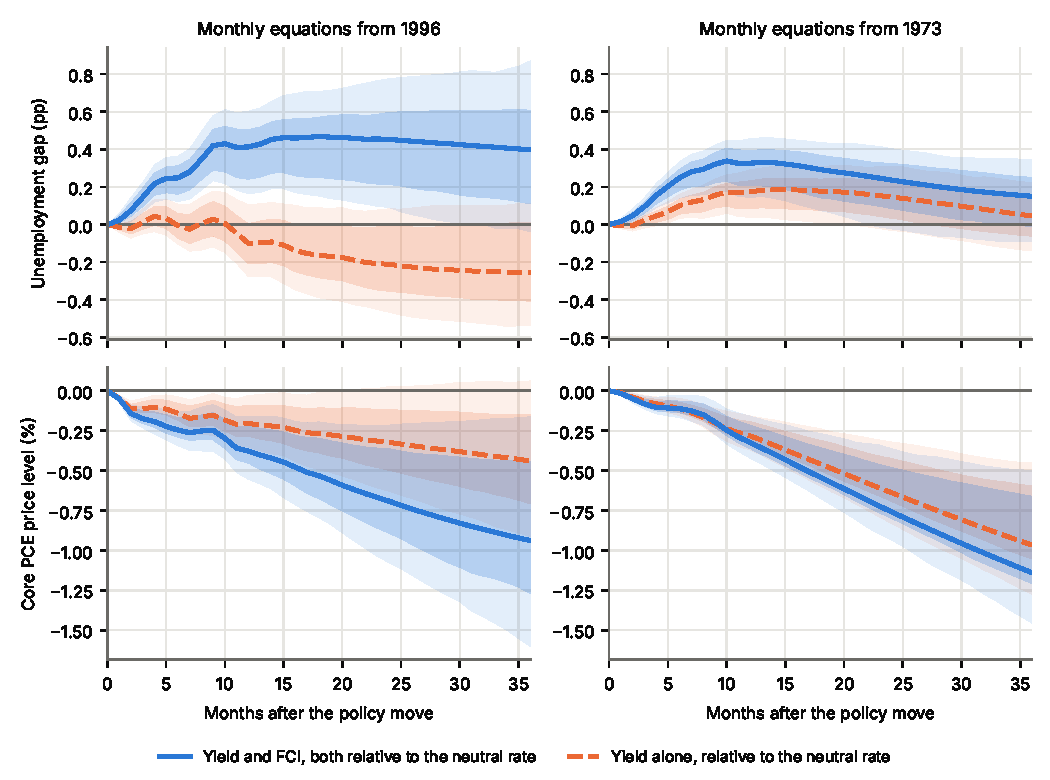
\includegraphics[width=\textwidth]{../baseline/report/fig_intro.pdf}
\caption{Responses to a Policy Move That Raises the Two-Year Yield 1 Percentage Point}
\label{fig:intro}
\begin{flushleft}\footnotesize\textit{Notes:} The move occurs in the window around the announcement. Blue: the surprise carried through the two-year yield and the financial conditions index, both relative to the neutral rate. Orange dashed: carried through the two-year yield alone, relative to the neutral rate. Left: monthly equations estimated from 1996; right: from 1973. Same surprise (the 252 announcements of 1996--2026), normalization, 12 monthly lags and bootstrap draws within each sample; March--December 2020 dropped. Shaded bands: 68 and 90 percent intervals.\end{flushleft}
\end{figure}

Four main conclusions emerge.
\begin{enumerate}\setlength\itemsep{0pt}
\item \textbf{Adding financial conditions reverses the estimated unemployment response.} In the data since 1996, where the wrong-signed response appears, adding financial conditions raises the two-year unemployment response by \bl{dc:nom:AC:u:24}, \bl{dc:real:AC:u:24} and \bl{dc:rstar:AC:u:24} percentage point in the nominal, real and neutral-rate versions, holding the surprise, sample and lag length fixed. With the FCI in the model, a tightening raises unemployment and lowers prices after a year under every variation of the sample, the neutral rate, the trend, credit conditions, the surprise and the lag length, from either starting date, and most of the estimates lie close to the baseline.
\item \textbf{Measuring rates against the neutral rate matters for prices.} The shift in unemployment is the same whether rates are nominal, real or relative to $\rs$. Measuring both the yield and the index relative to $\rs$ removes the common downward trend in rates and inflation and gives the largest fall in prices, about 0.7 percent after two years from either starting date.
\item \textbf{Lowering inflation costs less unemployment than recent estimates imply.} The sacrifice ratio of about one percentage-point year per 1 percent of the price level is a small fraction of the value of about 7 implied by high-frequency estimates for 1990--2008 \citep{barnichon2021}, and close to estimates for the decades before 1990.
\item \textbf{Policy shocks are a modest source of fluctuations.} Measured surprises explain almost none of the variation in unemployment and inflation. Policy-direction movements in rates and financial conditions explain about a tenth of it, and they mark the easing of 1979--80, the tightening of 1982--84 and the easing of 2020--21, which added about \bl{dc:hist:pi2122} percentage point to core inflation in 2021--22.
\end{enumerate}

The approach has three features. First, I measure the effect of each surprise in a short window around the announcement, when unemployment and inflation cannot move, and carry it forward in a daily and a monthly model estimated on ordinary data. As in \citet{jacobson2026}, the model takes into account when each announcement falls within its month. Second, financial conditions enter as a whole, as the transmission mechanism of standard models implies \citep{boivin2010}. The FCI combines the 10-year yield, equity valuation and the real dollar, weighted by their responses to policy news. Third, I measure the yield and the index relative to $\rs$, the real rate that neither speeds up nor slows down the economy. Interest rates trended down with $\rs$ from the 1990s to the 2010s \citep{laubach2003,holston2017,holston2023,hamilton2016,bauer2020,kiley2020} while activity trended up, and a model that links the level of rates to activity would partly pick up these opposite trends.

The results give the index of my companion paper \citep{fcinote} a use beyond describing conditions. Measured in units of a policy move and relative to $\rs$, financial conditions are the variable that standard estimates of transmission leave out.

Section~\ref{sec:tests} tests the approach against the alternatives. A tightening raises unemployment and lowers prices when the three components of the index enter separately, and under each of the four calibrations of the weights in the companion paper, which value the dollar relative to equities very differently.\footnote{From 1996 the price decline is smaller when the dollar is not tied to the long yield in the inflation equation; from 1973 it is about the same (Section~\ref{sec:components}).} With credit spreads added, in the monthly or the daily block, unemployment still rises and prices still fall. Tracking when in the month each announcement falls, the correction of \citet{jacobson2026}, adds most to the response once financial conditions are measured; without them unemployment still falls. Section~\ref{sec:rob} varies the sample, the measure of $\rs$, the trend, the surprise and the lag length.

\subsection{Connection to the Literature}
\textbf{Surprises and their effects.} Interest-rate surprises around FOMC announcements were meant to settle the measurement problem. The decision precedes the announcement, so market moves in a narrow window around it cannot have caused it \citep{kuttner2001,gurkaynak2005}. Such surprises measure the effects of policy on asset prices well \citep{bernanke2005,hanson2015,nakamura2018,swanson2021}, but for unemployment and inflation the old puzzles often return. Four explanations have been offered, each with a fix. Announcements reveal the Fed's view of the economy, and separating that information gives larger price effects \citep{romer2000,nakamura2018,jarocinski2020,miranda2021}. Part of each surprise is predictable, and removing it sharpens the estimates \citep{bauer2023,bauer2023aer}. Markets react in minutes while unemployment and inflation are monthly averages, and measuring inflation daily removes most of the wrong sign \citep{jacobson2026}. And credit costs, stock prices and the dollar carry part of the effect \citep{gertler2015,caldara2019,kroencke2021,bauer2023jep,boehm2024,bauer2026,boehm2026}. The conventional specifications that produce these puzzles trace the surprise through a single interest rate.

\textbf{What is new.} My paper is closest in spirit to \citet{jacobson2026}. Like them, I hold the surprise and the method fixed and change one measurement. They show that averaging daily data into months biases the estimated effects of policy, and they remove most of the price puzzle by measuring inflation with a daily price index. I change how the channel from policy to the economy is measured, and my main result is for activity. The two corrections are complementary. My model tracks when in the month each announcement falls, as they recommend, and that timing raises the unemployment response once financial conditions are in the model (Section~\ref{sec:timingtest}). Omitted financial channels and temporal aggregation are two sources of the puzzles, and correcting both gives the largest responses. \citet{bauer2023} and \citet{jarocinski2020} improve the surprise itself. In my design a surprise enters only through its immediate effect on the two-year yield and the FCI and through its timing, so their fixes and mine can be combined, and Section~\ref{sec:rob} does so.

\textbf{Financial channels and risk appetite.} \citet{gertler2015} show that policy surprises that move short rates modestly produce large movements in credit costs, through term premia and credit spreads. \citet{caldara2019} find that the response of activity to policy is weak and imprecise without the excess bond premium and conventional with it. \citet{bauer2026} find that monetary transmission appears to operate primarily through risk appetite and risk asset prices. My index carries the same channel through the prices that reveal it within the announcement window. The 10-year yield carries the term premium, and equity valuation carries the risk premium on the claims of firms that borrow. Credit spreads have no intraday series, so their response to policy news cannot be measured in the window, and a parsimonious index weighted by its response to policy keeps out movements unrelated to policy. Section~\ref{sec:credit} adds the excess bond premium and a daily credit spread, and a tightening still raises unemployment and lowers prices. Studies of the ``non-yield'' shock treat policy-driven moves in stock prices and the dollar as a second shock \citep{bauer2026,boehm2024}. \citet{boehm2026} select the combination of two yield-curve surprises and the non-yield shock that best accounts for macroeconomic fluctuations; they choose the direction of the shock for its macroeconomic content. I fix the conventional direction, news about the path of interest rates, and ask which financial variables are needed to trace it. My estimates are therefore conditional on that direction of news; they do not apportion business-cycle fluctuations among the shocks that announcements contain.

\FloatBarrier
% ============================================================
\section{Financial Conditions and the Empirical Approach}\label{sec:data}
This section explains why financial conditions should matter for the effects of policy, builds the index that measures them, shows what announcement windows reveal about it, and sets out the identifying assumptions and the model.

\subsection{Why Financial Conditions Matter for Monetary Policy}\label{sec:background}
The workhorse evidence on policy comes from VARs with a few macroeconomic variables and one interest rate \citep{bernanke1992,christiano1999}. Some studies add a credit spread \citep{gertler2015,caldara2019}, and factor models bring in many more series \citep{bernanke2005favar}. Long yields, equity valuations and the dollar are usually absent. Consider a rise in the two-year yield on an ordinary day. It comes with a modest tightening of broader financial conditions. Now consider the same rise on the day of an announcement. It comes with a much larger tightening, because a surprise about the path of policy moves long yields, stock prices and the dollar together. A model that observes only the yield cannot tell the two episodes apart. Leaving out the channel also misspecifies the model: if unemployment responds to financial conditions and not directly to the policy rate, the rate stands in for financial conditions, and the error contains past financial shocks that a VAR with few lags cannot capture (Appendix~\ref{app:toy}; \citealp{fernandez2007}). This differs from the omitted information about the economy that \citet{sims1992} proposed to explain the price puzzle; here the omitted variables are the channel itself.

Which financial prices move matters because they reach spending through different channels. Few households and businesses borrow at the policy rate. A household financing a home faces a mortgage rate tied to long yields; a firm valuing an investment faces a cost of capital set by long yields and equity prices; an exporter faces the dollar. Arbitrage links these rates to current and expected short rates. Higher rates raise the cost of capital and lower the value of existing capital \citep{jorgenson1963,hall1967,tobin1969}. Lower stock prices lower wealth and consumption \citep{ando1963,friedman1957}. A stronger dollar shifts spending toward imports \citep{fleming1962,mundell1963}. Modern models of the business cycle contain the same links \citep{christiano2005,smets2007,gali2005,kaplan2018,auclert2019}, and the effects come with a lag \citep{friedman1961}. The FOMC describes its policy in the same terms, as working through broad financial conditions.

Broad financial conditions indexes summarize this transmission \citep{hatzius2010,brave2011,ajello2023}, and credit spreads and asset prices help predict activity \citep{gilchrist2012,stock2003}. Such correlations need not be causal, because financial conditions also respond to the economy. The literature on high-frequency surprises has the opposite strength and weakness: it identifies policy shocks cleanly but carries them through few variables. I combine the two. The weights of my index come from how its components respond to policy news, and the surprise is carried forward through the estimated relationship between that index and the economy.

\textbf{Why relative to $r^*$.} What matters in these models is the real rate relative to the neutral rate, not the nominal rate. The same holds for the other parts of financial conditions: a given yield or stock valuation is tighter when $\rs$ is low. The distinction matters most for inflation, which responds to the slack that builds up over time and so to how long conditions stay tight relative to $\rs$. When real rates fall alongside the neutral rate, the decline in real rates alone makes the easing of financial conditions look larger than it was.

\subsection{The Financial Conditions Index}\label{sec:measure}
The FCI is the market index of my companion paper, \citet{fcinote}, which derives its weights and compares it with other indexes. I apply its method to the announcements of this paper. Indexes of this kind are weighted sums of financial variables, and they differ mainly in where the weights come from \citep{hatzius2010}. The best known in markets is the Goldman Sachs index \citep{dudley2000,hatzius2018}, whose published weights fall on the federal funds rate, the 10-year yield, a corporate spread, equity valuation and the dollar. FCI-G takes its weights from large macroeconomic models \citep{ajello2023}. Mine come from event-study regressions, long used to measure how asset prices respond to policy \citep{kuttner2001,bernanke2005,hanson2015,nakamura2018}.

\textbf{Why announcement windows.} The approach relies on one fact. In a narrow window around an FOMC announcement, the yield, stock prices and the dollar are all observed at high frequency, and policy news is the main systematic force moving them. The windows therefore reveal how the three respond to policy, and how large their joint movement is, without waiting for the economy to react. Unemployment and inflation cannot move in the window.

\textbf{Policy news.} Let $\Delta X_a$ be the $5\times 1$ vector of changes in the current- and next-meeting federal funds futures and the second to fourth eurodollar futures in the window around announcement $a$. Following \citet{nakamura2018}, let $p_a$ be the first principal component of these changes, signed so that it moves with the fourth eurodollar future. Policy news is $p_a$ rescaled so that one unit moves the two-year yield $y^{2}$ by 1 percentage point, in a regression with a constant:
\begin{equation}
s_a = \gamma\, p_a, \qquad \gamma = \frac{\sum_a (p_a-\bar p)(\Delta y^{2}_a-\overline{\Delta y^{2}})}{\sum_a (p_a-\bar p)^{2}}. \label{eq:ns}
\end{equation}

\textbf{Weights.} Let $\Delta A_a$ be the vector of changes in the 10-year yield, the S\&P 500 and the dollar index (DXY) in the window. Following the companion paper, I treat these changes as
\begin{equation}
\Delta A_a = \psi\, s_a + \eta_a, \label{eq:window}
\end{equation}
where $\psi$ holds the policy responses and $\eta_a$ is other news, with covariance matrix $\Sigma$. I estimate $\psi$ by regressing each element of $\Delta A_a$ on $s_a$ and a constant, and $\Sigma$ from the residuals, over the 252 announcements from January 1996 to July 2026 that I use throughout.\footnote{The companion paper also uses the announcement of September 2026 and scales $s_a$ without a constant. Its weights differ from mine by about 1 percent.} The weights are those that recover the policy component most precisely (one-factor generalized least squares):
\begin{equation}
w = \frac{\Sigma^{-1}\psi}{\psi'\Sigma^{-1}\psi}. \label{eq:weights}
\end{equation}
An asset gets more weight when it responds strongly to policy news and moves little for other reasons in the window, so the index is the combination of the three that tracks policy news most closely. Because $w'\psi=1$ and $s_a$ is scaled to the two-year yield, a policy move that raises the two-year yield 1 percentage point raises the index by 1 unit. The weights are 0.62 on the 10-year yield, $-0.052$ per percent on stock valuations and 0.066 per percent on the dollar, and each of the three accounts for about a third of the index's response to policy (Table~\ref{tab:weights}). Consider a hawkish surprise that raises the two-year yield 1 percentage point. On average it raises the 10-year yield about \bl{rv:psi:y10} percentage point, lowers stock valuations about \bl{rv:psi:equities} percent and raises the dollar about \bl{rv:psi:dollar} percent. Higher long rates raise the cost of borrowing for homes and investment, lower stock prices cut household wealth and raise the cost of equity, and a stronger dollar makes exports less competitive. The index adds these three tightenings into one number in units of the two-year yield. These shares describe how the three asset prices move on announcement days. Using the same weights in the monthly equations adds an assumption about how those prices affect the economy, which Section~\ref{sec:components} tests.

\begin{table}[tp]\centering\small
\caption{Market-Index Weights from Policy News}\label{tab:weights}
\resizebox{\ifdim\width>\textwidth\textwidth\else\width\fi}{!}{%
\begin{tabular}{lrrr}\toprule Component & Response to policy news & Weight & Share of a policy move\\ \midrule
10-year Treasury yield (pp) & $+$0.53 (0.06) & $+$0.616 & 0.33\\
Equity valuation, 100 ln CAPE (\%) & $-$7.71 (0.95) & $-$0.052 & 0.40\\
Real broad dollar, 100 ln (\%) & $+$4.18 (0.54) & $+$0.066 & 0.27\\
\bottomrule\end{tabular}}
\begin{flushleft}\footnotesize\textit{Notes:} Response of each 30-minute announcement-window change to the policy-news factor (scaled so the 2-year yield moves 1 pp), with robust standard errors; weights from the one-factor GLS of Kiley (2026); share = weight $\times$ response (the three shares sum to 1).\end{flushleft}
\end{table}


In month $t$, the index in version $v$ is
\begin{equation}
F_t^{v} = w_B\, B_t^{v} + w_Q\, Q_t^{v} + w_D\, D_t, \label{eq:fci}
\end{equation}
measured as a deviation from its sample mean. Here $B_t$ is the 10-year yield, $Q_t$ a measure of stock valuation and $D_t$ is 100 times the log of the real broad dollar in every version. The index comes in three versions, which differ in how the yield and stock prices are measured. I introduce them in turn, because each answers a problem with the one before.

\textbf{The nominal version.} The nominal version uses the nominal 10-year yield $y^{10}_t$ and measures stock valuation by the log of the cyclically adjusted price-earnings ratio (CAPE):
\begin{align}
\text{Nominal:}\quad & B_t = y^{10}_t, & Q_t &= 100\ln \text{CAPE}_t. \label{eq:nom}
\end{align}
It is the natural point of comparison with indexes built from nominal variables, and it has one problem: a trend. Nominal yields carry the inflation of the period. The 10-year yield was very high in the early 1980s, when expected inflation was high, and fell for decades after. Stock valuations moved the other way: CAPE was low in the early 1980s, when the earnings yield was high, and rose over the following decades. With a positive weight on the yield and a negative weight on valuation, both movements read as a steady loosening of conditions, and a trend alone explains \bl{tr:n:r2} percent of the variance of the nominal version. That trend is not a feature of financial conditions that policy affects. The part that comes from inflation is a feature of measuring them in nominal terms, and it motivates the real version; the part that comes from valuations motivates the version relative to $\rs$.

\textbf{The real version.} The real version subtracts 10-year expected inflation $\pi^{10}_t$ from the yield and leaves stock valuation as it is, because CAPE is already a real measure:
\begin{align}
\text{Real:}\quad & B_t = y^{10}_t - \pi^{10}_t, & Q_t &= 100\ln \text{CAPE}_t. \label{eq:real}
\end{align}
The real version removes the inflation in the yield, and with it part of the drift.

\textbf{The version relative to $r^*$.} The real index still trends: it falls over four decades (a trend explains \bl{tr:r:r2} percent of its variance), because real interest rates fell with the neutral rate and stock valuations rose. A real index reads a real rate of 1 percent in the 2010s as loose, but it was not loose if the neutral rate was lower still. Measuring the yield and stock valuation relative to $\rs$ removes that source of trend. The yield enters less expected inflation and less $\rs$. Stocks enter through the earnings yield, the inverse of CAPE, which I compare with $\rs$: stocks are expensive, and conditions loose, when the earnings yield is low relative to the neutral rate. That comparison enters with its sign reversed and is rescaled to the units of log CAPE, so the stock weight keeps its meaning:
\begin{align}
\text{$\rs$-gap (baseline):}\quad & B_t = y^{10}_t - \pi^{10}_t - \rs_t, & Q_t &= -\frac{100}{\overline{E/P}}\left[(E/P)_t - \rs_t\right]. \label{eq:rstar}
\end{align}
The term $100/\overline{E/P}$, with $\overline{E/P}$ the sample average, converts the earnings-yield gap to the units of log CAPE: since $d\ln\text{CAPE}=-d(E/P)/(E/P)$, a change in the earnings yield of $x$ points near the mean equals a change of $100x/\overline{E/P}$ in $100\ln\text{CAPE}$ with the opposite sign.

\textbf{A neutral level of the index.} \citet{caballero2026} define FCI$^*$, the neutral level of a financial conditions index consistent with output at potential, and show that gaps to it give useful guidance on the stance of policy, especially when financial conditions diverge from the policy rate. In their estimates on the FCI-G index, $\rs$ co-moves with the equity premium and FCI$^*$ does not. The version of my index relative to $\rs$ is a reduced-form counterpart of an index gap. Write $\tilde F_t$ for the index built from the real 10-year yield and the earnings-yield measure of valuation in equation~\eqref{eq:rstar} without $\rs$. Because $\rs$ enters the yield with weight $w_B$ and the earnings yield with weight $-w_Q\,100/\overline{E/P}$,
\begin{equation}
F^{\rs}_t = \tilde F_t - \kappa\, \rs_t, \qquad \kappa = w_B - w_Q\,\frac{100}{\overline{E/P}} = \bl{rv:kap}. \label{eq:fcistar}
\end{equation}
The index relative to $\rs$ is thus the gap between an index that ignores the neutral rate and a neutral level $\kappa\,\rs_t$, up to a constant. When $\rs$ falls 1 percentage point, the level of financial conditions that is neither tight nor loose falls \bl{rv:kap} units. This neutral level moves with the macroeconomic forces behind $\rs$ and not with asset prices, which is the property \citet{caballero2026} emphasize. It differs from their FCI$^*$ in that it is tied to an estimate of $\rs$ rather than estimated from the relationship between the index and the output gap.

\textbf{The two-year yield.} The two-year yield is adjusted in the same three versions. With $y^{2}_t$ the nominal yield and $\pi^{2}_t$ two-year expected inflation \citep[from the Cleveland Fed;][]{haubrich2012},
\begin{equation}
R_t^{\text{nominal}} = y^{2}_t, \qquad R_t^{\text{real}} = y^{2}_t - \pi^{2}_t, \qquad R_t^{\rs\text{-gap}} = y^{2}_t - \pi^{2}_t - \rs_t. \label{eq:twoyear}
\end{equation}
For $\rs$ I use the New York Fed's one-sided Laubach--Williams estimate \citep{holston2023}. It is a filtered estimate that uses data only up to each quarter, from the August 2026 vintage with parameters estimated on the full sample, so it is not a real-time series. Expected inflation and $\rs$ are monthly or quarterly and move slowly. The daily series add their interpolated monthly values to daily market prices, so day-to-day moves come from markets (Appendix~\ref{app:details}).

Figure~\ref{fig:fcis} plots the three versions on a common scale. Each step removes some of the downward drift: a trend explains \bl{tr:n:r2}, \bl{tr:r:r2} and \bl{tr:s:r2} percent of the variance of the nominal, real and $\rs$-relative versions. The versions do not differ at high frequencies; the correlation of 12-month changes is \bl{fci:c12:nr} between the nominal and real versions and \bl{fci:c12:rr} between the real version and the version relative to $\rs$. The differences are slow. The real version is below the nominal one by about 2 units around 1980, when expected inflation was highest, and the two are close after 1990. The version relative to $\rs$ is below the real version until the mid-2000s and above it by 1 to 2 units after 2010, as $\rs$ fell. Relative to their own historical means, the version relative to $\rs$ reads financial conditions after 2010 as one to two two-year-yield equivalents tighter than the real version. This is a difference in the level of the stance, which matters for prices because inflation depends on how long conditions stay tight. It is nearly invisible in changes, which is consistent with adding the FCI shifting the unemployment response by about the same amount in all three versions (Section~\ref{sec:baseline}).

\textbf{Comparison with the Goldman Sachs index.} A widely followed index offers a check on whether the approach captures what market participants mean by financial conditions. The companion paper rebuilds the Goldman Sachs index from public data with its published weights and shows that the rebuild mimics the published series closely \citep{fcinote}. The two indexes agree on changes: the correlation of 12-month changes is \bl{gs:n:l:chg} for the nominal versions and \bl{gs:r:l:chg} for the real versions from 1974. In levels the nominal versions agree since 1996 (\bl{gs:n:p:lev}) but less in 1974--95 (\bl{gs:n:e:lev}), when the two weight the inflation trend differently; the real versions agree closely throughout (\bl{gs:r:l:lev}). The close agreement in levels partly reflects shared inputs and a shared trend, so it shows that the measures agree, not that either is the right one for transmission. The agreement in changes, from weights derived in very different ways, is the more informative fact (Appendix Figure~\ref{fig:gs}).

\begin{figure}[tp]
\centering
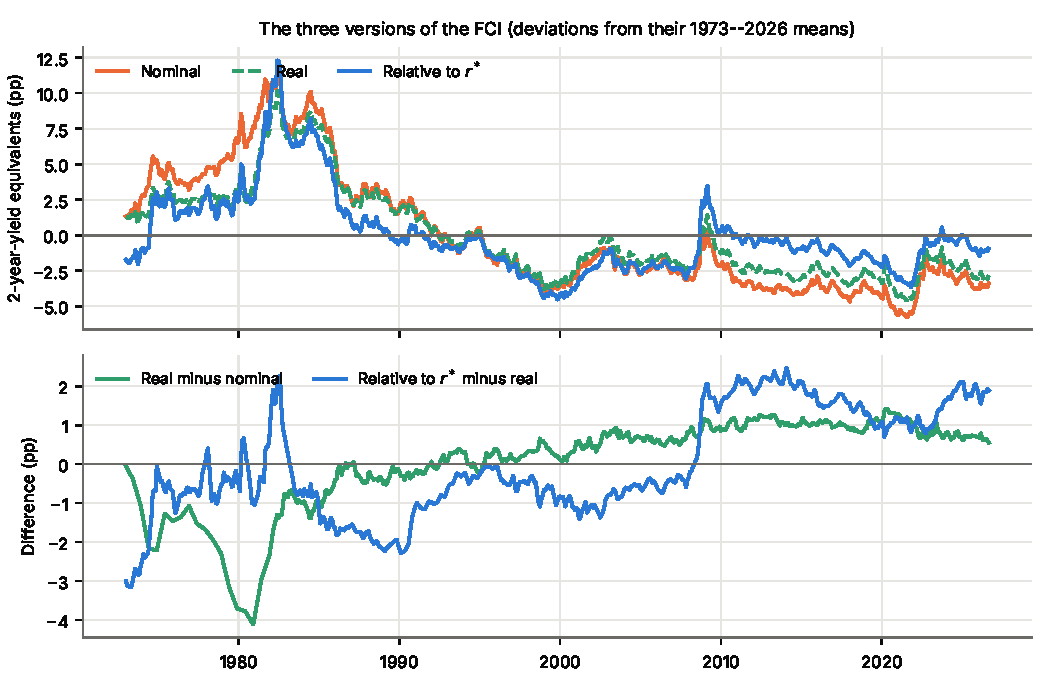
\includegraphics[width=0.9\textwidth]{../baseline/report/fig_fcis.pdf}
\caption{The Three Versions of the FCI}
\label{fig:fcis}
\begin{flushleft}\footnotesize\textit{Notes:} Monthly, in two-year-yield equivalents (a policy move that raises the two-year yield 1 percentage point raises each by one unit in the window). Each series is shown as a deviation from its mean over January 1973 to September 2026. Lower panel: real minus nominal, and relative to $\rs$ minus real.\end{flushleft}
\end{figure}

\subsection{One Rise in the Two-Year Yield, Two Days}\label{sec:resolve0}
Two facts from the windows drive the results. The first, and the central fact of the paper, is the size of the joint movement (Figure~\ref{fig:ordinary}).

\begin{center}
\fbox{\parbox{0.92\textwidth}{\textbf{An ordinary day and an announcement day.} On an ordinary day, the two-year yield rises 1 percentage point and financial conditions tighten by \bl{dc:rstar:ord} unit. On an announcement day, a policy surprise raises the two-year yield by the same 1 percentage point, and financial conditions tighten by \bl{dc:rstar:bF} unit, \bl{rv:ord:ratio} times as much, because long yields rise, stock prices fall and the dollar strengthens together. A model that sees only the two-year yield cannot tell the two days apart. It treats the policy surprise as an ordinary rise in rates and misses most of its financial consequences.}}
\end{center}

\begin{figure}[tp]
\centering
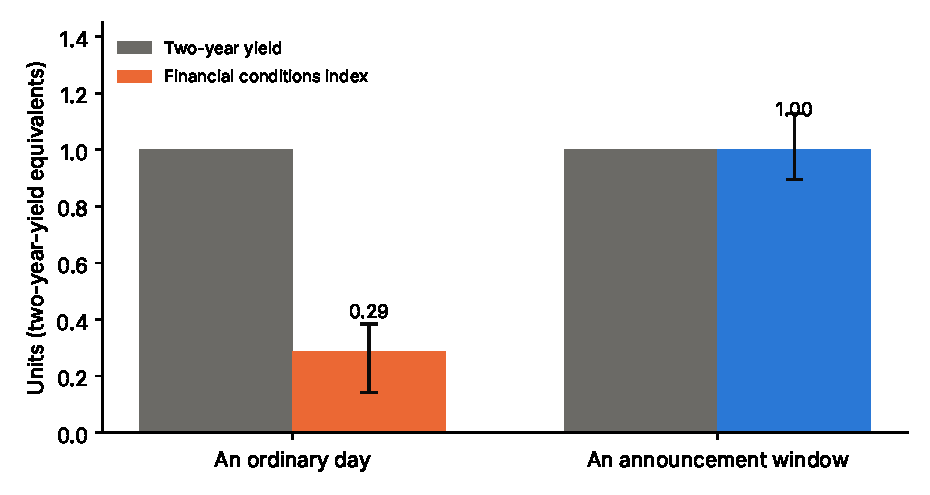
\includegraphics[width=0.72\textwidth]{../baseline/report/fig_ordinary.pdf}
\caption{The Same Rise in the Two-Year Yield on an Ordinary Day and an Announcement Day}
\label{fig:ordinary}
\begin{flushleft}\footnotesize\textit{Notes:} Change in the FCI relative to $\rs$ that accompanies a 1 percentage point rise in the two-year yield, in two-year-yield units. Ordinary day: the covariance of the daily-block innovations of the FCI and the yield divided by the variance of the yield innovation, on days without an announcement. Announcement window: the FCI's response to policy news divided by the yield's, over 252 announcements. Ranges: 90 percent bootstrap intervals ([\bl{dc:rstar:ord:lo}, \bl{dc:rstar:ord:hi}] and [\bl{rv:win:lo}, \bl{rv:win:hi}]).\end{flushleft}
\end{figure}

Why is the ordinary-day loading informative? The window loading is one by construction, because the weights are scaled to policy news. Nothing in that scaling fixes how the index moves with the yield on other days. On ordinary days the yield moves for many reasons, such as news about growth, inflation or risk appetite, and these move long yields, stocks and the dollar in offsetting ways; the loading measured on those days is an empirical fact about the data (Appendix~\ref{app:details}). On ordinary days the estimated loading is \bl{dc:rstar:ord}, with a 90 percent interval of \bl{dc:rstar:ord:lo} to \bl{dc:rstar:ord:hi}. A model with the yield alone learns how the economy responds to the yield from data in which a rise in the yield comes with little financial tightening, so it treats a policy surprise as an ordinary rise in rates. My design puts financial conditions in the system and measures the immediate effect of the surprise on both the yield and the FCI directly in the window.

The second fact is how much of the window movement the surprise explains. The interest-rate surprise explains \bl{r2:y2} percent of the window variation in the two-year yield and \bl{r2:fci} percent of the variation in the FCI, but only \bl{r2:y10} percent for the 10-year yield, \bl{r2:sp} percent for the S\&P 500 and \bl{r2:usd} percent for the dollar. Announcements move stock prices and the dollar by more than interest-rate surprises explain \citep{boehm2024,bauer2026}. The unexplained part is either news unrelated to policy, in which case my estimates capture the effects of policy, or policy news that does not move interest rates, in which case they capture one dimension of policy news and the effects of all of it could be larger. Both readings agree on the channel: policy news reaches the economy through broad financial conditions.

\subsection{Timing Assumptions and Identification}\label{sec:timing}
The shock is the Nakamura--Steinsson policy-news surprise, $s_a$ in equation~\eqref{eq:ns}, from the San Francisco Fed's U.S.\ Monetary Policy Event-Study Database \citep{acosta2025}. I use the 252 FOMC announcements from January 1996 to July 2026 with all the window measures available (Appendix~\ref{app:details}). The window runs from 10 minutes before the statement to 60 minutes after the press conference starts, or 30 minutes around the statement when there is no press conference. Identification comes from timing, at three frequencies, summarized in Table~\ref{tab:timing}.

\begin{table}[tp]\centering\small
\caption{Timing Assumptions}\label{tab:timing}
\begin{tabular}{p{0.12\textwidth}p{0.29\textwidth}p{0.38\textwidth}p{0.09\textwidth}}\toprule
Frequency & What can move & Assumption & Equation \\\midrule
Window (minutes) & Two-year yield and FCI, by the amounts measured in the window & News about the path of interest rates is the main systematic force in the window, and the only one correlated with the surprise. Unemployment and inflation do not move. & \eqref{eq:impact} \\[3pt]
Daily & Two-year yield and FCI, each day after the announcement & They depend on their own recent history and on the unemployment and inflation of this month and last month. & \eqref{eq:daily} \\[3pt]
Monthly & Unemployment and inflation, from the month after the announcement & Within a month, unemployment and inflation are set first. They respond to financial variables only with a lag of at least one month. & \eqref{eq:monthly} \\\bottomrule
\end{tabular}
\end{table}

\textbf{The window.} The window move in the FCI is computed with the weights in equation~\eqref{eq:weights}:
\begin{equation}
\Delta F_a = w_B\, \Delta y^{10}_a + w_Q\, \Delta \text{SP}_a + w_D\, \Delta \text{DXY}_a. \label{eq:winfci}
\end{equation}
These are the measures available within the day, and the ones used to estimate the weights. Percent changes in the S\&P 500 equal percent changes in CAPE within a window, because earnings are fixed. I express all effects per percentage point on the two-year yield in the window. The effect on the FCI is the ratio of two regression slopes on the surprise, an instrumental-variables estimate with $s_a$ as the instrument:
\begin{equation}
b = \begin{pmatrix} 1 \\ b_F \end{pmatrix}, \qquad b_F = \frac{\sum_a (\Delta F_a - \overline{\Delta F})\,(s_a-\bar s)}{\sum_a (\Delta y^{2}_a - \overline{\Delta y^{2}})\,(s_a-\bar s)} = 1. \label{eq:impact}
\end{equation}
This is one because the scaling in equation~\eqref{eq:ns}, the weights and this ratio use the same announcements and regressions with a constant. Expected inflation and $\rs$ move slowly, so I take the window move to be the same in every version.

\textbf{The day.} On the announcement day, the two-year yield and the FCI shift by the vector $b$. I use the window move and not the change over the whole day, because the full-day change contains other news. On later days the two series move as equation~\eqref{eq:daily} implies. They affect each other only through the daily lags, so no ordering between them is needed within the day.

\textbf{The month.} Within each month, unemployment and inflation are set first, and markets then respond to them. In the month of the announcement, unemployment and inflation therefore have not moved. They respond from the next month on, through the monthly average of the daily financial series. That average depends on when in the month the announcement falls, since an announcement late in a month affects few days of that month's average. This is how the model takes the timing of announcements into account, as \citet{jacobson2026} recommend. The ordering is the familiar recursive one, in which slow-moving macroeconomic variables come before financial variables \citep{bernanke1992,christiano1999}. The daily equations include the current month's unemployment and inflation, even though those figures are published later. I treat the monthly values as a summary of conditions that markets observe as the month unfolds.

\textbf{The main assumption.} The design thus has three steps: identify policy news in the window, measure its immediate financial effect $b$, and propagate that effect through daily and monthly equations estimated on ordinary days and months. Only the first two steps use the announcements. The third carries the main assumption: once the shock is identified, the economy responds to a change in the financial variables in the same way whatever caused it. A shock identified by a Cholesky ordering or an external instrument is carried through the same estimated dynamics as every other shock, and I do the same. Suppose stock prices fall 5 percent in an announcement window because the surprise raises the rate at which future earnings are discounted. On another day they fall 5 percent because earnings forecasts are cut. The first fall raises the cost of capital and lowers wealth with no news about demand. The second may also signal weaker demand, which would lower activity whatever the policy rate does. The model carries both through one equation. If the discount-rate fall is more or less contractionary than the average fall, the estimated propagation is wrong for the policy surprise. This problem differs from central-bank information, which concerns what $s_a$ reveals in the first step. \citet{bauer2023aer} show that what looks like an information effect largely reflects the Fed and markets responding to the same economic news, so that the surprises can be treated as policy news once that response is accounted for. I therefore use the surprises as they are. Section~\ref{sec:surprise} confirms that the results hold with their cleaned surprise and with the sign restriction of \citet{jarocinski2020}.

Two further assumptions are specific to this paper. First, the surprise reaches unemployment and prices only through the yield and the FCI, and has no direct effect on them in the window. Other channels, such as credit spreads and expectations, are left out; Section~\ref{sec:credit} adds them. So are moves in stock prices and the dollar that are unrelated to $s_a$. The non-yield shock of \citet{boehm2024} is uncorrelated with policy-news surprises, so such moves do not bias $b_F$. Second, the monthly equations see the FCI as a single index. Its weights show how the three components respond to policy news, not how the economy responds to each. I assume the three affect unemployment and prices in proportion to those weights, and Section~\ref{sec:components} tests that.

\subsection{A Mixed-Frequency VAR}\label{sec:midas}
Financial markets process policy news in minutes, while unemployment and prices take months to respond. The model therefore runs on two clocks. A daily block tracks the immediate repricing of the two-year yield and the FCI and how long that repricing lasts. A monthly block measures how the accumulation of these daily conditions shifts unemployment and inflation, which in turn feed back into the markets of the following month. The announcement enters on the day it occurs, so the model knows whether a surprise came early in a month, when it moves most of that month's financial conditions, or late, when it moves few of them. The equations below make these two clocks precise.

\textbf{Structure.} The model has a daily block and a monthly block. Let $x_\tau=(R_\tau,F_\tau)'$ hold the two-year yield and the FCI on day $\tau$, in the same version. Let $m_t=(U_t,\pi_t)'$ hold the two monthly variables. The unemployment gap $U_t$ is the unemployment rate minus the CBO estimate of its natural rate. The CBO estimate does not respond to the surprise, so the response of the gap equals that of the unemployment rate. Inflation is $\pi_t=1200\,\Delta\ln P_t$, where $P_t$ is the price index for personal consumption expenditures excluding food and energy (core PCE).

The daily block is a VAR that uses averages of the past day, week, month and quarter as regressors \citep{corsi2009}:
\begin{equation}
x_\tau = \alpha + \sum_{k\in\{1,5,22,66\}} \Phi_k\, \bar x_{\tau-1}^{(k)} + \Gamma_0\, m_{t(\tau)} + \Gamma_1\, m_{t(\tau)-1} + \xi_\tau, \label{eq:daily}
\end{equation}
where $\bar x_{\tau-1}^{(k)}$ is the average of $x$ over the $k$ days through $\tau-1$, and $t(\tau)$ is the month of day $\tau$. Averages over about a day, a week, a month and a quarter capture persistence with few coefficients, which matters because how long the financial movement lasts determines how much of it reaches the monthly averages. When the FCI is left out, $x_\tau$ is the two-year yield alone.

The monthly block is
\begin{equation}
m_t = c + \sum_{l=1}^{L} A_l\, m_{t-l} + \sum_{l=1}^{L} G_l\, \bar x_{t-l} + \zeta_t, \qquad \bar x_{t}=\frac{1}{n_t}\sum_{\tau\in t} x_\tau, \label{eq:monthly}
\end{equation}
with $n_t$ the number of weekdays in month $t$. The model is a mixed-frequency VAR \citep{ghysels2016}. The equation contains no current-month term in $\bar x_t$, which is the timing assumption of Table~\ref{tab:timing}.

\textbf{The time trend.} The baseline monthly equations contain a constant and no time trend. Rates drifted down along with $\rs$ over 1996--2026, and the $\rs$ adjustment is meant to remove that drift from the financial variables, which is the work a trend would otherwise do. A trend could still matter for other reasons: inflation was low in the 2010s and rose after 2020, and the natural rate of unemployment may have shifted in ways the CBO estimate misses. Section~\ref{sec:rstarrob} replaces the $\rs$ adjustment with a spline trend.

\textbf{How the responses are computed.} The response to a policy surprise is traced day by day. On the announcement day the yield and the FCI jump by the window impact $b$ and the macro variables are at their no-surprise values. Each later day, the daily equation gives the two financial series from their own recent averages and from the macro variables of the month. At the end of each month the monthly average of the daily financial series enters the monthly equations, which give the next month's unemployment and inflation. Those feed back into the daily equations of the following month. The response is the difference from a path with no surprise. Because the model is linear, the response to a surprise of any size is a multiple of the response to a unit surprise. I average the responses over the positions of the announcements within their months, as in the data, because an announcement early in a month moves that month's average more than a late one. The response of the price level after $h$ months is $\sum_{j=0}^{h}\tilde\pi_j/12$.

\textbf{Relation to a monthly VAR.} If every announcement fell on the first day of its month and the daily block were replaced by a monthly equation, the model would be a standard monthly VAR with a recursive ordering. The daily block adds the position of each announcement in its month and the fast dynamics of the financial variables, which it estimates on many more observations. A proxy VAR instead estimates the effect of the surprise on every variable from monthly residuals. Two facts favor starting the system from the window. The surprise is a weak instrument for monthly residuals, so a proxy VAR has wide sets, and a direct projection of the outcomes on the surprise is imprecise and changes sign with its controls. Measuring the impact in the window, where the surprise explains most of the movement, and estimating the propagation on ordinary data uses the information each source has. Section~\ref{sec:monthlyvar} estimates both monthly benchmarks, and Appendix~\ref{app:relation} gives the algebra.

\textbf{Why the window, and not monthly innovations.} A monthly VAR recovers a policy shock from the month's innovations, and that requires the shock to be a combination of those innovations (invertibility). Starting the model from the window does not: the shock is observed directly, and the model only has to propagate it. The requirement fails in these data. The month's sum of the measured surprises explains \bl{dc:diag:rstar:yes:1996:r2} percent of the month's VAR innovations, and the shock recovered from those innovations has a correlation of \bl{dc:diag:rstar:yes:1996:corr} with the surprise. The same happens in samples simulated from the model itself, where the policy shock is the window surprise by construction (median $R^2$ of \bl{dc:sim:r2_z_u:med} percent; Appendix~\ref{app:relation}). The failure is a property of how a surprise concentrated on one day enters monthly data, not of these data.

\textbf{Estimation and inference.} I estimate each block by ordinary least squares. The daily block uses the weekdays from January 1996, the month of the first announcement with all window measures, to September 2026. The monthly equations have two samples, which give the two baselines: from January 1996 (\bl{nobs} months) and from January 1973 (\bl{b73:nobs} months). In the longer sample the months before 1990 use monthly series in place of the daily block (Appendix~\ref{app:details}); the daily block, the announcements and the window impacts are those of 1996--2026 in both. The lagged daily averages and the monthly lags may use earlier observations. Both blocks leave out March to December 2020, which is the same as a dummy for each of those months: the pandemic moved unemployment by more in those months than in any other episode, for reasons unrelated to financial conditions. The 2020 values still enter as lags, and Section~\ref{sec:rob} keeps them in. The baseline has $L=12$ monthly lags, fixed in advance. Fewer lags give the same signs and weaker evidence (Section~\ref{sec:surprise} and Appendix~\ref{app:lags}).

Intervals come from a block bootstrap with 500 draws \citep{kunsch1989,jentsch2019}. Each draw resamples the calendar months from 1996 in blocks of 12 and uses together the monthly residuals, the daily observations and the announcements of the months drawn. That keeps the dependence among them. In the sample from 1973 the residuals of the months before 1996 are drawn in blocks of 12 of their own. The monthly equations and the daily block are re-estimated on each draw; the FCI weights and $\rs$ are held fixed. A response is significant at the 5 or 10 percent level when its 95 or 90 percent interval excludes zero. I report 90 percent intervals, as recent studies in this area do \citep{bauer2023,caldara2019,miranda2021,ramey2016}, and 68 percent intervals, which \citet{jarocinski2020} report alongside them. Appendix~\ref{app:boot} compares a simpler bootstrap.

\textbf{Data.} All inputs are public series (Appendix~\ref{app:data}). Daily market data are the 2-year and 10-year Treasury yields, the S\&P 500 and the broad dollar index. Monthly data are the unemployment rate, the CBO estimate of its natural rate, core PCE inflation, expected inflation from the Cleveland Fed and the neutral-rate estimates. Policy news comes from the San Francisco Fed's event-study database. For the sample from 1973, the months before 1990 use monthly series in place of the daily block. All monthly financial variables are monthly averages of the daily series, in the model and in every benchmark.

\FloatBarrier
% ============================================================
\section{Results}\label{sec:results}
% Numbers in this section are macros from baseline/report/numbers.tex; the qualitative claims are asserted in baseline/07_report.py (check_claims), which fails if they stop being true.
Four results follow. Standard methods, applied to my data since 1996, give a tightening the wrong effect on unemployment. Adding the FCI reverses it, by about the same amount whichever yield is used, and over the longer sample from 1973 it enlarges responses that already have conventional signs. The responses with the FCI imply a moderate cost of lowering inflation. And policy-direction movements in rates and financial conditions account for a modest share of fluctuations in unemployment and inflation.

\subsection{Standard Methods after the Early 1980s}\label{sec:standard}
Standard identification schemes have not delivered conventional effects of monetary policy in samples that start after the early 1980s. \citet{ramey2016} estimates the specification of \citet{christiano1999} on 1983--2007 and finds that ``the results change dramatically and imply that increases in the federal funds rate lower the unemployment rate''; other schemes she examines give contractionary shocks that look expansionary, as \citet{barakchian2013} found for 1988--2007, or a pronounced price puzzle. The literature reads this either as a change in the economy, with policy responding more systematically and expectations better anchored \citep{boivin2006,boivin2010,primiceri2005}, or as a failure of identification once policy became forward-looking \citep{barakchian2013}. One finding points to measurement. \citet{caldara2019} find, for 1994--2007 with a proxy SVAR that uses high-frequency surprises, that the response of industrial production is weak and uncertain without a credit spread (about $-0.2$ percent, with a credible set that includes positive values) and about $-0.75$ percent when the excess bond premium is added.

I start from two standard methods, estimated on my own data so that they compare directly with the model below. Both use the monthly unemployment gap, core PCE inflation and the monthly average of the two-year Treasury yield, with 12 lags, no trend and March to December 2020 left out, on the two samples of the model, from 1996 and from 1973. The first is the recursive (Cholesky) VAR of \citet{christiano1999}, with the policy rate ordered last; its responses are to a 1 percentage point rise in the monthly yield. The second is a proxy VAR \citep{stock2018,mertens2013,gertler2015} that uses the Nakamura--Steinsson surprise, summed over the announcements of the month, as an instrument for the policy rate; its responses are to a surprise that raises the yield 1 percentage point in the announcement window, the unit of the model.\footnote{A window move of 1 percentage point raises the month's average yield by about \bl{mo:win} in the model, because the announcement falls on average in the middle of the month. The first-stage $F$ statistic of the proxy VAR is \bl{st:prox:F} from 1996 and \bl{st:prox73:F} from 1973, so I report exact Anderson--Rubin sets, which stay valid when the instrument is weak \citep{montiel2021,lunsford2015,lewis2026,bauer2026}.} Figure~\ref{fig:standard} shows the responses since 1996, and Table~\ref{tab:standard} reports both samples.

\begin{figure}[tp]
\centering
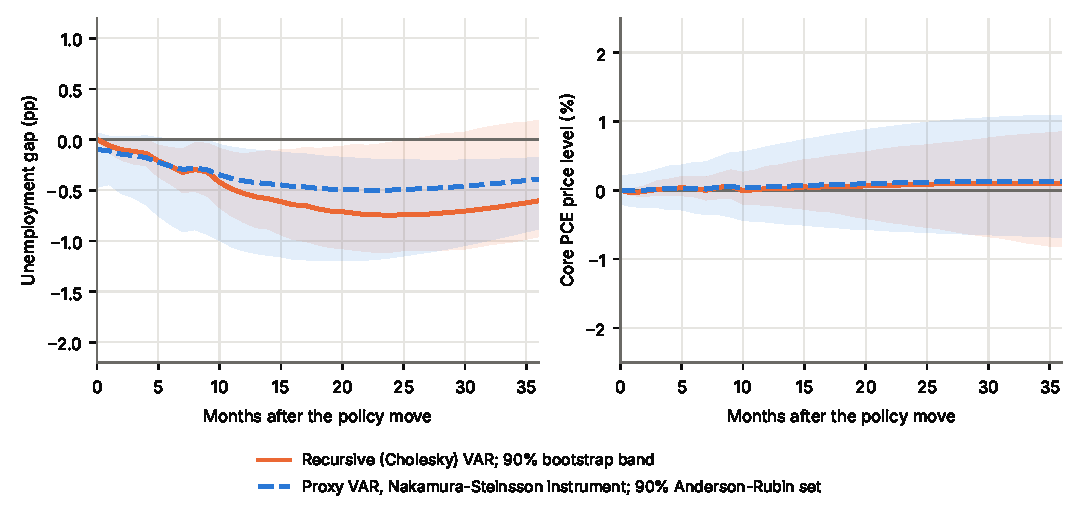
\includegraphics[width=\textwidth]{../baseline/report/fig_standard.pdf}
\caption{Standard Methods: Responses to a 1 Percentage Point Rise in the Two-Year Yield, 1996--2026}
\label{fig:standard}
\begin{flushleft}\footnotesize\textit{Notes:} Recursive (Cholesky) VAR and proxy VAR with the Nakamura--Steinsson instrument, in the monthly unemployment gap, core PCE inflation and the monthly average of the two-year yield; 12 lags; March--December 2020 dropped. Bands: 90 percent (bootstrap for the Cholesky VAR, Anderson--Rubin sets for the proxy VAR, truncated at $\pm4$).\end{flushleft}
\end{figure}

\begin{table}[tp]\centering\footnotesize\setlength{\tabcolsep}{2.4pt}
\caption{Standard Methods: Responses to a 1 Percentage Point Rise in the Policy Rate}\label{tab:standard}
\resizebox{\ifdim\width>\textwidth\textwidth\else\width\fi}{!}{%
\begin{tabular}{llrrrrrrr}\toprule
 & & & \multicolumn{3}{c}{Unemployment gap (pp)} & \multicolumn{3}{c}{Price level (\%)}\\ \cmidrule(lr){4-6}\cmidrule(lr){7-9}
Method & Sample & Obs & 12 m & 24 m & 36 m & 12 m & 24 m & 36 m\\ \midrule
Cholesky, 2-year yield & 1996--2026 & 369 & $-$0.95$^{*}$ & $-$0.66$^{*}$ & $-$0.36 & 0.13 & 0.07 & $-$0.10\\
 & & & {\scriptsize [$-$1.50, $-$0.40]} & {\scriptsize [$-$1.10, $-$0.12]} & {\scriptsize [$-$0.75, 0.21]} & {\scriptsize [$-$0.12, 0.36]} & {\scriptsize [$-$0.40, 0.52]} & {\scriptsize [$-$0.72, 0.56]}\\
Proxy VAR, 2-year yield & 1996--2026 & 369 & $-$0.91$^{*}$ & $-$0.61$^{*}$ & $-$0.32 & 0.03 & $-$0.08 & $-$0.26\\
 & & & {\scriptsize [$-$1.38, $-$0.42]} & {\scriptsize [$-$1.08, $-$0.05]} & {\scriptsize [$-$0.71, 0.17]} & {\scriptsize [$-$1.20, 0.97]} & {\scriptsize [$-$1.84, 1.26]} & {\scriptsize [$-$2.28, 1.26]}\\
\bottomrule\end{tabular}}
\begin{flushleft}\footnotesize\textit{Notes:} Monthly data, 12 lags, constant, no trend; unemployment gap, core PCE inflation and the end-of-month policy rate (the 2-year Treasury yield, or the effective federal funds rate where stated), policy rate ordered last in the Cholesky VARs; price level = cumulated inflation/12. Proxy VAR: Nakamura--Steinsson policy news summed within the month as instrument; first-stage $F$ = 4.5. Unit: +1 pp on the policy rate on impact. Brackets: 90\% intervals (residual bootstrap for the Cholesky VARs; exact Anderson--Rubin sets for the proxy VAR). $^{*}$ = excludes zero.\end{flushleft}
\end{table}


Since 1996 both reproduce the puzzle. Unemployment falls after a tightening, by \blabs{st:c2y96:u:12} percentage point after 12 months in the Cholesky VAR and \blabs{st:prox:u:12} in the proxy VAR, and it is still lower after 24 months. The price level does not respond. Starting in 1984 gives a smaller fall in unemployment, a funds-rate version on 1984--2007 gives the same sign, and adding commodity prices, the standard remedy for the price puzzle \citep{sims1992,ramey2016}, leaves the response negative (Appendix Tables~\ref{tab:standardall} and~\ref{tab:standardcom}). From 1973 the picture is different: the Cholesky VAR gives unemployment slightly higher and prices slightly lower after a tightening (\bl{st:c2y73:u:12} percentage point and \bl{st:c2y73:P:24} percent), and the proxy VAR, with an instrument that explains little of the monthly residuals over the long sample, is uninformative. The wrong signs are a feature of the sample since 1996 when the surprises are carried through the two-year yield alone.

\subsection{The FCI Model: Baseline Results}\label{sec:baseline}
Traced through the FCI, a tightening raises unemployment and lowers prices, whether the yield is measured in nominal terms, in real terms or relative to $\rs$. Table~\ref{tab:matched} gives the matched comparison for both samples: for each version, the responses after 24 months with the yield alone and with the yield and the FCI, on common bootstrap draws within each sample.

\begin{table}[tp]\centering\footnotesize\setlength{\tabcolsep}{3pt}
\caption{Responses without and with the FCI after Two Years}\label{tab:matched}
\resizebox{\ifdim\width>\textwidth\textwidth\else\width\fi}{!}{%
\begin{tabular}{lcccccc}\toprule
 & \multicolumn{3}{c}{Unemployment gap (pp)} & \multicolumn{3}{c}{Price level (\%)}\\ \cmidrule(lr){2-4}\cmidrule(lr){5-7}
Yield measure & Yield alone & Yield and FCI & Difference & Yield alone & Yield and FCI & Difference\\ \midrule
Nominal & $-$0.45$^{**}$ & 0.16 & 0.62$^{**}$ & 0.06 & $-$0.29 & $-$0.35$^{*}$\\
 & {\scriptsize [$-$0.69, $-$0.17]} & {\scriptsize [$-$0.08, 0.49]} & {\scriptsize [0.34, 0.90]} & {\scriptsize [$-$0.21, 0.40]} & {\scriptsize [$-$0.69, 0.10]} & {\scriptsize [$-$0.75, $-$0.05]}\\
\addlinespace
Real & $-$0.35$^{**}$ & 0.23$^{*}$ & 0.57$^{**}$ & $-$0.06 & $-$0.38$^{**}$ & $-$0.32$^{*}$\\
 & {\scriptsize [$-$0.57, $-$0.11]} & {\scriptsize [0.00, 0.50]} & {\scriptsize [0.33, 0.86]} & {\scriptsize [$-$0.28, 0.21]} & {\scriptsize [$-$0.75, $-$0.07]} & {\scriptsize [$-$0.66, $-$0.05]}\\
\addlinespace
Neutral rate ($r^*$-gap) & $-$0.21 & 0.45$^{**}$ & 0.66$^{**}$ & $-$0.32 & $-$0.69$^{**}$ & $-$0.37\\
 & {\scriptsize [$-$0.47, 0.08]} & {\scriptsize [0.09, 0.78]} & {\scriptsize [0.27, 1.00]} & {\scriptsize [$-$0.63, 0.03]} & {\scriptsize [$-$1.08, $-$0.21]} & {\scriptsize [$-$0.72, 0.03]}\\
\bottomrule\end{tabular}}
\begin{flushleft}\footnotesize\textit{Notes:} Responses 24 months after a policy move that raises the two-year yield 1 pp in the window, 1996--2026, 12 lags. Differences are computed on common bootstrap draws before rounding. Brackets: 90\% intervals; $^{**}$, $^{*}$: 5 and 10 percent levels. Responses at 12 and 36 months and at 3 and 6 lags are in Appendix Tables~\ref{tab:mainB} and~\ref{tab:lags}.\end{flushleft}
\end{table}


Start with the sample since 1996. With the nominal or real yield alone the model gives what the standard methods give: unemployment falls and the price level does not respond. Measured relative to $\rs$, the yield alone lowers the price level, by \blabs{rstar:no:P:24} percent after two years, but still does not raise unemployment. That the adjustment helps prices first is what the reasoning of Section~\ref{sec:background} leads one to expect: removing the common downward trend in rates and inflation removes a spurious link between low rates and low inflation, and inflation depends on how long conditions stay tight. Adding the FCI moves both responses by nearly the same amount in every version. It raises the unemployment response after 24 months by \bl{dc:nom:AC:u:24}, \bl{dc:real:AC:u:24} and \bl{dc:rstar:AC:u:24} percentage point in the nominal, real and neutral-rate versions, and it lowers the price response by \bl{dc:nom:AC:P:24:abs}, \bl{dc:real:AC:P:24:abs} and \bl{dc:rstar:AC:P:24:abs} percent. The matched shift is more stable than the level of the response, which depends on how the yield is measured: the neutral-rate version, which with the yield alone has the smallest fall in unemployment and the largest fall in prices, ends with the largest responses, \bl{rstar:yes:u:24} percentage point and \bl{rstar:yes:P:24} percent. The size also depends on how long the financial movement lasts: with an FCI path that decays as fast as the direct evidence on the days after announcements allows, the baseline unemployment response after 24 months is \bl{pe:rho:pt:u24} rather than \bl{pe:rho:base:u24} (Section~\ref{sec:resolve}).

The sample from 1973 starts from a different place. There the yield alone already gives a tightening conventional effects: in the neutral-rate version unemployment is \bl{b73:rstar:no:u:12} percentage point higher after a year and the price level \blabs{b73:rstar:no:P:24} percent lower after two. Adding the FCI raises the 12-month unemployment response by \bl{m73:nom:AC:u:12}, \bl{m73:real:AC:u:12} and \bl{m73:rstar:AC:u:12} percentage point in the three versions, again nearly the same amount, and deepens the 24-month price fall by \bl{m73:rstar:AC:P:24:abs} percent in the neutral-rate version. The two samples agree on prices: with the yield and the FCI relative to $\rs$, the price level falls \blabs{rstar:yes:P:24} percent after two years from 1996 and \blabs{b73:rstar:yes:P:24} percent from 1973. The unemployment response from 1973 is somewhat smaller after a year (\bl{b73:rstar:yes:u:12} against \bl{rstar:yes:u:12}) and fades sooner. Over five decades, financial conditions add to effects that the yield already carries; since 1996, they supply effects that the yield alone gets wrong.

Figure~\ref{fig:steps} shows the paths behind the table. The responses build over the first year and a half and then stabilize or continue, and in every version the FCI moves the unemployment path above the yield-alone path from the first months. Appendix Table~\ref{tab:mainB} gives 12, 24 and 36 months.

\begin{figure}[tp]
\centering
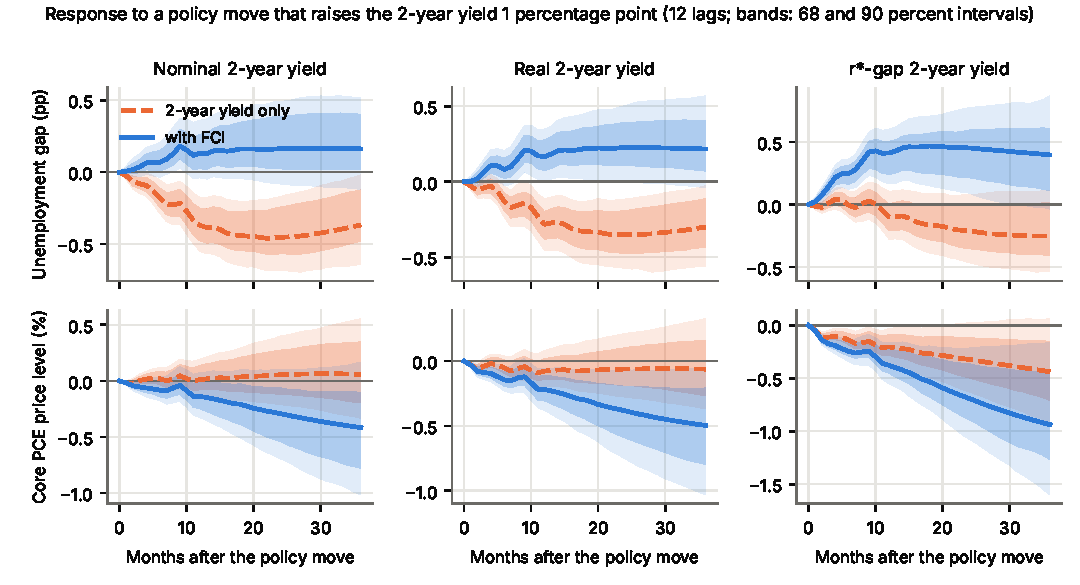
\includegraphics[width=\textwidth]{../baseline/report/fig_steps.pdf}
\caption{Responses to a Policy Move, without and with the FCI}
\label{fig:steps}
\begin{flushleft}\footnotesize\textit{Notes:} Policy move that raises the two-year yield 1 percentage point in the window; 12 lags. Orange dashed: the yield alone. Blue: the yield and the FCI of the same version. Bands: 68 and 90 percent intervals.\end{flushleft}
\end{figure}

\textbf{How large are these effects?} A surprise of 1 percentage point on the two-year yield is large: the standard deviation of the surprises is \bl{sd:ns:bp} basis points, and 90 percent of them are below \bl{sd:ns:p90} basis points. I report responses per percentage point because the model is linear and because that unit matches how policy is discussed; the Federal Reserve raised its policy rate by more than 5 percentage points in 2022--23. The responses describe how a policy move of a given size is transmitted, not the effect of any one announcement. They are larger than, and consistent with, the closest estimates in the literature. \citet{bauer2023} remove the predictable part of the surprise and carry it through a monthly VAR with the end-of-month two-year yield, which moves nearly one for one with a window surprise, so the unit matches mine closely. Rescaled to a 1 percentage point rise in the yield, their benchmark gives unemployment about 0.17 percentage point higher and the consumer price index about 0.5 percent lower after 24 months (their Figure~8). Both values lie inside the 90 percent intervals of the baseline (Table~\ref{tab:matched}). They obtain conventional signs by cleaning the surprise; I obtain them by tracing its financial effects, and Section~\ref{sec:surprise} shows that the two fixes combine.

\subsection{The Implied Inflation-Unemployment Tradeoff}\label{sec:tradeoff}
Once a tightening raises unemployment and lowers prices, the two responses together measure the cost of disinflation. The question is central to current policy. The inflation surge of 2021--22 has been attributed mostly to a tight labor market \citep{benigno2023,ball2022} or mostly to shocks to prices \citep{blanchard2023}, and the two readings imply very different costs of bringing inflation down. \citet{benigno2023} argue that appropriate policy can lower inflation without a significant recession; \citet{ball2022} find that returning inflation to target requires optimistic assumptions about expectations and the labor market. The answer depends on how much unemployment accompanies a given fall in prices. Recent work finds a small Phillips-curve slope \citep{hazell2022,delnegro2020,ball2019,fitzgerald2024}, which would make lowering inflation costly. The slope is hard to identify when policy offsets demand shocks \citep{mcleay2020}, and conventional methods understate it \citep{barnichon2020}. \citet{barnichon2021} measure the tradeoff directly, by the ratio of the price response to the cumulative unemployment response after a policy shock. I follow them and use their Phillips multiplier at horizon $H$:
\begin{equation}
\mathcal{P}_H = \frac{\tilde P_H}{\tilde U_H}, \qquad \tilde U_H=\frac{1}{12}\sum_{h=1}^{H}\tilde U_h, \label{eq:pm}
\end{equation}
where $\tilde P_H$ is the response of the core price level after $H$ months, in percent, and $\tilde U_H$ is the cumulative response of the unemployment gap, in percentage-point years. A larger price decline for the same cumulative unemployment response gives a larger multiplier in absolute value. The multiplier is not the slope of a Phillips curve alone, because import prices and expectations can also carry the price response. Its inverse, $-1/\mathcal{P}_H$, is a sacrifice ratio: the percentage-point years of unemployment that come with a 1 percent lower price level. The unit is the price level at a stated horizon, not a permanent fall in the inflation rate. When $\tilde U_H$ is close to zero the ratio is not well defined, so I form 90 percent sets for $\mathcal{P}_H$ in the spirit of \citet{anderson1949}: the set contains every value $\mathcal{P}$ for which the 90 percent bootstrap interval of $\tilde P_H-\mathcal{P}\,\tilde U_H$ contains zero.

\begin{table}[tp]\centering\footnotesize\setlength{\tabcolsep}{3pt}
\caption{Implied Trade-Off: The Phillips Multiplier}\label{tab:tradeoff}
\resizebox{\ifdim\width>\textwidth\textwidth\else\width\fi}{!}{%
\begin{tabular}{lcccc}\toprule
 & \multicolumn{2}{c}{24 months} & \multicolumn{2}{c}{36 months}\\ \cmidrule(lr){2-3}\cmidrule(lr){4-5}
Yield and FCI, measured as & Estimate & 90\% set & Estimate & 90\% set\\ \midrule
Nominal & $-$1.21 & undefined; 68\%: [$-$3.29, $-$0.30] & $-$1.03 & undefined; 68\%: [$-$2.96, $-$0.31]\\
Real & $-$1.16 & [$-$5.51, $-$0.25] & $-$0.90 & [$-$7.04, $-$0.07]\\
\textbf{Neutral rate, 1996 start (baseline)} & \textbf{$-$0.95} & \textbf{[$-$1.99, $-$0.32]} & \textbf{$-$0.81} & \textbf{[$-$2.12, $-$0.18]}\\
Neutral rate, 1973 start & $-$1.49 & [$-$2.92, $-$0.72] & $-$1.64 & [$-$5.39, $-$0.72]\\
\bottomrule\end{tabular}}
\begin{flushleft}\footnotesize\textit{Notes:} $\kappa_H$ is the core PCE price level at month $H$ (percent) per percentage-point year of cumulative unemployment-gap response \citep{barnichon2021}; its inverse in absolute value is the sacrifice ratio. Estimate: ratio of the point responses. 90\% set: Anderson--Rubin type, all values for which the 90\% bootstrap interval of $\tilde P_H-\kappa\tilde U_H$ contains zero. The ratio is undefined when the 90\% interval of the cumulative unemployment response includes zero, because the data then cannot rule out unemployment responses of zero or either sign; the 68\% set is then shown where it exists. 12 lags. All cases in Appendix Table~\ref{tab:tradefull}.\end{flushleft}
\end{table}


The point estimates of the tradeoff are close across versions and samples. With the yield and the FCI relative to $\rs$, $\mathcal{P}_{24}$ is \bl{tr:rstar:yes:24} in the sample since 1996 and \bl{tr73:rstar:yes:24} in the sample from 1973; with the real yield and FCI it is \bl{tr:real:yes:24} and \bl{tr73:real:yes:24} (Table~\ref{tab:tradeoff}). The sacrifice ratio after two years is therefore about one percentage-point year of unemployment per 1 percent lower price level: \bl{tr:sac:24} from 1996, with a set of \bl{tr:sac:24:lo} to \bl{tr:sac:24:hi}, and \bl{tr73:sac:24} from 1973, with a set of \bl{tr73:sac:24:lo} to \bl{tr73:sac:24:hi}. After three years it is \bl{tr:sac:36} and \bl{tr73:sac:36}.\footnote{In the sample from 1996 the price decline behind this ratio is smaller when the dollar is not tied to the long-term yield in the inflation equation (Section~\ref{sec:components}). The dollar would work through import prices: a stronger dollar lowers them and with them core inflation.} The nominal version from 1996 has a point estimate of \bl{tr:nom:yes:24}, but the 90 percent interval of its cumulative unemployment response includes zero, so the data cannot bound how much unemployment accompanies its fall in prices. A yield-only model that does not raise unemployment says nothing about the cost of lowering inflation, and it is not evidence of a flat tradeoff. Appendix Table~\ref{tab:tradefull} gives every case.

The baseline tradeoff is much steeper than the one estimated with high-frequency surprises after 1990. \citet{barnichon2021} report a multiplier of about $-0.15$ after three to four years for 1990--2008, estimated with high-frequency surprises, and one that diverges before 1990 and is about $-3$ after five years, estimated with Romer--Romer shocks. Inverted, these imply about 7 and about 0.3 percentage-point years of unemployment per 1 percent of prices. The baseline, at \bl{tr:sac:36} after three years from 1996 and \bl{tr73:sac:36} from 1973, lies between the two and far from the post-1990 estimate. Traced through financial conditions, the surprises of recent decades imply a tradeoff closer to the one measured in the decades before.

\subsection{How Much Do Policy Shocks Explain?}\label{sec:shares}
The responses measure what a policy move does. A different question is how much of the movement in unemployment and inflation policy moves have caused. I answer it in two ways, from the narrowest measure of policy to a broader one, using the two baselines to propagate the shocks.

The narrow measure is the surprises themselves. The 252 window surprises, carried through the model, account for \bl{dc:yes:1996:meas:u:24} percent of the variance of unemployment and \bl{dc:yes:1996:meas:pi:24} percent of the variance of core inflation over two-year horizons (Table~\ref{tab:decompshares}). The surprises are small: their standard deviation is \bl{sd:ns:bp} basis points, and most announcements contain little news about the path of rates. They identify the effect of policy well and explain almost none of the fluctuations.

The broader measure counts every day on which the two-year yield and the FCI move together in the proportion that a policy surprise moves them. On each day since 1990, the daily block gives the innovations of the yield and the FCI, and the policy-direction shock is their projection on the window direction. On announcement days this shock has a correlation of \bl{dc:ann:corr} with the measured surprise. Most such movements occur on other days, when markets revise the expected path of policy in response to data, speeches and minutes. The shock recovers both. Before 1990 the shocks come from a monthly VAR on monthly averages, scaled to the size of the daily shocks.

Policy-direction shocks account for about a tenth of the variance of unemployment and inflation. Propagated through the model from 1973, they explain \bl{dc:yes:1973:pd90:u:24} percent of the two-year variance of unemployment and \bl{dc:yes:1973:pd90:pi:24} percent of that of core inflation since 1990, and \bl{dc:yes:1973:pd74:u:24} and \bl{dc:yes:1973:pd74:pi:24} percent over 1974--1989. The model from 1996, with its larger unemployment response, gives \bl{dc:yes:1996:pd90:u:24} and \bl{dc:yes:1996:pd90:pi:24} percent since 1990. Nearly all of it comes from days without an announcement. The same shocks account for most of the variance of the two-year yield (\bl{dc:yes:1973:pd90:pol:24} percent), as a policy shock should.

\begin{figure}[tp]
\centering
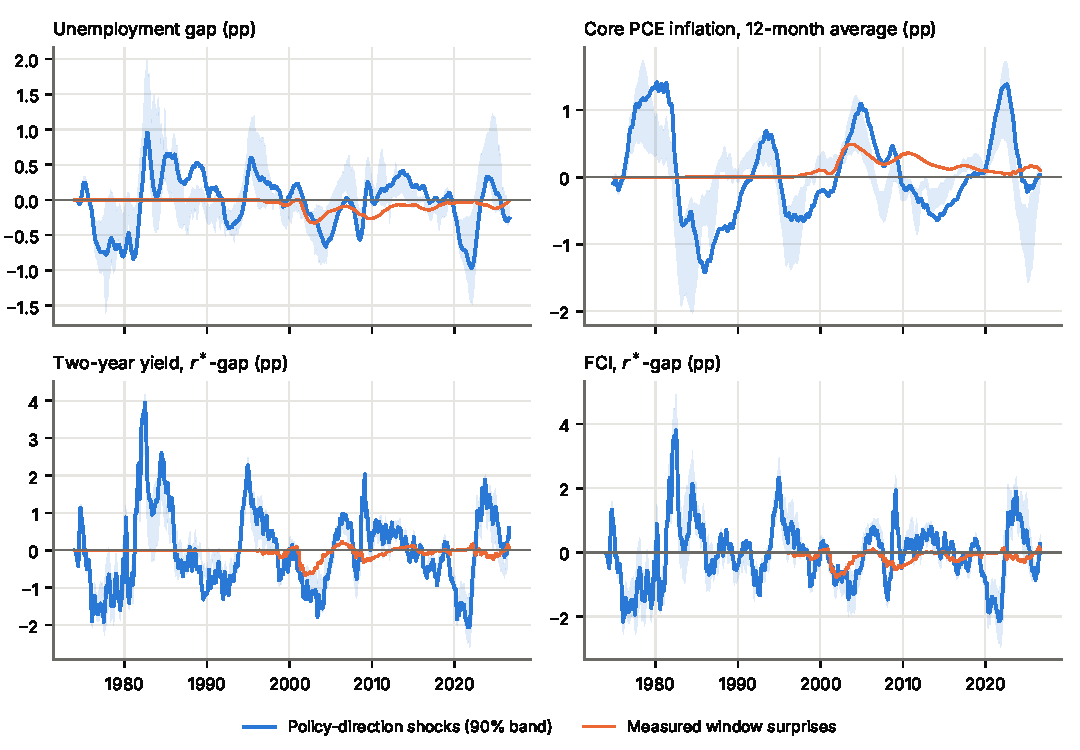
\includegraphics[width=\textwidth]{../baseline/report/fig_decomp_hd.pdf}
\caption{Contributions of Policy-Direction Shocks, 1974--2026}
\label{fig:decomphd}
\begin{flushleft}\footnotesize\textit{Notes:} Historical contributions of policy-direction shocks to the unemployment gap, core PCE inflation (12-month average), the two-year yield and the FCI, all relative to $\rs$, propagated through the model with monthly equations from 1973 (12 lags, March--December 2020 dropped from estimation; the 2020 shocks are decomposed with the estimated coefficients). Orange: the contributions of the measured window surprises. Band: 90 percent interval from the bootstrap draws of the model's responses.\end{flushleft}
\end{figure}

\begin{table}[tp]\centering\small
\caption{How Much Policy Shocks Explain: Variance Shares at 24 Months}\label{tab:decompshares}
\resizebox{\ifdim\width>\textwidth\textwidth\else\width\fi}{!}{%
\begin{tabular}{lcccc}\toprule & \multicolumn{2}{c}{Model from 1996} & \multicolumn{2}{c}{Model from 1973}\\ \cmidrule(lr){2-3}\cmidrule(lr){4-5} Shocks & Unemployment gap & Core inflation & Unemployment gap & Core inflation\\ \midrule
Measured window surprises, 1996--2026 & 0.9 & 0.4 & 0.4 & 0.4\\
 & {\scriptsize [0.2, 1.9]} & {\scriptsize [0.2, 0.9]} & {\scriptsize [0.1, 0.9]} & {\scriptsize [0.1, 0.6]}\\
Policy-direction shocks, 1990--2026 & 18.0 & 9.4 & 8.9 & 7.8\\
 & {\scriptsize [3.5, 39.5]} & {\scriptsize [3.9, 17.5]} & {\scriptsize [1.9, 17.1]} & {\scriptsize [2.5, 12.0]}\\
\quad of which on days without an announcement & 19.2 & 9.4 & 9.5 & 8.3\\
 & {\scriptsize [3.8, 41.8]} & {\scriptsize [3.6, 18.2]} & {\scriptsize [2.1, 18.3]} & {\scriptsize [2.6, 12.8]}\\
Policy-direction shocks, 1974--1989 & 23.7 & 11.4 & 11.8 & 10.1\\
 & {\scriptsize [4.7, 52.0]} & {\scriptsize [6.0, 23.7]} & {\scriptsize [2.6, 22.6]} & {\scriptsize [3.6, 15.8]}\\
\bottomrule\end{tabular}}
\begin{flushleft}\footnotesize\textit{Notes:} Percent of the 24-month forecast-error variance (monthly VAR in monthly averages from 1973, 12 lags) accounted for by the contributions of the shocks of the last 24 months, propagated through the $r^*$-gap model with the FCI (12 lags, March--December 2020 dropped) with monthly equations from 1996 or from 1973; shares over the stated period, March--December 2020 excluded. Measured window surprises: the 252 announcements. Policy-direction shocks: the daily movement of the two-year yield and the FCI in the direction of the window response, recovered from the daily block on every day from 1990; before 1990 from the monthly VAR, scaled to the daily shocks' size. Brackets: 90\% bootstrap bands of Note B's responses.\end{flushleft}
\end{table}


The history the shocks trace is the familiar one (Figure~\ref{fig:decomphd}). Policy-direction shocks eased in 1979--80, lowering unemployment and adding \bl{dc:hist:e7980:pi} percentage point to core inflation on average over those two years. They tightened in 1982--84, raising the two-year yield by \bl{dc:hist:e8284:pol} percentage points and lowering inflation. They eased in 2001--03 and again in 2020--21, when the easing of the yield and the FCI added about \bl{dc:hist:pi2122} percentage point to core inflation in 2021--22. And they tightened in 2022--24. The measured surprises, in orange, are a small part of each episode. The identifying assumption is that within a day the policy shock is recoverable from the innovations of the yield and the FCI; on days without an announcement the shock includes any news that moves the two in the window proportion. Appendix Table~\ref{tab:decompfull} gives every source and horizon, the results with the 2020 shocks absorbed by the month dummies and with the shocks before 1990 unscaled, and Appendix~\ref{app:relation} shows why the shock cannot be recovered from monthly innovations alone.

\FloatBarrier
% ============================================================
\section{Tests of the Approach}\label{sec:tests}
The baseline rests on three choices the data can check: one index, with one set of weights, in place of its three components, the persistence of the financial movement implied by the daily block, and an impact measured in the window rather than estimated from monthly data. The literature offers two other explanations of the puzzles, credit spreads and the averaging of daily data into months, and this section tests both.

\subsection{Which Financial Variables Carry the Response}\label{sec:components}
The baseline assumes that the 10-year yield, equity valuation and the dollar affect unemployment and prices in proportion to the weights with which they respond to policy news. That is an assumption about the economy, and it can be relaxed and tested. I compare three specifications of the monthly equations. In the first the FCI enters as one variable. In the second equities enter separately and the 10-year yield and the dollar enter as one variable. In the third all three enter separately. The daily block is the same in all three, so the specifications differ only in the monthly equations and share their bootstrap draws (Appendix~\ref{app:details}).

\begin{table}[tp]\centering\scriptsize\setlength{\tabcolsep}{3pt}
\caption{Price and Unemployment Responses with the Components Entered Separately}\label{tab:components}
\resizebox{\textwidth}{!}{%
\begin{tabular}{llcccccc}\toprule
 & & \multicolumn{4}{c}{Monthly equations with} & \multicolumn{2}{c}{Difference from the index}\\ \cmidrule(lr){3-6}\cmidrule(lr){7-8}
Start & Response & Index (baseline) & Index, three-component daily block & Equities free & All three free & Equities free & All three free\\ \midrule
1996 & Price level, 24 m (\%) & $-$0.69$^{**}$ & $-$0.66$^{**}$ & $-$0.40 & $-$0.07 & 0.26 & 0.58$^{**}$\\
 & & {\scriptsize [$-$1.08, $-$0.21]} & {\scriptsize [$-$1.04, $-$0.21]} & {\scriptsize [$-$0.78, 0.03]} & {\scriptsize [$-$0.40, 0.40]} & {\scriptsize [$-$0.06, 0.50]} & {\scriptsize [0.24, 0.98]}\\
1996 & Unemployment gap, 24 m (pp) & 0.45$^{**}$ & 0.45$^{**}$ & 0.40$^{*}$ & 0.33 & $-$0.06 & $-$0.12\\
 & & {\scriptsize [0.09, 0.78]} & {\scriptsize [0.11, 0.71]} & {\scriptsize [0.06, 0.69]} & {\scriptsize [$-$0.04, 0.59]} & {\scriptsize [$-$0.28, 0.18]} & {\scriptsize [$-$0.43, 0.14]}\\
\addlinespace
1973 & Price level, 24 m (\%) & $-$0.76$^{**}$ & $-$0.69$^{**}$ & $-$0.54 & $-$0.57 & 0.15 & 0.11\\
 & & {\scriptsize [$-$0.93, $-$0.36]} & {\scriptsize [$-$0.93, $-$0.21]} & {\scriptsize [$-$0.85, 0.00]} & {\scriptsize [$-$0.90, 0.04]} & {\scriptsize [$-$0.14, 0.46]} & {\scriptsize [$-$0.21, 0.54]}\\
1973 & Unemployment gap, 24 m (pp) & 0.24 & 0.44$^{**}$ & 0.11 & 0.08 & $-$0.34$^{**}$ & $-$0.37$^{**}$\\
 & & {\scriptsize [$-$0.02, 0.40]} & {\scriptsize [0.11, 0.64]} & {\scriptsize [$-$0.28, 0.39]} & {\scriptsize [$-$0.31, 0.39]} & {\scriptsize [$-$0.66, $-$0.06]} & {\scriptsize [$-$0.70, $-$0.06]}\\
\bottomrule\end{tabular}
}
\begin{flushleft}\footnotesize\textit{Notes:} $r^*$-gap yield and FCI, 12 lags, per +1 pp on the two-year yield in the window. The last three columns share one daily block (the three components and the two-year yield), so they differ only in the monthly equations: the FCI built from the components as one variable, equities separate with the 10-year yield and the dollar as one variable, or all three separate. The difference columns are computed on common bootstrap draws. The first column is the baseline model with its own daily block. Brackets: 90\% intervals; $^{**}$, $^{*}$: 5 and 10 percent levels. Nominal and real versions: Appendix Table~\ref{tab:appR4c}.\end{flushleft}
\end{table}


In the sample since 1996 the unemployment response barely depends on the specification: after 24 months it is \bl{cp:1996:R:u} percentage point with the index as one variable, \bl{cp:1996:E:u} with equities free and \bl{cp:1996:F:u} with all three free (Table~\ref{tab:components}). The price response does depend on it. Freeing equities leaves most of it in place (\bl{cp:1996:E:P} percent after 24 months, against \bl{cp:1996:R:P} with the index as one variable). Freeing the dollar as well removes it (\bl{cp:1996:F:P}). The coefficients show why. In the inflation equation a tighter 10-year yield lowers inflation, as the baseline assumes, and a tighter dollar, holding the yield and equities fixed, has a conditional effect of the opposite sign (\bl{cp:coef:96:pi:y10} for the yield and \bl{cp:coef:96:pi:usd} for the dollar). A conditional coefficient of this kind does not identify the effect of an exogenous change in the dollar, because the dollar moves with the yield and with equities. It does show that the price result needs the two to enter in proportion.

The formal tests point the same way (Appendix Table~\ref{tab:weightstest}). Equality of the yield and dollar coefficients, with equities free, is rejected in the inflation equation from 1996 in the nominal and real versions and not in the unemployment equation. In the sample from 1973 the three specifications give similar price responses (\bl{cp:1973:R:P}, \bl{cp:1973:E:P} and \bl{cp:1973:F:P}), and the yield-dollar restriction is not rejected. There the specification matters for unemployment instead: with the index built from the components unemployment rises \bl{cp:1973:R:u} percentage point after 24 months, and with equities free about \bl{cp:1973:E:u}, and the test of tying equities to the yield and the dollar rejects in the unemployment equation. In the longer sample, then, the restriction that helps the unemployment response is the one on equities, and in the shorter sample the restriction that helps the price response is the one on the dollar. A stronger dollar lowers import prices, so a dollar channel should lower inflation, and the baseline imposes that it does so in proportion to the yield.\footnote{In the sample from 1996 the data do not support the proportion in the inflation equation; the estimate is imprecise because the sample is short and the dollar's movements are few. A split of core inflation into goods and services would show where the dollar acts.} Both restrictions are those of the index: each asset enters with the weight of its response to policy news.

\subsection{Four Calibrations of the Weights}\label{sec:weights4}
The weights of the index come from one estimate of how the three asset prices respond to policy news. The companion paper shows that other calibrations of the same three assets value their movements differently \citep{fcinote}. Market weights estimated with the two-year yield as the policy signal, and FRB/US funds-rate equivalents, give the dollar more than twice the importance relative to equities that the baseline does; the published Goldman Sachs weights value the two almost as the baseline does. If the result depended on that relative importance, the paper would be about one index rather than about financial conditions. I therefore change only the weights. Each calibration is applied to the same $\rs$-gap series, announcements, dynamics and bootstrap draws, and each is scaled so that its window loading is one, as for the baseline; each gets its own ordinary-day loading (Table~\ref{tab:weights4}).

\begin{table}[tp]\centering\small
\caption{Four Calibrations of the Index Weights ($r^*$-Gap Yield and FCI; 12 Lags)}\label{tab:weights4}
\resizebox{\ifdim\width>\textwidth\textwidth\else\width\fi}{!}{%
\begin{tabular}{lcccccc}\toprule & Dollar relative & Window & Ordinary-day & \multicolumn{2}{c}{Yield and FCI, 24 m} & Shift in unemployment\\ \cmidrule(lr){5-6}
Weights & to equities & loading & loading & Unemployment & Price level & from adding the FCI, 24 m\\ \midrule
Market, futures factor (baseline) & 0.99 & 1.00 & 0.29 & 0.45$^{**}$ & $-$0.69$^{**}$ & 0.66 [0.27, 1.00]\\
Market, two-year yield & 2.06 & 1.00 & 0.66 & 0.18 & $-$0.44$^{*}$ & 0.40 [0.10, 0.66]\\
FRB/US & 2.51 & 1.00 & 0.38 & 0.09 & $-$0.39 & 0.30 [$-$0.02, 0.58]\\
Goldman Sachs, published & 0.96 & 1.00 & 0.19 & 0.46$^{**}$ & $-$0.72$^{**}$ & 0.67 [0.27, 1.03]\\
\bottomrule\end{tabular}}
\begin{flushleft}\footnotesize\textit{Notes:} Per +1 pp on the two-year yield in the announcement window, 1996--2026. Each row builds the index from the same three $r^*$-gap series with the weights of one calibration in the companion paper \citep{fcinote}: market weights estimated with the futures factor or the two-year yield as the policy signal, FRB/US funds-rate equivalents, and the published Goldman Sachs weights; each is scaled so that its window loading is one. Dollar relative to equities: the weight on a 3.9 percent dollar appreciation relative to that on a 5 percent fall in stock valuations. Ordinary-day loading: the FCI movement that accompanies a 1 pp rise in the yield on days without an announcement. Shift: the response with the FCI minus the response with the yield alone (same draws), with its 90 percent interval. $^{**}$ and $^{*}$: the 95 and 90 percent intervals exclude zero.\end{flushleft}
\end{table}


The result holds under every calibration, and the four agree closely on its size. From 1973 the price level falls \bl{rv:w4m:73:P24:minabs} to \bl{rv:w4m:73:P24:maxabs} percent after two years under the four weightings, and unemployment rises \bl{rv:w4m:73:u12:min} to \bl{rv:w4m:73:u12:max} percentage point after one year. From 1996 the futures-factor and the published Goldman Sachs weightings give nearly identical responses (\bl{rv:w4:F:u} and \bl{rv:w4:G:u} percentage point for unemployment and \bl{rv:w4:F:P} and \bl{rv:w4:G:P} percent for prices after 24 months), and the other two give smaller ones. Adding financial conditions raises the two-year unemployment response by \bl{rv:w4:shmin} to \bl{rv:w4:shmax} percentage point. All four have a window loading of one; what differs is the ordinary-day loading and the propagation. The market weights with the two-year yield and the FRB/US weights put more weight on assets that move with the two-year yield on ordinary days as well; their ordinary-day loadings are \bl{rv:w4:Y:ord} and \bl{rv:w4:B:ord}, the gap to the window is smaller, and so are their shifts in unemployment. The finding is about the bundle of financial prices that moves with policy news, not about one weighting of it.

\subsection{How Long Does the Financial Movement Last?}\label{sec:resolve}
In the window the FCI moves one for one with the yield. After the window, the daily block decides how long the movement lasts, and that matters because the monthly equations respond to monthly averages. Figure~\ref{fig:financial} shows the responses of the yield and the FCI in the baseline.

The days after announcements offer a check on that persistence. I measure the change in each series at 5, 22 and 66 trading days after each announcement, and its average over the first 22 days, on the same clock as the model (Appendix~\ref{app:persist}). For the yield the direct estimates agree with the model at every horizon. For the FCI they agree at 5 and 22 days and have little power at 66 days, where the interval runs from a complete reversal to more than the model's value (Figure~\ref{fig:persist}). The first-month average of the FCI is higher in the data than in the model when measured from the window, because part of the window's movement reverses by the close, and about the same when measured from the close before the announcement; neither difference changes the responses. Persistence beyond the first month would matter: a shorter FCI path would lower the baseline unemployment response after 24 months from \bl{pe:rho:base:u24} to \bl{pe:rho:pt:u24}. The model's persistence is consistent with the data, which cannot distinguish it from that shorter path.

\begin{figure}[tp]
\centering
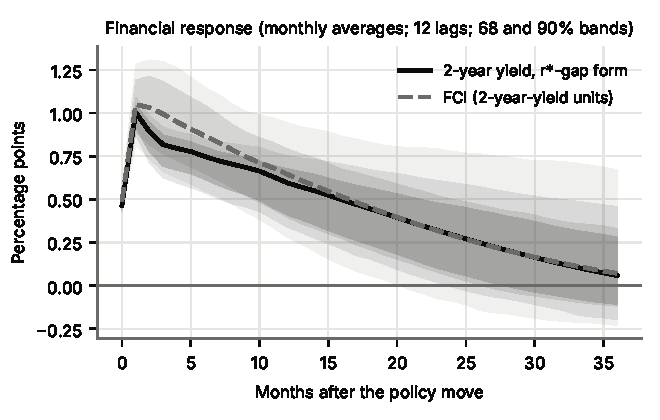
\includegraphics[width=0.62\textwidth]{../baseline/report/fig_financial.pdf}
\caption{Response of the Two-Year Yield and the FCI to a Policy Move}
\label{fig:financial}
\begin{flushleft}\footnotesize\textit{Notes:} The FCI is measured relative to $\rs$ and in two-year-yield units; the policy move raises the two-year yield 1 percentage point in the window. Monthly averages; 12 lags; 68 and 90 percent bands.\end{flushleft}
\end{figure}

\begin{figure}[tp]
\centering
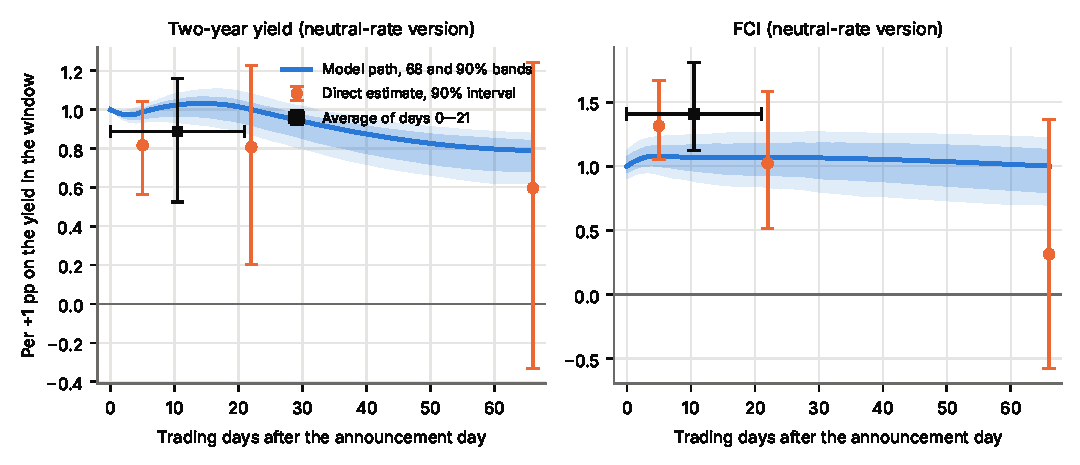
\includegraphics[width=\textwidth]{../baseline/report/fig_persist.pdf}
\caption{Financial Persistence: Direct Estimates and the Model}
\label{fig:persist}
\begin{flushleft}\footnotesize\textit{Notes:} Per +1 pp on the two-year yield in the window, $r^*$-gap versions. Blue: the model's daily path after the announcement day (day 0), with 68 and 90 percent bands. Orange: direct estimates at 5, 22 and 66 trading days with 90 percent intervals. Black square: the average of days 0 to 21, with its interval; the horizontal bar shows the days averaged. The calendar-month averages of Figure~\ref{fig:financial} measure something different.\end{flushleft}
\end{figure}

\subsection{Monthly Benchmarks}\label{sec:monthlyvar}
Could a standard monthly model with the FCI added do the same job? A valid external instrument can recover the total response with the transmission channels unobserved, so a yield-only model is not wrong by construction; the question is what works in these data. I estimate two monthly VARs with the yield and the FCI relative to $\rs$. A proxy VAR estimates the immediate effect of the surprise on every variable from monthly residuals and the instrument. A window-impact VAR takes the effect on the yield and the FCI from the windows, as the main model does, and sets the effect on unemployment and inflation to zero within the month; it has no daily block, so the timing of announcements within the month is lost.

\begin{table}[tp]\centering\small
\caption{Monthly VARs with the FCI and the Main Model ($r^*$-gap Two-Year Yield and FCI; 12 Lags)}\label{tab:monthlycompact}
\resizebox{\ifdim\width>\textwidth\textwidth\else\width\fi}{!}{%
\begin{tabular}{lrrrr}\toprule & \multicolumn{2}{c}{Unemployment gap (pp)} & \multicolumn{2}{c}{Price level (\%)}\\ \cmidrule(lr){2-3}\cmidrule(lr){4-5} & 12 m & 24 m & 12 m & 24 m\\ \midrule
Proxy VAR & $-$0.03 & $-$0.15 & $-$0.36 & $-$0.51\\
 & {\scriptsize [$-$1.32, 2.46]} & {\scriptsize [$-$1.74, 1.75]} & {\scriptsize [$-$5.90, 0.18]} & {\scriptsize [$-$8.47, 0.27]}\\
Window-impact VAR & 0.22$^{*}$ & 0.13 & $-$0.17$^{*}$ & $-$0.30$^{*}$\\
 & {\scriptsize [0.01, 0.35]} & {\scriptsize [$-$0.09, 0.30]} & {\scriptsize [$-$0.26, $-$0.04]} & {\scriptsize [$-$0.46, $-$0.06]}\\
Main model (daily block) & 0.41$^{*}$ & 0.45$^{*}$ & $-$0.38$^{*}$ & $-$0.69$^{*}$\\
 & {\scriptsize [0.16, 0.60]} & {\scriptsize [0.09, 0.78]} & {\scriptsize [$-$0.55, $-$0.16]} & {\scriptsize [$-$1.08, $-$0.21]}\\
\bottomrule\end{tabular}}
\begin{flushleft}\footnotesize\textit{Notes:} Per +1 pp on the two-year yield. $^{*}$: the 90\% interval excludes zero; intervals in brackets (Anderson--Rubin sets for the proxy VAR; bootstrap for the others). Monthly VARs use monthly averages; unit +1 pp on the two-year yield in the announcement window.\end{flushleft}
\end{table}


Both give the signs of the main model at a smaller size (Table~\ref{tab:monthlycompact}). The window-impact VAR gives unemployment \bl{mo:rstar:yes:WE:u:12} percentage point higher after 12 months and the price level \blabs{mo:rstar:yes:WE:P:24} percent lower after 24, about half the main model's \bl{rstar:yes:u:12} and \blabs{rstar:yes:P:24}; from 1973 it gives \bl{mo73:rstar:yes:WE:u:12} and \blabs{mo73:rstar:yes:WE:P:24}. The proxy VAR has wide sets, because the surprise is a weak instrument for monthly residuals (first-stage $F$ of \bl{mo:rstar:yes:F} from 1996 and \bl{mo73:rstar:yes:F} from 1973). The smaller size is what monthly averaging does. A window move of 1 percentage point raises the month's average yield by only \bl{mo:win}, and a monthly VAR cannot reproduce the rest of the movement, which arrives the next month. A simulation with the baseline model as the true process confirms this: the window-impact VAR recovers about half the true unemployment response at 12 months (median \bl{sim:window:u12:med} against \bl{sim:window:u12:truth}) with a narrow range, the proxy VAR with the FCI is centred below the truth with a range that runs from \bl{sim:proxy_fci:u12:lo} to \bl{sim:proxy_fci:u12:hi}, and the proxy VAR without the FCI is centred near zero (Appendix Table~\ref{tab:proxysim}). Tracking the daily path of the financial movement, as the main model does, is what recovers the full response \citep{jacobson2026}.

A direct projection of each outcome on the surprise imposes no channel at all (Appendix~\ref{app:direct}). With lags of unemployment and inflation as the only controls it gives large wrong-signed estimates: unemployment \bl{dp:m:u:12} percentage point after 12 months. Adding lags of the yield and the FCI shrinks the estimates toward zero (\bl{dp:f:u:12}), and no interval then excludes zero. The surprise by itself does not pin down the macroeconomic response. A model of financial propagation, or at least the monthly dynamics of a VAR, is needed for an informative estimate.

\subsection{Credit Spreads}\label{sec:credit}
Credit is the most important channel the baseline leaves out \citep{gertler2015,gilchrist2012,caldara2019}. If a credit premium that responds to policy carried part of what the FCI carries, the FCI would take credit for effects that belong to credit. I test this in two ways (Table~\ref{tab:credit}). First, the monthly excess bond premium of \citet{gilchrist2012} enters as a third monthly variable, set within the month before markets like unemployment and inflation. Second, the daily Baa corporate spread over the 10-year Treasury enters the daily block next to the yield and the FCI. It has no intraday series, so its impact is its change on the announcement day, \bl{rv:cr:baaimp} percentage point per percentage point on the yield: the 10-year yield rises on the day by more than the Baa yield.

\begin{table}[tp]\centering\small
\caption{Credit and the Response ($r^*$-Gap Yield; 12 Lags)}\label{tab:credit}
\resizebox{\ifdim\width>\textwidth\textwidth\else\width\fi}{!}{%
\begin{tabular}{lcccc}\toprule & Yield alone & \multicolumn{2}{c}{Yield and FCI} & Credit measure \\ \cmidrule(lr){2-2}\cmidrule(lr){3-4}\cmidrule(lr){5-5}
 & Unemployment, 24 m & Unemployment, 24 m & Price level, 24 m & Response, 12 m (pp)\\ \midrule
Baseline & $-$0.21 & 0.45$^{**}$ & $-$0.69$^{**}$ & --\\
Excess bond premium in the monthly block & 0.06 & 0.44$^{*}$ & $-$0.59$^{**}$ & $-$0.01 [$-$0.22, 0.13]\\
Baa spread in the daily block & $-$0.21 & 0.34 & $-$0.60$^{*}$ & $-$0.09 [$-$0.24, 0.09]\\
\bottomrule\end{tabular}}
\begin{flushleft}\footnotesize\textit{Notes:} Per +1 pp on the two-year yield in the announcement window, 1996--2026. Excess bond premium: a third monthly variable, set like unemployment and inflation before markets within the month. Baa spread: Moody's Baa yield less the 10-year Treasury yield, in the daily block next to the yield and the FCI; its impact is its announcement-day change, because it has no intraday series. In the Baa row the yield-alone entry is the baseline's. Credit response: the excess bond premium, or the monthly average of the Baa spread, 12 months after the move, with its 90 percent interval. $^{**}$ and $^{*}$: the 95 and 90 percent intervals exclude zero.\end{flushleft}
\end{table}


Neither credit measure changes the result. With the excess bond premium, unemployment rises \bl{rv:cr:E:u} percentage point after 24 months and the price level falls \blabs{rv:cr:E:P} percent, against \bl{rv:cr:B:u} and \blabs{rv:cr:B:P} in the baseline. With the daily spread they are \bl{rv:cr:A:u} and \blabs{rv:cr:A:P}; the unemployment response is smaller and its interval includes zero, and the price response is significant. The credit measures themselves move little after a tightening once the FCI is in the model: the response of the excess bond premium after 12 months is \bl{rv:cr:ebp12} percentage point, with an interval that includes zero. The index already contains much of what moves credit premia. The three components of the index account for \bl{rv:cr:r2d} percent of the variation in three-month changes of the excess bond premium since 1996, and equities alone for \bl{rv:cr:r2eq} percent, consistent with risk appetite moving both \citep{bauer2026}. Without the FCI, adding the excess bond premium moves the unemployment response toward zero, in the direction that adding the FCI moves it, because the premium then stands in for part of the channel. The three-variable index captures the risk-taking channel through the prices that reveal it in the announcement window.

\subsection{Temporal Aggregation and Financial Conditions}\label{sec:timingtest}
\citet{jacobson2026} show that averaging daily data into months biases the estimated effects of policy, because a surprise late in a month barely affects that month's average while one early in the month affects most of it. My model tracks when in the month each announcement falls; the window-impact monthly VAR of Section~\ref{sec:monthlyvar} does not. Comparing the two, with and without the FCI, separates the two corrections (Table~\ref{tab:timing2}).

\begin{table}[tp]\centering\small
\caption{Two Corrections: Announcement Timing and Financial Conditions (24 Months; 12 Lags)}\label{tab:timing2}
\resizebox{\ifdim\width>\textwidth\textwidth\else\width\fi}{!}{%
\begin{tabular}{llcccc}\toprule & & \multicolumn{2}{c}{Yield alone} & \multicolumn{2}{c}{Yield and FCI}\\ \cmidrule(lr){3-4}\cmidrule(lr){5-6}
Yield & Response & Monthly VAR & Daily block & Monthly VAR & Daily block\\ \midrule
Nominal & Unemployment gap (pp) & $-$0.33$^{*}$ & $-$0.45$^{**}$ & 0.01 & 0.16\\
 & Price level (\%) & 0.04 & 0.06 & $-$0.14 & $-$0.29\\\addlinespace
Real & Unemployment gap (pp) & $-$0.26$^{*}$ & $-$0.35$^{**}$ & 0.04 & 0.23$^{*}$\\
 & Price level (\%) & $-$0.04 & $-$0.06 & $-$0.20 & $-$0.38$^{**}$\\\addlinespace
$r^*$-gap & Unemployment gap (pp) & $-$0.13 & $-$0.21 & 0.13 & 0.45$^{**}$\\
 & Price level (\%) & $-$0.17 & $-$0.32 & $-$0.30$^{*}$ & $-$0.69$^{**}$\\
\bottomrule\end{tabular}}
\begin{flushleft}\footnotesize\textit{Notes:} Per +1 pp on the two-year yield in the announcement window, 1996--2026. Monthly VAR: the window-impact monthly VAR of Section~\ref{sec:monthlyvar}, which takes the impact from the windows and treats every announcement as if it fell at the start of its month (end-of-month series). Daily block: the main model, which tracks when in the month each announcement falls. $^{**}$ and $^{*}$: the 95 and 90 percent intervals exclude zero.\end{flushleft}
\end{table}


Both corrections raise the unemployment response, and they compound. With the yield alone, neither model gives a rise in unemployment, whether the timing is tracked or not. Adding the FCI raises the unemployment response after 24 months in every version, by \bl{rv:tm:nom:u:fci}, \bl{rv:tm:real:u:fci} and \bl{rv:tm:rstar:u:fci} percentage point on average across the two models for the nominal, real and $\rs$-gap yields. Tracking the timing adds \bl{rv:tm:nom:u:timefci}, \bl{rv:tm:real:u:timefci} and \bl{rv:tm:rstar:u:timefci} once the FCI is in the model, and \bl{rv:tm:nom:u:timeno}, \bl{rv:tm:real:u:timeno} and \bl{rv:tm:rstar:u:timeno} without it. Timing matters most when the financial movement it times is large. Omitted financial channels and temporal aggregation are thus two sources of the puzzle, and the financial channel is the larger one. \citet{jacobson2026} correct the second with a daily price index; this paper corrects the first with standard monthly data on core prices and unemployment.

\FloatBarrier
% ============================================================
\section{Robustness}\label{sec:rob}
A result about the transmission of monetary policy can rest on one sample, one estimate of $\rs$, one trend, one set of omitted variables, one surprise series or one lag length. I vary each in turn, changing one feature of the baseline and keeping the rest, in both samples (Table~\ref{tab:robsummary}). The table reports the responses of the $\rs$-gap model with the FCI after 12 months, where both responses are well measured in both samples; the appendix gives 12, 24 and 36 months for every version and test.

\begin{table}[tp]\centering\small
\caption{Robustness: Responses at 12 Months}\label{tab:robsummary}
\resizebox{\ifdim\width>\textwidth\textwidth\else\width\fi}{!}{%
\begin{tabular}{lcccc}\toprule & \multicolumn{2}{c}{Monthly equations from 1996} & \multicolumn{2}{c}{Monthly equations from 1973}\\ \cmidrule(lr){2-3}\cmidrule(lr){4-5} & Unemployment gap & Price level & Unemployment gap & Price level\\ \midrule
Baseline & 0.41$^{**}$ & $-$0.38$^{**}$ & 0.33$^{**}$ & $-$0.32$^{**}$\\
 & {\scriptsize [0.16, 0.60]} & {\scriptsize [$-$0.55, $-$0.16]} & {\scriptsize [0.14, 0.46]} & {\scriptsize [$-$0.42, $-$0.16]}\\
\midrule
2020 left in & 0.33 & $-$0.42$^{**}$ & 0.18 & $-$0.27$^{**}$\\
 & {\scriptsize [$-$0.06, 0.76]} & {\scriptsize [$-$0.60, $-$0.20]} & {\scriptsize [$-$0.07, 0.38]} & {\scriptsize [$-$0.41, $-$0.10]}\\
Kiley $r^*$ & 0.10 & $-$0.14 & 0.14 & $-$0.26$^{**}$\\
 & {\scriptsize [$-$0.08, 0.30]} & {\scriptsize [$-$0.31, 0.01]} & {\scriptsize [0.00, 0.24]} & {\scriptsize [$-$0.35, $-$0.15]}\\
Real yield and FCI, spline trend (no $r^*$) & 0.18 & $-$0.15 & 0.29$^{**}$ & $-$0.21$^{**}$\\
 & {\scriptsize [$-$0.05, 0.31]} & {\scriptsize [$-$0.31, 0.07]} & {\scriptsize [0.13, 0.41]} & {\scriptsize [$-$0.30, $-$0.08]}\\
Excess bond premium added & 0.39$^{**}$ & $-$0.33$^{**}$ & 0.22$^{**}$ & $-$0.31$^{**}$\\
 & {\scriptsize [0.17, 0.54]} & {\scriptsize [$-$0.47, $-$0.12]} & {\scriptsize [0.08, 0.33]} & {\scriptsize [$-$0.41, $-$0.15]}\\
FCI components, equities free & 0.35$^{**}$ & $-$0.26$^{**}$ & 0.32$^{**}$ & $-$0.30$^{**}$\\
 & {\scriptsize [0.11, 0.50]} & {\scriptsize [$-$0.41, $-$0.05]} & {\scriptsize [0.15, 0.42]} & {\scriptsize [$-$0.39, $-$0.16]}\\
Bauer--Swanson surprise & 0.46$^{**}$ & $-$0.39$^{**}$ & 0.36$^{**}$ & $-$0.33$^{**}$\\
 & {\scriptsize [0.19, 0.67]} & {\scriptsize [$-$0.57, $-$0.16]} & {\scriptsize [0.16, 0.50]} & {\scriptsize [$-$0.43, $-$0.15]}\\
3 lags & 0.37$^{**}$ & $-$0.22 & 0.12 & $-$0.09\\
 & {\scriptsize [0.14, 0.57]} & {\scriptsize [$-$0.42, 0.01]} & {\scriptsize [$-$0.02, 0.18]} & {\scriptsize [$-$0.16, 0.16]}\\
6 lags & 0.38$^{**}$ & $-$0.30$^{**}$ & 0.27$^{**}$ & $-$0.20$^{*}$\\
 & {\scriptsize [0.15, 0.56]} & {\scriptsize [$-$0.45, $-$0.08]} & {\scriptsize [0.10, 0.35]} & {\scriptsize [$-$0.31, $-$0.01]}\\
Industrial production added & 0.37$^{**}$ & $-$0.43$^{**}$ & 0.33$^{**}$ & $-$0.28$^{**}$\\
 & {\scriptsize [0.11, 0.55]} & {\scriptsize [$-$0.59, $-$0.18]} & {\scriptsize [0.13, 0.45]} & {\scriptsize [$-$0.40, $-$0.11]}\\
Federal funds rate in the daily block & 0.43$^{**}$ & $-$0.42$^{**}$ & 0.31$^{**}$ & $-$0.38$^{**}$\\
 & {\scriptsize [0.17, 0.61]} & {\scriptsize [$-$0.58, $-$0.19]} & {\scriptsize [0.13, 0.48]} & {\scriptsize [$-$0.48, $-$0.19]}\\
\bottomrule\end{tabular}}
\begin{flushleft}\footnotesize\textit{Notes:} $r^*$-gap two-year yield and FCI; responses 12 months after a policy move that raises the two-year yield 1 percentage point in the announcement window; unemployment gap in percentage points, price level in percent; 12 lags unless stated; March--December 2020 dropped unless stated. $^{**}$ and $^{*}$: the 95\% and 90\% bootstrap intervals exclude zero; 90\% intervals in brackets. The tests are described in Section 5; full results at 12, 24 and 36 months for every version are in the appendix.\end{flushleft}
\end{table}


The responses are stable. From 1996, eight of the ten tests give unemployment \bl{rob:mid:u:lo} to \bl{rob:mid:u:hi} percentage point higher and the price level \bl{rob:mid:P:lo} to \bl{rob:mid:P:hi} percent lower after a year, around the baseline's \bl{rstar:yes:u:12} and \blabs{rstar:yes:P:12}. The two that differ both change the treatment of $\rs$: Kiley's estimate gives \bl{rob:kiley:u:abs} and \bl{rob:kiley:P:abs}, and the real yield with a spline trend \bl{rob:spline:u:abs} and \bl{rob:spline:P:abs}. From 1973 the responses are a little smaller and as uniform: eight of the ten tests give \bl{rob:mid73:u:lo} to \bl{rob:mid73:u:hi} percentage point and \bl{rob:mid73:P:lo} to \bl{rob:mid73:P:hi} percent, around the baseline's \bl{b73:rstar:yes:u:12} and \blabs{b73:rstar:yes:P:12}. With 3 lags both responses are smaller (\bl{rob:L373:u:abs} and \bl{rob:L373:P:abs}), and Kiley's $\rs$ gives a smaller rise in unemployment (\bl{rob:kiley73:u:abs}) with the usual fall in prices (\bl{rob:kiley73:P:abs}). In every test, from both starting dates, a tightening raises unemployment and lowers prices after a year, and the baseline responses are significant at the 5 percent level in both samples.

\subsection{The Sample}\label{sec:recent}
The sample since 1996 is short, it contains the pandemic, when unemployment moved by more than in any other period, and it ends with the largest tightening in the sample. Keeping March to December 2020 in the estimation leaves the responses close to the baseline (\bl{rob:t2020:u:abs} and \bl{rob:t2020:P:abs} after a year from 1996) with wider intervals. Ending all equations in December 2019 weakens the price response from 1996, from \bl{sm:base96:P:24} to \bl{sm:end96:P:24} percent after two years; from 1973 it is \bl{sm:end73:P:24}, close to the baseline. Core inflation varied little before 2020 (a standard deviation of \bl{sm:pi:sd:9619} percentage points for 1996--2019, against \bl{sm:pi:sd:2026} for 2020--26 and \bl{sm:pi:sd:7319} for 1973--2019), so the short sample has little information on how inflation responds to financial conditions, and the later years and the earlier decades supply it.

\subsection{The $r^*$ Adjustment and Trends}\label{sec:rstarrob}
The neutral rate is not observed, so the results could be an artifact of the Laubach--Williams estimate. One test replaces it with Kiley's estimate, in the yield and the FCI alike. Another uses no $\rs$ at all: it keeps the real yield and the real FCI and adds a natural cubic spline in time to every monthly equation. From 1996 both give responses of the same sign and a quarter to a half of the baseline's size. From 1973 the price level still falls \bl{rob:kiley73:P:abs} and \bl{rob:spline73:P:abs} percent after a year, against \blabs{b73:rstar:yes:P:12} in the baseline. The measure of $\rs$ matters for the size of the responses since 1996, not for their direction.

\subsection{Credit, the Surprise and Lag Length}\label{sec:surprise}
Adding the excess bond premium as a third monthly variable leaves the responses close to the baseline in both samples (\bl{rob:ebp:u:abs} and \bl{rob:ebp:P:abs} after a year from 1996), as Section~\ref{sec:credit} found at two years. An announcement can reveal the Fed's view of the economy as well as a change in policy, and part of each surprise can be predicted from public data. The orthogonalized surprise of \citet{bauer2023}, which removes the predictable part and is available through 2019 (\bl{ev:bs} announcements), gives responses at least as large as the baseline's (\bl{rob:bs:u:abs} and \bl{rob:bs:P:abs}); the sign restriction of \citet{jarocinski2020} (\bl{ev:jk} announcements) is in the appendix. The baseline uses 12 monthly lags, fixed in advance. With 6 lags the unemployment response from 1996 is close to the baseline and the price fall about a fifth smaller, and both are somewhat smaller from 1973; with 3 lags they keep their signs and are smaller, most of all from 1973 (Appendix~\ref{app:lags}).

\subsection{Further Variables}\label{sec:extensions}
Two tests add a variable the baseline leaves out. Industrial production, as a third monthly variable, leaves the responses of unemployment and prices as in the baseline (\bl{rob:ip:u:abs} and \bl{rob:ip:P:abs} after a year from 1996). The federal funds rate, as a third daily variable that moves on the announcement day with the window change of current-month funds futures, does the same (\bl{rob:ff:u:abs} and \bl{rob:ff:P:abs}), so the two-year yield and the FCI already carry what the policy rate adds. Finally, using the 1-year yield in place of the 2-year gives responses about a quarter larger per percentage point of its own window move, in proportion to its smaller move in the window (\bl{rob:ratio1y} of the two-year's); the responses to a surprise of a given size are about the same (Appendix Table~\ref{tab:mainR7}).

\FloatBarrier
% ============================================================
\section{Conclusion}\label{sec:policy}
Interest-rate surprises around Federal Reserve announcements identify policy shocks well. The difficulty has been tracing their effects. I kept the surprise as it is and changed how its effects are traced: through broad financial conditions measured relative to the neutral rate, rather than through one interest rate. Traced this way, a tightening raises unemployment and lowers prices, where the standard methods give a fall in unemployment and no response of prices.

The difference is in what the surprises move. On announcement days a rise in the two-year yield comes with a tightening of financial conditions \bl{rv:ord:ratio} times as large as on ordinary days, and a model that sees only the yield treats a policy surprise as an ordinary rise in rates. Credit spreads, the timing of announcements within the month and cleaned surprises do not explain the result away.

The results change the measured cost of lowering inflation. A 1 percent lower core price level after two years comes with about one percentage-point year of unemployment, \bl{tr:sac:24} in the sample since 1996 and \bl{tr73:sac:24} in the sample from 1973. That tradeoff is much steeper than earlier high-frequency estimates for the period since 1990 imply, and close to estimates for the decades before.

Policy surprises explain little of the fluctuations in unemployment and inflation, and movements of rates and financial conditions in the direction of policy news explain about a tenth. Those movements trace the familiar history: the easing of 1979--80, the tightening of 1982--84, and the easing of 2020--21 that added about \bl{dc:hist:pi2122} percentage point to core inflation in 2021--22.

The most durable finding is the matched comparison. In the sample since 1996, adding financial conditions raises the two-year unemployment response by about 0.6 percentage point and deepens the price decline by about a third of a percent, whether the yield is nominal, real or relative to the neutral rate; in the longer sample, financial conditions enlarge responses that already have the conventional signs, and the price level falls by about the same amount in both. That policymakers watch financial conditions is familiar. What the paper shows is that estimates of transmission need them: for a given surprise to the expected path of rates, the accompanying movement in long yields, equities and the dollar determines the estimated employment consequences.

\FloatBarrier
\bibliographystyle{aea}
\bibliography{references}

\FloatBarrier
\newpage
\begin{appendices}
\renewcommand{\thetable}{\Alph{section}\arabic{table}}
\renewcommand{\thefigure}{\Alph{section}\arabic{figure}}
\setcounter{table}{0}
\setcounter{figure}{0}
% TODO: Appendix: the 3/6/12-lag tables now come from baseline/. Still to check: the data-sources table and the construction text against baseline/data/SOURCES.md (unverified items: EBP file origin, r* vintage, daily CAPE and dollar file, DFF and PPIACO copies).
\FloatBarrier
% ============================================================
\section{A Two-Equation Illustration}\label{app:toy}
Let $U_t$ be the unemployment gap, $i_t$ the policy rate and $f_t$ financial conditions, with a higher $f_t$ meaning tighter conditions:
\begin{align}
U_t &= \rho_U\,U_{t-1} + \kappa\,f_{t-1} + \varepsilon^{U}_t, \label{eq:y}\\
f_t &= \rho_f\,f_{t-1} + \lambda\,i_t + \varepsilon^{f}_t. \label{eq:f}
\end{align}
Unemployment responds to financial conditions and not directly to the policy rate. Financial conditions respond to the policy rate and to other forces, $\varepsilon^{f}_t$, such as changes in risk appetite. Some of these other forces may themselves be policy news that does not move interest rates \citep{boehm2024,bauer2026}. Suppose the economist observes only $U_t$ and $i_t$. To remove $f_t$, lag equation~\eqref{eq:y} one month, multiply it by $\rho_f$, subtract it from equation~\eqref{eq:y}, and use equation~\eqref{eq:f}. This gives
\begin{equation}
U_t = (\rho_U+\rho_f)\,U_{t-1} - \rho_U\rho_f\,U_{t-2} + \kappa\lambda\,i_{t-1} + \underbrace{\varepsilon^{U}_t - \rho_f\,\varepsilon^{U}_{t-1} + \kappa\,\varepsilon^{f}_{t-1}}_{\text{error}}. \label{eq:reduced}
\end{equation}
The policy rate has no direct effect in this model. It appears in equation~\eqref{eq:reduced} because it stands in for financial conditions. The error is a moving average that includes past financial shocks, so a VAR in $U_t$ and $i_t$ with few lags cannot capture it. The VAR is misspecified. With the lags and samples available in practice, this can make the effects of monetary policy harder to measure.

\FloatBarrier
% ============================================================
\section{Relation to a Monthly VAR and a Proxy VAR}\label{app:relation}
Suppose the daily block were replaced by a monthly equation for $\bar x_t$, and every announcement occurred on the first day of the month. With $Z_t=(m_t',\bar x_t')'$, the model would then be a standard monthly VAR with a recursive ordering, the macroeconomic variables first, and impact vector $(0,0,b')'$. The daily block adds two things: the position of each announcement in its month, and fast dynamics of the financial variables, estimated on many more observations. A proxy VAR \citep{gertler2015,mertens2013,stock2018} instead estimates $Z_t=\sum_l C_l Z_{t-l}+\iota_t$ and uses as an instrument $z_t$ the surprises summed over the month. The effect on the FCI per unit effect on the two-year yield is then
\begin{equation}
\frac{\operatorname{Cov}(\iota_{F,t},z_t)}{\operatorname{Cov}(\iota_{R,t},z_t)}. \label{eq:proxy}
\end{equation}
The window ratio $b_F$ in equation~\eqref{eq:impact} has the same form, with three differences. It replaces monthly VAR residuals with changes measured inside the window, which do not depend on how strongly the surprise predicts monthly residuals. It sets the entries for unemployment and inflation to zero rather than estimating them. And it dates each shock to its day rather than summing shocks over a month. Section~\ref{sec:monthlyvar} estimates both monthly benchmarks, and Table~\ref{tab:proxysim} shows how each performs when the baseline model is the true process. In large samples a VAR of this kind estimates the same effects as local projections \citep{plagborg2021}. In the language of mixed-data sampling, the monthly equation gives equal weights to the days within a month and unrestricted weights to the months \citep{ghysels2007,foroni2015}. All monthly VARs in the paper use monthly averages of the daily series, the same data as the model's monthly equations; a window move of 1 percentage point raises the month's average yield by about \bl{mo:win}, and the rest of the move arrives in the following month, which a monthly VAR does not reproduce.

\textbf{Can a monthly VAR recover the shock?} Recovering a policy shock from monthly innovations requires the shock to be a linear combination of the innovations of the month (invertibility). Table~\ref{tab:decompdiag} checks this in each version. The month's sum of the measured surprises explains at most a few percent of the month's VAR innovations, adding six months of later innovations raises that share little, and the shock recovered from the innovations in the window direction has a low correlation with the surprise. Its implied variance is many times that of the surprise, so it mixes the policy shock with other shocks. The same pattern appears in samples simulated from the model, in which the policy shock is the window surprise by construction. The failure is therefore a property of how a surprise concentrated on one day enters monthly averages, and it is why Section~\ref{sec:shares} recovers policy-direction shocks from the daily block rather than from a monthly VAR.

\begin{table}[tp]\centering\scriptsize
\caption{Can a Monthly VAR Recover the Window Surprise?}\label{tab:decompdiag}
\resizebox{\ifdim\width>\textwidth\textwidth\else\width\fi}{!}{%
\begin{tabular}{lllrrrrr}\toprule Yield & FCI & Start & $R^2$, innovations (\%) & $R^2$, with 6 leads (\%) & $p$, leads & Correlation & Variance ratio\\ \midrule
Nominal & yield alone & 1973 & 2.0 & 15.8 & 0.05 & 0.10 & 100\\
Nominal & with FCI & 1973 & 0.3 & 17.6 & 0.04 & 0.02 & 70\\
Real & yield alone & 1973 & 1.5 & 14.1 & 0.06 & 0.08 & 114\\
Real & with FCI & 1973 & 0.2 & 15.5 & 0.08 & 0.01 & 75\\
$r^*$-gap & yield alone & 1973 & 1.8 & 14.8 & 0.06 & 0.09 & 112\\
$r^*$-gap & with FCI & 1973 & 0.4 & 16.1 & 0.07 & 0.04 & 75\\
Nominal & yield alone & 1996 & 2.6 & 16.2 & 0.08 & 0.16 & 71\\
Nominal & with FCI & 1996 & 0.9 & 18.4 & 0.03 & 0.07 & 49\\
Real & yield alone & 1996 & 2.2 & 14.3 & 0.10 & 0.13 & 80\\
Real & with FCI & 1996 & 0.9 & 16.1 & 0.19 & 0.07 & 50\\
$r^*$-gap & yield alone & 1996 & 2.5 & 15.3 & 0.10 & 0.14 & 80\\
$r^*$-gap & with FCI & 1996 & 1.5 & 17.3 & 0.11 & 0.10 & 50\\
\addlinespace Simulation, model as truth (median [5th, 95th]) & & & 2.2 [0.5, 4.5] & & & 0.10 [0.02, 0.19] & 74\\
\bottomrule\end{tabular}}
\begin{flushleft}\footnotesize\textit{Notes:} Monthly VAR in monthly averages (12 lags, March--December 2020 dropped). $R^2$: the month's sum of the measured surprises regressed on the month's VAR innovations (and on six months of later innovations); $p$: Wald test that the leads add nothing. Correlation: between the shock recovered from the innovations in the window direction and the measured surprise. Variance ratio: the recovered shock's variance under invertibility over the measured surprise's (1996--2026). Simulation: 200 samples generated by the $r^*$-gap model with the FCI, in which the policy shock is the window surprise by construction.\end{flushleft}
\end{table}


\begin{table}[tp]\centering\small
\caption{A Monthly Proxy VAR when the r*-gap Model is the True Process}\label{tab:proxysim}
\resizebox{\ifdim\width>\textwidth\textwidth\else\width\fi}{!}{%
\begin{tabular}{lrrrr}\toprule Estimate & Data & True & Simulated median & 5th--95th percentile\\ \midrule
\multicolumn{5}{l}{\textit{A. Proxy VAR with the FCI}}\\
\quad First-stage $F$ & 3.0 &  & 3.2 & [0.1, 13.5]\\
\quad Unemployment gap, 12 m & $-$0.03 & 0.41 & 0.18 & [$-$0.58, 1.28]\\
\quad Price level, 24 m & $-$0.51 & $-$0.69 & $-$0.32 & [$-$1.70, 0.82]\\
\multicolumn{5}{l}{\textit{B. Proxy VAR without the FCI}}\\
\quad Unemployment gap, 12 m & $-$0.36 & 0.41 & 0.02 & [$-$0.81, 0.77]\\
\multicolumn{5}{l}{\textit{C. Monthly VAR with the window impact and the FCI}}\\
\quad Unemployment gap, 12 m & 0.22 & 0.41 & 0.21 & [0.07, 0.34]\\
\bottomrule\end{tabular}}
\begin{flushleft}\footnotesize\textit{Notes:} 1,000 samples of 369 months generated by the estimated r*-gap model with the FCI (12 lags), with the data's calendar and announcement days; policy reaches unemployment and prices only through the 2-year yield and the FCI. Data: the 1996 sample, 12 lags, r*-gap measures, March--December 2020 dropped; monthly averages in the monthly VAR. True: the model's response per +1 pp on the 2-year yield in the announcement window (the unit of every panel). Simulated: median and 5th--95th percentiles of the estimates.\end{flushleft}
\end{table}


\FloatBarrier
% ============================================================
\section{The Bootstrap}\label{app:boot}
Every interval in the note comes from a block bootstrap. Each draw resamples the calendar months from January 1996 to September 2026 in moving blocks of 12 months and uses together the monthly residuals, the daily observations and the announcements of the months drawn, which keeps the dependence between them. The announcements drawn give new values of $b$ and new positions. The monthly equations are re-estimated on a series rebuilt recursively from the drawn residuals, with the macro lags taken from the simulated series and the financial lags from the data, and the daily block is re-estimated on the drawn daily observations. When the monthly equations start in 1973, the residuals before 1996 are drawn in blocks of 12 months of their own. A month without a monthly observation (2020 dropped, or a sample ending in 2019) contributes its daily observations and announcements but no residual. A simpler bootstrap resamples the three sources of sampling variation separately: the announcements and the monthly residuals independently across months (with the monthly lags held at their values in the data), and the daily observations in moving blocks of 66 days. I ran it with 12 lags and 500 draws for the nominal, real and $\rs$-relative two-year yield, each without and with the FCI of the same version. Across the \bl{bs:n} responses at 12, 24 and 36 months, its 90 percent intervals are wider than those of the block bootstrap in \bl{bs:wider}, by a median of \bl{bs:wr:med} times (range \bl{bs:wr:min} to \bl{bs:wr:max}). The two agree on whether a response is significant at the 10 percent level in \bl{bs:same10} of the \bl{bs:n} responses and at the 5 percent level in \bl{bs:same5}. The price response of the baseline is significant at the 5 percent level at every horizon under both. The 90 percent interval of the baseline unemployment response after 24 months is [\bl{bs:u24:lo5}, \bl{bs:u24:hi5}] under the block bootstrap and [\bl{bs:u24:lo}, \bl{bs:u24:hi}] under the simpler one.

\FloatBarrier
% ============================================================
\section{Lag Length}\label{app:lags}
The baseline uses 12 monthly lags, fixed in advance. Table~\ref{tab:lags} repeats the main results with 3 and 6 lags. The sample, the announcements and the bootstrap are the same at every lag length: the block bootstrap with 500 draws. The tables that follow give every case at 3, 6 and 12 lags.

The direction of the results is the same at every lag length. The count is over the two baselines and the core tests of Section~\ref{sec:rob} with the FCI, from both starting dates (\bl{lag:n} responses at 12, 24 and 36 months). Unemployment rises in \bl{lag:upos:3} of them with 3 lags, \bl{lag:upos:6} with 6 and \bl{lag:upos:12} with 12, and none shows a significant fall at any lag length. The price level falls in \bl{lag:Pneg:3}, \bl{lag:Pneg:6} and \bl{lag:Pneg:12}; the exceptions are small, except that with 3 lags the components with equities free give a rise in prices from 1973. Without the FCI, the Cholesky and proxy VARs show a fall in unemployment at every lag length. The weights test gives the same verdicts: in the sample from 1996 it rejects proportional weights in the inflation equation at the 10 percent level and does not reject them in the unemployment equation at the 5 percent level, and in the sample from 1973 it rejects in neither at the 5 percent level. In the simulation, the median proxy-VAR estimate of the unemployment response with the FCI lies below the true response at every lag length.

The size of the responses and the strength of the evidence increase with the lag length. The median price response with the FCI across these responses is \bl{lag:med:P:3} with 3 lags, \bl{lag:med:P:6} with 6 and \bl{lag:med:P:12} with 12. The baseline price response at 36 months is \bl{lag:rstar:P36:3}, \bl{lag:rstar:P36:6} and \bl{lag:rstar:P36:12} percent. The number of significant price responses is \bl{lag:Psig:3}, \bl{lag:Psig:6} and \bl{lag:Psig:12} of \bl{lag:n}. The set for the Phillips multiplier after 24 months is bounded at every lag length and excludes zero with 6 and 12 lags.

\begin{table}[tp]\centering\scriptsize\setlength{\tabcolsep}{3pt}
\caption{The Main Results with 3, 6 and 12 Monthly Lags}\label{tab:lags}
\resizebox{\ifdim\width>\textwidth\textwidth\else\width\fi}{!}{%
\begin{tabular}{p{5.3cm}ccc}\toprule & 3 lags & 6 lags & 12 lags\\ \midrule
\multicolumn{4}{l}{\textit{Standard methods (per +1 pp on the policy rate)}}\\
Cholesky, 2-year yield: unemployment gap, 12 m & $-$0.11 [$-$0.40, 0.24] & $-$0.36 [$-$0.72, 0.00] & $-$0.53$^{*}$ [$-$0.82, $-$0.14]\\
Cholesky, 2-year yield: price level, 36 m & $-$0.33 [$-$1.03, 0.20] & $-$0.11 [$-$0.95, 0.34] & 0.10 [$-$0.82, 0.85]\\
Proxy VAR: unemployment gap, 24 m & $-$0.13 [$-$0.68, 0.13] & $-$0.27 [$-$0.86, 0.09] & $-$0.50$^{*}$ [$-$1.17, $-$0.20]\\
\addlinespace\multicolumn{4}{l}{\textit{FCI model, $r^*$-gap 2-year yield (baseline)}}\\
With FCI: unemployment gap, 24 m & 0.44$^{*}$ [0.10, 0.75] & 0.44$^{*}$ [0.07, 0.72] & 0.45$^{*}$ [0.09, 0.78]\\
With FCI: price level, 24 m & $-$0.35 [$-$0.70, 0.07] & $-$0.57$^{*}$ [$-$0.90, $-$0.09] & $-$0.69$^{*}$ [$-$1.08, $-$0.21]\\
With FCI: price level, 36 m & $-$0.47 [$-$0.94, 0.11] & $-$0.80$^{*}$ [$-$1.27, $-$0.08] & $-$0.94$^{*}$ [$-$1.60, $-$0.16]\\
Without FCI: unemployment gap, 12 m & 0.13 [$-$0.07, 0.29] & 0.04 [$-$0.16, 0.24] & $-$0.10 [$-$0.28, 0.10]\\
Phillips multiplier, 24 m & $-$0.55 [$-$1.28, 0.19] & $-$0.86 [$-$1.71, $-$0.19] & $-$0.95 [$-$1.99, $-$0.32]\\
\addlinespace\multicolumn{4}{l}{\textit{Baselines and core tests with the FCI, both samples (18 cases, 3 horizons)}}\\
Price level falls & 51 of 54 & 54 of 54 & 53 of 54\\
Price level falls significantly & 7 of 54 & 34 of 54 & 44 of 54\\
Unemployment gap rises & 51 of 54 & 51 of 54 & 51 of 54\\
Unemployment gap rises significantly & 23 of 54 & 22 of 54 & 24 of 54\\
\addlinespace\multicolumn{4}{l}{\textit{Financial weights and simulation ($r^*$-gap)}}\\
Proportional weights, 1996: bootstrap $p$, unemployment equation & 0.144 & 0.131 & 0.108\\
Proportional weights, 1996: bootstrap $p$, inflation equation & 0.015 & 0.070 & 0.030\\
Proportional weights, 1973: bootstrap $p$, inflation equation & 0.803 & 0.903 & 0.472\\
Proxy VAR with FCI, simulated: median unemployment, 12 m (true value) & 0.16 (0.37) & 0.17 (0.38) & 0.18 (0.41)\\
Proxy VAR with FCI, simulated: first-stage $F$, median & 3.8 & 3.6 & 3.2\\
\bottomrule\end{tabular}}
\begin{flushleft}\footnotesize\textit{Notes:} Same sample (1996 to 2026), announcements and block bootstrap (500 draws) at every lag length. Responses per +1 pp on the policy rate; $^{**}$, $^{*}$: 95\% and 90\% intervals exclude zero; 90\% intervals in brackets. Counts (at the 10 percent level): the 16 cases with the FCI in the baseline and Section 4.1, 2, 3 and 5 (components excluded), responses at 12, 24 and 36 months.\end{flushleft}
\end{table}


\FloatBarrier
% ============================================================
\section{Financial Persistence beyond the Announcement Window}\label{app:persist}
The monthly equations respond to the monthly average of the daily financial variables, so the model's answer depends on how long the window movement of the yield and the FCI lasts. The daily block (equation~\eqref{eq:daily}) is estimated on ordinary days. I check it against the data in the days after announcements.

\textbf{Definitions.} Day 0 is the announcement day and day $h$ is $h$ trading days later. The model sets the level of each variable on day 0 equal to its window movement and propagates it from there. I build the direct estimate on the same clock. The change on day $h$ is the window movement plus the change in the closing level from day 0 to day $h$, $D_h=w_a+(x_{a,h}-x_{a,0})$, so day 0 is the window movement itself. The endpoints are $D_5$, $D_{22}$ and $D_{66}$. The average is the mean of $D_0,\dots,D_{21}$, 22 trading days with the announcement day included, which corresponds to the first month of the monthly average. The model works on weekdays and the data on trading days, so 66 weekdays are about 63 to 65 trading days. As a check I also build the change from the close before the announcement, $x_{a,h}-x_{a,-1}$. The two differ by the part of the announcement day's close-to-close move that the window does not contain, the window-to-close gap in the notes of Table~\ref{tab:persist}.

\textbf{Estimation.} Each $D_h$ is regressed on the policy-news surprise over the \bl{pe:n} announcements with 66 trading days after them, the common set for all horizons, and the slope is divided by the slope of the window movement of the two-year yield on the same announcements. The unit is then a one-point rise in the yield in the window, as in the model. Announcements less than 66 trading days apart overlap. Two things address this. Intervals come from moving blocks of 12 calendar months, resampling the announcements of the months drawn and re-estimating the normalization, the scheme of the main bootstrap. And a second estimate adds the sum of the surprises of the announcements that follow within the horizon as a control. The model paths are those of the baseline, evaluated at the same trading-day horizons, with the same bootstrap draws.

\textbf{Results.} Table~\ref{tab:persist} and Figure~\ref{fig:persist} give the direct estimates and the model. For the two-year yield the direct estimates are \bl{pe:y:h5} at 5 days, \bl{pe:y:h22} at 22 days and \bl{pe:y:h66} at 66 days, against \bl{pe:y:h5:model}, \bl{pe:y:h22:model} and \bl{pe:y:h66:model} in the model; every model value lies inside the 90 percent interval of the direct estimate, and so does the model's first-month average (\bl{pe:y:avg22:model} against \bl{pe:y:avg22}, interval [\bl{pe:y:avg22:lo}, \bl{pe:y:avg22:hi}]). For the FCI the direct estimates are \bl{pe:f:h5} at 5 days and \bl{pe:f:h22} at 22 days against the model's \bl{pe:f:h5:model} and \bl{pe:f:h22:model}, again inside the intervals. At 66 days the direct estimate is \bl{pe:f:h66} with an interval of [\bl{pe:f:h66:lo}, \bl{pe:f:h66:hi}], which contains the model's \bl{pe:f:h66:model} and also a complete reversal: the data cannot distinguish persistence from decay at that horizon. Adding the surprises of later announcements as controls changes none of these conclusions.

The one difference is the first-month average of the FCI. On the model's clock the direct estimate is \bl{pe:f:avg22} (interval [\bl{pe:f:avg22:lo}, \bl{pe:f:avg22:hi}]) and the model's value \bl{pe:f:avg22:model} lies below it. The difference comes from the announcement day. The close-to-close move of the FCI on the announcement day is \bl{pe:f:gap} [\bl{pe:f:gap:lo}, \bl{pe:f:gap:hi}] below the window move: part of the window's movement in stock prices, long yields and the dollar has reversed by the close. Built from the close before the announcement, the average is \bl{pe:f:avg22:base} and the model lies inside the interval. The window-to-close gap is also a statement about the starting point: if the FCI started the model at the closing level and not at the window level, the 24-month responses would be \bl{pe:sens:gap:u24} percentage point for unemployment and \bl{pe:sens:gap:P24} percent for the price level different, about a third of the shift from adding the FCI in Section~\ref{sec:baseline}, and does not change its sign.

\textbf{What the differences imply for the macro response.} A sensitivity calculation traces the macro response through the monthly equations of the baseline, holding the daily block fixed. If the event month's average of the FCI and the yield are those of the direct estimate on the model's clock (the FCI \bl{pe:sens:w:df} higher and the yield \bl{pe:sens:w:dy} lower), the responses after 24 months change by \bl{pe:sens:w:u24} percentage point for unemployment and \bl{pe:sens:w:P24} percent for the price level. If the same excess lasted through the first three months, the changes are \bl{pe:sens:w:u24x3} and \bl{pe:sens:w:P24x3}. The first-month average therefore does not matter for the results. Persistence at longer horizons would. If the FCI path from the second month on were scaled by the ratio of the direct to the model estimate at 66 days (\bl{pe:rho:pt}), the responses after 24 months would be \bl{pe:rho:pt:u24} for unemployment and \bl{pe:rho:pt:P24} for the price level, against \bl{pe:rho:base:u24} and \bl{pe:rho:base:P24}; with the ratio at the ends of the 90 percent interval (\bl{pe:rho:lo} and \bl{pe:rho:hi}) they would be \bl{pe:rho:lo:u24} and \bl{pe:rho:lo:P24}, and \bl{pe:rho:hi:u24} and \bl{pe:rho:hi:P24}. The data at 66 days cannot narrow that range. The check shows that the model's persistence is consistent with the days after announcements. It cannot show that it is right beyond the first month.




\begin{table}[tp]\centering\footnotesize\setlength{\tabcolsep}{3pt}
\caption{Financial Persistence: Direct Estimates and the Model}\label{tab:persist}
\resizebox{\ifdim\width>\textwidth\textwidth\else\width\fi}{!}{%
\begin{tabular}{llccc}\toprule
Series & & Direct estimate & With later announcements controlled & Model\\ \midrule
Two-year yield & Day 5 & 0.82 & 0.80 & 0.99\\
 & & {\scriptsize [0.56, 1.04]} & {\scriptsize [0.55, 1.04]} & {\scriptsize [0.94, 1.04]}\\
 & Day 22 & 0.81 & 0.76 & 1.01\\
 & & {\scriptsize [0.20, 1.23]} & {\scriptsize [0.18, 1.21]} & {\scriptsize [0.87, 1.11]}\\
 & Day 66 & 0.60 & 0.66 & 0.81\\
 & & {\scriptsize [$-$0.33, 1.24]} & {\scriptsize [$-$0.21, 1.41]} & {\scriptsize [0.61, 0.91]}\\
 & Average, days 0--21 & 0.89 & 0.85 & 1.02\\
 & & {\scriptsize [0.52, 1.16]} & {\scriptsize [0.49, 1.14]} & {\scriptsize [0.93, 1.08]}\\
\addlinespace
FCI & Day 5 & 1.31 & 1.34 & 1.08\\
 & & {\scriptsize [1.05, 1.67]} & {\scriptsize [1.08, 1.70]} & {\scriptsize [0.92, 1.26]}\\
 & Day 22 & 1.02 & 1.06 & 1.04\\
 & & {\scriptsize [0.52, 1.59]} & {\scriptsize [0.54, 1.67]} & {\scriptsize [0.79, 1.30]}\\
 & Day 66 & 0.31 & 0.30 & 0.98\\
 & & {\scriptsize [$-$0.58, 1.36]} & {\scriptsize [$-$0.61, 1.44]} & {\scriptsize [0.65, 1.30]}\\
 & Average, days 0--21 & 1.41 & 1.49 & 1.05\\
 & & {\scriptsize [1.12, 1.81]} & {\scriptsize [1.23, 1.86]} & {\scriptsize [0.86, 1.26]}\\
\bottomrule\end{tabular}}
\begin{flushleft}\footnotesize\textit{Notes:} Response per +1 pp on the two-year yield in the window, $r^*$-gap versions, 251 announcements with 66 trading days after them. Day 0 is the announcement day; the change on day $h$ is the window move plus the change in the close from day 0 to day $h$, the convention of the model, and the average is over days 0 to 21 (22 trading days). Direct estimate: slope of that change on the policy-news surprise divided by the window slope of the yield; second column adds the surprises of announcements within the horizon. 90\% intervals from 2,000 draws of moving blocks of 12 calendar months with the normalization re-estimated. Model: the baseline of Table~\ref{tab:matched} on weekdays; 90\% bootstrap interval. Close minus window on the announcement day (the window-to-close gap): $-$0.12 [$-$0.32, 0.12] for the yield and $-$0.28 [$-$0.44, $-$0.15] for the FCI, per +1 pp in the window.\end{flushleft}
\end{table}


\FloatBarrier
% ============================================================
\section{A Direct Projection on the Surprise}\label{app:direct}
The main model imposes that the surprise reaches unemployment and prices through the yield and the FCI. A direct projection imposes nothing: all channels operate, and no variable of the financial block enters. The surprise, summed over the announcements of a month, is the regressor, and the unemployment gap, or the cumulated core inflation of the months from the announcement month to month $t+h$, is the outcome. The specification, the controls and the inference are in the notes of Table~\ref{tab:direct}. The projection here is the direct response, scaled by the window slope of the yield, with no first stage.

\textbf{Results.} The direct projection has the features of the earlier direct estimates. With macro lags the unemployment response is \bl{dp:m:u:12} percentage point after 12 months and \bl{dp:m:u:24} after 24, and the price level \bl{dp:m:P:12} and \bl{dp:m:P:24} percent. The sign of unemployment is the wrong one and the price response is not negative. The estimates are noisy: the 90 percent bootstrap intervals include zero for all four ([\bl{dp:m:u:12:lo}, \bl{dp:m:u:12:hi}] for unemployment after 12 months), and Newey--West intervals exclude zero for unemployment at both horizons and for the price level after 24 months. When the lags of the yield and the FCI are added to the controls, the estimates change sign for unemployment (\bl{dp:f:u:12} and \bl{dp:f:u:24}) and the price level stays above zero (\bl{dp:f:P:12} and \bl{dp:f:P:24}); no interval excludes zero. The main model's responses lie inside the bootstrap intervals of both projections at both horizons, except for the price level after 24 months in the first projection.

The direct projection allows all transmission channels to operate, including the exchange rate, expectations and the response of policy to the economy after the announcement, and nothing is imposed. A perverse estimate does not show that omitting the FCI biases the result, and I do not control for the contemporaneous FCI. It shows that the direct response of the economy to the surprise, taken at face value, does not have the signs that the theory gives, and that the data do not pin it down. The sign change when lagged financial conditions are added is a feature of the estimates, not a test of the model. The comparison is informative for identification. The announcement surprise by itself gives an imprecise direct macro estimate; the paper obtains a more informative estimate by imposing a model of financial propagation. The proxy VAR of Table~\ref{tab:monthlycompact} is the benchmark that keeps the monthly dynamics and is therefore the comparison for the main model.

\begin{table}[tp]\centering\footnotesize\setlength{\tabcolsep}{3pt}
\caption{A Direct Projection on the Policy Surprise}\label{tab:direct}
\resizebox{\textwidth}{!}{%
\begin{tabular}{llcccc}\toprule
Outcome & Months & Direct projection & Direct projection, financial lags & Main model & Proxy VAR\\ \midrule
Unemployment gap (pp) & 12 & $-$2.86 & 0.75 & 0.33 & 0.95$^{*}$\\
 & & {\scriptsize [$-$4.84, 0.70]} & {\scriptsize [$-$1.46, 4.08]} & {\scriptsize [$-$0.06, 0.76]} & {\scriptsize [0.00, 5.89]}\\
 & 24 & $-$3.27 & 0.27 & 0.49$^{*}$ & 0.72\\
 & & {\scriptsize [$-$6.32, 0.75]} & {\scriptsize [$-$2.64, 3.01]} & {\scriptsize [0.01, 0.95]} & {\scriptsize [$-$0.05, 4.56]}\\
Price level (\%) & 12 & 0.67 & 0.29 & $-$0.42$^{**}$ & $-$0.84$^{*}$\\
 & & {\scriptsize [$-$0.88, 1.46]} & {\scriptsize [$-$1.36, 1.08]} & {\scriptsize [$-$0.60, $-$0.20]} & {\scriptsize [$-$3.18, $-$0.15]}\\
 & 24 & 2.19 & 0.74 & $-$0.80$^{**}$ & $-$1.24$^{*}$\\
 & & {\scriptsize [$-$0.52, 4.22]} & {\scriptsize [$-$1.63, 3.02]} & {\scriptsize [$-$1.22, $-$0.33]} & {\scriptsize [$-$4.39, $-$0.24]}\\
\bottomrule\end{tabular}
}
\begin{flushleft}\footnotesize\textit{Notes:} Direct projection: the outcome in month $t+h$ (unemployment gap, or the cumulated core PCE inflation of months $t$ to $t+h$ divided by 12, as in the main model) regressed on the sum of the policy-news surprises of announcement month $t$, with a constant and 12 lags of the unemployment gap and inflation (and, in the second column, 12 lags of the monthly averages of the $r^*$-gap yield and FCI); all controls are dated before month $t$ and the contemporaneous FCI is not included. January 1996 to September 2026, nothing dropped. The coefficient is divided by the window slope of the yield on the surprise (1.00), so the unit is +1 pp on the two-year yield in the window and there is no first stage. Brackets: 90\% intervals from moving blocks of 12 (12 months) or 24 (24 months) calendar months with the scaling re-estimated. Main model and proxy VAR: Tables~\ref{tab:matched} and~\ref{tab:monthlycompact}. $^{*}$: the 90\% interval excludes zero.\end{flushleft}
\end{table}


\FloatBarrier
% ============================================================
\section{Additional Tables and Figures}
\begin{figure}[tp]
\centering
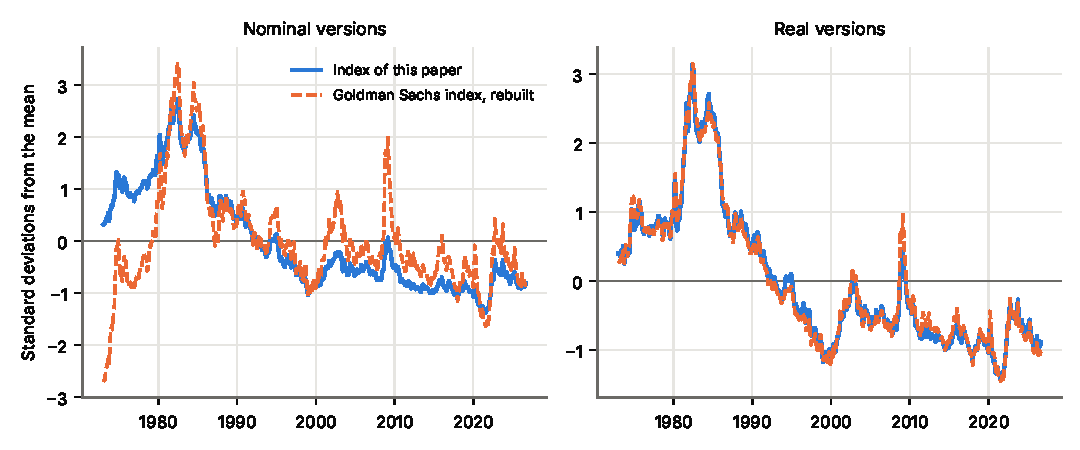
\includegraphics[width=\textwidth]{../baseline/report/fig_gs.pdf}
\caption{The Index and the Goldman Sachs Index, Nominal and Real Versions}
\label{fig:gs}
\begin{flushleft}\footnotesize\textit{Notes:} Monthly, January 1973 to September 2026, each series in units of its standard deviation from its mean. The Goldman Sachs index is rebuilt from public data with its published weights (companion paper), in the same version as the index of this paper. Left: nominal versions. Right: real versions, with the 10-year yield less 10-year expected inflation.\end{flushleft}
\end{figure}

\begin{figure}[tp]
\centering
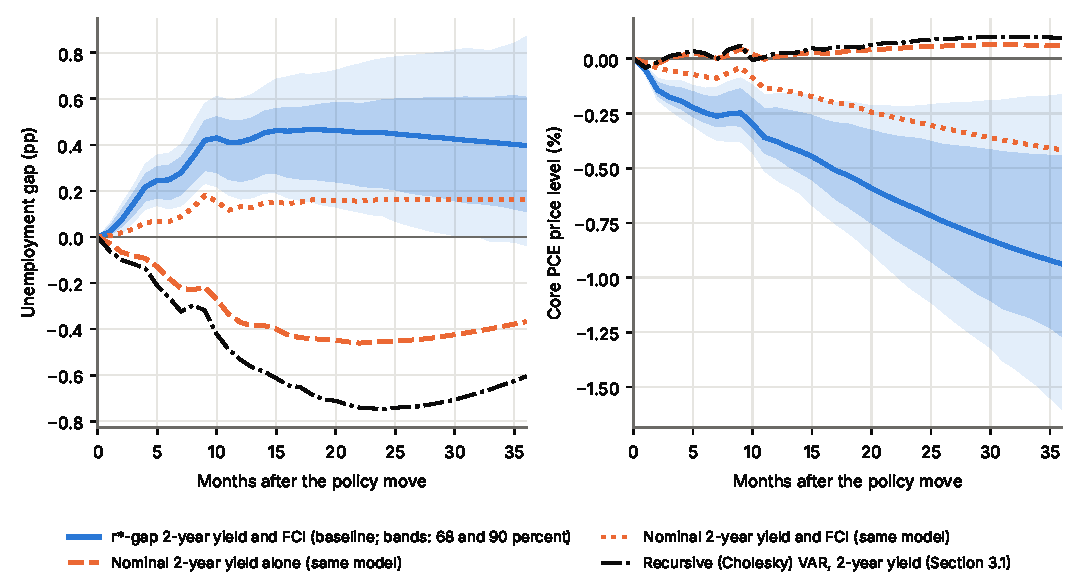
\includegraphics[width=\textwidth]{../baseline/report/fig_size.pdf}
\caption{Responses to a Policy Move: Baseline, Nominal Yield Alone and with the FCI, and Cholesky VAR}
\label{fig:size}
\begin{flushleft}\footnotesize\textit{Notes:} Policy move that raises the two-year yield 1 percentage point. Baseline: two-year yield and FCI relative to $\rs$; 12 lags; shaded bands 68 and 90 percent. The nominal yield alone and with the FCI are in the same model; the Cholesky VAR is that of Section~\ref{sec:standard}.\end{flushleft}
\end{figure}

\begin{table}[tp]\centering\footnotesize\setlength{\tabcolsep}{2.2pt}
\caption{Baselines: Monthly Equations from 1996 and from 1973, March-December 2020 Dropped (12 Lags)}\label{tab:mainB}
\resizebox{\ifdim\width>\textwidth\textwidth\else\width\fi}{!}{%
\begin{tabular}{llcrrrrrrr}\toprule
 & & & & \multicolumn{3}{c}{Unemployment gap (pp)} & \multicolumn{3}{c}{Price level (\%)}\\ \cmidrule(lr){5-7}\cmidrule(lr){8-10}
Case & FCI & Lags & Obs & 12 m & 24 m & 36 m & 12 m & 24 m & 36 m\\ \midrule
Baseline, 1996: Nominal & none & 12 & 359 & $-$0.37$^{**}$ & $-$0.45$^{**}$ & $-$0.37$^{*}$ & 0.01 & 0.06 & 0.06\\
 & & & & {\scriptsize [$-$0.55, $-$0.18]} & {\scriptsize [$-$0.69, $-$0.17]} & {\scriptsize [$-$0.64, $-$0.02]} & {\scriptsize [$-$0.13, 0.19]} & {\scriptsize [$-$0.21, 0.40]} & {\scriptsize [$-$0.33, 0.55]}\\
 & nominal & 12 & 359 & 0.13 & 0.16 & 0.16 & $-$0.14 & $-$0.29 & $-$0.42\\
 & & & & {\scriptsize [$-$0.04, 0.36]} & {\scriptsize [$-$0.08, 0.49]} & {\scriptsize [$-$0.12, 0.52]} & {\scriptsize [$-$0.33, 0.07]} & {\scriptsize [$-$0.69, 0.10]} & {\scriptsize [$-$1.02, 0.17]}\\
\addlinespace
Baseline, 1996: Real & none & 12 & 359 & $-$0.28$^{**}$ & $-$0.35$^{**}$ & $-$0.30$^{*}$ & $-$0.08 & $-$0.06 & $-$0.06\\
 & & & & {\scriptsize [$-$0.45, $-$0.11]} & {\scriptsize [$-$0.57, $-$0.11]} & {\scriptsize [$-$0.56, $-$0.03]} & {\scriptsize [$-$0.19, 0.08]} & {\scriptsize [$-$0.28, 0.21]} & {\scriptsize [$-$0.37, 0.33]}\\
 & real & 12 & 359 & 0.17$^{*}$ & 0.23$^{*}$ & 0.22 & $-$0.22$^{**}$ & $-$0.38$^{**}$ & $-$0.50$^{*}$\\
 & & & & {\scriptsize [0.01, 0.35]} & {\scriptsize [0.00, 0.50]} & {\scriptsize [$-$0.04, 0.57]} & {\scriptsize [$-$0.38, $-$0.05]} & {\scriptsize [$-$0.75, $-$0.07]} & {\scriptsize [$-$1.03, $-$0.05]}\\
\addlinespace
Baseline, 1996: r*-gap & none & 12 & 359 & $-$0.10 & $-$0.21 & $-$0.25 & $-$0.20$^{**}$ & $-$0.32 & $-$0.44\\
 & & & & {\scriptsize [$-$0.28, 0.10]} & {\scriptsize [$-$0.47, 0.08]} & {\scriptsize [$-$0.54, 0.11]} & {\scriptsize [$-$0.35, $-$0.03]} & {\scriptsize [$-$0.63, 0.03]} & {\scriptsize [$-$0.91, 0.06]}\\
 & r*-gap & 12 & 359 & 0.41$^{**}$ & 0.45$^{**}$ & 0.40 & $-$0.38$^{**}$ & $-$0.69$^{**}$ & $-$0.94$^{**}$\\
 & & & & {\scriptsize [0.16, 0.60]} & {\scriptsize [0.09, 0.78]} & {\scriptsize [$-$0.04, 0.87]} & {\scriptsize [$-$0.55, $-$0.16]} & {\scriptsize [$-$1.08, $-$0.21]} & {\scriptsize [$-$1.60, $-$0.16]}\\
\addlinespace
Baseline, 1973: Nominal & none & 12 & 623 & 0.11 & 0.17 & 0.13 & $-$0.01 & $-$0.08 & $-$0.15\\
 & & & & {\scriptsize [$-$0.03, 0.23]} & {\scriptsize [$-$0.01, 0.27]} & {\scriptsize [$-$0.04, 0.21]} & {\scriptsize [$-$0.12, 0.13]} & {\scriptsize [$-$0.27, 0.24]} & {\scriptsize [$-$0.42, 0.35]}\\
 & nominal & 12 & 623 & 0.29$^{**}$ & 0.19 & 0.06 & $-$0.01 & $-$0.17 & $-$0.33\\
 & & & & {\scriptsize [0.13, 0.41]} & {\scriptsize [$-$0.01, 0.30]} & {\scriptsize [$-$0.14, 0.20]} & {\scriptsize [$-$0.13, 0.12]} & {\scriptsize [$-$0.33, 0.10]} & {\scriptsize [$-$0.56, 0.08]}\\
\addlinespace
Baseline, 1973: Real & none & 12 & 623 & 0.09 & 0.08 & 0.02 & $-$0.23$^{**}$ & $-$0.49$^{**}$ & $-$0.72$^{**}$\\
 & & & & {\scriptsize [$-$0.02, 0.20]} & {\scriptsize [$-$0.07, 0.19]} & {\scriptsize [$-$0.13, 0.13]} & {\scriptsize [$-$0.31, $-$0.10]} & {\scriptsize [$-$0.64, $-$0.18]} & {\scriptsize [$-$0.97, $-$0.20]}\\
 & real & 12 & 623 & 0.25$^{**}$ & 0.13 & 0.02 & $-$0.24$^{**}$ & $-$0.55$^{**}$ & $-$0.79$^{**}$\\
 & & & & {\scriptsize [0.11, 0.35]} & {\scriptsize [$-$0.07, 0.26]} & {\scriptsize [$-$0.15, 0.17]} & {\scriptsize [$-$0.33, $-$0.11]} & {\scriptsize [$-$0.69, $-$0.25]} & {\scriptsize [$-$1.01, $-$0.31]}\\
\addlinespace
Baseline, 1973: r*-gap & none & 12 & 623 & 0.17$^{**}$ & 0.15 & 0.05 & $-$0.28$^{**}$ & $-$0.64$^{**}$ & $-$0.97$^{**}$\\
 & & & & {\scriptsize [0.04, 0.29]} & {\scriptsize [$-$0.03, 0.31]} & {\scriptsize [$-$0.14, 0.22]} & {\scriptsize [$-$0.37, $-$0.16]} & {\scriptsize [$-$0.83, $-$0.32]} & {\scriptsize [$-$1.27, $-$0.45]}\\
 & r*-gap & 12 & 623 & 0.33$^{**}$ & 0.24 & 0.15 & $-$0.32$^{**}$ & $-$0.76$^{**}$ & $-$1.14$^{**}$\\
 & & & & {\scriptsize [0.14, 0.46]} & {\scriptsize [$-$0.02, 0.40]} & {\scriptsize [$-$0.09, 0.35]} & {\scriptsize [$-$0.42, $-$0.16]} & {\scriptsize [$-$0.93, $-$0.36]} & {\scriptsize [$-$1.45, $-$0.50]}\\
\bottomrule\end{tabular}}
\begin{flushleft}\footnotesize\textit{Notes:} Nominal, real and r*-gap 2-year yield; the FCI is the index in the matching form in each case. March-December 2020 dropped from the monthly and daily equations (values still enter as lags). From 1973: monthly series in place of daily data before 1990. Per +1 pp on the 2-year yield. $^{**}$ and $^{*}$: significant at the 5 and 10 percent levels (the 95\% and 90\% bootstrap intervals exclude zero); 90\% intervals in brackets. Obs = monthly observations in the equations.\end{flushleft}
\end{table}

\FloatBarrier
\begin{table}[tp]\centering\footnotesize\setlength{\tabcolsep}{3pt}
\caption{Responses without and with the FCI after Two Years, 1996--2026, with Paired Differences}\label{tab:matcheddiff}
\resizebox{\ifdim\width>\textwidth\textwidth\else\width\fi}{!}{%
\begin{tabular}{lcccccc}\toprule
 & \multicolumn{3}{c}{Unemployment gap (pp)} & \multicolumn{3}{c}{Price level (\%)}\\ \cmidrule(lr){2-4}\cmidrule(lr){5-7}
Yield measure & Yield alone & Yield and FCI & Difference & Yield alone & Yield and FCI & Difference\\ \midrule
Nominal & $-$0.45$^{**}$ & 0.16 & 0.62$^{**}$ & 0.06 & $-$0.29 & $-$0.35$^{*}$\\
 & {\scriptsize [$-$0.69, $-$0.17]} & {\scriptsize [$-$0.08, 0.49]} & {\scriptsize [0.34, 0.90]} & {\scriptsize [$-$0.21, 0.40]} & {\scriptsize [$-$0.69, 0.10]} & {\scriptsize [$-$0.75, $-$0.05]}\\
\addlinespace
Real & $-$0.35$^{**}$ & 0.23$^{*}$ & 0.57$^{**}$ & $-$0.06 & $-$0.38$^{**}$ & $-$0.32$^{*}$\\
 & {\scriptsize [$-$0.57, $-$0.11]} & {\scriptsize [0.00, 0.50]} & {\scriptsize [0.33, 0.86]} & {\scriptsize [$-$0.28, 0.21]} & {\scriptsize [$-$0.75, $-$0.07]} & {\scriptsize [$-$0.66, $-$0.05]}\\
\addlinespace
Neutral rate ($r^*$-gap) & $-$0.21 & 0.45$^{**}$ & 0.66$^{**}$ & $-$0.32 & $-$0.69$^{**}$ & $-$0.37\\
 & {\scriptsize [$-$0.47, 0.08]} & {\scriptsize [0.09, 0.78]} & {\scriptsize [0.27, 1.00]} & {\scriptsize [$-$0.63, 0.03]} & {\scriptsize [$-$1.08, $-$0.21]} & {\scriptsize [$-$0.72, 0.03]}\\
\bottomrule\end{tabular}}
\begin{flushleft}\footnotesize\textit{Notes:} Responses 24 months after a policy move that raises the two-year yield 1 pp in the window, 1996--2026, 12 lags. Differences are computed on common bootstrap draws before rounding. Brackets: 90\% intervals; $^{**}$, $^{*}$: 5 and 10 percent levels. Responses at 12 and 36 months and at 3 and 6 lags are in Appendix Tables~\ref{tab:mainB} and~\ref{tab:lags}.\end{flushleft}
\end{table}

\begin{table}[tp]\centering\small
\caption{Implied Trade-Off: Phillips Multiplier $\kappa_H$ (12 Lags), All Cases}\label{tab:tradefull}
\resizebox{\ifdim\width>\textwidth\textwidth\else\width\fi}{!}{%
\begin{tabular}{llrr}\toprule Case & FCI & $H=24$ months & $H=36$ months\\ \midrule
\multicolumn{4}{l}{\textit{Baseline, 1996}}\\
Nominal & none & $-$0.09 [$-$0.62, 0.55] & $-$0.06 [$-$0.53, 0.55]\\
 & nominal & $-$1.21 (undefined; 68\%: [$-$3.29, $-$0.30]) & $-$1.03 (undefined; 68\%: [$-$2.96, $-$0.31])\\
Real & none & 0.14 [$-$0.44, 1.10] & 0.08 [$-$0.41, 1.00]\\
 & real & $-$1.16 [$-$5.51, $-$0.25] & $-$0.90 [$-$7.04, $-$0.07]\\
r*-gap & none & 1.94 (undefined; 68\%: undefined) & 1.07 (undefined; 68\%: undefined)\\
 & r*-gap & $-$0.95 [$-$1.99, $-$0.32] & $-$0.81 [$-$2.12, $-$0.18]\\
\addlinespace
\multicolumn{4}{l}{\textit{Baseline, 1973}}\\
Nominal & none & $-$0.44 (undefined; 68\%: [$-$1.75, 1.96]) & $-$0.46 (undefined; 68\%: [$-$1.29, 1.41])\\
 & nominal & $-$0.41 [$-$0.96, 0.38] & $-$0.62 [$-$1.67, 0.36]\\
Real & none & $-$3.78 (undefined; 68\%: [$-$35.33, $-$1.85]) & $-$4.02 (undefined; 68\%: undefined)\\
 & real & $-$1.56 [$-$3.72, $-$0.75] & $-$1.89 [$-$18.61, $-$0.79]\\
r*-gap & none & $-$2.37 [$-$12.49, $-$1.08] & $-$2.68 (undefined; 68\%: [$-$6.29, $-$1.52])\\
 & r*-gap & $-$1.49 [$-$2.92, $-$0.72] & $-$1.64 [$-$5.39, $-$0.72]\\
\addlinespace
\multicolumn{4}{l}{\textit{Variations, $r^*$-gap with the FCI}}\\
2020 left in, 1996 & r*-gap & $-$1.07 [$-$3.87, $-$0.51] & $-$0.91 [$-$3.65, $-$0.39]\\
2020 left in, 1973 & r*-gap & $-$2.24 (undefined; 68\%: [$-$32.30, $-$1.26]) & $-$2.37 (undefined; 68\%: undefined)\\
Ends 2019, 1996 & r*-gap & $-$0.31 (undefined; 68\%: [$-$1.03, 0.01]) & $-$0.42 (undefined; 68\%: undefined)\\
Ends 2019, 1973 & r*-gap & $-$1.21 [$-$6.48, $-$0.39] & $-$1.58 (undefined; 68\%: [$-$8.00, $-$0.86])\\
Kiley r*, 1996 & r*-gap (Kiley) & $-$0.13 (undefined; 68\%: undefined) & 1.35 (undefined; 68\%: undefined)\\
Kiley r*, 1973 & r*-gap (Kiley) & $-$2.81 (undefined; 68\%: [$-$7.40, $-$1.60]) & $-$3.80 (undefined; 68\%: [$-$241.63, $-$1.77])\\
Real, spline trend, 1996 & real & $-$0.86 (undefined; 68\%: [$-$8.09, $-$0.07]) & $-$0.73 (undefined; 68\%: undefined)\\
Real, spline trend, 1973 & real & $-$0.97 [$-$1.95, $-$0.53] & $-$0.85 [$-$2.03, $-$0.45]\\
\addlinespace
r*-gap minus nominal, with FCI & & [$-$1.74, 2.36] & [$-$1.46, 2.26]\\
\bottomrule\end{tabular}}
\begin{flushleft}\footnotesize\textit{Notes:} $\kappa_H$ = core PCE price level at month $H$ (percent) per percentage-point year of cumulative unemployment-gap response (Barnichon and Mesters 2021); the sacrifice ratio is $-1/\kappa_H$. Point estimate and 90\% confidence set (Anderson--Rubin type) in brackets, computed exactly (a wide grid refined by bisection), so a finite end is never an artifact of the grid. An infinite end means that the 90\% interval of the cumulative unemployment response includes zero: the data then cannot rule out arbitrarily steep trade-offs on that side; ``unbounded'': both sides. Last row: paired difference over common announcement draws.\end{flushleft}
\end{table}

\FloatBarrier
\begin{table}[tp]\centering\footnotesize\setlength{\tabcolsep}{2.2pt}
\caption{Sample (r*-gap 2-Year Yield and FCI) (12 Lags)}\label{tab:mainR1}
\resizebox{\ifdim\width>\textwidth\textwidth\else\width\fi}{!}{%
\begin{tabular}{llcrrrrrrr}\toprule
 & & & & \multicolumn{3}{c}{Unemployment gap (pp)} & \multicolumn{3}{c}{Price level (\%)}\\ \cmidrule(lr){5-7}\cmidrule(lr){8-10}
Case & FCI & Lags & Obs & 12 m & 24 m & 36 m & 12 m & 24 m & 36 m\\ \midrule
Start 1973 & none & 12 & 633 & $-$0.05 & $-$0.01 & 0.00 & $-$0.22$^{**}$ & $-$0.50$^{**}$ & $-$0.79$^{**}$\\
 & & & & {\scriptsize [$-$0.20, 0.08]} & {\scriptsize [$-$0.17, 0.16]} & {\scriptsize [$-$0.16, 0.17]} & {\scriptsize [$-$0.33, $-$0.08]} & {\scriptsize [$-$0.73, $-$0.17]} & {\scriptsize [$-$1.17, $-$0.21]}\\
 & r*-gap & 12 & 633 & 0.18 & 0.14 & 0.13 & $-$0.27$^{**}$ & $-$0.63$^{**}$ & $-$0.98$^{**}$\\
 & & & & {\scriptsize [$-$0.07, 0.38]} & {\scriptsize [$-$0.17, 0.36]} & {\scriptsize [$-$0.19, 0.35]} & {\scriptsize [$-$0.41, $-$0.10]} & {\scriptsize [$-$0.89, $-$0.22]} & {\scriptsize [$-$1.42, $-$0.26]}\\
\addlinespace
2020 dropped & none & 12 & 359 & $-$0.10 & $-$0.21 & $-$0.25 & $-$0.20$^{**}$ & $-$0.32 & $-$0.44\\
 & & & & {\scriptsize [$-$0.28, 0.10]} & {\scriptsize [$-$0.47, 0.08]} & {\scriptsize [$-$0.54, 0.11]} & {\scriptsize [$-$0.35, $-$0.03]} & {\scriptsize [$-$0.63, 0.03]} & {\scriptsize [$-$0.91, 0.06]}\\
 & r*-gap & 12 & 359 & 0.41$^{**}$ & 0.45$^{**}$ & 0.40 & $-$0.38$^{**}$ & $-$0.69$^{**}$ & $-$0.94$^{**}$\\
 & & & & {\scriptsize [0.16, 0.60]} & {\scriptsize [0.09, 0.78]} & {\scriptsize [$-$0.04, 0.87]} & {\scriptsize [$-$0.55, $-$0.16]} & {\scriptsize [$-$1.08, $-$0.21]} & {\scriptsize [$-$1.60, $-$0.16]}\\
\addlinespace
2020 dropped, start 1973 & none & 12 & 623 & 0.17$^{**}$ & 0.15 & 0.05 & $-$0.28$^{**}$ & $-$0.64$^{**}$ & $-$0.97$^{**}$\\
 & & & & {\scriptsize [0.04, 0.29]} & {\scriptsize [$-$0.03, 0.31]} & {\scriptsize [$-$0.14, 0.22]} & {\scriptsize [$-$0.37, $-$0.16]} & {\scriptsize [$-$0.83, $-$0.32]} & {\scriptsize [$-$1.27, $-$0.45]}\\
 & r*-gap & 12 & 623 & 0.33$^{**}$ & 0.24 & 0.15 & $-$0.32$^{**}$ & $-$0.76$^{**}$ & $-$1.14$^{**}$\\
 & & & & {\scriptsize [0.14, 0.46]} & {\scriptsize [$-$0.02, 0.40]} & {\scriptsize [$-$0.09, 0.35]} & {\scriptsize [$-$0.42, $-$0.16]} & {\scriptsize [$-$0.93, $-$0.36]} & {\scriptsize [$-$1.45, $-$0.50]}\\
\addlinespace
Ends 2019 & none & 12 & 288 & $-$0.15 & $-$0.24 & $-$0.26 & 0.08 & 0.06 & 0.03\\
 & & & & {\scriptsize [$-$0.37, 0.11]} & {\scriptsize [$-$0.62, 0.19]} & {\scriptsize [$-$0.75, 0.26]} & {\scriptsize [$-$0.05, 0.20]} & {\scriptsize [$-$0.10, 0.20]} & {\scriptsize [$-$0.17, 0.22]}\\
 & r*-gap & 12 & 288 & 0.30$^{*}$ & 0.14 & 0.00 & $-$0.08 & $-$0.14 & $-$0.21\\
 & & & & {\scriptsize [0.04, 0.55]} & {\scriptsize [$-$0.30, 0.49]} & {\scriptsize [$-$0.47, 0.43]} & {\scriptsize [$-$0.23, 0.08]} & {\scriptsize [$-$0.38, 0.09]} & {\scriptsize [$-$0.53, 0.09]}\\
\addlinespace
Ends 2019, start 1973 & none & 12 & 552 & 0.19$^{**}$ & 0.18 & 0.08 & $-$0.21$^{**}$ & $-$0.49$^{**}$ & $-$0.82$^{**}$\\
 & & & & {\scriptsize [0.06, 0.31]} & {\scriptsize [$-$0.04, 0.32]} & {\scriptsize [$-$0.17, 0.25]} & {\scriptsize [$-$0.31, $-$0.06]} & {\scriptsize [$-$0.69, $-$0.15]} & {\scriptsize [$-$1.20, $-$0.25]}\\
 & r*-gap & 12 & 552 & 0.27$^{**}$ & 0.16 & 0.10 & $-$0.22$^{**}$ & $-$0.50$^{**}$ & $-$0.84$^{**}$\\
 & & & & {\scriptsize [0.06, 0.41]} & {\scriptsize [$-$0.16, 0.35]} & {\scriptsize [$-$0.23, 0.28]} & {\scriptsize [$-$0.33, $-$0.06]} & {\scriptsize [$-$0.70, $-$0.16]} & {\scriptsize [$-$1.19, $-$0.23]}\\
\bottomrule\end{tabular}}
\begin{flushleft}\footnotesize\textit{Notes:} Start 1973: monthly equations from 1973, with monthly series in place of daily data before 1990. 2020 dropped: March to December 2020 removed from the monthly and daily equations (2020 values still enter as lags). Ends 2019: all equations, monthly and daily. Per +1 pp on the 2-year yield. $^{**}$ and $^{*}$: significant at the 5 and 10 percent levels (the 95\% and 90\% bootstrap intervals exclude zero); 90\% intervals in brackets. Obs = monthly observations in the equations.\end{flushleft}
\end{table}

\FloatBarrier
\begin{table}[tp]\centering\footnotesize\setlength{\tabcolsep}{2.2pt}
\caption{the r* Adjustment and Trends (12 Lags)}\label{tab:mainR2}
\resizebox{\ifdim\width>\textwidth\textwidth\else\width\fi}{!}{%
\begin{tabular}{llcrrrrrrr}\toprule
 & & & & \multicolumn{3}{c}{Unemployment gap (pp)} & \multicolumn{3}{c}{Price level (\%)}\\ \cmidrule(lr){5-7}\cmidrule(lr){8-10}
Case & FCI & Lags & Obs & 12 m & 24 m & 36 m & 12 m & 24 m & 36 m\\ \midrule
Kiley r*, 1996 & none & 12 & 359 & $-$0.25$^{**}$ & $-$0.37$^{**}$ & $-$0.36$^{**}$ & $-$0.12 & $-$0.10 & $-$0.07\\
 & & & & {\scriptsize [$-$0.41, $-$0.09]} & {\scriptsize [$-$0.58, $-$0.12]} & {\scriptsize [$-$0.59, $-$0.06]} & {\scriptsize [$-$0.24, 0.03]} & {\scriptsize [$-$0.34, 0.20]} & {\scriptsize [$-$0.45, 0.35]}\\
 & r*-gap (Kiley) & 12 & 359 & 0.10 & $-$0.02 & $-$0.08 & $-$0.14 & $-$0.02 & 0.12\\
 & & & & {\scriptsize [$-$0.08, 0.30]} & {\scriptsize [$-$0.31, 0.31]} & {\scriptsize [$-$0.34, 0.26]} & {\scriptsize [$-$0.31, 0.01]} & {\scriptsize [$-$0.40, 0.27]} & {\scriptsize [$-$0.48, 0.52]}\\
\addlinespace
Kiley r*, 1973 & none & 12 & 623 & 0.11 & 0.07 & 0.00 & $-$0.25$^{**}$ & $-$0.51$^{**}$ & $-$0.72$^{**}$\\
 & & & & {\scriptsize [$-$0.02, 0.21]} & {\scriptsize [$-$0.09, 0.18]} & {\scriptsize [$-$0.17, 0.12]} & {\scriptsize [$-$0.34, $-$0.14]} & {\scriptsize [$-$0.68, $-$0.26]} & {\scriptsize [$-$1.00, $-$0.33]}\\
 & r*-gap (Kiley) & 12 & 623 & 0.14 & 0.02 & 0.00 & $-$0.26$^{**}$ & $-$0.52$^{**}$ & $-$0.72$^{**}$\\
 & & & & {\scriptsize [0.00, 0.24]} & {\scriptsize [$-$0.12, 0.16]} & {\scriptsize [$-$0.12, 0.13]} & {\scriptsize [$-$0.35, $-$0.15]} & {\scriptsize [$-$0.68, $-$0.26]} & {\scriptsize [$-$0.95, $-$0.29]}\\
\addlinespace
Real, spline trend, 1996 & none & 12 & 359 & $-$0.29$^{**}$ & $-$0.29$^{**}$ & $-$0.17 & $-$0.05 & $-$0.09 & $-$0.21\\
 & & & & {\scriptsize [$-$0.48, $-$0.17]} & {\scriptsize [$-$0.54, $-$0.07]} & {\scriptsize [$-$0.46, 0.05]} & {\scriptsize [$-$0.16, 0.14]} & {\scriptsize [$-$0.33, 0.22]} & {\scriptsize [$-$0.58, 0.21]}\\
 & real & 12 & 359 & 0.18 & 0.20 & 0.18 & $-$0.15 & $-$0.29 & $-$0.39\\
 & & & & {\scriptsize [$-$0.05, 0.31]} & {\scriptsize [$-$0.17, 0.43]} & {\scriptsize [$-$0.19, 0.41]} & {\scriptsize [$-$0.31, 0.07]} & {\scriptsize [$-$0.66, 0.15]} & {\scriptsize [$-$0.91, 0.27]}\\
\addlinespace
Real, spline trend, 1973 & none & 12 & 623 & 0.13$^{*}$ & 0.23$^{**}$ & 0.22$^{*}$ & $-$0.16$^{**}$ & $-$0.35$^{**}$ & $-$0.51$^{**}$\\
 & & & & {\scriptsize [0.00, 0.22]} & {\scriptsize [0.05, 0.36]} & {\scriptsize [0.02, 0.34]} & {\scriptsize [$-$0.23, $-$0.06]} & {\scriptsize [$-$0.53, $-$0.16]} & {\scriptsize [$-$0.77, $-$0.22]}\\
 & real & 12 & 623 & 0.29$^{**}$ & 0.28$^{**}$ & 0.19 & $-$0.21$^{**}$ & $-$0.46$^{**}$ & $-$0.60$^{**}$\\
 & & & & {\scriptsize [0.13, 0.41]} & {\scriptsize [0.04, 0.47]} & {\scriptsize [$-$0.03, 0.38]} & {\scriptsize [$-$0.30, $-$0.08]} & {\scriptsize [$-$0.66, $-$0.22]} & {\scriptsize [$-$0.91, $-$0.25]}\\
\bottomrule\end{tabular}}
\begin{flushleft}\footnotesize\textit{Notes:} Kiley r*: 2-year minus expected inflation minus Kiley's r*, with the index built with the same r*. Real, spline trend: real 2-year and real FCI with a natural cubic spline trend (knots at the sample ends and at NBER business-cycle peaks inside the sample) in every monthly equation, in place of any r* measure. Per +1 pp on the 2-year yield. $^{**}$ and $^{*}$: significant at the 5 and 10 percent levels (the 95\% and 90\% bootstrap intervals exclude zero); 90\% intervals in brackets. Obs = monthly observations in the equations.\end{flushleft}
\end{table}

\FloatBarrier
\begin{table}[tp]\centering\footnotesize\setlength{\tabcolsep}{2.2pt}
\caption{Credit (r*-gap) (12 Lags)}\label{tab:mainR3}
\resizebox{\ifdim\width>\textwidth\textwidth\else\width\fi}{!}{%
\begin{tabular}{llcrrrrrrr}\toprule
 & & & & \multicolumn{3}{c}{Unemployment gap (pp)} & \multicolumn{3}{c}{Price level (\%)}\\ \cmidrule(lr){5-7}\cmidrule(lr){8-10}
Case & FCI & Lags & Obs & 12 m & 24 m & 36 m & 12 m & 24 m & 36 m\\ \midrule
EBP added, 1996 & none & 12 & 359 & 0.10 & 0.06 & 0.08 & $-$0.20$^{**}$ & $-$0.34$^{*}$ & $-$0.49$^{*}$\\
 & & & & {\scriptsize [$-$0.07, 0.24]} & {\scriptsize [$-$0.25, 0.34]} & {\scriptsize [$-$0.30, 0.36]} & {\scriptsize [$-$0.33, $-$0.05]} & {\scriptsize [$-$0.62, $-$0.03]} & {\scriptsize [$-$0.90, $-$0.01]}\\
 & r*-gap & 12 & 359 & 0.39$^{**}$ & 0.44$^{*}$ & 0.34 & $-$0.33$^{**}$ & $-$0.59$^{**}$ & $-$0.82$^{*}$\\
 & & & & {\scriptsize [0.17, 0.54]} & {\scriptsize [0.02, 0.73]} & {\scriptsize [$-$0.20, 0.70]} & {\scriptsize [$-$0.47, $-$0.12]} & {\scriptsize [$-$0.92, $-$0.14]} & {\scriptsize [$-$1.34, $-$0.08]}\\
\addlinespace
EBP added, 1973 & none & 12 & 623 & 0.13$^{**}$ & 0.08 & 0.02 & $-$0.27$^{**}$ & $-$0.61$^{**}$ & $-$0.92$^{**}$\\
 & & & & {\scriptsize [0.02, 0.22]} & {\scriptsize [$-$0.08, 0.20]} & {\scriptsize [$-$0.14, 0.15]} & {\scriptsize [$-$0.36, $-$0.14]} & {\scriptsize [$-$0.80, $-$0.31]} & {\scriptsize [$-$1.26, $-$0.43]}\\
 & r*-gap & 12 & 623 & 0.22$^{**}$ & 0.14 & 0.09 & $-$0.31$^{**}$ & $-$0.71$^{**}$ & $-$1.07$^{**}$\\
 & & & & {\scriptsize [0.08, 0.33]} & {\scriptsize [$-$0.06, 0.28]} & {\scriptsize [$-$0.11, 0.24]} & {\scriptsize [$-$0.41, $-$0.15]} & {\scriptsize [$-$0.91, $-$0.34]} & {\scriptsize [$-$1.43, $-$0.45]}\\
\addlinespace
Baa spread in the daily block, 1996 & none & 12 & 359 & $-$0.10 & $-$0.21 & $-$0.25 & $-$0.20$^{**}$ & $-$0.32 & $-$0.44\\
 & & & & {\scriptsize [$-$0.28, 0.10]} & {\scriptsize [$-$0.47, 0.08]} & {\scriptsize [$-$0.54, 0.11]} & {\scriptsize [$-$0.35, $-$0.03]} & {\scriptsize [$-$0.63, 0.03]} & {\scriptsize [$-$0.91, 0.06]}\\
 & r*-gap + Baa spread & 12 & 359 & 0.31$^{*}$ & 0.34 & 0.25 & $-$0.32$^{**}$ & $-$0.60$^{*}$ & $-$0.84$^{*}$\\
 & & & & {\scriptsize [0.04, 0.52]} & {\scriptsize [$-$0.03, 0.74]} & {\scriptsize [$-$0.19, 0.78]} & {\scriptsize [$-$0.50, $-$0.06]} & {\scriptsize [$-$1.02, $-$0.09]} & {\scriptsize [$-$1.61, $-$0.09]}\\
\addlinespace
Baa spread in the daily block, 1973 & none & 12 & 623 & 0.17$^{**}$ & 0.15 & 0.05 & $-$0.28$^{**}$ & $-$0.64$^{**}$ & $-$0.97$^{**}$\\
 & & & & {\scriptsize [0.04, 0.29]} & {\scriptsize [$-$0.03, 0.31]} & {\scriptsize [$-$0.14, 0.22]} & {\scriptsize [$-$0.37, $-$0.16]} & {\scriptsize [$-$0.83, $-$0.32]} & {\scriptsize [$-$1.27, $-$0.45]}\\
 & r*-gap + Baa spread & 12 & 467 & 0.26 & 0.24 & 0.14 & $-$0.21 & $-$0.33 & $-$0.39\\
 & & & & {\scriptsize [$-$0.01, 0.45]} & {\scriptsize [$-$0.13, 0.52]} & {\scriptsize [$-$0.30, 0.44]} & {\scriptsize [$-$0.34, 0.05]} & {\scriptsize [$-$0.56, 0.25]} & {\scriptsize [$-$0.70, 0.53]}\\
\bottomrule\end{tabular}}
\begin{flushleft}\footnotesize\textit{Notes:} EBP added: the excess bond premium is a third monthly variable, treated like unemployment and inflation; responses shown for u and the price level. Baa spread: the daily Baa-10-year spread enters the daily block next to the yield and the FCI, with its announcement-day response as impact. Per +1 pp on the 2-year yield. $^{**}$ and $^{*}$: significant at the 5 and 10 percent levels (the 95\% and 90\% bootstrap intervals exclude zero); 90\% intervals in brackets. Obs = monthly observations in the equations.\end{flushleft}
\end{table}

\FloatBarrier
\begin{table}[tp]\centering\footnotesize\setlength{\tabcolsep}{2.2pt}
\caption{the FCI Replaced by Its Three Weighted Components (12 Lags)}\label{tab:mainR4}
\resizebox{\ifdim\width>\textwidth\textwidth\else\width\fi}{!}{%
\begin{tabular}{llcrrrrrrr}\toprule
 & & & & \multicolumn{3}{c}{Unemployment gap (pp)} & \multicolumn{3}{c}{Price level (\%)}\\ \cmidrule(lr){5-7}\cmidrule(lr){8-10}
Case & FCI & Lags & Obs & 12 m & 24 m & 36 m & 12 m & 24 m & 36 m\\ \midrule
Components, 1996: Nominal & components & 12 & 359 & 0.11 & 0.17 & 0.17 & $-$0.05 & 0.10 & 0.23\\
 & & & & {\scriptsize [$-$0.16, 0.36]} & {\scriptsize [$-$0.22, 0.63]} & {\scriptsize [$-$0.33, 0.72]} & {\scriptsize [$-$0.23, 0.21]} & {\scriptsize [$-$0.29, 0.58]} & {\scriptsize [$-$0.37, 0.90]}\\
\addlinespace
Components, 1996: Real & components & 12 & 359 & 0.08 & 0.12 & 0.10 & $-$0.09 & 0.05 & 0.17\\
 & & & & {\scriptsize [$-$0.12, 0.27]} & {\scriptsize [$-$0.18, 0.49]} & {\scriptsize [$-$0.22, 0.62]} & {\scriptsize [$-$0.25, 0.10]} & {\scriptsize [$-$0.30, 0.39]} & {\scriptsize [$-$0.34, 0.64]}\\
\addlinespace
Components, 1996: r*-gap & components & 12 & 359 & 0.29$^{*}$ & 0.33 & 0.23 & $-$0.18 & $-$0.07 & 0.08\\
 & & & & {\scriptsize [0.01, 0.44]} & {\scriptsize [$-$0.04, 0.59]} & {\scriptsize [$-$0.25, 0.58]} & {\scriptsize [$-$0.31, 0.04]} & {\scriptsize [$-$0.40, 0.40]} & {\scriptsize [$-$0.48, 0.78]}\\
\addlinespace
Components, 1973: Nominal & components & 12 & 623 & $-$0.01 & $-$0.23 & $-$0.37 & 0.01 & 0.26 & 0.68$^{*}$\\
 & & & & {\scriptsize [$-$0.30, 0.19]} & {\scriptsize [$-$0.65, 0.10]} & {\scriptsize [$-$0.79, 0.04]} & {\scriptsize [$-$0.18, 0.26]} & {\scriptsize [$-$0.11, 0.88]} & {\scriptsize [0.01, 1.73]}\\
\addlinespace
Components, 1973: Real & components & 12 & 623 & 0.00 & $-$0.23$^{*}$ & $-$0.32$^{**}$ & $-$0.17 & $-$0.10 & 0.14\\
 & & & & {\scriptsize [$-$0.29, 0.14]} & {\scriptsize [$-$0.64, $-$0.05]} & {\scriptsize [$-$0.75, $-$0.07]} & {\scriptsize [$-$0.33, 0.10]} & {\scriptsize [$-$0.37, 0.57]} & {\scriptsize [$-$0.37, 1.30]}\\
\addlinespace
Components, 1973: r*-gap & components & 12 & 623 & 0.24 & 0.08 & $-$0.06 & $-$0.35$^{**}$ & $-$0.57 & $-$0.70\\
 & & & & {\scriptsize [$-$0.02, 0.44]} & {\scriptsize [$-$0.31, 0.39]} & {\scriptsize [$-$0.46, 0.25]} & {\scriptsize [$-$0.53, $-$0.13]} & {\scriptsize [$-$0.90, 0.04]} & {\scriptsize [$-$1.16, 0.37]}\\
\bottomrule\end{tabular}}
\begin{flushleft}\footnotesize\textit{Notes:} Components: the 10-year yield, equity valuation and real dollar, each multiplied by its weight, enter separately in the daily and monthly equations in the same version as the 2-year yield, each with its own window impact (the three impacts sum to the FCI's). Per +1 pp on the 2-year yield. $^{**}$ and $^{*}$: significant at the 5 and 10 percent levels (the 95\% and 90\% bootstrap intervals exclude zero); 90\% intervals in brackets. Obs = monthly observations in the equations.\end{flushleft}
\end{table}

\FloatBarrier
\begin{table}[tp]\centering\footnotesize\setlength{\tabcolsep}{2.2pt}
\caption{Alternative Surprises (r*-gap) (12 Lags)}\label{tab:mainR5}
\resizebox{\ifdim\width>\textwidth\textwidth\else\width\fi}{!}{%
\begin{tabular}{llcrrrrrrr}\toprule
 & & & & \multicolumn{3}{c}{Unemployment gap (pp)} & \multicolumn{3}{c}{Price level (\%)}\\ \cmidrule(lr){5-7}\cmidrule(lr){8-10}
Case & FCI & Lags & Obs & 12 m & 24 m & 36 m & 12 m & 24 m & 36 m\\ \midrule
Bauer-Swanson surprise, 1996 & none & 12 & 359 & $-$0.10 & $-$0.21 & $-$0.25 & $-$0.20$^{**}$ & $-$0.32 & $-$0.44\\
 & & & & {\scriptsize [$-$0.28, 0.10]} & {\scriptsize [$-$0.47, 0.08]} & {\scriptsize [$-$0.54, 0.11]} & {\scriptsize [$-$0.35, $-$0.03]} & {\scriptsize [$-$0.63, 0.03]} & {\scriptsize [$-$0.91, 0.06]}\\
 & r*-gap & 12 & 359 & 0.46$^{**}$ & 0.49$^{**}$ & 0.43 & $-$0.39$^{**}$ & $-$0.72$^{**}$ & $-$0.98$^{**}$\\
 & & & & {\scriptsize [0.19, 0.67]} & {\scriptsize [0.11, 0.85]} & {\scriptsize [$-$0.02, 0.95]} & {\scriptsize [$-$0.57, $-$0.16]} & {\scriptsize [$-$1.14, $-$0.22]} & {\scriptsize [$-$1.69, $-$0.17]}\\
\addlinespace
Bauer-Swanson surprise, 1973 & none & 12 & 623 & 0.18$^{**}$ & 0.15 & 0.05 & $-$0.28$^{**}$ & $-$0.64$^{**}$ & $-$0.97$^{**}$\\
 & & & & {\scriptsize [0.04, 0.29]} & {\scriptsize [$-$0.03, 0.31]} & {\scriptsize [$-$0.14, 0.22]} & {\scriptsize [$-$0.37, $-$0.16]} & {\scriptsize [$-$0.83, $-$0.32]} & {\scriptsize [$-$1.27, $-$0.45]}\\
 & r*-gap & 12 & 623 & 0.36$^{**}$ & 0.27$^{*}$ & 0.16 & $-$0.33$^{**}$ & $-$0.78$^{**}$ & $-$1.17$^{**}$\\
 & & & & {\scriptsize [0.16, 0.50]} & {\scriptsize [0.01, 0.44]} & {\scriptsize [$-$0.09, 0.36]} & {\scriptsize [$-$0.43, $-$0.15]} & {\scriptsize [$-$0.96, $-$0.37]} & {\scriptsize [$-$1.50, $-$0.50]}\\
\addlinespace
Jarocinski-Karadi surprise, 1996 & none & 12 & 359 & $-$0.10 & $-$0.21 & $-$0.25 & $-$0.20$^{**}$ & $-$0.32 & $-$0.44\\
 & & & & {\scriptsize [$-$0.28, 0.11]} & {\scriptsize [$-$0.47, 0.08]} & {\scriptsize [$-$0.53, 0.11]} & {\scriptsize [$-$0.35, $-$0.03]} & {\scriptsize [$-$0.63, 0.03]} & {\scriptsize [$-$0.91, 0.06]}\\
 & r*-gap & 12 & 359 & 0.47$^{**}$ & 0.51$^{**}$ & 0.44 & $-$0.40$^{**}$ & $-$0.73$^{**}$ & $-$0.99$^{**}$\\
 & & & & {\scriptsize [0.21, 0.68]} & {\scriptsize [0.12, 0.86]} & {\scriptsize [$-$0.01, 0.95]} & {\scriptsize [$-$0.59, $-$0.17]} & {\scriptsize [$-$1.14, $-$0.23]} & {\scriptsize [$-$1.69, $-$0.17]}\\
\addlinespace
Jarocinski-Karadi surprise, 1973 & none & 12 & 623 & 0.17$^{**}$ & 0.15 & 0.05 & $-$0.28$^{**}$ & $-$0.64$^{**}$ & $-$0.97$^{**}$\\
 & & & & {\scriptsize [0.04, 0.29]} & {\scriptsize [$-$0.03, 0.31]} & {\scriptsize [$-$0.14, 0.22]} & {\scriptsize [$-$0.37, $-$0.16]} & {\scriptsize [$-$0.83, $-$0.32]} & {\scriptsize [$-$1.27, $-$0.45]}\\
 & r*-gap & 12 & 623 & 0.38$^{**}$ & 0.27$^{*}$ & 0.17 & $-$0.33$^{**}$ & $-$0.78$^{**}$ & $-$1.17$^{**}$\\
 & & & & {\scriptsize [0.17, 0.51]} & {\scriptsize [0.02, 0.45]} & {\scriptsize [$-$0.09, 0.37]} & {\scriptsize [$-$0.43, $-$0.15]} & {\scriptsize [$-$0.96, $-$0.36]} & {\scriptsize [$-$1.49, $-$0.49]}\\
\bottomrule\end{tabular}}
\begin{flushleft}\footnotesize\textit{Notes:} Bauer-Swanson: orthogonalized surprise of Bauer and Swanson (2023), announcements through 2019. Jarocinski-Karadi: Nakamura-Steinsson surprise kept when the 2-year yield and the S\&P 500 move in opposite directions in the window. The window impact and the bootstrap use the events with a surprise. Per +1 pp on the 2-year yield. $^{**}$ and $^{*}$: significant at the 5 and 10 percent levels (the 95\% and 90\% bootstrap intervals exclude zero); 90\% intervals in brackets. Obs = monthly observations in the equations.\end{flushleft}
\end{table}

\FloatBarrier
\begin{table}[tp]\centering\footnotesize\setlength{\tabcolsep}{2.2pt}
\caption{Other Calibrations of the Index Weights (r*-gap) (12 Lags)}\label{tab:mainR6}
\resizebox{\ifdim\width>\textwidth\textwidth\else\width\fi}{!}{%
\begin{tabular}{llcrrrrrrr}\toprule
 & & & & \multicolumn{3}{c}{Unemployment gap (pp)} & \multicolumn{3}{c}{Price level (\%)}\\ \cmidrule(lr){5-7}\cmidrule(lr){8-10}
Case & FCI & Lags & Obs & 12 m & 24 m & 36 m & 12 m & 24 m & 36 m\\ \midrule
Other weight calibrations, 1996 & r*-gap (Y weights) & 12 & 359 & 0.23$^{*}$ & 0.18 & 0.10 & $-$0.26$^{**}$ & $-$0.44$^{*}$ & $-$0.58\\
 & & & & {\scriptsize [0.02, 0.40]} & {\scriptsize [$-$0.12, 0.46]} & {\scriptsize [$-$0.28, 0.48]} & {\scriptsize [$-$0.40, $-$0.07]} & {\scriptsize [$-$0.76, $-$0.05]} & {\scriptsize [$-$1.13, 0.05]}\\
 & r*-gap (FRB/US weights) & 12 & 359 & 0.23$^{*}$ & 0.09 & $-$0.09 & $-$0.28$^{**}$ & $-$0.39 & $-$0.42\\
 & & & & {\scriptsize [0.02, 0.43]} & {\scriptsize [$-$0.27, 0.44]} & {\scriptsize [$-$0.50, 0.37]} & {\scriptsize [$-$0.46, $-$0.07]} & {\scriptsize [$-$0.76, 0.05]} & {\scriptsize [$-$1.04, 0.27]}\\
 & r*-gap (GS weights) & 12 & 359 & 0.42$^{**}$ & 0.46$^{**}$ & 0.40 & $-$0.40$^{**}$ & $-$0.72$^{**}$ & $-$0.98$^{**}$\\
 & & & & {\scriptsize [0.17, 0.61]} & {\scriptsize [0.09, 0.79]} & {\scriptsize [$-$0.04, 0.89]} & {\scriptsize [$-$0.57, $-$0.17]} & {\scriptsize [$-$1.12, $-$0.24]} & {\scriptsize [$-$1.69, $-$0.18]}\\
\addlinespace
Other weight calibrations, 1973 & r*-gap (Y weights) & 12 & 623 & 0.21$^{**}$ & 0.11 & 0.05 & $-$0.32$^{**}$ & $-$0.69$^{**}$ & $-$1.03$^{**}$\\
 & & & & {\scriptsize [0.06, 0.33]} & {\scriptsize [$-$0.10, 0.27]} & {\scriptsize [$-$0.14, 0.23]} & {\scriptsize [$-$0.40, $-$0.18]} & {\scriptsize [$-$0.88, $-$0.36]} & {\scriptsize [$-$1.34, $-$0.48]}\\
 & r*-gap (FRB/US weights) & 12 & 623 & 0.34$^{**}$ & 0.16 & 0.02 & $-$0.34$^{**}$ & $-$0.75$^{**}$ & $-$1.09$^{**}$\\
 & & & & {\scriptsize [0.16, 0.48]} & {\scriptsize [$-$0.07, 0.36]} & {\scriptsize [$-$0.17, 0.22]} & {\scriptsize [$-$0.45, $-$0.17]} & {\scriptsize [$-$0.94, $-$0.37]} & {\scriptsize [$-$1.46, $-$0.46]}\\
 & r*-gap (GS weights) & 12 & 623 & 0.35$^{**}$ & 0.26 & 0.16 & $-$0.32$^{**}$ & $-$0.76$^{**}$ & $-$1.15$^{**}$\\
 & & & & {\scriptsize [0.17, 0.48]} & {\scriptsize [$-$0.01, 0.43]} & {\scriptsize [$-$0.09, 0.35]} & {\scriptsize [$-$0.42, $-$0.15]} & {\scriptsize [$-$0.96, $-$0.36]} & {\scriptsize [$-$1.46, $-$0.49]}\\
\bottomrule\end{tabular}}
\begin{flushleft}\footnotesize\textit{Notes:} The index built with the companion paper's other calibrations of the same three assets (market weights with the two-year yield as the policy signal; FRB/US; published Goldman Sachs weights), each with its own window loading. Per +1 pp on the 2-year yield. $^{**}$ and $^{*}$: significant at the 5 and 10 percent levels (the 95\% and 90\% bootstrap intervals exclude zero); 90\% intervals in brackets. Obs = monthly observations in the equations.\end{flushleft}
\end{table}

\FloatBarrier
\begin{table}[tp]\centering\footnotesize\setlength{\tabcolsep}{2.2pt}
\caption{Extensions: Industrial Production, the Funds Rate, the 1-Year Yield (12 Lags)}\label{tab:mainR7}
\resizebox{\ifdim\width>\textwidth\textwidth\else\width\fi}{!}{%
\begin{tabular}{llcrrrrrrr}\toprule
 & & & & \multicolumn{3}{c}{Unemployment gap (pp)} & \multicolumn{3}{c}{Price level (\%)}\\ \cmidrule(lr){5-7}\cmidrule(lr){8-10}
Case & FCI & Lags & Obs & 12 m & 24 m & 36 m & 12 m & 24 m & 36 m\\ \midrule
Industrial production added, 1996: Nominal & none & 12 & 359 & $-$0.21$^{**}$ & $-$0.09 & 0.19 & 0.06 & 0.13 & 0.15\\
 & & & & {\scriptsize [$-$0.40, $-$0.08]} & {\scriptsize [$-$0.35, 0.14]} & {\scriptsize [$-$0.13, 0.43]} & {\scriptsize [$-$0.08, 0.21]} & {\scriptsize [$-$0.12, 0.40]} & {\scriptsize [$-$0.20, 0.52]}\\
 & nominal & 12 & 359 & 0.28$^{**}$ & 0.50$^{**}$ & 0.61$^{**}$ & $-$0.17 & $-$0.35$^{*}$ & $-$0.50$^{*}$\\
 & & & & {\scriptsize [0.08, 0.50]} & {\scriptsize [0.24, 0.87]} & {\scriptsize [0.28, 1.08]} & {\scriptsize [$-$0.36, 0.02]} & {\scriptsize [$-$0.73, $-$0.03]} & {\scriptsize [$-$1.12, $-$0.06]}\\
\addlinespace
Industrial production added, 1996: Real & none & 12 & 359 & $-$0.16$^{*}$ & $-$0.07 & 0.13 & $-$0.01 & 0.05 & 0.08\\
 & & & & {\scriptsize [$-$0.35, $-$0.02]} & {\scriptsize [$-$0.33, 0.14]} & {\scriptsize [$-$0.17, 0.34]} & {\scriptsize [$-$0.14, 0.15]} & {\scriptsize [$-$0.17, 0.31]} & {\scriptsize [$-$0.24, 0.45]}\\
 & real & 12 & 359 & 0.28$^{**}$ & 0.48$^{**}$ & 0.56$^{**}$ & $-$0.21$^{**}$ & $-$0.35$^{**}$ & $-$0.48$^{*}$\\
 & & & & {\scriptsize [0.11, 0.44]} & {\scriptsize [0.23, 0.80]} & {\scriptsize [0.25, 0.94]} & {\scriptsize [$-$0.39, $-$0.06]} & {\scriptsize [$-$0.74, $-$0.06]} & {\scriptsize [$-$1.08, $-$0.03]}\\
\addlinespace
Industrial production added, 1996: r*-gap & none & 12 & 359 & $-$0.06 & $-$0.14 & $-$0.07 & $-$0.18$^{*}$ & $-$0.30 & $-$0.44\\
 & & & & {\scriptsize [$-$0.25, 0.11]} & {\scriptsize [$-$0.44, 0.15]} & {\scriptsize [$-$0.41, 0.30]} & {\scriptsize [$-$0.29, 0.00]} & {\scriptsize [$-$0.50, 0.04]} & {\scriptsize [$-$0.78, 0.07]}\\
 & r*-gap & 12 & 359 & 0.37$^{**}$ & 0.41 & 0.43 & $-$0.43$^{**}$ & $-$0.80$^{**}$ & $-$1.13$^{**}$\\
 & & & & {\scriptsize [0.11, 0.55]} & {\scriptsize [$-$0.04, 0.68]} & {\scriptsize [$-$0.09, 0.82]} & {\scriptsize [$-$0.59, $-$0.18]} & {\scriptsize [$-$1.19, $-$0.24]} & {\scriptsize [$-$1.75, $-$0.24]}\\
\addlinespace
Industrial production added, 1973: Nominal & none & 12 & 623 & 0.18$^{*}$ & 0.24$^{**}$ & 0.15 & $-$0.01 & $-$0.18 & $-$0.40$^{**}$\\
 & & & & {\scriptsize [0.03, 0.30]} & {\scriptsize [0.06, 0.38]} & {\scriptsize [$-$0.03, 0.28]} & {\scriptsize [$-$0.10, 0.11]} & {\scriptsize [$-$0.35, 0.03]} & {\scriptsize [$-$0.63, $-$0.09]}\\
 & nominal & 12 & 623 & 0.33$^{**}$ & 0.25$^{**}$ & 0.11 & $-$0.01 & $-$0.19 & $-$0.38$^{*}$\\
 & & & & {\scriptsize [0.19, 0.47]} & {\scriptsize [0.07, 0.41]} & {\scriptsize [$-$0.05, 0.27]} & {\scriptsize [$-$0.13, 0.13]} & {\scriptsize [$-$0.39, 0.03]} & {\scriptsize [$-$0.64, $-$0.07]}\\
\addlinespace
Industrial production added, 1973: Real & none & 12 & 623 & 0.12$^{*}$ & 0.10 & 0.03 & $-$0.19$^{**}$ & $-$0.44$^{**}$ & $-$0.63$^{**}$\\
 & & & & {\scriptsize [0.00, 0.23]} & {\scriptsize [$-$0.05, 0.24]} & {\scriptsize [$-$0.11, 0.16]} & {\scriptsize [$-$0.27, $-$0.09]} & {\scriptsize [$-$0.60, $-$0.25]} & {\scriptsize [$-$0.90, $-$0.35]}\\
 & real & 12 & 623 & 0.27$^{**}$ & 0.14 & 0.03 & $-$0.21$^{**}$ & $-$0.47$^{**}$ & $-$0.65$^{**}$\\
 & & & & {\scriptsize [0.11, 0.40]} & {\scriptsize [$-$0.04, 0.31]} & {\scriptsize [$-$0.10, 0.21]} & {\scriptsize [$-$0.30, $-$0.08]} & {\scriptsize [$-$0.66, $-$0.24]} & {\scriptsize [$-$0.94, $-$0.32]}\\
\addlinespace
Industrial production added, 1973: r*-gap & none & 12 & 623 & 0.20$^{**}$ & 0.17 & 0.06 & $-$0.24$^{**}$ & $-$0.58$^{**}$ & $-$0.89$^{**}$\\
 & & & & {\scriptsize [0.07, 0.32]} & {\scriptsize [0.00, 0.33]} & {\scriptsize [$-$0.13, 0.25]} & {\scriptsize [$-$0.34, $-$0.12]} & {\scriptsize [$-$0.76, $-$0.32]} & {\scriptsize [$-$1.15, $-$0.46]}\\
 & r*-gap & 12 & 623 & 0.33$^{**}$ & 0.23$^{*}$ & 0.17 & $-$0.28$^{**}$ & $-$0.68$^{**}$ & $-$1.02$^{**}$\\
 & & & & {\scriptsize [0.13, 0.45]} & {\scriptsize [0.01, 0.39]} & {\scriptsize [$-$0.06, 0.33]} & {\scriptsize [$-$0.40, $-$0.11]} & {\scriptsize [$-$0.87, $-$0.33]} & {\scriptsize [$-$1.29, $-$0.43]}\\
\addlinespace
Funds rate in the daily block, 1996: Nominal & none & 12 & 359 & $-$0.38$^{**}$ & $-$0.35$^{**}$ & $-$0.29 & 0.06 & $-$0.05 & $-$0.08\\
 & & & & {\scriptsize [$-$0.64, $-$0.18]} & {\scriptsize [$-$0.66, $-$0.06]} & {\scriptsize [$-$0.61, 0.04]} & {\scriptsize [$-$0.10, 0.31]} & {\scriptsize [$-$0.36, 0.40]} & {\scriptsize [$-$0.51, 0.56]}\\
 & nominal & 12 & 359 & 0.27$^{*}$ & 0.40$^{**}$ & 0.41$^{*}$ & $-$0.18 & $-$0.49$^{*}$ & $-$0.68\\
 & & & & {\scriptsize [0.03, 0.47]} & {\scriptsize [0.09, 0.65]} & {\scriptsize [0.01, 0.73]} & {\scriptsize [$-$0.36, 0.06]} & {\scriptsize [$-$0.80, $-$0.03]} & {\scriptsize [$-$1.18, 0.00]}\\
\addlinespace
Funds rate in the daily block, 1996: Real & none & 12 & 359 & $-$0.24$^{**}$ & $-$0.33$^{**}$ & $-$0.25 & $-$0.07 & $-$0.06 & $-$0.05\\
 & & & & {\scriptsize [$-$0.45, $-$0.07]} & {\scriptsize [$-$0.60, $-$0.08]} & {\scriptsize [$-$0.55, 0.04]} & {\scriptsize [$-$0.20, 0.12]} & {\scriptsize [$-$0.31, 0.26]} & {\scriptsize [$-$0.39, 0.37]}\\
 & real & 12 & 359 & 0.33$^{**}$ & 0.40$^{**}$ & 0.41$^{**}$ & $-$0.27$^{**}$ & $-$0.49$^{**}$ & $-$0.61$^{*}$\\
 & & & & {\scriptsize [0.13, 0.50]} & {\scriptsize [0.13, 0.68]} & {\scriptsize [0.07, 0.79]} & {\scriptsize [$-$0.44, $-$0.08]} & {\scriptsize [$-$0.86, $-$0.12]} & {\scriptsize [$-$1.19, $-$0.08]}\\
\addlinespace
Funds rate in the daily block, 1996: r*-gap & none & 12 & 359 & 0.02 & $-$0.11 & $-$0.07 & $-$0.22$^{*}$ & $-$0.38$^{*}$ & $-$0.47\\
 & & & & {\scriptsize [$-$0.18, 0.22]} & {\scriptsize [$-$0.42, 0.24]} & {\scriptsize [$-$0.41, 0.36]} & {\scriptsize [$-$0.37, $-$0.04]} & {\scriptsize [$-$0.70, 0.00]} & {\scriptsize [$-$0.95, 0.07]}\\
 & r*-gap & 12 & 359 & 0.43$^{**}$ & 0.49$^{**}$ & 0.49$^{*}$ & $-$0.42$^{**}$ & $-$0.81$^{**}$ & $-$1.04$^{**}$\\
 & & & & {\scriptsize [0.17, 0.61]} & {\scriptsize [0.12, 0.81]} & {\scriptsize [0.03, 0.99]} & {\scriptsize [$-$0.58, $-$0.19]} & {\scriptsize [$-$1.19, $-$0.34]} & {\scriptsize [$-$1.71, $-$0.31]}\\
\addlinespace
Funds rate in the daily block, 1973: Nominal & none & 12 & 623 & 0.01 & 0.13 & 0.23$^{*}$ & $-$0.07 & $-$0.11 & $-$0.11\\
 & & & & {\scriptsize [$-$0.11, 0.15]} & {\scriptsize [$-$0.05, 0.32]} & {\scriptsize [0.06, 0.42]} & {\scriptsize [$-$0.18, 0.09]} & {\scriptsize [$-$0.32, 0.24]} & {\scriptsize [$-$0.39, 0.47]}\\
 & nominal & 12 & 623 & 0.13 & 0.12 & 0.10 & $-$0.08 & $-$0.22 & $-$0.32\\
 & & & & {\scriptsize [$-$0.01, 0.26]} & {\scriptsize [$-$0.07, 0.27]} & {\scriptsize [$-$0.10, 0.27]} & {\scriptsize [$-$0.19, 0.05]} & {\scriptsize [$-$0.40, 0.06]} & {\scriptsize [$-$0.57, 0.12]}\\
\addlinespace
Funds rate in the daily block, 1973: Real & none & 12 & 623 & 0.03 & 0.11 & 0.20$^{*}$ & $-$0.28$^{**}$ & $-$0.53$^{**}$ & $-$0.70$^{**}$\\
 & & & & {\scriptsize [$-$0.07, 0.16]} & {\scriptsize [$-$0.03, 0.29]} & {\scriptsize [0.02, 0.38]} & {\scriptsize [$-$0.36, $-$0.12]} & {\scriptsize [$-$0.70, $-$0.17]} & {\scriptsize [$-$0.97, $-$0.11]}\\
 & real & 12 & 623 & 0.19$^{**}$ & 0.19 & 0.17 & $-$0.28$^{**}$ & $-$0.56$^{**}$ & $-$0.73$^{**}$\\
 & & & & {\scriptsize [0.06, 0.31]} & {\scriptsize [0.00, 0.36]} & {\scriptsize [$-$0.04, 0.33]} & {\scriptsize [$-$0.38, $-$0.14]} & {\scriptsize [$-$0.74, $-$0.23]} & {\scriptsize [$-$0.99, $-$0.21]}\\
\addlinespace
Funds rate in the daily block, 1973: r*-gap & none & 12 & 623 & 0.13$^{*}$ & 0.27$^{**}$ & 0.33$^{**}$ & $-$0.34$^{**}$ & $-$0.65$^{**}$ & $-$0.89$^{**}$\\
 & & & & {\scriptsize [0.00, 0.28]} & {\scriptsize [0.07, 0.48]} & {\scriptsize [0.09, 0.57]} & {\scriptsize [$-$0.44, $-$0.19]} & {\scriptsize [$-$0.86, $-$0.29]} & {\scriptsize [$-$1.21, $-$0.32]}\\
 & r*-gap & 12 & 623 & 0.31$^{**}$ & 0.39$^{**}$ & 0.36$^{*}$ & $-$0.38$^{**}$ & $-$0.75$^{**}$ & $-$0.97$^{**}$\\
 & & & & {\scriptsize [0.13, 0.48]} & {\scriptsize [0.11, 0.63]} & {\scriptsize [0.02, 0.66]} & {\scriptsize [$-$0.48, $-$0.19]} & {\scriptsize [$-$0.91, $-$0.26]} & {\scriptsize [$-$1.24, $-$0.22]}\\
\addlinespace
1-year yield, 1996: Nominal & none & 12 & 359 & $-$0.43$^{**}$ & $-$0.54$^{**}$ & $-$0.42$^{**}$ & $-$0.02 & 0.01 & 0.02\\
 & & & & {\scriptsize [$-$0.66, $-$0.20]} & {\scriptsize [$-$0.83, $-$0.21]} & {\scriptsize [$-$0.78, $-$0.05]} & {\scriptsize [$-$0.20, 0.21]} & {\scriptsize [$-$0.30, 0.43]} & {\scriptsize [$-$0.42, 0.61]}\\
 & nominal & 12 & 359 & 0.23$^{*}$ & 0.29 & 0.30 & $-$0.23 & $-$0.48 & $-$0.65\\
 & & & & {\scriptsize [0.00, 0.51]} & {\scriptsize [$-$0.05, 0.69]} & {\scriptsize [$-$0.07, 0.74]} & {\scriptsize [$-$0.47, 0.04]} & {\scriptsize [$-$0.98, 0.02]} & {\scriptsize [$-$1.37, 0.08]}\\
\addlinespace
1-year yield, 1996: Real & none & 12 & 359 & $-$0.25$^{**}$ & $-$0.31$^{*}$ & $-$0.25 & $-$0.12 & $-$0.12 & $-$0.12\\
 & & & & {\scriptsize [$-$0.45, $-$0.07]} & {\scriptsize [$-$0.58, $-$0.02]} & {\scriptsize [$-$0.59, 0.06]} & {\scriptsize [$-$0.27, 0.04]} & {\scriptsize [$-$0.39, 0.17]} & {\scriptsize [$-$0.49, 0.33]}\\
 & real & 12 & 359 & 0.35$^{**}$ & 0.44$^{**}$ & 0.41$^{*}$ & $-$0.29$^{**}$ & $-$0.50$^{*}$ & $-$0.60\\
 & & & & {\scriptsize [0.13, 0.59]} & {\scriptsize [0.10, 0.83]} & {\scriptsize [0.01, 0.87]} & {\scriptsize [$-$0.48, $-$0.08]} & {\scriptsize [$-$0.96, $-$0.10]} & {\scriptsize [$-$1.28, 0.00]}\\
\addlinespace
1-year yield, 1996: r*-gap & none & 12 & 359 & $-$0.10 & $-$0.19 & $-$0.22 & $-$0.23$^{**}$ & $-$0.38$^{*}$ & $-$0.50\\
 & & & & {\scriptsize [$-$0.31, 0.13]} & {\scriptsize [$-$0.50, 0.17]} & {\scriptsize [$-$0.55, 0.24]} & {\scriptsize [$-$0.40, $-$0.04]} & {\scriptsize [$-$0.77, $-$0.01]} & {\scriptsize [$-$1.14, 0.06]}\\
 & r*-gap & 12 & 359 & 0.60$^{**}$ & 0.65$^{**}$ & 0.57 & $-$0.47$^{**}$ & $-$0.85$^{**}$ & $-$1.09$^{*}$\\
 & & & & {\scriptsize [0.26, 0.83]} & {\scriptsize [0.16, 1.08]} & {\scriptsize [0.00, 1.22]} & {\scriptsize [$-$0.68, $-$0.20]} & {\scriptsize [$-$1.37, $-$0.28]} & {\scriptsize [$-$1.95, $-$0.18]}\\
\addlinespace
1-year yield, 1973: Nominal & none & 12 & 623 & 0.16 & 0.27$^{**}$ & 0.23 & $-$0.01 & $-$0.09 & $-$0.18\\
 & & & & {\scriptsize [$-$0.01, 0.31]} & {\scriptsize [0.04, 0.41]} & {\scriptsize [$-$0.01, 0.33]} & {\scriptsize [$-$0.15, 0.15]} & {\scriptsize [$-$0.35, 0.28]} & {\scriptsize [$-$0.53, 0.45]}\\
 & nominal & 12 & 623 & 0.42$^{**}$ & 0.32$^{**}$ & 0.15 & $-$0.03 & $-$0.23 & $-$0.44\\
 & & & & {\scriptsize [0.21, 0.56]} & {\scriptsize [0.05, 0.44]} & {\scriptsize [$-$0.12, 0.32]} & {\scriptsize [$-$0.17, 0.15]} & {\scriptsize [$-$0.45, 0.10]} & {\scriptsize [$-$0.80, 0.09]}\\
\addlinespace
1-year yield, 1973: Real & none & 12 & 623 & 0.15 & 0.15 & 0.08 & $-$0.28$^{**}$ & $-$0.58$^{**}$ & $-$0.83$^{**}$\\
 & & & & {\scriptsize [$-$0.01, 0.28]} & {\scriptsize [$-$0.05, 0.30]} & {\scriptsize [$-$0.14, 0.25]} & {\scriptsize [$-$0.38, $-$0.11]} & {\scriptsize [$-$0.81, $-$0.19]} & {\scriptsize [$-$1.22, $-$0.20]}\\
 & real & 12 & 623 & 0.36$^{**}$ & 0.20 & 0.06 & $-$0.33$^{**}$ & $-$0.75$^{**}$ & $-$1.06$^{**}$\\
 & & & & {\scriptsize [0.16, 0.50]} & {\scriptsize [$-$0.06, 0.40]} & {\scriptsize [$-$0.16, 0.27]} & {\scriptsize [$-$0.46, $-$0.14]} & {\scriptsize [$-$0.99, $-$0.33]} & {\scriptsize [$-$1.46, $-$0.41]}\\
\addlinespace
1-year yield, 1973: r*-gap & none & 12 & 623 & 0.25$^{**}$ & 0.25 & 0.14 & $-$0.33$^{**}$ & $-$0.76$^{**}$ & $-$1.16$^{**}$\\
 & & & & {\scriptsize [0.07, 0.41]} & {\scriptsize [$-$0.01, 0.47]} & {\scriptsize [$-$0.14, 0.38]} & {\scriptsize [$-$0.45, $-$0.16]} & {\scriptsize [$-$1.03, $-$0.35]} & {\scriptsize [$-$1.65, $-$0.48]}\\
 & r*-gap & 12 & 623 & 0.45$^{**}$ & 0.36$^{*}$ & 0.24 & $-$0.42$^{**}$ & $-$0.99$^{**}$ & $-$1.50$^{**}$\\
 & & & & {\scriptsize [0.22, 0.63]} & {\scriptsize [0.03, 0.62]} & {\scriptsize [$-$0.08, 0.55]} & {\scriptsize [$-$0.56, $-$0.21]} & {\scriptsize [$-$1.29, $-$0.47]} & {\scriptsize [$-$2.08, $-$0.63]}\\
\bottomrule\end{tabular}}
\begin{flushleft}\footnotesize\textit{Notes:} Industrial production: a third monthly variable (100 x log INDPRO). Funds rate: a third daily variable in the version of the 2-year yield, moving on the announcement day by the window move of current-month fed funds futures (MP1) per +1 pp on the 2-year yield. 1-year yield: replaces the 2-year; responses per +1 pp on the 1-year yield in the window. Per +1 pp on the 2-year yield. $^{**}$ and $^{*}$: significant at the 5 and 10 percent levels (the 95\% and 90\% bootstrap intervals exclude zero); 90\% intervals in brackets. Obs = monthly observations in the equations.\end{flushleft}
\end{table}

\FloatBarrier
\begingroup\scriptsize\setlength{\tabcolsep}{0.9pt}
\begin{longtable}{llcrrrrrrr}
\caption{Baseline from 1996: Monthly Equations from 1996, March-December 2020 Dropped, No Trend}\label{tab:appB}\\
\toprule
 & & & & \multicolumn{3}{c}{Unemployment gap (pp)} & \multicolumn{3}{c}{Price level (\%)}\\ \cmidrule(lr){5-7}\cmidrule(lr){8-10}
Case & FCI & Lags & Obs & 12 m & 24 m & 36 m & 12 m & 24 m & 36 m\\
\midrule\endfirsthead
\toprule
 & & & & \multicolumn{3}{c}{Unemployment gap (pp)} & \multicolumn{3}{c}{Price level (\%)}\\ \cmidrule(lr){5-7}\cmidrule(lr){8-10}
Case & FCI & Lags & Obs & 12 m & 24 m & 36 m & 12 m & 24 m & 36 m\\
\midrule\endhead
\bottomrule\endfoot
Nominal & none & 3 & 359 & $-$0.09 & 0.04 & 0.13 & $-$0.01 & $-$0.13 & $-$0.24\\
 & & & & {\scriptsize [$-$0.23, 0.09]} & {\scriptsize [$-$0.19, 0.32]} & {\scriptsize [$-$0.17, 0.44]} & {\scriptsize [$-$0.18, 0.16]} & {\scriptsize [$-$0.38, 0.17]} & {\scriptsize [$-$0.55, 0.19]}\\
 &  & 6 & 359 & $-$0.28$^{**}$ & $-$0.23 & $-$0.12 & 0.04 & 0.01 & $-$0.08\\
 & & & & {\scriptsize [$-$0.45, $-$0.09]} & {\scriptsize [$-$0.46, 0.06]} & {\scriptsize [$-$0.41, 0.20]} & {\scriptsize [$-$0.12, 0.22]} & {\scriptsize [$-$0.29, 0.31]} & {\scriptsize [$-$0.48, 0.36]}\\
 &  & 12 & 359 & $-$0.37$^{**}$ & $-$0.45$^{**}$ & $-$0.37$^{*}$ & 0.01 & 0.06 & 0.06\\
 & & & & {\scriptsize [$-$0.55, $-$0.18]} & {\scriptsize [$-$0.69, $-$0.17]} & {\scriptsize [$-$0.64, $-$0.02]} & {\scriptsize [$-$0.13, 0.19]} & {\scriptsize [$-$0.21, 0.40]} & {\scriptsize [$-$0.33, 0.55]}\\
 & nominal & 3 & 359 & 0.32$^{**}$ & 0.50$^{**}$ & 0.50$^{**}$ & $-$0.17 & $-$0.40$^{*}$ & $-$0.56$^{*}$\\
 & & & & {\scriptsize [0.15, 0.49]} & {\scriptsize [0.23, 0.77]} & {\scriptsize [0.18, 0.92]} & {\scriptsize [$-$0.38, 0.03]} & {\scriptsize [$-$0.73, $-$0.07]} & {\scriptsize [$-$1.05, $-$0.10]}\\
 &  & 6 & 359 & 0.19$^{*}$ & 0.35$^{**}$ & 0.40$^{**}$ & $-$0.14 & $-$0.35 & $-$0.54$^{*}$\\
 & & & & {\scriptsize [0.01, 0.38]} & {\scriptsize [0.09, 0.62]} & {\scriptsize [0.08, 0.72]} & {\scriptsize [$-$0.33, 0.07]} & {\scriptsize [$-$0.70, 0.00]} & {\scriptsize [$-$0.99, 0.00]}\\
 &  & 12 & 359 & 0.13 & 0.16 & 0.16 & $-$0.14 & $-$0.29 & $-$0.42\\
 & & & & {\scriptsize [$-$0.04, 0.36]} & {\scriptsize [$-$0.08, 0.49]} & {\scriptsize [$-$0.12, 0.52]} & {\scriptsize [$-$0.33, 0.07]} & {\scriptsize [$-$0.69, 0.10]} & {\scriptsize [$-$1.02, 0.17]}\\
\addlinespace
Real & none & 3 & 359 & 0.02 & 0.11 & 0.18 & $-$0.13 & $-$0.25 & $-$0.34\\
 & & & & {\scriptsize [$-$0.14, 0.16]} & {\scriptsize [$-$0.14, 0.32]} & {\scriptsize [$-$0.14, 0.41]} & {\scriptsize [$-$0.27, 0.01]} & {\scriptsize [$-$0.48, 0.01]} & {\scriptsize [$-$0.64, 0.02]}\\
 &  & 6 & 359 & $-$0.14 & $-$0.12 & $-$0.06 & $-$0.03 & $-$0.09 & $-$0.18\\
 & & & & {\scriptsize [$-$0.30, 0.02]} & {\scriptsize [$-$0.36, 0.11]} & {\scriptsize [$-$0.33, 0.19]} & {\scriptsize [$-$0.18, 0.12]} & {\scriptsize [$-$0.35, 0.15]} & {\scriptsize [$-$0.52, 0.19]}\\
 &  & 12 & 359 & $-$0.28$^{**}$ & $-$0.35$^{**}$ & $-$0.30$^{*}$ & $-$0.08 & $-$0.06 & $-$0.06\\
 & & & & {\scriptsize [$-$0.45, $-$0.11]} & {\scriptsize [$-$0.57, $-$0.11]} & {\scriptsize [$-$0.56, $-$0.03]} & {\scriptsize [$-$0.19, 0.08]} & {\scriptsize [$-$0.28, 0.21]} & {\scriptsize [$-$0.37, 0.33]}\\
 & real & 3 & 359 & 0.36$^{**}$ & 0.49$^{**}$ & 0.44$^{**}$ & $-$0.24$^{**}$ & $-$0.45$^{**}$ & $-$0.58$^{**}$\\
 & & & & {\scriptsize [0.19, 0.51]} & {\scriptsize [0.19, 0.76]} & {\scriptsize [0.07, 0.85]} & {\scriptsize [$-$0.41, $-$0.07]} & {\scriptsize [$-$0.78, $-$0.13]} & {\scriptsize [$-$1.05, $-$0.09]}\\
 &  & 6 & 359 & 0.26$^{**}$ & 0.39$^{**}$ & 0.39$^{*}$ & $-$0.20$^{*}$ & $-$0.41$^{*}$ & $-$0.58$^{*}$\\
 & & & & {\scriptsize [0.07, 0.42]} & {\scriptsize [0.10, 0.66]} & {\scriptsize [0.05, 0.75]} & {\scriptsize [$-$0.36, 0.00]} & {\scriptsize [$-$0.75, $-$0.03]} & {\scriptsize [$-$1.07, $-$0.04]}\\
 &  & 12 & 359 & 0.17$^{*}$ & 0.23$^{*}$ & 0.22 & $-$0.22$^{**}$ & $-$0.38$^{**}$ & $-$0.50$^{*}$\\
 & & & & {\scriptsize [0.01, 0.35]} & {\scriptsize [0.00, 0.50]} & {\scriptsize [$-$0.04, 0.57]} & {\scriptsize [$-$0.38, $-$0.05]} & {\scriptsize [$-$0.75, $-$0.07]} & {\scriptsize [$-$1.03, $-$0.05]}\\
\addlinespace
r*-gap & none & 3 & 359 & 0.13 & 0.22 & 0.26 & $-$0.18$^{*}$ & $-$0.28 & $-$0.35\\
 & & & & {\scriptsize [$-$0.07, 0.29]} & {\scriptsize [$-$0.11, 0.47]} & {\scriptsize [$-$0.13, 0.53]} & {\scriptsize [$-$0.33, 0.00]} & {\scriptsize [$-$0.54, 0.05]} & {\scriptsize [$-$0.70, 0.12]}\\
 &  & 6 & 359 & 0.04 & 0.05 & 0.07 & $-$0.15 & $-$0.30 & $-$0.44\\
 & & & & {\scriptsize [$-$0.16, 0.24]} & {\scriptsize [$-$0.24, 0.35]} & {\scriptsize [$-$0.27, 0.38]} & {\scriptsize [$-$0.29, 0.03]} & {\scriptsize [$-$0.56, 0.06]} & {\scriptsize [$-$0.81, 0.06]}\\
 &  & 12 & 359 & $-$0.10 & $-$0.21 & $-$0.25 & $-$0.20$^{**}$ & $-$0.32 & $-$0.44\\
 & & & & {\scriptsize [$-$0.28, 0.10]} & {\scriptsize [$-$0.47, 0.08]} & {\scriptsize [$-$0.54, 0.11]} & {\scriptsize [$-$0.35, $-$0.03]} & {\scriptsize [$-$0.63, 0.03]} & {\scriptsize [$-$0.91, 0.06]}\\
 & r*-gap & 3 & 359 & 0.37$^{**}$ & 0.44$^{**}$ & 0.39$^{*}$ & $-$0.22 & $-$0.35 & $-$0.47\\
 & & & & {\scriptsize [0.14, 0.57]} & {\scriptsize [0.10, 0.75]} & {\scriptsize [0.01, 0.82]} & {\scriptsize [$-$0.42, 0.01]} & {\scriptsize [$-$0.70, 0.07]} & {\scriptsize [$-$0.94, 0.11]}\\
 &  & 6 & 359 & 0.38$^{**}$ & 0.44$^{**}$ & 0.42 & $-$0.30$^{**}$ & $-$0.57$^{**}$ & $-$0.80$^{*}$\\
 & & & & {\scriptsize [0.15, 0.56]} & {\scriptsize [0.07, 0.72]} & {\scriptsize [0.00, 0.75]} & {\scriptsize [$-$0.45, $-$0.08]} & {\scriptsize [$-$0.90, $-$0.09]} & {\scriptsize [$-$1.27, $-$0.08]}\\
 &  & 12 & 359 & 0.41$^{**}$ & 0.45$^{**}$ & 0.40 & $-$0.38$^{**}$ & $-$0.69$^{**}$ & $-$0.94$^{**}$\\
 & & & & {\scriptsize [0.16, 0.60]} & {\scriptsize [0.09, 0.78]} & {\scriptsize [$-$0.04, 0.87]} & {\scriptsize [$-$0.55, $-$0.16]} & {\scriptsize [$-$1.08, $-$0.21]} & {\scriptsize [$-$1.60, $-$0.16]}\\
\end{longtable}
\begin{flushleft}\footnotesize\textit{Notes:} Nominal, real and r*-gap 2-year yield; the FCI is the matching index in each case. The r*-gap pair is the headline. Per +1 pp on the 2-year yield. $^{**}$ and $^{*}$: significant at the 5 and 10 percent levels (the 95\% and 90\% bootstrap intervals exclude zero); 90\% intervals in brackets. Obs = monthly observations in the equations.\end{flushleft}
\endgroup

\FloatBarrier
\begingroup\scriptsize\setlength{\tabcolsep}{0.9pt}
\begin{longtable}{llcrrrrrrr}
\caption{Baseline from 1973: Monthly Equations from 1973, March-December 2020 Dropped, No Trend}\label{tab:appB73}\\
\toprule
 & & & & \multicolumn{3}{c}{Unemployment gap (pp)} & \multicolumn{3}{c}{Price level (\%)}\\ \cmidrule(lr){5-7}\cmidrule(lr){8-10}
Case & FCI & Lags & Obs & 12 m & 24 m & 36 m & 12 m & 24 m & 36 m\\
\midrule\endfirsthead
\toprule
 & & & & \multicolumn{3}{c}{Unemployment gap (pp)} & \multicolumn{3}{c}{Price level (\%)}\\ \cmidrule(lr){5-7}\cmidrule(lr){8-10}
Case & FCI & Lags & Obs & 12 m & 24 m & 36 m & 12 m & 24 m & 36 m\\
\midrule\endhead
\bottomrule\endfoot
Baseline, 1973: Nominal & none & 3 & 632 & 0.00 & 0.07 & 0.13 & 0.15$^{**}$ & 0.42$^{**}$ & 0.70$^{**}$\\
 & & & & {\scriptsize [$-$0.08, 0.06]} & {\scriptsize [$-$0.06, 0.15]} & {\scriptsize [$-$0.04, 0.23]} & {\scriptsize [0.10, 0.36]} & {\scriptsize [0.34, 0.86]} & {\scriptsize [0.56, 1.44]}\\
 &  & 6 & 629 & 0.02 & 0.07 & 0.09 & 0.09$^{*}$ & 0.19$^{**}$ & 0.28$^{**}$\\
 & & & & {\scriptsize [$-$0.11, 0.12]} & {\scriptsize [$-$0.08, 0.16]} & {\scriptsize [$-$0.08, 0.17]} & {\scriptsize [0.00, 0.26]} & {\scriptsize [0.06, 0.58]} & {\scriptsize [0.11, 0.94]}\\
 &  & 12 & 623 & 0.11 & 0.17 & 0.13 & $-$0.01 & $-$0.08 & $-$0.15\\
 & & & & {\scriptsize [$-$0.03, 0.23]} & {\scriptsize [$-$0.01, 0.27]} & {\scriptsize [$-$0.04, 0.21]} & {\scriptsize [$-$0.12, 0.13]} & {\scriptsize [$-$0.27, 0.24]} & {\scriptsize [$-$0.42, 0.35]}\\
 & nominal & 3 & 632 & 0.03 & 0.02 & 0.01 & 0.12$^{**}$ & 0.23$^{**}$ & 0.24$^{*}$\\
 & & & & {\scriptsize [$-$0.06, 0.09]} & {\scriptsize [$-$0.11, 0.10]} & {\scriptsize [$-$0.14, 0.12]} & {\scriptsize [0.05, 0.27]} & {\scriptsize [0.10, 0.49]} & {\scriptsize [0.03, 0.64]}\\
 &  & 6 & 629 & 0.17$^{*}$ & 0.06 & $-$0.01 & 0.06 & 0.04 & $-$0.02\\
 & & & & {\scriptsize [0.02, 0.25]} & {\scriptsize [$-$0.10, 0.15]} & {\scriptsize [$-$0.18, 0.09]} & {\scriptsize [$-$0.05, 0.21]} & {\scriptsize [$-$0.11, 0.32]} & {\scriptsize [$-$0.22, 0.42]}\\
 &  & 12 & 623 & 0.29$^{**}$ & 0.19 & 0.06 & $-$0.01 & $-$0.17 & $-$0.33\\
 & & & & {\scriptsize [0.13, 0.41]} & {\scriptsize [$-$0.01, 0.30]} & {\scriptsize [$-$0.14, 0.20]} & {\scriptsize [$-$0.13, 0.12]} & {\scriptsize [$-$0.33, 0.10]} & {\scriptsize [$-$0.56, 0.08]}\\
\addlinespace
Baseline, 1973: Real & none & 3 & 632 & 0.02 & 0.07 & 0.10 & $-$0.03 & 0.01$^{*}$ & 0.05$^{**}$\\
 & & & & {\scriptsize [$-$0.05, 0.10]} & {\scriptsize [$-$0.04, 0.20]} & {\scriptsize [$-$0.04, 0.24]} & {\scriptsize [$-$0.03, 0.22]} & {\scriptsize [0.06, 0.58]} & {\scriptsize [0.13, 0.93]}\\
 &  & 6 & 629 & 0.04 & 0.05 & 0.03 & $-$0.10 & $-$0.21 & $-$0.32\\
 & & & & {\scriptsize [$-$0.07, 0.13]} & {\scriptsize [$-$0.11, 0.16]} & {\scriptsize [$-$0.13, 0.15]} & {\scriptsize [$-$0.17, 0.06]} & {\scriptsize [$-$0.31, 0.17]} & {\scriptsize [$-$0.43, 0.33]}\\
 &  & 12 & 623 & 0.09 & 0.08 & 0.02 & $-$0.23$^{**}$ & $-$0.49$^{**}$ & $-$0.72$^{**}$\\
 & & & & {\scriptsize [$-$0.02, 0.20]} & {\scriptsize [$-$0.07, 0.19]} & {\scriptsize [$-$0.13, 0.13]} & {\scriptsize [$-$0.31, $-$0.10]} & {\scriptsize [$-$0.64, $-$0.18]} & {\scriptsize [$-$0.97, $-$0.20]}\\
 & real & 3 & 632 & 0.05 & 0.02 & 0.01 & $-$0.04 & $-$0.13 & $-$0.28\\
 & & & & {\scriptsize [$-$0.05, 0.10]} & {\scriptsize [$-$0.11, 0.11]} & {\scriptsize [$-$0.15, 0.12]} & {\scriptsize [$-$0.10, 0.12]} & {\scriptsize [$-$0.26, 0.19]} & {\scriptsize [$-$0.49, 0.22]}\\
 &  & 6 & 629 & 0.17$^{**}$ & 0.05 & $-$0.02 & $-$0.13 & $-$0.32$^{*}$ & $-$0.50$^{*}$\\
 & & & & {\scriptsize [0.04, 0.25]} & {\scriptsize [$-$0.11, 0.16]} & {\scriptsize [$-$0.17, 0.10]} & {\scriptsize [$-$0.23, 0.01]} & {\scriptsize [$-$0.45, $-$0.02]} & {\scriptsize [$-$0.71, $-$0.01]}\\
 &  & 12 & 623 & 0.25$^{**}$ & 0.13 & 0.02 & $-$0.24$^{**}$ & $-$0.55$^{**}$ & $-$0.79$^{**}$\\
 & & & & {\scriptsize [0.11, 0.35]} & {\scriptsize [$-$0.07, 0.26]} & {\scriptsize [$-$0.15, 0.17]} & {\scriptsize [$-$0.33, $-$0.11]} & {\scriptsize [$-$0.69, $-$0.25]} & {\scriptsize [$-$1.01, $-$0.31]}\\
\addlinespace
Baseline, 1973: r*-gap & none & 3 & 632 & 0.06 & 0.11 & 0.13 & $-$0.11 & $-$0.20 & $-$0.27\\
 & & & & {\scriptsize [$-$0.04, 0.16]} & {\scriptsize [$-$0.05, 0.25]} & {\scriptsize [$-$0.05, 0.30]} & {\scriptsize [$-$0.13, 0.15]} & {\scriptsize [$-$0.23, 0.40]} & {\scriptsize [$-$0.30, 0.64]}\\
 &  & 6 & 629 & 0.11 & 0.10 & 0.05 & $-$0.16 & $-$0.39 & $-$0.62\\
 & & & & {\scriptsize [$-$0.01, 0.21]} & {\scriptsize [$-$0.08, 0.23]} & {\scriptsize [$-$0.12, 0.20]} & {\scriptsize [$-$0.26, 0.01]} & {\scriptsize [$-$0.56, 0.03]} & {\scriptsize [$-$0.86, 0.07]}\\
 &  & 12 & 623 & 0.17$^{**}$ & 0.15 & 0.05 & $-$0.28$^{**}$ & $-$0.64$^{**}$ & $-$0.97$^{**}$\\
 & & & & {\scriptsize [0.04, 0.29]} & {\scriptsize [$-$0.03, 0.31]} & {\scriptsize [$-$0.14, 0.22]} & {\scriptsize [$-$0.37, $-$0.16]} & {\scriptsize [$-$0.83, $-$0.32]} & {\scriptsize [$-$1.27, $-$0.45]}\\
 & r*-gap & 3 & 632 & 0.12 & 0.09 & 0.06 & $-$0.09 & $-$0.25 & $-$0.48\\
 & & & & {\scriptsize [$-$0.02, 0.18]} & {\scriptsize [$-$0.12, 0.19]} & {\scriptsize [$-$0.16, 0.18]} & {\scriptsize [$-$0.16, 0.16]} & {\scriptsize [$-$0.42, 0.29]} & {\scriptsize [$-$0.76, 0.31]}\\
 &  & 6 & 629 & 0.27$^{**}$ & 0.15 & 0.05 & $-$0.20$^{*}$ & $-$0.49$^{*}$ & $-$0.80$^{*}$\\
 & & & & {\scriptsize [0.10, 0.35]} & {\scriptsize [$-$0.09, 0.27]} & {\scriptsize [$-$0.19, 0.19]} & {\scriptsize [$-$0.31, $-$0.01]} & {\scriptsize [$-$0.68, $-$0.03]} & {\scriptsize [$-$1.06, $-$0.06]}\\
 &  & 12 & 623 & 0.33$^{**}$ & 0.24 & 0.15 & $-$0.32$^{**}$ & $-$0.76$^{**}$ & $-$1.14$^{**}$\\
 & & & & {\scriptsize [0.14, 0.46]} & {\scriptsize [$-$0.02, 0.40]} & {\scriptsize [$-$0.09, 0.35]} & {\scriptsize [$-$0.42, $-$0.16]} & {\scriptsize [$-$0.93, $-$0.36]} & {\scriptsize [$-$1.45, $-$0.50]}\\
\end{longtable}
\begin{flushleft}\footnotesize\textit{Notes:} As the 1996 baseline; months before 1990 use monthly series in place of the daily data; the daily block and the shocks are those of 1996 on. Per +1 pp on the 2-year yield. $^{**}$ and $^{*}$: significant at the 5 and 10 percent levels (the 95\% and 90\% bootstrap intervals exclude zero); 90\% intervals in brackets. Obs = monthly observations in the equations.\end{flushleft}
\endgroup

\FloatBarrier
\begin{table}[tp]\centering\scriptsize\setlength{\tabcolsep}{2pt}
\caption{Variance Shares at 24 Months: All Sources and Robustness}\label{tab:decompfull}
\resizebox{\textwidth}{!}{\begin{tabular}{lcccccc}\toprule Shocks & Unemployment gap & Core inflation & Two-year yield & FCI & 2020 absorbed (u/$\pi$) & Unscaled before 1990 (u/$\pi$)\\ \midrule
\addlinespace\multicolumn{6}{l}{\textit{Yield and FCI, model from 1996}}\\
1974--1989, policy-direction (monthly, scaled) & 23.7 {\scriptsize [4.7, 52.0]} & 11.4 {\scriptsize [6.0, 23.7]} & 43.7 {\scriptsize [23.5, 57.8]} & 32.8 {\scriptsize [16.0, 51.0]} & 23.7/11.4 & 86.5/41.5\\
1990--2026, policy-direction (daily) & 18.0 {\scriptsize [3.5, 39.5]} & 9.4 {\scriptsize [3.9, 17.5]} & 59.0 {\scriptsize [29.5, 79.2]} & 43.8 {\scriptsize [20.1, 70.0]} & 15.7/8.7 & --\\
\quad days without an announcement & 19.2 {\scriptsize [3.8, 41.8]} & 9.4 {\scriptsize [3.6, 18.2]} & 63.2 {\scriptsize [31.5, 85.0]} & 46.8 {\scriptsize [21.4, 75.1]} & 17.0/8.7 & --\\
\quad announcement days & 0.7 & 0.4 & 2.5 & 1.8 & 0.7/0.4 & --\\
\quad measured surprises & 0.8 {\scriptsize [0.2, 1.8]} & 0.4 {\scriptsize [0.1, 0.8]} & 2.8 {\scriptsize [1.3, 3.7]} & 2.0 {\scriptsize [0.9, 3.3]} & 0.8/0.4 & --\\
1996--2026, policy-direction (daily) & 16.4 {\scriptsize [3.1, 36.4]} & 8.8 {\scriptsize [3.7, 15.8]} & 51.3 {\scriptsize [25.8, 69.0]} & 39.1 {\scriptsize [18.3, 63.2]} & 13.7/8.0 & --\\
\quad measured surprises & 0.9 {\scriptsize [0.2, 1.9]} & 0.4 {\scriptsize [0.2, 0.9]} & 3.1 {\scriptsize [1.5, 4.1]} & 2.3 {\scriptsize [1.0, 3.7]} & 0.9/0.4 & --\\
\addlinespace\multicolumn{6}{l}{\textit{Yield and FCI, model from 1973}}\\
1974--1989, policy-direction (monthly, scaled) & 11.8 {\scriptsize [2.6, 22.6]} & 10.1 {\scriptsize [3.6, 15.8]} & 45.6 {\scriptsize [26.1, 57.8]} & 31.8 {\scriptsize [15.7, 46.0]} & 11.8/10.1 & 43.1/36.7\\
1990--2026, policy-direction (daily) & 8.9 {\scriptsize [1.9, 17.1]} & 7.8 {\scriptsize [2.5, 12.0]} & 61.5 {\scriptsize [33.3, 79.2]} & 42.2 {\scriptsize [19.3, 62.8]} & 7.8/6.8 & --\\
\quad days without an announcement & 9.5 {\scriptsize [2.1, 18.3]} & 8.3 {\scriptsize [2.6, 12.8]} & 65.9 {\scriptsize [35.4, 84.9]} & 45.1 {\scriptsize [20.7, 67.4]} & 8.5/7.3 & --\\
\quad announcement days & 0.3 & 0.3 & 2.6 & 1.8 & 0.3/0.3 & --\\
\quad measured surprises & 0.4 {\scriptsize [0.1, 0.8]} & 0.4 {\scriptsize [0.1, 0.5]} & 2.9 {\scriptsize [1.5, 3.7]} & 2.0 {\scriptsize [0.9, 2.9]} & 0.4/0.4 & --\\
1996--2026, policy-direction (daily) & 7.9 {\scriptsize [1.7, 15.4]} & 7.0 {\scriptsize [2.3, 10.7]} & 53.5 {\scriptsize [29.1, 69.8]} & 37.6 {\scriptsize [17.5, 56.5]} & 6.7/5.9 & --\\
\quad measured surprises & 0.4 {\scriptsize [0.1, 0.9]} & 0.4 {\scriptsize [0.1, 0.6]} & 3.2 {\scriptsize [1.6, 4.1]} & 2.2 {\scriptsize [1.0, 3.3]} & 0.4/0.4 & --\\
\addlinespace\multicolumn{6}{l}{\textit{Yield alone, model from 1996}}\\
1974--1989, policy-direction (monthly, scaled) & 3.1 {\scriptsize [0.4, 20.0]} & 7.3 {\scriptsize [4.3, 17.4]} & 63.5 {\scriptsize [36.6, 80.7]} & -- & 3.1/7.3 & 13.4/31.8\\
1990--2026, policy-direction (daily) & 2.2 {\scriptsize [0.2, 14.6]} & 5.3 {\scriptsize [2.2, 10.5]} & 113.3 {\scriptsize [63.6, 144.3]} & -- & 2.1/5.1 & --\\
\quad days without an announcement & 2.2 {\scriptsize [0.2, 14.6]} & 5.1 {\scriptsize [2.1, 10.4]} & 114.2 {\scriptsize [63.9, 145.3]} & -- & 2.1/4.9 & --\\
\quad announcement days & 0.1 & 0.2 & 3.3 & -- & 0.1/0.2 & --\\
\quad measured surprises & 0.1 {\scriptsize [0.0, 0.3]} & 0.1 {\scriptsize [0.1, 0.3]} & 2.9 {\scriptsize [1.6, 3.7]} & -- & 0.1/0.1 & --\\
1996--2026, policy-direction (daily) & 2.1 {\scriptsize [0.2, 13.3]} & 5.0 {\scriptsize [2.1, 9.5]} & 97.1 {\scriptsize [54.6, 124.2]} & -- & 2.0/4.8 & --\\
\quad measured surprises & 0.1 {\scriptsize [0.0, 0.4]} & 0.2 {\scriptsize [0.1, 0.3]} & 3.3 {\scriptsize [1.8, 4.1]} & -- & 0.1/0.2 & --\\
\addlinespace\multicolumn{6}{l}{\textit{Yield alone, model from 1973}}\\
1974--1989, policy-direction (monthly, scaled) & 5.8 {\scriptsize [0.5, 16.4]} & 10.7 {\scriptsize [3.3, 18.8]} & 60.8 {\scriptsize [36.5, 76.3]} & -- & 5.8/10.7 & 25.3/46.6\\
1990--2026, policy-direction (daily) & 4.2 {\scriptsize [0.3, 12.0]} & 8.9 {\scriptsize [2.5, 15.6]} & 108.4 {\scriptsize [63.5, 136.3]} & -- & 3.8/8.1 & --\\
\quad days without an announcement & 4.2 {\scriptsize [0.3, 12.1]} & 9.0 {\scriptsize [2.5, 15.7]} & 109.3 {\scriptsize [63.9, 137.4]} & -- & 3.9/8.2 & --\\
\quad announcement days & 0.1 & 0.3 & 3.2 & -- & 0.1/0.3 & --\\
\quad measured surprises & 0.1 {\scriptsize [0.0, 0.3]} & 0.2 {\scriptsize [0.1, 0.4]} & 2.8 {\scriptsize [1.6, 3.5]} & -- & 0.1/0.2 & --\\
1996--2026, policy-direction (daily) & 3.7 {\scriptsize [0.3, 10.4]} & 7.8 {\scriptsize [2.1, 13.6]} & 92.6 {\scriptsize [54.3, 117.5]} & -- & 3.2/6.8 & --\\
\quad measured surprises & 0.1 {\scriptsize [0.0, 0.3]} & 0.3 {\scriptsize [0.1, 0.4]} & 3.1 {\scriptsize [1.8, 3.9]} & -- & 0.1/0.3 & --\\
\bottomrule\end{tabular}}
\begin{flushleft}\footnotesize\textit{Notes:} Percent of the 24-month forecast-error variance; see Table~\ref{tab:decompshares}. 2020 absorbed: the month dummies absorb March--December 2020 (the recovered shocks of those days set to zero). Unscaled: monthly-recovered shocks before 1990 not scaled to the daily shocks' size. Brackets: 90\% bootstrap bands.\end{flushleft}
\end{table}

\FloatBarrier
\begingroup\scriptsize\setlength{\tabcolsep}{0.9pt}
\begin{longtable}{llcrrrrrrr}
\caption{the Components with Common Daily Dynamics, Start 1996}\label{tab:appR4c}\\
\toprule
 & & & & \multicolumn{3}{c}{Unemployment gap (pp)} & \multicolumn{3}{c}{Price level (\%)}\\ \cmidrule(lr){5-7}\cmidrule(lr){8-10}
Case & FCI & Lags & Obs & 12 m & 24 m & 36 m & 12 m & 24 m & 36 m\\
\midrule\endfirsthead
\toprule
 & & & & \multicolumn{3}{c}{Unemployment gap (pp)} & \multicolumn{3}{c}{Price level (\%)}\\ \cmidrule(lr){5-7}\cmidrule(lr){8-10}
Case & FCI & Lags & Obs & 12 m & 24 m & 36 m & 12 m & 24 m & 36 m\\
\midrule\endhead
\bottomrule\endfoot
Components, common daily block, 1996: Nominal & index & 3 & 359 & 0.37$^{**}$ & 0.62$^{**}$ & 0.63$^{**}$ & $-$0.19 & $-$0.48$^{*}$ & $-$0.68$^{*}$\\
 & & & & {\scriptsize [0.16, 0.56]} & {\scriptsize [0.29, 0.93]} & {\scriptsize [0.21, 1.08]} & {\scriptsize [$-$0.43, 0.04]} & {\scriptsize [$-$0.86, $-$0.07]} & {\scriptsize [$-$1.20, $-$0.11]}\\
 &  & 6 & 359 & 0.22$^{*}$ & 0.45$^{**}$ & 0.52$^{**}$ & $-$0.16 & $-$0.43$^{*}$ & $-$0.66$^{*}$\\
 & & & & {\scriptsize [0.00, 0.43]} & {\scriptsize [0.12, 0.78]} & {\scriptsize [0.12, 0.91]} & {\scriptsize [$-$0.37, 0.07]} & {\scriptsize [$-$0.84, $-$0.03]} & {\scriptsize [$-$1.22, $-$0.05]}\\
 &  & 12 & 359 & 0.15 & 0.24 & 0.25 & $-$0.16 & $-$0.36 & $-$0.52\\
 & & & & {\scriptsize [$-$0.06, 0.42]} & {\scriptsize [$-$0.06, 0.62]} & {\scriptsize [$-$0.09, 0.70]} & {\scriptsize [$-$0.37, 0.08]} & {\scriptsize [$-$0.83, 0.11]} & {\scriptsize [$-$1.24, 0.17]}\\
 & equities free & 3 & 359 & 0.35$^{**}$ & 0.58$^{**}$ & 0.57$^{**}$ & $-$0.15 & $-$0.38$^{*}$ & $-$0.49\\
 & & & & {\scriptsize [0.15, 0.54]} & {\scriptsize [0.25, 0.87]} & {\scriptsize [0.18, 1.00]} & {\scriptsize [$-$0.39, 0.05]} & {\scriptsize [$-$0.77, 0.00]} & {\scriptsize [$-$1.07, 0.02]}\\
 &  & 6 & 359 & 0.16 & 0.36$^{*}$ & 0.41$^{*}$ & $-$0.13 & $-$0.32 & $-$0.47\\
 & & & & {\scriptsize [$-$0.05, 0.39]} & {\scriptsize [0.04, 0.66]} & {\scriptsize [0.05, 0.80]} & {\scriptsize [$-$0.33, 0.11]} & {\scriptsize [$-$0.74, 0.09]} & {\scriptsize [$-$1.01, 0.15]}\\
 &  & 12 & 359 & 0.07 & 0.08 & 0.07 & $-$0.12 & $-$0.23 & $-$0.32\\
 & & & & {\scriptsize [$-$0.15, 0.33]} & {\scriptsize [$-$0.22, 0.49]} & {\scriptsize [$-$0.25, 0.57]} & {\scriptsize [$-$0.31, 0.12]} & {\scriptsize [$-$0.67, 0.22]} & {\scriptsize [$-$0.96, 0.32]}\\
\addlinespace
Components, common daily block, 1996: Real & index & 3 & 359 & 0.41$^{**}$ & 0.60$^{**}$ & 0.53$^{**}$ & $-$0.27$^{**}$ & $-$0.51$^{**}$ & $-$0.66$^{**}$\\
 & & & & {\scriptsize [0.23, 0.57]} & {\scriptsize [0.26, 0.91]} & {\scriptsize [0.11, 1.04]} & {\scriptsize [$-$0.45, $-$0.07]} & {\scriptsize [$-$0.86, $-$0.14]} & {\scriptsize [$-$1.19, $-$0.11]}\\
 &  & 6 & 359 & 0.31$^{**}$ & 0.49$^{**}$ & 0.48$^{**}$ & $-$0.22$^{*}$ & $-$0.48$^{*}$ & $-$0.67$^{*}$\\
 & & & & {\scriptsize [0.10, 0.48]} & {\scriptsize [0.17, 0.81]} & {\scriptsize [0.10, 0.91]} & {\scriptsize [$-$0.40, 0.00]} & {\scriptsize [$-$0.85, $-$0.05]} & {\scriptsize [$-$1.21, $-$0.05]}\\
 &  & 12 & 359 & 0.21$^{*}$ & 0.31$^{**}$ & 0.29$^{*}$ & $-$0.24$^{**}$ & $-$0.44$^{**}$ & $-$0.58$^{*}$\\
 & & & & {\scriptsize [0.04, 0.39]} & {\scriptsize [0.07, 0.63]} & {\scriptsize [0.00, 0.71]} & {\scriptsize [$-$0.41, $-$0.06]} & {\scriptsize [$-$0.84, $-$0.09]} & {\scriptsize [$-$1.25, $-$0.06]}\\
 & equities free & 3 & 359 & 0.39$^{**}$ & 0.55$^{**}$ & 0.47$^{*}$ & $-$0.21$^{*}$ & $-$0.35 & $-$0.39\\
 & & & & {\scriptsize [0.20, 0.54]} & {\scriptsize [0.19, 0.84]} & {\scriptsize [0.04, 0.91]} & {\scriptsize [$-$0.39, $-$0.01]} & {\scriptsize [$-$0.69, 0.02]} & {\scriptsize [$-$0.89, 0.14]}\\
 &  & 6 & 359 & 0.23$^{*}$ & 0.38$^{*}$ & 0.36 & $-$0.13 & $-$0.27 & $-$0.34\\
 & & & & {\scriptsize [0.02, 0.41]} & {\scriptsize [0.03, 0.66]} & {\scriptsize [$-$0.03, 0.76]} & {\scriptsize [$-$0.32, 0.10]} & {\scriptsize [$-$0.60, 0.16]} & {\scriptsize [$-$0.82, 0.26]}\\
 &  & 12 & 359 & 0.04 & 0.07 & 0.05 & $-$0.15 & $-$0.22 & $-$0.26\\
 & & & & {\scriptsize [$-$0.12, 0.23]} & {\scriptsize [$-$0.15, 0.41]} & {\scriptsize [$-$0.18, 0.52]} & {\scriptsize [$-$0.31, 0.05]} & {\scriptsize [$-$0.59, 0.16]} & {\scriptsize [$-$0.82, 0.29]}\\
\addlinespace
Components, common daily block, 1996: r*-gap & index & 3 & 359 & 0.36$^{**}$ & 0.43$^{**}$ & 0.36$^{*}$ & $-$0.21 & $-$0.33 & $-$0.44\\
 & & & & {\scriptsize [0.15, 0.53]} & {\scriptsize [0.11, 0.72]} & {\scriptsize [0.01, 0.77]} & {\scriptsize [$-$0.40, 0.00]} & {\scriptsize [$-$0.66, 0.07]} & {\scriptsize [$-$0.91, 0.09]}\\
 &  & 6 & 359 & 0.38$^{**}$ & 0.44$^{**}$ & 0.40$^{*}$ & $-$0.29$^{**}$ & $-$0.54$^{**}$ & $-$0.75$^{*}$\\
 & & & & {\scriptsize [0.17, 0.53]} & {\scriptsize [0.10, 0.69]} & {\scriptsize [0.01, 0.73]} & {\scriptsize [$-$0.43, $-$0.08]} & {\scriptsize [$-$0.84, $-$0.09]} & {\scriptsize [$-$1.21, $-$0.06]}\\
 &  & 12 & 359 & 0.41$^{**}$ & 0.45$^{**}$ & 0.37 & $-$0.36$^{**}$ & $-$0.66$^{**}$ & $-$0.88$^{**}$\\
 & & & & {\scriptsize [0.17, 0.56]} & {\scriptsize [0.11, 0.71]} & {\scriptsize [$-$0.03, 0.76]} & {\scriptsize [$-$0.51, $-$0.16]} & {\scriptsize [$-$1.04, $-$0.21]} & {\scriptsize [$-$1.52, $-$0.15]}\\
 & equities free & 3 & 359 & 0.38$^{**}$ & 0.45$^{**}$ & 0.39$^{*}$ & $-$0.14 & $-$0.17 & $-$0.20\\
 & & & & {\scriptsize [0.16, 0.56]} & {\scriptsize [0.12, 0.76]} & {\scriptsize [0.03, 0.77]} & {\scriptsize [$-$0.34, 0.10]} & {\scriptsize [$-$0.53, 0.30]} & {\scriptsize [$-$0.71, 0.43]}\\
 &  & 6 & 359 & 0.36$^{**}$ & 0.42$^{**}$ & 0.38 & $-$0.19 & $-$0.32 & $-$0.41\\
 & & & & {\scriptsize [0.13, 0.51]} & {\scriptsize [0.10, 0.69]} & {\scriptsize [$-$0.05, 0.71]} & {\scriptsize [$-$0.34, 0.02]} & {\scriptsize [$-$0.66, 0.12]} & {\scriptsize [$-$0.91, 0.28]}\\
 &  & 12 & 359 & 0.35$^{**}$ & 0.40$^{*}$ & 0.33 & $-$0.26$^{**}$ & $-$0.40 & $-$0.46\\
 & & & & {\scriptsize [0.11, 0.50]} & {\scriptsize [0.06, 0.69]} & {\scriptsize [$-$0.09, 0.76]} & {\scriptsize [$-$0.41, $-$0.05]} & {\scriptsize [$-$0.78, 0.03]} & {\scriptsize [$-$1.12, 0.23]}\\
\end{longtable}
\begin{flushleft}\footnotesize\textit{Notes:} The daily block is that of the three components in all three versions, so the versions differ only in the monthly equations: one variable (the FCI built from the components), or equities separately with the 10-year yield and the dollar as one variable. Per +1 pp on the 2-year yield. $^{**}$ and $^{*}$: significant at the 5 and 10 percent levels (the 95\% and 90\% bootstrap intervals exclude zero); 90\% intervals in brackets. Obs = monthly observations in the equations.\end{flushleft}
\endgroup

\FloatBarrier
\begingroup\scriptsize\setlength{\tabcolsep}{0.9pt}
\begin{longtable}{llcrrrrrrr}
\caption{the Components with Common Daily Dynamics, Start 1973}\label{tab:appR4c73}\\
\toprule
 & & & & \multicolumn{3}{c}{Unemployment gap (pp)} & \multicolumn{3}{c}{Price level (\%)}\\ \cmidrule(lr){5-7}\cmidrule(lr){8-10}
Case & FCI & Lags & Obs & 12 m & 24 m & 36 m & 12 m & 24 m & 36 m\\
\midrule\endfirsthead
\toprule
 & & & & \multicolumn{3}{c}{Unemployment gap (pp)} & \multicolumn{3}{c}{Price level (\%)}\\ \cmidrule(lr){5-7}\cmidrule(lr){8-10}
Case & FCI & Lags & Obs & 12 m & 24 m & 36 m & 12 m & 24 m & 36 m\\
\midrule\endhead
\bottomrule\endfoot
Components, common daily block, 1973: Nominal & index & 3 & 632 & 0.12 & 0.23 & 0.26 & 0.20$^{**}$ & 0.53$^{**}$ & 0.84$^{**}$\\
 & & & & {\scriptsize [$-$0.06, 0.20]} & {\scriptsize [$-$0.05, 0.32]} & {\scriptsize [$-$0.06, 0.38]} & {\scriptsize [0.12, 0.52]} & {\scriptsize [0.44, 1.22]} & {\scriptsize [0.64, 1.93]}\\
 &  & 6 & 629 & 0.12 & 0.17 & 0.16 & 0.06 & 0.20 & 0.38$^{*}$\\
 & & & & {\scriptsize [$-$0.12, 0.23]} & {\scriptsize [$-$0.13, 0.27]} & {\scriptsize [$-$0.14, 0.27]} & {\scriptsize [$-$0.11, 0.33]} & {\scriptsize [$-$0.02, 0.82]} & {\scriptsize [0.07, 1.35]}\\
 &  & 12 & 623 & 0.33$^{**}$ & 0.37$^{*}$ & 0.20 & $-$0.06 & $-$0.16 & $-$0.20\\
 & & & & {\scriptsize [0.07, 0.49]} & {\scriptsize [0.01, 0.49]} & {\scriptsize [$-$0.16, 0.33]} & {\scriptsize [$-$0.24, 0.15]} & {\scriptsize [$-$0.47, 0.29]} & {\scriptsize [$-$0.60, 0.53]}\\
 & equities free & 3 & 632 & $-$0.01 & 0.02 & 0.00 & 0.14$^{*}$ & 0.33$^{**}$ & 0.47$^{**}$\\
 & & & & {\scriptsize [$-$0.21, 0.09]} & {\scriptsize [$-$0.31, 0.16]} & {\scriptsize [$-$0.41, 0.18]} & {\scriptsize [0.02, 0.44]} & {\scriptsize [0.09, 1.00]} & {\scriptsize [0.11, 1.55]}\\
 &  & 6 & 629 & $-$0.10 & $-$0.18$^{*}$ & $-$0.22$^{*}$ & 0.06 & 0.24 & 0.46\\
 & & & & {\scriptsize [$-$0.37, 0.03]} & {\scriptsize [$-$0.54, $-$0.01]} & {\scriptsize [$-$0.61, $-$0.01]} & {\scriptsize [$-$0.13, 0.35]} & {\scriptsize [$-$0.11, 0.94]} & {\scriptsize [$-$0.10, 1.67]}\\
 &  & 12 & 623 & $-$0.03 & $-$0.18 & $-$0.27 & $-$0.04 & 0.00 & 0.14\\
 & & & & {\scriptsize [$-$0.32, 0.16]} & {\scriptsize [$-$0.57, 0.11]} & {\scriptsize [$-$0.69, 0.08]} & {\scriptsize [$-$0.28, 0.19]} & {\scriptsize [$-$0.51, 0.56]} & {\scriptsize [$-$0.67, 1.10]}\\
\addlinespace
Components, common daily block, 1973: Real & index & 3 & 632 & 0.18$^{*}$ & 0.25 & 0.24 & 0.11$^{**}$ & 0.34$^{**}$ & 0.46$^{**}$\\
 & & & & {\scriptsize [0.00, 0.22]} & {\scriptsize [$-$0.02, 0.32]} & {\scriptsize [$-$0.08, 0.36]} & {\scriptsize [0.10, 0.50]} & {\scriptsize [0.36, 1.16]} & {\scriptsize [0.35, 1.73]}\\
 &  & 6 & 629 & 0.19 & 0.20 & 0.14 & $-$0.10 & $-$0.10 & $-$0.06\\
 & & & & {\scriptsize [$-$0.02, 0.27]} & {\scriptsize [$-$0.09, 0.26]} & {\scriptsize [$-$0.14, 0.23]} & {\scriptsize [$-$0.20, 0.15]} & {\scriptsize [$-$0.22, 0.52]} & {\scriptsize [$-$0.24, 0.97]}\\
 &  & 12 & 623 & 0.34$^{**}$ & 0.30 & 0.12 & $-$0.26$^{**}$ & $-$0.52$^{**}$ & $-$0.68$^{*}$\\
 & & & & {\scriptsize [0.10, 0.47]} & {\scriptsize [0.00, 0.39]} & {\scriptsize [$-$0.19, 0.24]} & {\scriptsize [$-$0.42, $-$0.09]} & {\scriptsize [$-$0.79, $-$0.13]} & {\scriptsize [$-$1.06, $-$0.05]}\\
 & equities free & 3 & 632 & 0.08 & 0.12 & 0.10 & 0.13$^{**}$ & 0.35$^{**}$ & 0.48$^{**}$\\
 & & & & {\scriptsize [$-$0.12, 0.15]} & {\scriptsize [$-$0.20, 0.23]} & {\scriptsize [$-$0.27, 0.27]} & {\scriptsize [0.08, 0.51]} & {\scriptsize [0.24, 1.20]} & {\scriptsize [0.18, 1.78]}\\
 &  & 6 & 629 & $-$0.05 & $-$0.12$^{*}$ & $-$0.17 & $-$0.01 & 0.14 & 0.35\\
 & & & & {\scriptsize [$-$0.29, 0.06]} & {\scriptsize [$-$0.45, 0.00]} & {\scriptsize [$-$0.48, 0.01]} & {\scriptsize [$-$0.15, 0.27]} & {\scriptsize [$-$0.11, 0.89]} & {\scriptsize [$-$0.05, 1.50]}\\
 &  & 12 & 623 & $-$0.05 & $-$0.24$^{**}$ & $-$0.29$^{**}$ & $-$0.15 & $-$0.14 & $-$0.02\\
 & & & & {\scriptsize [$-$0.33, 0.11]} & {\scriptsize [$-$0.65, $-$0.06]} & {\scriptsize [$-$0.75, $-$0.09]} & {\scriptsize [$-$0.32, 0.10]} & {\scriptsize [$-$0.51, 0.46]} & {\scriptsize [$-$0.65, 1.04]}\\
\addlinespace
Components, common daily block, 1973: r*-gap & index & 3 & 632 & 0.31$^{**}$ & 0.36$^{*}$ & 0.30 & 0.05$^{**}$ & 0.32$^{**}$ & 0.40$^{**}$\\
 & & & & {\scriptsize [0.09, 0.38]} & {\scriptsize [0.02, 0.48]} & {\scriptsize [$-$0.06, 0.52]} & {\scriptsize [0.04, 0.49]} & {\scriptsize [0.30, 1.25]} & {\scriptsize [0.21, 1.79]}\\
 &  & 6 & 629 & 0.37$^{**}$ & 0.30 & 0.15 & $-$0.20 & $-$0.25 & $-$0.25\\
 & & & & {\scriptsize [0.15, 0.46]} & {\scriptsize [0.00, 0.42]} & {\scriptsize [$-$0.15, 0.32]} & {\scriptsize [$-$0.30, 0.06]} & {\scriptsize [$-$0.35, 0.36]} & {\scriptsize [$-$0.41, 0.70]}\\
 &  & 12 & 623 & 0.51$^{**}$ & 0.44$^{**}$ & 0.18 & $-$0.35$^{**}$ & $-$0.69$^{**}$ & $-$0.93$^{**}$\\
 & & & & {\scriptsize [0.28, 0.66]} & {\scriptsize [0.11, 0.64]} & {\scriptsize [$-$0.14, 0.41]} & {\scriptsize [$-$0.48, $-$0.17]} & {\scriptsize [$-$0.93, $-$0.21]} & {\scriptsize [$-$1.32, $-$0.14]}\\
 & equities free & 3 & 632 & 0.24$^{*}$ & 0.28 & 0.23 & 0.04 & 0.26$^{*}$ & 0.30\\
 & & & & {\scriptsize [0.02, 0.36]} & {\scriptsize [$-$0.07, 0.50]} & {\scriptsize [$-$0.14, 0.53]} & {\scriptsize [$-$0.02, 0.44]} & {\scriptsize [0.11, 1.16]} & {\scriptsize [$-$0.11, 1.58]}\\
 &  & 6 & 629 & 0.18 & 0.05 & $-$0.07 & $-$0.15 & $-$0.15 & $-$0.11\\
 & & & & {\scriptsize [$-$0.05, 0.30]} & {\scriptsize [$-$0.28, 0.21]} & {\scriptsize [$-$0.39, 0.15]} & {\scriptsize [$-$0.28, 0.12]} & {\scriptsize [$-$0.41, 0.54]} & {\scriptsize [$-$0.52, 1.02]}\\
 &  & 12 & 623 & 0.23 & 0.11 & $-$0.04 & $-$0.31$^{**}$ & $-$0.54 & $-$0.69\\
 & & & & {\scriptsize [$-$0.05, 0.43]} & {\scriptsize [$-$0.28, 0.39]} & {\scriptsize [$-$0.45, 0.26]} & {\scriptsize [$-$0.47, $-$0.10]} & {\scriptsize [$-$0.85, 0.00]} & {\scriptsize [$-$1.26, 0.29]}\\
\end{longtable}
\begin{flushleft}\footnotesize\textit{Notes:} The daily block is that of the three components in all three versions, so the versions differ only in the monthly equations: one variable (the FCI built from the components), or equities separately with the 10-year yield and the dollar as one variable. Per +1 pp on the 2-year yield. $^{**}$ and $^{*}$: significant at the 5 and 10 percent levels (the 95\% and 90\% bootstrap intervals exclude zero); 90\% intervals in brackets. Obs = monthly observations in the equations.\end{flushleft}
\endgroup

\FloatBarrier
\begin{table}[tp]\centering\small
\caption{Test of the Proportional-Weights Restriction (12 Lags)}\label{tab:weightstest}
\resizebox{\ifdim\width>\textwidth\textwidth\else\width\fi}{!}{%
\begin{tabular}{lrrrr}\toprule & \multicolumn{2}{c}{Unemployment gap equation} & \multicolumn{2}{c}{Core PCE inflation equation}\\ \cmidrule(lr){2-3}\cmidrule(lr){4-5}
Version & Wald & Bootstrap $p$ & Wald & Bootstrap $p$\\ \midrule
Nominal & 32.4 & 0.248 & 40.2 & 0.073\\
Real & 33.7 & 0.231 & 40.8 & 0.058\\
r*-gap & 40.0 & 0.108 & 45.8 & 0.030\\
Nominal, start 1973 & 35.8 & 0.406 & 26.7 & 0.544\\
Real, start 1973 & 33.7 & 0.373 & 32.4 & 0.266\\
r*-gap, start 1973 & 34.5 & 0.262 & 27.0 & 0.472\\
\bottomrule\end{tabular}}
\begin{flushleft}\footnotesize\textit{Notes:} Wald statistic (heteroskedasticity-robust, HC1) for the restriction that the coefficients on the three weighted components (10-year yield, equity valuation, dollar) are equal at each lag (24 restrictions), in each monthly equation, and the bootstrap $p$-value (999 block-bootstrap draws under the restriction); monthly equations from 1996 (first three rows) and from 1973 (last three), no trend, 2020 in. The unrestricted equation is the one used in Section 4.4.\end{flushleft}
\end{table}

\begin{table}[tp]\centering\scriptsize\setlength{\tabcolsep}{3pt}
\caption{Weights Tests: Wald Statistics and Bootstrap p-Values by Lag Length}\label{tab:wtfull}
\resizebox{\textwidth}{!}{%
\begin{tabular}{llcccccc}\toprule
 & & \multicolumn{2}{c}{Three equal} & \multicolumn{2}{c}{Yield = dollar} & \multicolumn{2}{c}{Equities = rest}\\ \cmidrule(lr){3-4}\cmidrule(lr){5-6}\cmidrule(lr){7-8}
Version, start & Lags & U & Inflation & U & Inflation & U & Inflation\\ \midrule
Nominal, 1996 & 12 & 32.4 (0.248) & 40.2 (0.073) & 12.3 (0.458) & 23.1 (0.046) & 16.4 (0.262) & 16.7 (0.200)\\
Nominal, 1996 & 6 & 17.0 (0.234) & 26.0 (0.022) & 8.8 (0.239) & 17.2 (0.013) & 7.4 (0.340) & 10.9 (0.112)\\
Nominal, 1996 & 3 & 7.5 (0.388) & 22.8 (0.005) & 1.9 (0.638) & 17.1 (0.004) & 3.8 (0.346) & 9.0 (0.050)\\
Real, 1996 & 12 & 33.7 (0.231) & 40.8 (0.058) & 11.6 (0.537) & 21.1 (0.073) & 18.2 (0.176) & 18.5 (0.147)\\
Real, 1996 & 6 & 10.2 (0.673) & 21.6 (0.070) & 5.1 (0.517) & 15.4 (0.023) & 5.1 (0.560) & 9.0 (0.205)\\
Real, 1996 & 3 & 4.8 (0.682) & 19.4 (0.011) & 2.2 (0.595) & 14.6 (0.003) & 2.1 (0.595) & 6.9 (0.111)\\
r*-gap, 1996 & 12 & 40.0 (0.108) & 45.8 (0.030) & 12.1 (0.493) & 19.2 (0.122) & 25.9 (0.037) & 21.0 (0.075)\\
r*-gap, 1996 & 6 & 20.3 (0.131) & 21.5 (0.070) & 9.4 (0.160) & 13.0 (0.045) & 11.3 (0.088) & 10.8 (0.104)\\
r*-gap, 1996 & 3 & 11.5 (0.144) & 17.4 (0.015) & 3.8 (0.346) & 13.5 (0.004) & 7.5 (0.105) & 6.9 (0.075)\\
Nominal, 1973 & 12 & 36.0 (0.105) & 41.0 (0.038) & 10.8 (0.597) & 25.0 (0.020) & 23.5 (0.049) & 14.9 (0.268)\\
Nominal, 1973 & 6 & 19.8 (0.089) & 24.1 (0.029) & 7.0 (0.311) & 15.5 (0.023) & 12.2 (0.054) & 8.5 (0.220)\\
Nominal, 1973 & 3 & 11.7 (0.110) & 24.5 (0.001) & 1.6 (0.704) & 14.2 (0.006) & 9.6 (0.041) & 8.8 (0.034)\\
Real, 1973 & 12 & 42.4 (0.036) & 41.7 (0.030) & 13.2 (0.373) & 21.9 (0.058) & 26.5 (0.027) & 15.9 (0.236)\\
Real, 1973 & 6 & 21.0 (0.057) & 23.1 (0.043) & 6.1 (0.438) & 14.4 (0.040) & 14.1 (0.036) & 6.7 (0.348)\\
Real, 1973 & 3 & 11.1 (0.111) & 29.2 (0.001) & 1.8 (0.636) & 17.1 (0.002) & 9.0 (0.059) & 9.8 (0.023)\\
r*-gap, 1973 & 12 & 41.7 (0.041) & 39.7 (0.050) & 12.7 (0.418) & 17.3 (0.164) & 25.8 (0.027) & 17.0 (0.187)\\
r*-gap, 1973 & 6 & 21.2 (0.056) & 19.0 (0.123) & 6.4 (0.379) & 9.2 (0.163) & 14.1 (0.029) & 7.8 (0.262)\\
r*-gap, 1973 & 3 & 11.4 (0.114) & 25.9 (0.002) & 0.6 (0.909) & 10.2 (0.020) & 10.7 (0.029) & 13.0 (0.005)\\
\bottomrule\end{tabular}
}
\begin{flushleft}\footnotesize\textit{Notes:} Wald statistic with the bootstrap $p$-value in parentheses; U = unemployment gap equation. Tests as in Table~\ref{tab:weightstest}.\end{flushleft}
\end{table}

\FloatBarrier
\begin{table}[tp]\centering\footnotesize\setlength{\tabcolsep}{2.4pt}
\caption{Standard Methods with Other Samples and the Federal Funds Rate}\label{tab:standardall}
\resizebox{\ifdim\width>\textwidth\textwidth\else\width\fi}{!}{%
\begin{tabular}{llrrrrrrr}\toprule
 & & & \multicolumn{3}{c}{Unemployment gap (pp)} & \multicolumn{3}{c}{Price level (\%)}\\ \cmidrule(lr){4-6}\cmidrule(lr){7-9}
Method & Sample & Obs & 12 m & 24 m & 36 m & 12 m & 24 m & 36 m\\ \midrule
Cholesky, 2-year yield & 1996--2026 & 359 & $-$0.53$^{*}$ & $-$0.75$^{*}$ & $-$0.61 & 0.03 & 0.08 & 0.10\\
 & & & {\scriptsize [$-$0.82, $-$0.14]} & {\scriptsize [$-$1.11, $-$0.03]} & {\scriptsize [$-$0.96, 0.19]} & {\scriptsize [$-$0.22, 0.35]} & {\scriptsize [$-$0.52, 0.65]} & {\scriptsize [$-$0.82, 0.85]}\\
Cholesky, 2-year yield & 1984--2026 & 503 & $-$0.21 & $-$0.26 & $-$0.18 & $-$0.01 & 0.07 & 0.16\\
 & & & {\scriptsize [$-$0.44, 0.00]} & {\scriptsize [$-$0.56, 0.07]} & {\scriptsize [$-$0.47, 0.16]} & {\scriptsize [$-$0.16, 0.24]} & {\scriptsize [$-$0.25, 0.53]} & {\scriptsize [$-$0.30, 0.77]}\\
Cholesky, 2-year yield & 1973--2026 & 623 & 0.12 & 0.17 & 0.12 & $-$0.01 & $-$0.08 & $-$0.16\\
 & & & {\scriptsize [$-$0.12, 0.29]} & {\scriptsize [$-$0.07, 0.38]} & {\scriptsize [$-$0.11, 0.33]} & {\scriptsize [$-$0.18, 0.19]} & {\scriptsize [$-$0.42, 0.35]} & {\scriptsize [$-$0.70, 0.53]}\\
Cholesky, federal funds rate & 1984--2007 & 288 & $-$0.25$^{*}$ & $-$0.12 & 0.00 & $-$0.02 & 0.03 & 0.08\\
 & & & {\scriptsize [$-$0.48, $-$0.03]} & {\scriptsize [$-$0.30, 0.10]} & {\scriptsize [$-$0.12, 0.18]} & {\scriptsize [$-$0.26, 0.18]} & {\scriptsize [$-$0.32, 0.37]} & {\scriptsize [$-$0.38, 0.56]}\\
Proxy VAR, 2-year yield & 1996--2026 & 359 & $-$0.41$^{*}$ & $-$0.50$^{*}$ & $-$0.39$^{*}$ & 0.05 & 0.11 & 0.13\\
 & & & {\scriptsize [$-$1.10, $-$0.09]} & {\scriptsize [$-$1.17, $-$0.20]} & {\scriptsize [$-$0.88, $-$0.18]} & {\scriptsize [$-$0.46, 0.63]} & {\scriptsize [$-$0.61, 0.97]} & {\scriptsize [$-$0.68, 1.09]}\\
Proxy VAR, 2-year yield & 1973--2026 & 623 & $-$0.30 & $-$0.19 & $-$0.07 & 0.06 & 0.14 & 0.21\\
 & & & {\scriptsize [$-$2.01, 0.13]} & {\scriptsize [$-$1.48, 0.14]} & {\scriptsize [$-$0.70, 0.11]} & {\scriptsize [$-$0.95, 1.27]} & {\scriptsize [$-$1.41, 2.32]} & {\scriptsize [$-$1.81, 3.17]}\\
\bottomrule\end{tabular}}
\begin{flushleft}\footnotesize\textit{Notes:} Monthly data, 12 lags, constant, no trend; unemployment gap, core PCE inflation and the monthly average of the policy rate (the 2-year Treasury yield, or the effective federal funds rate where stated), policy rate ordered last in the Cholesky VARs; price level = cumulated inflation/12. Proxy VAR: Nakamura--Steinsson policy news summed within the month as instrument; first-stage $F$ = 5.6. Unit: +1 pp on the policy rate on impact. Brackets: 90\% intervals (residual bootstrap for the Cholesky VARs; exact Anderson--Rubin sets for the proxy VAR). $^{*}$ = excludes zero.\end{flushleft}
\end{table}

\FloatBarrier
\begin{table}[tp]\centering\footnotesize\setlength{\tabcolsep}{2.4pt}
\caption{Standard Methods with a Commodity Price Index in the First Block}\label{tab:standardcom}
\resizebox{\ifdim\width>\textwidth\textwidth\else\width\fi}{!}{%
\begin{tabular}{llrrrrrrr}\toprule
 & & & \multicolumn{3}{c}{Unemployment gap (pp)} & \multicolumn{3}{c}{Price level (\%)}\\ \cmidrule(lr){4-6}\cmidrule(lr){7-9}
Method & Sample & Obs & 12 m & 24 m & 36 m & 12 m & 24 m & 36 m\\ \midrule
Cholesky + commodity prices, 2-year yield & 1996--2026 & 359 & $-$0.45$^{*}$ & $-$0.60 & $-$0.33 & 0.01 & 0.09 & 0.13\\
 & & & {\scriptsize [$-$0.72, $-$0.11]} & {\scriptsize [$-$0.97, 0.03]} & {\scriptsize [$-$0.66, 0.37]} & {\scriptsize [$-$0.22, 0.32]} & {\scriptsize [$-$0.44, 0.68]} & {\scriptsize [$-$0.67, 0.82]}\\
Cholesky + commodity prices, federal funds rate & 1984--2007 & 288 & $-$0.23$^{*}$ & $-$0.06 & 0.06 & $-$0.03 & $-$0.01 & $-$0.02\\
 & & & {\scriptsize [$-$0.46, 0.00]} & {\scriptsize [$-$0.21, 0.16]} & {\scriptsize [$-$0.11, 0.27]} & {\scriptsize [$-$0.31, 0.17]} & {\scriptsize [$-$0.41, 0.36]} & {\scriptsize [$-$0.50, 0.47]}\\
\bottomrule\end{tabular}}
\begin{flushleft}\footnotesize\textit{Notes:} Monthly data, 12 lags, constant, no trend; unemployment gap, core PCE inflation and the monthly average of the policy rate (the 2-year Treasury yield, or the effective federal funds rate where stated), policy rate ordered last in the Cholesky VARs; price level = cumulated inflation/12. The log PPI for all commodities (monthly average) is added to the system and ordered before the policy rate. Unit: +1 pp on the policy rate on impact. Brackets: 90\% intervals (residual bootstrap for the Cholesky VARs; exact Anderson--Rubin sets for the proxy VAR). $^{*}$ = excludes zero.\end{flushleft}
\end{table}

\FloatBarrier
\begin{table}[tp]\centering\small
\caption{Monthly Proxy VAR: First-Stage Strength and Impact on the FCI}\label{tab:monthlyF}
\resizebox{\ifdim\width>\textwidth\textwidth\else\width\fi}{!}{%
\begin{tabular}{llrrrrr}\toprule 2-year & FCI & $F$ (3 lags) & $F$ (6) & $F$ (12) & Proxy impact on FCI & Model impact on FCI\\ \midrule
\multicolumn{7}{l}{\textit{Monthly equations from 1996}}\\
Nominal & none & 5.8 & 5.4 & 5.6 &  & \\
 & nominal & 2.9 & 2.4 & 1.8 & 0.24 & 1.16\\
Real & none & 6.0 & 5.5 & 4.7 &  & \\
 & real & 3.6 & 3.2 & 1.7 & 0.35 & 1.06\\
r*-gap & none & 6.0 & 6.5 & 5.2 &  & \\
 & r*-gap & 5.9 & 5.5 & 3.0 & 0.65 & 1.06\\
\multicolumn{7}{l}{\textit{Monthly equations from 1973}}\\
Nominal & none & 6.1 & 5.3 & 3.8 &  & \\
 & nominal & 1.4 & 0.8 & 0.5 & 0.29 & 1.16\\
Real & none & 5.3 & 4.0 & 3.2 &  & \\
 & real & 1.0 & 0.3 & 0.3 & 0.10 & 1.06\\
r*-gap & none & 5.7 & 4.7 & 3.9 &  & \\
 & r*-gap & 1.4 & 0.5 & 0.6 & 0.57 & 1.06\\
\bottomrule\end{tabular}}
\begin{flushleft}\footnotesize\textit{Notes:} $F$: robust first-stage statistic of the policy-variable residual on the instrument (instrument months only, 1996--2026; monthly equations from 1996 or from 1973). Impact on FCI: response of the month's average FCI per +1 pp on the month's average 2-year yield, estimated from monthly residuals (proxy VAR, 12 lags) and implied by the daily model.\end{flushleft}
\end{table}

\FloatBarrier
\begin{table}[tp]\centering\scriptsize\setlength{\tabcolsep}{2pt}
\caption{Monthly VAR Benchmark from 1996 (12 Lags)}\label{tab:mainmonthly}
\resizebox{\ifdim\width>\textwidth\textwidth\else\width\fi}{!}{%
\begin{tabular}{lllcrrrrrrr}\toprule
 & & & & & \multicolumn{3}{c}{Unemployment gap (pp)} & \multicolumn{3}{c}{Price level (\%)}\\ \cmidrule(lr){6-8}\cmidrule(lr){9-11}
2-year & FCI & Identification & Lags & Obs & 12 m & 24 m & 36 m & 12 m & 24 m & 36 m\\
\midrule
Nominal & none & Proxy VAR & 12 & 359 & $-$0.41$^{*}$ & $-$0.50$^{*}$ & $-$0.39$^{*}$ & 0.05 & 0.11 & 0.13\\
 & & & & & {\tiny [$-$1.10, $-$0.09]} & {\tiny [$-$1.17, $-$0.20]} & {\tiny [$-$0.88, $-$0.18]} & {\tiny [$-$0.46, 0.63]} & {\tiny [$-$0.61, 0.97]} & {\tiny [$-$0.68, 1.09]}\\
 &  & Window impact & 12 & 359 & $-$0.23$^{*}$ & $-$0.33$^{*}$ & $-$0.26 & 0.01 & 0.04 & 0.04\\
 & & & & & {\tiny [$-$0.38, $-$0.06]} & {\tiny [$-$0.52, 0.00]} & {\tiny [$-$0.49, 0.10]} & {\tiny [$-$0.09, 0.15]} & {\tiny [$-$0.21, 0.32]} & {\tiny [$-$0.31, 0.43]}\\
 & nominal & Proxy VAR & 12 & 359 & $-$0.21 & $-$0.29 & $-$0.20 & $-$0.14 & $-$0.17 & $-$0.19\\
 & & & & & {\tiny unbounded} & {\tiny unbounded} & {\tiny unbounded} & {\tiny unbounded} & {\tiny unbounded} & {\tiny unbounded}\\
 &  & Window impact & 12 & 359 & 0.08 & 0.01 & $-$0.01 & $-$0.07 & $-$0.14 & $-$0.18\\
 & & & & & {\tiny [$-$0.10, 0.21]} & {\tiny [$-$0.23, 0.25]} & {\tiny [$-$0.27, 0.23]} & {\tiny [$-$0.20, 0.07]} & {\tiny [$-$0.39, 0.07]} & {\tiny [$-$0.53, 0.10]}\\
\addlinespace
Real & none & Proxy VAR & 12 & 359 & $-$0.43$^{*}$ & $-$0.53$^{*}$ & $-$0.41$^{*}$ & $-$0.10 & $-$0.09 & $-$0.09\\
 & & & & & {\tiny [$-$1.69, $-$0.05]} & {\tiny [$-$1.80, $-$0.16]} & {\tiny [$-$1.39, $-$0.14]} & {\tiny [$-$0.82, 0.58]} & {\tiny [$-$1.07, 0.93]} & {\tiny [$-$1.21, 1.04]}\\
 &  & Window impact & 12 & 359 & $-$0.17$^{*}$ & $-$0.26$^{*}$ & $-$0.20 & $-$0.05 & $-$0.04 & $-$0.04\\
 & & & & & {\tiny [$-$0.27, $-$0.03]} & {\tiny [$-$0.40, $-$0.01]} & {\tiny [$-$0.33, 0.08]} & {\tiny [$-$0.16, 0.07]} & {\tiny [$-$0.28, 0.21]} & {\tiny [$-$0.38, 0.28]}\\
 & real & Proxy VAR & 12 & 359 & $-$0.16 & $-$0.27 & $-$0.19 & $-$0.33 & $-$0.44 & $-$0.48\\
 & & & & & {\tiny unbounded} & {\tiny unbounded} & {\tiny unbounded} & {\tiny unbounded} & {\tiny unbounded} & {\tiny unbounded}\\
 &  & Window impact & 12 & 359 & 0.11 & 0.04 & 0.04 & $-$0.12 & $-$0.20 & $-$0.23\\
 & & & & & {\tiny [$-$0.07, 0.24]} & {\tiny [$-$0.18, 0.23]} & {\tiny [$-$0.18, 0.24]} & {\tiny [$-$0.25, 0.01]} & {\tiny [$-$0.44, 0.03]} & {\tiny [$-$0.53, 0.08]}\\
\addlinespace
r*-gap & none & Proxy VAR & 12 & 359 & $-$0.36 & $-$0.46$^{*}$ & $-$0.38$^{*}$ & $-$0.16 & $-$0.18 & $-$0.22\\
 & & & & & {\tiny [$-$1.55, 0.02]} & {\tiny [$-$1.68, $-$0.07]} & {\tiny [$-$1.29, $-$0.09]} & {\tiny [$-$0.74, 0.42]} & {\tiny [$-$0.96, 0.69]} & {\tiny [$-$1.09, 0.76]}\\
 &  & Window impact & 12 & 359 & $-$0.04 & $-$0.13 & $-$0.12 & $-$0.12 & $-$0.17 & $-$0.20\\
 & & & & & {\tiny [$-$0.19, 0.11]} & {\tiny [$-$0.30, 0.10]} & {\tiny [$-$0.31, 0.11]} & {\tiny [$-$0.22, 0.02]} & {\tiny [$-$0.36, 0.08]} & {\tiny [$-$0.45, 0.11]}\\
 & r*-gap & Proxy VAR & 12 & 359 & $-$0.03 & $-$0.15 & $-$0.12 & $-$0.36 & $-$0.51 & $-$0.58\\
 & & & & & {\tiny [$-$1.32, 2.46]} & {\tiny [$-$1.74, 1.75]} & {\tiny [$-$1.83, 0.76]} & {\tiny [$-$5.90, 0.18]} & {\tiny [$-$8.47, 0.27]} & {\tiny [$-$9.58, 0.31]}\\
 &  & Window impact & 12 & 359 & 0.22$^{*}$ & 0.13 & 0.09 & $-$0.17$^{*}$ & $-$0.30$^{*}$ & $-$0.34$^{*}$\\
 & & & & & {\tiny [0.01, 0.35]} & {\tiny [$-$0.09, 0.30]} & {\tiny [$-$0.13, 0.27]} & {\tiny [$-$0.26, $-$0.04]} & {\tiny [$-$0.46, $-$0.06]} & {\tiny [$-$0.56, $-$0.04]}\\
\bottomrule\end{tabular}}
\begin{flushleft}\footnotesize\textit{Notes:} Monthly VAR in the unemployment gap, core PCE inflation, the monthly average of the 2-year yield and, when included, of the FCI (same version), to September 2026, no trend, March--December 2020 dropped. Proxy VAR: Nakamura--Steinsson surprise as instrument; sets are exact 90\% Anderson--Rubin sets, ``unbounded'' when the instrument cannot reject large effects. Window impact: impact vector taken from the daily model (the month-average response to a window surprise); 90\% bootstrap intervals. Unit in both: +1 pp on the 2-year yield in the announcement window.\end{flushleft}
\end{table}

\begin{table}[tp]\centering\scriptsize\setlength{\tabcolsep}{2pt}
\caption{Monthly VAR Benchmark from 1973 (12 Lags)}\label{tab:mainmonthly73}
\resizebox{\ifdim\width>\textwidth\textwidth\else\width\fi}{!}{%
\begin{tabular}{lllcrrrrrrr}\toprule
 & & & & & \multicolumn{3}{c}{Unemployment gap (pp)} & \multicolumn{3}{c}{Price level (\%)}\\ \cmidrule(lr){6-8}\cmidrule(lr){9-11}
2-year & FCI & Identification & Lags & Obs & 12 m & 24 m & 36 m & 12 m & 24 m & 36 m\\
\midrule
Nominal & none & Proxy VAR & 12 & 623 & $-$0.30 & $-$0.19 & $-$0.07 & 0.06 & 0.14 & 0.21\\
 & & & & & {\tiny [$-$2.01, 0.13]} & {\tiny [$-$1.48, 0.14]} & {\tiny [$-$0.70, 0.11]} & {\tiny [$-$0.95, 1.27]} & {\tiny [$-$1.41, 2.32]} & {\tiny [$-$1.81, 3.17]}\\
 &  & Window impact & 12 & 623 & 0.05 & 0.07 & 0.05 & $-$0.01 & $-$0.04 & $-$0.07\\
 & & & & & {\tiny [$-$0.04, 0.13]} & {\tiny [$-$0.03, 0.17]} & {\tiny [$-$0.04, 0.14]} & {\tiny [$-$0.08, 0.09]} & {\tiny [$-$0.19, 0.17]} & {\tiny [$-$0.30, 0.25]}\\
 & nominal & Proxy VAR & 12 & 623 & $-$0.26 & $-$0.16 & $-$0.06 & 0.00 & 0.03 & 0.03\\
 & & & & & {\tiny unbounded} & {\tiny unbounded} & {\tiny unbounded} & {\tiny unbounded} & {\tiny unbounded} & {\tiny unbounded}\\
 &  & Window impact & 12 & 623 & 0.28$^{*}$ & 0.27$^{*}$ & 0.15 & 0.00 & $-$0.07 & $-$0.12\\
 & & & & & {\tiny [0.14, 0.39]} & {\tiny [0.10, 0.37]} & {\tiny [$-$0.01, 0.23]} & {\tiny [$-$0.13, 0.11]} & {\tiny [$-$0.31, 0.15]} & {\tiny [$-$0.45, 0.21]}\\
\addlinespace
Real & none & Proxy VAR & 12 & 623 & $-$0.37 & $-$0.27 & $-$0.13 & $-$0.07 & $-$0.10 & $-$0.13\\
 & & & & & {\tiny [$-$5.52, 0.13]} & {\tiny [$-$4.09, 0.11]} & {\tiny [$-$1.92, 0.08]} & {\tiny [$-$1.64, 1.99]} & {\tiny [$-$2.33, 3.96]} & {\tiny [$-$2.95, 5.54]}\\
 &  & Window impact & 12 & 623 & 0.05 & 0.05 & 0.01 & $-$0.15$^{*}$ & $-$0.31$^{*}$ & $-$0.45$^{*}$\\
 & & & & & {\tiny [$-$0.04, 0.14]} & {\tiny [$-$0.07, 0.15]} & {\tiny [$-$0.09, 0.12]} & {\tiny [$-$0.20, $-$0.04]} & {\tiny [$-$0.42, $-$0.07]} & {\tiny [$-$0.61, $-$0.07]}\\
 & real & Proxy VAR & 12 & 623 & $-$0.43 & $-$0.32 & $-$0.17 & $-$0.14 & $-$0.20 & $-$0.26\\
 & & & & & {\tiny unbounded} & {\tiny unbounded} & {\tiny unbounded} & {\tiny unbounded} & {\tiny unbounded} & {\tiny unbounded}\\
 &  & Window impact & 12 & 623 & 0.28$^{*}$ & 0.26$^{*}$ & 0.12 & $-$0.13$^{*}$ & $-$0.32$^{*}$ & $-$0.44$^{*}$\\
 & & & & & {\tiny [0.13, 0.39]} & {\tiny [0.07, 0.35]} & {\tiny [$-$0.05, 0.21]} & {\tiny [$-$0.23, $-$0.02]} & {\tiny [$-$0.51, $-$0.05]} & {\tiny [$-$0.70, $-$0.05]}\\
\addlinespace
r*-gap & none & Proxy VAR & 12 & 623 & $-$0.30 & $-$0.21 & $-$0.12 & $-$0.12 & $-$0.22 & $-$0.33\\
 & & & & & {\tiny [$-$2.64, 0.16]} & {\tiny [$-$1.91, 0.14]} & {\tiny [$-$0.92, 0.08]} & {\tiny [$-$1.06, 1.23]} & {\tiny [$-$1.66, 2.25]} & {\tiny [$-$2.20, 3.01]}\\
 &  & Window impact & 12 & 623 & 0.10 & 0.08 & 0.02 & $-$0.17$^{*}$ & $-$0.38$^{*}$ & $-$0.56$^{*}$\\
 & & & & & {\tiny [$-$0.01, 0.18]} & {\tiny [$-$0.04, 0.19]} & {\tiny [$-$0.10, 0.13]} & {\tiny [$-$0.24, $-$0.07]} & {\tiny [$-$0.50, $-$0.15]} & {\tiny [$-$0.73, $-$0.20]}\\
 & r*-gap & Proxy VAR & 12 & 623 & $-$0.16 & $-$0.13 & $-$0.12 & $-$0.19 & $-$0.33 & $-$0.43\\
 & & & & & {\tiny unbounded} & {\tiny unbounded} & {\tiny unbounded} & {\tiny unbounded} & {\tiny unbounded} & {\tiny unbounded}\\
 &  & Window impact & 12 & 623 & 0.31$^{*}$ & 0.24$^{*}$ & 0.08 & $-$0.15$^{*}$ & $-$0.36$^{*}$ & $-$0.49$^{*}$\\
 & & & & & {\tiny [0.16, 0.42]} & {\tiny [0.05, 0.34]} & {\tiny [$-$0.09, 0.17]} & {\tiny [$-$0.26, $-$0.04]} & {\tiny [$-$0.55, $-$0.08]} & {\tiny [$-$0.78, $-$0.07]}\\
\bottomrule\end{tabular}}
\begin{flushleft}\footnotesize\textit{Notes:} Monthly VAR in the unemployment gap, core PCE inflation, the monthly average of the 2-year yield and, when included, of the FCI (same version), to September 2026, no trend, March--December 2020 dropped. Proxy VAR: Nakamura--Steinsson surprise as instrument; sets are exact 90\% Anderson--Rubin sets, ``unbounded'' when the instrument cannot reject large effects. Window impact: impact vector taken from the daily model (the month-average response to a window surprise); 90\% bootstrap intervals. Unit in both: +1 pp on the 2-year yield in the announcement window.\end{flushleft}
\end{table}

\FloatBarrier
\begingroup\scriptsize\setlength{\tabcolsep}{0.9pt}
\begin{longtable}{lllcrrrrrrr}
\caption{Monthly VAR Benchmark from 1996 (3, 6 and 12 Lags)}\label{tab:appmonthly}\\
\toprule
 & & & & & \multicolumn{3}{c}{Unemployment gap (pp)} & \multicolumn{3}{c}{Price level (\%)}\\ \cmidrule(lr){6-8}\cmidrule(lr){9-11}
2-year & FCI & Identification & Lags & Obs & 12 m & 24 m & 36 m & 12 m & 24 m & 36 m\\
\midrule\endfirsthead
\toprule
 & & & & & \multicolumn{3}{c}{Unemployment gap (pp)} & \multicolumn{3}{c}{Price level (\%)}\\ \cmidrule(lr){6-8}\cmidrule(lr){9-11}
2-year & FCI & Identification & Lags & Obs & 12 m & 24 m & 36 m & 12 m & 24 m & 36 m\\
\midrule\endhead
\bottomrule\endfoot
Nominal & none & Proxy VAR & 3 & 359 & $-$0.22 & $-$0.13 & $-$0.06 & $-$0.01 & $-$0.05 & $-$0.10\\
 & & & & & {\tiny [$-$0.82, 0.07]} & {\tiny [$-$0.68, 0.13]} & {\tiny [$-$0.54, 0.17]} & {\tiny [$-$0.49, 0.50]} & {\tiny [$-$0.57, 0.53]} & {\tiny [$-$0.62, 0.52]}\\
 &  &  & 6 & 359 & $-$0.31 & $-$0.27 & $-$0.18 & 0.01 & 0.01 & $-$0.03\\
 & & & & & {\tiny [$-$0.96, 0.06]} & {\tiny [$-$0.86, 0.09]} & {\tiny [$-$0.64, 0.10]} & {\tiny [$-$0.60, 0.52]} & {\tiny [$-$0.77, 0.68]} & {\tiny [$-$0.87, 0.69]}\\
 &  &  & 12 & 359 & $-$0.41$^{*}$ & $-$0.50$^{*}$ & $-$0.39$^{*}$ & 0.05 & 0.11 & 0.13\\
 & & & & & {\tiny [$-$1.10, $-$0.09]} & {\tiny [$-$1.17, $-$0.20]} & {\tiny [$-$0.88, $-$0.18]} & {\tiny [$-$0.46, 0.63]} & {\tiny [$-$0.61, 0.97]} & {\tiny [$-$0.68, 1.09]}\\
 &  & Window impact & 3 & 359 & $-$0.05 & 0.02 & 0.08 & $-$0.01 & $-$0.08 & $-$0.15\\
 & & & & & {\tiny [$-$0.18, 0.10]} & {\tiny [$-$0.15, 0.23]} & {\tiny [$-$0.13, 0.34]} & {\tiny [$-$0.15, 0.09]} & {\tiny [$-$0.33, 0.09]} & {\tiny [$-$0.47, 0.09]}\\
 &  &  & 6 & 359 & $-$0.16$^{*}$ & $-$0.13 & $-$0.07 & 0.02 & 0.01 & $-$0.05\\
 & & & & & {\tiny [$-$0.31, 0.00]} & {\tiny [$-$0.32, 0.10]} & {\tiny [$-$0.26, 0.19]} & {\tiny [$-$0.12, 0.13]} & {\tiny [$-$0.28, 0.18]} & {\tiny [$-$0.46, 0.19]}\\
 &  &  & 12 & 359 & $-$0.23$^{*}$ & $-$0.33$^{*}$ & $-$0.26 & 0.01 & 0.04 & 0.04\\
 & & & & & {\tiny [$-$0.38, $-$0.06]} & {\tiny [$-$0.52, 0.00]} & {\tiny [$-$0.49, 0.10]} & {\tiny [$-$0.09, 0.15]} & {\tiny [$-$0.21, 0.32]} & {\tiny [$-$0.31, 0.43]}\\
 & nominal & Proxy VAR & 3 & 359 & $-$0.11 & $-$0.11 & $-$0.12 & $-$0.10 & $-$0.13 & $-$0.14\\
 & & & & & {\tiny [$-$2.34, 0.95]} & {\tiny [$-$2.45, 1.30]} & {\tiny [$-$2.17, 1.31]} & {\tiny [$-$2.92, 1.00]} & {\tiny [$-$3.09, 1.21]} & {\tiny [$-$3.20, 1.35]}\\
 &  &  & 6 & 359 & $-$0.16 & $-$0.15 & $-$0.11 & $-$0.12 & $-$0.16 & $-$0.21\\
 & & & & & {\tiny unbounded} & {\tiny unbounded} & {\tiny unbounded} & {\tiny unbounded} & {\tiny unbounded} & {\tiny unbounded}\\
 &  &  & 12 & 359 & $-$0.21 & $-$0.29 & $-$0.20 & $-$0.14 & $-$0.17 & $-$0.19\\
 & & & & & {\tiny unbounded} & {\tiny unbounded} & {\tiny unbounded} & {\tiny unbounded} & {\tiny unbounded} & {\tiny unbounded}\\
 &  & Window impact & 3 & 359 & 0.17$^{*}$ & 0.25$^{*}$ & 0.24 & $-$0.09 & $-$0.22$^{*}$ & $-$0.29$^{*}$\\
 & & & & & {\tiny [0.07, 0.30]} & {\tiny [0.07, 0.48]} & {\tiny [$-$0.02, 0.53]} & {\tiny [$-$0.24, 0.02]} & {\tiny [$-$0.45, $-$0.02]} & {\tiny [$-$0.58, $-$0.02]}\\
 &  &  & 6 & 359 & 0.12 & 0.17 & 0.16 & $-$0.09 & $-$0.19 & $-$0.27\\
 & & & & & {\tiny [$-$0.04, 0.26]} & {\tiny [$-$0.08, 0.34]} & {\tiny [$-$0.10, 0.34]} & {\tiny [$-$0.23, 0.02]} & {\tiny [$-$0.43, 0.02]} & {\tiny [$-$0.59, 0.03]}\\
 &  &  & 12 & 359 & 0.08 & 0.01 & $-$0.01 & $-$0.07 & $-$0.14 & $-$0.18\\
 & & & & & {\tiny [$-$0.10, 0.21]} & {\tiny [$-$0.23, 0.25]} & {\tiny [$-$0.27, 0.23]} & {\tiny [$-$0.20, 0.07]} & {\tiny [$-$0.39, 0.07]} & {\tiny [$-$0.53, 0.10]}\\
\addlinespace
Real & none & Proxy VAR & 3 & 359 & $-$0.22 & $-$0.14 & $-$0.07 & $-$0.04 & $-$0.08 & $-$0.12\\
 & & & & & {\tiny [$-$1.01, 0.08]} & {\tiny [$-$0.86, 0.14]} & {\tiny [$-$0.70, 0.16]} & {\tiny [$-$0.53, 0.51]} & {\tiny [$-$0.59, 0.57]} & {\tiny [$-$0.64, 0.58]}\\
 &  &  & 6 & 359 & $-$0.32 & $-$0.27 & $-$0.18 & $-$0.04 & $-$0.05 & $-$0.11\\
 & & & & & {\tiny [$-$1.27, 0.07]} & {\tiny [$-$1.14, 0.10]} & {\tiny [$-$0.86, 0.11]} & {\tiny [$-$0.65, 0.56]} & {\tiny [$-$0.83, 0.77]} & {\tiny [$-$0.94, 0.78]}\\
 &  &  & 12 & 359 & $-$0.43$^{*}$ & $-$0.53$^{*}$ & $-$0.41$^{*}$ & $-$0.10 & $-$0.09 & $-$0.09\\
 & & & & & {\tiny [$-$1.69, $-$0.05]} & {\tiny [$-$1.80, $-$0.16]} & {\tiny [$-$1.39, $-$0.14]} & {\tiny [$-$0.82, 0.58]} & {\tiny [$-$1.07, 0.93]} & {\tiny [$-$1.21, 1.04]}\\
 &  & Window impact & 3 & 359 & 0.01 & 0.07 & 0.10 & $-$0.08 & $-$0.15 & $-$0.20\\
 & & & & & {\tiny [$-$0.08, 0.13]} & {\tiny [$-$0.09, 0.26]} & {\tiny [$-$0.09, 0.34]} & {\tiny [$-$0.20, 0.01]} & {\tiny [$-$0.36, 0.02]} & {\tiny [$-$0.51, 0.03]}\\
 &  &  & 6 & 359 & $-$0.10 & $-$0.07 & $-$0.03 & $-$0.02 & $-$0.06 & $-$0.11\\
 & & & & & {\tiny [$-$0.23, 0.02]} & {\tiny [$-$0.27, 0.11]} & {\tiny [$-$0.24, 0.17]} & {\tiny [$-$0.16, 0.09]} & {\tiny [$-$0.32, 0.12]} & {\tiny [$-$0.46, 0.15]}\\
 &  &  & 12 & 359 & $-$0.17$^{*}$ & $-$0.26$^{*}$ & $-$0.20 & $-$0.05 & $-$0.04 & $-$0.04\\
 & & & & & {\tiny [$-$0.27, $-$0.03]} & {\tiny [$-$0.40, $-$0.01]} & {\tiny [$-$0.33, 0.08]} & {\tiny [$-$0.16, 0.07]} & {\tiny [$-$0.28, 0.21]} & {\tiny [$-$0.38, 0.28]}\\
 & real & Proxy VAR & 3 & 359 & $-$0.11 & $-$0.13 & $-$0.15 & $-$0.12 & $-$0.13 & $-$0.13\\
 & & & & & {\tiny [$-$1.13, 0.52]} & {\tiny [$-$1.13, 0.72]} & {\tiny [$-$0.99, 0.69]} & {\tiny [$-$1.27, 0.61]} & {\tiny [$-$1.43, 0.68]} & {\tiny [$-$1.52, 0.73]}\\
 &  &  & 6 & 359 & $-$0.13 & $-$0.14 & $-$0.12 & $-$0.17 & $-$0.23 & $-$0.28\\
 & & & & & {\tiny [$-$1.50, 1.04]} & {\tiny [$-$1.44, 1.20]} & {\tiny [$-$1.13, 0.96]} & {\tiny [$-$2.82, 0.60]} & {\tiny [$-$3.65, 0.79]} & {\tiny [$-$3.92, 0.80]}\\
 &  &  & 12 & 359 & $-$0.16 & $-$0.27 & $-$0.19 & $-$0.33 & $-$0.44 & $-$0.48\\
 & & & & & {\tiny unbounded} & {\tiny unbounded} & {\tiny unbounded} & {\tiny unbounded} & {\tiny unbounded} & {\tiny unbounded}\\
 &  & Window impact & 3 & 359 & 0.20$^{*}$ & 0.26$^{*}$ & 0.21 & $-$0.14$^{*}$ & $-$0.26$^{*}$ & $-$0.32$^{*}$\\
 & & & & & {\tiny [0.09, 0.32]} & {\tiny [0.05, 0.46]} & {\tiny [$-$0.06, 0.46]} & {\tiny [$-$0.26, $-$0.02]} & {\tiny [$-$0.45, $-$0.04]} & {\tiny [$-$0.59, $-$0.03]}\\
 &  &  & 6 & 359 & 0.16 & 0.20 & 0.16 & $-$0.13$^{*}$ & $-$0.25$^{*}$ & $-$0.33$^{*}$\\
 & & & & & {\tiny [$-$0.03, 0.28]} & {\tiny [$-$0.07, 0.36]} & {\tiny [$-$0.13, 0.32]} & {\tiny [$-$0.30, $-$0.02]} & {\tiny [$-$0.52, $-$0.03]} & {\tiny [$-$0.64, 0.00]}\\
 &  &  & 12 & 359 & 0.11 & 0.04 & 0.04 & $-$0.12 & $-$0.20 & $-$0.23\\
 & & & & & {\tiny [$-$0.07, 0.24]} & {\tiny [$-$0.18, 0.23]} & {\tiny [$-$0.18, 0.24]} & {\tiny [$-$0.25, 0.01]} & {\tiny [$-$0.44, 0.03]} & {\tiny [$-$0.53, 0.08]}\\
\addlinespace
r*-gap & none & Proxy VAR & 3 & 359 & $-$0.17 & $-$0.09 & $-$0.03 & $-$0.07 & $-$0.10 & $-$0.12\\
 & & & & & {\tiny [$-$0.98, 0.12]} & {\tiny [$-$0.80, 0.17]} & {\tiny [$-$0.64, 0.18]} & {\tiny [$-$0.55, 0.48]} & {\tiny [$-$0.60, 0.52]} & {\tiny [$-$0.63, 0.53]}\\
 &  &  & 6 & 359 & $-$0.24 & $-$0.20 & $-$0.14 & $-$0.07 & $-$0.12 & $-$0.19\\
 & & & & & {\tiny [$-$1.10, 0.12]} & {\tiny [$-$0.99, 0.13]} & {\tiny [$-$0.74, 0.12]} & {\tiny [$-$0.54, 0.49]} & {\tiny [$-$0.72, 0.64]} & {\tiny [$-$0.82, 0.62]}\\
 &  &  & 12 & 359 & $-$0.36 & $-$0.46$^{*}$ & $-$0.38$^{*}$ & $-$0.16 & $-$0.18 & $-$0.22\\
 & & & & & {\tiny [$-$1.55, 0.02]} & {\tiny [$-$1.68, $-$0.07]} & {\tiny [$-$1.29, $-$0.09]} & {\tiny [$-$0.74, 0.42]} & {\tiny [$-$0.96, 0.69]} & {\tiny [$-$1.09, 0.76]}\\
 &  & Window impact & 3 & 359 & 0.07 & 0.12 & 0.15 & $-$0.10 & $-$0.16 & $-$0.20\\
 & & & & & {\tiny [$-$0.04, 0.21]} & {\tiny [$-$0.05, 0.34]} & {\tiny [$-$0.06, 0.40]} & {\tiny [$-$0.23, 0.01]} & {\tiny [$-$0.38, 0.06]} & {\tiny [$-$0.48, 0.10]}\\
 &  &  & 6 & 359 & 0.03 & 0.03 & 0.03 & $-$0.09 & $-$0.17 & $-$0.24\\
 & & & & & {\tiny [$-$0.12, 0.17]} & {\tiny [$-$0.19, 0.24]} & {\tiny [$-$0.18, 0.25]} & {\tiny [$-$0.22, 0.02]} & {\tiny [$-$0.41, 0.04]} & {\tiny [$-$0.57, 0.04]}\\
 &  &  & 12 & 359 & $-$0.04 & $-$0.13 & $-$0.12 & $-$0.12 & $-$0.17 & $-$0.20\\
 & & & & & {\tiny [$-$0.19, 0.11]} & {\tiny [$-$0.30, 0.10]} & {\tiny [$-$0.31, 0.11]} & {\tiny [$-$0.22, 0.02]} & {\tiny [$-$0.36, 0.08]} & {\tiny [$-$0.45, 0.11]}\\
 & r*-gap & Proxy VAR & 3 & 359 & $-$0.01 & 0.00 & $-$0.03 & $-$0.15 & $-$0.20 & $-$0.24\\
 & & & & & {\tiny [$-$0.49, 0.40]} & {\tiny [$-$0.44, 0.46]} & {\tiny [$-$0.42, 0.41]} & {\tiny [$-$0.72, 0.33]} & {\tiny [$-$0.82, 0.32]} & {\tiny [$-$0.87, 0.30]}\\
 &  &  & 6 & 359 & $-$0.02 & $-$0.02 & $-$0.01 & $-$0.22 & $-$0.34 & $-$0.43\\
 & & & & & {\tiny [$-$0.57, 0.61]} & {\tiny [$-$0.53, 0.56]} & {\tiny [$-$0.39, 0.41]} & {\tiny [$-$0.98, 0.22]} & {\tiny [$-$1.31, 0.24]} & {\tiny [$-$1.43, 0.18]}\\
 &  &  & 12 & 359 & $-$0.03 & $-$0.15 & $-$0.12 & $-$0.36 & $-$0.51 & $-$0.58\\
 & & & & & {\tiny [$-$1.32, 2.46]} & {\tiny [$-$1.74, 1.75]} & {\tiny [$-$1.83, 0.76]} & {\tiny [$-$5.90, 0.18]} & {\tiny [$-$8.47, 0.27]} & {\tiny [$-$9.58, 0.31]}\\
 &  & Window impact & 3 & 359 & 0.21$^{*}$ & 0.24$^{*}$ & 0.19 & $-$0.13 & $-$0.20 & $-$0.25\\
 & & & & & {\tiny [0.05, 0.36]} & {\tiny [0.02, 0.46]} & {\tiny [$-$0.07, 0.45]} & {\tiny [$-$0.25, 0.03]} & {\tiny [$-$0.42, 0.07]} & {\tiny [$-$0.56, 0.08]}\\
 &  &  & 6 & 359 & 0.23 & 0.21 & 0.15 & $-$0.18$^{*}$ & $-$0.31$^{*}$ & $-$0.40$^{*}$\\
 & & & & & {\tiny [0.00, 0.38]} & {\tiny [$-$0.07, 0.38]} & {\tiny [$-$0.13, 0.33]} & {\tiny [$-$0.35, $-$0.05]} & {\tiny [$-$0.60, $-$0.05]} & {\tiny [$-$0.75, $-$0.04]}\\
 &  &  & 12 & 359 & 0.22$^{*}$ & 0.13 & 0.09 & $-$0.17$^{*}$ & $-$0.30$^{*}$ & $-$0.34$^{*}$\\
 & & & & & {\tiny [0.01, 0.35]} & {\tiny [$-$0.09, 0.30]} & {\tiny [$-$0.13, 0.27]} & {\tiny [$-$0.26, $-$0.04]} & {\tiny [$-$0.46, $-$0.06]} & {\tiny [$-$0.56, $-$0.04]}\\
\end{longtable}
\begin{flushleft}\footnotesize\textit{Notes:} Monthly VAR in the unemployment gap, core PCE inflation, the monthly average of the 2-year yield and, when included, of the FCI (same version), to September 2026, no trend, March--December 2020 dropped. Proxy VAR: Nakamura--Steinsson surprise as instrument; sets are exact 90\% Anderson--Rubin sets, ``unbounded'' when the instrument cannot reject large effects. Window impact: impact vector taken from the daily model (the month-average response to a window surprise); 90\% bootstrap intervals. Unit in both: +1 pp on the 2-year yield in the announcement window.\end{flushleft}
\endgroup

\FloatBarrier
\begingroup\scriptsize\setlength{\tabcolsep}{0.9pt}
\begin{longtable}{lllcrrrrrrr}
\caption{Monthly VAR Benchmark from 1973 (3, 6 and 12 Lags)}\label{tab:appmonthly73}\\
\toprule
 & & & & & \multicolumn{3}{c}{Unemployment gap (pp)} & \multicolumn{3}{c}{Price level (\%)}\\ \cmidrule(lr){6-8}\cmidrule(lr){9-11}
2-year & FCI & Identification & Lags & Obs & 12 m & 24 m & 36 m & 12 m & 24 m & 36 m\\
\midrule\endfirsthead
\toprule
 & & & & & \multicolumn{3}{c}{Unemployment gap (pp)} & \multicolumn{3}{c}{Price level (\%)}\\ \cmidrule(lr){6-8}\cmidrule(lr){9-11}
2-year & FCI & Identification & Lags & Obs & 12 m & 24 m & 36 m & 12 m & 24 m & 36 m\\
\midrule\endhead
\bottomrule\endfoot
Nominal & none & Proxy VAR & 3 & 632 & $-$0.19 & $-$0.11 & $-$0.05 & 0.07 & 0.22 & 0.39\\
 & & & & & {\tiny [$-$0.67, 0.03]} & {\tiny [$-$0.49, 0.06]} & {\tiny [$-$0.35, 0.08]} & {\tiny [$-$0.72, 0.82]} & {\tiny [$-$0.79, 1.24]} & {\tiny [$-$0.74, 1.57]}\\
 &  &  & 6 & 629 & $-$0.22 & $-$0.14 & $-$0.06 & 0.05 & 0.14 & 0.21\\
 & & & & & {\tiny [$-$0.95, 0.10]} & {\tiny [$-$0.67, 0.09]} & {\tiny [$-$0.38, 0.08]} & {\tiny [$-$0.80, 0.74]} & {\tiny [$-$1.20, 1.28]} & {\tiny [$-$1.50, 1.70]}\\
 &  &  & 12 & 623 & $-$0.30 & $-$0.19 & $-$0.07 & 0.06 & 0.14 & 0.21\\
 & & & & & {\tiny [$-$2.01, 0.13]} & {\tiny [$-$1.48, 0.14]} & {\tiny [$-$0.70, 0.11]} & {\tiny [$-$0.95, 1.27]} & {\tiny [$-$1.41, 2.32]} & {\tiny [$-$1.81, 3.17]}\\
 &  & Window impact & 3 & 632 & 0.00 & 0.04 & 0.06$^{*}$ & 0.07$^{*}$ & 0.19$^{*}$ & 0.31$^{*}$\\
 & & & & & {\tiny [$-$0.05, 0.06]} & {\tiny [$-$0.01, 0.11]} & {\tiny [0.00, 0.15]} & {\tiny [0.03, 0.18]} & {\tiny [0.11, 0.39]} & {\tiny [0.16, 0.60]}\\
 &  &  & 6 & 629 & 0.01 & 0.03 & 0.04 & 0.05 & 0.09 & 0.13\\
 & & & & & {\tiny [$-$0.07, 0.08]} & {\tiny [$-$0.05, 0.11]} & {\tiny [$-$0.03, 0.11]} & {\tiny [$-$0.03, 0.15]} & {\tiny [$-$0.05, 0.29]} & {\tiny [$-$0.08, 0.43]}\\
 &  &  & 12 & 623 & 0.05 & 0.07 & 0.05 & $-$0.01 & $-$0.04 & $-$0.07\\
 & & & & & {\tiny [$-$0.04, 0.13]} & {\tiny [$-$0.03, 0.17]} & {\tiny [$-$0.04, 0.14]} & {\tiny [$-$0.08, 0.09]} & {\tiny [$-$0.19, 0.17]} & {\tiny [$-$0.30, 0.25]}\\
 & nominal & Proxy VAR & 3 & 632 & $-$0.18 & $-$0.12 & $-$0.08 & 0.04 & 0.09 & 0.14\\
 & & & & & {\tiny unbounded} & {\tiny unbounded} & {\tiny unbounded} & {\tiny unbounded} & {\tiny unbounded} & {\tiny unbounded}\\
 &  &  & 6 & 629 & $-$0.28 & $-$0.18 & $-$0.09 & 0.03 & 0.05 & 0.04\\
 & & & & & {\tiny unbounded} & {\tiny unbounded} & {\tiny unbounded} & {\tiny unbounded} & {\tiny unbounded} & {\tiny unbounded}\\
 &  &  & 12 & 623 & $-$0.26 & $-$0.16 & $-$0.06 & 0.00 & 0.03 & 0.03\\
 & & & & & {\tiny unbounded} & {\tiny unbounded} & {\tiny unbounded} & {\tiny unbounded} & {\tiny unbounded} & {\tiny unbounded}\\
 &  & Window impact & 3 & 632 & 0.07$^{*}$ & 0.08$^{*}$ & 0.10$^{*}$ & 0.09$^{*}$ & 0.23$^{*}$ & 0.36$^{*}$\\
 & & & & & {\tiny [0.01, 0.13]} & {\tiny [0.03, 0.18]} & {\tiny [0.04, 0.21]} & {\tiny [0.03, 0.19]} & {\tiny [0.11, 0.39]} & {\tiny [0.16, 0.58]}\\
 &  &  & 6 & 629 & 0.20$^{*}$ & 0.17$^{*}$ & 0.11$^{*}$ & 0.04 & 0.07 & 0.13\\
 & & & & & {\tiny [0.08, 0.31]} & {\tiny [0.04, 0.27]} & {\tiny [0.00, 0.19]} & {\tiny [$-$0.07, 0.16]} & {\tiny [$-$0.15, 0.29]} & {\tiny [$-$0.19, 0.43]}\\
 &  &  & 12 & 623 & 0.28$^{*}$ & 0.27$^{*}$ & 0.15 & 0.00 & $-$0.07 & $-$0.12\\
 & & & & & {\tiny [0.14, 0.39]} & {\tiny [0.10, 0.37]} & {\tiny [$-$0.01, 0.23]} & {\tiny [$-$0.13, 0.11]} & {\tiny [$-$0.31, 0.15]} & {\tiny [$-$0.45, 0.21]}\\
\addlinespace
Real & none & Proxy VAR & 3 & 632 & $-$0.24 & $-$0.17 & $-$0.11 & $-$0.06 & $-$0.02 & 0.04\\
 & & & & & {\tiny [$-$1.20, 0.03]} & {\tiny [$-$0.95, 0.06]} & {\tiny [$-$0.74, 0.08]} & {\tiny [$-$1.39, 0.94]} & {\tiny [$-$1.80, 1.40]} & {\tiny [$-$1.91, 1.69]}\\
 &  &  & 6 & 629 & $-$0.32 & $-$0.22 & $-$0.12 & $-$0.02 & $-$0.01 & $-$0.01\\
 & & & & & {\tiny [$-$2.41, 0.09]} & {\tiny [$-$1.74, 0.08]} & {\tiny [$-$1.00, 0.07]} & {\tiny [$-$1.28, 1.21]} & {\tiny [$-$1.94, 2.16]} & {\tiny [$-$2.45, 2.89]}\\
 &  &  & 12 & 623 & $-$0.37 & $-$0.27 & $-$0.13 & $-$0.07 & $-$0.10 & $-$0.13\\
 & & & & & {\tiny [$-$5.52, 0.13]} & {\tiny [$-$4.09, 0.11]} & {\tiny [$-$1.92, 0.08]} & {\tiny [$-$1.64, 1.99]} & {\tiny [$-$2.33, 3.96]} & {\tiny [$-$2.95, 5.54]}\\
 &  & Window impact & 3 & 632 & 0.01 & 0.04 & 0.06 & $-$0.01 & 0.00 & 0.03\\
 & & & & & {\tiny [$-$0.05, 0.08]} & {\tiny [$-$0.03, 0.13]} & {\tiny [$-$0.03, 0.17]} & {\tiny [$-$0.07, 0.13]} & {\tiny [$-$0.10, 0.34]} & {\tiny [$-$0.14, 0.54]}\\
 &  &  & 6 & 629 & 0.03 & 0.03 & 0.02 & $-$0.06 & $-$0.14 & $-$0.21\\
 & & & & & {\tiny [$-$0.09, 0.11]} & {\tiny [$-$0.09, 0.13]} & {\tiny [$-$0.09, 0.12]} & {\tiny [$-$0.13, 0.06]} & {\tiny [$-$0.27, 0.15]} & {\tiny [$-$0.41, 0.25]}\\
 &  &  & 12 & 623 & 0.05 & 0.05 & 0.01 & $-$0.15$^{*}$ & $-$0.31$^{*}$ & $-$0.45$^{*}$\\
 & & & & & {\tiny [$-$0.04, 0.14]} & {\tiny [$-$0.07, 0.15]} & {\tiny [$-$0.09, 0.12]} & {\tiny [$-$0.20, $-$0.04]} & {\tiny [$-$0.42, $-$0.07]} & {\tiny [$-$0.61, $-$0.07]}\\
 & real & Proxy VAR & 3 & 632 & $-$0.27 & $-$0.20 & $-$0.15 & 0.00 & $-$0.04 & $-$0.05\\
 & & & & & {\tiny unbounded} & {\tiny unbounded} & {\tiny unbounded} & {\tiny unbounded} & {\tiny unbounded} & {\tiny unbounded}\\
 &  &  & 6 & 629 & $-$0.60 & $-$0.42 & $-$0.25 & 0.08 & 0.14 & 0.16\\
 & & & & & {\tiny unbounded} & {\tiny unbounded} & {\tiny unbounded} & {\tiny unbounded} & {\tiny unbounded} & {\tiny unbounded}\\
 &  &  & 12 & 623 & $-$0.43 & $-$0.32 & $-$0.17 & $-$0.14 & $-$0.20 & $-$0.26\\
 & & & & & {\tiny unbounded} & {\tiny unbounded} & {\tiny unbounded} & {\tiny unbounded} & {\tiny unbounded} & {\tiny unbounded}\\
 &  & Window impact & 3 & 632 & 0.08$^{*}$ & 0.09$^{*}$ & 0.10$^{*}$ & 0.03 & 0.11 & 0.19\\
 & & & & & {\tiny [0.02, 0.15]} & {\tiny [0.03, 0.19]} & {\tiny [0.04, 0.21]} & {\tiny [$-$0.03, 0.15]} & {\tiny [$-$0.03, 0.33]} & {\tiny [$-$0.08, 0.49]}\\
 &  &  & 6 & 629 & 0.21$^{*}$ & 0.17$^{*}$ & 0.09 & $-$0.07 & $-$0.14 & $-$0.17\\
 & & & & & {\tiny [0.07, 0.34]} & {\tiny [0.01, 0.27]} & {\tiny [$-$0.04, 0.18]} & {\tiny [$-$0.18, 0.06]} & {\tiny [$-$0.34, 0.13]} & {\tiny [$-$0.48, 0.23]}\\
 &  &  & 12 & 623 & 0.28$^{*}$ & 0.26$^{*}$ & 0.12 & $-$0.13$^{*}$ & $-$0.32$^{*}$ & $-$0.44$^{*}$\\
 & & & & & {\tiny [0.13, 0.39]} & {\tiny [0.07, 0.35]} & {\tiny [$-$0.05, 0.21]} & {\tiny [$-$0.23, $-$0.02]} & {\tiny [$-$0.51, $-$0.05]} & {\tiny [$-$0.70, $-$0.05]}\\
\addlinespace
r*-gap & none & Proxy VAR & 3 & 632 & $-$0.22 & $-$0.14 & $-$0.09 & $-$0.13 & $-$0.17 & $-$0.18\\
 & & & & & {\tiny [$-$1.10, 0.05]} & {\tiny [$-$0.85, 0.08]} & {\tiny [$-$0.65, 0.10]} & {\tiny [$-$1.32, 0.85]} & {\tiny [$-$1.78, 1.21]} & {\tiny [$-$1.94, 1.40]}\\
 &  &  & 6 & 629 & $-$0.27 & $-$0.18 & $-$0.11 & $-$0.07 & $-$0.13 & $-$0.21\\
 & & & & & {\tiny [$-$1.76, 0.12]} & {\tiny [$-$1.25, 0.10]} & {\tiny [$-$0.72, 0.08]} & {\tiny [$-$1.00, 1.03]} & {\tiny [$-$1.59, 1.75]} & {\tiny [$-$2.06, 2.26]}\\
 &  &  & 12 & 623 & $-$0.30 & $-$0.21 & $-$0.12 & $-$0.12 & $-$0.22 & $-$0.33\\
 & & & & & {\tiny [$-$2.64, 0.16]} & {\tiny [$-$1.91, 0.14]} & {\tiny [$-$0.92, 0.08]} & {\tiny [$-$1.06, 1.23]} & {\tiny [$-$1.66, 2.25]} & {\tiny [$-$2.20, 3.01]}\\
 &  & Window impact & 3 & 632 & 0.04 & 0.06 & 0.07 & $-$0.06 & $-$0.11 & $-$0.16\\
 & & & & & {\tiny [$-$0.03, 0.11]} & {\tiny [$-$0.02, 0.17]} & {\tiny [$-$0.01, 0.19]} & {\tiny [$-$0.15, 0.09]} & {\tiny [$-$0.27, 0.24]} & {\tiny [$-$0.37, 0.37]}\\
 &  &  & 6 & 629 & 0.07 & 0.06 & 0.02 & $-$0.10 & $-$0.24 & $-$0.37\\
 & & & & & {\tiny [$-$0.04, 0.14]} & {\tiny [$-$0.06, 0.16]} & {\tiny [$-$0.08, 0.12]} & {\tiny [$-$0.19, 0.00]} & {\tiny [$-$0.43, 0.00]} & {\tiny [$-$0.67, 0.03]}\\
 &  &  & 12 & 623 & 0.10 & 0.08 & 0.02 & $-$0.17$^{*}$ & $-$0.38$^{*}$ & $-$0.56$^{*}$\\
 & & & & & {\tiny [$-$0.01, 0.18]} & {\tiny [$-$0.04, 0.19]} & {\tiny [$-$0.10, 0.13]} & {\tiny [$-$0.24, $-$0.07]} & {\tiny [$-$0.50, $-$0.15]} & {\tiny [$-$0.73, $-$0.20]}\\
 & r*-gap & Proxy VAR & 3 & 632 & $-$0.18 & $-$0.11 & $-$0.07 & $-$0.06 & $-$0.07 & $-$0.08\\
 & & & & & {\tiny unbounded} & {\tiny unbounded} & {\tiny unbounded} & {\tiny unbounded} & {\tiny unbounded} & {\tiny unbounded}\\
 &  &  & 6 & 629 & $-$0.30 & $-$0.25 & $-$0.20 & $-$0.10 & $-$0.14 & $-$0.19\\
 & & & & & {\tiny unbounded} & {\tiny unbounded} & {\tiny unbounded} & {\tiny unbounded} & {\tiny unbounded} & {\tiny unbounded}\\
 &  &  & 12 & 623 & $-$0.16 & $-$0.13 & $-$0.12 & $-$0.19 & $-$0.33 & $-$0.43\\
 & & & & & {\tiny unbounded} & {\tiny unbounded} & {\tiny unbounded} & {\tiny unbounded} & {\tiny unbounded} & {\tiny unbounded}\\
 &  & Window impact & 3 & 632 & 0.11$^{*}$ & 0.13$^{*}$ & 0.13$^{*}$ & 0.00 & 0.04 & 0.06\\
 & & & & & {\tiny [0.06, 0.21]} & {\tiny [0.06, 0.26]} & {\tiny [0.06, 0.27]} & {\tiny [$-$0.06, 0.13]} & {\tiny [$-$0.11, 0.31]} & {\tiny [$-$0.23, 0.43]}\\
 &  &  & 6 & 629 & 0.26$^{*}$ & 0.17$^{*}$ & 0.07 & $-$0.10 & $-$0.21 & $-$0.30\\
 & & & & & {\tiny [0.12, 0.37]} & {\tiny [0.00, 0.28]} & {\tiny [$-$0.07, 0.15]} & {\tiny [$-$0.21, 0.01]} & {\tiny [$-$0.44, 0.05]} & {\tiny [$-$0.64, 0.09]}\\
 &  &  & 12 & 623 & 0.31$^{*}$ & 0.24$^{*}$ & 0.08 & $-$0.15$^{*}$ & $-$0.36$^{*}$ & $-$0.49$^{*}$\\
 & & & & & {\tiny [0.16, 0.42]} & {\tiny [0.05, 0.34]} & {\tiny [$-$0.09, 0.17]} & {\tiny [$-$0.26, $-$0.04]} & {\tiny [$-$0.55, $-$0.08]} & {\tiny [$-$0.78, $-$0.07]}\\
\end{longtable}
\begin{flushleft}\footnotesize\textit{Notes:} Monthly VAR in the unemployment gap, core PCE inflation, the monthly average of the 2-year yield and, when included, of the FCI (same version), to September 2026, no trend, March--December 2020 dropped. Proxy VAR: Nakamura--Steinsson surprise as instrument; sets are exact 90\% Anderson--Rubin sets, ``unbounded'' when the instrument cannot reject large effects. Window impact: impact vector taken from the daily model (the month-average response to a window surprise); 90\% bootstrap intervals. Unit in both: +1 pp on the 2-year yield in the announcement window.\end{flushleft}
\endgroup

\FloatBarrier
\FloatBarrier
% ============================================================
\section{Construction and Estimation Details}\label{app:details}
\textbf{Events.} I use the 252 FOMC announcements from January 1996 to July 2026 with all the window measures available in the U.S.\ Monetary Policy Event-Study Database \citep{acosta2025}. As in the companion paper, I leave out unscheduled announcements with no change in the policy rate, and March--April 2020. The announcements of September and October 2026 are left out because too few later days are available. The DXY index used in the window covers fewer currencies than the broad dollar used in the daily and monthly index, which I treat as a measurement difference.

\textbf{From monthly to daily.} Expected inflation and $\rs$ are not available daily, and they move slowly. I take the monthly gap between $R_t^{v}$ in equation~\eqref{eq:twoyear} and $y^{2}_t$, interpolate it linearly between the middles of adjacent months, and add it to the daily yield. The daily index is
\begin{equation}
F_\tau^{v} = w_B\, y^{10}_\tau + w_Q\, 100\ln\text{CAPE}_\tau + w_D\, 100\ln\text{DOL}_\tau + o_\tau^{v}, \label{eq:dailyfci}
\end{equation}
where $\text{DOL}_\tau$ is the daily nominal broad dollar. The offset $o_\tau^{v}$ is the monthly difference between the index in equation~\eqref{eq:fci} and the average of the first three terms, interpolated in the same way. It also absorbs the difference between the real and the nominal dollar. The monthly averages of the daily series are very close to the monthly measures: the root-mean-square difference is at most 0.02 unit for the FCI and 0.04 percentage point for the two-year yield. The offsets change little from day to day, so day-to-day moves in the index come from market prices. Table~\ref{tab:measures} shows the measures used at each frequency. The daily calendar has every weekday; missing values, such as on holidays, are filled from the previous observation for up to three days. Each daily equation has 13 coefficients with the FCI; each monthly equation has $1+4L$ with the FCI and $1+3L$ without it.

\begin{table}[tp]\centering\small
\caption{Measures of Stocks and the Dollar at Each Frequency}\label{tab:measures}
\begin{tabular}{lll}\toprule
Frequency & Stocks & Dollar \\\midrule
Window & S\&P 500 & DXY index \\
Daily & CAPE & Nominal broad dollar, plus offset \\
Monthly & CAPE, or earnings-yield gap to $\rs$ & Real broad dollar \\\bottomrule
\end{tabular}
\end{table}

\textbf{Tracing the effect of a surprise.} The response is computed recursively, as a deviation from a path with no surprise. Let the announcement occur on weekday $d_0$ of the announcement month, and let $h=0,1,\ldots,36$ count months from then. Tildes denote responses.
\begin{enumerate}
\item In each month, unemployment and inflation come first: $\tilde m_0=0$, and for $h\geq 1$,
\begin{equation}
\tilde m_h = \sum_{l=1}^{L} A_l\, \tilde m_{h-l} + \sum_{l=1}^{L} G_l\, \tilde x^{M}_{h-l}, \label{eq:irfm}
\end{equation}
with terms dated before the announcement month equal to zero, and $\tilde x^{M}_{h}$ the response of the monthly average of $x$.
\item The days of the month follow. Before day $d_0$, $\tilde x_\tau=0$. On day $d_0$, $\tilde x_\tau=b$ from equation~\eqref{eq:impact}. On every later day, with $\tilde x^{(k)}_{\tau-1}$ the average of the responses over the $k$ days through $\tau-1$,
\begin{equation}
\tilde x_\tau = \sum_{k\in\{1,5,22,66\}} \Phi_{k}\, \tilde x_{\tau-1}^{(k)} + \Gamma_0\, \tilde m_{h(\tau)} + \Gamma_1\, \tilde m_{h(\tau)-1}, \label{eq:irfd}
\end{equation}
where $h(\tau)$ is the month of day $\tau$, counted from the announcement month.
\item The monthly average $\tilde x^{M}_h$ then enters equation~\eqref{eq:irfm} for later months.
\end{enumerate}
Months after the announcement month have 21 weekdays. To avoid computing a path for every date, I form six groups of announcement dates by the weekday of the month, in blocks of four days, and compute the path at each group's average day and month length. With $\omega_g$ the share of announcements in group $g$, the reported response is $\sum_g \omega_g\, \tilde m_h^{(g)}$. Because the model is linear, these responses do not depend on the constant or the trend.

\textbf{Three-component specification.} Each component's equation in the daily block contains its own 1-, 5-, 22- and 66-day averages and those of the two-year yield, plus the monthly macro variables, and the two-year yield's equation its own averages and the macro variables. That is 48 coefficients in all, against 26 in the baseline daily block with the FCI. The three window impacts add up to the impact of the FCI.

\textbf{Ordinary movement of the FCI.} The ordinary loading of Section~\ref{sec:resolve0} is the covariance of the FCI and yield innovations divided by the variance of the yield innovation, in FCI units per percentage point on the yield, so it is comparable with the window loading $b_F$. The innovations are the residuals of the daily block, equation~\eqref{eq:daily}, on days without an announcement (conditioning on the 1-, 5-, 22- and 66-day averages of the yield and the FCI and on the monthly unemployment gap and inflation of this month and last). They are close-to-close changes and include all of the day's news. The 90 percent interval re-estimates the daily block and the loading on the days of each block-bootstrap draw.

\textbf{Simulation.} The process is the estimated baseline model (relative to $\rs$, with the FCI; 12 lags; monthly equations from 1996; March--December 2020 dropped from the estimation of both blocks), on the data's calendar of weekdays from January 1996 to September 2026 (369 months) and the actual announcement days. Within each month the macro variables are set first and the days of the month follow. Daily innovations are drawn with replacement from the model's daily residuals, separately for announcement days and other days; on announcement days the policy impact $b\,s_a$ is first removed from the residual and then added back with a drawn surprise. Monthly innovations are drawn jointly from the monthly residuals. Surprises are drawn with replacement from the 252 observed surprises. The twelve months before the sample and the 70 days before it are the actual 1995 data. On each sample I estimate, on monthly averages, the proxy VAR with and without the FCI, with the instrument and instrument months as in the data, and the window-impact VAR, taking the impact on the yield and the FCI from the model; all are expressed per +1 percentage point on the yield in the window.

\textbf{Bootstrap.} The draws are those of Appendix~\ref{app:boot}: 500 block-bootstrap draws, from each of which I compute the response and report percentile intervals. The sets for the Phillips multiplier in Table~\ref{tab:tradeoff} use the same draws.

\FloatBarrier
% ============================================================
\section{Data Sources}\label{app:data}
Table~\ref{tab:data} lists the data. Series from FRED are identified by their mnemonics. Quarterly series are placed in the middle month of the quarter and interpolated linearly.

\begin{table}[tp]\centering\small
\caption{Data Sources}\label{tab:data}
\begin{tabular}{p{0.36\textwidth}p{0.11\textwidth}p{0.45\textwidth}}\toprule
Series & Frequency & Source \\\midrule
Unemployment rate & Monthly & FRED UNRATE \\
Natural rate of unemployment & Quarterly & CBO, FRED NROU \\
Core PCE price index & Monthly & FRED PCEPILFE \\
Two-year Treasury yield & Daily & FRED DGS2; before June 1976, the Gürkaynak--Sack--Wright zero-coupon yield \citep{gurkaynak2007} (Federal Reserve Board) \\
10-year Treasury yield & Daily, monthly & FRED DGS10, GS10 \\
One-year Treasury yield (robustness) & Daily & FRED DGS1 \\
Industrial production (robustness) & Monthly & FRED INDPRO \\
Expected inflation, 1, 2 and 10 years & Monthly & Cleveland Fed, FRED EXPINF1YR, EXPINF2YR, EXPINF10YR; before 1982, Livingston Survey (Philadelphia Fed) \\
$\rs$, Laubach--Williams & Quarterly & New York Fed, one-sided estimates (data through 2026Q2) \\
$\rs$, Kiley & Quarterly & One-sided estimates of the author \\
CAPE & Monthly & Shiller, spliced over 1990--92 to the monthly average of daily CAPE \\
Daily CAPE & Daily & S\&P 500 (FRED SP500) over Shiller's 10-year earnings, constructed by the daily workflow of the repository \\
Real broad dollar & Monthly & FRED RTWEXBGS, spliced to TWEXBPA in 2006 \\
Nominal broad dollar & Daily & FRED DTWEXBGS; earlier DTWEXB, TWEXBMTH \\
Excess bond premium & Monthly & Gilchrist and Zakrajšek (2012), Federal Reserve Board \\
Federal funds rate; commodity prices & Daily; monthly & FRED DFF; FRED PPIACO (producer price index, all commodities) \\
Futures, yields, S\&P 500 and DXY in the window & Event & U.S.\ Monetary Policy Event-Study Database, ``monetary events'' \citep{acosta2025} \\
Orthogonalized surprise & Event & \citet{bauer2023}, posted data (announcements through 2019) \\
\end{tabular}
\end{table}

\end{appendices}
\end{document}